%\documentclass[wcp,gray]{jmlr} % test grayscale version
\documentclass[wcp]{jmlr}

% givasile packages
\usepackage{bbm}
\usepackage{multirow}
\usepackage{xfrac}
\usepackage[T1]{fontenc}
% \usepackage{subcaption}

\usepackage{enumitem}
\usepackage{epstopdf}

\usepackage{bm}
\usepackage{csquotes}
\usepackage{algorithm}
\usepackage{algorithmic}
\newcommand{\dale}{\hat{f}_{\mathtt{DALE}}}
\newcommand{\ale}{f_{\mathtt{ALE}}}
\newcommand{\alep}{\hat{f}_{\mathtt{ALE}}}
\newcommand{\xc}{\mathbf{x}_c} \newcommand{\Xcb}{\mathcal{X}_c}
\newcommand{\Xs}{\mathcal{X}_s} \newcommand{\Xb}{\mathcal{X}}
\newcommand{\xci}{\mathbf{x}^i_{\mathbf{c}}}
\newcommand{\xb}{\mathbf{x}} \newcommand{\R}{\mathbb{R}}
\newcommand{\E}{\mathbb{E}} \newcommand{\Jac}{\mathbf{J}}
\newcommand{\N}{\mathbb{N}} \newcommand{\B}{\mathbb{B}}
\newcommand\todo[1]{\textcolor{red}{#1}} \usepackage{microtype}

\usepackage{tikz}
\usetikzlibrary{matrix,positioning,arrows.meta,arrows,fit,backgrounds,decorations.pathreplacing}

\tikzset{ mymat/.style={ matrix of math nodes, text height=2.5ex, text
depth=0.75ex, text width=6.00ex, align=center, column
sep=-\pgflinewidth, nodes={minimum height=5.0ex} }, mymats/.style={
mymat, nodes={draw,fill=#1} }, mymat2/.style={ matrix of math nodes,
text height=1.0ex, text depth=0.0ex, minimum width=5ex, % text
width=7.00ex, align=center, column sep=-\pgflinewidth }, }

\usetikzlibrary{shapes.geometric, arrows, backgrounds, scopes}
\usepackage{pgfplots} \pgfplotsset{width=6.75cm, compat=newest}
\usepackage[utf8]{inputenc} \DeclareUnicodeCharacter{2212}{−}
\usepgfplotslibrary{groupplots,dateplot}
\usetikzlibrary{patterns,shapes.arrows}

% The following packages will be automatically loaded:
% amsmath, amssymb, natbib, graphicx, url, algorithm2e

%\usepackage{rotating}% for sideways figures and tables
\usepackage{longtable}% for long tables

% The booktabs package is used by this sample document
% (it provides \toprule, \midrule and \bottomrule).
% Remove the next line if you don't require it.
\usepackage{booktabs}
% The siunitx package is used by this sample document
% to align numbers in a column by their decimal point.
% Remove the next line if you don't require it.
%\usepackage[load-configurations=version-1]{siunitx} % newer version
%\usepackage{siunitx}
%\usepackage{natbib}

% Do not comment the following commands:
\pagenumbering{gobble}
\newcommand{\cs}[1]{\texttt{\char`\\#1}}
\makeatletter
\let\Ginclude@graphics\@org@Ginclude@graphics 
\makeatother

\jmlrvolume{189}
\jmlryear{2022}
\jmlrworkshop{ACML 2022}

\title[DALE:~Differential Accumulated Local Effects]{DALE:~Differential Accumulated Local Effects for efficient and accurate global explanations}

 % Use \Name{Author Name} to specify the name.
 % If the surname contains spaces, enclose the surname
 % in braces, e.g. \Name{John {Smith Jones}} similarly
 % if the name has a "von" part, e.g \Name{Jane {de Winter}}.
 % If the first letter in the forenames is a diacritic
 % enclose the diacritic in braces, e.g. \Name{{\'E}louise Smith}

 % Two authors with the same address
 % \author{\Name{Author Name1} \Email{abc@sample.com}\and
 %  \Name{Author Name2} \Email{xyz@sample.com}\\
 %  \addr Address}

 % Three or more authors with the same address:
 % \author{\Name{Author Name1} \Email{an1@sample.com}\\
 %  \Name{Author Name2} \Email{an2@sample.com}\\
 %  \Name{Author Name3} \Email{an3@sample.com}\\
 %  \Name{Author Name4} \Email{an4@sample.com}\\
 %  \Name{Author Name5} \Email{an5@sample.com}\\
 %  \Name{Author Name6} \Email{an6@sample.com}\\
 %  \Name{Author Name7} \Email{an7@sample.com}\\
 %  \Name{Author Name8} \Email{an8@sample.com}\\
 %  \Name{Author Name9} \Email{an9@sample.com}\\
 %  \Name{Author Name10} \Email{an10@sample.com}\\
 %  \Name{Author Name11} \Email{an11@sample.com}\\
 %  \Name{Author Name12} \Email{an12@sample.com}\\
 %  \Name{Author Name13} \Email{an13@sample.com}\\
 %  \Name{Author Name14} \Email{an14@sample.com}\\
 %  \addr Address}


 %  Authors with different addresses:
\author{\Name{Vasilis Gkolemis} \Email{gkolemis@hua.gr, vgkolemis@athenarc.gr}\\
  \addr~Harokopio University of Athens, IMIS ATHENA Research Center
  \AND
  \Name{Theodore Dalamagas} \Email{dalamag@athenarc.gr}\\
  \addr~IMIS ATHENA Research Center
  \AND
  \Name{Christos Diou} \Email{diou@hua.gr}\\
  \addr~Harokopio University of Athens
}

\editors{Emtiyaz Khan and Mehmet G\"{o}nen}

\begin{document}

\maketitle

\begin{abstract}
Accumulated Local Effect (ALE) is a method for accurately estimating feature effects, overcoming fundamental failure modes of previously-existed methods, such as Partial Dependence Plots. However, \textit{ALE's approximation}, i.e.~the proposed method for estimating ALE from the limited samples of the training set, faces two weaknesses. First, it does not scale well in cases where the input has high dimensionality, and, second, it is vulnerable to out-of-distribution (OOD) sampling when the training set is relatively small. In this paper, we propose a novel ALE approximation, called Differential Accumulated Local Effects (DALE), which can be used in cases where the ML model is differentiable and an auto-differentiable framework is accessible. Our proposal has significant computational advantages, making feature effect estimation applicable to high-dimensional Machine Learning scenarios with near-zero computational overhead. Furthermore, DALE does not create artificial points for calculating the feature effect, resolving misleading estimations due to OOD sampling. Finally, we formally prove that, under some hypotheses, DALE is an unbiased estimator of ALE and we present a method for quantifying the uncertainty of the explanation. Experiments using both synthetic and real datasets demonstrate the value of the proposed approach.
\end{abstract}
\begin{keywords}
Feature Effect;~Explainable AI;~Interpretability;~Global Methods;~Neural Networks
\end{keywords}

\section{Introduction}
\label{sec:1-introduction}

Machine Learning (ML) models have flourished in critical, high-stakes application domains, such as healthcare and finance. These fields require methods with the ability to explain their predictions, i.e., justify why a specific outcome has emerged. However, several types of accurate and highly non-linear models like Deep Neural Networks do not meet this requirement. Therefore, there is a growing need for explainability methods for interpreting such ``black-box'' models. Feature effect forms a fundamental category of global explainability methods (i.e. characterizing the model as a whole, not a particular input). The goal of the feature effect is to isolate the average impact of a single feature on the output. This class of methods is attractive due to the simplicity of the explanation that is easily understandable by a non-expert.

There are three popular feature effect methods: (i) Partial Dependence Plots (PDPlots) \citep{Friedman2001}, (ii) Marginal Plots (MPlots)~\citep{Apley2020} and (iii) Accumulated Local Effects (ALE)~\citep{Apley2020}. PDPlots and MPlots assume that input features are not correlated. When this does not hold, both methods lead to misestimation; PDPlots quantify the effect by marginalizing over out-of-distribution (OOD) synthetic instances, and MPlots yield aggregated effects on single features. Therefore, both methods perform well only in independent or low-correlated features. ALE is the only feature effect method that succeeds in staying on distribution and isolating feature effects in situations where input features are highly correlated.\footnote{In Section~\ref{sec:3-feature-effect}, we provide a thorough analysis for clarifying the differences between these three approaches.} However, in most cases, it is impossible to compute ALE through its definition since this would require (a) solving a high-dimensional integral, which is infeasible, and (b) evaluating the data generating distribution, which is usually unknown. Therefore,~\cite{Apley2020} proposed an estimating ALE with a Monte-Carlo approximation. This approximation faces two weaknesses. First, it becomes computationally inefficient in cases of datasets with numerous high-dimensional instances. Second, it is still vulnerable to OOD sampling in cases of wide bin sizes.

This paper proposes Differential Accumulated Local Effects (DALE), a novel approximation for ALE that resolves both weaknesses. DALE leverages auto-differentiation for computing the derivatives wrt each instance in a single pass. Therefore, it scales well in the case of high-dimensional inputs, large training sets and expensive black-box models. Furthermore, DALE estimates the feature effect using only the examples from the training set, securing that the estimation is not affected by OOD samples.
%
The contributions of this work are:
%
\begin{itemize}
\item We introduce DALE, a novel approximation to efficiently create ALE plots on differentiable black-box models. DALE is more efficient than the traditional ALE approximation, scales much better to high-dimensional datasets, and avoids OOD sampling.
\item We formally prove that DALE is an unbiased estimator of ALE and quantify the standard error of the approximation.
\item We experiment with synthetic and real datasets, showing that DALE: (a) scales in all cases better than ALE, (b) provides a better approximation compared to ALE, especially in cases of wide bin sizes
\end{itemize}


\section{Related Work}
\label{sec:2-related}

Explainable AI (XAI) is a fast-evolving field with a growing
interest. In recent years, the domain has matured by establishing its
terminology and objectives~\citep{Hoffman2018}. Several surveys have
been published~\citep{BarredoArrieta2020},~\citep{Adadi2018} classifying
the different approaches and detecting future challenges on the
field~\citep{Molnar2020}.

There are several criterias for grouping XAI methods. A very popular
distinction is between local and global ones. Local interpretability
methods explain why a model made a specific prediction given a
specific input. For example, local surrogates such as
LIME~\citep{Ribeiro2016} train an explainable-by-design model in data
points generated from a local area around the input under
examination. SHAP values~\citep{Lundberg2017} measures the
contribution of each attribute in a specific prediction, formulating a
game-theoretical framework based on Shapley
Values. Counterfactuals~\citep{Wachter2017} search for a data point as
close as possible to the examined input that flips the
prediction. Anchors~\citep{Ribeiro2018} provide a rule, i.e., a set of
attribute values, that is enough to freeze the prediction,
independently of the value of the rest of the attributes.


Global methods, which is the focus of this paper, explain the average
model behavior. Global surrogates approximate the black-box model with
a simple one, for example, decision
trees~\citep{nanfack2021global}. Prototypes~\citep{Gurumoorthy2019}
search for data points that are representative for each class and
criticisms~\citep{Kim2016} for ambiguous data points that
representative of the boarder between classes. Global feature
importance methods characterize each input feature by assigning to it
an importance score. Permutation feature importance~\citep{Fisher2019}
measures the change in the prediction score of a model, after
permuting the value of each feature. Often, apart from knowing that a
feature is important, it also valuable to know the type of the effect
on the output (positive/negative). Feature effect methods take a step
further and quantify the type of a each feature attribute influences
the output on average. There are three popular feature effect
techniques Partial Dependence Plots~\citep{Friedman2001}, Marginal
Plots and ALE~\citep{Apley2020}. Another class of global explanation
techniques measures the interaction~\citep{Friedman2008} between
features. Feature interaction quantifies to what extent the effect of
two variables on the outcome is because of their
combination.~\cite{Friedman2008} proposed a set of appropriate
visualizations for such interactions. The generalization of feature
effect and variable interactions is functional
decomposition~\citep{Molnar2021}, that decomposes the black-box
function into a set of simpler ones that may include more than two
features.

\section{Background}
\label{sec:3-feature-effect}

This section introduces the reader to three popular feature effect
methods; PDPlots, MPlots and ALE.

\paragraph*{Notation.} We use uppercase and calligraphic font
\( \mathcal{X}\) for random variables (rv), plain lowercase \( x \)
for scalar variables and bold \( \xb \) for vectors. Often, we
partition the input vector \(\xb \in \R^D\) to the feature of interest
\(x_s \in \R \) and the rest of the features \(\xc \in \R^{D-1}\), and
for convenience we notate it \(\xb = (x_s, \xc)\). We clarify that
\((x_s, \xc)\) corresponds to the vector
\((x_1, \cdots, x_s, \cdots x_D)\). Equivalently, we notate the
corresponding rv to \(\mathcal{X} = (\mathcal{X}_s,
\mathcal{X}_c)\). The black-box function is
\( f: \R^D \rightarrow \R \) and the feature effect of the \(s\)-th
feature is \(f_{\mathtt{<method>}}(x_s)\), where \(\mathtt{<method>}\)
is the name of the feature effect method.\footnote{An extensive list
  of all symbols used in the paper is provided in the helping
  material.}

\paragraph{Feature Effect Methods.} PDPlots formulate the feature
effect of the \(s\)-th attribute as an expectation over the marginal
distribution \(\mathcal{X}_c\), i.e.,
\(f_{\mathtt{PDP}}(x_s) =
\mathbb{\E}_{\mathcal{X}_c}[f(x_s,\mathcal{X}_c)]\). MPlots formulate
it as an expectation over the conditional
\(\mathcal{X}_c|\mathcal{X}_s\), i.e.,
\(f_{\mathtt{MP}}(x_s) = \E_{\mathcal{X}_c|\mathcal{X}_s = x_s}[f(x_s,
\mathcal{X}_c)]\). ALE computes the global effect at \(x_s\) as an
accumulation of the local effects. The local effect at point \(z\) is
the expected change on the output over the conditional distribution
\(\Xcb|\mathcal{X}_s=z\), i.e.
\( \E_{\Xcb|\mathcal{X}_s=z} \left [ \frac{\partial f(x_s,
    \mathcal{X}_c)}{\partial x_s} \right] \). The formula that defines
ALE is presented below:

\begin{gather}
  \label{eq:ALE} f_{\mathtt{ALE}}(x_s) = c + \int_{-\infty}^{x_s} \mathbb{E}_{\Xcb|\mathcal{X}_s=z}\left[\frac{\partial f(z, \mathcal{X}_c)}{\partial z}\right] \partial z
\end{gather}
%
The constant \(c\) is used for centering the ALE plot. For
illustrating the differences between the methods and the superiority
of ALE, we provide a toy example. We select a bivariate black-box
function \(f\) with correlated features; the first feature \( x_1 \)
follows a uniform distribution \( x_1 \sim \mathcal{U}(0,1)\) and the
second feature gets the value of \(x_1\) in a deterministic way, i.e.,
\( x_2 = x_1 \). The black-box function is the following piece-wise
linear mapping:
%
\begin{equation} \label{eq:example-1-mapping} f(x_1, x_2) =
  \begin{cases} 1 - x_1 - x_2 & x_1 + x_2 \leq 1 \\ 0 & \text{otherwise}
  \end{cases}
\end{equation}
\noindent
%
Due to the piece-wise linear form, it is easy to isolate the effect of
\(x_1\); Insider the region \(0 \leq x_1 \leq 0.5\), the effect is
linear, i.e., \(-x_1\), and outside it is constant, i.e., the effect
does not depend on \(x_1\). The closed-form solution for each method
is presented below:~\footnote{Detailed derivations can be found in the
  helping material.}~\footnote{ Due to symmetry, for each method, the
  effect for \(x_2\) is the same with the effect of \(x_1\)}
%
\begin{equation}\label{eq:example-1-pdp} f_{\mathtt{PDP}}(x_1) = \mathbb{\E}_{\mathcal{X}_2} \left [f(x_1,\mathcal{X}_2) \right] = \frac{{(1-x_1)}^2}{2}, \: \forall x_1 \in [0,1]
\end{equation}
%
\begin{equation} \label{eq:example-1-mplots}
  \begin{split} f_{\mathtt{MP}}(x_1) &= \E_{\mathcal{X}_2|\mathcal{X}_1 = x_1} \left [ f(x_1, \mathcal{X}_2) \right] = \begin{cases} 1 - 2x_1 & x_1 \leq 0.5 \\ 0 &\text{otherwise}
    \end{cases}
  \end{split}
\end{equation}
%
\begin{align}\label{eq:example-1-ale}
  \begin{split} f_{\mathtt{ALE}}(x_1) &= c + \int_{z_0}^{x_1} \E_{\mathcal{X}_2|\mathcal{X}_1=z} \left [ \frac{\partial f(z, \mathcal{X}_2)}{\partial z} \right] \partial z =
     \begin{cases} c - x_1 & 0 \leq x_1 \leq 0.5\\ c - 0.5 & 0.5 \leq x_1 \leq 1
    \end{cases}
  \end{split}
\end{align}
%
The effect computed in Eqs.~\eqref{eq:example-1-pdp},~\eqref{eq:example-1-mplots} helps us understand that PDPlots and MPlots provide misleading results in cases of correlated features. PDPlots integrate over unrealistic instances due to the use of the marginal distribution \( p(\mathcal{X}_1) \). Therefore, they incorrectly result in a quadratic effect in the region \(x_1 \in [0, 1]\). MPlots resolve this issue using the conditional distribution \( \mathcal{X}_2|\mathcal{X}_1 \) but suffer from computing combined effects. In the linear subregion, the effect is overestimated as \( -2x_1 \) which is the combined effect of both \( x_1 \) and \( x_2 \). As Eq.~\eqref{eq:example-1-ale} shows, ALE resolves both issues and provides the correct effect.

In real scenarios, we cannot obtain a solution directly from Eq.~\eqref{eq:ALE}. Therefore,~\cite{Apley2020} proposed a solution by splitting the \(x_s\) axis into bins, computing the local effects inside each bin with a Monte Carlo approximation, and, finally, averaging the bin effects. As we discuss extensively in Sections~\ref{sec:4-2-computational} and~\ref{sec:4-3-robustness}, this approximation does not scale well to high-dimensional datasets and is vulnerable to OOD sampling.

\section{Differential Accumulated Local Effects (DALE)}

In this section, we present DALE.~First, we formulate the expression
for the first and second-order DALE and, then, we explain its
computational benefits and its robustness to OOD sampling. Finally, we
quantify the standard error of the DALE estimation.

\subsection{Definition of DALE}
\label{sec:4-1-DALE}
As briefly discussed in Section~\ref{sec:3-feature-effect}, in most
cases it is infeasible to compute ALE in an analytical
form. Therefore,~\cite{Apley2020} proposed the following
approximation that is based on the instances of the training set:

\begin{align}
  \hat{f}_{\mathtt{ALE}}(x_s) &= \sum_{k=1}^{k_x} \frac{1}{|\mathcal{S}_k|} \sum_{i:\xb^i \in \mathcal{S}_k} [f(z_k,\xci) - f(z_{k-1}, \xci)]
  \label{eq:ALE_appr}
\end{align}
%
We denote as \( \xb^i \) the \(i\)-th example of the training set and
as \(x_s^i\) its \(s\)-th feature. \(k_x\) is the index of the bin
\(x_s\) belongs to, i.e., \(k_x: z_{k_x-1} \leq x_s < z_{k_x} \) and
\(\mathcal{S}_k\) is the set of points that lie in the \(k\)-th bin,
i.e.  \( \mathcal{S}_k = \{ \xb^i : z_{k-1} \leq x^i_s < z_{k} \} \).
For understanding Eq.~\eqref{eq:ALE_appr} better, we split it in three
levels: Instance effect is the effect computed on the \(i\)-th
example, i.e., \(\Delta f_i = f(z_k,\xci) - f(z_{k-1}, \xci)\), bin
effect is the effect computed by the samples that are in the \(k\)-th
bin, i.e.
\(\frac{1}{|\mathcal{S}_k|} \sum_{i:\xb^i \in \mathcal{S}_k} \Delta
f_i \), and global effect is ALE approximation
\(\hat{f}_{\mathtt{ALE}}(x_s)\). The approximation splits the axis
into \( K \) equally-sized bins and computes each bin effect by
averaging the instance effects of the samples that lie in each
bin. The global effect is the accumulation of the bin effects. To make
a connection with ALE definition (Eq.~\ref{eq:ALE}), the bin effect is
an estimation of the accumulated local effects of the interval covered
by the bin, i.e.
\(\int_{z_{k-1}}^{z_k} \E_{\Xcb|\mathcal{X}_s=z}\left[\frac{\partial
    f(z,\Xcb)}{\partial x_s}\right] \partial z \).

The approach of Eq.~(\ref{eq:ALE_appr}) has some weaknesses. Firstly,
it is computationally demanding since it evaluates \(f\) for
\(2 \cdot N \cdot D\) artificial samples, where \(N\) is the number of
samples in the dataset and \(D\) is the number of features.  Secondly,
it is vulnerable to OOD sampling when the bins length becomes
large. This happens because the instance effects are estimated by
generating artificial samples at the bin limits. Finally, the whole
computation usable only for a predefined bin length; altering the bin
size for assessing the feature effect at a different resolution,
requires all computations to be repeated from scratch.

\subsubsection{First-order DALE.}
%
To address these drawbacks, we propose Differential Accumulated
Feature Effect (DALE) that exploits the partial derivatives without
altering the data points. The following formula describes the
first-order DALE approximation:
%
\begin{equation}
  \dale(x_s) = \Delta x \sum_{k=1}^{k_x} \frac{1}{|\mathcal{S}_k|} \sum_{i:\xb^i \in \mathcal{S}_k} [f_s(\xb^i)] = \Delta x \sum_{k=1}^{k_x} \hat{\mu}_k
 \label{eq:DALE}
\end{equation}
%
where \(\Delta x\) is the bin length and \(f_s\) the partial derivative
wrt \(x_s\), i.e.  \(f_s = \frac{\partial f}{\partial x_s}\). We use
\(\hat{\mu}_k^s = \frac{1}{|\mathcal{S}_k|} \sum_{i:\xb^i \in
  \mathcal{S}_k} [f_s(\xb^i)]\) to indicate the estimated \(k\)-th bin
effect. DALE uses only the dataset samples and doesn't perturb any
feature, securing that we estimate the bin effect from on-distribution
(observed) data points. In Eq.~(\ref{eq:DALE}), the estimation of the
instance effect at each training sample is independent from the bin
size. Unlike ALE approximation, the number of the bins (hyperparameter
K) affects only the resolution of the plot and \textbf{not} the
instance effects. Finally, DALE enables computing the local effects
\( f_s(\xb^i) \) for \(s = \{1, \ldots, D \}\),
\(i = \{1, \ldots, N \}\) once, and reusing them to create ALE plots
of different resolutions.  Therefore, the user may experiment with
feature effect plots at many different resolutions, with near-zero
computational cost.

\subsubsection{Second-order DALE.}

~\cite{Apley2020} also provide a formula for approximating the
combined effect of a pair of attributes \(x_l, x_m\):\footnote{For
  completeness, we provide the second-order ALE definition in the
  helping material.}

\begin{equation}
  \label{eq:ALE2approx}
  \hat{f}_{\mathtt{ALE}}(x_l, x_m) =
  \sum_{p=1}^{p_x}
  \sum_{q=1}^{q_x} \frac{1}{|\mathcal{S}_{p,q}|}
  \sum_{i:\xb^i \in \mathcal{S}_{p,q}} \Delta^2 f_i
\end{equation}
%
where
\( \Delta^2 f_i = [f(z_p, z_q, \xc) - f(z_{p-1}, z_q, \xc)] - [f(z_p,
z_{q-1}, \xc) - f(z_{p-1}, z_{q-1}, \xc)] \). As before, instead of
evaluating the second-order derivative at the limits of the grid, we
propose accessing the second-order derivatives on the data points. The
following formula describes the second-order DALE approximation:

\begin{equation}
  \dale(x_l, x_m)
  = \Delta x_l \Delta x_m \sum_{p=1}^{p_x} \sum_{q=1}^{q_x}
  \frac{1}{|\mathcal{S}_{p,q}|} \sum_{i:\xb^i \in \mathcal{S}_{p,q}}f_{l,m}(\xb^i)
  = \Delta x_l \Delta x_m \sum_{p=1}^{p_x} \sum_{q=1}^{q_x} \hat{\mu}_{p,q}^s
  \label{eq:DALE-2}
\end{equation}
%
where \( f_{l,m}(\xb) \) is the second-order derivative evaluated at
\(\xb^i\), i.e.
\( f_{l,m}(\xb) = \dfrac{\partial^2f(x)}{\partial x_l \partial x_m}
\), and \(\Delta x_l\), \(\Delta x_m\) correspond to the bin step for
features \(x_l\) and \(x_m\), respectively. As in the first-order
description, we use
\( \hat{\mu}_{p,q}^s = \frac{1}{|\mathcal{S}_{p,q}|} \sum_{i:\xb^i \in
  \mathcal{S}_{p,q}}f_{l,m}(\xb^i)\) to express the local effect at
the bin \( (p, q) \). DALE second-order approximation has the same
advantages over ALE as in the first-order case; it is faster, protects
from OOD sampling and permits multi-resolution plots, with near-zero
additional cost.

\subsection{Computational Benefit}
\label{sec:4-2-computational}

DALE approximation has significant computational advantages. For
estimating the feature effect of all features, our approach processes
the \(N\) data points of the training set. In contrast, ALE
approximation generates and processes \(2 \cdot N \cdot D\), weigthng
by a factor of \(D\) the computational complexity and the memory
requirements. Therefore, DALE scales nicely in problems with high
dimensionality as is the case in most Deep Learning setups. Our
approach is built on the computation of the Jacobian matrix,

\begin{equation} \Jac =
  \begin{bmatrix} \nabla_{\xb}f(\xb^1) \\ \vdots \\ \nabla_{\xb}f(\xb^N)
  \end{bmatrix} =
  \begin{bmatrix} f_1(\xb^1) & \dots & f_D(\xb^1)\\ \vdots & \ddots & \vdots \\ f_1(\xb^N) & \dots & f_D(\xb^N)
  \end{bmatrix}
\label{eq:jacobian}
\end{equation}

\noindent
where, as before, \( f_s(\xb^i) \) is the partial derivative of the
\(s\)-th feature evaluated at the \(i\)-th training point. Automatic
differentiation enables the computation of the gradients wrt all
features in a single pass. Computing the gradient vector for a
training example \(\xb^i\) wrt all features
\( \nabla_{\xb}f(\xb^i) = [f_1(\xb), \cdots, f_D(\xb)] \) is
computationally equivalent to evaluating \(f(\xb^i)\). Based on this
observation, computing the whole Jacobian matrix costs
\(\mathcal{O}(N)\). In contrast, in ALE, the evaluation of \(f\) for
\(2 \cdot N \cdot D\) times costs \(\mathcal{O}(N \cdot D)\). Our
method, also, takes advantage of all existing automatic
differentiation frameworks which are optimized for computing the
gradients efficiently.\footnote{For example, the computation of that
  Jacobian can be done in a single command using TensorFlow
  \( \mathtt{tf.GradientTape.jacobian(predictions, X)} \) and PyTorch
  \( \mathtt{torch.autograd.functional.jacobian(f, X)} \)} In
Algorithm~\ref{alg:dale}, we present DALE in an algorithmic form. The
algorithm needs as input: (a) the black-box function \(f\), (b) the
derivative of \(\nabla_{\mathbf{x}} f \) and (c) the dataset
\( \mathbf{X} \).\footnote{Technically, having access to
  \(\nabla_{\mathbf{x}} f \) is not a prerequisite, since the partial
  derivative \(\frac{\partial f}{\partial x}\) can be approximated
  numerically, with finite differences. However, in this case, the
  computational advantages are canceled.} The parameter \( K \)
defines the resolution of the DALE plot. The algorithm returns a
matrix \(\mathbf{A}\), where the cell \(\mathbf{A}_{s,j}\) contains
the effect of the \(j\)-th bin of the \(s\)-th feature, i.e.,
\(\dale^s(x) = \mathbf{A}_{s,k_x} \). Steps 3-5 iterate over each
attribute, therefore these steps have complexity
\(\mathcal{O}(N \cdot D)\). However these steps involve relatively
cheap operations (allocation, averaging and aggregation) in comparison
with the computation of the Jacobian matrix. Finally, with matrix
\(\mathbf{A}\) computed, evaluating \(\dale(x)\) requires only
locating the bin \(k_x\) that \( x \) belongs to. The same
computational advantage also hold for the second-order DALE. In the
second-order we need to compute the Hessian Matrix instead of the
Jacobian (Step 1) and to allocate the points in a 2D grid instead of
the sequence of intervals (Step 3).

\begin{algorithm}[h]
\caption{DALE approximation}
\label{alg:dale}
\textbf{Input}: \( f, \nabla_{\mathbf{x}} f, \mathbf{X} \) \\
\textbf{Parameter}: \( K \) \\
\textbf{Output}: \(\mathbf{A}\)
\begin{algorithmic}[1] %[1] enables line numbers
\STATE Compute the Jacobian \(\Jac\) of Eq. \eqref{eq:jacobian}
\FOR{\(s = 1, \ldots , D\)}
\STATE Allocate points \( \Rightarrow \mathcal{S}_k \forall k \)
\STATE Estimate local effect \( \Rightarrow \hat{\mu}_k^s \forall k\) of Eq.~\eqref{eq:DALE}
\STATE Aggregate \( \Rightarrow \mathbf{A}_{s,j} = \Delta x\sum_{k=1}^{j} \hat{\mu}_k^s, j =  1, \ldots, K \)
\ENDFOR
\STATE \textbf{return} \(\mathbf{A}\) \textbf{||} Note that \( \dale(x) = \mathbf{A}_{s,k_x} \)
\end{algorithmic}
\end{algorithm}


\subsection{Robustness to out-of-distribution sampling}
\label{sec:4-3-robustness}
OOD sampling is the source of failure in many explainability methods
that perturb features(~\cite{Baniecki2022}, \cite{Hooker2021}). ALE is
vulnerable to OOD sampling when the bin length is relatively big, or,
equivalently, when the number of bins (hyperparameter \(K\)) is
relatively small. We use the word \textit{relatively} to indicate that
the threshold for characterizing a bin as big/small depends on the
properties of the black-box function, i.e., how quickly it diverges
outside of the data manifold. ML models learn to map
\( \xb \rightarrow y \) only in the manifold of the data generating
distribution \(\Xb\). Therefore, the black-box function \(f\) can take
any arbitrary form away from \(\Xb\) without any increase in the
training loss. On the other hand, when a limited number of samples is
available, it maybe necessary to lower \(K\) to ensure a robust
estimation of the mean effect. An end-to-end experimentation on the
effect of OOD will be provided in Case 2 of
Section~\ref{sec:5-1-artificial-experiments}.


In Figure~\Ref{fig:example-different-bins} we illustrate a small
example where the underlying black-box function \(f\) has different
behavior on the data generating distribution and away from it. As can
be seen in Figure~\ref{fig:example-different-bins}(a), we set the
black-box function to be \(f = x_1x_2\) inside \(|x_1-x_2| < 0.5\) and
to rapidly diverge outside of this region. The first feature follows a
uniform distribution, i.e., \(x_1 \sim U(0,10)\), and for the second
feature \(x_2=x_1\). The local effect of \(x_1\) is
\(\E_{x_2|x_1} \left [ f_1(\xb) \right ] = x_1 \). Splitting in K bins,
the first bin covers the region \( [0, \frac{10}{K} ) \), therefore,
as discussed in~\ref{sec:4-1-DALE}, the ground truth bin effect is
\(\int_0^{10/K} \E_{x_2|z}\left[f_1(\xb)\right]\partial z =
\frac{5}{K}\). In Figure~\Ref{fig:example-different-bins}(b), we
observe that as the bin-length becomes bigger (smaller K), DALE
approximates the effect perfectly, whereas, ALE fails due to OOD
sampling. This happens because in the ALE approximation of
Eq.~\eqref{eq:ALE_appr}, the bin limits \(z_{k-1}, z_k\) fall outside
of the region \(|x_1-x_2| < 0.5\).

\begin{figure}[h]
  \centering
  \resizebox{.35\columnwidth}{!}{% This file was created with tikzplotlib v0.10.1.
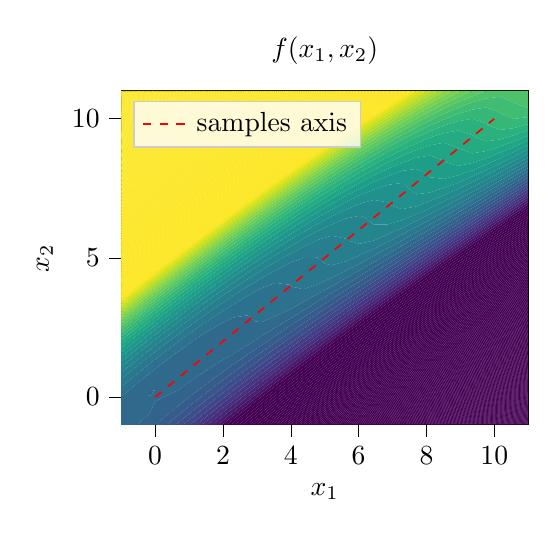
\begin{tikzpicture}

\definecolor{darkcyan30152138}{RGB}{30,152,138}
\definecolor{darkcyan30158136}{RGB}{30,158,136}
\definecolor{darkcyan32145140}{RGB}{32,145,140}
\definecolor{darkcyan34138141}{RGB}{34,138,141}
\definecolor{darkcyan36133141}{RGB}{36,133,141}
\definecolor{darkcyan39126142}{RGB}{39,126,142}
\definecolor{darkgray176}{RGB}{176,176,176}
\definecolor{darkslateblue5099141}{RGB}{50,99,141}
\definecolor{darkslateblue5393140}{RGB}{53,93,140}
\definecolor{darkslateblue5686139}{RGB}{56,86,139}
\definecolor{darkslateblue6078138}{RGB}{60,78,138}
\definecolor{darkslateblue6371136}{RGB}{63,71,136}
\definecolor{darkslateblue6662133}{RGB}{66,62,133}
\definecolor{darkslateblue6954129}{RGB}{69,54,129}
\definecolor{darkslateblue7047124}{RGB}{70,47,124}
\definecolor{darkslateblue7138118}{RGB}{71,38,118}
\definecolor{gold22822724}{RGB}{228,227,24}
\definecolor{gold24623031}{RGB}{246,230,31}
\definecolor{gold25323136}{RGB}{253,231,36}
\definecolor{greenyellow19422334}{RGB}{194,223,34}
\definecolor{greenyellow21022527}{RGB}{210,225,27}
\definecolor{indigo68184}{RGB}{68,1,84}
\definecolor{indigo70992}{RGB}{70,9,92}
\definecolor{indigo7120102}{RGB}{71,20,102}
\definecolor{indigo7229111}{RGB}{72,29,111}
\definecolor{lightgray204}{RGB}{204,204,204}
\definecolor{mediumseagreen10520491}{RGB}{105,204,91}
\definecolor{mediumseagreen32165133}{RGB}{32,165,133}
\definecolor{mediumseagreen37171129}{RGB}{37,171,129}
\definecolor{mediumseagreen43177125}{RGB}{43,177,125}
\definecolor{mediumseagreen53183120}{RGB}{53,183,120}
\definecolor{mediumseagreen64189114}{RGB}{64,189,114}
\definecolor{mediumseagreen77194107}{RGB}{77,194,107}
\definecolor{mediumseagreen9120098}{RGB}{91,200,98}
\definecolor{steelblue47106141}{RGB}{47,106,141}
\definecolor{teal41120142}{RGB}{41,120,142}
\definecolor{teal44113142}{RGB}{44,113,142}
\definecolor{yellowgreen12120981}{RGB}{121,209,81}
\definecolor{yellowgreen13921370}{RGB}{139,213,70}
\definecolor{yellowgreen15721758}{RGB}{157,217,58}
\definecolor{yellowgreen17522046}{RGB}{175,220,46}

\begin{axis}[
legend cell align={left},
legend style={
  fill opacity=0.8,
  draw opacity=1,
  text opacity=1,
  at={(0.03,0.97)},
  anchor=north west,
  draw=lightgray204
},
tick align=outside,
tick pos=left,
title={\(\displaystyle f(x_1, x_2)\)},
x grid style={darkgray176},
xlabel={\(\displaystyle x_1\)},
xmin=-1, xmax=11,
xtick style={color=black},
y grid style={darkgray176},
ylabel={\(\displaystyle x_2\)},
ymin=-1, ymax=11,
ytick style={color=black}
]
\addplot [draw=none, fill=indigo68184, forget plot]
table{%
x  y
11 -1
11 -0.997974577454952
10.997889066822 -1
11 -1
};
\addplot [draw=none, fill=indigo68184, forget plot]
table{%
x  y
11 -0.997974577454952
11 -0.965567816734181
10.9641141359732 -1
10.997889066822 -1
11 -0.997974577454952
};
\addplot [draw=none, fill=indigo68184, forget plot]
table{%
x  y
11 -0.965567816734181
11 -0.933161056013409
10.9303392051245 -1
10.9641141359732 -1
11 -0.965567816734181
};
\addplot [draw=none, fill=indigo68184, forget plot]
table{%
x  y
11 -0.933161056013409
11 -0.900754295292638
10.8965642742757 -1
10.9303392051245 -1
11 -0.933161056013409
};
\addplot [draw=none, fill=indigo68184, forget plot]
table{%
x  y
11 -0.900754295292638
11 -0.868347534571867
10.862789343427 -1
10.8965642742757 -1
11 -0.900754295292638
};
\addplot [draw=none, fill=indigo68184, forget plot]
table{%
x  y
11 -0.868347534571867
11 -0.835940773851096
10.8290144125782 -1
10.862789343427 -1
11 -0.868347534571867
};
\addplot [draw=none, fill=indigo68184, forget plot]
table{%
x  y
11 -0.835940773851096
11 -0.803534013130325
10.7952394817295 -1
10.8290144125782 -1
11 -0.835940773851096
};
\addplot [draw=none, fill=indigo68184, forget plot]
table{%
x  y
11 -0.803534013130325
11 -0.771127252409554
10.7614645508808 -1
10.7952394817295 -1
11 -0.803534013130325
};
\addplot [draw=none, fill=indigo68184, forget plot]
table{%
x  y
11 -0.771127252409554
11 -0.738720491688783
10.727689620032 -1
10.7614645508808 -1
11 -0.771127252409554
};
\addplot [draw=none, fill=indigo68184, forget plot]
table{%
x  y
11 -0.738720491688783
11 -0.706313730968011
10.6939146891833 -1
10.727689620032 -1
11 -0.738720491688783
};
\addplot [draw=none, fill=indigo68184, forget plot]
table{%
x  y
11 -0.706313730968011
11 -0.67390697024724
10.6601397583345 -1
10.6939146891833 -1
11 -0.706313730968011
};
\addplot [draw=none, fill=indigo68184, forget plot]
table{%
x  y
11 -0.67390697024724
11 -0.641500209526469
10.6263648274858 -1
10.6601397583345 -1
11 -0.67390697024724
};
\addplot [draw=none, fill=indigo68184, forget plot]
table{%
x  y
11 -0.641500209526469
11 -0.609093448805698
10.5925898966371 -1
10.6263648274858 -1
11 -0.641500209526469
};
\addplot [draw=none, fill=indigo68184, forget plot]
table{%
x  y
10.5862068965517 -1
10.5925898966371 -1
11 -0.609093448805698
11 -0.586206896551724
11 -0.576356459723599
10.9896999890564 -0.586206896551724
10.5862068965517 -0.972758770462749
10.5578232531042 -1
10.5862068965517 -1
};
\addplot [draw=none, fill=indigo68184, forget plot]
table{%
x  y
10.5862068965517 -0.972758770462749
10.9896999890564 -0.586206896551724
11 -0.576356459723599
11 -0.54282560266333
10.9546387830718 -0.586206896551724
10.5862068965517 -0.939169657968178
10.5228255158889 -1
10.5578232531042 -1
10.5862068965517 -0.972758770462749
};
\addplot [draw=none, fill=indigo68184, forget plot]
table{%
x  y
10.5862068965517 -0.939169657968178
10.9546387830718 -0.586206896551724
11 -0.54282560266333
11 -0.509294745603061
10.9195775770872 -0.586206896551724
10.5862068965517 -0.905580545473607
10.4878277786736 -1
10.5228255158889 -1
10.5862068965517 -0.939169657968178
};
\addplot [draw=none, fill=indigo68184, forget plot]
table{%
x  y
10.5862068965517 -0.905580545473607
10.9195775770872 -0.586206896551724
11 -0.509294745603061
11 -0.475763888542792
10.8845163711026 -0.586206896551724
10.5862068965517 -0.871991432979037
10.4528300414584 -1
10.4878277786736 -1
10.5862068965517 -0.905580545473607
};
\addplot [draw=none, fill=indigo68184, forget plot]
table{%
x  y
10.5862068965517 -0.871991432979037
10.8845163711026 -0.586206896551724
11 -0.475763888542792
11 -0.442233031482524
10.8494551651181 -0.586206896551724
10.5862068965517 -0.838402320484466
10.4178323042431 -1
10.4528300414584 -1
10.5862068965517 -0.871991432979037
};
\addplot [draw=none, fill=indigo68184, forget plot]
table{%
x  y
10.5862068965517 -0.838402320484466
10.8494551651181 -0.586206896551724
11 -0.442233031482524
11 -0.408702174422255
10.8143939591335 -0.586206896551724
10.5862068965517 -0.804813207989895
10.3828345670278 -1
10.4178323042431 -1
10.5862068965517 -0.838402320484466
};
\addplot [draw=none, fill=indigo68184, forget plot]
table{%
x  y
10.5862068965517 -0.804813207989895
10.8143939591335 -0.586206896551724
11 -0.408702174422255
11 -0.375171317361986
10.7793327531489 -0.586206896551724
10.5862068965517 -0.771224095495325
10.3478368298126 -1
10.3828345670278 -1
10.5862068965517 -0.804813207989895
};
\addplot [draw=none, fill=indigo68184, forget plot]
table{%
x  y
10.5862068965517 -0.771224095495325
10.7793327531489 -0.586206896551724
11 -0.375171317361986
11 -0.341640460301717
10.7442715471643 -0.586206896551724
10.5862068965517 -0.737634983000754
10.3128390925973 -1
10.3478368298126 -1
10.5862068965517 -0.771224095495325
};
\addplot [draw=none, fill=indigo68184, forget plot]
table{%
x  y
10.5862068965517 -0.737634983000754
10.7442715471643 -0.586206896551724
11 -0.341640460301717
11 -0.308109603241449
10.7092103411797 -0.586206896551724
10.5862068965517 -0.704045870506183
10.277841355382 -1
10.3128390925973 -1
10.5862068965517 -0.737634983000754
};
\addplot [draw=none, fill=indigo68184, forget plot]
table{%
x  y
10.5862068965517 -0.704045870506183
10.7092103411797 -0.586206896551724
11 -0.308109603241449
11 -0.27457874618118
10.6741491351951 -0.586206896551724
10.5862068965517 -0.670456758011613
10.2428436181668 -1
10.277841355382 -1
10.5862068965517 -0.704045870506183
};
\addplot [draw=none, fill=indigo68184, forget plot]
table{%
x  y
10.5862068965517 -0.670456758011613
10.6741491351951 -0.586206896551724
11 -0.27457874618118
11 -0.241047889120911
10.6390879292106 -0.586206896551724
10.5862068965517 -0.636867645517042
10.2078458809515 -1
10.2428436181668 -1
10.5862068965517 -0.670456758011613
};
\addplot [draw=none, fill=indigo68184, forget plot]
table{%
x  y
10.5862068965517 -0.636867645517042
10.6390879292106 -0.586206896551724
11 -0.241047889120911
11 -0.207517032060642
10.604026723226 -0.586206896551724
10.5862068965517 -0.603278533022471
10.1728481437362 -1
10.2078458809515 -1
10.5862068965517 -0.636867645517042
};
\addplot [draw=none, fill=indigo68184, forget plot]
table{%
x  y
10.1724137931034 -1
10.1728481437362 -1
10.5862068965517 -0.603278533022471
10.604026723226 -0.586206896551724
11 -0.207517032060642
11 -0.173986175000374
10.5862068965517 -0.569094821121013
10.5683166335916 -0.586206896551724
10.1724137931034 -0.965571646933858
10.1365520479704 -1
10.1724137931034 -1
};
\addplot [draw=none, fill=indigo68184, forget plot]
table{%
x  y
10.1724137931034 -0.965571646933858
10.5683166335916 -0.586206896551724
10.5862068965517 -0.569094821121013
11 -0.173986175000374
11 -0.172413793103448
11 -0.139306937338338
10.9652599073598 -0.172413793103448
10.5862068965517 -0.534296561034018
10.5319358902954 -0.586206896551724
10.1724137931034 -0.930710640172025
10.1002396360123 -1
10.1365520479704 -1
10.1724137931034 -0.965571646933858
};
\addplot [draw=none, fill=indigo68184, forget plot]
table{%
x  y
10.1724137931034 -0.930710640172025
10.5319358902954 -0.586206896551724
10.5862068965517 -0.534296561034018
10.9652599073598 -0.172413793103448
11 -0.139306937338338
11 -0.104571198455271
10.9288105750738 -0.172413793103448
10.5862068965517 -0.499498300947022
10.4955551469992 -0.586206896551724
10.1724137931034 -0.895849633410192
10.0639272240543 -1
10.1002396360123 -1
10.1724137931034 -0.930710640172025
};
\addplot [draw=none, fill=indigo68184, forget plot]
table{%
x  y
10.1724137931034 -0.895849633410192
10.4955551469992 -0.586206896551724
10.5862068965517 -0.499498300947022
10.9288105750738 -0.172413793103448
11 -0.104571198455271
11 -0.0698354595722051
10.8923612427879 -0.172413793103448
10.5862068965517 -0.464700040860026
10.459174403703 -0.586206896551724
10.1724137931034 -0.860988626648359
10.0276148120962 -1
10.0639272240543 -1
10.1724137931034 -0.895849633410192
};
\addplot [draw=none, fill=indigo68184, forget plot]
table{%
x  y
10.1724137931034 -0.860988626648359
10.459174403703 -0.586206896551724
10.5862068965517 -0.464700040860026
10.8923612427879 -0.172413793103448
11 -0.0698354595722051
11 -0.0350997206891388
10.8559119105019 -0.172413793103448
10.5862068965517 -0.429901780773031
10.4227936604067 -0.586206896551724
10.1724137931034 -0.826127619886525
9.99130240013817 -1
10.0276148120962 -1
10.1724137931034 -0.860988626648359
};
\addplot [draw=none, fill=indigo68184, forget plot]
table{%
x  y
10.1724137931034 -0.826127619886525
10.4227936604067 -0.586206896551724
10.5862068965517 -0.429901780773031
10.8559119105019 -0.172413793103448
11 -0.0350997206891388
11 -0.000363981806072472
10.819462578216 -0.172413793103448
10.5862068965517 -0.395103520686035
10.3864129171105 -0.586206896551724
10.1724137931034 -0.791266613124692
9.95498998818012 -1
9.99130240013817 -1
10.1724137931034 -0.826127619886525
};
\addplot [draw=none, fill=indigo68184, forget plot]
table{%
x  y
10.1724137931034 -0.791266613124692
10.3864129171105 -0.586206896551724
10.5862068965517 -0.395103520686035
10.819462578216 -0.172413793103448
11 -0.000363981806072472
11 0.0343717570769939
10.7830132459301 -0.172413793103448
10.5862068965517 -0.360305260599039
10.3500321738143 -0.586206896551724
10.1724137931034 -0.756405606362859
9.91867757622206 -1
9.95498998818012 -1
10.1724137931034 -0.791266613124692
};
\addplot [draw=none, fill=indigo68184, forget plot]
table{%
x  y
10.1724137931034 -0.756405606362859
10.3500321738143 -0.586206896551724
10.5862068965517 -0.360305260599039
10.7830132459301 -0.172413793103448
11 0.0343717570769939
11 0.0691074959600602
10.7465639136441 -0.172413793103448
10.5862068965517 -0.325507000512044
10.3136514305181 -0.586206896551724
10.1724137931034 -0.721544599601026
9.88236516426401 -1
9.91867757622206 -1
10.1724137931034 -0.756405606362859
};
\addplot [draw=none, fill=indigo68184, forget plot]
table{%
x  y
10.1724137931034 -0.721544599601026
10.3136514305181 -0.586206896551724
10.5862068965517 -0.325507000512044
10.7465639136441 -0.172413793103448
11 0.0691074959600602
11 0.103843234843127
10.7101145813582 -0.172413793103448
10.5862068965517 -0.290708740425048
10.2772706872219 -0.586206896551724
10.1724137931034 -0.686683592839193
9.84605275230596 -1
9.88236516426401 -1
10.1724137931034 -0.721544599601026
};
\addplot [draw=none, fill=indigo68184, forget plot]
table{%
x  y
10.1724137931034 -0.686683592839193
10.2772706872219 -0.586206896551724
10.5862068965517 -0.290708740425048
10.7101145813582 -0.172413793103448
11 0.103843234843127
11 0.138578973726193
10.6736652490722 -0.172413793103448
10.5862068965517 -0.255910480338052
10.2408899439256 -0.586206896551724
10.1724137931034 -0.65182258607736
9.80974034034791 -1
9.84605275230596 -1
10.1724137931034 -0.686683592839193
};
\addplot [draw=none, fill=indigo68184, forget plot]
table{%
x  y
10.1724137931034 -0.65182258607736
10.2408899439256 -0.586206896551724
10.5862068965517 -0.255910480338052
10.6736652490722 -0.172413793103448
11 0.138578973726193
11 0.173314712609259
10.6372159167863 -0.172413793103448
10.5862068965517 -0.221112220251057
10.2045092006294 -0.586206896551724
10.1724137931034 -0.616961579315527
9.77342792838985 -1
9.80974034034791 -1
10.1724137931034 -0.65182258607736
};
\addplot [draw=none, fill=indigo68184, forget plot]
table{%
x  y
9.75862068965517 -1
9.77342792838985 -1
10.1724137931034 -0.616961579315527
10.2045092006294 -0.586206896551724
10.5862068965517 -0.221112220251057
10.6372159167863 -0.172413793103448
11 0.173314712609259
11 0.208050451492326
10.6007665845004 -0.172413793103448
10.5862068965517 -0.186313960164061
10.1724137931034 -0.581946945467251
10.1679608704691 -0.586206896551724
9.75862068965517 -0.978541847302181
9.73627615367792 -1
9.75862068965517 -1
};
\addplot [draw=none, fill=indigo68184, forget plot]
table{%
x  y
9.75862068965517 -0.978541847302181
10.1679608704691 -0.586206896551724
10.1724137931034 -0.581946945467251
10.5862068965517 -0.186313960164061
10.6007665845004 -0.172413793103448
11 0.208050451492326
11 0.241379310344828
11 0.242838628829707
10.9984628575619 0.241379310344828
10.5862068965517 -0.150735313843001
10.5634595355384 -0.172413793103448
10.1724137931034 -0.545781707743167
10.1301573834233 -0.586206896551724
9.75862068965517 -0.942308831528325
9.6985464415296 -1
9.73627615367792 -1
9.75862068965517 -0.978541847302181
};
\addplot [draw=none, fill=indigo68184, forget plot]
table{%
x  y
9.75862068965517 -0.942308831528325
10.1301573834233 -0.586206896551724
10.1724137931034 -0.545781707743167
10.5634595355384 -0.172413793103448
10.5862068965517 -0.150735313843001
10.9984628575619 0.241379310344828
11 0.242838628829707
11 0.278869068338948
10.9605109517873 0.241379310344828
10.5862068965517 -0.114637601068767
10.5255819845179 -0.172413793103448
10.1724137931034 -0.509616470019083
10.0923538963775 -0.586206896551724
9.75862068965517 -0.906075815754469
9.66081672938128 -1
9.6985464415296 -1
9.75862068965517 -0.942308831528325
};
\addplot [draw=none, fill=indigo68184, forget plot]
table{%
x  y
9.75862068965517 -0.906075815754469
10.0923538963775 -0.586206896551724
10.1724137931034 -0.509616470019083
10.5255819845179 -0.172413793103448
10.5862068965517 -0.114637601068767
10.9605109517873 0.241379310344828
11 0.278869068338948
11 0.314899507848188
10.9225590460127 0.241379310344828
10.5862068965517 -0.0785398882945337
10.4877044334975 -0.172413793103448
10.1724137931034 -0.473451232294999
10.0545504093318 -0.586206896551724
9.75862068965517 -0.869842799980613
9.62308701723297 -1
9.66081672938128 -1
9.75862068965517 -0.906075815754469
};
\addplot [draw=none, fill=indigo68184, forget plot]
table{%
x  y
9.75862068965517 -0.869842799980613
10.0545504093318 -0.586206896551724
10.1724137931034 -0.473451232294999
10.4877044334975 -0.172413793103448
10.5862068965517 -0.0785398882945338
10.9225590460127 0.241379310344828
11 0.314899507848188
11 0.350929947357429
10.8846071402382 0.241379310344828
10.5862068965517 -0.0424421755203
10.4498268824771 -0.172413793103448
10.1724137931034 -0.437285994570915
10.016746922286 -0.586206896551724
9.75862068965517 -0.833609784206757
9.58535730508465 -1
9.62308701723297 -1
9.75862068965517 -0.869842799980613
};
\addplot [draw=none, fill=indigo68184, forget plot]
table{%
x  y
9.75862068965517 -0.833609784206757
10.016746922286 -0.586206896551724
10.1724137931034 -0.437285994570915
10.4498268824771 -0.172413793103448
10.5862068965517 -0.0424421755203
10.8846071402382 0.241379310344828
11 0.350929947357429
11 0.386960386866669
10.8466552344636 0.241379310344828
10.5862068965517 -0.00634446274606631
10.4119493314567 -0.172413793103448
10.1724137931034 -0.40112075684683
9.97894343524018 -0.586206896551724
9.75862068965517 -0.797376768432901
9.54762759293633 -1
9.58535730508465 -1
9.75862068965517 -0.833609784206757
};
\addplot [draw=none, fill=indigo68184, forget plot]
table{%
x  y
9.75862068965517 -0.797376768432901
9.97894343524018 -0.586206896551724
10.1724137931034 -0.40112075684683
10.4119493314567 -0.172413793103448
10.5862068965517 -0.00634446274606631
10.8466552344636 0.241379310344828
11 0.386960386866669
11 0.42299082637591
10.808703328689 0.241379310344828
10.5862068965517 0.0297532500281674
10.3740717804363 -0.172413793103448
10.1724137931034 -0.364955519122746
9.94113994819439 -0.586206896551724
9.75862068965517 -0.761143752659045
9.50989788078802 -1
9.54762759293633 -1
9.75862068965517 -0.797376768432901
};
\addplot [draw=none, fill=indigo68184, forget plot]
table{%
x  y
9.75862068965517 -0.761143752659045
9.94113994819439 -0.586206896551724
10.1724137931034 -0.364955519122746
10.3740717804363 -0.172413793103448
10.5862068965517 0.0297532500281674
10.808703328689 0.241379310344828
11 0.42299082637591
11 0.45902126588515
10.7707514229144 0.241379310344828
10.5862068965517 0.0658509628024011
10.3361942294159 -0.172413793103448
10.1724137931034 -0.328790281398662
9.9033364611486 -0.586206896551724
9.75862068965517 -0.724910736885189
9.4721681686397 -1
9.50989788078802 -1
9.75862068965517 -0.761143752659045
};
\addplot [draw=none, fill=indigo68184, forget plot]
table{%
x  y
9.75862068965517 -0.724910736885189
9.9033364611486 -0.586206896551724
10.1724137931034 -0.328790281398662
10.3361942294159 -0.172413793103448
10.5862068965517 0.0658509628024011
10.7707514229144 0.241379310344828
11 0.45902126588515
11 0.495051705394391
10.7327995171398 0.241379310344828
10.5862068965517 0.101948675576635
10.2983166783955 -0.172413793103448
10.1724137931034 -0.292625043674578
9.86553297410281 -0.586206896551724
9.75862068965517 -0.688677721111333
9.43443845649138 -1
9.4721681686397 -1
9.75862068965517 -0.724910736885189
};
\addplot [draw=none, fill=indigo68184, forget plot]
table{%
x  y
9.75862068965517 -0.688677721111333
9.86553297410281 -0.586206896551724
10.1724137931034 -0.292625043674578
10.2983166783955 -0.172413793103448
10.5862068965517 0.101948675576635
10.7327995171398 0.241379310344828
11 0.495051705394391
11 0.531082144903631
10.6948476113653 0.241379310344828
10.5862068965517 0.138046388350869
10.2604391273751 -0.172413793103448
10.1724137931034 -0.256459805950494
9.82772948705703 -0.586206896551724
9.75862068965517 -0.652444705337477
9.39670874434307 -1
9.43443845649138 -1
9.75862068965517 -0.688677721111333
};
\addplot [draw=none, fill=indigo68184, forget plot]
table{%
x  y
9.75862068965517 -0.652444705337477
9.82772948705703 -0.586206896551724
10.1724137931034 -0.256459805950494
10.2604391273751 -0.172413793103448
10.5862068965517 0.138046388350869
10.6948476113653 0.241379310344828
11 0.531082144903631
11 0.567112584412872
10.6568957055907 0.241379310344828
10.5862068965517 0.174144101125102
10.2225615763547 -0.172413793103448
10.1724137931034 -0.22029456822641
9.78992600001124 -0.586206896551724
9.75862068965517 -0.616211689563621
9.35897903219475 -1
9.39670874434307 -1
9.75862068965517 -0.652444705337477
};
\addplot [draw=none, fill=indigo68184, forget plot]
table{%
x  y
9.3448275862069 -1
9.35897903219475 -1
9.75862068965517 -0.616211689563621
9.78992600001124 -0.586206896551724
10.1724137931034 -0.22029456822641
10.2225615763547 -0.172413793103448
10.5862068965517 0.174144101125102
10.6568957055907 0.241379310344828
11 0.567112584412872
11 0.603143023922112
10.6189437998161 0.241379310344828
10.5862068965517 0.210241813899336
10.1846840253343 -0.172413793103448
10.1724137931034 -0.184129330502325
9.75862068965517 -0.579736133880164
9.75185804587955 -0.586206896551724
9.3448275862069 -0.976429400321786
9.32029166496461 -1
9.3448275862069 -1
};
\addplot [draw=none, fill=indigo68184, forget plot]
table{%
x  y
9.3448275862069 -0.976429400321786
9.75185804587955 -0.586206896551724
9.75862068965517 -0.579736133880164
10.1724137931035 -0.184129330502325
10.1846840253343 -0.172413793103448
10.5862068965517 0.210241813899336
10.6189437998161 0.241379310344828
11 0.603143023922112
11 0.639173463431353
10.5862068965517 0.24653193849172
10.5807787830927 0.241379310344828
10.1724137931034 -0.147013821024711
10.1457621656462 -0.172413793103448
9.75862068965517 -0.542092129336922
9.71251600755498 -0.586206896551724
9.3448275862069 -0.938711956003789
9.28102952247011 -1
9.32029166496461 -1
9.3448275862069 -0.976429400321786
};
\addplot [draw=none, fill=indigo68184, forget plot]
table{%
x  y
9.3448275862069 -0.938711956003789
9.71251600755498 -0.586206896551724
9.75862068965517 -0.542092129336922
10.1457621656462 -0.172413793103448
10.1724137931034 -0.147013821024711
10.5807787830927 0.241379310344828
10.5862068965517 0.24653193849172
11 0.639173463431353
11 0.655172413793103
11 0.675979440510427
10.9779930457907 0.655172413793103
10.5862068965517 0.284029918126438
10.5412759736257 0.241379310344828
10.1724137931034 -0.109442970822282
10.1063399056631 -0.172413793103448
9.75862068965517 -0.50444812479368
9.67317396923041 -0.586206896551724
9.3448275862069 -0.900994511685792
9.24176737997561 -1
9.28102952247011 -1
9.3448275862069 -0.938711956003789
};
\addplot [draw=none, fill=indigo68184, forget plot]
table{%
x  y
9.3448275862069 -0.900994511685792
9.67317396923041 -0.586206896551724
9.75862068965517 -0.50444812479368
10.1063399056631 -0.172413793103448
10.1724137931034 -0.109442970822282
10.5412759736257 0.241379310344828
10.5862068965517 0.284029918126438
10.9779930457907 0.655172413793103
11 0.675979440510427
11 0.713404831702555
10.9384093570004 0.655172413793103
10.5862068965517 0.321527897761156
10.5017731641586 0.241379310344828
10.1724137931034 -0.0718721206198523
10.0669176456801 -0.172413793103448
9.75862068965517 -0.466804120250438
9.63383193090584 -0.586206896551724
9.3448275862069 -0.863277067367795
9.20250523748111 -1
9.24176737997561 -1
9.3448275862069 -0.900994511685792
};
\addplot [draw=none, fill=indigo68184, forget plot]
table{%
x  y
9.3448275862069 -0.863277067367795
9.63383193090584 -0.586206896551724
9.75862068965517 -0.466804120250438
10.0669176456801 -0.172413793103448
10.1724137931034 -0.0718721206198523
10.5017731641586 0.241379310344828
10.5862068965517 0.321527897761156
10.9384093570004 0.655172413793103
11 0.713404831702555
11 0.750830222894682
10.8988256682101 0.655172413793103
10.5862068965517 0.359025877395874
10.4622703546915 0.241379310344828
10.1724137931034 -0.0343012704174231
10.0274953856971 -0.172413793103448
9.75862068965517 -0.429160115707196
9.59448989258127 -0.586206896551724
9.3448275862069 -0.825559623049798
9.16324309498661 -1
9.20250523748111 -1
9.3448275862069 -0.863277067367795
};
\addplot [draw=none, fill=indigo68184, forget plot]
table{%
x  y
9.3448275862069 -0.825559623049798
9.59448989258127 -0.586206896551724
9.75862068965517 -0.429160115707196
10.0274953856971 -0.172413793103448
10.1724137931034 -0.0343012704174231
10.4622703546915 0.241379310344828
10.5862068965517 0.359025877395874
10.8988256682101 0.655172413793103
11 0.750830222894682
11 0.78825561408681
10.8592419794198 0.655172413793103
10.5862068965517 0.396523857030592
10.4227675452245 0.241379310344828
10.1724137931034 0.00326957978500618
9.98807312571412 -0.172413793103448
9.75862068965517 -0.391516111163954
9.5551478542567 -0.586206896551724
9.3448275862069 -0.787842178731801
9.12398095249211 -1
9.16324309498661 -1
9.3448275862069 -0.825559623049798
};
\addplot [draw=none, fill=indigo68184, forget plot]
table{%
x  y
9.3448275862069 -0.787842178731801
9.5551478542567 -0.586206896551724
9.75862068965517 -0.391516111163954
9.98807312571412 -0.172413793103448
10.1724137931034 0.00326957978500617
10.4227675452245 0.241379310344828
10.5862068965517 0.396523857030592
10.8592419794198 0.655172413793103
11 0.78825561408681
11 0.825681005278938
10.8196582906295 0.655172413793103
10.5862068965517 0.43402183666531
10.3832647357574 0.241379310344828
10.1724137931034 0.0408404299874355
9.94865086573111 -0.172413793103448
9.75862068965517 -0.353872106620712
9.51580581593212 -0.586206896551724
9.3448275862069 -0.750124734413804
9.08471880999761 -1
9.12398095249211 -1
9.3448275862069 -0.787842178731801
};
\addplot [draw=none, fill=indigo68184, forget plot]
table{%
x  y
9.3448275862069 -0.750124734413804
9.51580581593212 -0.586206896551724
9.75862068965517 -0.353872106620712
9.94865086573111 -0.172413793103448
10.1724137931034 0.0408404299874355
10.3832647357574 0.241379310344828
10.5862068965517 0.43402183666531
10.8196582906295 0.655172413793103
11 0.825681005278938
11 0.863106396471066
10.7800746018392 0.655172413793103
10.5862068965517 0.471519816300028
10.3437619262904 0.241379310344828
10.1724137931034 0.0784112801898647
9.9092286057481 -0.172413793103448
9.75862068965517 -0.31622810207747
9.47646377760755 -0.586206896551724
9.3448275862069 -0.712407290095807
9.04545666750311 -1
9.08471880999761 -1
9.3448275862069 -0.750124734413804
};
\addplot [draw=none, fill=indigo68184, forget plot]
table{%
x  y
9.3448275862069 -0.712407290095807
9.47646377760755 -0.586206896551724
9.75862068965517 -0.31622810207747
9.9092286057481 -0.172413793103448
10.1724137931034 0.0784112801898647
10.3437619262904 0.241379310344828
10.5862068965517 0.471519816300028
10.7800746018392 0.655172413793103
11 0.863106396471066
11 0.900531787663194
10.7404909130489 0.655172413793103
10.5862068965517 0.509017795934746
10.3042591168233 0.241379310344828
10.1724137931034 0.115982130392294
9.8698063457651 -0.172413793103448
9.75862068965517 -0.278584097534228
9.43712173928298 -0.586206896551724
9.3448275862069 -0.67468984577781
9.00619452500861 -1
9.04545666750311 -1
9.3448275862069 -0.712407290095807
};
\addplot [draw=none, fill=indigo68184, forget plot]
table{%
x  y
9.3448275862069 -0.67468984577781
9.43712173928298 -0.586206896551724
9.75862068965517 -0.278584097534228
9.8698063457651 -0.172413793103448
10.1724137931034 0.115982130392294
10.3042591168233 0.241379310344828
10.5862068965517 0.509017795934746
10.7404909130489 0.655172413793103
11 0.900531787663194
11 0.937957178855322
10.7009072242585 0.655172413793103
10.5862068965517 0.546515775569464
10.2647563073563 0.241379310344828
10.1724137931034 0.153552980594723
9.83038408578209 -0.172413793103448
9.75862068965517 -0.240940092990986
9.39777970095841 -0.586206896551724
9.3448275862069 -0.636972401459813
8.96693238251411 -1
9.00619452500861 -1
9.3448275862069 -0.67468984577781
};
\addplot [draw=none, fill=indigo68184, forget plot]
table{%
x  y
8.93103448275862 -1
8.96693238251411 -1
9.3448275862069 -0.636972401459813
9.39777970095841 -0.586206896551724
9.75862068965517 -0.240940092990986
9.83038408578209 -0.172413793103448
10.1724137931034 0.153552980594723
10.2647563073563 0.241379310344828
10.5862068965517 0.546515775569464
10.7009072242585 0.655172413793103
11 0.937957178855322
11 0.97538257004745
10.6613235354682 0.655172413793103
10.5862068965517 0.584013755204182
10.2252534978892 0.241379310344828
10.1724137931034 0.191123830797153
9.79096182579908 -0.172413793103448
9.75862068965517 -0.203296088447744
9.35843766263383 -0.586206896551724
9.3448275862069 -0.599254957141816
8.93103448275862 -0.996630054188027
8.92752781309116 -1
8.93103448275862 -1
};
\addplot [draw=none, fill=indigo68184, forget plot]
table{%
x  y
8.93103448275862 -0.996630054188027
9.3448275862069 -0.599254957141816
9.35843766263383 -0.586206896551724
9.75862068965517 -0.203296088447744
9.79096182579908 -0.172413793103448
10.1724137931034 0.191123830797153
10.2252534978892 0.241379310344828
10.5862068965517 0.584013755204182
10.6613235354682 0.655172413793103
11 0.97538257004745
11 1.01280796123958
10.6217398466779 0.655172413793103
10.5862068965517 0.6215117348389
10.1857506884222 0.241379310344828
10.1724137931034 0.228694680999582
9.75862068965517 -0.165378099402097
9.75123850829235 -0.172413793103448
9.3448275862069 -0.560535879919962
9.31800393775182 -0.586206896551724
8.93103448275862 -0.957301354408403
8.88660348781333 -1
8.92752781309116 -1
8.93103448275862 -0.996630054188027
};
\addplot [draw=none, fill=indigo68184, forget plot]
table{%
x  y
8.93103448275862 -0.957301354408403
9.31800393775182 -0.586206896551724
9.3448275862069 -0.560535879919962
9.75123850829235 -0.172413793103448
9.75862068965517 -0.165378099402097
10.1724137931034 0.228694680999582
10.1857506884222 0.241379310344828
10.5862068965517 0.6215117348389
10.6217398466779 0.655172413793103
11 1.01280796123958
11 1.05023335243171
10.5862068965517 0.659164574430458
10.5819832033814 0.655172413793103
10.1724137931035 0.267271882171804
10.1451330521496 0.241379310344828
9.75862068965517 -0.12620875954054
9.71014019119758 -0.172413793103448
9.3448275862069 -0.52128702185872
9.27699280110696 -0.586206896551724
8.93103448275862 -0.91797265462878
8.84567916253551 -1
8.88660348781333 -1
8.93103448275862 -0.957301354408403
};
\addplot [draw=none, fill=indigo68184, forget plot]
table{%
x  y
8.93103448275862 -0.91797265462878
9.27699280110696 -0.586206896551724
9.3448275862069 -0.52128702185872
9.71014019119758 -0.172413793103448
9.75862068965517 -0.12620875954054
10.1451330521496 0.241379310344828
10.1724137931034 0.267271882171804
10.5819832033814 0.655172413793103
10.5862068965517 0.659164574430458
11 1.05023335243171
11 1.06896551724138
11 1.08841161731603
10.9793404688278 1.06896551724138
10.5862068965517 0.698175840615089
10.540709408683 0.655172413793104
10.1724137931034 0.306362025390001
10.1039471831633 0.241379310344828
9.75862068965517 -0.0870394196789835
9.66904187410281 -0.172413793103448
9.3448275862069 -0.482038163797479
9.23598166446209 -0.586206896551724
8.93103448275862 -0.878643954849156
8.80475483725768 -1
8.84567916253551 -1
8.93103448275862 -0.91797265462878
};
\addplot [draw=none, fill=indigo68184, forget plot]
table{%
x  y
8.93103448275862 -0.878643954849156
9.23598166446209 -0.586206896551724
9.3448275862069 -0.482038163797479
9.66904187410281 -0.172413793103448
9.75862068965517 -0.0870394196789835
10.1039471831633 0.241379310344828
10.1724137931034 0.306362025390001
10.540709408683 0.655172413793103
10.5862068965517 0.698175840615089
10.9793404688278 1.06896551724138
11 1.08841161731603
11 1.12734432414603
10.9379783721974 1.06896551724138
10.5862068965517 0.73718710679972
10.4994356139845 0.655172413793103
10.1724137931034 0.345452168608199
10.0627613141769 0.241379310344828
9.75862068965517 -0.0478700798174268
9.62794355700803 -0.172413793103448
9.3448275862069 -0.442789305736237
9.19497052781723 -0.586206896551724
8.93103448275862 -0.839315255069532
8.76383051197985 -1
8.80475483725768 -1
8.93103448275862 -0.878643954849156
};
\addplot [draw=none, fill=indigo68184, forget plot]
table{%
x  y
8.93103448275862 -0.839315255069532
9.19497052781723 -0.586206896551724
9.3448275862069 -0.442789305736237
9.62794355700803 -0.172413793103448
9.75862068965517 -0.0478700798174268
10.0627613141769 0.241379310344828
10.1724137931034 0.345452168608198
10.4994356139845 0.655172413793103
10.5862068965517 0.73718710679972
10.9379783721974 1.06896551724138
11 1.12734432414603
11 1.16627703097604
10.896616275567 1.06896551724138
10.5862068965517 0.77619837298435
10.4581618192861 0.655172413793103
10.1724137931034 0.384542311826396
10.0215754451906 0.241379310344828
9.75862068965517 -0.00870073995587016
9.58684523991326 -0.172413793103448
9.3448275862069 -0.403540447674995
9.15395939117236 -0.586206896551724
8.93103448275862 -0.799986555289909
8.72290618670203 -1
8.76383051197985 -1
8.93103448275862 -0.839315255069532
};
\addplot [draw=none, fill=indigo68184, forget plot]
table{%
x  y
8.93103448275862 -0.799986555289909
9.15395939117236 -0.586206896551724
9.3448275862069 -0.403540447674995
9.58684523991326 -0.172413793103448
9.75862068965517 -0.00870073995587017
10.0215754451906 0.241379310344828
10.1724137931034 0.384542311826396
10.4581618192861 0.655172413793103
10.5862068965517 0.77619837298435
10.896616275567 1.06896551724138
11 1.16627703097604
11 1.20520973780604
10.8552541789366 1.06896551724138
10.5862068965517 0.815209639168981
10.4168880245876 0.655172413793103
10.1724137931034 0.423632455044593
9.98038957620426 0.241379310344828
9.75862068965517 0.0304685999056865
9.54574692281848 -0.172413793103448
9.3448275862069 -0.364291589613753
9.1129482545275 -0.586206896551724
8.93103448275862 -0.760657855510285
8.6819818614242 -1
8.72290618670203 -1
8.93103448275862 -0.799986555289909
};
\addplot [draw=none, fill=indigo68184, forget plot]
table{%
x  y
8.93103448275862 -0.760657855510285
9.1129482545275 -0.586206896551724
9.3448275862069 -0.364291589613753
9.54574692281848 -0.172413793103448
9.75862068965517 0.0304685999056865
9.98038957620426 0.241379310344828
10.1724137931034 0.423632455044593
10.4168880245876 0.655172413793103
10.5862068965517 0.815209639168981
10.8552541789366 1.06896551724138
11 1.20520973780604
11 1.24414244463605
10.8138920823061 1.06896551724138
10.5862068965517 0.854220905353612
10.3756142298891 0.655172413793103
10.1724137931034 0.46272259826279
9.93920370721793 0.241379310344828
9.75862068965517 0.0696379397672432
9.50464860572371 -0.172413793103448
9.3448275862069 -0.325042731552511
9.07193711788264 -0.586206896551724
8.93103448275862 -0.721329155730661
8.64105753614637 -1
8.6819818614242 -1
8.93103448275862 -0.760657855510285
};
\addplot [draw=none, fill=indigo68184, forget plot]
table{%
x  y
8.93103448275862 -0.721329155730661
9.07193711788264 -0.586206896551724
9.3448275862069 -0.325042731552511
9.50464860572371 -0.172413793103448
9.75862068965517 0.0696379397672432
9.93920370721793 0.241379310344828
10.1724137931034 0.46272259826279
10.3756142298891 0.655172413793103
10.5862068965517 0.854220905353612
10.8138920823061 1.06896551724138
11 1.24414244463605
11 1.28307515146605
10.7725299856757 1.06896551724138
10.5862068965517 0.893232171538243
10.3343404351907 0.655172413793103
10.1724137931034 0.501812741480987
9.8980178382316 0.241379310344828
9.75862068965517 0.1088072796288
9.46355028862894 -0.172413793103448
9.3448275862069 -0.28579387349127
9.03092598123777 -0.586206896551724
8.93103448275862 -0.682000455951038
8.60013321086855 -1
8.64105753614637 -1
8.93103448275862 -0.721329155730661
};
\addplot [draw=none, fill=indigo68184, forget plot]
table{%
x  y
8.93103448275862 -0.682000455951038
9.03092598123777 -0.586206896551724
9.3448275862069 -0.28579387349127
9.46355028862894 -0.172413793103448
9.75862068965517 0.1088072796288
9.8980178382316 0.241379310344828
10.1724137931034 0.501812741480987
10.3343404351907 0.655172413793103
10.5862068965517 0.893232171538243
10.7725299856757 1.06896551724138
11 1.28307515146605
11 1.32200785829606
10.7311678890453 1.06896551724138
10.5862068965517 0.932243437722874
10.2930666404922 0.655172413793103
10.1724137931034 0.540902884699184
9.85683196924527 0.241379310344828
9.75862068965517 0.147976619490357
9.42245197153416 -0.172413793103448
9.3448275862069 -0.246545015430028
8.98991484459291 -0.586206896551724
8.93103448275862 -0.642671756171414
8.55920888559072 -1
8.60013321086855 -1
8.93103448275862 -0.682000455951038
};
\addplot [draw=none, fill=indigo68184, forget plot]
table{%
x  y
8.93103448275862 -0.642671756171414
8.9899148445929 -0.586206896551724
9.3448275862069 -0.246545015430028
9.42245197153416 -0.172413793103448
9.75862068965517 0.147976619490356
9.85683196924527 0.241379310344828
10.1724137931034 0.540902884699184
10.2930666404922 0.655172413793103
10.5862068965517 0.932243437722874
10.7311678890453 1.06896551724138
11 1.32200785829606
11 1.36094056512606
10.6898057924149 1.06896551724138
10.5862068965517 0.971254703907505
10.2517928457938 0.655172413793103
10.1724137931034 0.579993027917381
9.81564610025894 0.241379310344828
9.75862068965517 0.187145959351913
9.38135365443939 -0.172413793103448
9.3448275862069 -0.207296157368786
8.94890370794804 -0.586206896551724
8.93103448275862 -0.60334305639179
8.51828456031289 -1
8.55920888559072 -1
8.93103448275862 -0.642671756171414
};
\addplot [draw=none, fill=indigo68184, forget plot]
table{%
x  y
8.51724137931035 -1
8.51828456031289 -1
8.93103448275862 -0.60334305639179
8.94890370794804 -0.586206896551724
9.3448275862069 -0.207296157368786
9.38135365443939 -0.172413793103448
9.75862068965517 0.187145959351913
9.81564610025894 0.241379310344828
10.1724137931034 0.579993027917381
10.2517928457938 0.655172413793103
10.5862068965517 0.971254703907505
10.6898057924149 1.06896551724138
11 1.36094056512606
11 1.39987327195607
10.6484436957845 1.06896551724138
10.5862068965517 1.01026597009214
10.2105190510953 0.655172413793103
10.1724137931034 0.619083171135578
9.77446023127261 0.241379310344828
9.75862068965517 0.22631529921347
9.3448275862069 -0.167862506764604
9.3400523142684 -0.172413793103448
8.93103448275862 -0.563073163895168
8.90686726970648 -0.586206896551724
8.51724137931035 -0.959963483815025
8.47559720784294 -1
8.51724137931035 -1
};
\addplot [draw=none, fill=indigo68184, forget plot]
table{%
x  y
8.51724137931035 -0.959963483815025
8.90686726970648 -0.586206896551724
8.93103448275862 -0.563073163895168
9.3400523142684 -0.172413793103448
9.3448275862069 -0.167862506764604
9.75862068965517 0.22631529921347
9.77446023127261 0.241379310344828
10.1724137931034 0.619083171135578
10.2105190510953 0.655172413793103
10.5862068965517 1.01026597009214
10.6484436957845 1.06896551724138
11 1.39987327195607
11 1.43880597878607
10.6070815991541 1.06896551724138
10.5862068965517 1.04927723627677
10.1724137931035 0.658299778995489
10.1691039353024 0.655172413793103
9.75862068965517 0.266502636417143
9.73214639667001 0.241379310344828
9.3448275862069 -0.126952614329407
9.29712909502695 -0.172413793103448
8.93103448275862 -0.522076521378823
8.86403913605317 -0.586206896551724
8.51724137931035 -0.918879722525845
8.43286373943255 -1
8.47559720784294 -1
8.51724137931035 -0.959963483815025
};
\addplot [draw=none, fill=indigo68184, forget plot]
table{%
x  y
8.51724137931035 -0.918879722525845
8.86403913605317 -0.586206896551724
8.93103448275862 -0.522076521378823
9.29712909502695 -0.172413793103448
9.3448275862069 -0.126952614329407
9.73214639667001 0.241379310344828
9.75862068965517 0.266502636417143
10.1691039353024 0.655172413793103
10.1724137931034 0.658299778995489
10.5862068965517 1.04927723627677
10.6070815991541 1.06896551724138
11 1.43880597878607
11 1.47773868561608
10.5862068965517 1.08910110390748
10.5648036942602 1.06896551724138
10.1724137931034 0.69903726802095
10.1259892726003 0.655172413793103
9.75862068965517 0.307326145127331
9.6891276686893 0.241379310344828
9.3448275862069 -0.0860427218942103
9.25420587578551 -0.172413793103448
8.93103448275862 -0.481079878862477
8.82121100239985 -0.586206896551724
8.51724137931035 -0.877795961236665
8.39013027102216 -1
8.43286373943255 -1
8.51724137931035 -0.918879722525845
};
\addplot [draw=none, fill=indigo68184, forget plot]
table{%
x  y
8.51724137931035 -0.877795961236665
8.82121100239985 -0.586206896551724
8.93103448275862 -0.481079878862477
9.25420587578551 -0.172413793103448
9.3448275862069 -0.0860427218942102
9.6891276686893 0.241379310344828
9.75862068965517 0.307326145127331
10.1259892726003 0.655172413793103
10.1724137931034 0.69903726802095
10.5648036942602 1.06896551724138
10.5862068965517 1.08910110390748
11 1.47773868561608
11 1.48275862068966
11 1.51809455475095
10.9622762354123 1.48275862068966
10.5862068965517 1.12975293499212
10.5215926679983 1.06896551724138
10.1724137931034 0.739774757046411
10.0828746098982 0.655172413793103
9.75862068965517 0.34814965383752
9.64610894070858 0.241379310344828
9.3448275862069 -0.0451328294590136
9.21128265654407 -0.172413793103448
8.93103448275862 -0.440083236346131
8.77838286874654 -0.586206896551724
8.51724137931035 -0.836712199947485
8.34739680261177 -1
8.39013027102216 -1
8.51724137931035 -0.877795961236665
};
\addplot [draw=none, fill=indigo68184, forget plot]
table{%
x  y
8.51724137931035 -0.836712199947485
8.77838286874654 -0.586206896551724
8.93103448275862 -0.440083236346131
9.21128265654407 -0.172413793103448
9.3448275862069 -0.0451328294590136
9.64610894070858 0.241379310344828
9.75862068965517 0.348149653837519
10.0828746098982 0.655172413793103
10.1724137931034 0.739774757046411
10.5215926679983 1.06896551724138
10.5862068965517 1.12975293499212
10.9622762354123 1.48275862068966
11 1.51809455475095
11 1.55866108736155
10.9189684138703 1.48275862068966
10.5862068965517 1.17040476607675
10.4783816417364 1.06896551724138
10.1724137931034 0.780512246071872
10.0397599471961 0.655172413793103
9.75862068965517 0.388973162547708
9.60309021272786 0.241379310344828
9.3448275862069 -0.00422293702381701
9.16835943730262 -0.172413793103448
8.93103448275862 -0.399086593829786
8.73555473509322 -0.586206896551724
8.51724137931035 -0.795628438658305
8.30466333420138 -1
8.34739680261177 -1
8.51724137931035 -0.836712199947485
};
\addplot [draw=none, fill=indigo68184, forget plot]
table{%
x  y
8.51724137931035 -0.795628438658305
8.73555473509322 -0.586206896551724
8.93103448275862 -0.399086593829786
9.16835943730262 -0.172413793103448
9.3448275862069 -0.00422293702381697
9.60309021272787 0.241379310344828
9.75862068965517 0.388973162547708
10.0397599471961 0.655172413793103
10.1724137931034 0.780512246071872
10.4783816417364 1.06896551724138
10.5862068965517 1.17040476607675
10.9189684138703 1.48275862068966
11 1.55866108736155
11 1.59922761997214
10.8756605923284 1.48275862068966
10.5862068965517 1.21105659716138
10.4351706154745 1.06896551724138
10.1724137931034 0.821249735097333
9.99664528449397 0.655172413793103
9.75862068965517 0.429796671257896
9.56007148474715 0.241379310344828
9.3448275862069 0.0366869554113797
9.12543621806118 -0.172413793103448
8.93103448275862 -0.35808995131344
8.69272660143991 -0.586206896551724
8.51724137931035 -0.754544677369124
8.26192986579099 -1
8.30466333420138 -1
8.51724137931035 -0.795628438658305
};
\addplot [draw=none, fill=indigo68184, forget plot]
table{%
x  y
8.51724137931035 -0.754544677369124
8.69272660143991 -0.586206896551724
8.93103448275862 -0.35808995131344
9.12543621806118 -0.172413793103448
9.3448275862069 0.0366869554113796
9.56007148474715 0.241379310344828
9.75862068965517 0.429796671257896
9.99664528449397 0.655172413793103
10.1724137931034 0.821249735097333
10.4351706154745 1.06896551724138
10.5862068965517 1.21105659716138
10.8756605923284 1.48275862068966
11 1.59922761997214
11 1.63979415258274
10.8323527707865 1.48275862068966
10.5862068965517 1.25170842824601
10.3919595892127 1.06896551724138
10.1724137931034 0.861987224122794
9.95353062179187 0.655172413793103
9.75862068965517 0.470620179968084
9.51705275676643 0.241379310344828
9.3448275862069 0.0775968478465763
9.08251299881974 -0.172413793103448
8.93103448275862 -0.317093308797094
8.6498984677866 -0.586206896551724
8.51724137931035 -0.713460916079944
8.21919639738061 -1
8.26192986579099 -1
8.51724137931035 -0.754544677369124
};
\addplot [draw=none, fill=indigo68184, forget plot]
table{%
x  y
8.51724137931035 -0.713460916079944
8.6498984677866 -0.586206896551724
8.93103448275862 -0.317093308797094
9.08251299881974 -0.172413793103448
9.3448275862069 0.0775968478465763
9.51705275676643 0.241379310344828
9.75862068965517 0.470620179968084
9.95353062179187 0.655172413793103
10.1724137931034 0.861987224122794
10.3919595892127 1.06896551724138
10.5862068965517 1.25170842824601
10.8323527707865 1.48275862068966
11 1.63979415258274
11 1.68036068519334
10.7890449492446 1.48275862068966
10.5862068965517 1.29236025933065
10.3487485629508 1.06896551724138
10.1724137931034 0.902724713148255
9.91041595908977 0.655172413793103
9.75862068965517 0.511443688678273
9.47403402878572 0.241379310344828
9.3448275862069 0.118506740281773
9.0395897795783 -0.172413793103448
8.93103448275862 -0.276096666280749
8.60707033413328 -0.586206896551724
8.51724137931035 -0.672377154790764
8.17646292897022 -1
8.21919639738061 -1
8.51724137931035 -0.713460916079944
};
\addplot [draw=none, fill=indigo68184, forget plot]
table{%
x  y
8.51724137931035 -0.672377154790764
8.60707033413328 -0.586206896551724
8.93103448275862 -0.276096666280749
9.0395897795783 -0.172413793103448
9.3448275862069 0.118506740281773
9.47403402878572 0.241379310344828
9.75862068965517 0.511443688678273
9.91041595908977 0.655172413793103
10.1724137931034 0.902724713148255
10.3487485629508 1.06896551724138
10.5862068965517 1.29236025933065
10.7890449492446 1.48275862068966
11 1.68036068519334
11 1.72092721780393
10.7457371277027 1.48275862068966
10.5862068965517 1.33301209041528
10.3055375366889 1.06896551724138
10.1724137931034 0.943462202173716
9.86730129638767 0.655172413793103
9.75862068965517 0.552267197388461
9.431015300805 0.241379310344828
9.3448275862069 0.15941663271697
8.99666656033685 -0.172413793103448
8.93103448275862 -0.235100023764403
8.56424220047997 -0.586206896551724
8.51724137931035 -0.631293393501584
8.13372946055983 -1
8.17646292897022 -1
8.51724137931035 -0.672377154790764
};
\addplot [draw=none, fill=indigo68184, forget plot]
table{%
x  y
8.10344827586207 -1
8.13372946055983 -1
8.51724137931035 -0.631293393501584
8.56424220047997 -0.586206896551724
8.93103448275862 -0.235100023764403
8.99666656033685 -0.172413793103448
9.3448275862069 0.15941663271697
9.431015300805 0.241379310344828
9.75862068965517 0.552267197388461
9.86730129638767 0.655172413793103
10.1724137931034 0.943462202173716
10.3055375366889 1.06896551724138
10.5862068965517 1.33301209041528
10.7457371277027 1.48275862068966
11 1.72092721780393
11 1.76149375041453
10.7024293061608 1.48275862068966
10.5862068965517 1.37366392149991
10.262326510427 1.06896551724138
10.1724137931034 0.984199691199177
9.82418663368557 0.655172413793103
9.75862068965517 0.593090706098649
9.38799657282429 0.241379310344828
9.3448275862069 0.200326525152166
8.95374334109541 -0.172413793103448
8.93103448275862 -0.194103381248057
8.52141406682666 -0.586206896551724
8.51724137931035 -0.590209632212404
8.10344827586207 -0.987469240356652
8.09042005302995 -1
8.10344827586207 -1
};
\addplot [draw=none, fill=indigo68184, forget plot]
table{%
x  y
8.10344827586207 -0.987469240356652
8.51724137931035 -0.590209632212404
8.52141406682666 -0.586206896551724
8.93103448275862 -0.194103381248057
8.95374334109541 -0.172413793103448
9.3448275862069 0.200326525152166
9.38799657282429 0.241379310344828
9.75862068965517 0.593090706098649
9.82418663368557 0.655172413793103
10.1724137931034 0.984199691199177
10.262326510427 1.06896551724138
10.5862068965517 1.37366392149991
10.7024293061608 1.48275862068966
11 1.76149375041453
11 1.80206028302513
10.6591214846189 1.48275862068966
10.5862068965517 1.41431575258455
10.2191154841652 1.06896551724138
10.1724137931034 1.02493718022464
9.78107197098347 0.655172413793103
9.75862068965517 0.633914214808837
9.34497784484357 0.241379310344828
9.3448275862069 0.241236417587363
8.93103448275862 -0.15225165605055
8.9098808291885 -0.172413793103448
8.51724137931035 -0.547479958929357
8.47679390940033 -0.586206896551724
8.10344827586207 -0.944466460004474
8.04571008964587 -1
8.09042005302995 -1
8.10344827586207 -0.987469240356652
};
\addplot [draw=none, fill=indigo68184, forget plot]
table{%
x  y
8.10344827586207 -0.944466460004474
8.47679390940033 -0.586206896551724
8.51724137931035 -0.547479958929357
8.9098808291885 -0.172413793103448
8.93103448275862 -0.15225165605055
9.3448275862069 0.241236417587363
9.34497784484357 0.241379310344828
9.75862068965517 0.633914214808837
9.78107197098347 0.655172413793103
10.1724137931034 1.02493718022464
10.2191154841652 1.06896551724138
10.5862068965517 1.41431575258455
10.6591214846189 1.48275862068966
11 1.80206028302513
11 1.84262681563572
10.615813663077 1.48275862068966
10.5862068965517 1.45496758366918
10.1759044579033 1.06896551724138
10.1724137931034 1.0656746692501
9.75862068965517 0.675600423194613
9.73699266880856 0.655172413793103
9.3448275862069 0.283947834589427
9.29996252601431 0.241379310344828
8.93103448275862 -0.109439329052949
8.86496311379644 -0.172413793103448
8.51724137931035 -0.504572616595345
8.4319803107911 -0.586206896551724
8.10344827586207 -0.901463679652296
8.00100012626179 -1
8.04571008964587 -1
8.10344827586207 -0.944466460004474
};
\addplot [draw=none, fill=indigo68184, forget plot]
table{%
x  y
8.10344827586207 -0.901463679652296
8.4319803107911 -0.586206896551724
8.51724137931035 -0.504572616595345
8.86496311379644 -0.172413793103448
8.93103448275862 -0.109439329052949
9.29996252601431 0.241379310344828
9.3448275862069 0.283947834589427
9.73699266880856 0.655172413793103
9.75862068965517 0.675600423194613
10.1724137931034 1.0656746692501
10.1759044579033 1.06896551724138
10.5862068965517 1.45496758366918
10.615813663077 1.48275862068966
11 1.84262681563572
11 1.88319334824632
10.5862068965517 1.49618400055506
10.5718632280498 1.48275862068966
10.1724137931034 1.10805967318815
10.1308348068118 1.06896551724138
9.75862068965517 0.718223976382193
9.69186526168933 0.655172413793103
9.3448275862069 0.326665566130579
9.25494020891747 0.241379310344828
8.93103448275862 -0.0666270020553477
8.82004539840438 -0.172413793103448
8.51724137931035 -0.461665274261334
8.38716671218187 -0.586206896551724
8.10344827586207 -0.858460899300118
7.95629016287771 -1
8.00100012626179 -1
8.10344827586207 -0.901463679652296
};
\addplot [draw=none, fill=indigo68184, forget plot]
table{%
x  y
8.10344827586207 -0.858460899300118
8.38716671218187 -0.586206896551724
8.51724137931035 -0.461665274261334
8.82004539840438 -0.172413793103448
8.93103448275862 -0.0666270020553477
9.25494020891747 0.241379310344828
9.3448275862069 0.326665566130579
9.69186526168933 0.655172413793103
9.75862068965517 0.718223976382193
10.1308348068118 1.06896551724138
10.1724137931034 1.10805967318815
10.5718632280498 1.48275862068966
10.5862068965517 1.49618400055506
11 1.88319334824632
11 1.89655172413793
11 1.92495169644599
10.9695194028843 1.89655172413793
10.5862068965517 1.53862043735769
10.5265241621909 1.48275862068966
10.1724137931034 1.15058946237239
10.0856018179251 1.06896551724138
9.75862068965517 0.760847529569774
9.64673785457009 0.655172413793103
9.3448275862069 0.369383297671732
9.20991789182063 0.241379310344828
8.93103448275862 -0.0238146750577466
8.77512768301232 -0.172413793103448
8.51724137931035 -0.418757931927323
8.34235311357263 -0.586206896551724
8.10344827586207 -0.81545811894794
7.91158019949362 -1
7.95629016287771 -1
8.10344827586207 -0.858460899300118
};
\addplot [draw=none, fill=indigo68184, forget plot]
table{%
x  y
8.10344827586207 -0.81545811894794
8.34235311357263 -0.586206896551724
8.51724137931035 -0.418757931927323
8.77512768301232 -0.172413793103448
8.93103448275862 -0.0238146750577466
9.20991789182063 0.241379310344828
9.3448275862069 0.369383297671732
9.64673785457009 0.655172413793103
9.75862068965517 0.760847529569774
10.0856018179251 1.06896551724138
10.1724137931034 1.15058946237239
10.5265241621909 1.48275862068966
10.5862068965517 1.53862043735769
10.9695194028843 1.89655172413793
11 1.92495169644599
11 1.96729518978419
10.9240737613563 1.89655172413793
10.5862068965517 1.58105687416032
10.481185096332 1.48275862068966
10.1724137931034 1.19311925155662
10.0403688290384 1.06896551724138
9.75862068965517 0.803471082757354
9.60161044745085 0.655172413793103
9.3448275862069 0.412101029212884
9.1648955747238 0.241379310344828
8.93103448275862 0.0189976519398543
8.73020996762026 -0.172413793103448
8.51724137931035 -0.375850589593311
8.2975395149634 -0.586206896551724
8.10344827586207 -0.772455338595762
7.86687023610954 -1
7.91158019949362 -1
8.10344827586207 -0.81545811894794
};
\addplot [draw=none, fill=indigo68184, forget plot]
table{%
x  y
8.10344827586207 -0.772455338595762
8.2975395149634 -0.586206896551724
8.51724137931035 -0.375850589593311
8.73020996762026 -0.172413793103448
8.93103448275862 0.0189976519398543
9.1648955747238 0.241379310344828
9.3448275862069 0.412101029212884
9.60161044745085 0.655172413793103
9.75862068965517 0.803471082757354
10.0403688290384 1.06896551724138
10.1724137931034 1.19311925155662
10.481185096332 1.48275862068966
10.5862068965517 1.58105687416032
10.9240737613563 1.89655172413793
11 1.96729518978419
11 2.00963868312239
10.8786281198284 1.89655172413793
10.5862068965517 1.62349331096296
10.4358460304731 1.48275862068966
10.1724137931034 1.23564904074086
9.99513584015167 1.06896551724138
9.75862068965517 0.846094635944934
9.55648304033161 0.655172413793103
9.3448275862069 0.454818760754037
9.11987325762696 0.241379310344828
8.93103448275862 0.0618099789374554
8.68529225222819 -0.172413793103448
8.51724137931035 -0.3329432472593
8.25272591635417 -0.586206896551724
8.10344827586207 -0.729452558243584
7.82216027272546 -1
7.86687023610954 -1
8.10344827586207 -0.772455338595762
};
\addplot [draw=none, fill=indigo68184, forget plot]
table{%
x  y
8.10344827586207 -0.729452558243584
8.25272591635417 -0.586206896551724
8.51724137931035 -0.3329432472593
8.68529225222819 -0.172413793103448
8.93103448275862 0.0618099789374554
9.11987325762696 0.241379310344828
9.3448275862069 0.454818760754037
9.55648304033161 0.655172413793103
9.75862068965517 0.846094635944934
9.99513584015167 1.06896551724138
10.1724137931034 1.23564904074086
10.4358460304731 1.48275862068966
10.5862068965517 1.62349331096296
10.8786281198284 1.89655172413793
11 2.00963868312239
11 2.05198217646059
10.8331824783005 1.89655172413793
10.5862068965517 1.66592974776559
10.3905069646142 1.48275862068966
10.1724137931034 1.27817882992509
9.94990285126495 1.06896551724138
9.75862068965517 0.888718189132514
9.51135563321238 0.655172413793103
9.3448275862069 0.497536492295189
9.07485094053012 0.241379310344828
8.93103448275862 0.104622305935056
8.64037453683613 -0.172413793103448
8.51724137931035 -0.290035904925288
8.20791231774493 -0.586206896551724
8.10344827586207 -0.686449777891406
7.77745030934138 -1
7.82216027272546 -1
8.10344827586207 -0.729452558243584
};
\addplot [draw=none, fill=indigo68184, forget plot]
table{%
x  y
8.10344827586207 -0.686449777891406
8.20791231774493 -0.586206896551724
8.51724137931035 -0.290035904925288
8.64037453683613 -0.172413793103448
8.93103448275862 0.104622305935056
9.07485094053012 0.241379310344828
9.3448275862069 0.497536492295189
9.51135563321238 0.655172413793103
9.75862068965517 0.888718189132514
9.94990285126495 1.06896551724138
10.1724137931034 1.27817882992509
10.3905069646142 1.48275862068966
10.5862068965517 1.66592974776559
10.8331824783005 1.89655172413793
11 2.05198217646059
11 2.09432566979879
10.7877368367726 1.89655172413793
10.5862068965517 1.70836618456822
10.3451678987553 1.48275862068966
10.1724137931034 1.32070861910933
9.90466986237823 1.06896551724138
9.75862068965517 0.931341742320095
9.46622822609314 0.655172413793103
9.3448275862069 0.540254223836342
9.02982862343329 0.241379310344828
8.93103448275862 0.147434632932657
8.59545682144407 -0.172413793103448
8.51724137931035 -0.247128562591277
8.1630987191357 -0.586206896551724
8.10344827586207 -0.643446997539229
7.7327403459573 -1
7.77745030934138 -1
8.10344827586207 -0.686449777891406
};
\addplot [draw=none, fill=indigo68184, forget plot]
table{%
x  y
7.68965517241379 -1
7.7327403459573 -1
8.10344827586207 -0.643446997539229
8.1630987191357 -0.586206896551724
8.51724137931035 -0.247128562591277
8.59545682144407 -0.172413793103448
8.93103448275862 0.147434632932657
9.02982862343329 0.241379310344828
9.3448275862069 0.540254223836342
9.46622822609314 0.655172413793103
9.75862068965517 0.931341742320095
9.90466986237823 1.06896551724138
10.1724137931034 1.32070861910933
10.3451678987553 1.48275862068966
10.5862068965517 1.70836618456822
10.7877368367726 1.89655172413793
11 2.09432566979879
11 2.13666916313699
10.7422911952447 1.89655172413793
10.5862068965517 1.75080262137086
10.2998288328964 1.48275862068966
10.1724137931034 1.36323840829356
9.85943687349151 1.06896551724138
9.75862068965517 0.973965295507675
9.4211008189739 0.655172413793103
9.3448275862069 0.582971955377495
8.98480630633645 0.241379310344828
8.93103448275862 0.190246959930258
8.55053910605201 -0.172413793103448
8.51724137931035 -0.204221220257266
8.11828512052647 -0.586206896551724
8.10344827586207 -0.600444217187051
7.68965517241379 -0.998360677720638
7.68795158896608 -1
7.68965517241379 -1
};
\addplot [draw=none, fill=indigo68184, forget plot]
table{%
x  y
7.68965517241379 -0.998360677720638
8.10344827586207 -0.600444217187051
8.11828512052647 -0.586206896551724
8.51724137931035 -0.204221220257266
8.55053910605201 -0.172413793103448
8.93103448275862 0.190246959930258
8.98480630633645 0.241379310344828
9.3448275862069 0.582971955377495
9.4211008189739 0.655172413793103
9.75862068965517 0.973965295507675
9.85943687349151 1.06896551724138
10.1724137931034 1.36323840829356
10.2998288328964 1.48275862068966
10.5862068965517 1.75080262137086
10.7422911952447 1.89655172413793
11 2.13666916313699
11 2.17901265647519
10.6968455537168 1.89655172413793
10.5862068965517 1.79323905817349
10.2544897670375 1.48275862068966
10.1724137931034 1.4057681974778
9.81420388460478 1.06896551724138
9.75862068965517 1.01658884869526
9.37597341185466 0.655172413793103
9.3448275862069 0.625689686918647
8.93978398923961 0.241379310344828
8.93103448275862 0.233059286927859
8.51724137931035 -0.160798302222994
8.50505513740592 -0.172413793103448
8.10344827586207 -0.55610221077628
8.0720142764348 -0.586206896551724
7.68965517241379 -0.953250819661139
7.6410734317626 -1
7.68795158896608 -1
7.68965517241379 -0.998360677720638
};
\addplot [draw=none, fill=indigo68184, forget plot]
table{%
x  y
7.68965517241379 -0.953250819661139
8.0720142764348 -0.586206896551724
8.10344827586207 -0.55610221077628
8.50505513740592 -0.172413793103448
8.51724137931035 -0.160798302222994
8.93103448275862 0.233059286927859
8.93978398923961 0.241379310344828
9.3448275862069 0.625689686918647
9.37597341185466 0.655172413793103
9.75862068965517 1.01658884869526
9.81420388460478 1.06896551724138
10.1724137931034 1.4057681974778
10.2544897670375 1.48275862068966
10.5862068965517 1.79323905817349
10.6968455537168 1.89655172413793
11 2.17901265647519
11 2.22135614981339
10.6513999121889 1.89655172413793
10.5862068965517 1.83567549497613
10.2091507011786 1.48275862068966
10.1724137931034 1.44829798666203
9.76897089571806 1.06896551724138
9.75862068965517 1.05921240188284
9.3448275862069 0.669019323896133
9.33016133231079 0.655172413793103
8.93103448275862 0.277470021505949
8.89298974571334 0.241379310344828
8.51724137931035 -0.115897973211962
8.45794853842115 -0.172413793103448
8.10344827586207 -0.511097361115756
8.02502217596893 -0.586206896551724
7.68965517241379 -0.908140961601641
7.59419527455912 -1
7.6410734317626 -1
7.68965517241379 -0.953250819661139
};
\addplot [draw=none, fill=indigo68184, forget plot]
table{%
x  y
7.68965517241379 -0.908140961601641
8.02502217596893 -0.586206896551724
8.10344827586207 -0.511097361115756
8.45794853842115 -0.172413793103448
8.51724137931035 -0.115897973211962
8.89298974571334 0.241379310344828
8.93103448275862 0.277470021505949
9.33016133231079 0.655172413793103
9.3448275862069 0.669019323896133
9.75862068965517 1.05921240188284
9.76897089571806 1.06896551724138
10.1724137931034 1.44829798666203
10.2091507011786 1.48275862068966
10.5862068965517 1.83567549497613
10.6513999121889 1.89655172413793
11 2.22135614981339
11 2.26369964315159
10.6059542706609 1.89655172413793
10.5862068965517 1.87811193177876
10.1724137931035 1.49119912718617
10.1633883181436 1.48275862068966
9.75862068965517 1.1033521774573
9.72202551822882 1.06896551724138
9.3448275862069 0.713712061326301
9.28282405420428 0.655172413793103
8.93103448275862 0.322266314226552
8.84576808888452 0.241379310344828
8.51724137931035 -0.0709976442009303
8.41084193943637 -0.172413793103448
8.10344827586207 -0.466092511455233
7.97803007550306 -0.586206896551724
7.68965517241379 -0.863031103542143
7.54731711735565 -1
7.59419527455912 -1
7.68965517241379 -0.908140961601641
};
\addplot [draw=none, fill=indigo68184, forget plot]
table{%
x  y
7.68965517241379 -0.863031103542143
7.97803007550306 -0.586206896551724
8.10344827586207 -0.466092511455233
8.41084193943637 -0.172413793103448
8.51724137931035 -0.0709976442009303
8.84576808888452 0.241379310344828
8.93103448275862 0.322266314226552
9.28282405420428 0.655172413793103
9.3448275862069 0.713712061326301
9.72202551822882 1.06896551724138
9.75862068965517 1.1033521774573
10.1633883181436 1.48275862068966
10.1724137931034 1.49119912718617
10.5862068965517 1.87811193177876
10.6059542706609 1.89655172413793
11 2.26369964315159
11 2.3060431364898
10.5862068965517 1.92165018504714
10.5592408831555 1.89655172413793
10.1724137931034 1.53568618375376
10.1158180905446 1.48275862068966
9.75862068965517 1.14794183726895
9.67457205126216 1.06896551724138
9.3448275862069 0.758404798756469
9.23548677609777 0.655172413793103
8.93103448275862 0.367062606947154
8.7985464320557 0.241379310344828
8.51724137931035 -0.0260973151898986
8.3637353404516 -0.172413793103448
8.10344827586207 -0.421087661794709
7.93103797503719 -0.586206896551724
7.68965517241379 -0.817921245482644
7.50043896015217 -1
7.54731711735565 -1
7.68965517241379 -0.863031103542143
};
\addplot [draw=none, fill=indigo68184, forget plot]
table{%
x  y
7.68965517241379 -0.817921245482644
7.93103797503719 -0.586206896551724
8.10344827586207 -0.421087661794709
8.3637353404516 -0.172413793103448
8.51724137931035 -0.0260973151898986
8.7985464320557 0.241379310344828
8.93103448275862 0.367062606947154
9.23548677609777 0.655172413793103
9.3448275862069 0.758404798756469
9.67457205126216 1.06896551724138
9.75862068965517 1.14794183726895
10.1158180905446 1.48275862068966
10.1724137931034 1.53568618375376
10.5592408831555 1.89655172413793
10.5862068965517 1.92165018504714
11 2.3060431364898
11 2.31034482758621
11 2.35012933502708
10.9570510953054 2.31034482758621
10.5862068965517 1.96603510947798
10.5115533189212 1.89655172413793
10.1724137931034 1.58017324032135
10.0682478629457 1.48275862068966
9.75862068965517 1.1925314970806
9.6271185842955 1.06896551724138
9.3448275862069 0.803097536186636
9.18814949799126 0.655172413793103
8.93103448275862 0.411858899667757
8.75132477522688 0.241379310344828
8.51724137931035 0.018803013821133
8.31662874146683 -0.172413793103448
8.10344827586207 -0.376082812134185
7.88404587457132 -0.586206896551724
7.68965517241379 -0.772811387423146
7.4535608029487 -1
7.50043896015217 -1
7.68965517241379 -0.817921245482644
};
\addplot [draw=none, fill=indigo68184, forget plot]
table{%
x  y
7.68965517241379 -0.772811387423146
7.88404587457132 -0.586206896551724
8.10344827586207 -0.376082812134185
8.31662874146683 -0.172413793103448
8.51724137931035 0.018803013821133
8.75132477522688 0.241379310344828
8.93103448275862 0.411858899667757
9.18814949799126 0.655172413793103
9.3448275862069 0.803097536186636
9.6271185842955 1.06896551724138
9.75862068965517 1.1925314970806
10.0682478629457 1.48275862068966
10.1724137931034 1.58017324032135
10.5115533189212 1.89655172413793
10.5862068965517 1.96603510947798
10.9570510953054 2.31034482758621
11 2.35012933502708
11 2.39441259519124
10.9092456141597 2.31034482758621
10.5862068965517 2.01042003390882
10.4638657546869 1.89655172413793
10.1724137931034 1.62466029688895
10.0206776353468 1.48275862068966
9.75862068965517 1.23712115689224
9.57966511732884 1.06896551724138
9.3448275862069 0.847790273616804
9.14081221988475 0.655172413793103
8.93103448275862 0.456655192388359
8.70410311839806 0.241379310344828
8.51724137931035 0.0637033428321646
8.26952214248206 -0.172413793103448
8.10344827586207 -0.331077962473661
7.83705377410545 -0.586206896551724
7.68965517241379 -0.727701529363647
7.40668264574522 -1
7.4535608029487 -1
7.68965517241379 -0.772811387423146
};
\addplot [draw=none, fill=indigo68184, forget plot]
table{%
x  y
7.68965517241379 -0.727701529363647
7.83705377410545 -0.586206896551724
8.10344827586207 -0.331077962473661
8.26952214248206 -0.172413793103448
8.51724137931035 0.0637033428321646
8.70410311839806 0.241379310344828
8.93103448275862 0.456655192388359
9.14081221988475 0.655172413793103
9.3448275862069 0.847790273616804
9.57966511732884 1.06896551724138
9.75862068965517 1.23712115689224
10.0206776353468 1.48275862068966
10.1724137931034 1.62466029688895
10.4638657546869 1.89655172413793
10.5862068965517 2.01042003390882
10.9092456141597 2.31034482758621
11 2.39441259519124
11 2.43869585535539
10.8614401330141 2.31034482758621
10.5862068965517 2.05480495833966
10.4161781904526 1.89655172413793
10.1724137931034 1.66914735345654
9.97310740774784 1.48275862068966
9.75862068965517 1.28171081670389
9.53221165036218 1.06896551724138
9.3448275862069 0.892483011046972
9.09347494177824 0.655172413793103
8.93103448275862 0.501451485108962
8.65688146156924 0.241379310344828
8.51724137931035 0.108603671843196
8.22241554349729 -0.172413793103448
8.10344827586207 -0.286073112813137
7.79006167363958 -0.586206896551724
7.68965517241379 -0.682591671304149
7.35980448854175 -1
7.40668264574522 -1
7.68965517241379 -0.727701529363647
};
\addplot [draw=none, fill=indigo68184, forget plot]
table{%
x  y
7.68965517241379 -0.682591671304149
7.79006167363958 -0.586206896551724
8.10344827586207 -0.286073112813137
8.22241554349729 -0.172413793103448
8.51724137931035 0.108603671843196
8.65688146156924 0.241379310344828
8.93103448275862 0.501451485108962
9.09347494177824 0.655172413793103
9.3448275862069 0.892483011046972
9.53221165036218 1.06896551724138
9.75862068965517 1.28171081670389
9.97310740774784 1.48275862068966
10.1724137931034 1.66914735345654
10.4161781904526 1.89655172413793
10.5862068965517 2.05480495833966
10.8614401330141 2.31034482758621
11 2.43869585535539
11 2.48297911551955
10.8136346518684 2.31034482758621
10.5862068965517 2.0991898827705
10.3684906262182 1.89655172413793
10.1724137931034 1.71363441002413
9.9255371801489 1.48275862068966
9.75862068965517 1.32630047651554
9.48475818339552 1.06896551724138
9.3448275862069 0.937175748477139
9.04613766367173 0.655172413793103
8.93103448275862 0.546247777829564
8.60965980474041 0.241379310344828
8.51724137931035 0.153504000854228
8.17530894451252 -0.172413793103448
8.10344827586207 -0.241068263152613
7.74306957317371 -0.586206896551724
7.68965517241379 -0.637481813244651
7.31292633133827 -1
7.35980448854175 -1
7.68965517241379 -0.682591671304149
};
\addplot [draw=none, fill=indigo68184, forget plot]
table{%
x  y
7.27586206896552 -1
7.31292633133827 -1
7.68965517241379 -0.637481813244651
7.74306957317371 -0.586206896551724
8.10344827586207 -0.241068263152613
8.17530894451252 -0.172413793103448
8.51724137931035 0.153504000854228
8.60965980474041 0.241379310344828
8.93103448275862 0.546247777829564
9.04613766367173 0.655172413793103
9.3448275862069 0.937175748477139
9.48475818339552 1.06896551724138
9.75862068965517 1.32630047651554
9.9255371801489 1.48275862068966
10.1724137931034 1.71363441002413
10.3684906262182 1.89655172413793
10.5862068965517 2.0991898827705
10.8136346518684 2.31034482758621
11 2.48297911551955
11 2.5272623756837
10.7658291707227 2.31034482758621
10.5862068965517 2.14357480720134
10.3208030619839 1.89655172413793
10.1724137931034 1.75812146659173
9.87796695254997 1.48275862068966
9.75862068965517 1.37089013632719
9.43730471642886 1.06896551724138
9.3448275862069 0.981868485907307
8.99880038556523 0.655172413793103
8.93103448275862 0.591044070550167
8.56243814791159 0.241379310344828
8.51724137931035 0.19840432986526
8.12820234552774 -0.172413793103448
8.10344827586207 -0.196063413492089
7.69607747270784 -0.586206896551724
7.68965517241379 -0.592371955185152
7.27586206896552 -0.990069726943929
7.26554799686587 -1
7.27586206896552 -1
};
\addplot [draw=none, fill=indigo68184, forget plot]
table{%
x  y
7.27586206896552 -0.990069726943929
7.68965517241379 -0.592371955185152
7.69607747270784 -0.586206896551724
8.10344827586207 -0.196063413492089
8.12820234552774 -0.172413793103448
8.51724137931035 0.19840432986526
8.56243814791159 0.241379310344828
8.93103448275862 0.591044070550167
8.99880038556523 0.655172413793103
9.3448275862069 0.981868485907307
9.43730471642886 1.06896551724138
9.75862068965517 1.37089013632719
9.87796695254997 1.48275862068966
10.1724137931034 1.75812146659173
10.3208030619839 1.89655172413793
10.5862068965517 2.14357480720134
10.7658291707227 2.31034482758621
11 2.5272623756837
11 2.57154563584785
10.718023689577 2.31034482758621
10.5862068965517 2.18795973163218
10.2731154977496 1.89655172413793
10.1724137931034 1.80260852315932
9.83039672495104 1.48275862068966
9.75862068965517 1.41547979613883
9.3898512494622 1.06896551724138
9.3448275862069 1.02656122333747
8.95146310745872 0.655172413793103
8.93103448275862 0.635840363270769
8.51724137931035 0.243398444881477
8.51511249511131 0.241379310344828
8.10344827586207 -0.150015785596519
8.07995068634306 -0.172413793103448
7.68965517241379 -0.5453557638884
7.64701239969753 -0.586206896551724
7.27586206896552 -0.942635664380036
7.21628063649212 -1
7.26554799686587 -1
7.27586206896552 -0.990069726943929
};
\addplot [draw=none, fill=indigo68184, forget plot]
table{%
x  y
7.27586206896552 -0.942635664380036
7.64701239969753 -0.586206896551724
7.68965517241379 -0.5453557638884
8.07995068634306 -0.172413793103448
8.10344827586207 -0.150015785596519
8.51511249511131 0.241379310344828
8.51724137931035 0.243398444881477
8.93103448275862 0.635840363270769
8.95146310745872 0.655172413793103
9.3448275862069 1.02656122333747
9.3898512494622 1.06896551724138
9.75862068965517 1.41547979613883
9.83039672495104 1.48275862068966
10.1724137931034 1.80260852315932
10.2731154977496 1.89655172413793
10.5862068965517 2.18795973163218
10.718023689577 2.31034482758621
11 2.57154563584785
11 2.61582889601201
10.6702182084313 2.31034482758621
10.5862068965517 2.23234465606302
10.2254279335153 1.89655172413793
10.1724137931034 1.84709557972692
9.7828264973521 1.48275862068966
9.75862068965517 1.46006945595048
9.3448275862069 1.07136489319469
9.3422723462962 1.06896551724138
8.93103448275862 0.681874035648708
8.90274027328751 0.655172413793103
8.51724137931035 0.29048592204811
8.46546558734329 0.241379310344828
8.10344827586207 -0.102813344090924
8.03043094247967 -0.172413793103448
7.68965517241379 -0.498037795297741
7.59761916997643 -0.586206896551724
7.27586206896552 -0.895201601816143
7.16701327611836 -1
7.21628063649212 -1
7.27586206896552 -0.942635664380036
};
\addplot [draw=none, fill=indigo68184, forget plot]
table{%
x  y
7.27586206896552 -0.895201601816143
7.59761916997643 -0.586206896551724
7.68965517241379 -0.498037795297741
8.03043094247967 -0.172413793103448
8.10344827586207 -0.102813344090924
8.46546558734329 0.241379310344828
8.51724137931035 0.29048592204811
8.90274027328751 0.655172413793103
8.93103448275862 0.681874035648708
9.3422723462962 1.06896551724138
9.3448275862069 1.07136489319469
9.75862068965517 1.46006945595048
9.7828264973521 1.48275862068966
10.1724137931034 1.84709557972692
10.2254279335153 1.89655172413793
10.5862068965517 2.23234465606302
10.6702182084313 2.31034482758621
11 2.61582889601201
11 2.66011215617616
10.6224127272856 2.31034482758621
10.5862068965517 2.27672958049386
10.1777403692809 1.89655172413793
10.1724137931034 1.89158263629451
9.75862068965517 1.50571817657563
9.73404698340931 1.48275862068966
9.3448275862069 1.11822411355421
9.29236914130588 1.06896551724138
8.93103448275862 0.728847107120666
8.85296554683396 0.655172413793103
8.51724137931035 0.337573399214743
8.41581867957526 0.241379310344828
8.10344827586207 -0.0556109025853291
7.98091119861627 -0.172413793103448
7.68965517241379 -0.450719826707082
7.54822594025534 -0.586206896551724
7.27586206896552 -0.84776753925225
7.11774591574461 -1
7.16701327611836 -1
7.27586206896552 -0.895201601816143
};
\addplot [draw=none, fill=indigo68184, forget plot]
table{%
x  y
7.27586206896552 -0.84776753925225
7.54822594025534 -0.586206896551724
7.68965517241379 -0.450719826707082
7.98091119861627 -0.172413793103448
8.10344827586207 -0.0556109025853291
8.41581867957526 0.241379310344828
8.51724137931035 0.337573399214743
8.85296554683396 0.655172413793103
8.93103448275862 0.728847107120666
9.29236914130588 1.06896551724138
9.3448275862069 1.11822411355421
9.73404698340931 1.48275862068966
9.75862068965517 1.50571817657563
10.1724137931034 1.89158263629451
10.1777403692809 1.89655172413793
10.5862068965517 2.27672958049386
10.6224127272856 2.31034482758621
11 2.66011215617616
11 2.70439541634031
10.5862068965517 2.32163279699633
10.5740037525135 2.31034482758621
10.1724137931034 1.93797608733322
10.1278546132339 1.89655172413793
9.75862068965517 1.55246409638219
9.68401463490812 1.48275862068966
9.3448275862069 1.16508333391373
9.24246593631556 1.06896551724138
8.93103448275862 0.775820178592624
8.80319082038041 0.655172413793103
8.51724137931035 0.384660876381376
8.36617177180723 0.241379310344828
8.10344827586207 -0.00840846107973407
7.93139145475288 -0.172413793103448
7.68965517241379 -0.403401858116423
7.49883271053424 -0.586206896551724
7.27586206896552 -0.800333476688358
7.06847855537086 -1
7.11774591574461 -1
7.27586206896552 -0.84776753925225
};
\addplot [draw=none, fill=indigo68184, forget plot]
table{%
x  y
7.27586206896552 -0.800333476688358
7.49883271053424 -0.586206896551724
7.68965517241379 -0.403401858116423
7.93139145475288 -0.172413793103448
8.10344827586207 -0.00840846107973404
8.36617177180723 0.241379310344828
8.51724137931035 0.384660876381376
8.80319082038041 0.655172413793103
8.93103448275862 0.775820178592624
9.24246593631556 1.06896551724138
9.3448275862069 1.16508333391373
9.68401463490812 1.48275862068966
9.75862068965517 1.55246409638219
10.1278546132339 1.89655172413793
10.1724137931034 1.93797608733322
10.5740037525135 2.31034482758621
10.5862068965517 2.32163279699633
11 2.70439541634031
11 2.72413793103448
11 2.74985686792531
10.972056299605 2.72413793103448
10.5862068965517 2.36815375147798
10.5237111013104 2.31034482758621
10.1724137931034 1.98460925316236
10.0776924510718 1.89655172413793
9.75862068965517 1.59921001618876
9.63398228640694 1.48275862068966
9.3448275862069 1.21194255427326
9.19256273132524 1.06896551724138
8.93103448275862 0.822793250064582
8.75341609392686 0.655172413793103
8.51724137931035 0.431748353548009
8.3165248640392 0.241379310344828
8.10344827586207 0.038793980425861
7.88187171088949 -0.172413793103448
7.68965517241379 -0.356083889525765
7.44943948081314 -0.586206896551724
7.27586206896552 -0.752899414124465
7.01921119499711 -1
7.06847855537086 -1
7.27586206896552 -0.800333476688358
};
\addplot [draw=none, fill=indigo68184, forget plot]
table{%
x  y
7.27586206896552 -0.752899414124465
7.44943948081314 -0.586206896551724
7.68965517241379 -0.356083889525765
7.88187171088949 -0.172413793103448
8.10344827586207 0.038793980425861
8.3165248640392 0.241379310344828
8.51724137931035 0.431748353548009
8.75341609392686 0.655172413793103
8.93103448275862 0.822793250064582
9.19256273132524 1.06896551724138
9.3448275862069 1.21194255427326
9.63398228640694 1.48275862068966
9.75862068965517 1.59921001618876
10.0776924510718 1.89655172413793
10.1724137931034 1.98460925316236
10.5237111013104 2.31034482758621
10.5862068965517 2.36815375147798
10.972056299605 2.72413793103448
11 2.74985686792531
11 2.79626614978168
10.9216324786965 2.72413793103448
10.5862068965517 2.41467470595963
10.4734184501073 2.31034482758621
10.1724137931034 2.03124241899151
10.0275302889096 1.89655172413793
9.75862068965517 1.64595593599533
9.58394993790575 1.48275862068966
9.3448275862069 1.25880177463278
9.14265952633492 1.06896551724138
8.93103448275862 0.86976632153654
8.70364136747331 0.655172413793103
8.51724137931035 0.478835830714641
8.26687795627117 0.241379310344828
8.10344827586207 0.0859964219314561
7.83235196702609 -0.172413793103448
7.68965517241379 -0.308765920935106
7.40004625109204 -0.586206896551724
7.27586206896552 -0.705465351560572
6.96994383462336 -1
7.01921119499711 -1
7.27586206896552 -0.752899414124465
};
\addplot [draw=none, fill=indigo68184, forget plot]
table{%
x  y
7.27586206896552 -0.705465351560572
7.40004625109204 -0.586206896551724
7.68965517241379 -0.308765920935106
7.83235196702609 -0.172413793103448
8.10344827586207 0.0859964219314561
8.26687795627117 0.241379310344828
8.51724137931035 0.478835830714641
8.70364136747331 0.655172413793103
8.93103448275862 0.86976632153654
9.14265952633492 1.06896551724138
9.3448275862069 1.25880177463278
9.58394993790575 1.48275862068966
9.75862068965517 1.64595593599533
10.0275302889096 1.89655172413793
10.1724137931034 2.03124241899151
10.4734184501073 2.31034482758621
10.5862068965517 2.41467470595963
10.9216324786965 2.72413793103448
11 2.79626614978168
11 2.84267543163805
10.871208657788 2.72413793103448
10.5862068965517 2.46119566044129
10.4231257989041 2.31034482758621
10.1724137931034 2.07787558482066
9.97736812674744 1.89655172413793
9.75862068965517 1.6927018558019
9.53391758940456 1.48275862068966
9.3448275862069 1.3056609949923
9.0927563213446 1.06896551724138
8.93103448275862 0.916739393008498
8.65386664101976 0.655172413793103
8.51724137931035 0.525923307881274
8.21723104850314 0.241379310344828
8.10344827586207 0.133198863437051
7.7828322231627 -0.172413793103448
7.68965517241379 -0.261447952344447
7.35065302137094 -0.586206896551724
7.27586206896552 -0.658031288996679
6.9206764742496 -1
6.96994383462336 -1
7.27586206896552 -0.705465351560572
};
\addplot [draw=none, fill=indigo68184, forget plot]
table{%
x  y
7.27586206896552 -0.658031288996679
7.35065302137094 -0.586206896551724
7.68965517241379 -0.261447952344447
7.7828322231627 -0.172413793103448
8.10344827586207 0.133198863437051
8.21723104850314 0.241379310344828
8.51724137931035 0.525923307881274
8.65386664101976 0.655172413793103
8.93103448275862 0.916739393008497
9.0927563213446 1.06896551724138
9.3448275862069 1.3056609949923
9.53391758940456 1.48275862068966
9.75862068965517 1.6927018558019
9.97736812674744 1.89655172413793
10.1724137931034 2.07787558482066
10.4231257989041 2.31034482758621
10.5862068965517 2.46119566044129
10.871208657788 2.72413793103448
11 2.84267543163805
11 2.88908471349442
10.8207848368795 2.72413793103448
10.5862068965517 2.50771661492294
10.372833147701 2.31034482758621
10.1724137931034 2.1245087506498
9.92720596458527 1.89655172413793
9.75862068965517 1.73944777560847
9.48388524090338 1.48275862068966
9.3448275862069 1.35252021535183
9.04285311635428 1.06896551724138
8.93103448275862 0.963712464480456
8.60409191456621 0.655172413793103
8.51724137931035 0.573010785047907
8.16758414073511 0.241379310344828
8.10344827586207 0.180401304942646
7.7333124792993 -0.172413793103448
7.68965517241379 -0.214129983753788
7.30125979164984 -0.586206896551724
7.27586206896552 -0.610597226432786
6.87140911387585 -1
6.9206764742496 -1
7.27586206896552 -0.658031288996679
};
\addplot [draw=none, fill=indigo68184, forget plot]
table{%
x  y
6.86206896551724 -1
6.87140911387585 -1
7.27586206896552 -0.610597226432786
7.30125979164984 -0.586206896551724
7.68965517241379 -0.214129983753788
7.7333124792993 -0.172413793103448
8.10344827586207 0.180401304942646
8.16758414073511 0.241379310344828
8.51724137931035 0.573010785047907
8.60409191456621 0.655172413793103
8.93103448275862 0.963712464480456
9.04285311635428 1.06896551724138
9.3448275862069 1.35252021535183
9.48388524090338 1.48275862068966
9.75862068965517 1.73944777560847
9.92720596458527 1.89655172413793
10.1724137931034 2.1245087506498
10.372833147701 2.31034482758621
10.5862068965517 2.50771661492294
10.8207848368795 2.72413793103448
11 2.88908471349442
11 2.93549399535079
10.770361015971 2.72413793103448
10.5862068965517 2.55423756940459
10.3225404964979 2.31034482758621
10.1724137931034 2.17114191647895
9.87704380242311 1.89655172413793
9.75862068965517 1.78619369541504
9.43385289240219 1.48275862068966
9.3448275862069 1.39937943571135
8.99294991136396 1.06896551724138
8.93103448275862 1.01068553595241
8.55431718811266 0.655172413793103
8.51724137931035 0.62009826221454
8.11793723296708 0.241379310344828
8.10344827586207 0.227603746448241
7.68965517241379 -0.166523697190649
7.68347620340561 -0.172413793103448
7.27586206896552 -0.561974065644022
7.25057445475153 -0.586206896551724
6.86206896551724 -0.959470307958761
6.81999753088325 -1
6.86206896551724 -1
};
\addplot [draw=none, fill=indigo68184, forget plot]
table{%
x  y
6.86206896551724 -0.959470307958761
7.25057445475153 -0.586206896551724
7.27586206896552 -0.561974065644021
7.68347620340561 -0.172413793103448
7.68965517241379 -0.166523697190649
8.10344827586207 0.227603746448241
8.11793723296708 0.241379310344828
8.51724137931035 0.62009826221454
8.55431718811266 0.655172413793103
8.93103448275862 1.01068553595241
8.99294991136396 1.06896551724138
9.3448275862069 1.39937943571135
9.43385289240219 1.48275862068966
9.75862068965517 1.78619369541504
9.87704380242311 1.89655172413793
10.1724137931034 2.17114191647895
10.3225404964979 2.31034482758621
10.5862068965517 2.55423756940459
10.770361015971 2.72413793103448
11 2.93549399535079
11 2.98190327720717
10.7199371950625 2.72413793103448
10.5862068965517 2.60075852388624
10.2722478452948 2.31034482758621
10.1724137931034 2.21777508230809
9.82688164026095 1.89655172413793
9.75862068965517 1.83293961522161
9.38382054390101 1.48275862068966
9.3448275862069 1.44623865607087
8.94304670637363 1.06896551724138
8.93103448275862 1.05765860742437
8.51724137931034 0.667800887267056
8.50385308363687 0.655172413793103
8.10344827586207 0.276522220173336
8.06638689452928 0.241379310344828
7.68965517241379 -0.116770319536778
7.63128272759009 -0.172413793103448
7.27586206896552 -0.512092319782916
7.19852150433646 -0.586206896551724
6.86206896551724 -0.909459529773807
6.76808435120099 -1
6.81999753088325 -1
6.86206896551724 -0.959470307958761
};
\addplot [draw=none, fill=indigo68184, forget plot]
table{%
x  y
6.86206896551724 -0.909459529773807
7.19852150433646 -0.586206896551724
7.27586206896552 -0.512092319782916
7.63128272759009 -0.172413793103448
7.68965517241379 -0.116770319536778
8.06638689452928 0.241379310344828
8.10344827586207 0.276522220173336
8.50385308363687 0.655172413793103
8.51724137931035 0.667800887267056
8.93103448275862 1.05765860742437
8.94304670637363 1.06896551724138
9.3448275862069 1.44623865607087
9.38382054390101 1.48275862068966
9.75862068965517 1.83293961522161
9.82688164026095 1.89655172413793
10.1724137931034 2.21777508230809
10.2722478452948 2.31034482758621
10.5862068965517 2.60075852388624
10.7199371950625 2.72413793103448
11 2.98190327720717
11 3.02831255906354
10.669513374154 2.72413793103448
10.5862068965517 2.6472794783679
10.2219551940917 2.31034482758621
10.1724137931034 2.26440824813724
9.77671947809879 1.89655172413793
9.75862068965517 1.87968553502817
9.3448275862069 1.49362460565514
9.33318563597437 1.48275862068966
8.93103448275862 1.10645331728688
8.89108093945769 1.06896551724138
8.51724137931035 0.717299500452463
8.45137626843669 0.655172413793103
8.10344827586207 0.326147888622534
8.01405213251709 0.241379310344828
7.68965517241379 -0.0670169418829075
7.57908925177456 -0.172413793103448
7.27586206896552 -0.462210573921811
7.14646855392138 -0.586206896551724
6.86206896551724 -0.859448751588853
6.71617117151874 -1
6.76808435120099 -1
6.86206896551724 -0.909459529773807
};
\addplot [draw=none, fill=indigo68184, forget plot]
table{%
x  y
6.86206896551724 -0.859448751588853
7.14646855392138 -0.586206896551724
7.27586206896552 -0.462210573921811
7.57908925177456 -0.172413793103448
7.68965517241379 -0.0670169418829075
8.01405213251709 0.241379310344828
8.10344827586207 0.326147888622534
8.45137626843669 0.655172413793103
8.51724137931035 0.717299500452463
8.89108093945769 1.06896551724138
8.93103448275862 1.10645331728688
9.33318563597437 1.48275862068966
9.3448275862069 1.49362460565514
9.75862068965517 1.87968553502817
9.77671947809879 1.89655172413793
10.1724137931034 2.26440824813724
10.2219551940917 2.31034482758621
10.5862068965517 2.6472794783679
10.669513374154 2.72413793103448
11 3.02831255906354
11 3.07472184091991
10.6190895532455 2.72413793103448
10.5862068965517 2.69380043284955
10.1724137931034 2.31107672140698
10.1716213126 2.31034482758621
9.75862068965517 1.92794979812656
9.72480242205009 1.89655172413793
9.3448275862069 1.54287105014676
9.2804223883055 1.48275862068966
8.93103448275862 1.1558255241394
8.8384612978156 1.06896551724138
8.51724137931035 0.766798113637869
8.39889945323651 0.655172413793103
8.10344827586207 0.375773557071732
7.96171737050491 0.241379310344828
7.68965517241379 -0.0172635642290367
7.52689577595904 -0.172413793103448
7.27586206896552 -0.412328828060706
7.0944156035063 -0.586206896551724
6.86206896551724 -0.8094379734039
6.66425799183648 -1
6.71617117151874 -1
6.86206896551724 -0.859448751588853
};
\addplot [draw=none, fill=indigo68184, forget plot]
table{%
x  y
6.86206896551724 -0.8094379734039
7.0944156035063 -0.586206896551724
7.27586206896552 -0.412328828060706
7.52689577595904 -0.172413793103448
7.68965517241379 -0.0172635642290367
7.96171737050491 0.241379310344828
8.10344827586207 0.375773557071732
8.39889945323651 0.655172413793103
8.51724137931035 0.766798113637869
8.8384612978156 1.06896551724138
8.93103448275862 1.1558255241394
9.2804223883055 1.48275862068966
9.3448275862069 1.54287105014676
9.72480242205009 1.89655172413793
9.75862068965517 1.92794979812656
10.1716213126 2.31034482758621
10.1724137931034 2.31107672140698
10.5862068965517 2.69380043284955
10.6190895532455 2.72413793103448
11 3.07472184091991
11 3.12113112277628
10.5862068965517 2.74113959451705
10.5677003850746 2.72413793103448
10.1724137931034 2.36007355350836
10.1185684884519 2.31034482758621
9.75862068965517 1.97707111932071
9.67189478236936 1.89655172413793
9.3448275862069 1.59211749463837
9.22765914063664 1.48275862068966
8.93103448275862 1.20519773099192
8.7858416561735 1.06896551724138
8.51724137931035 0.816296726823275
8.34642263803633 0.655172413793103
8.10344827586207 0.42539922552093
7.90938260849273 0.241379310344828
7.68965517241379 0.0324898134248342
7.47470230014352 -0.172413793103448
7.27586206896552 -0.362447082199601
7.04236265309122 -0.586206896551724
6.86206896551724 -0.759427195218946
6.61234481215423 -1
6.66425799183648 -1
6.86206896551724 -0.8094379734039
};
\addplot [draw=none, fill=indigo68184, forget plot]
table{%
x  y
6.86206896551724 -0.759427195218946
7.04236265309122 -0.586206896551724
7.27586206896552 -0.362447082199601
7.47470230014352 -0.172413793103448
7.68965517241379 0.0324898134248342
7.90938260849273 0.241379310344828
8.10344827586207 0.42539922552093
8.34642263803633 0.655172413793103
8.51724137931035 0.816296726823275
8.7858416561735 1.06896551724138
8.93103448275862 1.20519773099192
9.22765914063664 1.48275862068966
9.3448275862069 1.59211749463837
9.67189478236936 1.89655172413793
9.75862068965517 1.97707111932071
10.1185684884519 2.31034482758621
10.1724137931034 2.36007355350836
10.5677003850746 2.72413793103448
10.5862068965517 2.74113959451705
11 3.12113112277628
11 3.13793103448276
11 3.16903362775431
10.9659652238723 3.13793103448276
10.5862068965517 2.79001256692067
10.5145015774617 2.72413793103448
10.1724137931034 2.40907038560973
10.0655156643037 2.31034482758621
9.75862068965517 2.02619244051487
9.61898714268863 1.89655172413793
9.3448275862069 1.64136393912999
9.17489589296778 1.48275862068966
8.93103448275862 1.25456993784444
8.73322201453141 1.06896551724138
8.51724137931035 0.865795340008682
8.29394582283615 0.655172413793103
8.10344827586207 0.475024893970128
7.85704784648055 0.241379310344828
7.68965517241379 0.082243191078705
7.42250882432799 -0.172413793103448
7.27586206896552 -0.312565336338496
6.99030970267615 -0.586206896551724
6.86206896551724 -0.709416417033992
6.56043163247197 -1
6.61234481215423 -1
6.86206896551724 -0.759427195218946
};
\addplot [draw=none, fill=indigo68184, forget plot]
table{%
x  y
6.86206896551724 -0.709416417033992
6.99030970267615 -0.586206896551724
7.27586206896552 -0.312565336338496
7.42250882432799 -0.172413793103448
7.68965517241379 0.082243191078705
7.85704784648055 0.241379310344828
8.10344827586207 0.475024893970128
8.29394582283615 0.655172413793103
8.51724137931035 0.865795340008682
8.73322201453141 1.06896551724138
8.93103448275862 1.25456993784444
9.17489589296778 1.48275862068966
9.3448275862069 1.64136393912999
9.61898714268863 1.89655172413793
9.75862068965517 2.02619244051487
10.0655156643037 2.31034482758621
10.1724137931034 2.40907038560973
10.5145015774617 2.72413793103448
10.5862068965517 2.79001256692067
10.9659652238723 3.13793103448276
11 3.16903362775431
11 3.21778336509409
10.9126196271834 3.13793103448276
10.5862068965517 2.83888553932429
10.4613027698487 2.72413793103448
10.1724137931034 2.4580672177111
10.0124628401555 2.31034482758621
9.75862068965517 2.07531376170903
9.5660795030079 1.89655172413793
9.3448275862069 1.6906103836216
9.12213264529891 1.48275862068966
8.93103448275862 1.30394214469697
8.68060237288931 1.06896551724138
8.51724137931035 0.915293953194088
8.24146900763597 0.655172413793103
8.10344827586207 0.524650562419326
7.80471308446837 0.241379310344828
7.68965517241379 0.131996568732576
7.37031534851247 -0.172413793103448
7.27586206896552 -0.262683590477391
6.93825675226107 -0.586206896551724
6.86206896551724 -0.659405638849038
6.50851845278972 -1
6.56043163247197 -1
6.86206896551724 -0.709416417033992
};
\addplot [draw=none, fill=indigo68184, forget plot]
table{%
x  y
6.86206896551724 -0.659405638849038
6.93825675226107 -0.586206896551724
7.27586206896552 -0.262683590477391
7.37031534851247 -0.172413793103448
7.68965517241379 0.131996568732576
7.80471308446837 0.241379310344828
8.10344827586207 0.524650562419326
8.24146900763597 0.655172413793103
8.51724137931035 0.915293953194088
8.68060237288931 1.06896551724138
8.93103448275862 1.30394214469696
9.12213264529891 1.48275862068966
9.3448275862069 1.6906103836216
9.5660795030079 1.89655172413793
9.75862068965517 2.07531376170903
10.0124628401555 2.31034482758621
10.1724137931034 2.4580672177111
10.4613027698487 2.72413793103448
10.5862068965517 2.83888553932429
10.9126196271834 3.13793103448276
11 3.21778336509409
11 3.26653310243386
10.8592740304945 3.13793103448276
10.5862068965517 2.88775851172792
10.4081039622358 2.72413793103448
10.1724137931034 2.50706404981248
9.95941001600732 2.31034482758621
9.75862068965517 2.12443508290318
9.51317186332717 1.89655172413793
9.3448275862069 1.73985682811322
9.06936939763004 1.48275862068966
8.93103448275862 1.35331435154949
8.62798273124722 1.06896551724138
8.51724137931035 0.964792566379495
8.18899219243579 0.655172413793103
8.10344827586207 0.574276230868524
7.75237832245619 0.241379310344828
7.68965517241379 0.181749946386447
7.31812187269695 -0.172413793103448
7.27586206896552 -0.212801844616286
6.88620380184599 -0.586206896551724
6.86206896551724 -0.609394860664085
6.45660527310746 -1
6.50851845278972 -1
6.86206896551724 -0.659405638849038
};
\addplot [draw=none, fill=indigo68184, forget plot]
table{%
x  y
6.44827586206897 -1
6.45660527310746 -1
6.86206896551724 -0.609394860664085
6.88620380184599 -0.586206896551724
7.27586206896552 -0.212801844616286
7.31812187269695 -0.172413793103448
7.68965517241379 0.181749946386447
7.75237832245619 0.241379310344828
8.10344827586207 0.574276230868524
8.18899219243579 0.655172413793104
8.51724137931035 0.964792566379495
8.62798273124722 1.06896551724138
8.93103448275862 1.35331435154949
9.06936939763004 1.48275862068966
9.3448275862069 1.73985682811322
9.51317186332717 1.89655172413793
9.75862068965517 2.12443508290318
9.95941001600732 2.31034482758621
10.1724137931034 2.50706404981248
10.4081039622358 2.72413793103448
10.5862068965517 2.88775851172792
10.8592740304945 3.13793103448276
11 3.26653310243386
11 3.31528283977364
10.8059284338056 3.13793103448276
10.5862068965517 2.93663148413154
10.3549051546229 2.72413793103448
10.1724137931034 2.55606088191385
9.90635719185913 2.31034482758621
9.75862068965517 2.17355640409734
9.46026422364644 1.89655172413793
9.3448275862069 1.78910327260484
9.01660614996118 1.48275862068966
8.93103448275862 1.40268655840201
8.57536308960512 1.06896551724138
8.51724137931035 1.0142911795649
8.13651537723561 0.655172413793103
8.10344827586207 0.623901899317721
7.70004356044401 0.241379310344828
7.68965517241379 0.231503324040318
7.27586206896552 -0.162403552247907
7.26536143343311 -0.172413793103448
6.86206896551724 -0.557920687303541
6.83256196184573 -0.586206896551724
6.44827586206897 -0.955601581475048
6.40221867075448 -1
6.44827586206897 -1
};
\addplot [draw=none, fill=indigo68184, forget plot]
table{%
x  y
6.44827586206897 -0.955601581475048
6.83256196184573 -0.586206896551724
6.86206896551724 -0.557920687303541
7.26536143343311 -0.172413793103448
7.27586206896552 -0.162403552247907
7.68965517241379 0.231503324040318
7.70004356044401 0.241379310344828
8.10344827586207 0.623901899317721
8.13651537723561 0.655172413793103
8.51724137931035 1.0142911795649
8.57536308960512 1.06896551724138
8.93103448275862 1.40268655840201
9.01660614996118 1.48275862068966
9.3448275862069 1.78910327260484
9.46026422364644 1.89655172413793
9.75862068965517 2.17355640409734
9.90635719185913 2.31034482758621
10.1724137931034 2.55606088191385
10.3549051546229 2.72413793103448
10.5862068965517 2.93663148413154
10.8059284338056 3.13793103448276
11 3.31528283977364
11 3.36403257711342
10.7525828371167 3.13793103448276
10.5862068965517 2.98550445653516
10.3017063470099 2.72413793103448
10.1724137931034 2.60505771401522
9.85330436771095 2.31034482758621
9.75862068965517 2.22267772529149
9.40735658396571 1.89655172413793
9.3448275862069 1.83834971709645
8.96384290229232 1.48275862068966
8.93103448275862 1.45205876525453
8.52274344796302 1.06896551724138
8.51724137931035 1.06378979275031
8.10344827586207 0.674520856820745
8.08292439525274 0.655172413793103
7.68965517241379 0.283420521256442
7.64530786121368 0.241379310344828
7.27586206896552 -0.109807768978807
7.21018901964 -0.172413793103448
6.86206896551724 -0.505181428381058
6.77754654804445 -0.586206896551724
6.44827586206897 -0.902718061985647
6.34735936595429 -1
6.40221867075448 -1
6.44827586206897 -0.955601581475048
};
\addplot [draw=none, fill=indigo68184, forget plot]
table{%
x  y
6.44827586206897 -0.902718061985647
6.77754654804445 -0.586206896551724
6.86206896551724 -0.505181428381058
7.21018901964 -0.172413793103448
7.27586206896552 -0.109807768978807
7.64530786121368 0.241379310344828
7.68965517241379 0.283420521256442
8.08292439525274 0.655172413793103
8.10344827586207 0.674520856820745
8.51724137931035 1.06378979275031
8.52274344796302 1.06896551724138
8.93103448275862 1.45205876525453
8.96384290229232 1.48275862068966
9.3448275862069 1.83834971709645
9.40735658396571 1.89655172413793
9.75862068965517 2.22267772529149
9.85330436771095 2.31034482758621
10.1724137931034 2.60505771401522
10.3017063470099 2.72413793103448
10.5862068965517 2.98550445653516
10.7525828371167 3.13793103448276
11 3.36403257711342
11 3.4127823144532
10.6992372404278 3.13793103448276
10.5862068965517 3.03437742893879
10.248507539397 2.72413793103448
10.1724137931034 2.65405454611659
9.80025154356277 2.31034482758621
9.75862068965517 2.27179904648565
9.35444894428498 1.89655172413793
9.3448275862069 1.88759616158807
8.93103448275862 1.50243598765766
8.90992758371836 1.48275862068966
8.51724137931035 1.11568046649039
8.46741135309055 1.06896551724138
8.10344827586207 0.726832018038332
8.02743527781672 0.655172413793103
7.68965517241379 0.33587360739707
7.58997754878821 0.241379310344828
7.27586206896552 -0.0572119857097068
7.1550166058469 -0.172413793103448
6.86206896551724 -0.452442169458576
6.72253113424317 -0.586206896551724
6.44827586206896 -0.849834542496247
6.2925000611541 -1
6.34735936595429 -1
6.44827586206897 -0.902718061985647
};
\addplot [draw=none, fill=indigo68184, forget plot]
table{%
x  y
6.44827586206897 -0.849834542496247
6.72253113424317 -0.586206896551724
6.86206896551724 -0.452442169458576
7.1550166058469 -0.172413793103448
7.27586206896552 -0.0572119857097067
7.58997754878821 0.241379310344828
7.68965517241379 0.33587360739707
8.02743527781672 0.655172413793103
8.10344827586207 0.726832018038332
8.46741135309055 1.06896551724138
8.51724137931035 1.11568046649039
8.90992758371836 1.48275862068966
8.93103448275862 1.50243598765766
9.3448275862069 1.88759616158807
9.35444894428498 1.89655172413793
9.75862068965517 2.27179904648565
9.80025154356277 2.31034482758621
10.1724137931034 2.65405454611659
10.248507539397 2.72413793103448
10.5862068965517 3.03437742893879
10.6992372404278 3.13793103448276
11 3.4127823144532
11 3.46153205179297
10.6458916437389 3.13793103448276
10.5862068965517 3.08325040134241
10.1953087317841 2.72413793103448
10.1724137931034 2.70305137821797
9.75862068965517 2.32148653534041
9.74653545475024 2.31034482758621
9.3448275862069 1.93900539106425
9.29903498190591 1.89655172413793
8.93103448275862 1.55446559070767
8.85411810572943 1.48275862068966
8.51724137931035 1.1678504687391
8.41176251643907 1.06896551724138
8.10344827586207 0.779143179255919
7.9719461603807 0.655172413793103
7.68965517241379 0.388326693537699
7.53464723636274 0.241379310344828
7.27586206896552 -0.00461620244060666
7.09984419205379 -0.172413793103448
6.86206896551724 -0.399702910536094
6.66751572044189 -0.586206896551724
6.44827586206897 -0.796951023006846
6.23764075635391 -1
6.2925000611541 -1
6.44827586206897 -0.849834542496247
};
\addplot [draw=none, fill=indigo68184, forget plot]
table{%
x  y
6.44827586206897 -0.796951023006846
6.66751572044189 -0.586206896551724
6.86206896551724 -0.399702910536094
7.09984419205379 -0.172413793103448
7.27586206896552 -0.00461620244060666
7.53464723636274 0.241379310344828
7.68965517241379 0.388326693537699
7.9719461603807 0.655172413793103
8.10344827586207 0.779143179255919
8.41176251643907 1.06896551724138
8.51724137931035 1.1678504687391
8.85411810572943 1.48275862068966
8.93103448275862 1.55446559070767
9.29903498190591 1.89655172413793
9.3448275862069 1.93900539106425
9.74653545475024 2.31034482758621
9.75862068965517 2.32148653534041
10.1724137931034 2.70305137821797
10.1953087317841 2.72413793103448
10.5862068965517 3.08325040134241
10.6458916437389 3.13793103448276
11 3.46153205179297
11 3.51028178913275
10.5925460470501 3.13793103448276
10.5862068965517 3.13212337374603
10.1724137931034 2.7535384143301
10.1403450786133 2.72413793103448
9.75862068965517 2.37323759489874
9.69040189559225 2.31034482758621
9.3448275862069 1.99089534856817
9.24306393244873 1.89655172413793
8.93103448275862 1.60649519375769
8.79830862774049 1.48275862068966
8.51724137931035 1.2200204709878
8.35611367978759 1.06896551724138
8.10344827586207 0.831454340473507
7.91645704294468 0.655172413793103
7.68965517241379 0.440779779678328
7.47931692393727 0.241379310344828
7.27586206896552 0.0479795808284934
7.04467177826069 -0.172413793103448
6.86206896551724 -0.346963651613611
6.61250030664061 -0.586206896551724
6.44827586206897 -0.744067503517446
6.18278145155372 -1
6.23764075635391 -1
6.44827586206897 -0.796951023006846
};
\addplot [draw=none, fill=indigo68184, forget plot]
table{%
x  y
6.44827586206897 -0.744067503517446
6.61250030664061 -0.586206896551724
6.86206896551724 -0.346963651613611
7.04467177826069 -0.172413793103448
7.27586206896552 0.0479795808284934
7.47931692393727 0.241379310344828
7.68965517241379 0.440779779678328
7.91645704294468 0.655172413793103
8.10344827586207 0.831454340473507
8.35611367978759 1.06896551724138
8.51724137931035 1.2200204709878
8.7983086277405 1.48275862068966
8.93103448275862 1.60649519375769
9.24306393244873 1.89655172413793
9.3448275862069 1.99089534856817
9.69040189559225 2.31034482758621
9.75862068965517 2.37323759489874
10.1403450786133 2.72413793103448
10.1724137931034 2.7535384143301
10.5862068965517 3.13212337374603
10.5925460470501 3.13793103448276
11 3.51028178913275
11 3.55172413793103
11 3.55941961526429
10.9915118715965 3.55172413793103
10.5862068965517 3.18328959549513
10.5364548803719 3.13793103448276
10.1724137931034 2.80515131755591
10.0840480633258 2.72413793103448
9.75862068965517 2.42498865445707
9.63426833643425 2.31034482758621
9.3448275862069 2.04278530607208
9.18709288299156 1.89655172413793
8.93103448275862 1.6585247968077
8.74249914975156 1.48275862068966
8.51724137931035 1.27219047323651
8.30046484313612 1.06896551724138
8.10344827586207 0.883765501691094
7.86096792550866 0.655172413793103
7.68965517241379 0.493232865818956
7.4239866115118 0.241379310344828
7.27586206896552 0.100575364097593
6.98949936446759 -0.172413793103448
6.86206896551724 -0.294224392691129
6.55748489283933 -0.586206896551724
6.44827586206897 -0.691183984028045
6.12792214675353 -1
6.18278145155372 -1
6.44827586206897 -0.744067503517446
};
\addplot [draw=none, fill=indigo68184, forget plot]
table{%
x  y
6.44827586206897 -0.691183984028045
6.55748489283933 -0.586206896551724
6.86206896551724 -0.294224392691129
6.98949936446759 -0.172413793103448
7.27586206896552 0.100575364097593
7.4239866115118 0.241379310344828
7.68965517241379 0.493232865818956
7.86096792550866 0.655172413793103
8.10344827586207 0.883765501691094
8.30046484313612 1.06896551724138
8.51724137931035 1.27219047323651
8.74249914975156 1.48275862068966
8.93103448275862 1.6585247968077
9.18709288299156 1.89655172413793
9.3448275862069 2.04278530607208
9.63426833643425 2.31034482758621
9.75862068965517 2.42498865445707
10.0840480633258 2.72413793103448
10.1724137931034 2.80515131755591
10.5364548803719 3.13793103448276
10.5862068965517 3.18328959549513
10.9915118715965 3.55172413793103
11 3.55941961526429
11 3.61075840703238
10.9348850714989 3.55172413793103
10.5862068965517 3.23476507807778
10.4799934542342 3.13793103448276
10.1724137931034 2.85676422078171
10.0277510480382 2.72413793103448
9.75862068965517 2.4767397140154
9.57813477727625 2.31034482758621
9.3448275862069 2.094675263576
9.13112183353438 1.89655172413793
8.93103448275862 1.71055439985771
8.68668967176263 1.48275862068966
8.51724137931035 1.32436047548522
8.24481600648464 1.06896551724138
8.10344827586207 0.936076662908682
7.80547880807264 0.655172413793103
7.68965517241379 0.545685951959585
7.36865629908633 0.241379310344828
7.27586206896552 0.153171147366694
6.93432695067448 -0.172413793103448
6.86206896551724 -0.241485133768646
6.50246947903805 -0.586206896551724
6.44827586206897 -0.638300464538645
6.07306284195334 -1
6.12792214675353 -1
6.44827586206897 -0.691183984028045
};
\addplot [draw=none, fill=indigo68184, forget plot]
table{%
x  y
6.03448275862069 -1
6.07306284195334 -1
6.44827586206896 -0.638300464538645
6.50246947903805 -0.586206896551724
6.86206896551724 -0.241485133768646
6.93432695067448 -0.172413793103448
7.27586206896552 0.153171147366694
7.36865629908633 0.241379310344828
7.68965517241379 0.545685951959585
7.80547880807264 0.655172413793103
8.10344827586207 0.936076662908682
8.24481600648464 1.06896551724138
8.51724137931035 1.32436047548522
8.68668967176263 1.48275862068966
8.93103448275862 1.71055439985771
9.13112183353438 1.89655172413793
9.3448275862069 2.094675263576
9.57813477727625 2.31034482758621
9.75862068965517 2.4767397140154
10.0277510480382 2.72413793103448
10.1724137931034 2.85676422078171
10.4799934542342 3.13793103448276
10.5862068965517 3.23476507807778
10.9348850714989 3.55172413793103
11 3.61075840703238
11 3.66209719880047
10.8782582714013 3.55172413793103
10.5862068965517 3.28624056066043
10.4235320280964 3.13793103448276
10.1724137931034 2.90837712400752
9.97145403275067 2.72413793103448
9.75862068965517 2.52849077357373
9.52200121811826 2.31034482758621
9.3448275862069 2.14656522107991
9.0751507840772 1.89655172413793
8.93103448275862 1.76258400290772
8.63088019377369 1.48275862068966
8.51724137931035 1.37653047773392
8.18916716983317 1.06896551724138
8.10344827586207 0.988387824126269
7.74998969063662 0.655172413793103
7.68965517241379 0.598139038100213
7.31332598666086 0.241379310344828
7.27586206896552 0.205766930635794
6.87915453688138 -0.172413793103448
6.86206896551724 -0.188745874846164
6.44827586206896 -0.585371228058505
6.44740447226726 -0.586206896551724
6.03448275862069 -0.983350706750615
6.01722409038649 -1
6.03448275862069 -1
};
\addplot [draw=none, fill=indigo68184, forget plot]
table{%
x  y
6.03448275862069 -0.983350706750615
6.44740447226726 -0.586206896551724
6.44827586206897 -0.585371228058505
6.86206896551724 -0.188745874846164
6.87915453688138 -0.172413793103448
7.27586206896552 0.205766930635794
7.31332598666086 0.241379310344828
7.68965517241379 0.598139038100213
7.74998969063662 0.655172413793103
8.10344827586207 0.988387824126269
8.18916716983317 1.06896551724138
8.51724137931035 1.37653047773392
8.63088019377369 1.48275862068966
8.93103448275862 1.76258400290772
9.0751507840772 1.89655172413793
9.3448275862069 2.14656522107991
9.52200121811826 2.31034482758621
9.75862068965517 2.52849077357373
9.97145403275067 2.72413793103448
10.1724137931034 2.90837712400752
10.4235320280964 3.13793103448276
10.5862068965517 3.28624056066043
10.8782582714013 3.55172413793103
11 3.66209719880047
11 3.71343599056856
10.8216314713036 3.55172413793103
10.5862068965517 3.33771604324308
10.3670706019587 3.13793103448276
10.1724137931034 2.95999002723332
9.91515701746312 2.72413793103448
9.75862068965517 2.58024183313206
9.46586765896026 2.31034482758621
9.3448275862069 2.19845517858382
9.01917973462002 1.89655172413793
8.93103448275862 1.81461360595773
8.57507071578476 1.48275862068966
8.51724137931035 1.42870047998263
8.13351833318169 1.06896551724138
8.10344827586207 1.04069898534386
7.6945005732006 0.655172413793103
7.68965517241379 0.650592124240842
7.27586206896552 0.259339941633116
7.25691094498286 0.241379310344828
6.86206896551724 -0.133905696826989
6.82167674044441 -0.172413793103448
6.44827586206897 -0.529427172114449
6.38906904355215 -0.586206896551724
6.03448275862069 -0.927244298044448
5.95906415055195 -1
6.01722409038649 -1
6.03448275862069 -0.983350706750615
};
\addplot [draw=none, fill=indigo68184, forget plot]
table{%
x  y
6.03448275862069 -0.927244298044448
6.38906904355215 -0.586206896551724
6.44827586206897 -0.529427172114449
6.82167674044441 -0.172413793103448
6.86206896551724 -0.133905696826989
7.25691094498286 0.241379310344828
7.27586206896552 0.259339941633116
7.68965517241379 0.650592124240842
7.6945005732006 0.655172413793103
8.10344827586207 1.04069898534386
8.13351833318169 1.06896551724138
8.51724137931035 1.42870047998263
8.57507071578476 1.48275862068966
8.93103448275862 1.81461360595773
9.01917973462002 1.89655172413793
9.3448275862069 2.19845517858382
9.46586765896026 2.31034482758621
9.75862068965517 2.58024183313206
9.91515701746312 2.72413793103448
10.1724137931034 2.95999002723332
10.3670706019587 3.13793103448276
10.5862068965517 3.33771604324308
10.8216314713036 3.55172413793103
11 3.71343599056856
11 3.76477478233665
10.765004671206 3.55172413793103
10.5862068965517 3.38919152582573
10.3106091758209 3.13793103448276
10.1724137931034 3.01160293045913
9.85886000217557 2.72413793103448
9.75862068965517 2.63199289269039
9.40973409980226 2.31034482758621
9.3448275862069 2.25034513608774
8.96320868516285 1.89655172413793
8.93103448275862 1.86664320900774
8.51926123779582 1.48275862068966
8.51724137931035 1.48087048223134
8.10344827586207 1.09438576301837
8.07630703609763 1.06896551724138
7.68965517241379 0.705791916377456
7.63592734208892 0.655172413793104
7.27586206896552 0.314962094594037
7.19822134214957 0.241379310344828
6.86206896551724 -0.0781230567692831
6.76316476062095 -0.172413793103448
6.44827586206897 -0.473483116170393
6.33073361483704 -0.586206896551724
6.03448275862069 -0.871137889338281
5.9009042107174 -1
5.95906415055195 -1
6.03448275862069 -0.927244298044448
};
\addplot [draw=none, fill=indigo68184, forget plot]
table{%
x  y
6.03448275862069 -0.871137889338281
6.33073361483704 -0.586206896551724
6.44827586206897 -0.473483116170393
6.76316476062095 -0.172413793103448
6.86206896551724 -0.0781230567692831
7.19822134214957 0.241379310344828
7.27586206896552 0.314962094594037
7.63592734208891 0.655172413793103
7.68965517241379 0.705791916377456
8.07630703609763 1.06896551724138
8.10344827586207 1.09438576301837
8.51724137931035 1.48087048223134
8.51926123779582 1.48275862068966
8.93103448275862 1.86664320900774
8.96320868516285 1.89655172413793
9.3448275862069 2.25034513608774
9.40973409980226 2.31034482758621
9.75862068965517 2.63199289269039
9.85886000217557 2.72413793103448
10.1724137931034 3.01160293045913
10.3106091758209 3.13793103448276
10.5862068965517 3.38919152582573
10.765004671206 3.55172413793103
11 3.76477478233665
11 3.81611357410474
10.7083778711084 3.55172413793103
10.5862068965517 3.44066700840838
10.2541477496832 3.13793103448276
10.1724137931034 3.06321583368494
9.80256298688802 2.72413793103448
9.75862068965517 2.68374395224873
9.35360054064427 2.31034482758621
9.3448275862069 2.30223509359165
8.93103448275862 1.91993118160048
8.90577508940792 1.89655172413793
8.51724137931035 1.53590895305853
8.46015599552789 1.48275862068966
8.10344827586207 1.14968969627225
8.01725893225441 1.06896551724138
7.68965517241379 0.761254503037748
7.57705903455276 0.655172413793103
7.27586206896552 0.370584247554958
7.13953173931628 0.241379310344828
6.86206896551724 -0.0223404167115769
6.7046527807975 -0.172413793103448
6.44827586206897 -0.417539060226337
6.27239818612192 -0.586206896551724
6.03448275862069 -0.815031480632114
5.84274427088286 -1
5.9009042107174 -1
6.03448275862069 -0.871137889338281
};
\addplot [draw=none, fill=indigo68184, forget plot]
table{%
x  y
6.03448275862069 -0.815031480632114
6.27239818612192 -0.586206896551724
6.44827586206897 -0.417539060226337
6.7046527807975 -0.172413793103448
6.86206896551724 -0.0223404167115769
7.13953173931628 0.241379310344828
7.27586206896552 0.370584247554958
7.57705903455276 0.655172413793103
7.68965517241379 0.761254503037748
8.01725893225441 1.06896551724138
8.10344827586207 1.14968969627225
8.46015599552789 1.48275862068966
8.51724137931035 1.53590895305853
8.90577508940792 1.89655172413793
8.93103448275862 1.91993118160048
9.3448275862069 2.30223509359165
9.35360054064427 2.31034482758621
9.75862068965517 2.68374395224873
9.80256298688802 2.72413793103448
10.1724137931034 3.06321583368494
10.2541477496832 3.13793103448276
10.5862068965517 3.44066700840838
10.7083778711084 3.55172413793103
11 3.81611357410474
11 3.86745236587283
10.6517510710107 3.55172413793103
10.5862068965517 3.49214249099103
10.1976863235455 3.13793103448276
10.1724137931034 3.11482873691074
9.75862068965517 2.73613741090803
9.74550195914668 2.72413793103448
9.3448275862069 2.35660844831661
9.2945472421765 2.31034482758621
8.93103448275862 1.97492051556587
8.84636407788423 1.89655172413793
8.51724137931035 1.59105513798841
8.40092699374081 1.48275862068966
8.10344827586207 1.20499362952612
7.95821082841119 1.06896551724138
7.68965517241379 0.81671708969804
7.5181907270166 0.655172413793103
7.27586206896552 0.426206400515878
7.08084213648299 0.241379310344828
6.86206896551724 0.0334422233461293
6.64614080097404 -0.172413793103448
6.44827586206897 -0.361595004282281
6.21406275740681 -0.586206896551724
6.03448275862069 -0.758925071925948
5.78458433104831 -1
5.84274427088286 -1
6.03448275862069 -0.815031480632114
};
\addplot [draw=none, fill=indigo68184, forget plot]
table{%
x  y
6.03448275862069 -0.758925071925948
6.21406275740681 -0.586206896551724
6.44827586206897 -0.361595004282281
6.64614080097404 -0.172413793103448
6.86206896551724 0.0334422233461293
7.08084213648299 0.241379310344828
7.27586206896552 0.426206400515878
7.5181907270166 0.655172413793103
7.68965517241379 0.81671708969804
7.95821082841119 1.06896551724138
8.10344827586207 1.20499362952612
8.40092699374081 1.48275862068966
8.51724137931035 1.59105513798841
8.84636407788423 1.89655172413793
8.93103448275862 1.97492051556587
9.2945472421765 2.31034482758621
9.3448275862069 2.35660844831661
9.74550195914668 2.72413793103448
9.75862068965517 2.73613741090803
10.1724137931034 3.11482873691074
10.1976863235455 3.13793103448276
10.5862068965517 3.49214249099103
10.6517510710107 3.55172413793103
11 3.86745236587283
11 3.91879115764092
10.5951242709131 3.55172413793103
10.5862068965517 3.54361797357368
10.1724137931034 3.16804975890433
10.1392902024046 3.13793103448276
9.75862068965517 2.79081570456817
9.68572355151978 2.72413793103448
9.3448275862069 2.41144182104174
9.23495309884231 2.31034482758621
8.93103448275862 2.02990984953127
8.78695306636055 1.89655172413793
8.51724137931035 1.64620132291829
8.34169799195373 1.48275862068966
8.10344827586207 1.26029756277999
7.89916272456798 1.06896551724138
7.68965517241379 0.872179676358331
7.45932241948044 0.655172413793103
7.27586206896552 0.481828553476799
7.02215253364969 0.241379310344828
6.86206896551724 0.0892248634038355
6.58762882115058 -0.172413793103448
6.44827586206897 -0.305650948338225
6.1557273286917 -0.586206896551724
6.03448275862069 -0.702818663219781
5.72642439121377 -1
5.78458433104831 -1
6.03448275862069 -0.758925071925948
};
\addplot [draw=none, fill=indigo68184, forget plot]
table{%
x  y
6.03448275862069 -0.702818663219781
6.1557273286917 -0.586206896551724
6.44827586206897 -0.305650948338225
6.58762882115058 -0.172413793103448
6.86206896551724 0.0892248634038354
7.02215253364969 0.241379310344828
7.27586206896552 0.481828553476799
7.45932241948044 0.655172413793103
7.68965517241379 0.872179676358331
7.89916272456798 1.06896551724138
8.10344827586207 1.26029756277999
8.34169799195373 1.48275862068966
8.51724137931035 1.64620132291829
8.78695306636055 1.89655172413793
8.93103448275862 2.02990984953127
9.23495309884231 2.31034482758621
9.3448275862069 2.41144182104174
9.68572355151978 2.72413793103448
9.75862068965517 2.79081570456817
10.1392902024046 3.13793103448276
10.1724137931034 3.16804975890433
10.5862068965517 3.54361797357368
10.5951242709131 3.55172413793103
11 3.91879115764092
11 3.96551724137931
11 3.97038866638193
10.9945787184431 3.96551724137931
10.5862068965517 3.59753278973356
10.5355287743735 3.55172413793103
10.1724137931034 3.22257384821103
10.0793263874654 3.13793103448276
9.75862068965517 2.84549399822832
9.62594514389288 2.72413793103448
9.3448275862069 2.46627519376686
9.17535895550812 2.31034482758621
8.93103448275862 2.08489918349666
8.72754205483686 1.89655172413793
8.51724137931035 1.70134750784817
8.28246899016665 1.48275862068966
8.10344827586207 1.31560149603387
7.84011462072476 1.06896551724138
7.68965517241379 0.927642263018623
7.40045411194428 0.655172413793103
7.27586206896552 0.53745070643772
6.9634629308164 0.241379310344828
6.86206896551724 0.145007503461542
6.52911684132713 -0.172413793103448
6.44827586206897 -0.24970689239417
6.09739189997659 -0.586206896551724
6.03448275862069 -0.646712254513614
5.66826445137922 -1
5.72642439121377 -1
6.03448275862069 -0.702818663219781
};
\addplot [draw=none, fill=indigo68184, forget plot]
table{%
x  y
5.62068965517241 -1
5.66826445137922 -1
6.03448275862069 -0.646712254513614
6.09739189997659 -0.586206896551724
6.44827586206897 -0.24970689239417
6.52911684132713 -0.172413793103448
6.86206896551724 0.145007503461542
6.9634629308164 0.241379310344828
7.27586206896552 0.53745070643772
7.40045411194428 0.655172413793103
7.68965517241379 0.927642263018623
7.84011462072476 1.06896551724138
8.10344827586207 1.31560149603387
8.28246899016665 1.48275862068966
8.51724137931035 1.70134750784817
8.72754205483686 1.89655172413793
8.93103448275862 2.08489918349666
9.17535895550812 2.31034482758621
9.3448275862069 2.46627519376686
9.62594514389288 2.72413793103448
9.75862068965517 2.84549399822832
10.0793263874654 3.13793103448276
10.1724137931034 3.22257384821103
10.5355287743735 3.55172413793103
10.5862068965517 3.59753278973356
10.9945787184431 3.96551724137931
11 3.97038866638193
11 4.0246069416799
10.9342406170127 3.96551724137931
10.5862068965517 3.65190354201854
10.4753783984337 3.55172413793104
10.1724137931034 3.27709793751773
10.0193625725261 3.13793103448276
9.75862068965517 2.90017229188847
9.56616673626598 2.72413793103448
9.3448275862069 2.52110856649198
9.11576481217393 2.31034482758621
8.93103448275862 2.13988851746206
8.66813104331317 1.89655172413793
8.51724137931035 1.75649369277805
8.22323998837956 1.48275862068966
8.10344827586207 1.37090542928774
7.78106651688154 1.06896551724138
7.68965517241379 0.983104849678915
7.34158580440812 0.655172413793103
7.27586206896552 0.59307285939864
6.90477332798311 0.241379310344828
6.86206896551724 0.200790143519248
6.47060486150367 -0.172413793103448
6.44827586206897 -0.193762836450114
6.03905647126148 -0.586206896551724
6.03448275862069 -0.590605845807447
5.62068965517241 -0.989125898034758
5.6094268816512 -1
5.62068965517241 -1
};
\addplot [draw=none, fill=indigo68184, forget plot]
table{%
x  y
5.62068965517241 -0.989125898034758
6.03448275862069 -0.590605845807447
6.03905647126148 -0.586206896551724
6.44827586206897 -0.193762836450114
6.47060486150368 -0.172413793103448
6.86206896551724 0.200790143519248
6.90477332798311 0.241379310344828
7.27586206896552 0.59307285939864
7.34158580440812 0.655172413793103
7.68965517241379 0.983104849678915
7.78106651688154 1.06896551724138
8.10344827586207 1.37090542928774
8.22323998837956 1.48275862068966
8.51724137931035 1.75649369277805
8.66813104331317 1.89655172413793
8.93103448275862 2.13988851746206
9.11576481217393 2.31034482758621
9.3448275862069 2.52110856649198
9.56616673626598 2.72413793103448
9.75862068965517 2.90017229188847
10.0193625725261 3.13793103448276
10.1724137931034 3.27709793751773
10.4753783984337 3.55172413793103
10.5862068965517 3.65190354201854
10.9342406170127 3.96551724137931
11 4.0246069416799
11 4.07882521697786
10.8739025155823 3.96551724137931
10.5862068965517 3.70627429430352
10.4152280224938 3.55172413793103
10.1724137931034 3.33162202682443
9.95939875758683 3.13793103448276
9.75862068965517 2.95485058554861
9.50638832863908 2.72413793103448
9.3448275862069 2.57594193921711
9.05617066883974 2.31034482758621
8.93103448275862 2.19487785142745
8.60872003178948 1.89655172413793
8.51724137931035 1.81163987770793
8.16401098659248 1.48275862068966
8.10344827586207 1.42620936254161
7.72201841303833 1.06896551724138
7.68965517241379 1.03856743633921
7.28271749687196 0.655172413793103
7.27586206896552 0.648695012359561
6.86206896551724 0.257503233583514
6.84505047503181 0.241379310344828
6.44827586206896 -0.135693670953108
6.40976162925249 -0.172413793103448
6.03448275862069 -0.531313354875836
5.97726832329086 -0.586206896551724
5.62068965517241 -0.929378280213486
5.54754371280617 -1
5.6094268816512 -1
5.62068965517241 -0.989125898034758
};
\addplot [draw=none, fill=indigo68184, forget plot]
table{%
x  y
5.62068965517241 -0.929378280213486
5.97726832329086 -0.586206896551724
6.03448275862069 -0.531313354875836
6.40976162925249 -0.172413793103448
6.44827586206897 -0.135693670953108
6.84505047503181 0.241379310344828
6.86206896551724 0.257503233583514
7.27586206896552 0.648695012359561
7.28271749687196 0.655172413793103
7.68965517241379 1.03856743633921
7.72201841303833 1.06896551724138
8.10344827586207 1.42620936254161
8.16401098659248 1.48275862068966
8.51724137931035 1.81163987770793
8.60872003178948 1.89655172413793
8.93103448275862 2.19487785142745
9.05617066883974 2.31034482758621
9.3448275862069 2.57594193921711
9.50638832863908 2.72413793103448
9.75862068965517 2.95485058554861
9.95939875758683 3.13793103448276
10.1724137931034 3.33162202682443
10.4152280224938 3.55172413793103
10.5862068965517 3.70627429430352
10.8739025155823 3.96551724137931
11 4.07882521697786
11 4.13304349227583
10.8135644141518 3.96551724137931
10.5862068965517 3.76064504658849
10.355077646554 3.55172413793103
10.1724137931034 3.38614611613112
9.89943494264757 3.13793103448276
9.75862068965517 3.00952887920876
9.44660992101218 2.72413793103448
9.3448275862069 2.63077531194223
8.99657652550555 2.31034482758621
8.93103448275862 2.24986718539285
8.5493090202658 1.89655172413793
8.51724137931035 1.8667860626378
8.1047819848054 1.48275862068966
8.10344827586207 1.48151329579549
7.68965517241379 1.09555563329165
7.66123423785532 1.06896551724138
7.27586206896552 0.707317608049195
7.22047629252113 0.655172413793104
6.86206896551724 0.316702008781269
6.78256730778161 0.241379310344828
6.44827586206896 -0.0763130720281017
6.34747975005786 -0.172413793103448
6.03448275862069 -0.471749811871985
5.91518643942679 -0.586206896551724
5.62068965517241 -0.869630662392213
5.48566054396115 -1
5.54754371280617 -1
5.62068965517241 -0.929378280213486
};
\addplot [draw=none, fill=indigo68184, forget plot]
table{%
x  y
5.62068965517241 -0.869630662392213
5.91518643942679 -0.586206896551724
6.03448275862069 -0.471749811871985
6.34747975005786 -0.172413793103448
6.44827586206896 -0.0763130720281017
6.78256730778161 0.241379310344828
6.86206896551724 0.316702008781269
7.22047629252113 0.655172413793103
7.27586206896552 0.707317608049195
7.66123423785532 1.06896551724138
7.68965517241379 1.09555563329165
8.10344827586207 1.48151329579549
8.1047819848054 1.48275862068966
8.51724137931035 1.8667860626378
8.5493090202658 1.89655172413793
8.93103448275862 2.24986718539285
8.99657652550555 2.31034482758621
9.3448275862069 2.63077531194223
9.44660992101218 2.72413793103448
9.75862068965517 3.00952887920876
9.89943494264757 3.13793103448276
10.1724137931034 3.38614611613112
10.355077646554 3.55172413793103
10.5862068965517 3.76064504658849
10.8135644141518 3.96551724137931
11 4.13304349227583
11 4.1872617675738
10.7532263127214 3.96551724137931
10.5862068965517 3.81501579887347
10.2949272706141 3.55172413793103
10.1724137931034 3.44067020543782
9.83947112770831 3.13793103448276
9.75862068965517 3.0642071728689
9.38683151338528 2.72413793103448
9.3448275862069 2.68560868466736
8.93698238217136 2.31034482758621
8.93103448275862 2.30485651935824
8.51724137931035 1.92346774684249
8.48810744695865 1.89655172413793
8.10344827586207 1.5400976502899
8.0417741224574 1.48275862068966
7.68965517241379 1.15439408117397
7.59834456585749 1.06896551724138
7.27586206896552 0.766335669611138
7.15779053191588 0.655172413793103
6.86206896551724 0.375900783979023
6.7200841405314 0.241379310344828
6.44827586206897 -0.0169324731030953
6.28519787086323 -0.172413793103448
6.03448275862069 -0.412186268868133
5.85310455556273 -0.586206896551724
5.62068965517241 -0.809883044570941
5.42377737511612 -1
5.48566054396115 -1
5.62068965517241 -0.869630662392213
};
\addplot [draw=none, fill=indigo68184, forget plot]
table{%
x  y
5.62068965517241 -0.809883044570941
5.85310455556273 -0.586206896551724
6.03448275862069 -0.412186268868133
6.28519787086323 -0.172413793103448
6.44827586206896 -0.0169324731030953
6.7200841405314 0.241379310344828
6.86206896551724 0.375900783979023
7.15779053191588 0.655172413793103
7.27586206896552 0.766335669611138
7.59834456585749 1.06896551724138
7.68965517241379 1.15439408117397
8.0417741224574 1.48275862068966
8.10344827586207 1.5400976502899
8.48810744695865 1.89655172413793
8.51724137931035 1.92346774684249
8.93103448275862 2.30485651935824
8.93698238217136 2.31034482758621
9.3448275862069 2.68560868466736
9.38683151338528 2.72413793103448
9.75862068965517 3.0642071728689
9.83947112770831 3.13793103448276
10.1724137931034 3.44067020543782
10.2949272706141 3.55172413793103
10.5862068965517 3.81501579887347
10.7532263127214 3.96551724137931
11 4.1872617675738
11 4.24148004287176
10.692888211291 3.96551724137931
10.5862068965517 3.86938655115845
10.2347768946743 3.55172413793103
10.1724137931034 3.49519429474452
9.77950731276905 3.13793103448276
9.75862068965517 3.11888546652905
9.3448275862069 2.74142251099457
9.32588148386669 2.72413793103448
8.93103448275862 2.36283158998536
8.87386371145114 2.31034482758621
8.51724137931035 1.98195022730631
8.42480594627652 1.89655172413793
8.10344827586207 1.59875757443655
7.97867920812506 1.48275862068966
7.68965517241379 1.21323252905629
7.53545489385966 1.06896551724138
7.27586206896552 0.825353731173081
7.09510477131064 0.655172413793103
6.86206896551724 0.435099559176778
6.6576009732812 0.241379310344828
6.44827586206897 0.0424481258219112
6.22291599166859 -0.172413793103448
6.03448275862069 -0.352622725864282
5.79102267169867 -0.586206896551724
5.62068965517241 -0.750135426749669
5.3618942062711 -1
5.42377737511612 -1
5.62068965517241 -0.809883044570941
};
\addplot [draw=none, fill=indigo68184, forget plot]
table{%
x  y
5.62068965517241 -0.750135426749669
5.79102267169867 -0.586206896551724
6.03448275862069 -0.352622725864282
6.22291599166859 -0.172413793103448
6.44827586206897 0.0424481258219112
6.6576009732812 0.241379310344828
6.86206896551724 0.435099559176778
7.09510477131064 0.655172413793103
7.27586206896552 0.825353731173081
7.53545489385966 1.06896551724138
7.68965517241379 1.21323252905629
7.97867920812506 1.48275862068966
8.10344827586207 1.59875757443655
8.42480594627652 1.89655172413793
8.51724137931035 1.98195022730631
8.87386371145114 2.31034482758621
8.93103448275862 2.36283158998536
9.32588148386669 2.72413793103448
9.3448275862069 2.74142251099457
9.75862068965517 3.11888546652905
9.77950731276905 3.13793103448276
10.1724137931034 3.49519429474452
10.2347768946743 3.55172413793103
10.5862068965517 3.86938655115845
10.692888211291 3.96551724137931
11 4.24148004287176
11 4.29569831816973
10.6325501098605 3.96551724137931
10.5862068965517 3.92375730344343
10.1746265187344 3.55172413793103
10.1724137931034 3.54971838405122
9.75862068965517 3.17570012146063
9.71695916990527 3.13793103448276
9.3448275862069 2.79955330528171
9.26216272528388 2.72413793103448
8.93103448275862 2.42113769704743
8.81035426715878 2.31034482758621
8.51724137931035 2.04043270777014
8.36150444559439 1.89655172413793
8.10344827586207 1.6574174985832
7.91558429379273 1.48275862068966
7.68965517241379 1.27207097693862
7.47256522186183 1.06896551724138
7.27586206896552 0.884371792735025
7.0324190107054 0.655172413793103
6.86206896551724 0.494298334374533
6.595117806031 0.241379310344828
6.44827586206897 0.101828724746918
6.16063411247396 -0.172413793103448
6.03448275862069 -0.293059182860431
5.72894078783461 -0.586206896551724
5.62068965517241 -0.690387808928397
5.30001103742607 -1
5.3618942062711 -1
5.62068965517241 -0.750135426749669
};
\addplot [draw=none, fill=indigo68184, forget plot]
table{%
x  y
5.62068965517241 -0.690387808928397
5.72894078783461 -0.586206896551724
6.03448275862069 -0.293059182860431
6.16063411247396 -0.172413793103448
6.44827586206896 0.101828724746918
6.595117806031 0.241379310344828
6.86206896551724 0.494298334374533
7.0324190107054 0.655172413793103
7.27586206896552 0.884371792735025
7.47256522186183 1.06896551724138
7.68965517241379 1.27207097693862
7.91558429379273 1.48275862068966
8.10344827586207 1.6574174985832
8.36150444559439 1.89655172413793
8.51724137931035 2.04043270777014
8.81035426715878 2.31034482758621
8.93103448275862 2.42113769704743
9.26216272528388 2.72413793103448
9.3448275862069 2.79955330528171
9.71695916990527 3.13793103448276
9.75862068965517 3.17570012146063
10.1724137931034 3.54971838405122
10.1746265187344 3.55172413793103
10.5862068965517 3.92375730344343
10.6325501098605 3.96551724137931
11 4.29569831816973
11 4.3499165934677
10.5862068965517 3.97887963145321
10.5712803099144 3.96551724137931
10.1724137931034 3.60738180100485
10.1106317866779 3.55172413793103
9.75862068965517 3.23365665406118
9.65302971275454 3.13793103448276
9.3448275862069 2.85768409956886
9.19844396670108 2.72413793103448
8.93103448275862 2.47944380410951
8.74684482286642 2.31034482758621
8.51724137931035 2.09891518823397
8.29820294491226 1.89655172413793
8.10344827586207 1.71607742272985
7.85248937946039 1.48275862068966
7.68965517241379 1.33090942482094
7.40967554986399 1.06896551724138
7.27586206896552 0.943389854296968
6.96973325010016 0.655172413793103
6.86206896551724 0.553497109572287
6.5326346387808 0.241379310344828
6.44827586206897 0.161209323671924
6.09835223327933 -0.172413793103448
6.03448275862069 -0.23349563985658
5.66685890397055 -0.586206896551724
5.62068965517241 -0.630640191107124
5.23812786858105 -1
5.30001103742607 -1
5.62068965517241 -0.690387808928397
};
\addplot [draw=none, fill=indigo68184, forget plot]
table{%
x  y
5.20689655172414 -1
5.23812786858105 -1
5.62068965517241 -0.630640191107124
5.66685890397055 -0.586206896551724
6.03448275862069 -0.23349563985658
6.09835223327933 -0.172413793103448
6.44827586206897 0.161209323671924
6.5326346387808 0.241379310344828
6.86206896551724 0.553497109572287
6.96973325010016 0.655172413793103
7.27586206896552 0.943389854296968
7.40967554986399 1.06896551724138
7.68965517241379 1.33090942482094
7.85248937946039 1.48275862068966
8.10344827586207 1.71607742272985
8.29820294491226 1.89655172413793
8.51724137931035 2.09891518823397
8.74684482286642 2.31034482758621
8.93103448275862 2.47944380410951
9.19844396670108 2.72413793103448
9.3448275862069 2.85768409956886
9.65302971275453 3.13793103448276
9.75862068965517 3.23365665406118
10.1106317866779 3.55172413793103
10.1724137931034 3.60738180100485
10.5712803099144 3.96551724137931
10.5862068965517 3.97887963145321
11 4.3499165934677
11 4.37931034482759
11 4.40560995808112
10.9704358090924 4.37931034482759
10.5862068965517 4.03649075636009
10.5069252475011 3.96551724137931
10.1724137931034 3.66516511358269
10.046490232904 3.55172413793103
9.75862068965517 3.29161318666173
9.5891002556038 3.13793103448276
9.3448275862069 2.915814893856
9.13472520811827 2.72413793103448
8.93103448275862 2.53774991117158
8.68333537857406 2.31034482758621
8.51724137931035 2.15739766869779
8.23490144423014 1.89655172413793
8.10344827586207 1.7747373468765
7.78939446512805 1.48275862068966
7.68965517241379 1.38974787270326
7.34678587786616 1.06896551724138
7.27586206896552 1.00240791585891
6.90704748949492 0.655172413793103
6.86206896551724 0.612695884770042
6.4701514715306 0.241379310344828
6.44827586206897 0.220589922596931
6.0360703540847 -0.172413793103448
6.03448275862069 -0.173932096852729
5.62068965517241 -0.569883669200261
5.60368493191208 -0.586206896551724
5.20689655172414 -0.968352026135101
5.17414824932931 -1
5.20689655172414 -1
};
\addplot [draw=none, fill=indigo68184, forget plot]
table{%
x  y
5.20689655172414 -0.968352026135101
5.60368493191208 -0.586206896551724
5.62068965517241 -0.569883669200261
6.03448275862069 -0.173932096852729
6.0360703540847 -0.172413793103448
6.44827586206897 0.220589922596931
6.4701514715306 0.241379310344828
6.86206896551724 0.612695884770042
6.90704748949492 0.655172413793103
7.27586206896552 1.00240791585891
7.34678587786616 1.06896551724138
7.68965517241379 1.38974787270326
7.78939446512805 1.48275862068966
8.10344827586207 1.7747373468765
8.23490144423014 1.89655172413793
8.51724137931035 2.15739766869779
8.68333537857406 2.31034482758621
8.93103448275862 2.53774991117158
9.13472520811827 2.72413793103448
9.3448275862069 2.915814893856
9.5891002556038 3.13793103448276
9.75862068965517 3.29161318666173
10.046490232904 3.55172413793103
10.1724137931034 3.66516511358269
10.5069252475011 3.96551724137931
10.5862068965517 4.03649075636009
10.9704358090924 4.37931034482759
11 4.40560995808112
11 4.46304991846736
10.9058658118756 4.37931034482759
10.5862068965517 4.09410188126697
10.4425701850878 3.96551724137931
10.1724137931034 3.72294842616052
9.98234867913016 3.55172413793103
9.75862068965517 3.34956971926228
9.52517079845308 3.13793103448276
9.3448275862069 2.97394568814315
9.07100644953546 2.72413793103448
8.93103448275862 2.59605601823366
8.61982593428169 2.31034482758621
8.51724137931035 2.21588014916162
8.17159994354801 1.89655172413793
8.10344827586207 1.83339727102315
7.72629955079572 1.48275862068966
7.68965517241379 1.44858632058559
7.28389620586833 1.06896551724138
7.27586206896552 1.06142597742086
6.86206896551724 0.672985537674218
6.84313383614463 0.655172413793103
6.44827586206897 0.282496262095296
6.40486213846719 0.241379310344828
6.03448275862069 -0.110557101750082
5.96960866768911 -0.172413793103448
5.62068965517241 -0.506199892093481
5.53734235255835 -0.586206896551724
5.20689655172414 -0.904457782125186
5.10803254684997 -1
5.17414824932931 -1
5.20689655172414 -0.968352026135101
};
\addplot [draw=none, fill=indigo68184, forget plot]
table{%
x  y
5.20689655172414 -0.904457782125186
5.53734235255835 -0.586206896551724
5.62068965517241 -0.506199892093481
5.96960866768911 -0.172413793103448
6.03448275862069 -0.110557101750082
6.40486213846719 0.241379310344828
6.44827586206897 0.282496262095296
6.84313383614463 0.655172413793103
6.86206896551724 0.672985537674218
7.27586206896552 1.06142597742086
7.28389620586833 1.06896551724138
7.68965517241379 1.44858632058559
7.72629955079572 1.48275862068966
8.10344827586207 1.83339727102315
8.17159994354801 1.89655172413793
8.51724137931035 2.21588014916162
8.61982593428169 2.31034482758621
8.93103448275862 2.59605601823366
9.07100644953546 2.72413793103448
9.3448275862069 2.97394568814315
9.52517079845308 3.13793103448276
9.75862068965517 3.34956971926228
9.98234867913016 3.55172413793103
10.1724137931034 3.72294842616052
10.4425701850878 3.96551724137931
10.5862068965517 4.09410188126697
10.9058658118756 4.37931034482759
11 4.46304991846736
11 4.52048987885359
10.8412958146588 4.37931034482759
10.5862068965517 4.15171300617384
10.3782151226744 3.96551724137931
10.1724137931034 3.78073173873835
9.91820712535631 3.55172413793103
9.75862068965517 3.40752625186283
9.46124134130234 3.13793103448276
9.3448275862069 3.0320764824303
9.00728769095265 2.72413793103448
8.93103448275862 2.65436212529573
8.55631648998933 2.31034482758621
8.51724137931035 2.27436262962545
8.10829844286588 1.89655172413793
8.10344827586207 1.8920571951698
7.68965517241379 1.50902343859126
7.6613576394811 1.48275862068966
7.27586206896552 1.12379132839432
7.21718939022805 1.06896551724138
6.86206896551724 0.736046151971581
6.77610118662137 0.655172413793103
6.44827586206897 0.345763237824775
6.33806110189938 0.241379310344828
6.03448275862069 -0.0470824095476199
5.90303764903775 -0.172413793103448
5.62068965517241 -0.442516114986701
5.47099977320462 -0.586206896551724
5.20689655172414 -0.840563538115272
5.04191684437063 -1
5.10803254684997 -1
5.20689655172414 -0.904457782125186
};
\addplot [draw=none, fill=indigo68184, forget plot]
table{%
x  y
5.20689655172414 -0.840563538115272
5.47099977320462 -0.586206896551724
5.62068965517241 -0.442516114986701
5.90303764903775 -0.172413793103448
6.03448275862069 -0.0470824095476199
6.33806110189938 0.241379310344828
6.44827586206897 0.345763237824775
6.77610118662137 0.655172413793103
6.86206896551724 0.736046151971581
7.21718939022805 1.06896551724138
7.27586206896552 1.12379132839432
7.6613576394811 1.48275862068966
7.68965517241379 1.50902343859126
8.10344827586207 1.8920571951698
8.10829844286588 1.89655172413793
8.51724137931035 2.27436262962545
8.55631648998933 2.31034482758621
8.93103448275862 2.65436212529573
9.00728769095265 2.72413793103448
9.3448275862069 3.0320764824303
9.46124134130234 3.13793103448276
9.75862068965517 3.40752625186283
9.91820712535631 3.55172413793103
10.1724137931034 3.78073173873835
10.3782151226744 3.96551724137931
10.5862068965517 4.15171300617384
10.8412958146588 4.37931034482759
11 4.52048987885359
11 4.57792983923983
10.776725817442 4.37931034482759
10.5862068965517 4.20932413108072
10.3138600602611 3.96551724137931
10.1724137931034 3.83851505131619
9.85406557158247 3.55172413793103
9.75862068965517 3.46548278446338
9.39731188415161 3.13793103448276
9.3448275862069 3.09020727671744
8.94356893236985 2.72413793103448
8.93103448275862 2.71266823235781
8.51724137931034 2.33429401478493
8.49108883882114 2.31034482758621
8.10344827586207 1.95421636422704
8.04090108230556 1.89655172413793
7.68965517241379 1.571675342453
7.59385691210258 1.48275862068966
7.27586206896552 1.18664692308411
7.14992351606163 1.06896551724138
6.86206896551724 0.799106766268945
6.70906853709811 0.655172413793103
6.44827586206897 0.409030213554254
6.27126006533157 0.241379310344828
6.03448275862069 0.0163922826548425
5.83646663038638 -0.172413793103448
5.62068965517241 -0.37883233787992
5.40465719385089 -0.586206896551724
5.20689655172414 -0.776669294105357
4.97580114189129 -1
5.04191684437063 -1
5.20689655172414 -0.840563538115272
};
\addplot [draw=none, fill=indigo68184, forget plot]
table{%
x  y
5.20689655172414 -0.776669294105357
5.40465719385089 -0.586206896551724
5.62068965517241 -0.37883233787992
5.83646663038638 -0.172413793103448
6.03448275862069 0.0163922826548425
6.27126006533157 0.241379310344828
6.44827586206897 0.409030213554254
6.70906853709811 0.655172413793103
6.86206896551724 0.799106766268945
7.14992351606163 1.06896551724138
7.27586206896552 1.18664692308411
7.59385691210258 1.48275862068966
7.68965517241379 1.571675342453
8.04090108230556 1.89655172413793
8.10344827586207 1.95421636422704
8.49108883882114 2.31034482758621
8.51724137931035 2.33429401478493
8.93103448275862 2.71266823235781
8.94356893236985 2.72413793103448
9.3448275862069 3.09020727671744
9.39731188415161 3.13793103448276
9.75862068965517 3.46548278446338
9.85406557158247 3.55172413793103
10.1724137931034 3.83851505131618
10.3138600602611 3.96551724137931
10.5862068965517 4.20932413108072
10.776725817442 4.37931034482759
11 4.57792983923983
11 4.63536979962606
10.7121558202251 4.37931034482759
10.5862068965517 4.2669352559876
10.2495049978478 3.96551724137931
10.1724137931034 3.89629836389402
9.78992401780862 3.55172413793103
9.75862068965517 3.52343931706393
9.3448275862069 3.14900394377591
9.33257191115272 3.13793103448276
8.93103448275862 2.77398068817958
8.87623822607955 2.72413793103448
8.51724137931035 2.39654247198912
8.42311345059963 2.31034482758621
8.10344827586207 2.01666589316378
7.97316385602819 1.89655172413793
7.68965517241379 1.63432724631473
7.52635618472405 1.48275862068966
7.27586206896552 1.2495025177739
7.0826576418952 1.06896551724138
6.86206896551724 0.862167380566308
6.64203588757485 0.655172413793103
6.44827586206897 0.472297189283733
6.20445902876376 0.241379310344828
6.03448275862069 0.0798669748573049
5.76989561173502 -0.172413793103448
5.62068965517241 -0.31514856077314
5.33831461449715 -0.586206896551724
5.20689655172414 -0.712775050095442
4.90968543941196 -1
4.97580114189129 -1
5.20689655172414 -0.776669294105357
};
\addplot [draw=none, fill=indigo68184, forget plot]
table{%
x  y
5.20689655172414 -0.712775050095442
5.33831461449715 -0.586206896551724
5.62068965517241 -0.31514856077314
5.76989561173502 -0.172413793103448
6.03448275862069 0.0798669748573049
6.20445902876376 0.241379310344828
6.44827586206897 0.472297189283733
6.64203588757485 0.655172413793103
6.86206896551724 0.862167380566308
7.0826576418952 1.06896551724138
7.27586206896552 1.2495025177739
7.52635618472405 1.48275862068966
7.68965517241379 1.63432724631473
7.97316385602819 1.89655172413793
8.10344827586207 2.01666589316378
8.42311345059963 2.31034482758621
8.51724137931035 2.39654247198912
8.87623822607955 2.72413793103448
8.93103448275862 2.77398068817958
9.33257191115272 3.13793103448276
9.3448275862069 3.14900394377591
9.75862068965517 3.52343931706393
9.78992401780862 3.55172413793103
10.1724137931034 3.89629836389402
10.2495049978478 3.96551724137931
10.5862068965517 4.2669352559876
10.7121558202251 4.37931034482759
11 4.63536979962606
11 4.69280976001229
10.6475858230083 4.37931034482759
10.5862068965517 4.32454638089448
10.1851499354345 3.96551724137931
10.1724137931034 3.95408167647185
9.75862068965517 3.58328827879443
9.72344868430458 3.55172413793103
9.3448275862069 3.21085411706304
9.2641151392436 3.13793103448276
8.93103448275862 2.83602936429619
8.80802299526508 2.72413793103448
8.51724137931035 2.45879092919331
8.35513806237813 2.31034482758621
8.10344827586207 2.07911542210053
7.90542662975082 1.89655172413793
7.68965517241379 1.69697915017647
7.45885545734552 1.48275862068966
7.27586206896552 1.31235811246368
7.01539176772878 1.06896551724138
6.86206896551724 0.925227994863671
6.57500323805159 0.655172413793103
6.44827586206897 0.535564165013212
6.13765799219595 0.241379310344828
6.03448275862069 0.143341667059767
5.70332459308366 -0.172413793103448
5.62068965517241 -0.25146478366636
5.27197203514342 -0.586206896551724
5.20689655172414 -0.648880806085527
4.84356973693262 -1
4.90968543941196 -1
5.20689655172414 -0.712775050095442
};
\addplot [draw=none, fill=indigo68184, forget plot]
table{%
x  y
4.79310344827586 -1
4.84356973693262 -1
5.20689655172414 -0.648880806085527
5.27197203514342 -0.586206896551724
5.62068965517241 -0.25146478366636
5.70332459308366 -0.172413793103448
6.03448275862069 0.143341667059767
6.13765799219595 0.241379310344828
6.44827586206897 0.535564165013212
6.57500323805159 0.655172413793103
6.86206896551724 0.925227994863671
7.01539176772878 1.06896551724138
7.27586206896552 1.31235811246368
7.45885545734552 1.48275862068966
7.68965517241379 1.69697915017647
7.90542662975082 1.89655172413793
8.10344827586207 2.07911542210053
8.35513806237813 2.31034482758621
8.51724137931035 2.45879092919331
8.80802299526508 2.72413793103448
8.93103448275862 2.83602936429619
9.2641151392436 3.13793103448276
9.3448275862069 3.21085411706304
9.72344868430458 3.55172413793103
9.75862068965517 3.58328827879443
10.1724137931034 3.95408167647185
10.1851499354345 3.96551724137931
10.5862068965517 4.32454638089448
10.6475858230083 4.37931034482759
11 4.69280976001229
11 4.75024972039853
10.5862068965517 4.38233794378227
10.5827874163127 4.37931034482759
10.1724137931034 4.01481160082211
10.1171132858534 3.96551724137931
9.75862068965517 3.64494121528128
9.65474865469249 3.55172413793103
9.3448275862069 3.27270429035016
9.19565836733448 3.13793103448276
8.93103448275862 2.8980780404128
8.73980776445062 2.72413793103448
8.51724137931035 2.52103938639749
8.28716267415662 2.31034482758621
8.10344827586207 2.14156495103727
7.83768940347345 1.89655172413793
7.68965517241379 1.7596310540382
7.39135472996699 1.48275862068966
7.27586206896552 1.37521370715347
6.94812589356235 1.06896551724138
6.86206896551724 0.988288609161035
6.50797058852833 0.655172413793103
6.44827586206897 0.598831140742691
6.07085695562815 0.241379310344828
6.03448275862069 0.20681635926223
5.6367535744323 -0.172413793103448
5.62068965517241 -0.18778100655958
5.20689655172414 -0.584900192192314
5.20553608673097 -0.586206896551724
4.79310344827586 -0.983748507515996
4.77630510226685 -1
4.79310344827586 -1
};
\addplot [draw=none, fill=indigo68184, forget plot]
table{%
x  y
4.79310344827586 -0.983748507515996
5.20553608673097 -0.586206896551724
5.20689655172414 -0.584900192192314
5.62068965517241 -0.18778100655958
5.6367535744323 -0.172413793103448
6.03448275862069 0.20681635926223
6.07085695562815 0.241379310344828
6.44827586206897 0.598831140742692
6.50797058852833 0.655172413793103
6.86206896551724 0.988288609161035
6.94812589356235 1.06896551724138
7.27586206896552 1.37521370715347
7.39135472996699 1.48275862068966
7.68965517241379 1.7596310540382
7.83768940347345 1.89655172413793
8.10344827586207 2.14156495103727
8.28716267415662 2.31034482758621
8.51724137931035 2.52103938639749
8.73980776445062 2.72413793103448
8.93103448275862 2.8980780404128
9.19565836733448 3.13793103448276
9.3448275862069 3.27270429035016
9.65474865469249 3.55172413793103
9.75862068965517 3.64494121528128
10.1171132858534 3.96551724137931
10.1724137931034 4.01481160082211
10.5827874163127 4.37931034482759
10.5862068965517 4.38233794378227
11 4.75024972039853
11 4.79310344827586
11 4.80861115901644
10.9823664193046 4.79310344827586
10.5862068965517 4.44360015661565
10.5135956477473 4.37931034482759
10.1724137931034 4.07626855446449
10.0481682635651 3.96551724137931
9.75862068965517 3.70659415176812
9.58604862508041 3.55172413793103
9.3448275862069 3.33455446363728
9.12720159542536 3.13793103448276
8.93103448275862 2.96012671652941
8.67159253363615 2.72413793103448
8.51724137931035 2.58328784360168
8.21918728593512 2.31034482758621
8.10344827586207 2.20401447997401
7.76995217719607 1.89655172413793
7.68965517241379 1.82228295789993
7.32385400258846 1.48275862068966
7.27586206896552 1.43806930184325
6.88086001939593 1.06896551724138
6.86206896551724 1.0513492234584
6.44827586206897 0.662583137961221
6.44039118286246 0.655172413793103
6.03448275862069 0.272322916140759
6.00179719914246 0.241379310344828
5.62068965517241 -0.120689655172413
5.56644705382286 -0.172413793103448
5.20689655172414 -0.516483795849052
5.13430489238034 -0.586206896551724
4.79310344827586 -0.915089140839464
4.70533538675752 -1
4.77630510226685 -1
4.79310344827586 -0.983748507515996
};
\addplot [draw=none, fill=indigo68184, forget plot]
table{%
x  y
4.79310344827586 -0.915089140839464
5.13430489238034 -0.586206896551724
5.20689655172414 -0.516483795849052
5.56644705382286 -0.172413793103448
5.62068965517241 -0.120689655172413
6.00179719914246 0.241379310344828
6.03448275862069 0.272322916140759
6.44039118286246 0.655172413793103
6.44827586206897 0.662583137961221
6.86206896551724 1.0513492234584
6.88086001939593 1.06896551724138
7.27586206896552 1.43806930184325
7.32385400258846 1.48275862068966
7.68965517241379 1.82228295789993
7.76995217719607 1.89655172413793
8.10344827586207 2.20401447997401
8.21918728593512 2.31034482758621
8.51724137931035 2.58328784360168
8.67159253363615 2.72413793103448
8.93103448275862 2.96012671652941
9.12720159542536 3.13793103448276
9.3448275862069 3.33455446363728
9.58604862508041 3.55172413793103
9.75862068965517 3.70659415176812
10.0481682635651 3.96551724137931
10.1724137931034 4.07626855446449
10.5135956477473 4.37931034482759
10.5862068965517 4.44360015661565
10.9823664193046 4.79310344827586
11 4.80861115901644
11 4.86967986130651
10.9129261319654 4.79310344827586
10.5862068965517 4.50486236944902
10.4444038791818 4.37931034482759
10.1724137931034 4.13772550810687
9.97922324127683 3.96551724137931
9.75862068965517 3.76824708825497
9.51734859546833 3.55172413793103
9.3448275862069 3.39640463692441
9.05874482351624 3.13793103448276
8.93103448275862 3.02217539264602
8.60337730282168 2.72413793103448
8.51724137931035 2.64553630080586
8.15121189771361 2.31034482758621
8.10344827586207 2.26646400891075
7.7022149509187 1.89655172413793
7.68965517241379 1.88493486176167
7.27586206896552 1.5021882712657
7.25488874267902 1.48275862068966
6.86206896551724 1.11758129368
6.80996873018773 1.06896551724138
6.44827586206897 0.730280832737994
6.36836386215461 0.655172413793103
6.03448275862069 0.340258494471652
5.93003722388728 0.241379310344828
5.62068965517241 -0.0525145155896923
5.49495244673503 -0.172413793103448
5.20689655172414 -0.448067399505791
5.06307369802971 -0.586206896551724
4.79310344827586 -0.846429774162933
4.63436567124819 -1
4.70533538675752 -1
4.79310344827586 -0.915089140839464
};
\addplot [draw=none, fill=indigo68184, forget plot]
table{%
x  y
4.79310344827586 -0.846429774162933
5.06307369802971 -0.586206896551724
5.20689655172414 -0.448067399505791
5.49495244673503 -0.172413793103448
5.62068965517241 -0.0525145155896923
5.93003722388728 0.241379310344828
6.03448275862069 0.340258494471652
6.36836386215461 0.655172413793103
6.44827586206897 0.730280832737994
6.80996873018773 1.06896551724138
6.86206896551724 1.11758129368
7.25488874267902 1.48275862068966
7.27586206896552 1.5021882712657
7.68965517241379 1.88493486176167
7.7022149509187 1.89655172413793
8.10344827586207 2.26646400891075
8.15121189771361 2.31034482758621
8.51724137931035 2.64553630080586
8.60337730282168 2.72413793103448
8.93103448275862 3.02217539264602
9.05874482351624 3.13793103448276
9.3448275862069 3.39640463692441
9.51734859546833 3.55172413793103
9.75862068965517 3.76824708825497
9.97922324127683 3.96551724137931
10.1724137931034 4.13772550810687
10.4444038791818 4.37931034482759
10.5862068965517 4.50486236944902
10.9129261319654 4.79310344827586
11 4.86967986130651
11 4.93074856359659
10.8434858446263 4.79310344827586
10.5862068965517 4.5661245822824
10.3752121106163 4.37931034482759
10.1724137931034 4.19918246174926
9.91027821898857 3.96551724137931
9.75862068965517 3.82990002474182
9.44864856585625 3.55172413793103
9.3448275862069 3.45825481021153
8.99028805160713 3.13793103448276
8.93103448275862 3.08422406876262
8.53516207200722 2.72413793103448
8.51724137931035 2.70778475801005
8.10344827586207 2.33019598114612
8.08170772791984 2.31034482758621
7.68965517241379 1.95112370179334
7.63031992637904 1.89655172413793
7.27586206896552 1.569415162022
7.18232071014852 1.48275862068966
6.86206896551724 1.18504276503795
6.7376720645598 1.06896551724138
6.44827586206897 0.797978527514766
6.29633654144676 0.655172413793103
6.03448275862069 0.408194072802545
5.8582772486321 0.241379310344828
5.62068965517241 0.0156606239930287
5.4234578396472 -0.172413793103448
5.20689655172414 -0.379651003162529
4.99184250367908 -0.586206896551724
4.79310344827586 -0.777770407486402
4.56339595573886 -1
4.63436567124819 -1
4.79310344827586 -0.846429774162933
};
\addplot [draw=none, fill=indigo68184, forget plot]
table{%
x  y
4.79310344827586 -0.777770407486402
4.99184250367908 -0.586206896551724
5.20689655172414 -0.379651003162529
5.4234578396472 -0.172413793103448
5.62068965517241 0.0156606239930287
5.8582772486321 0.241379310344828
6.03448275862069 0.408194072802545
6.29633654144676 0.655172413793103
6.44827586206897 0.797978527514766
6.73767206455981 1.06896551724138
6.86206896551724 1.18504276503795
7.18232071014852 1.48275862068966
7.27586206896552 1.569415162022
7.63031992637904 1.89655172413793
7.68965517241379 1.95112370179334
8.08170772791984 2.31034482758621
8.10344827586207 2.33019598114612
8.51724137931035 2.70778475801005
8.53516207200722 2.72413793103448
8.93103448275862 3.08422406876262
8.99028805160713 3.13793103448276
9.3448275862069 3.45825481021153
9.44864856585625 3.55172413793103
9.75862068965517 3.82990002474182
9.91027821898857 3.96551724137931
10.1724137931034 4.19918246174926
10.3752121106163 4.37931034482759
10.5862068965517 4.5661245822824
10.8434858446263 4.79310344827586
11 4.93074856359659
11 4.99181726588667
10.7740455572872 4.79310344827586
10.5862068965517 4.62738679511578
10.3060203420509 4.37931034482759
10.1724137931034 4.26063941539164
9.84133319670031 3.96551724137931
9.75862068965517 3.89155296122866
9.37994853624417 3.55172413793103
9.3448275862069 3.52010498349865
8.93103448275862 3.14684491135398
8.92112986060161 3.13793103448276
8.51724137931035 2.77319205324209
8.46312821128189 2.72413793103448
8.10344827586207 2.39695857107418
8.0085908038732 2.31034482758621
7.68965517241379 2.01811763768708
7.55747848210902 1.89655172413793
7.27586206896552 1.63664205277831
7.10975267761803 1.48275862068966
6.86206896551724 1.2525042363959
6.66537539893188 1.06896551724138
6.44827586206897 0.865676222291539
6.2243092207389 0.655172413793103
6.03448275862069 0.476129651133438
5.78651727337692 0.241379310344828
5.62068965517241 0.0838357635757496
5.35196323255937 -0.172413793103448
5.20689655172414 -0.311234606819268
4.92061130932845 -0.586206896551724
4.79310344827586 -0.70911104080987
4.49242624022953 -1
4.56339595573886 -1
4.79310344827586 -0.777770407486402
};
\addplot [draw=none, fill=indigo68184, forget plot]
table{%
x  y
4.79310344827586 -0.70911104080987
4.92061130932845 -0.586206896551724
5.20689655172414 -0.311234606819268
5.35196323255937 -0.172413793103448
5.62068965517241 0.0838357635757496
5.78651727337692 0.241379310344828
6.03448275862069 0.476129651133438
6.2243092207389 0.655172413793103
6.44827586206897 0.865676222291539
6.66537539893188 1.06896551724138
6.86206896551724 1.2525042363959
7.10975267761803 1.48275862068966
7.27586206896552 1.63664205277831
7.55747848210902 1.89655172413793
7.68965517241379 2.01811763768708
8.0085908038732 2.31034482758621
8.10344827586207 2.39695857107418
8.46312821128189 2.72413793103448
8.51724137931035 2.77319205324209
8.92112986060161 3.13793103448276
8.93103448275862 3.14684491135398
9.3448275862069 3.52010498349865
9.37994853624417 3.55172413793103
9.75862068965517 3.89155296122866
9.84133319670031 3.96551724137931
10.1724137931034 4.26063941539164
10.3060203420509 4.37931034482759
10.5862068965517 4.62738679511578
10.7740455572872 4.79310344827586
11 4.99181726588667
11 5.05288596817674
10.7046052699481 4.79310344827586
10.5862068965517 4.68864900794915
10.2368285734854 4.37931034482759
10.1724137931034 4.32209636903403
9.77238817441205 3.96551724137931
9.75862068965517 3.95320589771551
9.3448275862069 3.58402164625463
9.30867949831269 3.55172413793103
8.93103448275862 3.21314956982783
8.84745567832153 3.13793103448276
8.51724137931035 2.83972488949102
8.38973371586905 2.72413793103448
8.10344827586207 2.46372116100223
7.93547387982655 2.31034482758621
7.68965517241379 2.08511157358081
7.48463703783901 1.89655172413793
7.27586206896552 1.70386894353461
7.03718464508753 1.48275862068966
6.86206896551724 1.31996570775386
6.59307873330396 1.06896551724138
6.44827586206897 0.933373917068311
6.15228190003105 0.655172413793103
6.03448275862069 0.544065229464331
5.71475729812174 0.241379310344828
5.62068965517241 0.152010903158471
5.28046862547155 -0.172413793103448
5.20689655172414 -0.242818210476007
4.84938011497782 -0.586206896551724
4.79310344827586 -0.640451674133339
4.4214565247202 -1
4.49242624022953 -1
4.79310344827586 -0.70911104080987
};
\addplot [draw=none, fill=indigo68184, forget plot]
table{%
x  y
4.37931034482759 -1
4.4214565247202 -1
4.79310344827586 -0.640451674133339
4.84938011497782 -0.586206896551724
5.20689655172414 -0.242818210476007
5.28046862547155 -0.172413793103448
5.62068965517241 0.152010903158471
5.71475729812174 0.241379310344828
6.03448275862069 0.544065229464331
6.15228190003105 0.655172413793103
6.44827586206897 0.933373917068311
6.59307873330396 1.06896551724138
6.86206896551724 1.31996570775386
7.03718464508753 1.48275862068966
7.27586206896552 1.70386894353461
7.48463703783901 1.89655172413793
7.68965517241379 2.08511157358081
7.93547387982655 2.31034482758621
8.10344827586207 2.46372116100223
8.38973371586905 2.72413793103448
8.51724137931035 2.83972488949102
8.84745567832153 3.13793103448276
8.93103448275862 3.21314956982783
9.30867949831269 3.55172413793103
9.3448275862069 3.58402164625463
9.75862068965517 3.95320589771551
9.77238817441205 3.96551724137931
10.1724137931034 4.32209636903403
10.2368285734854 4.37931034482759
10.5862068965517 4.68864900794915
10.7046052699481 4.79310344827586
11 5.05288596817674
11 5.11395467046682
10.635164982609 4.79310344827586
10.5862068965517 4.74991122078253
10.1724137931034 4.38384138906502
10.1672685180057 4.37931034482759
9.75862068965517 4.01822016893909
9.69920551724138 3.96551724137931
9.3448275862069 3.65009968669895
9.23472348938696 3.55172413793103
8.93103448275862 3.27945422830168
8.77378149604144 3.13793103448276
8.51724137931035 2.90625772573994
8.31633922045621 2.72413793103448
8.10344827586207 2.53048375093029
7.86235695577991 2.31034482758621
7.68965517241379 2.15210550947454
7.41179559356899 1.89655172413793
7.27586206896552 1.77109583429091
6.96461661255703 1.48275862068966
6.86206896551724 1.38742717911181
6.52078206767604 1.06896551724138
6.44827586206896 1.00107161184508
6.08025457932319 0.655172413793103
6.03448275862069 0.612000807795224
5.64299732286656 0.241379310344828
5.62068965517241 0.220186042741192
5.20897401838372 -0.172413793103448
5.20689655172414 -0.174401814132745
4.79310344827586 -0.570690204435852
4.77695929960111 -0.586206896551724
4.37931034482759 -0.96986756062327
4.34820300315342 -1
4.37931034482759 -1
};
\addplot [draw=none, fill=indigo68184, forget plot]
table{%
x  y
4.37931034482759 -0.96986756062327
4.77695929960111 -0.586206896551724
4.79310344827586 -0.570690204435852
5.20689655172414 -0.174401814132745
5.20897401838372 -0.172413793103448
5.62068965517241 0.220186042741192
5.64299732286656 0.241379310344828
6.03448275862069 0.612000807795224
6.08025457932319 0.655172413793103
6.44827586206896 1.00107161184508
6.52078206767604 1.06896551724138
6.86206896551724 1.38742717911181
6.96461661255703 1.48275862068966
7.27586206896552 1.77109583429091
7.41179559356899 1.89655172413793
7.68965517241379 2.15210550947454
7.86235695577991 2.31034482758621
8.10344827586207 2.53048375093029
8.31633922045621 2.72413793103448
8.51724137931035 2.90625772573994
8.77378149604144 3.13793103448276
8.93103448275862 3.27945422830168
9.23472348938696 3.55172413793103
9.3448275862069 3.65009968669895
9.69920551724138 3.96551724137931
9.75862068965517 4.01822016893909
10.1672685180057 4.37931034482759
10.1724137931034 4.38384138906502
10.5862068965517 4.74991122078253
10.635164982609 4.79310344827586
11 5.11395467046682
11 5.1750233727569
10.5862068965517 4.81239609966655
10.5641394878182 4.79310344827586
10.1724137931034 4.44947080914988
10.0927423374724 4.37931034482759
9.75862068965517 4.08407313516106
9.62496551724138 3.96551724137931
9.3448275862069 3.71617772714326
9.16076748046124 3.55172413793103
8.93103448275862 3.34575888677553
8.70010731376135 3.13793103448276
8.51724137931035 2.97279056198887
8.24294472504336 2.72413793103448
8.10344827586207 2.59724634085835
7.78924003173327 2.31034482758621
7.68965517241379 2.21909944536828
7.33895414929898 1.89655172413793
7.27586206896552 1.83832272504721
6.89204858002653 1.48275862068966
6.86206896551724 1.45488865046976
6.44848540204812 1.06896551724138
6.44827586206897 1.06876930662186
6.03448275862069 0.681808308444203
6.00611343104027 0.655172413793103
5.62068965517241 0.291926041405475
5.56727191031948 0.241379310344828
5.20689655172414 -0.10092581446503
5.13193528027999 -0.172413793103448
4.79310344827586 -0.496781316254902
4.70006171922325 -0.586206896551724
4.37931034482759 -0.895675043834015
4.27161006819139 -1
4.34820300315342 -1
4.37931034482759 -0.96986756062327
};
\addplot [draw=none, fill=indigo68184, forget plot]
table{%
x  y
4.37931034482759 -0.895675043834015
4.70006171922325 -0.586206896551724
4.79310344827586 -0.496781316254902
5.13193528027999 -0.172413793103448
5.20689655172414 -0.10092581446503
5.56727191031948 0.241379310344828
5.62068965517241 0.291926041405475
6.00611343104027 0.655172413793103
6.03448275862069 0.681808308444203
6.44827586206897 1.06876930662186
6.44848540204812 1.06896551724138
6.86206896551724 1.45488865046976
6.89204858002653 1.48275862068966
7.27586206896552 1.83832272504721
7.33895414929898 1.89655172413793
7.68965517241379 2.21909944536828
7.78924003173327 2.31034482758621
8.10344827586207 2.59724634085835
8.24294472504336 2.72413793103448
8.51724137931035 2.97279056198887
8.70010731376135 3.13793103448276
8.93103448275862 3.34575888677553
9.16076748046124 3.55172413793103
9.3448275862069 3.71617772714326
9.62496551724138 3.96551724137931
9.75862068965517 4.08407313516106
10.0927423374724 4.37931034482759
10.1724137931034 4.44947080914988
10.5641394878182 4.79310344827586
10.5862068965517 4.81239609966655
11 5.1750233727569
11 5.20689655172414
11 5.23806086560541
10.9640939484935 5.20689655172414
10.5862068965517 4.87780348619037
10.4893249118749 4.79310344827586
10.1724137931034 4.51510022923475
10.0182161569392 4.37931034482759
9.75862068965517 4.14992610138303
9.55072551724138 3.96551724137931
9.3448275862069 3.78225576758758
9.08681147153551 3.55172413793103
8.93103448275862 3.41206354524938
8.62643313148126 3.13793103448276
8.51724137931035 3.03932339823779
8.16955022963052 2.72413793103448
8.10344827586207 2.66400893078641
7.71612310768662 2.31034482758621
7.68965517241379 2.28609338126201
7.27586206896552 1.90622214585638
7.26531818980153 1.89655172413793
6.86206896551724 1.52532041262895
6.81602392919198 1.48275862068966
6.44827586206897 1.14155026346256
6.37036155213064 1.06896551724138
6.03448275862069 0.754879174585935
5.92828719823248 0.655172413793103
5.62068965517241 0.365274128664406
5.48975771051995 0.241379310344828
5.20689655172414 -0.0272983945983214
5.05473062137816 -0.172413793103448
4.79310344827586 -0.422872428073953
4.62316413884539 -0.586206896551724
4.37931034482759 -0.821482527044761
4.19501713322936 -1
4.27161006819139 -1
4.37931034482759 -0.895675043834015
};
\addplot [draw=none, fill=indigo68184, forget plot]
table{%
x  y
4.37931034482759 -0.821482527044761
4.62316413884539 -0.586206896551724
4.79310344827586 -0.422872428073953
5.05473062137816 -0.172413793103448
5.20689655172414 -0.0272983945983214
5.48975771051995 0.241379310344828
5.62068965517241 0.365274128664406
5.92828719823248 0.655172413793103
6.03448275862069 0.754879174585935
6.37036155213064 1.06896551724138
6.44827586206897 1.14155026346256
6.81602392919198 1.48275862068966
6.86206896551724 1.52532041262895
7.26531818980153 1.89655172413793
7.27586206896552 1.90622214585638
7.68965517241379 2.28609338126201
7.71612310768662 2.31034482758621
8.10344827586207 2.66400893078641
8.16955022963052 2.72413793103448
8.51724137931035 3.03932339823779
8.62643313148126 3.13793103448276
8.93103448275862 3.41206354524938
9.08681147153551 3.55172413793103
9.3448275862069 3.78225576758758
9.55072551724138 3.96551724137931
9.75862068965517 4.14992610138303
10.0182161569392 4.37931034482759
10.1724137931034 4.51510022923475
10.4893249118749 4.79310344827586
10.5862068965517 4.87780348619037
10.9640939484935 5.20689655172414
11 5.23806086560541
11 5.30324771584424
10.8889887364508 5.20689655172414
10.5862068965517 4.94321087271419
10.4145103359317 4.79310344827586
10.1724137931034 4.58072964931961
9.94368997640595 4.37931034482759
9.75862068965517 4.215779067605
9.47648551724138 3.96551724137931
9.3448275862069 3.8483338080319
9.01285546260979 3.55172413793103
8.93103448275862 3.47836820372323
8.55275894920117 3.13793103448276
8.51724137931035 3.10585623448671
8.10344827586207 2.73126365719768
8.09555655243244 2.72413793103448
7.68965517241379 2.35627012742465
7.63918901442562 2.31034482758621
7.27586206896552 1.97847378086105
7.18654060066741 1.89655172413793
6.86206896551724 1.59784307596124
6.73756603267524 1.48275862068966
6.44827586206896 1.2143459961265
6.29222076398648 1.06896551724138
6.03448275862069 0.827950040727667
5.8504609654247 0.655172413793103
5.62068965517241 0.438622215923338
5.41224351072042 0.241379310344828
5.20689655172414 0.0463290252683876
4.97752596247633 -0.172413793103448
4.79310344827586 -0.348963539893003
4.54626655846753 -0.586206896551724
4.37931034482759 -0.747290010255506
4.11842419826732 -1
4.19501713322936 -1
4.37931034482759 -0.821482527044761
};
\addplot [draw=none, fill=indigo68184, forget plot]
table{%
x  y
4.37931034482759 -0.747290010255506
4.54626655846753 -0.586206896551724
4.79310344827586 -0.348963539893003
4.97752596247633 -0.172413793103448
5.20689655172414 0.0463290252683876
5.41224351072042 0.241379310344828
5.62068965517241 0.438622215923338
5.8504609654247 0.655172413793103
6.03448275862069 0.827950040727667
6.29222076398648 1.06896551724138
6.44827586206896 1.2143459961265
6.73756603267524 1.48275862068966
6.86206896551724 1.59784307596124
7.18654060066741 1.89655172413793
7.27586206896552 1.97847378086105
7.63918901442562 2.31034482758621
7.68965517241379 2.35627012742465
8.09555655243244 2.72413793103448
8.10344827586207 2.73126365719768
8.51724137931035 3.10585623448671
8.55275894920117 3.13793103448276
8.93103448275862 3.47836820372323
9.01285546260979 3.55172413793103
9.3448275862069 3.8483338080319
9.47648551724138 3.96551724137931
9.75862068965517 4.215779067605
9.94368997640595 4.37931034482759
10.1724137931034 4.58072964931961
10.4145103359317 4.79310344827586
10.5862068965517 4.94321087271419
10.8889887364508 5.20689655172414
11 5.30324771584424
11 5.36843456608307
10.8138835244081 5.20689655172414
10.5862068965517 5.00861825923802
10.3396957599884 4.79310344827586
10.1724137931034 4.64635906940448
9.8691637958727 4.37931034482759
9.75862068965517 4.28163203382697
9.40224551724138 3.96551724137931
9.3448275862069 3.91441184847622
8.93889945368406 3.55172413793103
8.93103448275862 3.54467286219708
8.51724137931035 3.17493601520767
8.47593674802338 3.13793103448276
8.10344827586207 2.80297926770772
8.01613169793056 2.72413793103448
7.68965517241379 2.4282527523083
7.56008911670997 2.31034482758621
7.27586206896552 2.05072541586572
7.10776301153328 1.89655172413793
6.86206896551724 1.67036573929353
6.6591081361585 1.48275862068966
6.44827586206897 1.28714172879045
6.21407997584233 1.06896551724138
6.03448275862069 0.9010209068694
5.77263473261692 0.655172413793103
5.62068965517241 0.511970303182269
5.33472931092088 0.241379310344828
5.20689655172414 0.119956445135097
4.9003213035745 -0.172413793103448
4.79310344827586 -0.275054651712054
4.46936897808968 -0.586206896551724
4.37931034482759 -0.673097493466251
4.04183126330529 -1
4.11842419826732 -1
4.37931034482759 -0.747290010255506
};
\addplot [draw=none, fill=indigo68184, forget plot]
table{%
x  y
3.96551724137931 -1
4.04183126330529 -1
4.37931034482759 -0.673097493466251
4.46936897808968 -0.586206896551724
4.79310344827586 -0.275054651712054
4.9003213035745 -0.172413793103448
5.20689655172414 0.119956445135097
5.33472931092088 0.241379310344828
5.62068965517241 0.511970303182269
5.77263473261692 0.655172413793103
6.03448275862069 0.9010209068694
6.21407997584233 1.06896551724138
6.44827586206897 1.28714172879045
6.6591081361585 1.48275862068966
6.86206896551724 1.67036573929353
7.10776301153328 1.89655172413793
7.27586206896552 2.05072541586572
7.56008911670997 2.31034482758621
7.68965517241379 2.4282527523083
8.01613169793056 2.72413793103448
8.10344827586207 2.80297926770772
8.47593674802338 3.13793103448276
8.51724137931035 3.17493601520767
8.93103448275862 3.54467286219708
8.93889945368406 3.55172413793103
9.3448275862069 3.91441184847622
9.40224551724138 3.96551724137931
9.75862068965517 4.28163203382697
9.8691637958727 4.37931034482759
10.1724137931034 4.64635906940448
10.3396957599884 4.79310344827586
10.5862068965517 5.00861825923802
10.8138835244081 5.20689655172414
11 5.36843456608307
11 5.4336214163219
10.7387783123653 5.20689655172414
10.5862068965517 5.07402564576184
10.2648811840452 4.79310344827586
10.1724137931034 4.71198848948934
9.79463761533945 4.37931034482759
9.75862068965517 4.34748500004894
9.3448275862069 3.98158846287648
9.32660610769139 3.96551724137931
8.93103448275862 3.61534107140968
8.85946817754395 3.55172413793103
8.51724137931035 3.24638658496437
8.39618425575799 3.13793103448276
8.10344827586207 2.87469487821777
7.93670684342868 2.72413793103448
7.68965517241379 2.50023537719195
7.48098921899432 2.31034482758621
7.27586206896552 2.12297705087039
7.02898542239916 1.89655172413793
6.86206896551724 1.74288840262582
6.58065023964176 1.48275862068966
6.44827586206897 1.3599374614544
6.13593918769817 1.06896551724138
6.03448275862069 0.974091773011132
5.69480849980914 0.655172413793103
5.62068965517241 0.585318390441201
5.25721511112135 0.241379310344828
5.20689655172414 0.193583865001806
4.82311664467267 -0.172413793103448
4.79310344827586 -0.201145763531105
4.39247139771182 -0.586206896551724
4.37931034482759 -0.598904976676996
3.96551724137931 -0.999706146926537
3.96521432722147 -1
3.96551724137931 -1
};
\addplot [draw=none, fill=indigo68184, forget plot]
table{%
x  y
3.96551724137931 -0.999706146926537
4.37931034482759 -0.598904976676996
4.39247139771182 -0.586206896551724
4.79310344827586 -0.201145763531105
4.82311664467267 -0.172413793103448
5.20689655172414 0.193583865001806
5.25721511112135 0.241379310344828
5.62068965517241 0.585318390441201
5.69480849980914 0.655172413793103
6.03448275862069 0.974091773011132
6.13593918769817 1.06896551724138
6.44827586206897 1.3599374614544
6.58065023964176 1.48275862068966
6.86206896551724 1.74288840262582
7.02898542239916 1.89655172413793
7.27586206896552 2.12297705087039
7.48098921899432 2.31034482758621
7.68965517241379 2.50023537719195
7.93670684342868 2.72413793103448
8.10344827586207 2.87469487821777
8.39618425575799 3.13793103448276
8.51724137931035 3.24638658496437
8.85946817754395 3.55172413793103
8.93103448275862 3.61534107140968
9.32660610769139 3.96551724137931
9.3448275862069 3.98158846287648
9.75862068965517 4.34748500004894
9.79463761533945 4.37931034482759
10.1724137931034 4.71198848948934
10.2648811840452 4.79310344827586
10.5862068965517 5.07402564576184
10.7387783123653 5.20689655172414
11 5.4336214163219
11 5.49880826656073
10.6636731003226 5.20689655172414
10.5862068965517 5.13943303228566
10.1900666081019 4.79310344827586
10.1724137931034 4.77761790957421
9.75862068965517 4.41582551703131
9.71689451132422 4.37931034482759
9.3448275862069 4.0525147851021
9.24619016315066 3.96551724137931
8.93103448275862 3.68652855223202
8.77938533322224 3.55172413793103
8.51724137931035 3.31783715472107
8.31643176349261 3.13793103448276
8.10344827586207 2.94641048872782
7.8572819889268 2.72413793103448
7.68965517241379 2.5722180020756
7.40188932127867 2.31034482758621
7.27586206896552 2.19522868587506
6.95020783326503 1.89655172413793
6.86206896551724 1.81541106595811
6.50219234312502 1.48275862068966
6.44827586206897 1.43273319411835
6.05779839955401 1.06896551724138
6.03448275862069 1.04716263915286
5.62068965517241 0.658953366286409
5.61665765074413 0.655172413793103
5.20689655172414 0.269341025124676
5.17733005999724 0.241379310344828
4.79310344827586 -0.12349680627089
4.74181580096028 -0.172413793103448
4.37931034482759 -0.519600348769155
4.31006543901258 -0.586206896551724
3.96551724137931 -0.919010494752624
3.88203039032653 -1
3.96521432722147 -1
3.96551724137931 -0.999706146926537
};
\addplot [draw=none, fill=indigo68184, forget plot]
table{%
x  y
3.96551724137931 -0.919010494752624
4.31006543901258 -0.586206896551724
4.37931034482759 -0.519600348769155
4.74181580096028 -0.172413793103448
4.79310344827586 -0.12349680627089
5.17733005999724 0.241379310344828
5.20689655172414 0.269341025124676
5.61665765074413 0.655172413793103
5.62068965517241 0.658953366286409
6.03448275862069 1.04716263915286
6.05779839955401 1.06896551724138
6.44827586206897 1.43273319411835
6.50219234312502 1.48275862068966
6.86206896551724 1.81541106595811
6.95020783326503 1.89655172413793
7.27586206896552 2.19522868587506
7.40188932127867 2.31034482758621
7.68965517241379 2.5722180020756
7.8572819889268 2.72413793103448
8.10344827586207 2.94641048872782
8.31643176349261 3.13793103448276
8.51724137931035 3.31783715472107
8.77938533322224 3.55172413793103
8.93103448275862 3.68652855223202
9.24619016315066 3.96551724137931
9.3448275862069 4.0525147851021
9.71689451132422 4.37931034482759
9.75862068965517 4.41582551703131
10.1724137931034 4.77761790957421
10.1900666081019 4.79310344827586
10.5862068965517 5.13943303228566
10.6636731003226 5.20689655172414
11 5.49880826656073
11 5.56399511679957
10.5885678882799 5.20689655172414
10.5862068965517 5.20484041880948
10.1724137931034 4.84689969127727
10.1104569176439 4.79310344827586
9.75862068965517 4.48649258983058
9.63614268396606 4.37931034482759
9.3448275862069 4.12344110732772
9.16577421860993 3.96551724137931
8.93103448275862 3.75771603305435
8.69930248890053 3.55172413793103
8.51724137931035 3.38928772447777
8.23667927122723 3.13793103448276
8.10344827586207 3.01812609923786
7.77785713442491 2.72413793103448
7.68965517241379 2.64420062695925
7.32278942356302 2.31034482758621
7.27586206896552 2.26748032087974
6.87143024413091 1.89655172413793
6.86206896551724 1.8879337292904
6.44827586206897 1.50738331207657
6.42156663663016 1.48275862068966
6.03448275862069 1.12442577689009
5.97483605210953 1.06896551724138
5.62068965517241 0.738323876036665
5.5320170086427 0.655172413793103
5.20689655172414 0.34903872351011
5.09305835640117 0.241379310344828
4.79310344827586 -0.0434692105482268
4.65790983351001 -0.172413793103448
4.37931034482759 -0.439240113230534
4.22652204686278 -0.586206896551724
3.96551724137931 -0.83831484257871
3.79884645343158 -1
3.88203039032653 -1
3.96551724137931 -0.919010494752624
};
\addplot [draw=none, fill=indigo68184, forget plot]
table{%
x  y
3.96551724137931 -0.838314842578711
4.22652204686278 -0.586206896551724
4.37931034482759 -0.439240113230534
4.65790983351001 -0.172413793103448
4.79310344827586 -0.0434692105482269
5.09305835640117 0.241379310344828
5.20689655172414 0.34903872351011
5.5320170086427 0.655172413793103
5.62068965517241 0.738323876036665
5.97483605210953 1.06896551724138
6.03448275862069 1.12442577689009
6.42156663663016 1.48275862068966
6.44827586206897 1.50738331207657
6.86206896551724 1.8879337292904
6.87143024413091 1.89655172413793
7.27586206896552 2.26748032087974
7.32278942356302 2.31034482758621
7.68965517241379 2.64420062695925
7.77785713442491 2.72413793103448
8.10344827586207 3.01812609923786
8.23667927122723 3.13793103448276
8.51724137931035 3.38928772447777
8.69930248890053 3.55172413793103
8.93103448275862 3.75771603305435
9.16577421860993 3.96551724137931
9.3448275862069 4.12344110732772
9.63614268396606 4.37931034482759
9.75862068965517 4.48649258983058
10.1104569176439 4.79310344827586
10.1724137931034 4.84689969127727
10.5862068965517 5.20484041880948
10.5885678882799 5.20689655172414
11 5.56399511679957
11 5.62068965517241
11 5.62979605406697
10.9893464441554 5.62068965517241
10.5862068965517 5.27484541672315
10.5073346969899 5.20689655172414
10.1724137931034 4.91730940296165
10.0293663898565 4.79310344827586
9.75862068965517 4.55715966262985
9.5553908566079 4.37931034482759
9.3448275862069 4.19436742955334
9.0853582740692 3.96551724137931
8.93103448275862 3.82890351387669
8.61921964457882 3.55172413793103
8.51724137931035 3.46073829423447
8.15692677896184 3.13793103448276
8.10344827586207 3.08984170974791
7.69843227992303 2.72413793103448
7.68965517241379 2.7161832518429
7.27586206896552 2.34210587402361
7.24082231071616 2.31034482758621
6.86206896551724 1.96563960331426
6.78649372171585 1.89655172413793
6.44827586206897 1.58610743830664
6.33617834071555 1.48275862068966
6.03448275862069 1.20347177348293
5.88982322689883 1.06896551724138
5.62068965517241 0.817694385786922
5.44737636654128 0.655172413793103
5.20689655172414 0.428736421895545
5.00878665280509 0.241379310344828
4.79310344827586 0.0365583851744361
4.57400386605974 -0.172413793103448
4.37931034482759 -0.358879877691913
4.14297865471297 -0.586206896551724
3.96551724137931 -0.757619190404798
3.71566251653664 -1
3.79884645343158 -1
3.96551724137931 -0.838314842578711
};
\addplot [draw=none, fill=indigo68184, forget plot]
table{%
x  y
3.96551724137931 -0.757619190404798
4.14297865471297 -0.586206896551724
4.37931034482759 -0.358879877691913
4.57400386605974 -0.172413793103448
4.79310344827586 0.0365583851744362
5.00878665280509 0.241379310344828
5.20689655172414 0.428736421895545
5.44737636654128 0.655172413793103
5.62068965517241 0.817694385786922
5.88982322689883 1.06896551724138
6.03448275862069 1.20347177348293
6.33617834071555 1.48275862068966
6.44827586206897 1.58610743830664
6.78649372171585 1.89655172413793
6.86206896551724 1.96563960331426
7.24082231071616 2.31034482758621
7.27586206896552 2.34210587402361
7.68965517241379 2.7161832518429
7.69843227992303 2.72413793103448
8.10344827586207 3.08984170974791
8.15692677896184 3.13793103448276
8.51724137931035 3.46073829423447
8.61921964457882 3.55172413793103
8.93103448275862 3.82890351387669
9.0853582740692 3.96551724137931
9.3448275862069 4.19436742955334
9.5553908566079 4.37931034482759
9.75862068965517 4.55715966262985
10.0293663898565 4.79310344827586
10.1724137931034 4.91730940296165
10.5073346969899 5.20689655172414
10.5862068965517 5.27484541672315
10.9893464441554 5.62068965517241
11 5.62979605406697
11 5.69969662652856
10.9075699196577 5.62068965517241
10.5862068965517 5.34499963504791
10.4259026155578 5.20689655172414
10.1724137931034 4.98771911464602
9.94827586206896 4.79310344827586
9.75862068965517 4.62782673542912
9.47463902924973 4.37931034482759
9.3448275862069 4.26529375177896
9.00494232952848 3.96551724137931
8.93103448275862 3.90009099469903
8.5391368002571 3.55172413793103
8.51724137931035 3.53218886399116
8.10344827586207 3.16345057855046
8.07481169493934 3.13793103448276
7.68965517241379 2.79331730380201
7.61268312132632 2.72413793103448
7.27586206896552 2.42019405981964
7.15467303481568 2.31034482758621
6.86206896551724 2.04404446982322
6.70072662374912 1.89655172413793
6.44827586206897 1.6648315645367
6.25079004480093 1.48275862068966
6.03448275862069 1.28251777007578
5.80481040168813 1.06896551724138
5.62068965517241 0.897064895537178
5.36273572443986 0.655172413793103
5.20689655172414 0.508434120280979
4.92451494920901 0.241379310344828
4.79310344827586 0.116585980897099
4.49009789860947 -0.172413793103448
4.37931034482759 -0.278519642153291
4.05943526256317 -0.586206896551724
3.96551724137931 -0.676923538230884
3.6324785796417 -1
3.71566251653664 -1
3.96551724137931 -0.757619190404798
};
\addplot [draw=none, fill=indigo68184, forget plot]
table{%
x  y
3.55172413793103 -1
3.6324785796417 -1
3.96551724137931 -0.676923538230884
4.05943526256317 -0.586206896551724
4.37931034482759 -0.278519642153291
4.49009789860947 -0.172413793103448
4.79310344827586 0.116585980897099
4.92451494920901 0.241379310344828
5.20689655172414 0.508434120280979
5.36273572443986 0.655172413793103
5.62068965517241 0.897064895537178
5.80481040168813 1.06896551724138
6.03448275862069 1.28251777007578
6.25079004480093 1.48275862068966
6.44827586206897 1.6648315645367
6.70072662374912 1.89655172413793
6.86206896551724 2.04404446982322
7.15467303481568 2.31034482758621
7.27586206896552 2.42019405981964
7.61268312132632 2.72413793103448
7.68965517241379 2.79331730380201
8.07481169493934 3.13793103448276
8.10344827586207 3.16345057855046
8.51724137931035 3.53218886399116
8.5391368002571 3.55172413793103
8.93103448275862 3.90009099469903
9.00494232952848 3.96551724137931
9.3448275862069 4.26529375177896
9.47463902924973 4.37931034482759
9.75862068965517 4.62782673542912
9.94827586206896 4.79310344827586
10.1724137931034 4.98771911464602
10.4259026155578 5.20689655172414
10.5862068965517 5.34499963504791
10.9075699196577 5.62068965517241
11 5.69969662652856
11 5.76959719899014
10.82579339516 5.62068965517241
10.5862068965517 5.41515385337268
10.3444705341257 5.20689655172414
10.1724137931034 5.05812882633039
9.86718533428148 4.79310344827586
9.75862068965517 4.69849380822839
9.39388720189157 4.37931034482759
9.3448275862069 4.33622007400458
8.93103448275862 3.97173647359825
8.92393585815788 3.96551724137931
8.51724137931035 3.60778298911735
8.45379803511868 3.55172413793103
8.10344827586207 3.24091301594612
7.9878877533882 3.13793103448276
7.68965517241379 2.87109135676882
7.52614824627969 2.72413793103448
7.27586206896552 2.49828224561566
7.06852375891519 2.31034482758621
6.86206896551724 2.12244933633217
6.6149595257824 1.89655172413793
6.44827586206897 1.74355569076676
6.16540174888632 1.48275862068966
6.03448275862069 1.36156376666862
5.71979757647743 1.06896551724138
5.62068965517241 0.976435405287435
5.27809508233844 0.655172413793103
5.20689655172414 0.588131818666414
4.84024324561294 0.241379310344828
4.79310344827586 0.196613576619762
4.40619193115919 -0.172413793103448
4.37931034482759 -0.19815940661467
3.97589187041337 -0.586206896551724
3.96551724137931 -0.596227886056972
3.55172413793103 -0.997416751022125
3.54906589467134 -1
3.55172413793103 -1
};
\addplot [draw=none, fill=indigo68184, forget plot]
table{%
x  y
3.55172413793103 -0.997416751022125
3.96551724137931 -0.596227886056972
3.97589187041337 -0.586206896551724
4.37931034482759 -0.19815940661467
4.40619193115919 -0.172413793103448
4.79310344827586 0.196613576619762
4.84024324561294 0.241379310344828
5.20689655172414 0.588131818666414
5.27809508233844 0.655172413793103
5.62068965517241 0.976435405287435
5.71979757647743 1.06896551724138
6.03448275862069 1.36156376666862
6.16540174888632 1.48275862068966
6.44827586206897 1.74355569076676
6.6149595257824 1.89655172413793
6.86206896551724 2.12244933633217
7.0685237589152 2.31034482758621
7.27586206896552 2.49828224561566
7.52614824627969 2.72413793103448
7.68965517241379 2.87109135676882
7.9878877533882 3.13793103448276
8.10344827586207 3.24091301594612
8.45379803511868 3.55172413793103
8.51724137931035 3.60778298911735
8.92393585815788 3.96551724137931
8.93103448275862 3.97173647359825
9.3448275862069 4.33622007400458
9.39388720189157 4.37931034482759
9.75862068965517 4.69849380822839
9.86718533428148 4.79310344827586
10.1724137931034 5.05812882633039
10.3444705341257 5.20689655172414
10.5862068965517 5.41515385337268
10.82579339516 5.62068965517241
11 5.76959719899014
11 5.83949777145173
10.7440168706623 5.62068965517241
10.5862068965517 5.48530807169744
10.2630384526936 5.20689655172414
10.1724137931034 5.12853853801476
9.78609480649399 4.79310344827586
9.75862068965517 4.76916088102766
9.3448275862069 4.40935050455637
9.31024660476446 4.37931034482759
8.93103448275862 4.04858311155783
8.83622319275145 3.96551724137931
8.51724137931035 3.68493629806314
8.36648151272501 3.55172413793103
8.10344827586207 3.31837545334178
7.90096381183706 3.13793103448276
7.68965517241379 2.94886540973563
7.43961337123307 2.72413793103448
7.27586206896552 2.57637043141169
6.98237448301471 2.31034482758621
6.86206896551724 2.20085420284113
6.52919242781567 1.89655172413793
6.44827586206897 1.82227981699683
6.08001345297171 1.48275862068966
6.03448275862069 1.44060976326147
5.63478475126673 1.06896551724138
5.62068965517241 1.05580591503769
5.20689655172414 0.668966808246944
5.19216451350494 0.655172413793103
4.79310344827586 0.279823890236153
4.75242531937374 0.241379310344828
4.37931034482759 -0.112847335304769
4.31686582451349 -0.172413793103448
3.96551724137931 -0.50909507295688
3.88542671904095 -0.586206896551724
3.55172413793103 -0.90896840942853
3.45804980993222 -1
3.54906589467134 -1
3.55172413793103 -0.997416751022125
};
\addplot [draw=none, fill=indigo68184, forget plot]
table{%
x  y
3.55172413793103 -0.90896840942853
3.88542671904095 -0.586206896551724
3.96551724137931 -0.50909507295688
4.31686582451349 -0.172413793103448
4.37931034482759 -0.112847335304769
4.75242531937374 0.241379310344828
4.79310344827586 0.279823890236153
5.19216451350494 0.655172413793103
5.20689655172414 0.668966808246944
5.62068965517241 1.05580591503769
5.63478475126673 1.06896551724138
6.03448275862069 1.44060976326147
6.08001345297171 1.48275862068966
6.44827586206897 1.82227981699683
6.52919242781567 1.89655172413793
6.86206896551724 2.20085420284113
6.98237448301471 2.31034482758621
7.27586206896552 2.57637043141169
7.43961337123307 2.72413793103448
7.68965517241379 2.94886540973563
7.90096381183706 3.13793103448276
8.10344827586207 3.31837545334178
8.36648151272501 3.55172413793103
8.51724137931035 3.68493629806314
8.83622319275145 3.96551724137931
8.93103448275862 4.04858311155783
9.31024660476446 4.37931034482759
9.3448275862069 4.40935050455637
9.75862068965517 4.76916088102766
9.78609480649399 4.79310344827586
10.1724137931034 5.12853853801476
10.2630384526936 5.20689655172414
10.5862068965517 5.48530807169744
10.7440168706623 5.62068965517241
11 5.83949777145173
11 5.90939834391331
10.6622403461646 5.62068965517241
10.5862068965517 5.55546229002221
10.1816063712615 5.20689655172414
10.1724137931034 5.19894824969913
9.75862068965517 4.84351309392954
9.7000947256246 4.79310344827586
9.3448275862069 4.48589289980546
9.22213418547088 4.37931034482759
8.93103448275862 4.12542974951742
8.74851052734502 3.96551724137931
8.51724137931035 3.76208960700893
8.27916499033133 3.55172413793103
8.10344827586207 3.39583789073744
7.81403987028591 3.13793103448276
7.68965517241379 3.02663946270244
7.35307849618645 2.72413793103448
7.27586206896552 2.65445861720772
6.89622520711423 2.31034482758621
6.86206896551724 2.27925906935008
6.44827586206897 1.90139867266219
6.44295306707701 1.89655172413793
6.03448275862069 1.52294159042927
5.99076329820556 1.48275862068966
5.62068965517241 1.14109912989834
5.54293373602472 1.06896551724138
5.20689655172414 0.755825662608606
5.09940161866288 0.655172413793103
4.79310344827586 0.367074736418929
4.66010538304266 0.241379310344828
4.37931034482759 -0.0252009431627214
4.22498463639467 -0.172413793103448
3.96551724137931 -0.421049532159916
3.79398012857978 -0.586206896551724
3.55172413793103 -0.820520067834935
3.36703372519311 -1
3.45804980993222 -1
3.55172413793103 -0.90896840942853
};
\addplot [draw=none, fill=indigo68184, forget plot]
table{%
x  y
3.55172413793103 -0.820520067834935
3.79398012857978 -0.586206896551724
3.96551724137931 -0.421049532159916
4.22498463639467 -0.172413793103448
4.37931034482759 -0.0252009431627214
4.66010538304266 0.241379310344828
4.79310344827586 0.367074736418929
5.09940161866288 0.655172413793103
5.20689655172414 0.755825662608606
5.54293373602472 1.06896551724138
5.62068965517241 1.14109912989834
5.99076329820556 1.48275862068966
6.03448275862069 1.52294159042927
6.44295306707701 1.89655172413793
6.44827586206897 1.90139867266219
6.86206896551724 2.27925906935008
6.89622520711423 2.31034482758621
7.27586206896552 2.65445861720772
7.35307849618645 2.72413793103448
7.68965517241379 3.02663946270244
7.81403987028591 3.13793103448276
8.10344827586207 3.39583789073744
8.27916499033133 3.55172413793103
8.51724137931035 3.76208960700893
8.74851052734502 3.96551724137931
8.93103448275862 4.12542974951742
9.22213418547088 4.37931034482759
9.3448275862069 4.48589289980546
9.7000947256246 4.79310344827586
9.75862068965517 4.84351309392954
10.1724137931034 5.19894824969913
10.1816063712615 5.20689655172414
10.5862068965517 5.55546229002221
10.6622403461646 5.62068965517241
11 5.90939834391331
11 5.9792989163749
10.5862068965517 5.62600204625434
10.5799330792825 5.62068965517241
10.1724137931034 5.27426491336983
10.0935290308085 5.20689655172414
9.75862068965517 4.91975364601629
9.61157889197332 4.79310344827586
9.3448275862069 4.56243529505455
9.1340217661773 4.37931034482759
8.93103448275862 4.20227638747701
8.6607978619386 3.96551724137931
8.51724137931035 3.83924291595473
8.19184846793765 3.55172413793103
8.10344827586207 3.4733003281331
7.72711592873477 3.13793103448276
7.68965517241379 3.10441351566925
7.27586206896552 2.73328577381028
7.26562742799022 2.72413793103448
6.86206896551724 2.3618406868651
6.80498896495495 2.31034482758621
6.44827586206896 1.98710240372979
6.34883542001819 1.89655172413793
6.03448275862069 1.60902693365747
5.89710161068033 1.48275862068966
5.62068965517241 1.22756949888827
5.4497236114767 1.06896551724138
5.20689655172414 0.842684516970268
5.00663872382082 0.655172413793103
4.79310344827586 0.454325582601704
4.56778544671158 0.241379310344828
4.37931034482759 0.0624454489793262
4.13310344827586 -0.172413793103448
3.96551724137931 -0.333003991362952
3.7025335381186 -0.586206896551724
3.55172413793103 -0.73207172624134
3.276017640454 -1
3.36703372519311 -1
3.55172413793103 -0.820520067834935
};
\addplot [draw=none, fill=indigo68184, forget plot]
table{%
x  y
3.55172413793103 -0.73207172624134
3.7025335381186 -0.586206896551724
3.96551724137931 -0.333003991362952
4.13310344827586 -0.172413793103448
4.37931034482759 0.0624454489793262
4.56778544671158 0.241379310344828
4.79310344827586 0.454325582601704
5.00663872382082 0.655172413793103
5.20689655172414 0.842684516970268
5.4497236114767 1.06896551724138
5.62068965517241 1.22756949888827
5.89710161068033 1.48275862068966
6.03448275862069 1.60902693365747
6.34883542001819 1.89655172413793
6.44827586206897 1.98710240372979
6.80498896495495 2.31034482758621
6.86206896551724 2.3618406868651
7.26562742799022 2.72413793103448
7.27586206896552 2.73328577381028
7.68965517241379 3.10441351566925
7.72711592873477 3.13793103448276
8.10344827586207 3.4733003281331
8.19184846793765 3.55172413793103
8.51724137931035 3.83924291595473
8.6607978619386 3.96551724137931
8.93103448275862 4.20227638747701
9.1340217661773 4.37931034482759
9.3448275862069 4.56243529505455
9.61157889197332 4.79310344827586
9.75862068965517 4.9197536460163
10.0935290308085 5.20689655172414
10.1724137931034 5.27426491336983
10.5799330792825 5.62068965517241
10.5862068965517 5.62600204625434
11 5.9792989163749
11 6.03448275862069
11 6.05034661948013
10.9811045154405 6.03448275862069
10.5862068965517 5.70164599799872
10.4905992325362 5.62068965517241
10.1724137931034 5.35020599356623
10.0046060718204 5.20689655172414
9.75862068965517 4.99599419810305
9.52306305832204 4.79310344827586
9.3448275862069 4.63897769030364
9.04590934688372 4.37931034482759
8.93103448275862 4.2791230254366
8.57308519653217 3.96551724137931
8.51724137931035 3.91639622490052
8.10453194554398 3.55172413793103
8.10344827586207 3.55076276552876
7.68965517241379 3.18605981369505
7.6353047231016 3.13793103448276
7.27586206896552 2.81823634136795
7.1705844128325 2.72413793103448
6.86206896551724 2.44716617417661
6.71041089728271 2.31034482758621
6.44827586206896 2.0728061347974
6.25471777295936 1.89655172413793
6.03448275862069 1.69511227688568
5.8034399231551 1.48275862068966
5.62068965517241 1.31403986787821
5.35651348692869 1.06896551724138
5.20689655172414 0.92954337133193
4.91387582897875 0.655172413793103
4.79310344827586 0.54157642878448
4.4754655103805 0.241379310344828
4.37931034482759 0.150091841121374
4.04122226015705 -0.172413793103448
3.96551724137931 -0.244958450565988
3.61108694765743 -0.586206896551724
3.55172413793103 -0.643623384647744
3.18500155571488 -1
3.276017640454 -1
3.55172413793103 -0.73207172624134
};
\addplot [draw=none, fill=indigo68184, forget plot]
table{%
x  y
3.13793103448276 -1
3.18500155571488 -1
3.55172413793103 -0.643623384647744
3.61108694765743 -0.586206896551724
3.96551724137931 -0.244958450565988
4.04122226015705 -0.172413793103448
4.37931034482759 0.150091841121374
4.4754655103805 0.241379310344828
4.79310344827586 0.54157642878448
4.91387582897875 0.655172413793103
5.20689655172414 0.92954337133193
5.35651348692869 1.06896551724138
5.62068965517241 1.31403986787821
5.8034399231551 1.48275862068966
6.03448275862069 1.69511227688568
6.25471777295936 1.89655172413793
6.44827586206897 2.0728061347974
6.71041089728271 2.31034482758621
6.86206896551724 2.44716617417661
7.1705844128325 2.72413793103448
7.27586206896552 2.81823634136795
7.6353047231016 3.13793103448276
7.68965517241379 3.18605981369505
8.10344827586207 3.55076276552875
8.10453194554398 3.55172413793103
8.51724137931035 3.91639622490052
8.57308519653217 3.96551724137931
8.93103448275862 4.2791230254366
9.04590934688372 4.37931034482759
9.3448275862069 4.63897769030364
9.52306305832204 4.79310344827586
9.75862068965517 4.99599419810305
10.0046060718204 5.20689655172414
10.1724137931034 5.35020599356623
10.4905992325362 5.62068965517241
10.5862068965517 5.70164599799872
10.9811045154405 6.03448275862069
11 6.05034661948013
11 6.12569575881108
10.8913559661175 6.03448275862069
10.5862068965517 5.77728994974309
10.40126538579 5.62068965517241
10.1724137931034 5.42614707376263
9.91568311283224 5.20689655172414
9.75862068965517 5.07223475018981
9.43454722467076 4.79310344827586
9.3448275862069 4.71552008555274
8.95779692759013 4.37931034482759
8.93103448275862 4.35596966339619
8.51724137931035 3.99598095784056
8.48219227184744 3.96551724137931
8.10344827586207 3.63488954252456
8.00865278986489 3.55172413793103
7.68965517241379 3.27063874187587
7.53979216649395 3.13793103448276
7.27586206896552 2.90318690892562
7.07554139767478 2.72413793103448
6.86206896551724 2.53249166148812
6.61583282961047 2.31034482758621
6.44827586206897 2.158509865865
6.16060012590054 1.89655172413793
6.03448275862069 1.78119762011388
5.70977823562986 1.48275862068966
5.62068965517241 1.40051023686815
5.26330336238068 1.06896551724138
5.20689655172414 1.01640222569359
4.82111293413669 0.655172413793103
4.79310344827586 0.628827274967255
4.38314557404943 0.241379310344828
4.37931034482759 0.237738233263421
3.96551724137931 -0.155359585343027
3.94764204331095 -0.172413793103448
3.55172413793103 -0.552049719999421
3.5162881119301 -0.586206896551724
3.13793103448276 -0.952755275673002
3.08941772076283 -1
3.13793103448276 -1
};
\addplot [draw=none, fill=indigo68184, forget plot]
table{%
x  y
3.13793103448276 -0.952755275673002
3.5162881119301 -0.586206896551724
3.55172413793103 -0.552049719999421
3.94764204331095 -0.172413793103448
3.96551724137931 -0.155359585343027
4.37931034482759 0.237738233263421
4.38314557404943 0.241379310344828
4.79310344827586 0.628827274967255
4.82111293413669 0.655172413793103
5.20689655172414 1.01640222569359
5.26330336238068 1.06896551724138
5.62068965517241 1.40051023686815
5.70977823562986 1.48275862068966
6.03448275862069 1.78119762011388
6.16060012590054 1.89655172413793
6.44827586206897 2.158509865865
6.61583282961047 2.31034482758621
6.86206896551724 2.53249166148812
7.07554139767478 2.72413793103448
7.27586206896552 2.90318690892562
7.53979216649395 3.13793103448276
7.68965517241379 3.27063874187587
8.00865278986489 3.55172413793103
8.10344827586207 3.63488954252456
8.48219227184744 3.96551724137931
8.51724137931035 3.99598095784056
8.93103448275862 4.35596966339619
8.95779692759014 4.37931034482759
9.3448275862069 4.71552008555274
9.43454722467076 4.79310344827586
9.75862068965517 5.07223475018981
9.91568311283224 5.20689655172414
10.1724137931034 5.42614707376263
10.40126538579 5.62068965517241
10.5862068965517 5.77728994974309
10.8913559661175 6.03448275862069
11 6.12569575881108
11 6.20104489814203
10.8016074167945 6.03448275862069
10.5862068965517 5.85293390148747
10.3119315390437 5.62068965517241
10.1724137931034 5.50208815395903
9.82676015384412 5.20689655172414
9.75862068965517 5.14847530227657
9.34603139101948 4.79310344827586
9.3448275862069 4.79206248080183
8.93103448275862 4.43743718281198
8.86353156476505 4.37931034482759
8.51724137931035 4.07982627768154
8.38572657538175 3.96551724137931
8.10344827586207 3.71910006884035
7.91266602941806 3.55172413793103
7.68965517241379 3.3552176700567
7.44427960988629 3.13793103448276
7.27586206896552 2.98813747648329
6.98049838251706 2.72413793103448
6.86206896551724 2.61781714879963
6.52125476193823 2.31034482758621
6.44827586206897 2.2442135969326
6.06648247884172 1.89655172413793
6.03448275862069 1.86728296334208
5.62068965517241 1.48739537312801
5.6156259152498 1.48275862068966
5.20689655172414 1.10664690279295
5.1661658054921 1.06896551724138
4.79310344827586 0.722120853587262
4.72147661242355 0.655172413793103
4.37931034482759 0.333760726616335
4.28148277379128 0.241379310344828
3.96551724137931 -0.0584911093513782
3.84611031464574 -0.172413793103448
3.55172413793103 -0.454693446394721
3.41528680587873 -0.586206896551724
3.13793103448276 -0.85490626681598
2.9889413240543 -1
3.08941772076283 -1
3.13793103448276 -0.952755275673002
};
\addplot [draw=none, fill=indigo68184, forget plot]
table{%
x  y
3.13793103448276 -0.85490626681598
3.41528680587873 -0.586206896551724
3.55172413793103 -0.454693446394721
3.84611031464574 -0.172413793103448
3.96551724137931 -0.0584911093513782
4.28148277379128 0.241379310344828
4.37931034482759 0.333760726616335
4.72147661242355 0.655172413793103
4.79310344827586 0.722120853587262
5.1661658054921 1.06896551724138
5.20689655172414 1.10664690279295
5.6156259152498 1.48275862068966
5.62068965517241 1.48739537312801
6.03448275862069 1.86728296334208
6.06648247884172 1.89655172413793
6.44827586206896 2.2442135969326
6.52125476193823 2.31034482758621
6.86206896551724 2.61781714879963
6.98049838251706 2.72413793103448
7.27586206896552 2.98813747648329
7.44427960988629 3.13793103448276
7.68965517241379 3.3552176700567
7.91266602941806 3.55172413793103
8.10344827586207 3.71910006884035
8.38572657538175 3.96551724137931
8.51724137931035 4.07982627768154
8.86353156476505 4.37931034482759
8.93103448275862 4.43743718281198
9.3448275862069 4.79206248080183
9.34603139101948 4.79310344827586
9.75862068965517 5.14847530227657
9.82676015384412 5.20689655172414
10.1724137931034 5.50208815395903
10.3119315390437 5.62068965517241
10.5862068965517 5.85293390148747
10.8016074167945 6.03448275862069
11 6.20104489814203
11 6.27639403747298
10.7118588674715 6.03448275862069
10.5862068965517 5.92857785323184
10.2225976922975 5.62068965517241
10.1724137931034 5.57802923415543
9.75862068965517 5.22624158844588
9.73573164873874 5.20689655172414
9.3448275862069 4.87509729549414
9.2487146808788 4.79310344827586
8.93103448275862 4.52092045017434
8.76658212891047 4.37931034482759
8.51724137931035 4.16367159752253
8.28926087891605 3.96551724137931
8.10344827586207 3.80331059515614
7.81667926897122 3.55172413793103
7.68965517241379 3.43979659823752
7.34876705327863 3.13793103448276
7.27586206896552 3.07308804404096
6.88545536735934 2.72413793103448
6.86206896551724 2.70314263611115
6.44827586206897 2.33182142208182
6.42433426305374 2.31034482758621
6.03448275862069 1.95892267715429
5.96566447113522 1.89655172413793
5.62068965517241 1.58236057984107
5.51191558891989 1.48275862068966
5.20689655172414 1.20208088057987
5.06300884684381 1.06896551724138
4.79310344827586 0.818028253339226
4.61886714758499 0.655172413793103
4.37931034482759 0.430146268785009
4.17941502192151 0.241379310344828
3.96551724137931 0.038377366640271
3.74457858598053 -0.172413793103448
3.55172413793103 -0.357337172790021
3.31428549982736 -0.586206896551724
3.13793103448276 -0.757057257958958
2.88846492734577 -1
2.9889413240543 -1
3.13793103448276 -0.85490626681598
};
\addplot [draw=none, fill=indigo68184, forget plot]
table{%
x  y
3.13793103448276 -0.757057257958958
3.31428549982736 -0.586206896551724
3.55172413793103 -0.357337172790021
3.74457858598053 -0.172413793103448
3.96551724137931 0.038377366640271
4.17941502192151 0.241379310344828
4.37931034482759 0.430146268785009
4.61886714758499 0.655172413793103
4.79310344827586 0.818028253339226
5.06300884684381 1.06896551724138
5.20689655172414 1.20208088057987
5.51191558891989 1.48275862068966
5.62068965517241 1.58236057984107
5.96566447113522 1.89655172413793
6.03448275862069 1.95892267715429
6.42433426305374 2.31034482758621
6.44827586206897 2.33182142208182
6.86206896551724 2.70314263611115
6.88545536735934 2.72413793103448
7.27586206896552 3.07308804404096
7.34876705327863 3.13793103448276
7.68965517241379 3.43979659823752
7.81667926897122 3.55172413793103
8.10344827586207 3.80331059515614
8.28926087891605 3.96551724137931
8.51724137931035 4.16367159752253
8.76658212891047 4.37931034482759
8.93103448275862 4.52092045017434
9.2487146808788 4.79310344827586
9.3448275862069 4.87509729549414
9.73573164873874 5.20689655172414
9.75862068965517 5.22624158844588
10.1724137931034 5.57802923415543
10.2225976922975 5.62068965517241
10.5862068965517 5.92857785323184
10.7118588674715 6.03448275862069
11 6.27639403747298
11 6.35174317680393
10.6221103181485 6.03448275862069
10.5862068965517 6.00422180497622
10.1724137931034 5.65680774177742
10.1292774274721 5.62068965517241
9.75862068965517 5.30901005080763
9.63780003202282 5.20689655172414
9.3448275862069 4.95822162369192
9.15127662963982 4.79310344827586
8.93103448275862 4.6044037175367
8.6696326930559 4.37931034482759
8.51724137931035 4.24751691736351
8.19279518245036 3.96551724137931
8.10344827586207 3.88752112147193
7.72069250852439 3.55172413793103
7.68965517241379 3.52437552641834
7.27586206896552 3.15997591328784
7.2507758226871 3.13793103448276
6.86206896551724 2.79469613720772
6.78259881871876 2.72413793103448
6.44827586206897 2.42586276784591
6.31949919753183 2.31034482758621
6.03448275862069 2.05342369548423
5.86139480821387 1.89655172413793
5.62068965517241 1.67732578655412
5.40820526258998 1.48275862068966
5.20689655172414 1.29751485836679
4.95985188819552 1.06896551724138
4.79310344827586 0.913935653091189
4.51625768274642 0.655172413793103
4.37931034482759 0.526531810953684
4.07734727005173 0.241379310344828
3.96551724137931 0.13524584263192
3.64304685731532 -0.172413793103448
3.55172413793103 -0.259980899185321
3.21328419377599 -0.586206896551724
3.13793103448276 -0.659208249101936
2.78798853063724 -1
2.88846492734577 -1
3.13793103448276 -0.757057257958958
};
\addplot [draw=none, fill=indigo68184, forget plot]
table{%
x  y
2.72413793103448 -1
2.78798853063724 -1
3.13793103448276 -0.659208249101936
3.21328419377599 -0.586206896551724
3.55172413793103 -0.259980899185321
3.64304685731532 -0.172413793103448
3.96551724137931 0.13524584263192
4.07734727005173 0.241379310344828
4.37931034482759 0.526531810953684
4.51625768274642 0.655172413793103
4.79310344827586 0.913935653091189
4.95985188819552 1.06896551724138
5.20689655172414 1.29751485836679
5.40820526258998 1.48275862068966
5.62068965517241 1.67732578655412
5.86139480821387 1.89655172413793
6.03448275862069 2.05342369548423
6.31949919753183 2.31034482758621
6.44827586206897 2.42586276784591
6.78259881871876 2.72413793103448
6.86206896551724 2.79469613720772
7.2507758226871 3.13793103448276
7.27586206896552 3.15997591328784
7.68965517241379 3.52437552641834
7.72069250852439 3.55172413793103
8.10344827586207 3.88752112147193
8.19279518245036 3.96551724137931
8.51724137931035 4.24751691736351
8.6696326930559 4.37931034482759
8.93103448275862 4.6044037175367
9.15127662963982 4.79310344827586
9.3448275862069 4.95822162369192
9.63780003202282 5.20689655172414
9.75862068965517 5.30901005080763
10.1292774274721 5.62068965517241
10.1724137931034 5.65680774177742
10.5862068965517 6.00422180497622
10.6221103181485 6.03448275862069
11 6.35174317680393
11 6.42709231613489
10.5862068965517 6.0837185758023
10.5268509668407 6.03448275862069
10.1724137931034 5.73922337232805
10.0308472195807 5.62068965517241
9.75862068965517 5.39177851316939
9.53986841530691 5.20689655172414
9.3448275862069 5.04134595188969
9.05383857840085 4.79310344827586
8.93103448275862 4.68788698489906
8.57268325720132 4.37931034482759
8.51724137931035 4.33136223720449
8.10344827586207 3.97232467265373
8.09554033606753 3.96551724137931
7.68965517241379 3.61444197996887
7.61754549918426 3.55172413793103
7.27586206896552 3.25311120032116
7.14479135489359 3.13793103448276
6.86206896551724 2.88828226064459
6.67719218537029 2.72413793103448
6.44827586206897 2.51990411361
6.21466413200991 2.31034482758621
6.03448275862069 2.14792471381417
5.75712514529252 1.89655172413793
5.62068965517241 1.77229099326718
5.30449493626008 1.48275862068966
5.20689655172414 1.3929488361537
4.85669492954723 1.06896551724138
4.79310344827586 1.00984305284315
4.41364821790785 0.655172413793103
4.37931034482759 0.622917353122359
3.97527951818196 0.241379310344828
3.96551724137931 0.232114318623569
3.55172413793103 -0.161528311905643
3.54031700531153 -0.172413793103448
3.13793103448276 -0.558560818136216
3.10929039612425 -0.586206896551724
2.72413793103448 -0.960090153130136
2.68326361227313 -1
2.72413793103448 -1
};
\addplot [draw=none, fill=indigo68184, forget plot]
table{%
x  y
2.72413793103448 -0.960090153130136
3.10929039612425 -0.586206896551724
3.13793103448276 -0.558560818136216
3.54031700531153 -0.172413793103448
3.55172413793103 -0.161528311905643
3.96551724137931 0.232114318623569
3.97527951818196 0.241379310344828
4.37931034482759 0.622917353122359
4.41364821790785 0.655172413793103
4.79310344827586 1.00984305284315
4.85669492954723 1.06896551724138
5.20689655172414 1.3929488361537
5.30449493626008 1.48275862068966
5.62068965517241 1.77229099326718
5.75712514529252 1.89655172413793
6.03448275862069 2.14792471381417
6.21466413200991 2.31034482758621
6.44827586206897 2.51990411361
6.67719218537029 2.72413793103448
6.86206896551724 2.88828226064459
7.14479135489359 3.13793103448276
7.27586206896552 3.25311120032116
7.61754549918426 3.55172413793103
7.68965517241379 3.61444197996887
8.09554033606753 3.96551724137931
8.10344827586207 3.97232467265373
8.51724137931035 4.33136223720449
8.57268325720132 4.37931034482759
8.93103448275862 4.68788698489906
9.05383857840085 4.79310344827586
9.3448275862069 5.04134595188969
9.53986841530691 5.20689655172414
9.75862068965517 5.39177851316939
10.0308472195807 5.62068965517241
10.1724137931034 5.73922337232805
10.5268509668407 6.03448275862069
10.5862068965517 6.0837185758023
11 6.42709231613489
11 6.44827586206897
11 6.50702044187487
10.9285144183159 6.44827586206897
10.5862068965517 6.16578436993035
10.4279170649217 6.03448275862069
10.1724137931034 5.82163900287867
9.93241701168932 5.62068965517241
9.75862068965517 5.47454697553114
9.441936798591 5.20689655172414
9.3448275862069 5.12447028008747
8.95640052716187 4.79310344827586
8.93103448275862 4.77137025226142
8.51724137931035 4.41861686885089
8.47110687573074 4.37931034482759
8.10344827586207 4.06457119352848
7.9883809827188 3.96551724137931
7.68965517241379 3.7071307534407
7.51097682669919 3.55172413793103
7.27586206896552 3.34624648735448
7.03880688710008 3.13793103448276
6.86206896551724 2.98186838408146
6.57178555202181 2.72413793103448
6.44827586206897 2.61394545937408
6.10982906648799 2.31034482758621
6.03448275862069 2.24242573214411
5.65285548237117 1.89655172413793
5.62068965517241 1.86725619998024
5.20689655172414 1.48899888257606
5.20005007511267 1.48275862068966
4.79310344827586 1.10980202876992
4.7488113832581 1.06896551724138
4.37931034482759 0.72640548668905
4.30293129041615 0.655172413793103
3.96551724137931 0.338739099127931
3.86231490747494 0.241379310344828
3.55172413793103 -0.0532688625356009
3.42686957254869 -0.172413793103448
3.13793103448276 -0.449691742584831
2.99650478601244 -0.586206896551724
2.72413793103448 -0.850604546712014
2.57113214779754 -1
2.68326361227313 -1
2.72413793103448 -0.960090153130136
};
\addplot [draw=none, fill=indigo68184, forget plot]
table{%
x  y
2.72413793103448 -0.850604546712014
2.99650478601244 -0.586206896551724
3.13793103448276 -0.449691742584831
3.42686957254869 -0.172413793103448
3.55172413793103 -0.0532688625356009
3.86231490747494 0.241379310344828
3.96551724137931 0.338739099127931
4.30293129041615 0.655172413793103
4.37931034482759 0.72640548668905
4.7488113832581 1.06896551724138
4.79310344827586 1.10980202876992
5.20005007511267 1.48275862068966
5.20689655172414 1.48899888257606
5.62068965517241 1.86725619998024
5.65285548237117 1.89655172413793
6.03448275862069 2.24242573214411
6.10982906648799 2.31034482758621
6.44827586206897 2.61394545937408
6.57178555202181 2.72413793103448
6.86206896551724 2.98186838408146
7.03880688710008 3.13793103448276
7.27586206896552 3.34624648735448
7.51097682669919 3.55172413793103
7.68965517241379 3.7071307534407
7.9883809827188 3.96551724137931
8.10344827586207 4.06457119352848
8.47110687573074 4.37931034482759
8.51724137931035 4.41861686885089
8.93103448275862 4.77137025226142
8.95640052716187 4.79310344827586
9.3448275862069 5.12447028008747
9.441936798591 5.20689655172414
9.75862068965517 5.47454697553114
9.93241701168932 5.62068965517241
10.1724137931034 5.82163900287867
10.4279170649217 6.03448275862069
10.5862068965517 6.16578436993035
10.9285144183159 6.44827586206897
11 6.50702044187487
11 6.58873935698583
10.8290716407763 6.44827586206897
10.5862068965517 6.2478501640584
10.3289831630027 6.03448275862069
10.1724137931034 5.90405463342929
9.83398680379793 5.62068965517241
9.75862068965517 5.5573154378929
9.3448275862069 5.20766028197191
9.343912473073 5.20689655172414
8.93103448275862 4.86069047004658
8.85088340929955 4.79310344827586
8.51724137931035 4.51042533739066
8.36335025705912 4.37931034482759
8.10344827586207 4.15681771440324
7.88122162937007 3.96551724137931
7.68965517241379 3.79981952691253
7.40440815421412 3.55172413793103
7.27586206896552 3.4393817743878
6.93282241930656 3.13793103448276
6.86206896551724 3.07545450751833
6.46637891867333 2.72413793103448
6.44827586206897 2.70798680513817
6.03448275862069 2.33980695882307
6.00140692451544 2.31034482758621
5.62068965517241 1.96937561632257
5.53986797533223 1.89655172413793
5.20689655172414 1.5948866050772
5.08387581372058 1.48275862068966
4.79310344827586 1.21627288696175
4.63333104478124 1.06896551724138
4.37931034482759 0.833465938927168
4.18813663430531 0.655172413793103
3.96551724137931 0.446395711656933
3.74819783910307 0.241379310344828
3.55172413793103 0.0549905868344413
3.31342213978585 -0.172413793103448
3.13793103448276 -0.340822667033447
2.88371917590063 -0.586206896551724
2.72413793103448 -0.741118940293893
2.45900068332194 -1
2.57113214779754 -1
2.72413793103448 -0.850604546712014
};
\addplot [draw=none, fill=indigo68184, forget plot]
table{%
x  y
2.72413793103448 -0.741118940293893
2.88371917590063 -0.586206896551724
3.13793103448276 -0.340822667033447
3.31342213978585 -0.172413793103448
3.55172413793103 0.0549905868344412
3.74819783910307 0.241379310344828
3.96551724137931 0.446395711656933
4.18813663430531 0.655172413793103
4.37931034482759 0.833465938927168
4.63333104478124 1.06896551724138
4.79310344827586 1.21627288696175
5.08387581372058 1.48275862068966
5.20689655172414 1.5948866050772
5.53986797533223 1.89655172413793
5.62068965517241 1.96937561632257
6.00140692451544 2.31034482758621
6.03448275862069 2.33980695882307
6.44827586206897 2.70798680513817
6.46637891867333 2.72413793103448
6.86206896551724 3.07545450751833
6.93282241930656 3.13793103448276
7.27586206896552 3.4393817743878
7.40440815421412 3.55172413793103
7.68965517241379 3.79981952691253
7.88122162937007 3.96551724137931
8.10344827586207 4.15681771440324
8.36335025705912 4.37931034482759
8.51724137931035 4.51042533739066
8.85088340929955 4.79310344827586
8.93103448275862 4.86069047004658
9.343912473073 5.20689655172414
9.3448275862069 5.20766028197191
9.75862068965517 5.5573154378929
9.83398680379793 5.62068965517241
10.1724137931034 5.90405463342929
10.3289831630027 6.03448275862069
10.5862068965517 6.2478501640584
10.8290716407763 6.44827586206897
11 6.58873935698583
11 6.67045827209678
10.7296288632366 6.44827586206897
10.5862068965517 6.32991595818645
10.2300492610837 6.03448275862069
10.1724137931034 5.98647026397991
9.75862068965517 5.64189998250972
9.73294186633655 5.62068965517241
9.3448275862069 5.29860500952973
9.23494112502227 5.20689655172414
8.93103448275862 4.95206502695875
8.74252283013094 4.79310344827586
8.51724137931035 4.60223380593043
8.2555936383875 4.37931034482759
8.10344827586207 4.24906423527799
7.77406227602134 3.96551724137931
7.68965517241379 3.89250830038437
7.29783948172905 3.55172413793103
7.27586206896552 3.53251706142112
6.86206896551724 3.1723752906932
6.82249960191787 3.13793103448276
6.44827586206896 2.81042224734063
6.35028750285744 2.72413793103448
6.03448275862069 2.44454736514361
5.88381949420627 2.31034482758621
5.62068965517241 2.07468655595035
5.42299140102493 1.89655172413793
5.20689655172414 1.70077432757834
4.96770155232849 1.48275862068966
4.79310344827586 1.32274374515358
4.51785070630439 1.06896551724138
4.37931034482759 0.940526391165285
4.07334197819447 0.655172413793103
3.96551724137931 0.554052324185935
3.63408077073121 0.241379310344828
3.55172413793103 0.163250036204483
3.19997470702302 -0.172413793103448
3.13793103448276 -0.231953591482062
2.77093356578881 -0.586206896551724
2.72413793103448 -0.631633333875771
2.34686921884635 -1
2.45900068332194 -1
2.72413793103448 -0.741118940293893
};
\addplot [draw=none, fill=indigo68184, forget plot]
table{%
x  y
2.31034482758621 -1
2.34686921884635 -1
2.72413793103448 -0.631633333875771
2.77093356578881 -0.586206896551724
3.13793103448276 -0.231953591482062
3.19997470702302 -0.172413793103448
3.55172413793103 0.163250036204483
3.63408077073121 0.241379310344828
3.96551724137931 0.554052324185935
4.07334197819447 0.655172413793103
4.37931034482759 0.940526391165285
4.51785070630439 1.06896551724138
4.79310344827586 1.32274374515358
4.96770155232849 1.48275862068966
5.20689655172414 1.70077432757834
5.42299140102493 1.89655172413793
5.62068965517241 2.07468655595035
5.88381949420627 2.31034482758621
6.03448275862069 2.44454736514361
6.35028750285744 2.72413793103448
6.44827586206897 2.81042224734063
6.82249960191787 3.13793103448276
6.86206896551724 3.1723752906932
7.27586206896552 3.53251706142112
7.29783948172905 3.55172413793104
7.68965517241379 3.89250830038437
7.77406227602134 3.96551724137931
8.10344827586207 4.24906423527799
8.2555936383875 4.37931034482759
8.51724137931035 4.60223380593043
8.74252283013094 4.79310344827586
8.93103448275862 4.95206502695875
9.23494112502227 5.20689655172414
9.3448275862069 5.29860500952973
9.73294186633655 5.62068965517241
9.75862068965517 5.64189998250972
10.1724137931034 5.98647026397991
10.2300492610837 6.03448275862069
10.5862068965517 6.32991595818645
10.7296288632366 6.44827586206897
11 6.67045827209678
11 6.75217718720774
10.630186085697 6.44827586206897
10.5862068965517 6.4119817523145
10.1724137931034 6.07209240040174
10.1264067491195 6.03448275862069
9.75862068965517 5.73241890564667
9.62335282524066 5.62068965517241
9.3448275862069 5.38954973708755
9.12596977697154 5.20689655172414
8.93103448275862 5.04343958387092
8.63416225096233 4.79310344827586
8.51724137931035 4.6940422744702
8.14783701971587 4.37931034482759
8.10344827586207 4.34131075615274
7.68965517241379 3.98728419705304
7.66406627854904 3.96551724137931
7.27586206896552 3.63353452105578
7.18078970323821 3.55172413793103
6.86206896551724 3.27599297716037
6.70346419914722 3.13793103448276
6.44827586206897 2.91459826889429
6.23198051662593 2.72413793103448
6.03448275862069 2.54928777146415
5.76623206389709 2.31034482758621
5.62068965517241 2.17999749557813
5.30611482671762 1.89655172413793
5.20689655172414 1.80666205007948
4.8515272909364 1.48275862068966
4.79310344827586 1.42921460334541
4.40237036782753 1.06896551724138
4.37931034482759 1.0475868434034
3.96551724137931 0.662528135410102
3.95760808534531 0.655172413793103
3.55172413793103 0.275309402576694
3.51571244494875 0.241379310344828
3.13793103448276 -0.1168237932858
3.07969242525552 -0.172413793103448
2.72413793103448 -0.513965608999651
2.64943161330727 -0.586206896551724
2.31034482758621 -0.916212622130285
2.22481665126977 -1
2.31034482758621 -1
};
\addplot [draw=none, fill=indigo68184, forget plot]
table{%
x  y
2.31034482758621 -0.916212622130285
2.64943161330727 -0.586206896551724
2.72413793103448 -0.513965608999651
3.07969242525552 -0.172413793103448
3.13793103448276 -0.1168237932858
3.51571244494875 0.241379310344828
3.55172413793103 0.275309402576694
3.95760808534531 0.655172413793103
3.96551724137931 0.662528135410102
4.37931034482759 1.0475868434034
4.40237036782753 1.06896551724138
4.79310344827586 1.42921460334541
4.8515272909364 1.48275862068966
5.20689655172414 1.80666205007948
5.30611482671762 1.89655172413793
5.62068965517241 2.17999749557813
5.76623206389709 2.31034482758621
6.03448275862069 2.54928777146415
6.23198051662593 2.72413793103448
6.44827586206897 2.91459826889429
6.70346419914722 3.13793103448276
6.86206896551724 3.27599297716037
7.18078970323821 3.55172413793103
7.27586206896552 3.63353452105578
7.66406627854904 3.96551724137931
7.68965517241379 3.98728419705304
8.10344827586207 4.34131075615274
8.14783701971587 4.37931034482759
8.51724137931035 4.6940422744702
8.63416225096233 4.79310344827586
8.93103448275862 5.04343958387092
9.12596977697154 5.20689655172414
9.3448275862069 5.38954973708755
9.62335282524066 5.62068965517241
9.75862068965517 5.73241890564667
10.1264067491195 6.03448275862069
10.1724137931034 6.07209240040174
10.5862068965517 6.4119817523145
10.630186085697 6.44827586206897
11 6.75217718720774
11 6.83389610231869
10.5862068965517 6.49829385655066
10.5243834126893 6.44827586206897
10.1724137931034 6.16218948778038
10.0161929723974 6.03448275862069
9.75862068965517 5.82293782878362
9.51376378414477 5.62068965517241
9.3448275862069 5.48049446464537
9.01699842892081 5.20689655172414
8.93103448275862 5.13481414078309
8.52580167179372 4.79310344827586
8.51724137931035 4.78585074300998
8.10344827586207 4.43928003031451
8.03213043243146 4.37931034482759
7.68965517241379 4.08980297743307
7.54354679802956 3.96551724137931
7.27586206896552 3.73659982536497
7.06101685863315 3.55172413793103
6.86206896551724 3.37961066362754
6.58442879637657 3.13793103448276
6.44827586206896 3.01877429044795
6.11367353039441 2.72413793103448
6.03448275862069 2.6540281777847
5.64864463358792 2.31034482758621
5.62068965517241 2.28530843520591
5.20689655172414 1.91451775393697
5.18680960379409 1.89655172413793
4.79310344827586 1.54223648876954
4.72746452613193 1.48275862068966
4.37931034482759 1.16531861210028
4.27435137716614 1.06896551724138
3.96551724137931 0.783676960475376
3.82734418865806 0.655172413793103
3.55172413793103 0.397222171888308
3.38632036463642 0.241379310344828
3.13793103448276 0.00586261602144511
2.95116056929984 -0.172413793103448
2.72413793103448 -0.390495678185388
2.52174861936121 -0.586206896551724
2.31034482758621 -0.791949097759636
2.09797138063008 -1
2.22481665126977 -1
2.31034482758621 -0.916212622130285
};
\addplot [draw=none, fill=indigo70992, forget plot]
table{%
x  y
2.31034482758621 -0.791949097759637
2.52174861936121 -0.586206896551724
2.72413793103448 -0.390495678185388
2.95116056929984 -0.172413793103448
3.13793103448276 0.00586261602144511
3.38632036463642 0.241379310344828
3.55172413793103 0.397222171888308
3.82734418865806 0.655172413793103
3.96551724137931 0.783676960475376
4.27435137716614 1.06896551724138
4.37931034482759 1.16531861210028
4.72746452613193 1.48275862068966
4.79310344827586 1.54223648876954
5.18680960379409 1.89655172413793
5.20689655172414 1.91451775393697
5.62068965517241 2.28530843520591
5.64864463358792 2.31034482758621
6.03448275862069 2.6540281777847
6.11367353039442 2.72413793103448
6.44827586206897 3.01877429044795
6.58442879637657 3.13793103448276
6.86206896551724 3.37961066362754
7.06101685863315 3.55172413793103
7.27586206896552 3.73659982536497
7.54354679802956 3.96551724137931
7.68965517241379 4.08980297743307
8.03213043243146 4.37931034482759
8.10344827586207 4.43928003031451
8.51724137931035 4.78585074300998
8.52580167179372 4.79310344827586
8.93103448275862 5.13481414078309
9.01699842892081 5.20689655172414
9.3448275862069 5.48049446464537
9.51376378414477 5.62068965517241
9.75862068965517 5.82293782878362
10.0161929723974 6.03448275862069
10.1724137931034 6.16218948778038
10.5243834126893 6.44827586206897
10.5862068965517 6.49829385655066
11 6.83389610231869
11 6.86206896551724
11 6.92055963168858
10.9269499080349 6.86206896551724
10.5862068965517 6.58797302160671
10.4135377366262 6.44827586206897
10.1724137931034 6.25228657515902
9.90597919567532 6.03448275862069
9.75862068965517 5.91345675192057
9.40417474304888 5.62068965517241
9.3448275862069 5.57143919220319
8.93103448275862 5.22820266682666
8.90510395940198 5.20689655172414
8.51724137931035 4.88653257542632
8.40484137205464 4.79310344827586
8.10344827586207 4.54125805229254
7.91085494889774 4.37931034482759
7.68965517241379 4.1923217578131
7.42302731751008 3.96551724137931
7.27586206896552 3.83966512967417
6.94124401402809 3.55172413793103
6.86206896551724 3.48322835009472
6.46539339360592 3.13793103448276
6.44827586206897 3.12295031200161
6.03448275862069 2.76297686599738
5.98991163918331 2.72413793103448
5.62068965517241 2.40043388901576
5.51864416897149 2.31034482758621
5.20689655172414 2.03343113169197
5.05385831439581 1.89655172413793
4.79310344827586 1.66188579253437
4.59542127058269 1.48275862068966
4.37931034482759 1.2857130075336
4.14320383618253 1.06896551724138
3.96551724137931 0.904825785540651
3.6970802919708 0.655172413793103
3.55172413793103 0.519134941199921
3.2569282843241 0.241379310344828
3.13793103448276 0.12854902532869
2.82262871334416 -0.172413793103448
2.72413793103448 -0.267025747371125
2.39406562541514 -0.586206896551724
2.31034482758621 -0.667685573388988
1.97112610999038 -1
2.09797138063008 -1
2.31034482758621 -0.791949097759637
};
\addplot [draw=none, fill=indigo7120102, forget plot]
table{%
x  y
1.89655172413793 -1
1.97112610999038 -1
2.31034482758621 -0.667685573388988
2.39406562541514 -0.586206896551724
2.72413793103448 -0.267025747371125
2.82262871334416 -0.172413793103448
3.13793103448276 0.12854902532869
3.2569282843241 0.241379310344828
3.55172413793103 0.519134941199921
3.6970802919708 0.655172413793103
3.96551724137931 0.90482578554065
4.14320383618253 1.06896551724138
4.37931034482759 1.2857130075336
4.59542127058269 1.48275862068966
4.79310344827586 1.66188579253437
5.05385831439581 1.89655172413793
5.20689655172414 2.03343113169197
5.51864416897149 2.31034482758621
5.62068965517241 2.40043388901576
5.98991163918331 2.72413793103448
6.03448275862069 2.76297686599738
6.44827586206897 3.12295031200161
6.46539339360592 3.13793103448276
6.86206896551724 3.48322835009472
6.94124401402809 3.55172413793103
7.27586206896552 3.83966512967417
7.42302731751008 3.96551724137931
7.68965517241379 4.1923217578131
7.91085494889774 4.37931034482759
8.10344827586207 4.54125805229254
8.40484137205464 4.79310344827586
8.51724137931035 4.88653257542632
8.90510395940198 5.20689655172414
8.93103448275862 5.22820266682666
9.3448275862069 5.57143919220319
9.40417474304888 5.62068965517241
9.75862068965517 5.91345675192057
9.90597919567532 6.03448275862069
10.1724137931034 6.25228657515902
10.4135377366262 6.44827586206897
10.5862068965517 6.58797302160671
10.9269499080349 6.86206896551724
11 6.92055963168858
11 7.00982473365087
10.8154650449883 6.86206896551724
10.5862068965517 6.67765218666276
10.3026920605631 6.44827586206897
10.1724137931034 6.34238366253766
9.79576541895323 6.03448275862069
9.75862068965517 6.00397567505752
9.3448275862069 5.66671391694893
9.28816159315121 5.62068965517241
8.93103448275862 5.32911610745302
8.78228765447874 5.20689655172414
8.51724137931035 4.9879755137735
8.28280034101834 4.79310344827586
8.10344827586207 4.64323607427056
7.78957946536402 4.37931034482759
7.68965517241379 4.29484053819312
7.3025078369906 3.96551724137931
7.27586206896552 3.94273043398336
6.86206896551724 3.59106277276569
6.8157295836466 3.55172413793103
6.44827586206897 3.23789979695608
6.3320453582454 3.13793103448276
6.03448275862069 2.88044522042776
5.85510629345409 2.72413793103448
5.62068965517241 2.51862033832803
5.38477227052948 2.31034482758621
5.20689655172414 2.15234450944697
4.92090702499753 1.89655172413793
4.79310344827586 1.78153509629919
4.46337801503346 1.48275862068966
4.37931034482759 1.40610740296691
4.01205629519892 1.06896551724138
3.96551724137931 1.02597461060592
3.56681639528355 0.655172413793103
3.55172413793103 0.641047710511534
3.13793103448276 0.252668184381462
3.12592979106068 0.241379310344828
2.72413793103448 -0.139330121394458
2.68948991957695 -0.172413793103448
2.31034482758621 -0.537110823813661
2.2596921260359 -0.586206896551724
1.89655172413793 -0.940802818405039
1.8363859291248 -1
1.89655172413793 -1
};
\addplot [draw=none, fill=indigo7229111, forget plot]
table{%
x  y
1.89655172413793 -0.940802818405039
2.2596921260359 -0.586206896551724
2.31034482758621 -0.537110823813661
2.68948991957695 -0.172413793103448
2.72413793103448 -0.139330121394458
3.12592979106068 0.241379310344828
3.13793103448276 0.252668184381462
3.55172413793104 0.641047710511534
3.56681639528355 0.655172413793103
3.96551724137931 1.02597461060592
4.01205629519892 1.06896551724138
4.37931034482759 1.40610740296691
4.46337801503346 1.48275862068966
4.79310344827586 1.78153509629919
4.92090702499753 1.89655172413793
5.20689655172414 2.15234450944697
5.38477227052948 2.31034482758621
5.62068965517241 2.51862033832803
5.85510629345409 2.72413793103448
6.03448275862069 2.88044522042776
6.3320453582454 3.13793103448276
6.44827586206897 3.23789979695608
6.8157295836466 3.55172413793103
6.86206896551724 3.59106277276569
7.27586206896552 3.94273043398336
7.3025078369906 3.96551724137931
7.68965517241379 4.29484053819312
7.78957946536403 4.37931034482759
8.10344827586207 4.64323607427056
8.28280034101834 4.79310344827586
8.51724137931035 4.9879755137735
8.78228765447874 5.20689655172414
8.93103448275862 5.32911610745302
9.28816159315121 5.62068965517241
9.3448275862069 5.66671391694893
9.75862068965517 6.00397567505752
9.79576541895323 6.03448275862069
10.1724137931034 6.34238366253766
10.3026920605631 6.44827586206897
10.5862068965517 6.67765218666276
10.8154650449883 6.86206896551724
11 7.00982473365087
11 7.09908983561317
10.7039801819417 6.86206896551724
10.5862068965517 6.76733135171881
10.1918463845001 6.44827586206897
10.1724137931034 6.4324807499163
9.75862068965517 6.10069470215387
9.67614865489507 6.03448275862069
9.3448275862069 5.76710335874901
9.16456010140907 5.62068965517241
8.93103448275862 5.43002954807937
8.6594713495555 5.20689655172414
8.51724137931035 5.08941845212068
8.16075930998204 4.79310344827586
8.10344827586207 4.74521409624858
7.68965517241379 4.39950057101948
7.66524104952903 4.37931034482759
7.27586206896552 4.05537646393114
7.1686176199734 3.96551724137931
6.86206896551724 3.7071208017802
6.67901773921525 3.55172413793103
6.44827586206897 3.354658730021
6.1962934565485 3.13793103448276
6.03448275862069 2.99791357485814
5.72030094772486 2.72413793103448
5.62068965517241 2.63680678764031
5.25090037208747 2.31034482758621
5.20689655172414 2.27125788720197
4.79310344827586 1.90183880984758
4.78713483789667 1.89655172413793
4.37931034482759 1.53272489422153
4.3237446866547 1.48275862068966
3.96551724137931 1.15832218219249
3.86762815452967 1.06896551724138
3.55172413793103 0.778516183880399
3.41861531920607 0.655172413793103
3.13793103448276 0.39318908080787
2.97654151031374 0.241379310344828
2.72413793103448 0.00221960404788461
2.54124710807536 -0.172413793103448
2.31034482758621 -0.394517093020791
2.11257735114687 -0.586206896551724
1.89655172413793 -0.797149567631045
1.69038215316508 -1
1.8363859291248 -1
1.89655172413793 -0.940802818405039
};
\addplot [draw=none, fill=darkslateblue7138118, forget plot]
table{%
x  y
1.89655172413793 -0.797149567631045
2.11257735114687 -0.586206896551724
2.31034482758621 -0.394517093020791
2.54124710807536 -0.172413793103448
2.72413793103448 0.00221960404788461
2.97654151031374 0.241379310344828
3.13793103448276 0.39318908080787
3.41861531920607 0.655172413793103
3.55172413793103 0.778516183880399
3.86762815452967 1.06896551724138
3.96551724137931 1.15832218219249
4.3237446866547 1.48275862068966
4.37931034482759 1.53272489422153
4.78713483789667 1.89655172413793
4.79310344827586 1.90183880984758
5.20689655172414 2.27125788720197
5.25090037208747 2.31034482758621
5.62068965517241 2.63680678764031
5.72030094772486 2.72413793103448
6.03448275862069 2.99791357485814
6.1962934565485 3.13793103448276
6.44827586206897 3.354658730021
6.67901773921525 3.55172413793103
6.86206896551724 3.7071208017802
7.1686176199734 3.96551724137931
7.27586206896552 4.05537646393114
7.66524104952903 4.37931034482759
7.68965517241379 4.39950057101948
8.10344827586207 4.74521409624858
8.16075930998204 4.79310344827586
8.51724137931035 5.08941845212068
8.6594713495555 5.20689655172414
8.93103448275862 5.43002954807937
9.16456010140907 5.62068965517241
9.3448275862069 5.76710335874901
9.67614865489507 6.03448275862069
9.75862068965517 6.10069470215387
10.1724137931034 6.4324807499163
10.1918463845001 6.44827586206897
10.5862068965517 6.76733135171881
10.7039801819417 6.86206896551724
11 7.09908983561317
11 7.18835493757546
10.5924953188951 6.86206896551724
10.5862068965517 6.85701051677486
10.1724137931034 6.53021487115115
10.0691609133372 6.44827586206897
9.75862068965517 6.20056555880476
9.55175187205325 6.03448275862069
9.3448275862069 5.8674928005491
9.04095860966693 5.62068965517241
8.93103448275862 5.53094298870573
8.53665504463226 5.20689655172414
8.51724137931035 5.19086139046786
8.10344827586207 4.85357112598492
8.02936535946356 4.79310344827586
7.68965517241379 4.51418173760376
7.5265680070903 4.37931034482759
7.27586206896552 4.1707419537372
7.03093216003274 3.96551724137931
6.86206896551724 3.82317883079471
6.5423058947839 3.55172413793103
6.44827586206897 3.47141766308592
6.0605415548516 3.13793103448276
6.03448275862069 3.11538192928852
5.62068965517241 2.75929113214722
5.57979231181168 2.72413793103448
5.20689655172414 2.40136842741692
5.10258216504608 2.31034482758621
4.79310344827586 2.03838972214893
4.6329820139764 1.89655172413793
4.37931034482759 1.67024712303007
4.17081126542859 1.48275862068966
3.96551724137931 1.29682964487905
3.71589499560226 1.06896551724138
3.55172413793103 0.918023099093869
3.26806372932936 0.655172413793103
3.13793103448276 0.533709977234279
2.8271532295668 0.241379310344828
2.72413793103448 0.143769329490227
2.39300429657376 -0.172413793103448
2.31034482758621 -0.251923362227921
1.96546257625784 -0.586206896551724
1.89655172413793 -0.653496316857051
1.54437837720536 -1
1.69038215316508 -1
1.89655172413793 -0.797149567631045
};
\addplot [draw=none, fill=darkslateblue7047124, forget plot]
table{%
x  y
1.48275862068966 -1
1.54437837720536 -1
1.89655172413793 -0.653496316857051
1.96546257625784 -0.586206896551724
2.31034482758621 -0.251923362227921
2.39300429657376 -0.172413793103448
2.72413793103448 0.143769329490227
2.8271532295668 0.241379310344828
3.13793103448276 0.533709977234279
3.26806372932936 0.655172413793103
3.55172413793103 0.918023099093869
3.71589499560226 1.06896551724138
3.96551724137931 1.29682964487905
4.17081126542859 1.48275862068966
4.37931034482759 1.67024712303007
4.6329820139764 1.89655172413793
4.79310344827586 2.03838972214893
5.10258216504608 2.31034482758621
5.20689655172414 2.40136842741692
5.57979231181168 2.72413793103448
5.62068965517241 2.75929113214722
6.03448275862069 3.11538192928852
6.0605415548516 3.13793103448276
6.44827586206897 3.47141766308592
6.5423058947839 3.55172413793103
6.86206896551724 3.82317883079471
7.03093216003274 3.96551724137931
7.27586206896552 4.1707419537372
7.5265680070903 4.37931034482759
7.68965517241379 4.51418173760376
8.02936535946356 4.79310344827586
8.10344827586207 4.85357112598492
8.51724137931035 5.19086139046786
8.53665504463226 5.20689655172414
8.93103448275862 5.53094298870573
9.04095860966693 5.62068965517241
9.3448275862069 5.8674928005491
9.55175187205325 6.03448275862069
9.75862068965517 6.20056555880476
10.0691609133372 6.44827586206897
10.1724137931034 6.53021487115115
10.5862068965517 6.85701051677485
10.5924953188951 6.86206896551724
11 7.18835493757546
11 7.27586206896552
11 7.27779889199105
10.9975019324673 7.27586206896552
10.5862068965517 6.9553428441297
10.4672966341381 6.86206896551724
10.1724137931034 6.62957247286421
9.94395853880939 6.44827586206897
9.75862068965517 6.30043641545564
9.42735508921143 6.03448275862069
9.3448275862069 5.96788224234918
8.93103448275862 5.6331580445814
8.91535188422893 5.62068965517241
8.51724137931035 5.30231794215252
8.39878923485498 5.20689655172414
8.10344827586207 4.96757603998983
7.88969046482177 4.79310344827586
7.68965517241379 4.62886290418805
7.38789496465157 4.37931034482759
7.27586206896552 4.28610744354327
6.89324670009209 3.96551724137931
6.86206896551724 3.93923685980921
6.44827586206897 3.59318437518505
6.39856341561546 3.55172413793103
6.03448275862069 3.24598032395906
5.90686838337128 3.13793103448276
5.62068965517241 2.89394000040026
5.42314140026543 2.72413793103448
5.20689655172414 2.5369616477559
4.94719033651292 2.31034482758621
4.79310344827586 2.17494063445029
4.47882919005613 1.89655172413793
4.37931034482759 1.8077693518386
4.01787784420249 1.48275862068966
3.96551724137931 1.43533710756562
3.56416183667486 1.06896551724138
3.55172413793103 1.05753001430734
3.13793103448276 0.677472567755811
3.11374539478915 0.655172413793103
2.72413793103448 0.292856966798945
2.66928854689183 0.241379310344828
2.31034482758621 -0.0984138428262436
2.23288223812622 -0.172413793103448
1.89655172413793 -0.496514106583072
1.804309700049 -0.586206896551724
1.48275862068966 -0.901624206238773
1.38336187725263 -1
1.48275862068966 -1
};
\addplot [draw=none, fill=darkslateblue6954129, forget plot]
table{%
x  y
1.48275862068966 -0.901624206238773
1.804309700049 -0.586206896551724
1.89655172413793 -0.496514106583072
2.23288223812622 -0.172413793103448
2.31034482758621 -0.0984138428262437
2.66928854689183 0.241379310344828
2.72413793103448 0.292856966798945
3.11374539478915 0.655172413793103
3.13793103448276 0.677472567755811
3.55172413793103 1.05753001430734
3.56416183667486 1.06896551724138
3.96551724137931 1.43533710756562
4.01787784420249 1.48275862068966
4.37931034482759 1.8077693518386
4.47882919005613 1.89655172413793
4.79310344827586 2.17494063445029
4.94719033651292 2.31034482758621
5.20689655172414 2.5369616477559
5.42314140026543 2.72413793103448
5.62068965517241 2.89394000040026
5.90686838337128 3.13793103448276
6.03448275862069 3.24598032395906
6.39856341561546 3.55172413793103
6.44827586206897 3.59318437518505
6.86206896551724 3.93923685980921
6.89324670009209 3.96551724137931
7.27586206896552 4.28610744354327
7.38789496465157 4.37931034482759
7.68965517241379 4.62886290418805
7.88969046482177 4.79310344827586
8.10344827586207 4.96757603998983
8.39878923485498 5.20689655172414
8.51724137931035 5.30231794215252
8.91535188422893 5.62068965517241
8.93103448275862 5.6331580445814
9.3448275862069 5.96788224234918
9.42735508921143 6.03448275862069
9.75862068965517 6.30043641545564
9.94395853880939 6.44827586206897
10.1724137931034 6.62957247286421
10.4672966341381 6.86206896551724
10.5862068965517 6.9553428441297
10.9975019324673 7.27586206896552
11 7.27779889199105
11 7.37614564909152
10.8706566618276 7.27586206896552
10.5862068965517 7.05419243935765
10.3412781659143 6.86206896551724
10.1724137931034 6.72893007457727
9.81875616428159 6.44827586206897
9.75862068965517 6.40030727210652
9.3448275862069 6.07218734910671
9.29677453580902 6.03448275862069
8.93103448275862 5.74583410091943
8.77362922082026 5.62068965517241
8.51724137931035 5.41565453228442
8.25809790677736 5.20689655172414
8.10344827586207 5.08158095399475
7.75001557017999 4.79310344827586
7.68965517241379 4.74354407077233
7.27586206896552 4.40447633326194
7.24476020886974 4.37931034482759
6.86206896551724 4.06754425516065
6.73787137573082 3.96551724137931
6.44827586206897 3.72598345932929
6.23933211842946 3.55172413793103
6.03448275862069 3.37969790320978
5.74893781836107 3.13793103448276
5.62068965517241 3.02858886865331
5.26649048871918 2.72413793103448
5.20689655172414 2.67255486809488
4.79310344827586 2.31168017773156
4.7915485593197 2.31034482758621
4.37931034482759 1.95337559278412
4.31431102630503 1.89655172413793
3.96551724137931 1.58907845728704
3.84604271865633 1.48275862068966
3.55172413793103 1.2186371677127
3.3864931382253 1.06896551724138
3.13793103448276 0.841894963220021
2.93542102891675 0.655172413793103
2.72413793103448 0.458689704468709
2.49259395435565 0.241379310344828
2.31034482758621 0.0688536409516942
2.05778789850358 -0.172413793103448
1.89655172413793 -0.327786833855799
1.63078688778274 -0.586206896551724
1.48275862068966 -0.731411440281327
1.21138263336827 -1
1.38336187725263 -1
1.48275862068966 -0.901624206238773
};
\addplot [draw=none, fill=darkslateblue6662133, forget plot]
table{%
x  y
1.06896551724138 -1
1.21138263336827 -1
1.48275862068966 -0.731411440281327
1.63078688778274 -0.586206896551724
1.89655172413793 -0.327786833855799
2.05778789850358 -0.172413793103448
2.31034482758621 0.0688536409516942
2.49259395435565 0.241379310344828
2.72413793103448 0.458689704468709
2.93542102891675 0.655172413793103
3.13793103448276 0.841894963220021
3.3864931382253 1.06896551724138
3.55172413793103 1.2186371677127
3.84604271865633 1.48275862068966
3.96551724137931 1.58907845728704
4.31431102630503 1.89655172413793
4.37931034482759 1.95337559278412
4.7915485593197 2.31034482758621
4.79310344827586 2.31168017773156
5.20689655172414 2.67255486809488
5.26649048871918 2.72413793103448
5.62068965517241 3.02858886865331
5.74893781836107 3.13793103448276
6.03448275862069 3.37969790320978
6.23933211842946 3.55172413793103
6.44827586206897 3.72598345932929
6.73787137573082 3.96551724137931
6.86206896551724 4.06754425516065
7.24476020886975 4.37931034482759
7.27586206896552 4.40447633326194
7.68965517241379 4.74354407077233
7.75001557017999 4.79310344827586
8.10344827586207 5.08158095399475
8.25809790677736 5.20689655172414
8.51724137931035 5.41565453228442
8.77362922082025 5.62068965517241
8.93103448275862 5.74583410091943
9.29677453580902 6.03448275862069
9.3448275862069 6.07218734910671
9.75862068965517 6.40030727210652
9.81875616428159 6.44827586206897
10.1724137931034 6.72893007457727
10.3412781659143 6.86206896551724
10.5862068965517 7.05419243935765
10.8706566618276 7.27586206896552
11 7.37614564909152
11 7.47449240619199
10.743811391188 7.27586206896552
10.5862068965517 7.1530420345856
10.2152596976905 6.86206896551724
10.1724137931034 6.82828767629034
9.75862068965517 6.50615822669558
9.68387241593091 6.44827586206897
9.3448275862069 6.18421052631579
9.15400530503979 6.03448275862069
8.93103448275862 5.85851015725746
8.63190655741158 5.62068965517241
8.51724137931035 5.52899112241632
8.11740657869973 5.20689655172414
8.10344827586207 5.19558586799966
7.68965517241379 4.86699092966136
7.59694484214613 4.79310344827586
7.27586206896552 4.5354757686092
7.08286209302885 4.37931034482759
6.86206896551724 4.19943737625218
6.57731774251283 3.96551724137931
6.44827586206897 3.85878254347354
6.08010082124346 3.55172413793103
6.03448275862069 3.5134154824605
5.62068965517241 3.16733322482387
5.58521085266968 3.13793103448276
5.20689655172414 2.82185470826789
5.09106949345633 2.72413793103448
4.79310344827586 2.47069320034979
4.60639293282329 2.31034482758621
4.37931034482759 2.11370731358578
4.13091181681886 1.89655172413793
3.96551724137931 1.75075093115463
3.66436691599384 1.48275862068966
3.55172413793103 1.38167300748782
3.2065086541291 1.06896551724138
3.13793103448276 1.00631735868423
2.75709666304434 0.655172413793103
2.72413793103448 0.624522442138473
2.31589936181947 0.241379310344828
2.31034482758621 0.236121124729632
1.89655172413793 -0.156235758772596
1.87962815827109 -0.172413793103448
1.48275862068966 -0.555854085423895
1.45168641750228 -0.586206896551724
1.06896551724138 -0.964105031192774
1.03300581449582 -1
1.06896551724138 -1
};
\addplot [draw=none, fill=darkslateblue6371136, forget plot]
table{%
x  y
1.06896551724138 -0.964105031192774
1.45168641750228 -0.586206896551724
1.48275862068966 -0.555854085423895
1.87962815827109 -0.172413793103448
1.89655172413793 -0.156235758772596
2.31034482758621 0.236121124729632
2.31589936181947 0.241379310344828
2.72413793103448 0.624522442138473
2.75709666304434 0.655172413793103
3.13793103448276 1.00631735868423
3.2065086541291 1.06896551724138
3.55172413793103 1.38167300748782
3.66436691599384 1.48275862068966
3.96551724137931 1.75075093115463
4.13091181681886 1.89655172413793
4.37931034482759 2.11370731358578
4.60639293282329 2.31034482758621
4.79310344827586 2.47069320034979
5.09106949345633 2.72413793103448
5.20689655172414 2.82185470826789
5.58521085266968 3.13793103448276
5.62068965517241 3.16733322482387
6.03448275862069 3.5134154824605
6.08010082124346 3.55172413793103
6.44827586206896 3.85878254347354
6.57731774251283 3.96551724137931
6.86206896551724 4.19943737625218
7.08286209302885 4.37931034482759
7.27586206896552 4.5354757686092
7.59694484214613 4.79310344827586
7.68965517241379 4.86699092966136
8.10344827586207 5.19558586799966
8.11740657869973 5.20689655172414
8.51724137931035 5.52899112241632
8.63190655741158 5.62068965517241
8.93103448275862 5.85851015725746
9.15400530503979 6.03448275862069
9.3448275862069 6.18421052631579
9.6838724159309 6.44827586206897
9.75862068965517 6.50615822669558
10.1724137931034 6.82828767629034
10.2152596976905 6.86206896551724
10.5862068965517 7.1530420345856
10.7438113911879 7.27586206896552
11 7.47449240619199
11 7.57283916329245
10.6169661205483 7.27586206896552
10.5862068965517 7.25189162981355
10.1724137931034 6.93515760019752
10.0767731374787 6.86206896551724
9.75862068965517 6.61753604714685
9.54004104581311 6.44827586206897
9.3448275862069 6.29623370352487
9.01123607427056 6.03448275862069
8.93103448275862 5.97118621359548
8.51724137931035 5.64520161059481
8.48553550712117 5.62068965517241
8.10344827586207 5.32332148688887
7.95512836200778 5.20689655172414
7.68965517241379 4.99710870868548
7.43367953602368 4.79310344827586
7.27586206896552 4.66647520395646
6.92096397718796 4.37931034482759
6.86206896551724 4.33133049734371
6.44827586206897 3.9957325584056
6.41048790957218 3.96551724137931
6.03448275862069 3.66244954445854
5.89846428470235 3.55172413793103
5.62068965517241 3.32377287418327
5.39643949384136 3.13793103448276
5.20689655172414 2.97957054783281
4.90412348217511 2.72413793103448
4.79310344827586 2.62970622296802
4.42123730632688 2.31034482758621
4.37931034482759 2.27403903438744
3.96551724137931 1.91561102294041
3.94329688814129 1.89655172413793
3.55172413793103 1.55727694056607
3.4667143284674 1.48275862068966
3.13793103448276 1.19159869254101
3.0010354689195 1.06896551724138
2.72413793103448 0.818348159828627
2.54589034417758 0.655172413793103
2.31034482758621 0.437287676998467
2.10092553909439 0.241379310344828
1.89655172413793 0.0481695275710163
1.66580327347847 -0.172413793103448
1.48275862068966 -0.349264592992907
1.24020054694622 -0.586206896551724
1.06896551724138 -0.755284149104565
0.823808339292933 -1
1.03300581449582 -1
1.06896551724138 -0.964105031192774
};
\addplot [draw=none, fill=darkslateblue6078138, forget plot]
table{%
x  y
0.655172413793103 -1
0.823808339292933 -1
1.06896551724138 -0.755284149104565
1.24020054694622 -0.586206896551724
1.48275862068966 -0.349264592992907
1.66580327347847 -0.172413793103448
1.89655172413793 0.0481695275710163
2.10092553909439 0.241379310344828
2.31034482758621 0.437287676998467
2.54589034417758 0.655172413793103
2.72413793103448 0.818348159828627
3.0010354689195 1.06896551724138
3.13793103448276 1.19159869254101
3.4667143284674 1.48275862068966
3.55172413793103 1.55727694056607
3.94329688814129 1.89655172413793
3.96551724137931 1.91561102294041
4.37931034482759 2.27403903438744
4.42123730632688 2.31034482758621
4.79310344827586 2.62970622296802
4.90412348217511 2.72413793103448
5.20689655172414 2.97957054783281
5.39643949384136 3.13793103448276
5.62068965517241 3.32377287418327
5.89846428470235 3.55172413793103
6.03448275862069 3.66244954445854
6.41048790957218 3.96551724137931
6.44827586206897 3.9957325584056
6.86206896551724 4.33133049734371
6.92096397718796 4.37931034482759
7.27586206896552 4.66647520395646
7.43367953602368 4.79310344827586
7.68965517241379 4.99710870868548
7.95512836200778 5.20689655172414
8.10344827586207 5.32332148688887
8.48553550712117 5.62068965517241
8.51724137931035 5.64520161059481
8.93103448275862 5.97118621359548
9.01123607427056 6.03448275862069
9.3448275862069 6.29623370352487
9.54004104581311 6.44827586206897
9.75862068965517 6.61753604714685
10.0767731374787 6.86206896551724
10.1724137931034 6.93515760019752
10.5862068965517 7.25189162981356
10.6169661205483 7.27586206896552
11 7.57283916329245
11 7.67118592039292
10.5862068965517 7.35927041225472
10.4756081682255 7.27586206896552
10.1724137931034 7.04589745699942
9.93186370587348 6.86206896551724
9.75862068965517 6.72891386759813
9.39620967569532 6.44827586206897
9.3448275862069 6.40825688073395
8.93103448275862 6.09037743360315
8.85762479770945 6.03448275862069
8.51724137931035 5.77359120661031
8.31946535679905 5.62068965517241
8.10344827586207 5.45256939775238
7.79047257776364 5.20689655172414
7.68965517241379 5.1272264877096
7.27586206896552 4.79815986846551
7.26930713305498 4.79310344827586
6.86206896551724 4.47648180518036
6.73834436511836 4.37931034482759
6.44827586206896 4.14968079994508
6.21795678924023 3.96551724137931
6.03448275862069 3.81763349094683
5.70783158133341 3.55172413793103
5.62068965517241 3.48021252354268
5.20766813501305 3.13793103448276
5.20689655172414 3.13728638739774
4.79310344827586 2.80143418856609
4.69897344035275 2.72413793103448
4.37931034482759 2.45903208296432
4.20214793886374 2.31034482758621
3.96551724137931 2.10975328235464
3.71695542472666 1.89655172413793
3.55172413793103 1.75338852129303
3.24299205267183 1.48275862068966
3.13793103448276 1.38971995641803
2.77987245652674 1.06896551724138
2.72413793103448 1.01852072238255
2.32722870421528 0.655172413793103
2.31034482758621 0.639554459910411
1.89655172413793 0.25557696012329
1.88129734652482 0.241379310344828
1.48275862068966 -0.134592103721638
1.44323607427056 -0.172413793103448
1.06896551724138 -0.535512094698919
1.01744256226612 -0.586206896551724
0.655172413793103 -0.947633575528883
0.603408594897028 -1
0.655172413793103 -1
};
\addplot [draw=none, fill=darkslateblue5686139, forget plot]
table{%
x  y
0.655172413793103 -0.947633575528883
1.01744256226612 -0.586206896551724
1.06896551724138 -0.535512094698919
1.44323607427056 -0.172413793103448
1.48275862068966 -0.134592103721638
1.88129734652482 0.241379310344828
1.89655172413793 0.25557696012329
2.31034482758621 0.639554459910411
2.32722870421528 0.655172413793103
2.72413793103448 1.01852072238255
2.77987245652674 1.06896551724138
3.13793103448276 1.38971995641803
3.24299205267183 1.48275862068966
3.55172413793103 1.75338852129303
3.71695542472666 1.89655172413793
3.96551724137931 2.10975328235464
4.20214793886374 2.31034482758621
4.37931034482759 2.45903208296432
4.69897344035275 2.72413793103448
4.79310344827586 2.80143418856609
5.20689655172414 3.13728638739774
5.20766813501305 3.13793103448276
5.62068965517241 3.48021252354268
5.70783158133341 3.55172413793103
6.03448275862069 3.81763349094683
6.21795678924023 3.96551724137931
6.44827586206897 4.14968079994508
6.73834436511836 4.37931034482759
6.86206896551724 4.47648180518036
7.26930713305498 4.79310344827586
7.27586206896552 4.79815986846551
7.68965517241379 5.1272264877096
7.79047257776364 5.20689655172414
8.10344827586207 5.45256939775238
8.31946535679905 5.62068965517241
8.51724137931035 5.77359120661031
8.85762479770945 6.03448275862069
8.93103448275862 6.09037743360315
9.3448275862069 6.40825688073395
9.39620967569532 6.44827586206897
9.75862068965517 6.72891386759813
9.93186370587348 6.86206896551724
10.1724137931034 7.04589745699942
10.4756081682255 7.27586206896552
10.5862068965517 7.35927041225472
11 7.67118592039292
11 7.68965517241379
11 7.77857968137215
10.8805129774998 7.68965517241379
10.5862068965517 7.46937957219776
10.3296043922658 7.27586206896552
10.1724137931034 7.15663731380133
9.78695427426824 6.86206896551724
9.75862068965517 6.8402916880494
9.3448275862069 6.5297180737867
9.23621819825703 6.44827586206897
8.93103448275862 6.21792003943053
8.69011577243869 6.03448275862069
8.51724137931035 5.9019808026258
8.15339520647693 5.62068965517241
8.10344827586207 5.58181730861589
7.68965517241379 5.26519096252263
7.61271053951211 5.20689655172414
7.27586206896552 4.94969481294624
7.07286344126836 4.79310344827586
6.86206896551724 4.62921386574652
6.5438766367026 4.37931034482759
6.44827586206897 4.30362904148457
6.03448275862069 3.97421349086413
6.02317312846168 3.96551724137931
5.62068965517241 3.65305018448137
5.49177637383969 3.55172413793103
5.20689655172414 3.32562536765736
4.97327499041177 3.13793103448276
4.79310344827586 2.99175412293853
4.46720520858452 2.72413793103448
4.37931034482759 2.65124417907037
3.97312523402662 2.31034482758621
3.96551724137931 2.30389554176887
3.55172413793103 1.96297582915859
3.47193059521195 1.89655172413793
3.13793103448276 1.61493018259936
2.98353740319301 1.48275862068966
2.72413793103448 1.25779520468275
2.50963300797067 1.06896551724138
2.31034482758621 0.891210128122267
2.049582090806 0.655172413793103
1.89655172413793 0.514794837218262
1.60278594196299 0.241379310344828
1.48275862068966 0.128148553130004
1.16867986125281 -0.172413793103448
1.06896551724138 -0.269151589532444
0.746730776968575 -0.586206896551724
0.655172413793103 -0.67755208542411
0.33643506210071 -1
0.603408594897028 -1
0.655172413793103 -0.947633575528883
};
\addplot [draw=none, fill=darkslateblue5393140, forget plot]
table{%
x  y
0.241379310344828 -1
0.33643506210071 -1
0.655172413793103 -0.67755208542411
0.746730776968575 -0.586206896551724
1.06896551724138 -0.269151589532444
1.16867986125281 -0.172413793103448
1.48275862068966 0.128148553130004
1.60278594196299 0.241379310344828
1.89655172413793 0.514794837218262
2.049582090806 0.655172413793103
2.31034482758621 0.891210128122267
2.50963300797067 1.06896551724138
2.72413793103448 1.25779520468275
2.98353740319301 1.48275862068966
3.13793103448276 1.61493018259936
3.47193059521195 1.89655172413793
3.55172413793103 1.96297582915859
3.96551724137931 2.30389554176886
3.97312523402662 2.31034482758621
4.37931034482759 2.65124417907037
4.46720520858452 2.72413793103448
4.79310344827586 2.99175412293853
4.97327499041177 3.13793103448276
5.20689655172414 3.32562536765736
5.49177637383969 3.55172413793103
5.62068965517241 3.65305018448137
6.02317312846168 3.96551724137931
6.03448275862069 3.97421349086413
6.44827586206897 4.30362904148457
6.5438766367026 4.37931034482759
6.86206896551724 4.62921386574652
7.07286344126836 4.79310344827586
7.27586206896552 4.94969481294624
7.61271053951211 5.20689655172414
7.68965517241379 5.26519096252263
8.10344827586207 5.58181730861589
8.15339520647693 5.62068965517241
8.51724137931035 5.9019808026258
8.69011577243869 6.03448275862069
8.93103448275862 6.21792003943053
9.23621819825703 6.44827586206897
9.3448275862069 6.5297180737867
9.75862068965517 6.8402916880494
9.78695427426824 6.86206896551724
10.1724137931034 7.15663731380133
10.3296043922658 7.27586206896552
10.5862068965517 7.46937957219776
10.8805129774998 7.68965517241379
11 7.77857968137215
11 7.88806528779027
10.7333982026108 7.68965517241379
10.5862068965517 7.57948873214081
10.1836006163061 7.27586206896552
10.1724137931034 7.26737717060324
9.75862068965517 6.9633375119277
9.62148774987965 6.86206896551724
9.3448275862069 6.65642479142733
9.06724514654545 6.44827586206897
8.93103448275862 6.34546264525791
8.52260674716793 6.03448275862069
8.51724137931035 6.0303703986413
8.10344827586207 5.72501385962967
7.96323726641433 5.62068965517241
7.68965517241379 5.41554741099962
7.41425031709979 5.20689655172414
7.27586206896552 5.10122975742697
6.87641974948174 4.79310344827586
6.86206896551724 4.78194592631268
6.44827586206896 4.4724029066761
6.32451061982125 4.37931034482759
6.03448275862069 4.15907404863305
5.78275862068966 3.96551724137931
5.62068965517241 3.83969539767526
5.2543147566442 3.55172413793103
5.20689655172414 3.51409003053307
4.79310344827586 3.19289563594097
4.72126053128309 3.13793103448276
4.37931034482759 2.87306992832436
4.19006298427659 2.72413793103448
3.96551724137931 2.54520671601372
3.67535798724183 2.31034482758621
3.55172413793103 2.20899915895711
3.17638919393806 1.89655172413793
3.13793103448276 1.8641245972073
2.72413793103448 1.51995835660962
2.67879031758806 1.48275862068966
2.31034482758621 1.17507625497596
2.18595842676201 1.06896551724138
1.89655172413793 0.817557251908397
1.71348447979109 0.655172413793103
1.48275862068966 0.446693838150909
1.26013258126417 0.241379310344828
1.06896551724138 0.0617246844089843
0.824764890282132 -0.172413793103448
0.655172413793103 -0.338170575455406
0.406332085172973 -0.586206896551724
0.241379310344828 -0.753877180026132
0.00386491968642071 -1
0.241379310344828 -1
};
\addplot [draw=none, fill=darkslateblue5099141, forget plot]
table{%
x  y
-0.172413793103448 -1
0.00386491968642071 -1
0.241379310344828 -0.753877180026132
0.406332085172973 -0.586206896551724
0.655172413793103 -0.338170575455406
0.824764890282132 -0.172413793103448
1.06896551724138 0.0617246844089843
1.26013258126417 0.241379310344828
1.48275862068966 0.446693838150909
1.71348447979109 0.655172413793103
1.89655172413793 0.817557251908397
2.18595842676201 1.06896551724138
2.31034482758621 1.17507625497596
2.67879031758806 1.48275862068966
2.72413793103448 1.51995835660962
3.13793103448276 1.8641245972073
3.17638919393806 1.89655172413793
3.55172413793103 2.20899915895711
3.67535798724183 2.31034482758621
3.96551724137931 2.54520671601372
4.19006298427659 2.72413793103448
4.37931034482759 2.87306992832436
4.72126053128309 3.13793103448276
4.79310344827586 3.19289563594097
5.20689655172414 3.51409003053307
5.2543147566442 3.55172413793103
5.62068965517241 3.83969539767526
5.78275862068966 3.96551724137931
6.03448275862069 4.15907404863305
6.32451061982125 4.37931034482759
6.44827586206896 4.4724029066761
6.86206896551724 4.78194592631268
6.87641974948174 4.79310344827586
7.27586206896552 5.10122975742697
7.41425031709979 5.20689655172414
7.68965517241379 5.41554741099962
7.96323726641433 5.62068965517241
8.10344827586207 5.72501385962967
8.51724137931035 6.0303703986413
8.52260674716793 6.03448275862069
8.93103448275862 6.34546264525791
9.06724514654545 6.44827586206897
9.3448275862069 6.65642479142733
9.62148774987965 6.86206896551724
9.75862068965517 6.9633375119277
10.1724137931034 7.26737717060324
10.1836006163061 7.27586206896552
10.5862068965517 7.57948873214081
10.7333982026108 7.68965517241379
11 7.88806528779027
11 7.99755089420839
10.5862834277218 7.68965517241379
10.5862068965517 7.68959789208386
10.1724137931034 7.39134677944047
10.013611615245 7.27586206896552
9.75862068965517 7.08921922652347
9.45102485494945 6.86206896551724
9.3448275862069 6.78313150906797
8.93103448275862 6.47676399292437
8.89133213622668 6.44827586206897
8.51724137931035 6.17779415971657
8.32111127842192 6.03448275862069
8.10344827586207 5.87421000110877
7.76271868387327 5.62068965517241
7.68965517241379 5.56590385947661
7.27586206896552 5.26129170116723
7.20027096247355 5.20689655172414
6.86206896551724 4.96124396753929
6.63353365825058 4.79310344827586
6.44827586206897 4.65551261464769
6.08106885696711 4.37931034482759
6.03448275862069 4.34393460640198
5.62068965517241 4.04089455770619
5.51640903686088 3.96551724137931
5.20689655172414 3.73908277949824
4.95496654657746 3.55172413793103
4.79310344827586 3.4298721425804
4.41151420284517 3.13793103448276
4.37931034482759 3.11298719823129
3.96551724137931 2.80962141306969
3.84820305778013 2.72413793103448
3.55172413793103 2.5044145779173
3.29575596816976 2.31034482758621
3.13793103448276 2.18860721592894
2.76763682378994 1.89655172413793
2.72413793103448 1.8616372962267
2.31034482758621 1.55477707744805
2.20806555181744 1.48275862068966
1.89655172413793 1.25609488249506
1.65064363268069 1.06896551724138
1.48275862068966 0.936801576449106
1.14003247683637 0.655172413793103
1.06896551724138 0.594687455874991
0.67057313654632 0.241379310344828
0.655172413793103 0.227215243234129
0.241379310344828 -1.38777878078145e-17
-1.38777878078145e-17 -0.172413793103448
-0.163305308371323 -0.586206896551724
-0.172413793103448 -0.595983801011239
-0.535276925262247 -1
-0.172413793103448 -1
};
\addplot [draw=none, fill=darkslateblue5099141, forget plot]
table{%
x  y
-0.172413793103448 -1.38777878078145e-17
-1.38777878078145e-17 0.241379310344828
-0.172413793103448 0.245405094534039
-0.176466614880611 0.241379310344828
-0.172413793103448 -1.38777878078145e-17
};
\addplot [draw=none, fill=steelblue47106141, forget plot]
table{%
x  y
-0.586206896551724 -1
-0.535276925262247 -1
-0.172413793103448 -0.595983801011239
-0.163305308371323 -0.586206896551724
-1.38777878078145e-17 -0.172413793103448
0.241379310344828 -1.38777878078145e-17
0.655172413793103 0.227215243234129
0.67057313654632 0.241379310344828
1.06896551724138 0.594687455874991
1.14003247683637 0.655172413793103
1.48275862068966 0.936801576449106
1.65064363268069 1.06896551724138
1.89655172413793 1.25609488249506
2.20806555181744 1.48275862068966
2.31034482758621 1.55477707744805
2.72413793103448 1.8616372962267
2.76763682378994 1.89655172413793
3.13793103448276 2.18860721592894
3.29575596816976 2.31034482758621
3.55172413793103 2.5044145779173
3.84820305778013 2.72413793103448
3.96551724137931 2.80962141306969
4.37931034482759 3.11298719823129
4.41151420284517 3.13793103448276
4.79310344827586 3.4298721425804
4.95496654657746 3.55172413793103
5.20689655172414 3.73908277949824
5.51640903686088 3.96551724137931
5.62068965517241 4.04089455770619
6.03448275862069 4.34393460640198
6.08106885696711 4.37931034482759
6.44827586206897 4.65551261464769
6.63353365825058 4.79310344827586
6.86206896551724 4.96124396753929
7.20027096247355 5.20689655172414
7.27586206896552 5.26129170116723
7.68965517241379 5.56590385947661
7.76271868387327 5.62068965517241
8.10344827586207 5.87421000110877
8.32111127842192 6.03448275862069
8.51724137931035 6.17779415971657
8.89133213622668 6.44827586206897
8.93103448275862 6.47676399292437
9.3448275862069 6.78313150906797
9.45102485494945 6.86206896551724
9.75862068965517 7.08921922652347
10.013611615245 7.27586206896552
10.1724137931034 7.39134677944047
10.5862068965517 7.68959789208386
10.5862834277218 7.68965517241379
11 7.99755089420839
11 8.10344827586207
11 8.10749481565763
10.994261548471 8.10344827586207
10.5862068965517 7.81385405315553
10.4127743532871 7.68965517241379
10.1724137931034 7.51641416488521
9.84163237136065 7.27586206896552
9.75862068965517 7.21510094111924
9.3448275862069 6.91704414920133
9.26680303915839 6.86206896551724
8.93103448275862 6.62369242864318
8.68656602854795 6.44827586206897
8.51724137931035 6.32584776533239
8.11849119108568 6.03448275862069
8.10344827586207 6.02340614258787
7.68965517241379 5.73386349802842
7.52884217651262 5.62068965517241
7.27586206896552 5.4409973556986
6.95054006903975 5.20689655172414
6.86206896551724 5.14263567981451
6.44827586206896 4.84925964476379
6.36600423040976 4.79310344827586
6.03448275862069 4.5641413283506
5.77136431784108 4.37931034482759
5.62068965517241 4.27220063946093
5.20689655172414 3.9756416731714
5.19121933878422 3.96551724137931
4.79310344827586 3.70423685315664
4.56632900853396 3.55172413793103
4.37931034482759 3.42387231418679
3.97090305534855 3.13793103448276
3.96551724137931 3.13409693754521
3.55172413793103 2.91427051366521
3.20833465902221 2.72413793103448
3.13793103448276 2.68397399363272
2.93670886075949 2.72413793103448
2.72413793103448 2.93670886075949
2.31034482758621 2.85723063605483
2.09119254729528 2.72413793103448
1.89655172413793 2.60198869876006
1.48275862068966 2.32050732021237
1.47049880313127 2.31034482758621
1.06896551724138 1.97117328815782
0.98256880733945 1.89655172413793
0.655172413793103 1.60829480251797
0.515662725190367 1.48275862068966
0.241379310344828 1.23106856785775
0.0684503969456399 1.06896551724138
-0.172413793103448 0.838626485076789
-0.360288444418066 0.655172413793103
-0.586206896551724 0.430028982078429
-0.771675292202128 0.241379310344828
-1 0.00425750347243189
-1 -0.172413793103448
-1 -0.586206896551724
-1 -1
-0.586206896551724 -1

-0.176466614880611 0.241379310344828
-0.172413793103448 0.245405094534039
-1.38777878078145e-17 0.241379310344828
-0.172413793103448 -1.38777878078145e-17
-0.176466614880611 0.241379310344828
};
\addplot [draw=none, fill=teal44113142, forget plot]
table{%
x  y
-0.771675292202128 0.241379310344828
-0.586206896551724 0.430028982078429
-0.360288444418066 0.655172413793103
-0.172413793103448 0.838626485076789
0.06845039694564 1.06896551724138
0.241379310344828 1.23106856785775
0.515662725190367 1.48275862068966
0.655172413793103 1.60829480251797
0.98256880733945 1.89655172413793
1.06896551724138 1.97117328815782
1.47049880313127 2.31034482758621
1.48275862068966 2.32050732021237
1.89655172413793 2.60198869876006
2.09119254729528 2.72413793103448
2.31034482758621 2.85723063605483
2.72413793103448 2.93670886075949
2.93670886075949 2.72413793103448
3.13793103448276 2.68397399363272
3.20833465902221 2.72413793103448
3.55172413793103 2.91427051366521
3.96551724137931 3.13409693754521
3.97090305534855 3.13793103448276
4.37931034482759 3.42387231418679
4.56632900853396 3.55172413793103
4.79310344827586 3.70423685315664
5.19121933878422 3.96551724137931
5.20689655172414 3.9756416731714
5.62068965517241 4.27220063946093
5.77136431784108 4.37931034482759
6.03448275862069 4.5641413283506
6.36600423040976 4.79310344827586
6.44827586206897 4.84925964476379
6.86206896551724 5.14263567981451
6.95054006903975 5.20689655172414
7.27586206896552 5.4409973556986
7.52884217651262 5.62068965517241
7.68965517241379 5.73386349802842
8.10344827586207 6.02340614258787
8.11849119108568 6.03448275862069
8.51724137931035 6.3258477653324
8.68656602854795 6.44827586206897
8.93103448275862 6.62369242864318
9.26680303915839 6.86206896551724
9.3448275862069 6.91704414920133
9.75862068965517 7.21510094111924
9.84163237136065 7.27586206896552
10.1724137931034 7.51641416488521
10.4127743532871 7.68965517241379
10.5862068965517 7.81385405315553
10.994261548471 8.10344827586207
11 8.10749481565763
11 8.23096474647189
10.8191672088484 8.10344827586207
10.5862068965517 7.93811757752618
10.2392515410208 7.68965517241379
10.1724137931034 7.64148155032996
9.75862068965517 7.35073246283907
9.65039955225273 7.27586206896552
9.3448275862069 7.06286438804482
9.05984496600941 6.86206896551724
8.93103448275862 6.77062086436199
8.51724137931035 6.47853597692488
8.47227478086265 6.44827586206897
8.10344827586207 6.19781041038416
7.86612688131073 6.03448275862069
7.68965517241379 5.91191415036917
7.27586206896552 5.6207060599101
7.2758366016401 5.62068965517241
6.86206896551724 5.35108360160632
6.64463740553526 5.20689655172414
6.44827586206897 5.07516032636068
6.03504845294899 4.79310344827586
6.03448275862069 4.79271275692203
5.62068965517241 4.54257242283183
5.35733032004083 4.37931034482759
5.20689655172414 4.28456311125396
4.79310344827586 4.05320206294374
4.58806919262652 3.96551724137931
4.37931034482759 3.87375843102284
4.03478260869565 3.96551724137931
3.96551724137931 4.03478260869565
3.55172413793103 4.10174298770713
3.25902570119989 3.96551724137931
3.13793103448276 3.90744942298826
2.72413793103448 3.63610278807577
2.60886005689308 3.55172413793103
2.31034482758621 3.32929225042651
2.05958268409999 3.13793103448276
1.89655172413793 3.01123979994735
1.53560791581177 2.72413793103448
1.48275862068966 2.68131602938811
1.06896551724138 2.33099093392454
1.04570192264799 2.31034482758621
0.655172413793103 1.95891373288909
0.586931693388974 1.89655172413793
0.241379310344828 1.57629361234377
0.141976376930732 1.48275862068966
-0.172413793103448 1.18267602725583
-0.289778781808107 1.06896551724138
-0.586206896551724 0.777579922068127
-0.708912596077114 0.655172413793103
-1 0.36049576937795
-1 0.241379310344828
-1 0.00425750347243189
-0.771675292202128 0.241379310344828
};
\addplot [draw=none, fill=teal41120142, forget plot]
table{%
x  y
-0.708912596077114 0.655172413793103
-0.586206896551724 0.777579922068127
-0.289778781808107 1.06896551724138
-0.172413793103448 1.18267602725583
0.141976376930732 1.48275862068966
0.241379310344828 1.57629361234377
0.586931693388974 1.89655172413793
0.655172413793103 1.95891373288909
1.04570192264799 2.31034482758621
1.06896551724138 2.33099093392454
1.48275862068966 2.68131602938811
1.53560791581177 2.72413793103448
1.89655172413793 3.01123979994735
2.05958268409999 3.13793103448276
2.31034482758621 3.32929225042651
2.60886005689308 3.55172413793103
2.72413793103448 3.63610278807577
3.13793103448276 3.90744942298826
3.25902570119989 3.96551724137931
3.55172413793103 4.10174298770713
3.96551724137931 4.03478260869565
4.03478260869565 3.96551724137931
4.37931034482759 3.87375843102284
4.58806919262652 3.96551724137931
4.79310344827586 4.05320206294374
5.20689655172414 4.28456311125396
5.35733032004083 4.37931034482759
5.62068965517241 4.54257242283183
6.03448275862069 4.79271275692203
6.03504845294899 4.79310344827586
6.44827586206896 5.07516032636068
6.64463740553526 5.20689655172414
6.86206896551724 5.35108360160632
7.2758366016401 5.62068965517241
7.27586206896552 5.6207060599101
7.68965517241379 5.91191415036917
7.86612688131073 6.03448275862069
8.10344827586207 6.19781041038416
8.47227478086265 6.44827586206897
8.51724137931035 6.47853597692488
8.93103448275862 6.77062086436199
9.05984496600941 6.86206896551724
9.3448275862069 7.06286438804482
9.65039955225273 7.27586206896552
9.75862068965517 7.35073246283907
10.1724137931034 7.64148155032996
10.2392515410208 7.68965517241379
10.5862068965517 7.93811757752618
10.8191672088484 8.10344827586207
11 8.23096474647189
11 8.35443467728616
10.6440728692258 8.10344827586207
10.5862068965517 8.06238110189683
10.1724137931034 7.77797587274474
10.042388331814 7.68965517241379
9.75862068965517 7.49546109665068
9.44120207704984 7.27586206896552
9.3448275862069 7.20868462688832
8.93103448275862 6.92749349746337
8.831598105601 6.86206896551724
8.51724137931035 6.65336642153678
8.21247634861181 6.44827586206897
8.10344827586207 6.37423626589747
7.68965517241379 6.10249132254193
7.58094373865699 6.03448275862069
7.27586206896552 5.84144821024312
6.9331482707686 5.62068965517241
6.86206896551724 5.57437522817032
6.44827586206896 5.32977697936292
6.23289301896936 5.20689655172414
6.03448275862069 5.09194660734149
5.62068965517241 4.88041758937045
5.37432728722344 4.79310344827586
5.20689655172414 4.73220145572154
5.00719424460432 4.79310344827586
4.79310344827586 5.00719424460432
4.37931034482759 4.99522838214204
3.96551724137931 4.81921871232216
3.92501308998429 4.79310344827586
3.55172413793103 4.54831510276156
3.30053947656193 4.37931034482759
3.13793103448276 4.26800239532911
2.72413793103448 3.97457881505384
2.71265160523187 3.96551724137931
2.31034482758621 3.64393795384557
2.1968605249614 3.55172413793103
1.89655172413793 3.30443074552109
1.69759679572764 3.13793103448276
1.48275862068966 2.95569570820479
1.21407857175223 2.72413793103448
1.06896551724138 2.59735143909102
0.74557255654191 2.31034482758621
0.655172413793103 2.22899522299386
0.291390292115089 1.89655172413793
0.241379310344828 1.85020152261532
-0.149115216544801 1.48275862068966
-0.172413793103448 1.46052033863308
-0.576552576616512 1.06896551724138
-0.586206896551724 1.05947542632086
-0.991494812885883 0.655172413793103
-1 0.646562353841575
-1 0.36049576937795
-0.708912596077114 0.655172413793103
};
\addplot [draw=none, fill=darkcyan39126142, forget plot]
table{%
x  y
-0.991494812885883 0.655172413793103
-0.586206896551724 1.05947542632086
-0.576552576616512 1.06896551724138
-0.172413793103448 1.46052033863308
-0.149115216544801 1.48275862068966
0.241379310344828 1.85020152261532
0.291390292115089 1.89655172413793
0.655172413793103 2.22899522299386
0.74557255654191 2.31034482758621
1.06896551724138 2.59735143909102
1.21407857175223 2.72413793103448
1.48275862068966 2.95569570820479
1.69759679572764 3.13793103448276
1.89655172413793 3.30443074552109
2.1968605249614 3.55172413793103
2.31034482758621 3.64393795384557
2.71265160523187 3.96551724137931
2.72413793103448 3.97457881505384
3.13793103448276 4.26800239532911
3.30053947656193 4.37931034482759
3.55172413793103 4.54831510276156
3.92501308998429 4.79310344827586
3.96551724137931 4.81921871232216
4.37931034482759 4.99522838214204
4.79310344827586 5.00719424460432
5.00719424460432 4.79310344827586
5.20689655172414 4.73220145572154
5.37432728722344 4.79310344827586
5.62068965517241 4.88041758937045
6.03448275862069 5.09194660734149
6.23289301896936 5.20689655172414
6.44827586206896 5.32977697936292
6.86206896551724 5.57437522817032
6.9331482707686 5.62068965517241
7.27586206896552 5.84144821024312
7.58094373865699 6.03448275862069
7.68965517241379 6.10249132254193
8.10344827586207 6.37423626589747
8.21247634861181 6.44827586206897
8.51724137931035 6.65336642153678
8.831598105601 6.86206896551724
8.93103448275862 6.92749349746337
9.3448275862069 7.20868462688832
9.44120207704984 7.27586206896552
9.75862068965517 7.49546109665068
10.042388331814 7.68965517241379
10.1724137931034 7.77797587274474
10.5862068965517 8.06238110189683
10.6440728692258 8.10344827586207
11 8.35443467728616
11 8.47790460810042
10.5862068965517 8.19891698281161
10.4430478309232 8.10344827586207
10.1724137931034 7.92162912351874
9.83090246125798 7.68965517241379
9.75862068965517 7.64018973046228
9.3448275862069 7.3684754587917
9.20084520455537 7.27586206896552
8.93103448275862 7.10075712703768
8.5682609886884 6.86206896551724
8.51724137931035 6.82819686614869
8.10344827586207 6.57352044907779
7.89726461424724 6.44827586206897
7.68965517241379 6.32074155772537
7.27586206896552 6.07038989752966
7.20734279918864 6.03448275862069
6.86206896551724 5.85082646411463
6.44827586206897 5.62689497410068
6.42675327044089 5.62068965517241
6.03448275862069 5.50476290296016
5.69325153374233 5.62068965517241
5.62068965517241 5.69325153374233
5.20689655172414 5.79461969353563
4.79310344827586 5.64856982875274
4.74595596938373 5.62068965517241
4.37931034482759 5.40029881895366
4.06616235312188 5.20689655172414
3.96551724137931 5.14369423679768
3.55172413793103 4.85663875379384
3.46625510354666 4.79310344827586
3.13793103448276 4.54589058854032
2.92041882284664 4.37931034482759
2.72413793103448 4.22702712843796
2.39265160523187 3.96551724137931
2.31034482758621 3.89972626696575
1.89655172413793 3.56112714567826
1.88562806621254 3.55172413793103
1.48275862068966 3.20123130776553
1.41088176841812 3.13793103448276
1.06896551724138 2.83356094230113
0.947517999242137 2.72413793103448
0.655172413793103 2.45786137868282
0.495132246315144 2.31034482758621
0.241379310344828 2.07386670050439
0.0533389402859547 1.89655172413793
-0.172413793103448 1.68129911788292
-0.378229641206398 1.48275862068966
-0.586206896551724 1.27986829727187
-0.799924394332862 1.06896551724138
-1 0.869270645362381
-1 0.655172413793103
-1 0.646562353841575
-0.991494812885883 0.655172413793103
};
\addplot [draw=none, fill=darkcyan36133141, forget plot]
table{%
x  y
-0.799924394332862 1.06896551724138
-0.586206896551724 1.27986829727187
-0.378229641206398 1.48275862068966
-0.172413793103448 1.68129911788292
0.0533389402859547 1.89655172413793
0.241379310344828 2.07386670050439
0.495132246315144 2.31034482758621
0.655172413793103 2.45786137868282
0.947517999242137 2.72413793103448
1.06896551724138 2.83356094230113
1.41088176841812 3.13793103448276
1.48275862068966 3.20123130776553
1.88562806621254 3.55172413793103
1.89655172413793 3.56112714567826
2.31034482758621 3.89972626696575
2.39265160523187 3.96551724137931
2.72413793103448 4.22702712843796
2.92041882284664 4.37931034482759
3.13793103448276 4.54589058854032
3.46625510354666 4.79310344827586
3.55172413793103 4.85663875379384
3.96551724137931 5.14369423679768
4.06616235312188 5.20689655172414
4.37931034482759 5.40029881895366
4.74595596938373 5.62068965517241
4.79310344827586 5.64856982875274
5.20689655172414 5.79461969353563
5.62068965517241 5.69325153374233
5.69325153374233 5.62068965517241
6.03448275862069 5.50476290296016
6.42675327044089 5.62068965517241
6.44827586206897 5.62689497410068
6.86206896551724 5.85082646411463
7.20734279918864 6.03448275862069
7.27586206896552 6.07038989752966
7.68965517241379 6.32074155772537
7.89726461424724 6.44827586206897
8.10344827586207 6.57352044907779
8.51724137931035 6.82819686614869
8.5682609886884 6.86206896551724
8.93103448275862 7.10075712703768
9.20084520455537 7.27586206896552
9.3448275862069 7.3684754587917
9.75862068965517 7.64018973046228
9.83090246125798 7.68965517241379
10.1724137931034 7.92162912351874
10.4430478309232 8.10344827586207
10.5862068965517 8.19891698281161
11 8.47790460810042
11 8.51724137931035
11 8.61369422061392
10.8526689590899 8.51724137931035
10.5862068965517 8.34151071360448
10.2292229461306 8.10344827586207
10.1724137931034 8.06528237429273
9.75862068965517 7.80169251397779
9.58043294572084 7.68965517241379
9.3448275862069 7.54020010720029
8.93387167175906 7.27586206896552
8.93103448275862 7.27402075661199
8.51724137931035 7.03414966849602
8.22542901716069 6.86206896551724
8.10344827586207 6.78933440256616
7.68965517241379 6.56544601332384
7.45616598480421 6.44827586206897
7.27586206896552 6.35645648199328
6.86206896551724 6.20371664304313
6.44827586206897 6.20320855614973
6.20320855614973 6.44827586206897
6.03448275862069 6.51403716292093
5.76662234853567 6.44827586206897
5.62068965517241 6.4115294717476
5.20689655172414 6.19782818311217
4.91825557809331 6.03448275862069
4.79310344827586 5.96250758247399
4.37931034482759 5.69491495203794
4.27328986909795 5.62068965517241
3.96551724137931 5.40250947824517
3.69438466543216 5.20689655172414
3.55172413793103 5.10266208359235
3.13793103448276 4.79467887746989
3.13597053757924 4.79310344827586
2.72413793103448 4.45873374788016
2.62754640518146 4.37931034482759
2.31034482758621 4.11575925202177
2.13176701804538 3.96551724137931
1.89655172413793 3.76553243202187
1.64816644901705 3.55172413793103
1.48275862068966 3.40782080019652
1.17630138419163 3.13793103448276
1.06896551724138 3.04238182438934
0.715749767473905 2.72413793103448
0.655172413793103 2.66896237959273
0.266109541478027 2.31034482758621
0.241379310344828 2.28729816324588
-0.172413793103448 1.8970106201652
-0.172890827313616 1.89655172413793
-0.586206896551724 1.49528938523831
-0.598992790214133 1.48275862068966
-1 1.08610005609124
-1 1.06896551724138
-1 0.869270645362381
-0.799924394332862 1.06896551724138
};
\addplot [draw=none, fill=darkcyan34138141, forget plot]
table{%
x  y
-0.598992790214133 1.48275862068966
-0.586206896551724 1.49528938523831
-0.172890827313616 1.89655172413793
-0.172413793103448 1.8970106201652
0.241379310344828 2.28729816324588
0.266109541478027 2.31034482758621
0.655172413793103 2.66896237959273
0.715749767473905 2.72413793103448
1.06896551724138 3.04238182438934
1.17630138419163 3.13793103448276
1.48275862068966 3.40782080019652
1.64816644901705 3.55172413793103
1.89655172413793 3.76553243202187
2.13176701804538 3.96551724137931
2.31034482758621 4.11575925202177
2.62754640518146 4.37931034482759
2.72413793103448 4.45873374788016
3.13597053757924 4.79310344827586
3.13793103448276 4.79467887746989
3.55172413793103 5.10266208359235
3.69438466543216 5.20689655172414
3.96551724137931 5.40250947824517
4.27328986909795 5.62068965517241
4.37931034482759 5.69491495203794
4.79310344827586 5.96250758247399
4.91825557809331 6.03448275862069
5.20689655172414 6.19782818311217
5.62068965517241 6.4115294717476
5.76662234853567 6.44827586206897
6.03448275862069 6.51403716292093
6.20320855614973 6.44827586206897
6.44827586206897 6.20320855614973
6.86206896551724 6.20371664304313
7.27586206896552 6.35645648199328
7.45616598480421 6.44827586206897
7.68965517241379 6.56544601332384
8.10344827586207 6.78933440256616
8.22542901716069 6.86206896551724
8.51724137931035 7.03414966849602
8.93103448275862 7.27402075661199
8.93387167175906 7.27586206896552
9.3448275862069 7.54020010720029
9.58043294572084 7.68965517241379
9.75862068965517 7.80169251397779
10.1724137931034 8.06528237429273
10.2292229461306 8.10344827586207
10.5862068965517 8.34151071360448
10.8526689590899 8.51724137931035
11 8.61369422061392
11 8.75524394605626
10.6364527428737 8.51724137931035
10.5862068965517 8.48410444439735
10.1724137931034 8.22734796238245
9.97080187716793 8.10344827586207
9.75862068965517 7.97190527993523
9.3448275862069 7.71673546665011
9.29606550047505 7.68965517241379
8.93103448275862 7.48471965109347
8.56611479633792 7.27586206896552
8.51724137931035 7.24758113123751
8.10344827586207 7.04627297129878
7.71988133115487 6.86206896551724
7.68965517241379 6.84734151757657
7.27586206896552 6.75369856068815
6.99497487437186 6.86206896551724
6.86206896551724 6.99497487437186
6.44827586206897 7.08328683239504
6.03448275862069 6.94596218020022
5.87234499957004 6.86206896551724
5.62068965517241 6.72980973471325
5.20689655172414 6.49258846863148
5.13964725141258 6.44827586206897
4.79310344827586 6.21712866753549
4.52421571169303 6.03448275862069
4.37931034482759 5.93483222194487
3.96551724137931 5.64047035059876
3.93973978114541 5.62068965517241
3.55172413793103 5.31992013291748
3.40779852269775 5.20689655172414
3.13793103448276 4.99280014134692
2.8894243101616 4.79310344827586
2.72413793103448 4.65890631043408
2.38410464232732 4.37931034482759
2.31034482758621 4.31802603493371
1.89655172413793 3.96916614420063
1.89238803834597 3.96551724137931
1.48275862068966 3.60337237837428
1.42491428895248 3.55172413793103
1.06896551724138 3.23108042573828
0.966569400409641 3.13793103448276
0.655172413793103 2.85211557776004
0.5170885548362 2.72413793103448
0.241379310344828 2.46629680638204
0.0762170790103749 2.31034482758621
-0.172413793103448 2.07343647567851
-0.356290036799782 1.89655172413793
-0.586206896551724 1.67334003757906
-0.780668592876623 1.48275862068966
-1 1.26580571062261
-1 1.08610005609124
-0.598992790214133 1.48275862068966
};
\addplot [draw=none, fill=darkcyan32145140, forget plot]
table{%
x  y
-0.780668592876623 1.48275862068966
-0.586206896551724 1.67334003757906
-0.356290036799782 1.89655172413793
-0.172413793103448 2.07343647567851
0.0762170790103749 2.31034482758621
0.241379310344828 2.46629680638204
0.5170885548362 2.72413793103448
0.655172413793103 2.85211557776004
0.966569400409641 3.13793103448276
1.06896551724138 3.23108042573828
1.42491428895248 3.55172413793103
1.48275862068966 3.60337237837428
1.89238803834597 3.96551724137931
1.89655172413793 3.96916614420063
2.31034482758621 4.31802603493371
2.38410464232731 4.37931034482759
2.72413793103448 4.65890631043408
2.8894243101616 4.79310344827586
3.13793103448276 4.99280014134692
3.40779852269775 5.20689655172414
3.55172413793103 5.31992013291748
3.93973978114541 5.62068965517241
3.96551724137931 5.64047035059876
4.37931034482759 5.93483222194487
4.52421571169303 6.03448275862069
4.79310344827586 6.21712866753549
5.13964725141258 6.44827586206897
5.20689655172414 6.49258846863148
5.62068965517241 6.72980973471325
5.87234499957004 6.86206896551724
6.03448275862069 6.94596218020022
6.44827586206896 7.08328683239504
6.86206896551724 6.99497487437186
6.99497487437186 6.86206896551724
7.27586206896552 6.75369856068815
7.68965517241379 6.84734151757657
7.71988133115487 6.86206896551724
8.10344827586207 7.04627297129878
8.51724137931035 7.24758113123751
8.56611479633792 7.27586206896552
8.93103448275862 7.48471965109347
9.29606550047505 7.68965517241379
9.3448275862069 7.71673546665011
9.75862068965517 7.97190527993523
9.97080187716793 8.10344827586207
10.1724137931034 8.22734796238245
10.5862068965517 8.48410444439735
10.6364527428737 8.51724137931035
11 8.75524394605626
11 8.8967936714986
10.5862068965517 8.64563806777217
10.3724179326903 8.51724137931035
10.1724137931034 8.39607523510972
9.75862068965517 8.15038228881997
9.6715018523796 8.10344827586207
9.3448275862069 7.92555634873832
8.93103448275862 7.69754325398418
8.91306137382237 7.68965517241379
8.51724137931035 7.51347555266051
8.10344827586207 7.35050772568174
7.68965517241379 7.28251121076233
7.28251121076233 7.68965517241379
7.27586206896552 7.69252989629266
7.25773358863106 7.68965517241379
6.86206896551724 7.62541816512139
6.44827586206896 7.45031328046269
6.09533729279319 7.27586206896552
6.03448275862069 7.2453170189099
5.62068965517241 6.99276309004022
5.41618699230728 6.86206896551724
5.20689655172414 6.72669543129545
4.79310344827586 6.45295748352239
4.78671274665019 6.44827586206896
4.37931034482759 6.1468588406708
4.22943417793865 6.03448275862069
3.96551724137931 5.83461261001298
3.68674087165796 5.62068965517241
3.55172413793103 5.51603171364445
3.15806762926395 5.20689655172414
3.13793103448276 5.19092140522395
2.72413793103448 4.84776071578221
2.65939151508073 4.79310344827586
2.31034482758621 4.49589786937822
2.17479839292424 4.37931034482759
1.89655172413793 4.1378934169279
1.69985691801402 3.96551724137931
1.48275862068966 3.77358514433172
1.23428158558354 3.55172413793103
1.06896551724138 3.40280507414686
0.777798041581325 3.13793103448276
0.655172413793103 3.02537920733435
0.330142543554975 2.72413793103448
0.241379310344828 2.64112725099395
-0.108938547486034 2.31034482758621
-0.172413793103448 2.24986233119182
-0.539689246285948 1.89655172413793
-0.586206896551724 1.85139068991981
-0.962344395539114 1.48275862068966
-1 1.44551136515398
-1 1.26580571062261
-0.780668592876623 1.48275862068966
};
\addplot [draw=none, fill=darkcyan30152138, forget plot]
table{%
x  y
-0.962344395539114 1.48275862068966
-0.586206896551724 1.85139068991981
-0.539689246285948 1.89655172413793
-0.172413793103448 2.24986233119182
-0.108938547486034 2.31034482758621
0.241379310344828 2.64112725099395
0.330142543554975 2.72413793103448
0.655172413793103 3.02537920733435
0.777798041581325 3.13793103448276
1.06896551724138 3.40280507414686
1.23428158558354 3.55172413793103
1.48275862068966 3.77358514433172
1.69985691801402 3.96551724137931
1.89655172413793 4.1378934169279
2.17479839292424 4.37931034482759
2.31034482758621 4.49589786937822
2.65939151508073 4.79310344827586
2.72413793103448 4.84776071578221
3.13793103448276 5.19092140522395
3.15806762926395 5.20689655172414
3.55172413793103 5.51603171364445
3.68674087165796 5.62068965517241
3.96551724137931 5.83461261001298
4.22943417793866 6.03448275862069
4.37931034482759 6.1468588406708
4.78671274665019 6.44827586206897
4.79310344827586 6.45295748352239
5.20689655172414 6.72669543129545
5.41618699230728 6.86206896551724
5.62068965517241 6.99276309004022
6.03448275862069 7.2453170189099
6.09533729279319 7.27586206896552
6.44827586206897 7.45031328046269
6.86206896551724 7.62541816512139
7.25773358863106 7.68965517241379
7.27586206896552 7.69252989629266
7.28251121076233 7.68965517241379
7.68965517241379 7.28251121076233
8.10344827586207 7.35050772568174
8.51724137931035 7.51347555266051
8.91306137382237 7.68965517241379
8.93103448275862 7.69754325398418
9.3448275862069 7.92555634873832
9.6715018523796 8.10344827586207
9.75862068965517 8.15038228881997
10.1724137931034 8.39607523510972
10.3724179326903 8.51724137931035
10.5862068965517 8.64563806777217
11 8.8967936714986
11 8.93103448275862
11 9.05675236006014
10.7857742870343 8.93103448275862
10.5862068965517 8.81290555155011
10.1724137931034 8.57485948655628
10.0621329301622 8.51724137931035
9.75862068965517 8.35697178125096
9.3448275862069 8.14289956055267
9.25068493150685 8.10344827586207
8.93103448275862 7.96762474408896
8.51724137931035 7.83966806146123
8.10344827586207 7.89787234042553
7.89787234042553 8.10344827586207
7.68965517241379 8.19615726990851
7.27586206896552 8.12817296653769
7.22092583845064 8.10344827586207
6.86206896551724 7.93951491087998
6.44827586206897 7.73214585501796
6.37754987984128 7.68965517241379
6.03448275862069 7.48111092237133
5.70327832903898 7.27586206896552
5.62068965517241 7.22406917179496
5.20689655172414 6.94155298467744
5.0958354534424 6.86206896551724
4.79310344827586 6.64327741789483
4.52691431439935 6.44827586206897
4.37931034482759 6.33907093677685
3.97308058677843 6.03448275862069
3.96551724137931 6.02875486942721
3.55172413793103 5.69671892795696
3.45821536077251 5.62068965517241
3.13793103448276 5.35806104743518
2.95547328987346 5.20689655172414
2.72413793103448 5.01359345345197
2.46294782329411 4.79310344827586
2.31034482758621 4.66316535315615
1.98033066450848 4.37931034482759
1.89655172413793 4.30662068965517
1.50732579768207 3.96551724137931
1.48275862068966 3.94379791028917
1.06896551724138 3.57108953380004
1.04781908976877 3.55172413793103
0.655172413793103 3.18941495053613
0.599833337245605 3.13793103448276
0.241379310344828 2.80189468124904
0.159107313325106 2.72413793103448
-0.172413793103448 2.40839339172857
-0.274534032380996 2.31034482758621
-0.586206896551724 2.00877153775672
-0.701260167258563 1.89655172413793
-1 1.60288520011712
-1 1.48275862068966
-1 1.44551136515398
-0.962344395539114 1.48275862068966
};
\addplot [draw=none, fill=darkcyan30158136, forget plot]
table{%
x  y
-0.701260167258563 1.89655172413793
-0.586206896551724 2.00877153775672
-0.274534032380996 2.31034482758621
-0.172413793103448 2.40839339172857
0.159107313325106 2.72413793103448
0.241379310344828 2.80189468124904
0.599833337245605 3.13793103448276
0.655172413793103 3.18941495053613
1.04781908976877 3.55172413793103
1.06896551724138 3.57108953380004
1.48275862068966 3.94379791028917
1.50732579768207 3.96551724137931
1.89655172413793 4.30662068965517
1.98033066450848 4.37931034482759
2.31034482758621 4.66316535315615
2.46294782329411 4.79310344827586
2.72413793103448 5.01359345345197
2.95547328987346 5.20689655172414
3.13793103448276 5.35806104743518
3.45821536077251 5.62068965517241
3.55172413793103 5.69671892795696
3.96551724137931 6.02875486942721
3.97308058677843 6.03448275862069
4.37931034482759 6.33907093677685
4.52691431439935 6.44827586206897
4.79310344827586 6.64327741789483
5.0958354534424 6.86206896551724
5.20689655172414 6.94155298467744
5.62068965517241 7.22406917179496
5.70327832903898 7.27586206896552
6.03448275862069 7.48111092237133
6.37754987984128 7.68965517241379
6.44827586206897 7.73214585501796
6.86206896551724 7.93951491087998
7.22092583845064 8.10344827586207
7.27586206896552 8.12817296653769
7.68965517241379 8.19615726990851
7.89787234042553 8.10344827586207
8.10344827586207 7.89787234042553
8.51724137931035 7.83966806146123
8.93103448275862 7.96762474408896
9.25068493150685 8.10344827586207
9.3448275862069 8.14289956055267
9.75862068965517 8.35697178125096
10.0621329301622 8.51724137931035
10.1724137931034 8.57485948655628
10.5862068965517 8.81290555155011
10.7857742870343 8.93103448275862
11 9.05675236006014
11 9.22258509772991
10.5862068965517 8.99045485975408
10.4689002314677 8.93103448275862
10.1724137931034 8.77926477289989
9.75862068965517 8.5761510524466
9.61126306535118 8.51724137931035
9.3448275862069 8.40926006571915
8.93103448275862 8.30800537208301
8.51724137931035 8.45344129554656
8.45344129554656 8.51724137931035
8.10344827586207 8.67739256577809
7.68965517241379 8.59322495495873
7.51250366318257 8.51724137931035
7.27586206896552 8.41423955100132
6.86206896551724 8.20067372473532
6.69509831860929 8.10344827586207
6.44827586206897 7.95804653661485
6.03448275862069 7.70585245225993
6.01076328813423 7.68965517241379
5.62068965517241 7.42071462257608
5.41349549621047 7.27586206896552
5.20689655172414 7.13001764755315
4.83249833652981 6.86206896551724
4.79310344827586 6.83359735226726
4.37931034482759 6.51751543025999
4.29088169948565 6.44827586206897
3.96551724137931 6.19138531779407
3.7688751694022 6.03448275862069
3.55172413793103 5.85975476773209
3.25769677823145 5.62068965517241
3.13793103448276 5.52248344289939
2.75701306746114 5.20689655172414
2.72413793103448 5.17942619112174
2.31034482758621 4.82492635059237
2.27390861219637 4.79310344827586
1.89655172413793 4.46107611828761
1.80440118391607 4.37931034482759
1.48275862068966 4.09177834663454
1.34269180288748 3.96551724137931
1.06896551724138 3.71690977264353
0.888587792582776 3.55172413793103
0.655172413793103 3.33634338625494
0.441902772235394 3.13793103448276
0.241379310344828 2.94994828686486
0.00245640177885398 2.72413793103448
-0.172413793103448 2.55758953320767
-0.429925860914151 2.31034482758621
-0.586206896551724 2.15912798623371
-0.855412991178829 1.89655172413793
-1 1.75442014459785
-1 1.60288520011712
-0.701260167258563 1.89655172413793
};
\addplot [draw=none, fill=mediumseagreen32165133, forget plot]
table{%
x  y
-0.855412991178829 1.89655172413793
-0.586206896551724 2.15912798623371
-0.429925860914151 2.31034482758621
-0.172413793103448 2.55758953320767
0.00245640177885395 2.72413793103448
0.241379310344828 2.94994828686486
0.441902772235394 3.13793103448276
0.655172413793103 3.33634338625494
0.888587792582776 3.55172413793103
1.06896551724138 3.71690977264353
1.34269180288748 3.96551724137931
1.48275862068966 4.09177834663454
1.80440118391607 4.37931034482759
1.89655172413793 4.46107611828761
2.27390861219637 4.79310344827586
2.31034482758621 4.82492635059237
2.72413793103448 5.17942619112174
2.75701306746114 5.20689655172414
3.13793103448276 5.52248344289939
3.25769677823145 5.62068965517241
3.55172413793103 5.85975476773209
3.7688751694022 6.03448275862069
3.96551724137931 6.19138531779407
4.29088169948565 6.44827586206897
4.37931034482759 6.51751543025999
4.79310344827586 6.83359735226726
4.83249833652981 6.86206896551724
5.20689655172414 7.13001764755315
5.41349549621047 7.27586206896552
5.62068965517241 7.42071462257608
6.01076328813423 7.68965517241379
6.03448275862069 7.70585245225993
6.44827586206897 7.95804653661485
6.69509831860929 8.10344827586207
6.86206896551724 8.20067372473532
7.27586206896552 8.41423955100132
7.51250366318257 8.51724137931035
7.68965517241379 8.59322495495873
8.10344827586207 8.67739256577809
8.45344129554656 8.51724137931035
8.51724137931035 8.45344129554656
8.93103448275862 8.30800537208301
9.3448275862069 8.40926006571915
9.61126306535118 8.51724137931035
9.75862068965517 8.5761510524466
10.1724137931034 8.77926477289989
10.4689002314677 8.93103448275862
10.5862068965517 8.99045485975408
11 9.22258509772991
11 9.3448275862069
11 9.39744428907203
10.8928246772923 9.3448275862069
10.5862068965517 9.19272164266603
10.1724137931034 8.99778462723945
9.9972191323693 8.93103448275862
9.75862068965517 8.83889170929824
9.3448275862069 8.75682156750701
8.95752895752896 8.93103448275862
8.93103448275862 8.95752895752896
8.51724137931035 9.13769668816577
8.10344827586207 9.04491017964072
7.82460309434726 8.93103448275862
7.68965517241379 8.87512045921146
7.27586206896552 8.65850257554382
7.02549863348258 8.51724137931035
6.86206896551724 8.42396535129933
6.44827586206897 8.16869879977138
6.35043868598245 8.10344827586207
6.03448275862069 7.89071301002885
5.74005150283668 7.68965517241379
5.62068965517241 7.60735983576997
5.20689655172414 7.31152863405143
5.15958769938746 7.27586206896552
4.79310344827586 6.99729384793552
4.61710603217571 6.86206896551724
4.37931034482759 6.67784715106165
4.08611559180692 6.44827586206896
3.96551724137931 6.35305779166166
3.56625508206595 6.03448275862069
3.55172413793103 6.02279060750721
3.13793103448276 5.6772802272395
3.07105126749438 5.62068965517241
2.72413793103448 5.32499842208243
2.58675754386824 5.20689655172414
2.31034482758621 4.96752008138524
2.11064330607392 4.79310344827586
1.89655172413793 4.6047293690616
1.64250306807517 4.37931034482759
1.48275862068966 4.23650698044615
1.18213816966949 3.96551724137931
1.06896551724138 3.86273001148703
0.729356495396777 3.55172413793103
0.655172413793103 3.48327182197375
0.283972207225183 3.13793103448276
0.241379310344828 3.09800189248069
-0.154194509767398 2.72413793103448
-0.172413793103448 2.70678567468677
-0.585317689447306 2.31034482758621
-0.586206896551724 2.30948443471071
-1 1.90468077649487
-1 1.89655172413793
-1 1.75442014459785
-0.855412991178829 1.89655172413793
};
\addplot [draw=none, fill=mediumseagreen37171129, forget plot]
table{%
x  y
-0.586206896551724 2.30948443471071
-0.585317689447306 2.31034482758621
-0.172413793103448 2.70678567468677
-0.154194509767398 2.72413793103448
0.241379310344828 3.09800189248069
0.283972207225183 3.13793103448276
0.655172413793103 3.48327182197375
0.729356495396777 3.55172413793103
1.06896551724138 3.86273001148703
1.18213816966949 3.96551724137931
1.48275862068966 4.23650698044615
1.64250306807517 4.37931034482759
1.89655172413793 4.6047293690616
2.11064330607392 4.79310344827586
2.31034482758621 4.96752008138524
2.58675754386824 5.20689655172414
2.72413793103448 5.32499842208243
3.07105126749438 5.62068965517241
3.13793103448276 5.6772802272395
3.55172413793103 6.02279060750721
3.56625508206595 6.03448275862069
3.96551724137931 6.35305779166166
4.08611559180692 6.44827586206896
4.37931034482759 6.67784715106165
4.61710603217571 6.86206896551724
4.79310344827586 6.99729384793552
5.15958769938746 7.27586206896552
5.20689655172414 7.31152863405143
5.62068965517241 7.60735983576997
5.74005150283668 7.68965517241379
6.03448275862069 7.89071301002885
6.35043868598245 8.10344827586207
6.44827586206897 8.16869879977138
6.86206896551724 8.42396535129933
7.02549863348259 8.51724137931035
7.27586206896552 8.65850257554382
7.68965517241379 8.87512045921146
7.82460309434726 8.93103448275862
8.10344827586207 9.04491017964072
8.51724137931035 9.13769668816577
8.93103448275862 8.95752895752896
8.95752895752896 8.93103448275862
9.3448275862069 8.75682156750701
9.75862068965517 8.83889170929824
9.9972191323693 8.93103448275862
10.1724137931034 8.99778462723945
10.5862068965517 9.19272164266603
10.8928246772923 9.3448275862069
11 9.39744428907203
11 9.59761685162596
10.5862068965517 9.40826141504771
10.4113300492611 9.3448275862069
10.1724137931034 9.25700250433442
9.75862068965517 9.18731224166041
9.4169741697417 9.3448275862069
9.3448275862069 9.4169741697417
8.93103448275862 9.57840616311459
8.51724137931035 9.48379676749583
8.15946965726863 9.3448275862069
8.10344827586207 9.32275449101796
7.68965517241379 9.10599474486651
7.36954715413378 8.93103448275862
7.27586206896552 8.87924472587683
6.86206896551724 8.62285999299021
6.69990064991514 8.51724137931035
6.44827586206897 8.35180850774297
6.0758824729647 8.10344827586207
6.03448275862069 8.07557356779777
5.62068965517241 7.77711767851745
5.50245182786911 7.68965517241379
5.20689655172414 7.46924447361635
4.95039022418457 7.27586206896552
4.79310344827586 7.15630687055376
4.41014795902673 6.86206896551724
4.37931034482759 6.83817887186331
3.96551724137931 6.50520844055584
3.89606198357485 6.44827586206896
3.55172413793103 6.16398490472142
3.39622805925557 6.03448275862069
3.13793103448276 5.81780112366591
2.90498111717227 5.62068965517241
2.72413793103448 5.46654814752477
2.42210175962409 5.20689655172414
2.31034482758621 5.11011381217812
1.94737799995147 4.79310344827586
1.89655172413793 4.74838261983559
1.48275862068966 4.38098490092989
1.48091390646578 4.37931034482759
1.06896551724138 4.00290965931562
1.02833316279546 3.96551724137931
0.655172413793103 3.61984606926883
0.582153089630789 3.55172413793103
0.241379310344828 3.23169475030056
0.142238857165917 3.13793103448276
-0.172413793103448 2.83835366439343
-0.291540603899096 2.72413793103448
-0.586206896551724 2.4397180265728
-0.719312732554669 2.31034482758621
-1 2.03568021184213
-1 1.90468077649487
-0.586206896551724 2.30948443471071
};
\addplot [draw=none, fill=mediumseagreen43177125, forget plot]
table{%
x  y
-0.719312732554669 2.31034482758621
-0.586206896551724 2.4397180265728
-0.291540603899096 2.72413793103448
-0.172413793103448 2.83835366439343
0.142238857165917 3.13793103448276
0.241379310344828 3.23169475030056
0.582153089630789 3.55172413793103
0.655172413793103 3.61984606926883
1.02833316279546 3.96551724137931
1.06896551724138 4.00290965931562
1.48091390646578 4.37931034482759
1.48275862068966 4.38098490092989
1.89655172413793 4.74838261983559
1.94737799995147 4.79310344827586
2.31034482758621 5.11011381217812
2.42210175962409 5.20689655172414
2.72413793103448 5.46654814752477
2.90498111717227 5.62068965517241
3.13793103448276 5.81780112366591
3.39622805925557 6.03448275862069
3.55172413793103 6.16398490472142
3.89606198357485 6.44827586206897
3.96551724137931 6.50520844055584
4.37931034482759 6.83817887186331
4.41014795902673 6.86206896551724
4.79310344827586 7.15630687055376
4.95039022418457 7.27586206896552
5.20689655172414 7.46924447361635
5.50245182786911 7.68965517241379
5.62068965517241 7.77711767851745
6.03448275862069 8.07557356779778
6.0758824729647 8.10344827586207
6.44827586206897 8.35180850774297
6.69990064991514 8.51724137931035
6.86206896551724 8.62285999299021
7.27586206896552 8.87924472587683
7.36954715413378 8.93103448275862
7.68965517241379 9.10599474486651
8.10344827586207 9.32275449101796
8.15946965726863 9.3448275862069
8.51724137931035 9.48379676749583
8.93103448275862 9.57840616311459
9.3448275862069 9.4169741697417
9.4169741697417 9.3448275862069
9.75862068965517 9.18731224166041
10.1724137931034 9.25700250433442
10.4113300492611 9.3448275862069
10.5862068965517 9.40826141504771
11 9.59761685162596
11 9.75862068965517
11 9.80801846084575
10.8567932122267 9.75862068965517
10.5862068965517 9.66404972816789
10.1724137931034 9.60057730773377
9.83745583038869 9.75862068965517
9.75862068965517 9.83745583038869
9.3448275862069 10.0007460991988
8.93103448275862 9.91042109911284
8.51968889372348 9.75862068965517
8.51724137931035 9.75770467776737
8.10344827586207 9.54349639133921
7.72810738743107 9.3448275862069
7.68965517241379 9.32424498004996
7.27586206896552 9.06857822057213
7.05957831072284 8.93103448275862
6.86206896551724 8.80425170526543
6.44827586206897 8.53210305928655
6.42740302728412 8.51724137931035
6.03448275862069 8.23523238380809
5.85290004767202 8.10344827586207
5.62068965517241 7.93355732787686
5.29096595731305 7.68965517241379
5.20689655172414 7.62696031318127
4.79310344827586 7.30974609811045
4.7504281587894 7.27586206896552
4.37931034482759 6.97909980990536
4.2342471306595 6.86206896551724
3.96551724137931 6.64371590324241
3.72708893186327 6.44827586206897
3.55172413793103 6.30349181993489
3.22871903398481 6.03448275862069
3.13793103448276 5.95832202009232
2.73891096685015 5.62068965517241
2.72413793103448 5.60809787296712
2.31034482758621 5.24681860997728
2.26514501997031 5.20689655172414
1.89655172413793 4.87923598847476
1.8003591521518 4.79310344827586
1.48275862068966 4.50686661552566
1.34224086402704 4.37931034482759
1.06896551724138 4.12961637695625
0.890647702854805 3.96551724137931
0.655172413793103 3.74738867509621
0.44544124519944 3.55172413793103
0.241379310344828 3.36008434631605
0.00648695546901853 3.13793103448276
-0.172413793103448 2.96760157525694
-0.426345949628324 2.72413793103448
-0.586206896551724 2.56983580559692
-0.853184630996677 2.31034482758621
-1 2.16667964718939
-1 2.03568021184213
-0.719312732554669 2.31034482758621
};
\addplot [draw=none, fill=mediumseagreen53183120, forget plot]
table{%
x  y
-0.853184630996677 2.31034482758621
-0.586206896551724 2.56983580559692
-0.426345949628324 2.72413793103448
-0.172413793103448 2.96760157525694
0.00648695546901855 3.13793103448276
0.241379310344828 3.36008434631605
0.44544124519944 3.55172413793103
0.655172413793103 3.74738867509621
0.890647702854805 3.96551724137931
1.06896551724138 4.12961637695625
1.34224086402704 4.37931034482759
1.48275862068966 4.50686661552566
1.8003591521518 4.79310344827586
1.89655172413793 4.87923598847477
2.26514501997031 5.20689655172414
2.31034482758621 5.24681860997728
2.72413793103448 5.60809787296712
2.73891096685015 5.62068965517241
3.13793103448276 5.95832202009232
3.22871903398481 6.03448275862069
3.55172413793103 6.30349181993489
3.72708893186327 6.44827586206897
3.96551724137931 6.64371590324241
4.2342471306595 6.86206896551724
4.37931034482759 6.97909980990536
4.7504281587894 7.27586206896552
4.79310344827586 7.30974609811045
5.20689655172414 7.62696031318127
5.29096595731305 7.68965517241379
5.62068965517241 7.93355732787686
5.85290004767202 8.10344827586207
6.03448275862069 8.2352323838081
6.42740302728412 8.51724137931035
6.44827586206897 8.53210305928655
6.86206896551724 8.80425170526543
7.05957831072284 8.93103448275862
7.27586206896552 9.06857822057213
7.68965517241379 9.32424498004996
7.72810738743107 9.3448275862069
8.10344827586207 9.54349639133921
8.51724137931035 9.75770467776737
8.51968889372348 9.75862068965517
8.93103448275862 9.91042109911284
9.3448275862069 10.0007460991988
9.75862068965517 9.83745583038869
9.83745583038869 9.75862068965517
10.1724137931034 9.60057730773377
10.5862068965517 9.66404972816789
10.8567932122267 9.75862068965517
11 9.80801846084575
11 10.0604667742299
10.5862068965517 9.99763038183966
10.2237288135593 10.1724137931034
10.1724137931034 10.2237288135593
9.75862068965517 10.4058415606828
9.3448275862069 10.3252899956451
8.93103448275862 10.1787361551253
8.91828535273648 10.1724137931034
8.51724137931035 9.9713383878438
8.10344827586207 9.75918447620296
8.10251806342751 9.75862068965517
7.68965517241379 9.50608674941117
7.4299262606027 9.3448275862069
7.27586206896552 9.2482838751035
6.86206896551724 8.97701527774625
6.79623972179791 8.93103448275862
6.44827586206896 8.68605130082603
6.21118681106791 8.51724137931035
6.03448275862069 8.39041633029639
5.63907516287939 8.10344827586207
5.62068965517241 8.08999697723626
5.20689655172414 7.77134766923961
5.10235215227091 7.68965517241379
4.79310344827586 7.4462970104118
4.57844891490504 7.27586206896552
4.37931034482759 7.1166220387139
4.06378423572931 6.86206896551724
3.96551724137931 6.78222336592898
3.55811588015169 6.44827586206897
3.55172413793103 6.44299873514836
3.13793103448276 6.09067451995842
3.07254111405836 6.03448275862069
2.72413793103448 5.73317612082729
2.59502243380448 5.62068965517241
2.31034482758621 5.37108213434793
2.12445369189268 5.20689655172414
1.89655172413793 5.00430337391951
1.66068425751002 4.79310344827586
1.48275862068966 4.63274833012143
1.20356782158831 4.37931034482759
1.06896551724138 4.25632309459689
0.752962242914152 3.96551724137931
0.655172413793103 3.87493128092358
0.30872940076809 3.55172413793103
0.241379310344828 3.48847394233155
-0.12926494622788 3.13793103448276
-0.172413793103448 3.09684948612045
-0.561151295357551 2.72413793103448
-0.586206896551724 2.69995358462104
-0.987056529438685 2.31034482758621
-1 2.29767908253665
-1 2.16667964718939
-0.853184630996677 2.31034482758621
};
\addplot [draw=none, fill=mediumseagreen64189114, forget plot]
table{%
x  y
-0.987056529438685 2.31034482758621
-0.586206896551724 2.69995358462104
-0.561151295357551 2.72413793103448
-0.172413793103448 3.09684948612045
-0.12926494622788 3.13793103448276
0.241379310344828 3.48847394233155
0.30872940076809 3.55172413793103
0.655172413793103 3.87493128092358
0.752962242914152 3.96551724137931
1.06896551724138 4.25632309459689
1.20356782158831 4.37931034482759
1.48275862068966 4.63274833012143
1.66068425751002 4.79310344827586
1.89655172413793 5.00430337391951
2.12445369189268 5.20689655172414
2.31034482758621 5.37108213434793
2.59502243380448 5.62068965517241
2.72413793103448 5.73317612082729
3.07254111405836 6.03448275862069
3.13793103448276 6.09067451995842
3.55172413793103 6.44299873514836
3.55811588015169 6.44827586206897
3.96551724137931 6.78222336592898
4.06378423572931 6.86206896551724
4.37931034482759 7.1166220387139
4.57844891490504 7.27586206896552
4.79310344827586 7.4462970104118
5.10235215227091 7.68965517241379
5.20689655172414 7.77134766923961
5.62068965517241 8.08999697723626
5.63907516287939 8.10344827586207
6.03448275862069 8.39041633029639
6.21118681106791 8.51724137931035
6.44827586206897 8.68605130082603
6.79623972179791 8.93103448275862
6.86206896551724 8.97701527774625
7.27586206896552 9.2482838751035
7.4299262606027 9.3448275862069
7.68965517241379 9.50608674941117
8.10251806342751 9.75862068965517
8.10344827586207 9.75918447620296
8.51724137931035 9.9713383878438
8.91828535273648 10.1724137931034
8.93103448275862 10.1787361551253
9.3448275862069 10.3252899956451
9.75862068965517 10.4058415606828
10.1724137931034 10.2237288135593
10.2237288135593 10.1724137931034
10.5862068965517 9.99763038183966
11 10.0604667742299
11 10.1724137931034
11 10.37940708358
10.5862068965517 10.5798045602606
10.5798045602606 10.5862068965517
10.1724137931034 10.7947275754273
9.75862068965517 10.7288827273792
9.3448275862069 10.5904745646978
9.33593194022126 10.5862068965517
8.93103448275862 10.3898371560353
8.51724137931035 10.1825351453889
8.50013178124314 10.1724137931034
8.10344827586207 9.93561033171627
7.81142646995198 9.75862068965517
7.68965517241379 9.68413740175193
7.27586206896552 9.41495303948287
7.17351500608133 9.3448275862069
6.86206896551724 9.12974733831241
6.57757808183561 8.93103448275862
6.44827586206897 8.83999954236551
6.03448275862069 8.54167743217728
6.00219292486278 8.51724137931035
5.62068965517241 8.22651950287189
5.46065061808718 8.10344827586207
5.20689655172414 7.90694088957859
4.92882934000464 7.68965517241379
4.79310344827586 7.58284792271316
4.40646967102068 7.27586206896552
4.37931034482759 7.25414426752243
3.96551724137931 6.91337895021158
3.90414396174804 6.86206896551724
3.55172413793103 6.56557703807056
3.41333347585352 6.44827586206896
3.13793103448276 6.21336092926567
2.92977188328912 6.03448275862069
2.72413793103448 5.85664605164156
2.4532997703958 5.62068965517241
2.31034482758621 5.49534565871858
1.98376236381506 5.20689655172414
1.89655172413793 5.12937075936425
1.52100936286823 4.79310344827586
1.48275862068966 4.7586300447172
1.06896551724138 4.38259877786843
1.06540548335346 4.37931034482759
0.655172413793103 3.9981661670379
0.62025078369906 3.96551724137931
0.241379310344828 3.60922628573354
0.180611681768822 3.55172413793103
-0.172413793103448 3.21569939845802
-0.253613701102245 3.13793103448276
-0.586206896551724 2.81750387781888
-0.682524749863722 2.72413793103448
-1 2.4145561480821
-1 2.31034482758621
-1 2.29767908253665
-0.987056529438685 2.31034482758621
};
\addplot [draw=none, fill=mediumseagreen77194107, forget plot]
table{%
x  y
-0.682524749863722 2.72413793103448
-0.586206896551724 2.81750387781888
-0.253613701102245 3.13793103448276
-0.172413793103448 3.21569939845802
0.180611681768822 3.55172413793103
0.241379310344828 3.60922628573354
0.62025078369906 3.96551724137931
0.655172413793103 3.9981661670379
1.06540548335346 4.37931034482759
1.06896551724138 4.38259877786843
1.48275862068966 4.7586300447172
1.52100936286823 4.79310344827586
1.89655172413793 5.12937075936425
1.98376236381506 5.20689655172414
2.31034482758621 5.49534565871858
2.4532997703958 5.62068965517241
2.72413793103448 5.85664605164156
2.92977188328912 6.03448275862069
3.13793103448276 6.21336092926567
3.41333347585352 6.44827586206897
3.55172413793103 6.56557703807056
3.90414396174804 6.86206896551724
3.96551724137931 6.91337895021158
4.37931034482759 7.25414426752243
4.40646967102068 7.27586206896552
4.79310344827586 7.58284792271316
4.92882934000464 7.68965517241379
5.20689655172414 7.90694088957859
5.46065061808718 8.10344827586207
5.62068965517241 8.22651950287189
6.00219292486278 8.51724137931035
6.03448275862069 8.54167743217728
6.44827586206896 8.83999954236551
6.57757808183561 8.93103448275862
6.86206896551724 9.12974733831241
7.17351500608133 9.3448275862069
7.27586206896552 9.41495303948287
7.68965517241379 9.68413740175193
7.81142646995198 9.75862068965517
8.10344827586207 9.93561033171627
8.50013178124314 10.1724137931034
8.51724137931035 10.1825351453889
8.93103448275862 10.3898371560353
9.33593194022126 10.5862068965517
9.3448275862069 10.5904745646978
9.75862068965517 10.7288827273792
10.1724137931034 10.7947275754273
10.5798045602606 10.5862068965517
10.5862068965517 10.5798045602606
11 10.37940708358
11 10.5862068965517
11 10.9090909090909
10.9090909090909 11
10.5862068965517 11
10.1724137931034 11
9.78494293778378 11
9.75862068965517 10.9916233842309
9.3448275862069 10.7992954467861
8.93103448275862 10.5982977517962
8.91009055627426 10.5862068965517
8.51724137931035 10.3573655900008
8.20459037996925 10.1724137931034
8.10344827586207 10.1120361872296
7.68965517241379 9.84607906675308
7.55952183021315 9.75862068965517
7.27586206896552 9.5664879839636
6.95235199368857 9.3448275862069
6.86206896551724 9.28247939887857
6.44827586206897 8.98530485758838
6.37540088526068 8.93103448275862
6.03448275862069 8.675395011428
5.8254983323266 8.51724137931035
5.62068965517241 8.36116837112494
5.28555627846454 8.10344827586207
5.20689655172414 8.04253410991757
4.79310344827586 7.71571730895769
4.76105875407255 7.68965517241379
4.37931034482759 7.3772435266539
4.25636379418849 7.27586206896552
3.96551724137931 7.03452777527685
3.7592345301428 6.86206896551724
3.55172413793103 6.68748980738217
3.26950210573572 6.44827586206897
3.13793103448276 6.33604733857291
2.78700265251989 6.03448275862069
2.72413793103448 5.98011598245582
2.31157710698713 5.62068965517241
2.31034482758621 5.61960918308923
1.89655172413793 5.24899185252243
1.8498658293934 5.20689655172414
1.48275862068966 4.87397983677388
1.39413920078362 4.79310344827586
1.06896551724138 4.49462195507751
0.944129999819745 4.37931034482759
0.655172413793103 4.11084222337593
0.499731303179579 3.96551724137931
0.241379310344828 3.72256287586544
0.0608388371637624 3.55172413793103
-0.172413793103448 3.32970431246293
-0.372649103872897 3.13793103448276
-0.586206896551724 2.93218504440316
-0.800831736095236 2.72413793103448
-1 2.52992163788817
-1 2.4145561480821
-0.682524749863722 2.72413793103448
};
\addplot [draw=none, fill=mediumseagreen9120098, forget plot]
table{%
x  y
-0.800831736095236 2.72413793103448
-0.586206896551724 2.93218504440316
-0.372649103872896 3.13793103448276
-0.172413793103448 3.32970431246293
0.0608388371637624 3.55172413793103
0.241379310344828 3.72256287586544
0.499731303179579 3.96551724137931
0.655172413793103 4.11084222337593
0.944129999819745 4.37931034482759
1.06896551724138 4.49462195507751
1.39413920078362 4.79310344827586
1.48275862068966 4.87397983677388
1.8498658293934 5.20689655172414
1.89655172413793 5.24899185252243
2.31034482758621 5.61960918308923
2.31157710698713 5.62068965517241
2.72413793103448 5.98011598245582
2.78700265251989 6.03448275862069
3.13793103448276 6.33604733857291
3.26950210573572 6.44827586206897
3.55172413793103 6.68748980738217
3.7592345301428 6.86206896551724
3.96551724137931 7.03452777527685
4.25636379418849 7.27586206896552
4.37931034482759 7.3772435266539
4.76105875407255 7.68965517241379
4.79310344827586 7.71571730895769
5.20689655172414 8.04253410991757
5.28555627846454 8.10344827586207
5.62068965517241 8.36116837112494
5.8254983323266 8.51724137931035
6.03448275862069 8.675395011428
6.37540088526068 8.93103448275862
6.44827586206897 8.98530485758838
6.86206896551724 9.28247939887857
6.95235199368857 9.3448275862069
7.27586206896552 9.5664879839636
7.55952183021315 9.75862068965517
7.68965517241379 9.84607906675308
8.10344827586207 10.1120361872296
8.20459037996925 10.1724137931034
8.51724137931035 10.3573655900008
8.91009055627426 10.5862068965517
8.93103448275862 10.5982977517962
9.3448275862069 10.7992954467861
9.75862068965517 10.9916233842309
9.78494293778378 11
9.75862068965517 11
9.3448275862069 11
9.33297838597127 11
8.93103448275862 10.7715613813706
8.60996119016818 10.5862068965517
8.51724137931035 10.5321960346127
8.10344827586207 10.2705510588757
7.95456686291001 10.1724137931034
7.68965517241379 9.99643551523007
7.33579955441758 9.75862068965517
7.27586206896552 9.71802292844433
6.86206896551724 9.42287937895748
6.75555763623231 9.3448275862069
6.44827586206897 9.11810394173262
6.19707651938827 8.93103448275862
6.03448275862069 8.80911259067872
5.64880373979043 8.51724137931035
5.62068965517241 8.49581723937799
5.20689655172414 8.16894077307835
5.12525063346921 8.10344827586207
4.79310344827586 7.83536661272252
4.61394397918352 7.68965517241379
4.37931034482759 7.49763792208722
4.11036001822877 7.27586206896552
3.96551724137931 7.15567660034213
3.61432509853755 6.86206896551724
3.55172413793103 6.80940257669379
3.13793103448276 6.45755594750724
3.12725868582169 6.44827586206897
2.72413793103448 6.0957592227954
2.65451603956735 6.03448275862069
2.31034482758621 5.72984141531512
2.18781805154961 5.62068965517241
1.89655172413793 5.35973170932434
1.72704952447016 5.20689655172414
1.48275862068966 4.98535765722516
1.27209816974732 4.79310344827586
1.06896551724138 4.60664513228658
0.822854516286029 4.37931034482759
0.655172413793103 4.22351827971396
0.379211822660099 3.96551724137931
0.241379310344828 3.83589946599734
-0.0589340074412971 3.55172413793103
-0.172413793103448 3.44370922646785
-0.491684506643548 3.13793103448276
-0.586206896551724 3.04686621098744
-0.919138722326751 2.72413793103448
-1 2.64528712769423
-1 2.52992163788817
-0.800831736095236 2.72413793103448
};
\addplot [draw=none, fill=mediumseagreen9120098, forget plot]
table{%
x  y
11 10.9090909090909
11 11
10.9090909090909 11
11 10.9090909090909
};
\addplot [draw=none, fill=mediumseagreen10520491, forget plot]
table{%
x  y
-0.919138722326751 2.72413793103448
-0.586206896551724 3.04686621098744
-0.491684506643548 3.13793103448276
-0.172413793103448 3.44370922646785
-0.0589340074412971 3.55172413793103
0.241379310344828 3.83589946599734
0.379211822660099 3.96551724137931
0.655172413793103 4.22351827971396
0.822854516286029 4.37931034482759
1.06896551724138 4.60664513228658
1.27209816974732 4.79310344827586
1.48275862068966 4.98535765722516
1.72704952447016 5.20689655172414
1.89655172413793 5.35973170932434
2.18781805154961 5.62068965517241
2.31034482758621 5.72984141531512
2.65451603956735 6.03448275862069
2.72413793103448 6.0957592227954
3.12725868582169 6.44827586206897
3.13793103448276 6.45755594750724
3.55172413793103 6.80940257669379
3.61432509853755 6.86206896551724
3.96551724137931 7.15567660034213
4.11036001822877 7.27586206896552
4.37931034482759 7.49763792208722
4.61394397918352 7.68965517241379
4.79310344827586 7.83536661272252
5.12525063346921 8.10344827586207
5.20689655172414 8.16894077307835
5.62068965517241 8.49581723937799
5.64880373979042 8.51724137931035
6.03448275862069 8.80911259067872
6.19707651938827 8.93103448275862
6.44827586206897 9.11810394173262
6.75555763623231 9.3448275862069
6.86206896551724 9.42287937895748
7.27586206896552 9.71802292844433
7.33579955441758 9.75862068965517
7.68965517241379 9.99643551523007
7.95456686291001 10.1724137931034
8.10344827586207 10.2705510588757
8.51724137931035 10.5321960346127
8.60996119016818 10.5862068965517
8.93103448275862 10.7715613813706
9.33297838597127 11
9.02811636231818 11
8.93103448275862 10.9448250109449
8.51724137931035 10.6885218845587
8.35897130408143 10.5862068965517
8.10344827586207 10.4197472003548
7.72822539949537 10.1724137931034
7.68965517241379 10.1467919637071
7.27586206896552 9.85452403668296
7.14285907163881 9.75862068965517
6.86206896551724 9.55477250004901
6.57557315213611 9.3448275862069
6.44827586206897 9.25090302587687
6.03448275862069 8.94139676996945
6.0212020855244 8.93103448275862
5.62068965517241 8.616623043547
5.49507071963053 8.51724137931035
5.20689655172414 8.28785415083335
4.97700782196761 8.10344827586207
4.79310344827586 7.95501591648735
4.46682920429449 7.68965517241379
4.37931034482759 7.61803231752053
3.96551724137931 7.276718137451
3.96450858769631 7.27586206896552
3.55172413793103 6.9235602683959
3.48014572290172 6.86206896551724
3.13793103448276 6.56642502305863
3.00205631129389 6.44827586206897
2.72413793103448 6.20524482921352
2.53011925672552 6.03448275862069
2.31034482758621 5.83995057525817
2.06421655980747 5.62068965517241
1.89655172413793 5.47047156612624
1.60423321954692 5.20689655172414
1.48275862068966 5.09673547767643
1.15005713871102 4.79310344827586
1.06896551724138 4.71866830949566
0.701579032752312 4.37931034482759
0.655172413793103 4.33619433605198
0.258692342140618 3.96551724137931
0.241379310344828 3.94923605612924
-0.172413793103448 3.55708222811671
-0.178013083490409 3.55172413793103
-0.586206896551724 3.1590427720298
-0.608032324632567 3.13793103448276
-1 2.75675944790821
-1 2.72413793103448
-1 2.64528712769423
-0.919138722326751 2.72413793103448
};
\addplot [draw=none, fill=yellowgreen12120981, forget plot]
table{%
x  y
-0.608032324632567 3.13793103448276
-0.586206896551724 3.1590427720298
-0.178013083490409 3.55172413793103
-0.172413793103448 3.55708222811671
0.241379310344828 3.94923605612924
0.258692342140618 3.96551724137931
0.655172413793103 4.33619433605198
0.701579032752312 4.37931034482759
1.06896551724138 4.71866830949566
1.15005713871102 4.79310344827586
1.48275862068966 5.09673547767643
1.60423321954692 5.20689655172414
1.89655172413793 5.47047156612624
2.06421655980747 5.62068965517241
2.31034482758621 5.83995057525817
2.53011925672552 6.03448275862069
2.72413793103448 6.20524482921352
3.00205631129389 6.44827586206897
3.13793103448276 6.56642502305863
3.48014572290172 6.86206896551724
3.55172413793103 6.9235602683959
3.96450858769631 7.27586206896552
3.96551724137931 7.276718137451
4.37931034482759 7.61803231752053
4.46682920429449 7.68965517241379
4.79310344827586 7.95501591648735
4.97700782196761 8.10344827586207
5.20689655172414 8.28785415083335
5.49507071963053 8.51724137931035
5.62068965517241 8.616623043547
6.0212020855244 8.93103448275862
6.03448275862069 8.94139676996945
6.44827586206897 9.25090302587687
6.57557315213611 9.3448275862069
6.86206896551724 9.55477250004901
7.14285907163881 9.75862068965517
7.27586206896552 9.85452403668296
7.68965517241379 10.1467919637071
7.72822539949537 10.1724137931034
8.10344827586207 10.4197472003548
8.35897130408143 10.5862068965517
8.51724137931035 10.6885218845587
8.93103448275862 10.9448250109449
9.02811636231818 11
8.93103448275862 11
8.77307175583038 11
8.51724137931035 10.8365754901745
8.12994859924431 10.5862068965517
8.10344827586207 10.5689433418339
7.68965517241379 10.2803585588025
7.53750851846804 10.1724137931034
7.27586206896552 9.98552347203022
6.96118326897632 9.75862068965517
6.86206896551724 9.68666562114054
6.44827586206897 9.37900664665151
6.40385873119686 9.3448275862069
6.03448275862069 9.05886512439983
5.8706504956477 8.93103448275862
5.62068965517241 8.73480949285928
5.34568243888359 8.51724137931035
5.20689655172414 8.40676752858834
4.82876501046601 8.10344827586207
4.79310344827586 8.07466522025217
4.37931034482759 7.73302515793326
4.32758620689655 7.68965517241379
3.96551724137931 7.38437474998
3.83766331705662 7.27586206896552
3.55172413793103 7.03181971776594
3.35412725467793 6.86206896551724
3.13793103448276 6.67529409861001
2.8768539367661 6.44827586206897
2.72413793103448 6.31473043563164
2.4057224738837 6.03448275862069
2.31034482758621 5.95005973520122
1.94061506806533 5.62068965517241
1.89655172413793 5.58121142292815
1.48275862068966 5.20798759036323
1.48156816378096 5.20689655172414
1.06896551724138 4.82678792581208
1.03260641981672 4.79310344827586
0.655172413793103 4.4416087954283
0.588649358553422 4.37931034482759
0.241379310344828 4.05238755786077
0.149613761248706 3.96551724137931
-0.172413793103448 3.65906025009473
-0.28458175597548 3.55172413793103
-0.586206896551724 3.26156155240983
-0.71401679242608 3.13793103448276
-1 2.8598247522174
-1 2.75675944790821
-0.608032324632567 3.13793103448276
};
\addplot [draw=none, fill=yellowgreen13921370, forget plot]
table{%
x  y
-0.71401679242608 3.13793103448276
-0.586206896551724 3.26156155240983
-0.28458175597548 3.55172413793103
-0.172413793103448 3.65906025009473
0.149613761248706 3.96551724137931
0.241379310344828 4.05238755786077
0.588649358553422 4.37931034482759
0.655172413793103 4.4416087954283
1.03260641981672 4.79310344827586
1.06896551724138 4.82678792581208
1.48156816378096 5.20689655172414
1.48275862068966 5.20798759036323
1.89655172413793 5.58121142292815
1.94061506806533 5.62068965517241
2.31034482758621 5.95005973520122
2.4057224738837 6.03448275862069
2.72413793103448 6.31473043563164
2.8768539367661 6.44827586206896
3.13793103448276 6.67529409861001
3.35412725467793 6.86206896551724
3.55172413793103 7.03181971776594
3.83766331705662 7.27586206896552
3.96551724137931 7.38437474998
4.32758620689655 7.68965517241379
4.37931034482759 7.73302515793326
4.79310344827586 8.07466522025217
4.82876501046601 8.10344827586207
5.20689655172414 8.40676752858834
5.34568243888359 8.51724137931035
5.62068965517241 8.73480949285927
5.8706504956477 8.93103448275862
6.03448275862069 9.05886512439983
6.40385873119686 9.3448275862069
6.44827586206897 9.37900664665151
6.86206896551724 9.68666562114054
6.96118326897632 9.75862068965517
7.27586206896552 9.98552347203022
7.53750851846804 10.1724137931034
7.68965517241379 10.2803585588025
8.10344827586207 10.5689433418339
8.12994859924431 10.5862068965517
8.51724137931035 10.8365754901745
8.77307175583038 11
8.54130352406214 11
8.51724137931035 10.9846290957903
8.10344827586207 10.7004994717126
7.93971709277045 10.5862068965517
7.68965517241379 10.4104763378266
7.35410930898187 10.1724137931034
7.27586206896552 10.1165229073775
6.86206896551724 9.81136257784065
6.79256927238424 9.75862068965517
6.44827586206897 9.49576557971643
6.25212557226946 9.3448275862069
6.03448275862069 9.17633347883021
5.720098905771 8.93103448275862
5.62068965517241 8.85299594217155
5.20689655172414 8.52475644879523
5.19771332961517 8.51724137931034
4.79310344827586 8.1843063094428
4.69549145095043 8.10344827586207
4.37931034482759 7.84008561017138
4.19990321295049 7.68965517241379
3.96551724137931 7.492031362509
3.71081804641692 7.27586206896552
3.55172413793103 7.14007916713598
3.22810878645414 6.86206896551724
3.13793103448276 6.78416317416139
2.75165156223831 6.44827586206897
2.72413793103448 6.42421604204976
2.31034482758621 6.05754227700807
2.28463428618232 6.03448275862069
1.89655172413793 5.68462674444362
1.82603065496066 5.62068965517241
1.48275862068966 5.30785844701412
1.37259681573023 5.20689655172414
1.06896551724138 4.92717736761217
0.924245840648102 4.79310344827586
0.655172413793103 4.54252223605466
0.480892739881801 4.37931034482759
0.241379310344828 4.15383049620795
0.0424544078999763 3.96551724137931
-0.172413793103448 3.76103827207276
-0.391150428460551 3.55172413793103
-0.586206896551724 3.36408033278986
-0.820001260219593 3.13793103448276
-1 2.9628900565266
-1 2.8598247522174
-0.71401679242608 3.13793103448276
};
\addplot [draw=none, fill=yellowgreen15721758, forget plot]
table{%
x  y
-0.820001260219593 3.13793103448276
-0.586206896551724 3.36408033278986
-0.391150428460551 3.55172413793103
-0.172413793103448 3.76103827207276
0.0424544078999763 3.96551724137931
0.241379310344828 4.15383049620795
0.480892739881801 4.37931034482759
0.655172413793103 4.54252223605466
0.924245840648102 4.79310344827586
1.06896551724138 4.92717736761217
1.37259681573023 5.20689655172414
1.48275862068966 5.30785844701412
1.82603065496066 5.62068965517241
1.89655172413793 5.68462674444362
2.28463428618232 6.03448275862069
2.31034482758621 6.05754227700807
2.72413793103448 6.42421604204976
2.75165156223831 6.44827586206897
3.13793103448276 6.78416317416139
3.22810878645414 6.86206896551724
3.55172413793103 7.14007916713598
3.71081804641692 7.27586206896552
3.96551724137931 7.492031362509
4.19990321295049 7.68965517241379
4.37931034482759 7.84008561017138
4.69549145095043 8.10344827586207
4.79310344827586 8.1843063094428
5.19771332961517 8.51724137931035
5.20689655172414 8.52475644879523
5.62068965517241 8.85299594217155
5.720098905771 8.93103448275862
6.03448275862069 9.17633347883021
6.25212557226946 9.3448275862069
6.44827586206897 9.49576557971643
6.79256927238424 9.75862068965517
6.86206896551724 9.81136257784064
7.27586206896552 10.1165229073775
7.35410930898187 10.1724137931034
7.68965517241379 10.4104763378266
7.93971709277045 10.5862068965517
8.10344827586207 10.7004994717126
8.51724137931035 10.9846290957903
8.54130352406214 11
8.51724137931035 11
8.34970407624552 11
8.10344827586207 10.8297473825761
7.75456146627405 10.5862068965517
7.68965517241379 10.5405941168507
7.27586206896552 10.2385586172602
7.18747851987627 10.1724137931034
6.86206896551724 9.92742060685515
6.63963585115814 9.75862068965517
6.44827586206897 9.61252451278136
6.10039241334205 9.3448275862069
6.03448275862069 9.29380183326058
5.62068965517241 8.96680858390596
5.57643904044609 8.93103448275862
5.20689655172414 8.63064417129637
5.06832124930285 8.51724137931035
4.79310344827586 8.29077716763463
4.56695959499475 8.10344827586207
4.37931034482759 7.9471460624095
4.07222021900442 7.68965517241379
3.96551724137931 7.599687975038
3.58397277577723 7.27586206896552
3.55172413793103 7.24833861650603
3.13793103448276 6.88989804970986
3.10622379824024 6.86206896551724
2.72413793103448 6.52501059771089
2.63765095474241 6.44827586206897
2.31034482758621 6.15639187223602
2.17442050946023 6.03448275862069
1.89655172413793 5.78398434615669
1.71644161386477 5.62068965517241
1.48275862068966 5.407729303665
1.2636254676795 5.20689655172414
1.06896551724138 5.02756680941226
0.815885261479489 4.79310344827586
0.655172413793103 4.64343567668102
0.37313612121018 4.37931034482759
0.241379310344828 4.25527343455513
-0.0647049454487535 3.96551724137931
-0.172413793103448 3.86301629405078
-0.497719100945622 3.55172413793103
-0.586206896551724 3.46659911316988
-0.925985728013106 3.13793103448276
-1 3.0659553608358
-1 2.9628900565266
-0.820001260219593 3.13793103448276
};
\addplot [draw=none, fill=yellowgreen17522046, forget plot]
table{%
x  y
-0.925985728013106 3.13793103448276
-0.586206896551724 3.46659911316988
-0.497719100945622 3.55172413793103
-0.172413793103448 3.86301629405078
-0.0647049454487535 3.96551724137931
0.241379310344828 4.25527343455513
0.37313612121018 4.37931034482759
0.655172413793103 4.64343567668102
0.815885261479489 4.79310344827586
1.06896551724138 5.02756680941226
1.2636254676795 5.20689655172414
1.48275862068966 5.407729303665
1.71644161386477 5.62068965517241
1.89655172413793 5.78398434615669
2.17442050946023 6.03448275862069
2.31034482758621 6.15639187223602
2.63765095474241 6.44827586206897
2.72413793103448 6.52501059771089
3.10622379824024 6.86206896551724
3.13793103448276 6.88989804970986
3.55172413793103 7.24833861650603
3.58397277577723 7.27586206896552
3.96551724137931 7.599687975038
4.07222021900442 7.68965517241379
4.37931034482759 7.9471460624095
4.56695959499475 8.10344827586207
4.79310344827586 8.29077716763463
5.06832124930285 8.51724137931035
5.20689655172414 8.63064417129637
5.57643904044609 8.93103448275862
5.62068965517241 8.96680858390596
6.03448275862069 9.29380183326059
6.10039241334205 9.3448275862069
6.44827586206897 9.61252451278135
6.63963585115814 9.75862068965517
6.86206896551724 9.92742060685515
7.18747851987627 10.1724137931034
7.27586206896552 10.2385586172602
7.68965517241379 10.5405941168507
7.75456146627405 10.5862068965517
8.10344827586207 10.8297473825761
8.34970407624552 11
8.16275806496429 11
8.10344827586207 10.9589952934396
7.68965517241379 10.660686587008
7.58873594013442 10.5862068965517
7.27586206896552 10.3539241070663
7.03332569595601 10.1724137931034
6.86206896551724 10.0434786358697
6.48670242993204 9.75862068965517
6.44827586206897 9.72928344584628
6.03448275862069 9.40407098933603
5.96030291807177 9.3448275862069
5.62068965517241 9.07211952353374
5.44617514375883 8.93103448275862
5.20689655172414 8.73653189379751
4.93892916899052 8.51724137931035
4.79310344827586 8.39724802582646
4.43842773903907 8.10344827586207
4.37931034482759 8.05420651464761
3.96551724137931 7.70557195306314
3.94698506361792 7.68965517241379
3.55172413793103 7.34846687021575
3.46810053165781 7.27586206896552
3.13793103448276 6.98774705856688
2.99473893519362 6.86206896551724
2.72413793103448 6.62335735481136
2.52680527867934 6.44827586206896
2.31034482758621 6.25524146746397
2.06420673273814 6.03448275862069
1.89655172413793 5.88334194786975
1.60685257276888 5.62068965517241
1.48275862068966 5.50760016031588
1.15465411962877 5.20689655172414
1.06896551724138 5.12795625121234
0.707524682310877 4.79310344827586
0.655172413793103 4.74434911730738
0.265379502538559 4.37931034482759
0.241379310344828 4.35671637290231
-0.171864298797483 3.96551724137931
-0.172413793103448 3.9649943160288
-0.586206896551724 3.56745009436952
-0.602492402950366 3.55172413793103
-1 3.16602527720483
-1 3.13793103448276
-1 3.0659553608358
-0.925985728013106 3.13793103448276
};
\addplot [draw=none, fill=greenyellow19422334, forget plot]
table{%
x  y
-0.602492402950366 3.55172413793103
-0.586206896551724 3.56745009436952
-0.172413793103448 3.9649943160288
-0.171864298797483 3.96551724137931
0.241379310344828 4.35671637290231
0.265379502538559 4.37931034482759
0.655172413793103 4.74434911730738
0.707524682310877 4.79310344827586
1.06896551724138 5.12795625121234
1.15465411962877 5.20689655172414
1.48275862068966 5.50760016031588
1.60685257276888 5.62068965517241
1.89655172413793 5.88334194786975
2.06420673273814 6.03448275862069
2.31034482758621 6.25524146746397
2.52680527867934 6.44827586206897
2.72413793103448 6.62335735481136
2.99473893519362 6.86206896551724
3.13793103448276 6.98774705856688
3.46810053165781 7.27586206896552
3.55172413793103 7.34846687021575
3.94698506361792 7.68965517241379
3.96551724137931 7.70557195306314
4.37931034482759 8.05420651464761
4.43842773903907 8.10344827586207
4.79310344827586 8.39724802582646
4.93892916899052 8.51724137931035
5.20689655172414 8.73653189379751
5.44617514375883 8.93103448275862
5.62068965517241 9.07211952353374
5.96030291807177 9.3448275862069
6.03448275862069 9.40407098933603
6.44827586206896 9.72928344584628
6.48670242993204 9.75862068965517
6.86206896551724 10.0434786358697
7.03332569595601 10.1724137931034
7.27586206896552 10.3539241070663
7.58873594013442 10.5862068965517
7.68965517241379 10.660686587008
8.10344827586207 10.9589952934396
8.16275806496429 11
8.10344827586207 11
7.99649584390789 11
7.68965517241379 10.7753677535923
7.43334411160127 10.5862068965517
7.27586206896552 10.4692895968724
6.87917287203574 10.1724137931034
6.86206896551724 10.1595366648842
6.44827586206897 9.8366210922379
6.34941024081016 9.75862068965517
6.03448275862069 9.50881139565657
5.82915537708817 9.3448275862069
5.62068965517241 9.17743046316152
5.31591124707158 8.93103448275862
5.20689655172414 8.84241961629865
4.80953708867819 8.51724137931035
4.79310344827586 8.50371888401829
4.37931034482759 8.15550191252525
4.31804232358149 8.10344827586207
3.96551724137931 7.80244042905478
3.83419945350611 7.68965517241379
3.55172413793104 7.44582314382045
3.35596906718221 7.27586206896552
3.13793103448276 7.0855960674239
2.88325407214701 6.86206896551724
2.72413793103448 6.72170411191183
2.41595960261627 6.44827586206897
2.31034482758621 6.35409106269192
1.95399295601605 6.03448275862069
1.89655172413793 5.98269954958281
1.49726353167299 5.62068965517241
1.48275862068966 5.60747101696677
1.06896551724138 5.22632774165642
1.04804151322397 5.20689655172414
0.655172413793103 4.84033219703657
0.604809627945372 4.79310344827586
0.241379310344828 4.45067068760831
0.166023026932 4.37931034482759
-0.172413793103448 4.05729073832865
-0.268384830453796 3.96551724137931
-0.586206896551724 3.66013886784135
-0.698479163397201 3.55172413793103
-1 3.25916056423815
-1 3.16602527720483
-0.602492402950366 3.55172413793103
};
\addplot [draw=none, fill=greenyellow21022527, forget plot]
table{%
x  y
-0.698479163397201 3.55172413793103
-0.586206896551724 3.66013886784135
-0.268384830453796 3.96551724137931
-0.172413793103448 4.05729073832865
0.166023026932 4.37931034482759
0.241379310344828 4.45067068760831
0.604809627945372 4.79310344827586
0.655172413793103 4.84033219703657
1.04804151322397 5.20689655172414
1.06896551724138 5.22632774165642
1.48275862068966 5.60747101696677
1.49726353167299 5.62068965517241
1.89655172413793 5.98269954958281
1.95399295601605 6.03448275862069
2.31034482758621 6.35409106269192
2.41595960261627 6.44827586206897
2.72413793103448 6.72170411191183
2.88325407214701 6.86206896551724
3.13793103448276 7.0855960674239
3.35596906718221 7.27586206896552
3.55172413793103 7.44582314382045
3.83419945350611 7.68965517241379
3.96551724137931 7.80244042905478
4.31804232358149 8.10344827586207
4.37931034482759 8.15550191252525
4.79310344827586 8.50371888401829
4.80953708867819 8.51724137931035
5.20689655172414 8.84241961629865
5.31591124707158 8.93103448275862
5.62068965517241 9.17743046316152
5.82915537708817 9.3448275862069
6.03448275862069 9.50881139565657
6.34941024081016 9.75862068965517
6.44827586206897 9.83662109223789
6.86206896551724 10.1595366648842
6.87917287203574 10.1724137931034
7.27586206896552 10.4692895968724
7.43334411160127 10.5862068965517
7.68965517241379 10.7753677535923
7.99649584390789 11
7.83984493236164 11
7.68965517241379 10.8900489201766
7.27795228306811 10.5862068965517
7.27586206896552 10.5846550866784
6.86206896551724 10.2645346598697
6.74386918288707 10.1724137931034
6.44827586206897 9.94079711379155
6.21736698526093 9.75862068965517
6.03448275862069 9.61355180197712
5.69800783610456 9.3448275862069
5.62068965517241 9.2827414027893
5.20689655172414 8.94660207946212
5.18817075875719 8.93103448275862
4.79310344827586 8.60096791207538
4.69347999389386 8.51724137931035
4.37931034482759 8.25188745469393
4.20459489081865 8.10344827586207
3.96551724137931 7.89930890504643
3.7214138433943 7.68965517241379
3.55172413793103 7.54317941742515
3.24383760270662 7.27586206896552
3.13793103448276 7.18344507628092
2.7717692091004 6.86206896551724
2.72413793103448 6.82005086901229
2.31034482758621 6.45250789757808
2.30565203896123 6.44827586206897
1.89655172413793 6.07762303314362
1.8491802073377 6.03448275862069
1.48275862068966 5.69922773689238
1.39735637060553 5.62068965517241
1.06896551724138 5.31727246921424
0.950109896508057 5.20689655172414
0.655172413793103 4.93170675394874
0.507371576706397 4.79310344827586
0.241379310344828 4.54247915614808
0.0690735910774245 4.37931034482759
-0.172413793103448 4.1495372592034
-0.364850526919492 3.96551724137931
-0.586206896551724 3.75282764131318
-0.794465923844036 3.55172413793103
-1 3.35229585127147
-1 3.25916056423815
-0.698479163397201 3.55172413793103
};
\addplot [draw=none, fill=gold22822724, forget plot]
table{%
x  y
-0.794465923844036 3.55172413793103
-0.586206896551724 3.75282764131318
-0.364850526919492 3.96551724137931
-0.172413793103448 4.1495372592034
0.0690735910774245 4.37931034482759
0.241379310344828 4.54247915614808
0.507371576706397 4.79310344827586
0.655172413793103 4.93170675394874
0.950109896508056 5.20689655172414
1.06896551724138 5.31727246921424
1.39735637060553 5.62068965517241
1.48275862068966 5.69922773689238
1.8491802073377 6.03448275862069
1.89655172413793 6.07762303314362
2.30565203896123 6.44827586206897
2.31034482758621 6.45250789757808
2.72413793103448 6.82005086901229
2.7717692091004 6.86206896551724
3.13793103448276 7.18344507628092
3.24383760270662 7.27586206896552
3.55172413793103 7.54317941742515
3.7214138433943 7.68965517241379
3.96551724137931 7.89930890504643
4.20459489081865 8.10344827586207
4.37931034482759 8.25188745469393
4.69347999389386 8.51724137931035
4.79310344827586 8.60096791207538
5.18817075875719 8.93103448275862
5.20689655172414 8.94660207946212
5.62068965517241 9.2827414027893
5.69800783610456 9.3448275862069
6.03448275862069 9.61355180197712
6.21736698526093 9.75862068965517
6.44827586206897 9.94079711379155
6.74386918288707 10.1724137931034
6.86206896551724 10.2645346598697
7.27586206896552 10.5846550866784
7.27795228306811 10.5862068965517
7.68965517241379 10.8900489201766
7.83984493236164 11
7.68965517241379 11
7.68409505299645 11
7.27586206896552 10.6878858438395
7.14379091469845 10.5862068965517
6.86206896551724 10.3681523463369
6.61091789348879 10.1724137931034
6.44827586206897 10.0449731353452
6.0853237297117 9.75862068965517
6.03448275862069 9.71829220829766
5.62068965517241 9.38380594802885
5.57329088069206 9.3448275862069
5.20689655172414 9.04203605724904
5.07337610264635 8.93103448275862
4.79310344827586 8.69687531182734
4.57936292552199 8.51724137931035
4.37931034482759 8.3482729968626
4.09114745805581 8.10344827586207
3.96551724137931 7.99617738103808
3.60862823328248 7.68965517241379
3.55172413793103 7.64053569102985
3.13793103448276 7.28079478070233
3.13235316079509 7.27586206896552
2.72413793103448 6.91319605683884
2.66688704333744 6.86206896551724
2.31034482758621 6.54218706263413
2.20620926142158 6.44827586206897
1.89655172413793 6.16772012052226
1.75024630541872 6.03448275862069
1.48275862068966 5.78974666002933
1.29892616271415 5.62068965517241
1.06896551724138 5.40821719677206
0.852178279792143 5.20689655172414
0.655172413793103 5.02308131086091
0.409933525467422 4.79310344827586
0.241379310344828 4.63428762468785
-0.0278758447771513 4.37931034482759
-0.172413793103448 4.24178378007815
-0.461316223385189 3.96551724137931
-0.586206896551724 3.84551641478502
-0.890452684290871 3.55172413793103
-1 3.44543113830479
-1 3.35229585127147
-0.794465923844036 3.55172413793103
};
\addplot [draw=none, fill=gold24623031, forget plot]
table{%
x  y
-0.890452684290871 3.55172413793103
-0.586206896551724 3.84551641478502
-0.461316223385189 3.96551724137931
-0.172413793103448 4.24178378007815
-0.0278758447771514 4.37931034482759
0.241379310344828 4.63428762468785
0.409933525467422 4.79310344827586
0.655172413793103 5.02308131086092
0.852178279792143 5.20689655172414
1.06896551724138 5.40821719677206
1.29892616271415 5.62068965517241
1.48275862068966 5.78974666002933
1.75024630541872 6.03448275862069
1.89655172413793 6.16772012052226
2.20620926142158 6.44827586206897
2.31034482758621 6.54218706263413
2.66688704333744 6.86206896551724
2.72413793103448 6.91319605683884
3.13235316079509 7.27586206896552
3.13793103448276 7.28079478070233
3.55172413793103 7.64053569102985
3.60862823328248 7.68965517241379
3.96551724137931 7.99617738103808
4.09114745805581 8.10344827586207
4.37931034482759 8.3482729968626
4.57936292552199 8.51724137931035
4.79310344827586 8.69687531182734
5.07337610264635 8.93103448275862
5.20689655172414 9.04203605724904
5.57329088069206 9.3448275862069
5.62068965517241 9.38380594802885
6.03448275862069 9.71829220829766
6.0853237297117 9.75862068965517
6.44827586206897 10.0449731353452
6.61091789348879 10.1724137931034
6.86206896551724 10.3681523463369
7.14379091469845 10.5862068965517
7.27586206896552 10.6878858438395
7.68409505299645 11
7.54928970726723 11
7.27586206896552 10.7909511481487
7.00991901625644 10.5862068965517
6.86206896551724 10.4717700328041
6.47796660409051 10.1724137931034
6.44827586206897 10.1491491568989
6.03448275862069 9.81673572582344
5.96303938666621 9.75862068965517
5.62068965517241 9.47877115474191
5.4578105422152 9.3448275862069
5.20689655172414 9.13747003503596
4.95858144653551 8.93103448275862
4.79310344827586 8.79278271157931
4.46524585715013 8.51724137931035
4.37931034482759 8.44465853903127
3.97770002529298 8.10344827586207
3.96551724137931 8.09304585702973
3.55172413793103 7.73347838090105
3.50168135348956 7.68965517241379
3.13793103448276 7.36964962558935
3.03187676408656 7.27586206896552
2.72413793103448 7.00246115880113
2.56693012821465 6.86206896551724
2.31034482758621 6.63186622769017
2.10676648388193 6.44827586206896
1.89655172413793 6.2578172079009
1.65131240349974 6.03448275862069
1.48275862068966 5.88026558316628
1.20049595482276 5.62068965517241
1.06896551724138 5.49916192432988
0.754246663076229 5.20689655172414
0.655172413793103 5.11445586777308
0.312495474228447 4.79310344827586
0.241379310344828 4.72609609322762
-0.124825280631727 4.37931034482759
-0.172413793103448 4.3340303009529
-0.557781919850885 3.96551724137931
-0.586206896551724 3.93820518825685
-0.986439444737706 3.55172413793103
-1 3.53856642533811
-1 3.44543113830479
-0.890452684290871 3.55172413793103
};
\addplot [draw=none, fill=gold25323136, forget plot]
table{%
x  y
-0.986439444737706 3.55172413793103
-0.586206896551724 3.93820518825685
-0.557781919850885 3.96551724137931
-0.172413793103448 4.3340303009529
-0.124825280631727 4.37931034482759
0.241379310344828 4.72609609322762
0.312495474228447 4.79310344827586
0.655172413793103 5.11445586777308
0.754246663076229 5.20689655172414
1.06896551724138 5.49916192432988
1.20049595482276 5.62068965517241
1.48275862068966 5.88026558316628
1.65131240349974 6.03448275862069
1.89655172413793 6.2578172079009
2.10676648388193 6.44827586206897
2.31034482758621 6.63186622769017
2.56693012821465 6.86206896551724
2.72413793103448 7.00246115880113
3.03187676408656 7.27586206896552
3.13793103448276 7.36964962558935
3.50168135348956 7.68965517241379
3.55172413793103 7.73347838090105
3.96551724137931 8.09304585702973
3.97770002529298 8.10344827586207
4.37931034482759 8.44465853903127
4.46524585715013 8.51724137931035
4.79310344827586 8.79278271157931
4.95858144653551 8.93103448275862
5.20689655172414 9.13747003503596
5.4578105422152 9.3448275862069
5.62068965517241 9.47877115474191
5.96303938666621 9.75862068965517
6.03448275862069 9.81673572582344
6.44827586206897 10.1491491568989
6.47796660409051 10.1724137931034
6.86206896551724 10.4717700328041
7.00991901625644 10.5862068965517
7.27586206896552 10.7909511481487
7.54928970726723 11
7.414484361538 11
7.27586206896552 10.8940164524579
6.87604711781443 10.5862068965517
6.86206896551724 10.5753877192712
6.44827586206896 10.2454537830396
6.35750021714584 10.1724137931034
6.03448275862069 9.91123674415338
5.84686512527412 9.75862068965517
5.62068965517241 9.57373636145497
5.34233020373835 9.3448275862069
5.20689655172414 9.23290401282288
4.84378679042468 8.93103448275862
4.79310344827586 8.88869011133127
4.37931034482759 8.53888592160286
4.35410440402324 8.51724137931035
3.96551724137931 8.18203886671465
3.87488870444428 8.10344827586207
3.55172413793104 7.82192672249464
3.40068004743819 7.68965517241379
3.13793103448276 7.45850447047637
2.93140036737803 7.27586206896552
2.72413793103448 7.09172626076342
2.46697321309186 6.86206896551724
2.31034482758621 6.72154539274623
2.00732370634228 6.44827586206897
1.89655172413793 6.34791429527955
1.55237850158077 6.03448275862069
1.48275862068966 5.97078450630323
1.10206574693137 5.62068965517241
1.06896551724138 5.5901066518877
0.656315046360315 5.20689655172414
0.655172413793103 5.20583042468525
0.241379310344828 4.81575339905038
0.217467668302438 4.79310344827586
-0.172413793103448 4.42218536829589
-0.21727542988855 4.37931034482759
-0.586206896551724 4.02517379662338
-0.64807378919236 3.96551724137931
-1 3.62467329132944
-1 3.55172413793103
-1 3.53856642533811
-0.986439444737706 3.55172413793103
};
\addplot [draw=none, fill=gold25323136, forget plot]
table{%
x  y
-0.64807378919236 3.96551724137931
-0.586206896551724 4.02517379662338
-0.21727542988855 4.37931034482759
-0.172413793103448 4.42218536829589
0.217467668302438 4.79310344827586
0.241379310344828 4.81575339905038
0.655172413793103 5.20583042468525
0.656315046360315 5.20689655172414
1.06896551724138 5.5901066518877
1.10206574693137 5.62068965517241
1.48275862068966 5.97078450630323
1.55237850158077 6.03448275862069
1.89655172413793 6.34791429527955
2.00732370634228 6.44827586206897
2.31034482758621 6.72154539274623
2.46697321309186 6.86206896551724
2.72413793103448 7.09172626076342
2.93140036737803 7.27586206896552
3.13793103448276 7.45850447047637
3.40068004743819 7.68965517241379
3.55172413793103 7.82192672249464
3.87488870444428 8.10344827586207
3.96551724137931 8.18203886671465
4.35410440402324 8.51724137931035
4.37931034482759 8.53888592160285
4.79310344827586 8.88869011133127
4.84378679042468 8.93103448275862
5.20689655172414 9.23290401282288
5.34233020373835 9.3448275862069
5.62068965517241 9.57373636145497
5.84686512527412 9.75862068965517
6.03448275862069 9.91123674415338
6.35750021714584 10.1724137931034
6.44827586206896 10.2454537830396
6.86206896551724 10.5753877192712
6.87604711781443 10.5862068965517
7.27586206896552 10.8940164524579
7.414484361538 11
7.27967901580877 11
7.27586206896552 10.9970817567671
6.86206896551724 10.6700212822189
6.75675935473723 10.5862068965517
6.44827586206897 10.3394951288037
6.24062364283853 10.1724137931034
6.03448275862069 10.0057377624833
5.73069086388203 9.75862068965517
5.62068965517241 9.66870156816803
5.2268498652615 9.3448275862069
5.20689655172414 9.3283379906098
4.79310344827586 8.97976293913968
4.73579740426116 8.93103448275862
4.37931034482759 8.6265323137449
4.25203665215347 8.51724137931035
3.96551724137931 8.27008440751161
3.77335697577907 8.10344827586207
3.55172413793103 7.91037506408824
3.29967874138682 7.68965517241379
3.13793103448276 7.54735931536338
2.8309239706695 7.27586206896552
2.72413793103448 7.18099136272572
2.36701629796907 6.86206896551724
2.31034482758621 6.81122455780227
1.90788092880264 6.44827586206897
1.89655172413793 6.43801138265819
1.48275862068966 6.0590069752851
1.45616621089842 6.03448275862069
1.06896551724138 5.67586083346718
1.00967296482679 5.62068965517241
0.655172413793103 5.28940576491171
0.567286977438839 5.20689655172414
0.241379310344828 4.89959871889137
0.12895183465116 4.79310344827586
-0.172413793103448 4.50639589461168
-0.305387849182131 4.37931034482759
-0.586206896551724 4.1097527248042
-0.735786454598787 3.96551724137931
-1 3.70962385888711
-1 3.62467329132944
-0.64807378919236 3.96551724137931
};
\addplot [draw=none, fill=gold25323136, forget plot]
table{%
x  y
-0.735786454598787 3.96551724137931
-0.586206896551724 4.1097527248042
-0.305387849182131 4.37931034482759
-0.172413793103448 4.50639589461168
0.12895183465116 4.79310344827586
0.241379310344828 4.89959871889137
0.567286977438839 5.20689655172414
0.655172413793103 5.28940576491171
1.00967296482679 5.62068965517241
1.06896551724138 5.67586083346718
1.45616621089842 6.03448275862069
1.48275862068966 6.0590069752851
1.89655172413793 6.43801138265819
1.90788092880264 6.44827586206897
2.31034482758621 6.81122455780227
2.36701629796907 6.86206896551724
2.72413793103448 7.18099136272572
2.8309239706695 7.27586206896552
3.13793103448276 7.54735931536338
3.29967874138682 7.68965517241379
3.55172413793103 7.91037506408824
3.77335697577907 8.10344827586207
3.96551724137931 8.27008440751161
4.25203665215347 8.51724137931035
4.37931034482759 8.6265323137449
4.73579740426116 8.93103448275862
4.79310344827586 8.97976293913968
5.20689655172414 9.3283379906098
5.2268498652615 9.3448275862069
5.62068965517241 9.66870156816803
5.73069086388203 9.75862068965517
6.03448275862069 10.0057377624833
6.24062364283853 10.1724137931034
6.44827586206897 10.3394951288037
6.75675935473723 10.5862068965517
6.86206896551724 10.6700212822189
7.27586206896552 10.9970817567671
7.27967901580877 11
7.27586206896552 11
7.16090488666936 11
6.86206896551724 10.7636074056558
6.63917192442806 10.5862068965517
6.44827586206896 10.4335364745677
6.12374706853123 10.1724137931034
6.03448275862069 10.1002387808133
5.62068965517241 9.76321539193132
5.61517888798113 9.75862068965517
5.20689655172414 9.41667850088434
5.12156360681376 9.3448275862069
4.79310344827586 9.06701378532246
4.63318793942259 8.93103448275862
4.37931034482759 8.71417870588695
4.14996890028369 8.51724137931035
3.96551724137931 8.35812994830858
3.67182524711386 8.10344827586207
3.55172413793103 7.99882340568183
3.19867743533545 7.68965517241379
3.13793103448276 7.6362141602504
2.73044757396096 7.27586206896552
2.72413793103448 7.27025646468801
2.31034482758621 6.89760682092629
2.27111580874928 6.86206896551724
1.89655172413793 6.52130213756355
1.8166570620636 6.44827586206897
1.48275862068966 6.14177543764686
1.3664176615754 6.03448275862069
1.06896551724138 5.75898516166496
0.920339118080544 5.62068965517241
0.655172413793103 5.37288903227408
0.478364018450721 5.20689655172414
0.241379310344828 4.98344403873235
0.0404360009998818 4.79310344827586
-0.172413793103448 4.59060642092747
-0.393500268475713 4.37931034482759
-0.586206896551724 4.19433165298503
-0.823499120005214 3.96551724137931
-1 3.79457442644478
-1 3.70962385888711
-0.735786454598787 3.96551724137931
};
\addplot [draw=none, fill=gold25323136, forget plot]
table{%
x  y
-0.823499120005215 3.96551724137931
-0.586206896551724 4.19433165298503
-0.393500268475713 4.37931034482759
-0.172413793103448 4.59060642092747
0.0404360009998818 4.79310344827586
0.241379310344828 4.98344403873235
0.478364018450721 5.20689655172414
0.655172413793103 5.37288903227407
0.920339118080544 5.62068965517241
1.06896551724138 5.75898516166496
1.3664176615754 6.03448275862069
1.48275862068966 6.14177543764686
1.8166570620636 6.44827586206897
1.89655172413793 6.52130213756355
2.27111580874928 6.86206896551724
2.31034482758621 6.89760682092629
2.72413793103448 7.27025646468801
2.73044757396096 7.27586206896552
3.13793103448276 7.6362141602504
3.19867743533545 7.68965517241379
3.55172413793103 7.99882340568183
3.67182524711386 8.10344827586207
3.96551724137931 8.35812994830858
4.14996890028369 8.51724137931035
4.37931034482759 8.71417870588695
4.63318793942259 8.93103448275862
4.79310344827586 9.06701378532246
5.12156360681376 9.3448275862069
5.20689655172414 9.41667850088434
5.61517888798113 9.75862068965517
5.62068965517241 9.76321539193132
6.03448275862069 10.1002387808133
6.12374706853123 10.1724137931034
6.44827586206897 10.4335364745677
6.63917192442806 10.5862068965517
6.86206896551724 10.7636074056558
7.16090488666936 11
7.04259790043785 11
6.86206896551724 10.8571935290927
6.52158449411888 10.5862068965517
6.44827586206897 10.5275778203318
6.03448275862069 10.192751583392
6.00984889577683 10.1724137931034
5.62068965517241 9.84968576092125
5.51146856165123 9.75862068965517
5.20689655172414 9.503537355246
5.01840664816547 9.3448275862069
4.79310344827586 9.15426463150523
4.53057847458403 8.93103448275862
4.37931034482759 8.801825098029
4.04790114841392 8.51724137931035
3.96551724137931 8.44617548910554
3.57029351844865 8.10344827586207
3.55172413793103 8.08727174727543
3.13793103448276 7.72208783366998
3.10148424014244 7.68965517241379
2.72413793103448 7.35244925969562
2.6388374075026 7.27586206896552
2.31034482758621 6.97967261505434
2.18052619531702 6.86206896551724
1.89655172413793 6.60371776811417
1.72648994197033 6.44827586206897
1.48275862068966 6.22454390000861
1.27666911225238 6.03448275862069
1.06896551724138 5.84210948986274
0.831005271334298 5.62068965517241
0.655172413793103 5.45637229963644
0.389441059462603 5.20689655172414
0.241379310344828 5.06728935857333
-0.0480798326513964 4.79310344827586
-0.172413793103448 4.67481694724326
-0.481612687769294 4.37931034482759
-0.586206896551724 4.27891058116585
-0.911211785411642 3.96551724137931
-1 3.87952499400245
-1 3.79457442644478
-0.823499120005215 3.96551724137931
};
\addplot [draw=none, fill=gold25323136, forget plot]
table{%
x  y
-0.911211785411642 3.96551724137931
-0.586206896551724 4.27891058116585
-0.481612687769294 4.37931034482759
-0.172413793103448 4.67481694724326
-0.0480798326513964 4.79310344827586
0.241379310344828 5.06728935857333
0.389441059462603 5.20689655172414
0.655172413793103 5.45637229963644
0.831005271334298 5.62068965517241
1.06896551724138 5.84210948986274
1.27666911225238 6.03448275862069
1.48275862068966 6.22454390000861
1.72648994197033 6.44827586206897
1.89655172413793 6.60371776811417
2.18052619531702 6.86206896551724
2.31034482758621 6.97967261505434
2.6388374075026 7.27586206896552
2.72413793103448 7.35244925969562
3.10148424014244 7.68965517241379
3.13793103448276 7.72208783366998
3.55172413793103 8.08727174727543
3.57029351844865 8.10344827586207
3.96551724137931 8.44617548910554
4.04790114841392 8.51724137931035
4.37931034482759 8.801825098029
4.53057847458403 8.93103448275862
4.79310344827586 9.15426463150523
5.01840664816547 9.3448275862069
5.20689655172414 9.503537355246
5.51146856165123 9.75862068965517
5.62068965517241 9.84968576092125
6.00984889577683 10.1724137931034
6.03448275862069 10.192751583392
6.44827586206897 10.5275778203318
6.52158449411888 10.5862068965517
6.86206896551724 10.8571935290927
7.04259790043785 11
6.92429091420633 11
6.86206896551724 10.9507796525295
6.44827586206896 10.6184795485523
6.4087991024822 10.5862068965517
6.03448275862069 10.2788369266202
5.90557923285548 10.1724137931034
5.62068965517241 9.93615612991119
5.40775823532132 9.75862068965517
5.20689655172414 9.59039620960766
4.91524968951718 9.3448275862069
4.79310344827586 9.24151547768801
4.42796900974546 8.93103448275862
4.37931034482759 8.88947149017105
3.96551724137931 8.5328035982009
3.94771327030476 8.51724137931035
3.55172413793103 8.16966167632216
3.47664731990441 8.10344827586207
3.13793103448276 7.80346278982571
3.01003764968127 7.68965517241379
2.72413793103448 7.43416817480657
2.54782132276349 7.27586206896552
2.31034482758621 7.06173840918239
2.08993658188477 6.86206896551724
1.89655172413793 6.68613339866479
1.63632282187705 6.44827586206897
1.48275862068966 6.30731236237037
1.18692056292937 6.03448275862069
1.06896551724138 5.92523381806051
0.741671424588053 5.62068965517241
0.655172413793103 5.5398555669988
0.300518100474485 5.20689655172414
0.241379310344828 5.15113467841432
-0.136595666302675 4.79310344827586
-0.172413793103448 4.75902747355905
-0.569725107062875 4.37931034482759
-0.586206896551724 4.36348950934668
-0.998924450818069 3.96551724137931
-1 3.96447556156012
-1 3.87952499400245
-0.911211785411642 3.96551724137931
};
\addplot [draw=none, fill=gold25323136, forget plot]
table{%
x  y
-0.998924450818069 3.96551724137931
-0.586206896551724 4.36348950934668
-0.569725107062875 4.37931034482759
-0.172413793103448 4.75902747355905
-0.136595666302675 4.79310344827586
0.241379310344828 5.15113467841432
0.300518100474485 5.20689655172414
0.655172413793103 5.5398555669988
0.741671424588053 5.62068965517241
1.06896551724138 5.92523381806051
1.18692056292937 6.03448275862069
1.48275862068966 6.30731236237037
1.63632282187705 6.44827586206897
1.89655172413793 6.68613339866479
2.08993658188477 6.86206896551724
2.31034482758621 7.06173840918239
2.54782132276349 7.27586206896552
2.72413793103448 7.43416817480657
3.01003764968127 7.68965517241379
3.13793103448276 7.80346278982571
3.47664731990441 8.10344827586207
3.55172413793103 8.16966167632216
3.94771327030476 8.51724137931035
3.96551724137931 8.5328035982009
4.37931034482759 8.88947149017105
4.42796900974546 8.93103448275862
4.79310344827586 9.24151547768801
4.91524968951718 9.3448275862069
5.20689655172414 9.59039620960766
5.40775823532132 9.75862068965517
5.62068965517241 9.93615612991119
5.90557923285548 10.1724137931034
6.03448275862069 10.2788369266202
6.4087991024822 10.5862068965517
6.44827586206897 10.6184795485523
6.86206896551724 10.9507796525295
6.92429091420633 11
6.86206896551724 11
6.81209951589403 11
6.44827586206897 10.7041832796199
6.30396403696028 10.5862068965517
6.03448275862069 10.3649222698484
5.80130956993413 10.1724137931034
5.62068965517241 10.0226264989011
5.30404790899141 9.75862068965517
5.20689655172414 9.67725506396932
4.81209273086889 9.3448275862069
4.79310344827586 9.32876632387078
4.37931034482759 8.97328691040694
4.33053675081691 8.93103448275862
3.96551724137931 8.61349925037481
3.85539333397368 8.51724137931035
3.55172413793103 8.25069555686704
3.38476613178559 8.10344827586207
3.13793103448276 7.88483774598145
2.9185910592201 7.68965517241379
2.72413793103448 7.51588708991753
2.45680523802438 7.27586206896552
2.31034482758621 7.14380420331044
1.99934696845252 6.86206896551724
1.89655172413793 6.76854902921541
1.54615570178378 6.44827586206897
1.48275862068966 6.39008082473212
1.09717201360635 6.03448275862069
1.06896551724138 6.00835814625829
0.655172413793103 5.62312823382942
0.652577394771067 5.62068965517241
0.241379310344828 5.23273855257273
0.214104162380025 5.20689655172414
-0.172413793103448 4.83922053998043
-0.220690860441852 4.79310344827586
-0.586206896551724 4.44253644213763
-0.651853763337614 4.37931034482759
-1 4.04264789517056
-1 3.96551724137931
-1 3.96447556156012
-0.998924450818069 3.96551724137931
};
\addplot [draw=none, fill=gold25323136, forget plot]
table{%
x  y
-0.651853763337614 4.37931034482759
-0.586206896551724 4.44253644213763
-0.220690860441852 4.79310344827586
-0.172413793103448 4.83922053998043
0.214104162380025 5.20689655172414
0.241379310344828 5.23273855257273
0.652577394771067 5.62068965517241
0.655172413793103 5.62312823382942
1.06896551724138 6.00835814625829
1.09717201360635 6.03448275862069
1.48275862068966 6.39008082473212
1.54615570178378 6.44827586206897
1.89655172413793 6.76854902921541
1.99934696845252 6.86206896551724
2.31034482758621 7.14380420331044
2.45680523802438 7.27586206896552
2.72413793103448 7.51588708991753
2.91859105922009 7.68965517241379
3.13793103448276 7.88483774598145
3.38476613178559 8.10344827586207
3.55172413793103 8.25069555686704
3.85539333397368 8.51724137931035
3.96551724137931 8.61349925037481
4.33053675081691 8.93103448275862
4.37931034482759 8.97328691040694
4.79310344827586 9.32876632387078
4.81209273086889 9.3448275862069
5.20689655172414 9.67725506396932
5.30404790899141 9.75862068965517
5.62068965517241 10.0226264989011
5.80130956993413 10.1724137931034
6.03448275862069 10.3649222698484
6.30396403696028 10.5862068965517
6.44827586206897 10.7041832796199
6.81209951589403 11
6.70669288254555 11
6.44827586206896 10.7898870106875
6.19912897143837 10.5862068965517
6.03448275862069 10.4510076130766
5.69703990701279 10.1724137931034
5.62068965517241 10.1090968678911
5.20689655172414 9.76366102417702
5.20097309036237 9.75862068965517
4.79310344827586 9.41012358601658
4.71705157867029 9.3448275862069
4.37931034482759 9.05364714594556
4.23777385597485 8.93103448275862
3.96551724137931 8.69419490254873
3.7630733976426 8.51724137931035
3.55172413793103 8.33172943741193
3.29288494366678 8.10344827586207
3.13793103448276 7.96621270213718
2.82714446875892 7.68965517241379
2.72413793103448 7.59760600502848
2.36578915328527 7.27586206896552
2.31034482758621 7.22586999743849
1.90875735502026 6.86206896551724
1.89655172413793 6.85096465976603
1.48275862068966 6.47091119244847
1.45827255231254 6.44827586206896
1.06896551724138 6.08696913502998
1.01265181568508 6.03448275862069
0.655172413793103 5.69997487178901
0.570800870273358 5.62068965517241
0.241379310344828 5.30989186151853
0.132672080947943 5.20689655172414
-0.172413793103448 4.91668297737609
-0.301781388229339 4.79310344827586
-0.586206896551724 4.52031049510444
-0.732605590695776 4.37931034482759
-1 4.12073608096659
-1 4.04264789517056
-0.651853763337614 4.37931034482759
};
\addplot [draw=none, fill=gold25323136, forget plot]
table{%
x  y
-0.732605590695776 4.37931034482759
-0.586206896551724 4.52031049510444
-0.301781388229339 4.79310344827586
-0.172413793103448 4.91668297737609
0.132672080947943 5.20689655172414
0.241379310344828 5.30989186151853
0.570800870273358 5.62068965517241
0.655172413793103 5.69997487178901
1.01265181568508 6.03448275862069
1.06896551724138 6.08696913502998
1.45827255231254 6.44827586206897
1.48275862068966 6.47091119244847
1.89655172413793 6.85096465976603
1.90875735502026 6.86206896551724
2.31034482758621 7.22586999743849
2.36578915328527 7.27586206896552
2.72413793103448 7.59760600502848
2.82714446875892 7.68965517241379
3.13793103448276 7.96621270213718
3.29288494366678 8.10344827586207
3.55172413793103 8.33172943741193
3.7630733976426 8.51724137931035
3.96551724137931 8.69419490254873
4.23777385597485 8.93103448275862
4.37931034482759 9.05364714594556
4.71705157867029 9.3448275862069
4.79310344827586 9.41012358601658
5.20097309036237 9.75862068965517
5.20689655172414 9.76366102417702
5.62068965517241 10.1090968678911
5.69703990701279 10.1724137931034
6.03448275862069 10.4510076130766
6.19912897143837 10.5862068965517
6.44827586206897 10.7898870106875
6.70669288254555 11
6.60128624919707 11
6.44827586206897 10.8755907417551
6.09429390591645 10.5862068965517
6.03448275862069 10.5370929563048
5.62068965517241 10.1936661672585
5.59548856403441 10.1724137931034
5.20689655172414 9.84335872256246
5.10731140283714 9.75862068965517
4.79310344827586 9.49015118173924
4.62384145412228 9.3448275862069
4.37931034482759 9.13400738148418
4.14501096113279 8.93103448275862
3.96551724137931 8.77489055472264
3.67075346131153 8.51724137931035
3.55172413793103 8.41276331795681
3.20100375554797 8.10344827586207
3.13793103448276 8.04758765829292
2.73569787829775 7.68965517241379
2.72413793103448 7.67932492013944
2.31034482758621 7.30542594695479
2.27783410195225 7.27586206896552
1.89655172413793 6.92777809131441
1.82488397001071 6.86206896551724
1.48275862068966 6.54715174453523
1.37579832550841 6.44827586206897
1.06896551724138 6.16351153027907
0.930527921879768 6.03448275862069
0.655172413793103 5.7768215097486
0.48902434577565 5.62068965517241
0.241379310344828 5.38704517046432
0.0512399995158618 5.20689655172414
-0.172413793103448 4.99414541477175
-0.382871916016826 4.79310344827586
-0.586206896551724 4.59808454807125
-0.813357418053938 4.37931034482759
-1 4.19882426676261
-1 4.12073608096659
-0.732605590695776 4.37931034482759
};
\addplot [draw=none, fill=gold25323136, forget plot]
table{%
x  y
-0.813357418053938 4.37931034482759
-0.586206896551724 4.59808454807125
-0.382871916016826 4.79310344827586
-0.172413793103448 4.99414541477175
0.0512399995158618 5.20689655172414
0.241379310344828 5.38704517046432
0.48902434577565 5.62068965517241
0.655172413793103 5.7768215097486
0.930527921879768 6.03448275862069
1.06896551724138 6.16351153027907
1.37579832550841 6.44827586206897
1.48275862068966 6.54715174453523
1.82488397001071 6.86206896551724
1.89655172413793 6.92777809131441
2.27783410195225 7.27586206896552
2.31034482758621 7.30542594695479
2.72413793103448 7.67932492013944
2.73569787829775 7.68965517241379
3.13793103448276 8.04758765829292
3.20100375554797 8.10344827586207
3.55172413793103 8.41276331795681
3.67075346131153 8.51724137931035
3.96551724137931 8.77489055472264
4.14501096113279 8.93103448275862
4.37931034482759 9.13400738148418
4.62384145412228 9.3448275862069
4.79310344827586 9.49015118173924
5.10731140283714 9.75862068965517
5.20689655172414 9.84335872256246
5.59548856403441 10.1724137931034
5.62068965517241 10.1936661672585
6.03448275862069 10.5370929563048
6.09429390591645 10.5862068965517
6.44827586206897 10.8755907417551
6.60128624919707 11
6.4958796158486 11
6.44827586206897 10.9612944728227
6.03448275862069 10.6201550842977
5.99386395265474 10.5862068965517
5.62068965517241 10.2730366770087
5.50137091697559 10.1724137931034
5.20689655172414 9.92305642094789
5.0136497153119 9.75862068965517
4.79310344827586 9.57017877746191
4.53063132957427 9.3448275862069
4.37931034482759 9.2143676170228
4.05224806629073 8.93103448275862
3.96551724137931 8.85558620689655
3.57843352498045 8.51724137931035
3.55172413793103 8.49379719850169
3.13793103448276 8.1269815593659
3.11162312153146 8.10344827586207
2.72413793103448 7.75547927562688
2.65115542696783 7.68965517241379
2.31034482758621 7.38106989869917
2.19465016505731 7.27586206896552
1.89655172413793 7.00371917151081
1.74205640842556 6.86206896551724
1.48275862068966 6.62339229662198
1.29332409870429 6.44827586206896
1.06896551724138 6.24005392552816
0.848404028074458 6.03448275862069
0.655172413793103 5.85366814770819
0.407247821277941 5.62068965517241
0.241379310344828 5.46419847941011
-0.0301920819162197 5.20689655172414
-0.172413793103448 5.07160785216741
-0.463962443804313 4.79310344827586
-0.586206896551724 4.67585860103807
-0.894109245412101 4.37931034482759
-1 4.27691245255864
-1 4.19882426676261
-0.813357418053938 4.37931034482759
};
\addplot [draw=none, fill=gold25323136, forget plot]
table{%
x  y
-0.894109245412101 4.37931034482759
-0.586206896551724 4.67585860103807
-0.463962443804313 4.79310344827586
-0.172413793103448 5.07160785216741
-0.0301920819162197 5.20689655172414
0.241379310344828 5.46419847941011
0.407247821277941 5.62068965517241
0.655172413793103 5.85366814770819
0.848404028074458 6.03448275862069
1.06896551724138 6.24005392552816
1.29332409870429 6.44827586206897
1.48275862068966 6.62339229662198
1.74205640842556 6.86206896551724
1.89655172413793 7.00371917151081
2.19465016505731 7.27586206896552
2.31034482758621 7.38106989869917
2.65115542696783 7.68965517241379
2.72413793103448 7.75547927562688
3.11162312153146 8.10344827586207
3.13793103448276 8.1269815593659
3.55172413793103 8.49379719850169
3.57843352498045 8.51724137931035
3.96551724137931 8.85558620689655
4.05224806629073 8.93103448275862
4.37931034482759 9.2143676170228
4.53063132957427 9.3448275862069
4.79310344827586 9.57017877746191
5.0136497153119 9.75862068965517
5.20689655172414 9.92305642094789
5.50137091697559 10.1724137931034
5.62068965517241 10.2730366770087
5.99386395265474 10.5862068965517
6.03448275862069 10.6201550842977
6.44827586206897 10.9612944728227
6.4958796158486 11
6.44827586206897 11
6.39615618245773 11
6.03448275862069 10.6992010808906
5.8992858849825 10.5862068965517
5.62068965517241 10.352407186759
5.40725326991677 10.1724137931034
5.20689655172414 10.0027541193333
4.91998802778667 9.75862068965517
4.79310344827586 9.65020637318457
4.43742120502625 9.3448275862069
4.37931034482759 9.29472785256142
3.96551724137931 8.93587756683456
3.96001333517845 8.93103448275862
3.55172413793103 8.5703768322091
3.49183336047196 8.51724137931035
3.13793103448276 8.20203817534778
3.02771715408119 8.10344827586207
2.72413793103448 7.83082841495783
2.56761203481803 7.68965517241379
2.31034482758621 7.45671385044354
2.11146622816236 7.27586206896552
1.89655172413793 7.07966025170721
1.65922884684041 6.86206896551724
1.48275862068966 6.69963284870874
1.21084987190017 6.44827586206897
1.06896551724138 6.31659632077726
0.766280134269148 6.03448275862069
0.655172413793103 5.93051478566778
0.325471296780232 5.62068965517241
0.241379310344828 5.5413517883559
-0.111624163348301 5.20689655172414
-0.172413793103448 5.14907028956307
-0.5450529715918 4.79310344827586
-0.586206896551724 4.75363265400488
-0.974861072770263 4.37931034482759
-1 4.35500063835467
-1 4.27691245255864
-0.894109245412101 4.37931034482759
};
\addplot [draw=none, fill=gold25323136, forget plot]
table{%
x  y
-0.974861072770263 4.37931034482759
-0.586206896551724 4.75363265400488
-0.5450529715918 4.79310344827586
-0.172413793103448 5.14907028956307
-0.111624163348301 5.20689655172414
0.241379310344828 5.5413517883559
0.325471296780232 5.62068965517241
0.655172413793103 5.93051478566778
0.766280134269148 6.03448275862069
1.06896551724138 6.31659632077726
1.21084987190017 6.44827586206897
1.48275862068966 6.69963284870874
1.65922884684041 6.86206896551724
1.89655172413793 7.07966025170721
2.11146622816236 7.27586206896552
2.31034482758621 7.45671385044354
2.56761203481803 7.68965517241379
2.72413793103448 7.83082841495783
3.02771715408119 8.10344827586207
3.13793103448276 8.20203817534778
3.49183336047196 8.51724137931035
3.55172413793103 8.5703768322091
3.96001333517845 8.93103448275862
3.96551724137931 8.93587756683456
4.37931034482759 9.29472785256142
4.43742120502625 9.3448275862069
4.79310344827586 9.65020637318457
4.91998802778667 9.75862068965517
5.20689655172414 10.0027541193333
5.40725326991677 10.1724137931034
5.62068965517241 10.352407186759
5.8992858849825 10.5862068965517
6.03448275862069 10.6992010808906
6.39615618245773 11
6.3011131673 11
6.03448275862069 10.7782470774834
5.80470781731026 10.5862068965517
5.62068965517241 10.4317776965093
5.31313562285794 10.1724137931034
5.20689655172414 10.0824518177188
4.82632634026144 9.75862068965517
4.79310344827586 9.73023396890723
4.37931034482759 9.37276556796753
4.34729786078013 9.3448275862069
3.96551724137931 9.01035589749267
3.87537269307703 8.93103448275862
3.55172413793103 8.64514318734928
3.40756165687588 8.51724137931035
3.13793103448276 8.27709479132967
2.94381118663092 8.10344827586207
2.72413793103448 7.90617755428879
2.48406864266822 7.68965517241379
2.31034482758621 7.53235780218792
2.02828229126742 7.27586206896552
1.89655172413793 7.15560133190361
1.57640128525527 6.86206896551724
1.48275862068966 6.77587340079549
1.12837564509604 6.44827586206897
1.06896551724138 6.39313871602635
0.684156240463839 6.03448275862069
0.655172413793103 6.00736142362737
0.243694772282523 5.62068965517241
0.241379310344828 5.6185050973017
-0.172413793103448 5.22507594734317
-0.191452428528371 5.20689655172414
-0.586206896551724 4.82855446307253
-0.623052630408434 4.79310344827586
-1 4.42906925546881
-1 4.37931034482759
-1 4.35500063835467
-0.974861072770263 4.37931034482759
};
\addplot [draw=none, fill=gold25323136, forget plot]
table{%
x  y
-0.623052630408434 4.79310344827586
-0.586206896551724 4.82855446307253
-0.191452428528371 5.20689655172414
-0.172413793103448 5.22507594734317
0.241379310344828 5.6185050973017
0.243694772282523 5.62068965517241
0.655172413793103 6.00736142362737
0.684156240463839 6.03448275862069
1.06896551724138 6.39313871602635
1.12837564509604 6.44827586206897
1.48275862068966 6.7758734007955
1.57640128525527 6.86206896551724
1.89655172413793 7.15560133190361
2.02828229126742 7.27586206896552
2.31034482758621 7.53235780218792
2.48406864266822 7.68965517241379
2.72413793103448 7.90617755428879
2.94381118663092 8.10344827586207
3.13793103448276 8.27709479132967
3.40756165687589 8.51724137931035
3.55172413793103 8.64514318734928
3.87537269307703 8.93103448275862
3.96551724137931 9.01035589749267
4.34729786078013 9.3448275862069
4.37931034482759 9.37276556796754
4.79310344827586 9.73023396890723
4.82632634026144 9.75862068965517
5.20689655172414 10.0824518177188
5.31313562285794 10.1724137931034
5.62068965517241 10.4317776965093
5.80470781731026 10.5862068965517
6.03448275862069 10.7782470774834
6.3011131673 11
6.20607015214228 11
6.03448275862069 10.8572930740762
5.71012974963802 10.5862068965517
5.62068965517241 10.5111482062595
5.21901797579912 10.1724137931034
5.20689655172414 10.1621495161042
4.79310344827586 9.80631323395327
4.73800337593441 9.75862068965517
4.37931034482759 9.44695808475679
4.26228503556943 9.3448275862069
3.96551724137931 9.08483422815077
3.79073205097561 8.93103448275862
3.55172413793103 8.71990954248947
3.32328995327981 8.51724137931035
3.13793103448276 8.35215140731155
2.85990521918065 8.10344827586207
2.72413793103448 7.98152669361974
2.40052525051842 7.68965517241379
2.31034482758621 7.60800175393229
1.94509835437247 7.27586206896552
1.89655172413793 7.2315424121
1.49357372367012 6.86206896551724
1.48275862068966 6.85211395288225
1.06896551724138 6.4681105641004
1.0477145148356 6.44827586206897
0.655172413793103 6.08054617980976
0.606193395961073 6.03448275862069
0.241379310344828 5.69011713730446
0.168116055719297 5.62068965517241
-0.172413793103448 5.29679155785322
-0.266557640571103 5.20689655172414
-0.586206896551724 4.90053708795618
-0.697867206351678 4.79310344827586
-1 4.50132089047348
-1 4.42906925546881
-0.623052630408434 4.79310344827586
};
\addplot [draw=none, fill=gold25323136, forget plot]
table{%
x  y
-0.697867206351678 4.79310344827586
-0.586206896551724 4.90053708795618
-0.266557640571103 5.20689655172414
-0.172413793103448 5.29679155785322
0.168116055719297 5.62068965517241
0.241379310344828 5.69011713730446
0.606193395961073 6.03448275862069
0.655172413793103 6.08054617980976
1.0477145148356 6.44827586206897
1.06896551724138 6.4681105641004
1.48275862068966 6.85211395288225
1.49357372367012 6.86206896551724
1.89655172413793 7.23154241210001
1.94509835437247 7.27586206896552
2.31034482758621 7.60800175393229
2.40052525051842 7.68965517241379
2.72413793103448 7.98152669361974
2.85990521918065 8.10344827586207
3.13793103448276 8.35215140731155
3.32328995327981 8.51724137931035
3.55172413793103 8.71990954248947
3.79073205097561 8.93103448275862
3.96551724137931 9.08483422815077
4.26228503556943 9.3448275862069
4.37931034482759 9.44695808475679
4.73800337593441 9.75862068965517
4.79310344827586 9.80631323395327
5.20689655172414 10.1621495161042
5.21901797579912 10.1724137931034
5.62068965517241 10.5111482062595
5.71012974963802 10.5862068965517
6.03448275862069 10.8572930740762
6.20607015214228 11
6.11102713698456 11
6.03448275862069 10.9363390706691
5.62068965517241 10.5901915466547
5.6160095778327 10.5862068965517
5.20689655172414 10.2365587279353
5.1321754095226 10.1724137931034
4.79310344827586 9.88022212213422
4.6526150800198 9.75862068965517
4.37931034482759 9.52115060154604
4.17727221035873 9.3448275862069
3.96551724137931 9.15931255880888
3.70609140887418 8.93103448275862
3.55172413793103 8.79467589762966
3.23901824968373 8.51724137931035
3.13793103448276 8.42720802329343
2.77599925173037 8.10344827586207
2.72413793103448 8.05687583295069
2.31698185836862 7.68965517241379
2.31034482758621 7.68364570567667
1.89655172413793 7.30518026267595
1.8646588722806 7.27586206896552
1.48275862068966 6.92350877561524
1.41642948667067 6.86206896551724
1.06896551724138 6.53903688632602
0.971723686142516 6.44827586206897
0.655172413793103 6.15173366063209
0.530500084378692 6.03448275862069
0.241379310344828 5.76156770706116
0.0927179406721731 5.62068965517241
-0.172413793103448 5.36850716836327
-0.341662852613835 5.20689655172414
-0.586206896551724 4.97251971283983
-0.772681782294921 4.79310344827586
-1 4.57357252547815
-1 4.50132089047348
-0.697867206351678 4.79310344827586
};
\addplot [draw=none, fill=gold25323136, forget plot]
table{%
x  y
-0.772681782294921 4.79310344827586
-0.586206896551724 4.97251971283983
-0.341662852613835 5.20689655172414
-0.172413793103448 5.36850716836327
0.092717940672173 5.62068965517241
0.241379310344828 5.76156770706116
0.530500084378692 6.03448275862069
0.655172413793103 6.1517336606321
0.971723686142516 6.44827586206897
1.06896551724138 6.53903688632602
1.41642948667067 6.86206896551724
1.48275862068966 6.92350877561524
1.8646588722806 7.27586206896552
1.89655172413793 7.30518026267595
2.31034482758621 7.68364570567667
2.31698185836862 7.68965517241379
2.72413793103448 8.05687583295069
2.77599925173037 8.10344827586207
3.13793103448276 8.42720802329343
3.23901824968373 8.51724137931035
3.55172413793103 8.79467589762966
3.70609140887418 8.93103448275862
3.96551724137931 9.15931255880888
4.17727221035873 9.3448275862069
4.37931034482759 9.52115060154605
4.6526150800198 9.75862068965517
4.79310344827586 9.88022212213422
5.1321754095226 10.1724137931034
5.20689655172414 10.2365587279353
5.6160095778327 10.5862068965517
5.62068965517241 10.5901915466547
6.03448275862069 10.9363390706691
6.11102713698456 11
6.03448275862069 11
6.01764009826493 11
5.62068965517241 10.6635396339137
5.52986030193221 10.5862068965517
5.20689655172414 10.310186147802
5.04640831155587 10.1724137931034
4.79310344827586 9.95413101031517
4.56722678410519 9.75862068965517
4.37931034482759 9.5953431183353
4.09225938514803 9.3448275862069
3.96551724137931 9.23379088946698
3.62145076677276 8.93103448275862
3.55172413793103 8.86944225276985
3.15474654608765 8.51724137931035
3.13793103448276 8.50226463927532
2.72413793103448 8.13014410239894
2.69465259051007 8.10344827586207
2.31034482758621 7.75423605100987
2.23955630736173 7.68965517241379
1.89655172413793 7.37558997436031
1.78806593731857 7.27586206896552
1.48275862068966 6.99417584841451
1.34013879281997 6.86206896551724
1.06896551724138 6.60996320855164
0.895732857449428 6.44827586206897
0.655172413793103 6.22292114145443
0.45480677279631 6.03448275862069
0.241379310344828 5.83301827681786
0.0173198256250492 5.62068965517241
-0.172413793103448 5.44022277887331
-0.416768064656568 5.20689655172414
-0.586206896551724 5.04450233772347
-0.847496358238165 4.79310344827586
-1 4.64582416048282
-1 4.57357252547815
-0.772681782294921 4.79310344827586
};
\addplot [draw=none, fill=gold25323136, forget plot]
table{%
x  y
-0.847496358238166 4.79310344827586
-0.586206896551724 5.04450233772347
-0.416768064656568 5.20689655172414
-0.172413793103448 5.44022277887331
0.0173198256250492 5.62068965517241
0.241379310344828 5.83301827681786
0.45480677279631 6.03448275862069
0.655172413793103 6.22292114145443
0.895732857449428 6.44827586206897
1.06896551724138 6.60996320855164
1.34013879281997 6.86206896551724
1.48275862068966 6.99417584841451
1.78806593731857 7.27586206896552
1.89655172413793 7.37558997436031
2.23955630736173 7.68965517241379
2.31034482758621 7.75423605100987
2.69465259051007 8.10344827586207
2.72413793103448 8.13014410239894
3.13793103448276 8.50226463927532
3.15474654608765 8.51724137931035
3.55172413793103 8.86944225276985
3.62145076677276 8.93103448275862
3.96551724137931 9.23379088946698
4.09225938514803 9.3448275862069
4.37931034482759 9.5953431183353
4.56722678410519 9.75862068965517
4.79310344827586 9.95413101031517
5.04640831155587 10.1724137931034
5.20689655172414 10.310186147802
5.52986030193221 10.5862068965517
5.62068965517241 10.6635396339137
6.01764009826493 11
5.9311052232183 11
5.62068965517241 10.7368877211726
5.44371102603173 10.5862068965517
5.20689655172414 10.3838135676687
4.96064121358914 10.1724137931034
4.79310344827586 10.0280398984961
4.48183848819057 9.75862068965517
4.37931034482759 9.66953563512456
4.00724655993733 9.3448275862069
3.96551724137931 9.30826922012509
3.55172413793103 8.94326281370233
3.53801085032794 8.93103448275862
3.13793103448276 8.57299247404218
3.07588395912301 8.51724137931035
2.72413793103448 8.20004467486052
2.61744793160824 8.10344827586207
2.31034482758621 7.82439026933464
2.16265872698387 7.68965517241379
1.89655172413793 7.44599968604469
1.71147300235653 7.27586206896552
1.48275862068966 7.06484292121378
1.26384809896926 6.86206896551724
1.06896551724138 6.68088953077726
0.819742028756339 6.44827586206897
0.655172413793103 6.29410862227677
0.379113461213929 6.03448275862069
0.241379310344828 5.90446884657456
-0.0580782894220746 5.62068965517241
-0.172413793103448 5.51193838938336
-0.4918732766993 5.20689655172414
-0.586206896551724 5.11648496260712
-0.92231093418141 4.79310344827586
-1 4.71807579548749
-1 4.64582416048282
-0.847496358238166 4.79310344827586
};
\addplot [draw=none, fill=gold25323136, forget plot]
table{%
x  y
-0.922310934181409 4.79310344827586
-0.586206896551724 5.11648496260712
-0.4918732766993 5.20689655172414
-0.172413793103448 5.51193838938336
-0.0580782894220746 5.62068965517241
0.241379310344828 5.90446884657456
0.379113461213929 6.03448275862069
0.655172413793103 6.29410862227677
0.819742028756339 6.44827586206897
1.06896551724138 6.68088953077726
1.26384809896926 6.86206896551724
1.48275862068966 7.06484292121378
1.71147300235653 7.27586206896552
1.89655172413793 7.44599968604469
2.16265872698387 7.68965517241379
2.31034482758621 7.82439026933464
2.61744793160824 8.10344827586207
2.72413793103448 8.20004467486052
3.07588395912301 8.51724137931035
3.13793103448276 8.57299247404218
3.53801085032794 8.93103448275862
3.55172413793103 8.94326281370233
3.96551724137931 9.30826922012509
4.00724655993733 9.3448275862069
4.37931034482759 9.66953563512456
4.48183848819057 9.75862068965517
4.79310344827586 10.0280398984961
4.96064121358914 10.1724137931034
5.20689655172414 10.3838135676687
5.44371102603173 10.5862068965517
5.62068965517241 10.7368877211726
5.9311052232183 11
5.84457034817168 11
5.62068965517241 10.8102358084315
5.35756175013125 10.5862068965517
5.20689655172414 10.4574409875354
4.87487411562241 10.1724137931034
4.79310344827586 10.1019487866771
4.39645019227596 9.75862068965517
4.37931034482759 9.74372815191381
3.96551724137931 9.38003494526954
3.92573256988885 9.3448275862069
3.55172413793103 9.01266155734577
3.46018461752016 8.93103448275862
3.13793103448276 8.64264122817006
2.99836975932348 8.51724137931035
2.72413793103448 8.2699452473221
2.54024327270641 8.10344827586207
2.31034482758621 7.89454448765941
2.08576114660602 7.68965517241379
1.89655172413793 7.51640939772906
1.6348800673945 7.27586206896552
1.48275862068966 7.13550999401305
1.18755740511855 6.86206896551724
1.06896551724138 6.75181585300288
0.743751200063251 6.44827586206897
0.655172413793103 6.36529610309911
0.303420149631547 6.03448275862069
0.241379310344828 5.97591941633126
-0.133476404469198 5.62068965517241
-0.172413793103448 5.58365399989341
-0.566978488742032 5.20689655172414
-0.586206896551724 5.18846758749077
-0.997125510124654 4.79310344827586
-1 4.79032743049217
-1 4.71807579548749
-0.922310934181409 4.79310344827586
};
\addplot [draw=none, fill=gold25323136, forget plot]
table{%
x  y
-0.997125510124654 4.79310344827586
-0.586206896551724 5.18846758749077
-0.566978488742032 5.20689655172414
-0.172413793103448 5.58365399989341
-0.133476404469198 5.62068965517241
0.241379310344828 5.97591941633126
0.303420149631547 6.03448275862069
0.655172413793103 6.36529610309911
0.743751200063251 6.44827586206897
1.06896551724138 6.75181585300288
1.18755740511855 6.86206896551724
1.48275862068966 7.13550999401305
1.6348800673945 7.27586206896552
1.89655172413793 7.51640939772906
2.08576114660602 7.68965517241379
2.31034482758621 7.89454448765941
2.54024327270641 8.10344827586207
2.72413793103448 8.26994524732211
2.99836975932348 8.51724137931035
3.13793103448276 8.64264122817006
3.46018461752016 8.93103448275862
3.55172413793103 9.01266155734577
3.92573256988885 9.3448275862069
3.96551724137931 9.38003494526954
4.37931034482759 9.74372815191381
4.39645019227596 9.75862068965517
4.79310344827586 10.1019487866771
4.87487411562241 10.1724137931034
5.20689655172414 10.4574409875354
5.35756175013125 10.5862068965517
5.62068965517241 10.8102358084315
5.84457034817168 11
5.75803547312506 11
5.62068965517241 10.8835838956905
5.27141247423076 10.5862068965517
5.20689655172414 10.5310684074021
4.79310344827586 10.1756130665061
4.78943270300334 10.1724137931034
4.37931034482759 9.81369376196962
4.31660116847224 9.75862068965517
3.96551724137931 9.44918546687908
3.8475917817447 9.3448275862069
3.55172413793103 9.0820603009892
3.38235838471237 8.93103448275862
3.13793103448276 8.71228998229795
2.92085555952395 8.51724137931035
2.72413793103448 8.33984581978369
2.46303861380458 8.10344827586207
2.31034482758621 7.96469870598417
2.00886356622816 7.68965517241379
1.89655172413793 7.58681910941343
1.55828713243246 7.27586206896552
1.48275862068966 7.20617706681231
1.11126671126784 6.86206896551724
1.06896551724138 6.8227421752285
0.667760371370162 6.44827586206897
0.655172413793103 6.43648358392145
0.241379310344828 6.04648299595542
0.228718242996505 6.03448275862069
-0.172413793103448 5.65297444802778
-0.20623642052956 5.62068965517241
-0.586206896551724 5.25673872564151
-0.638055334003169 5.20689655172414
-1 4.85774737957014
-1 4.79310344827586
-1 4.79032743049217
-0.997125510124654 4.79310344827586
};
\addplot [draw=none, fill=gold25323136, forget plot]
table{%
x  y
-0.638055334003169 5.20689655172414
-0.586206896551724 5.25673872564151
-0.20623642052956 5.62068965517241
-0.172413793103448 5.65297444802778
0.228718242996505 6.03448275862069
0.241379310344828 6.04648299595542
0.655172413793103 6.43648358392145
0.667760371370162 6.44827586206897
1.06896551724138 6.8227421752285
1.11126671126784 6.86206896551724
1.48275862068966 7.20617706681231
1.55828713243246 7.27586206896552
1.89655172413793 7.58681910941343
2.00886356622816 7.68965517241379
2.31034482758621 7.96469870598417
2.46303861380458 8.10344827586207
2.72413793103448 8.33984581978369
2.92085555952395 8.51724137931035
3.13793103448276 8.71228998229795
3.38235838471237 8.93103448275862
3.55172413793103 9.0820603009892
3.8475917817447 9.3448275862069
3.96551724137931 9.44918546687908
4.31660116847224 9.75862068965517
4.37931034482759 9.81369376196962
4.78943270300334 10.1724137931034
4.79310344827586 10.1756130665061
5.20689655172414 10.5310684074021
5.27141247423076 10.5862068965517
5.62068965517241 10.8835838956905
5.75803547312506 11
5.67150059807843 11
5.62068965517241 10.9569319829494
5.20689655172414 10.6033872624289
5.18703340113101 10.5862068965517
4.79310344827586 10.2442724331826
4.71065511386921 10.1724137931034
4.37931034482759 9.88259783087369
4.2381432719555 9.75862068965517
3.96551724137931 9.51833598848862
3.76945099360054 9.3448275862069
3.55172413793103 9.15145904463263
3.30453215190459 8.93103448275862
3.13793103448276 8.78193873642584
2.84334135972442 8.51724137931035
2.72413793103448 8.40974639224527
2.38583395490275 8.10344827586207
2.31034482758621 8.03485292430894
1.9319659858503 7.68965517241379
1.89655172413793 7.6572288210978
1.48275862068966 7.27677723726839
1.48177234417359 7.27586206896552
1.06896551724138 6.89150846109272
1.03746229597789 6.86206896551724
0.655172413793103 6.5035970868524
0.596390462527619 6.44827586206897
0.241379310344828 6.11301583220434
0.158521571286974 6.03448275862069
-0.172413793103448 5.71973703795584
-0.276179139854251 5.62068965517241
-0.586206896551724 5.32373266153524
-0.70774593178028 5.20689655172414
-1 4.92497427032644
-1 4.85774737957014
-0.638055334003169 5.20689655172414
};
\addplot [draw=none, fill=gold25323136, forget plot]
table{%
x  y
-0.70774593178028 5.20689655172414
-0.586206896551724 5.32373266153524
-0.276179139854251 5.62068965517241
-0.172413793103448 5.71973703795584
0.158521571286974 6.03448275862069
0.241379310344828 6.11301583220434
0.596390462527619 6.44827586206897
0.655172413793103 6.5035970868524
1.03746229597789 6.86206896551724
1.06896551724138 6.89150846109272
1.48177234417359 7.27586206896552
1.48275862068966 7.27677723726839
1.89655172413793 7.6572288210978
1.9319659858503 7.68965517241379
2.31034482758621 8.03485292430894
2.38583395490275 8.10344827586207
2.72413793103448 8.40974639224527
2.84334135972442 8.51724137931035
3.13793103448276 8.78193873642584
3.30453215190459 8.93103448275862
3.55172413793103 9.15145904463263
3.76945099360054 9.3448275862069
3.96551724137931 9.51833598848862
4.2381432719555 9.75862068965517
4.37931034482759 9.88259783087369
4.71065511386921 10.1724137931034
4.79310344827586 10.2442724331826
5.18703340113101 10.5862068965517
5.20689655172414 10.6033872624289
5.62068965517241 10.9569319829494
5.67150059807843 11
5.62068965517241 11
5.58790093142405 11
5.20689655172414 10.6718036587722
5.10793350341536 10.5862068965517
4.79310344827586 10.3129317998592
4.63187752473509 10.1724137931034
4.37931034482759 9.95150189977776
4.15968537543876 9.75862068965517
3.96551724137931 9.58748651009816
3.69131020545638 9.3448275862069
3.55172413793103 9.22085778827607
3.22670591909681 8.93103448275862
3.13793103448276 8.85158749055373
2.76582715992488 8.51724137931035
2.72413793103448 8.47964696470686
2.31034482758621 8.10490166532183
2.30875617661123 8.10344827586207
1.89655172413793 7.72505974735405
1.85812520512848 7.68965517241379
1.48275862068966 7.34263020349036
1.41080262866426 7.27586206896552
1.06896551724138 6.95758650153704
0.966752146633175 6.86206896551724
0.655172413793103 6.56990174532625
0.525937987580762 6.44827586206897
0.241379310344828 6.17954866845327
0.0883248995774432 6.03448275862069
-0.172413793103448 5.7864996278839
-0.346121859178942 5.62068965517241
-0.586206896551724 5.39072659742898
-0.77743652955739 5.20689655172414
-1 4.99220116108274
-1 4.92497427032644
-0.70774593178028 5.20689655172414
};
\addplot [draw=none, fill=gold25323136, forget plot]
table{%
x  y
-0.77743652955739 5.20689655172414
-0.586206896551724 5.39072659742898
-0.346121859178942 5.62068965517241
-0.172413793103448 5.7864996278839
0.0883248995774432 6.03448275862069
0.241379310344828 6.17954866845327
0.525937987580762 6.44827586206897
0.655172413793103 6.56990174532625
0.966752146633175 6.86206896551724
1.06896551724138 6.95758650153704
1.41080262866426 7.27586206896552
1.48275862068966 7.34263020349036
1.85812520512848 7.68965517241379
1.89655172413793 7.72505974735405
2.30875617661123 8.10344827586207
2.31034482758621 8.10490166532183
2.72413793103448 8.47964696470686
2.76582715992488 8.51724137931035
3.13793103448276 8.85158749055373
3.22670591909681 8.93103448275862
3.55172413793103 9.22085778827607
3.69131020545638 9.3448275862069
3.96551724137931 9.58748651009815
4.15968537543876 9.75862068965517
4.37931034482759 9.95150189977776
4.63187752473509 10.1724137931034
4.79310344827586 10.3129317998592
5.10793350341536 10.5862068965517
5.20689655172414 10.6718036587722
5.58790093142405 11
5.50847607692217 11
5.20689655172414 10.7402200551155
5.02883360569971 10.5862068965517
4.79310344827586 10.3815911665357
4.55309993560096 10.1724137931034
4.37931034482759 10.0204059686818
4.08122747892202 9.75862068965517
3.96551724137931 9.65663703170769
3.61316941731223 9.3448275862069
3.55172413793103 9.2902565319195
3.14887968628903 8.93103448275862
3.13793103448276 8.92123624468162
2.72413793103448 8.54736898198835
2.69097240739358 8.51724137931035
2.31034482758621 8.17030905184566
2.23726156952341 8.10344827586207
1.89655172413793 7.79068916743891
1.78689401077785 7.68965517241379
1.48275862068966 7.40848316971233
1.33983291315493 7.27586206896552
1.06896551724138 7.02366454198136
0.896041997288463 6.86206896551724
0.655172413793103 6.6362064038001
0.455485512633905 6.44827586206897
0.241379310344828 6.24608150470219
0.0181282278679121 6.03448275862069
-0.172413793103448 5.85326221781196
-0.416064578503633 5.62068965517241
-0.586206896551724 5.45772053332271
-0.8471271273345 5.20689655172414
-1 5.05942805183905
-1 4.99220116108274
-0.77743652955739 5.20689655172414
};
\addplot [draw=none, fill=gold25323136, forget plot]
table{%
x  y
-0.8471271273345 5.20689655172414
-0.586206896551724 5.45772053332271
-0.416064578503633 5.62068965517241
-0.172413793103448 5.85326221781196
0.0181282278679121 6.03448275862069
0.241379310344828 6.24608150470219
0.455485512633905 6.44827586206897
0.655172413793103 6.6362064038001
0.896041997288463 6.86206896551724
1.06896551724138 7.02366454198136
1.33983291315493 7.27586206896552
1.48275862068966 7.40848316971233
1.78689401077785 7.68965517241379
1.89655172413793 7.79068916743891
2.23726156952341 8.10344827586207
2.31034482758621 8.17030905184566
2.69097240739358 8.51724137931035
2.72413793103448 8.54736898198835
3.13793103448276 8.92123624468162
3.14887968628903 8.93103448275862
3.55172413793103 9.2902565319195
3.61316941731223 9.3448275862069
3.96551724137931 9.65663703170769
4.08122747892202 9.75862068965517
4.37931034482759 10.0204059686818
4.55309993560096 10.1724137931034
4.79310344827586 10.3815911665357
5.02883360569971 10.5862068965517
5.20689655172414 10.7402200551155
5.50847607692217 11
5.42905122242029 11
5.20689655172414 10.8086364514587
4.94973370798406 10.5862068965517
4.79310344827586 10.4502505332122
4.47432234646683 10.1724137931034
4.37931034482759 10.0893100375859
4.00276958240528 9.75862068965517
3.96551724137931 9.72578755331723
3.55172413793103 9.35866207281511
3.53627728049344 9.3448275862069
3.13793103448276 8.98686256143841
3.07603657035189 8.93103448275862
2.72413793103448 8.61255583222718
2.6192124321384 8.51724137931035
2.31034482758621 8.23571643836948
2.16576696243558 8.10344827586207
1.89655172413793 7.85631858752378
1.71566281642722 7.68965517241379
1.48275862068966 7.4743361359343
1.2688631976456 7.27586206896552
1.06896551724138 7.08974258242568
0.825331847943751 6.86206896551724
0.655172413793103 6.70251106227395
0.385033037687048 6.44827586206897
0.241379310344828 6.31261434095112
-0.052068443841619 6.03448275862069
-0.172413793103448 5.92002480774001
-0.486007297828324 5.62068965517241
-0.586206896551724 5.52471446921645
-0.91681772511161 5.20689655172414
-1 5.12665494259535
-1 5.05942805183905
-0.8471271273345 5.20689655172414
};
\addplot [draw=none, fill=gold25323136, forget plot]
table{%
x  y
-0.91681772511161 5.20689655172414
-0.586206896551724 5.52471446921645
-0.486007297828324 5.62068965517241
-0.172413793103448 5.92002480774001
-0.052068443841619 6.03448275862069
0.241379310344828 6.31261434095112
0.385033037687048 6.44827586206897
0.655172413793103 6.70251106227395
0.825331847943751 6.86206896551724
1.06896551724138 7.08974258242568
1.2688631976456 7.27586206896552
1.48275862068966 7.4743361359343
1.71566281642722 7.68965517241379
1.89655172413793 7.85631858752378
2.16576696243558 8.10344827586207
2.31034482758621 8.23571643836948
2.6192124321384 8.51724137931035
2.72413793103448 8.61255583222718
3.07603657035189 8.93103448275862
3.13793103448276 8.98686256143841
3.53627728049344 9.3448275862069
3.55172413793103 9.35866207281511
3.96551724137931 9.72578755331723
4.00276958240528 9.75862068965517
4.37931034482759 10.0893100375859
4.47432234646683 10.1724137931034
4.79310344827586 10.4502505332122
4.94973370798406 10.5862068965517
5.20689655172414 10.8086364514587
5.42905122242029 11
5.3496263679184 11
5.20689655172414 10.877052847802
4.87063381026841 10.5862068965517
4.79310344827586 10.5189098998888
4.39554475733271 10.1724137931034
4.37931034482759 10.15821410649
3.96551724137931 9.79251354851086
3.9274050025347 9.75862068965517
3.55172413793103 9.42341228213691
3.46398061486552 9.3448275862069
3.13793103448276 9.05183035757394
3.00400924964404 8.93103448275862
2.72413793103448 8.67774268246602
2.54745245688322 8.51724137931035
2.31034482758621 8.3011238248933
2.09427235534775 8.10344827586207
1.89655172413793 7.92194800760864
1.64443162207659 7.68965517241379
1.48275862068966 7.54018910215627
1.19789348213627 7.27586206896552
1.06896551724138 7.15582062286999
0.754621698599039 6.86206896551724
0.655172413793103 6.7688157207478
0.314580562740191 6.44827586206897
0.241379310344828 6.37914717720004
-0.12226511555115 6.03448275862069
-0.172413793103448 5.98678739766807
-0.555950017153015 5.62068965517241
-0.586206896551724 5.59170840511018
-0.98650832288872 5.20689655172414
-1 5.19388183335165
-1 5.12665494259535
-0.91681772511161 5.20689655172414
};
\addplot [draw=none, fill=gold25323136, forget plot]
table{%
x  y
-0.98650832288872 5.20689655172414
-0.586206896551724 5.59170840511018
-0.555950017153015 5.62068965517241
-0.172413793103448 5.98678739766807
-0.12226511555115 6.03448275862069
0.241379310344828 6.37914717720004
0.314580562740191 6.44827586206896
0.655172413793103 6.7688157207478
0.754621698599039 6.86206896551724
1.06896551724138 7.15582062286999
1.19789348213627 7.27586206896552
1.48275862068966 7.54018910215627
1.64443162207659 7.68965517241379
1.89655172413793 7.92194800760864
2.09427235534775 8.10344827586207
2.31034482758621 8.3011238248933
2.54745245688322 8.51724137931035
2.72413793103448 8.67774268246601
3.00400924964404 8.93103448275862
3.13793103448276 9.05183035757394
3.46398061486552 9.3448275862069
3.55172413793103 9.42341228213691
3.9274050025347 9.75862068965517
3.96551724137931 9.79251354851086
4.37931034482759 10.15821410649
4.39554475733271 10.1724137931035
4.79310344827586 10.5189098998888
4.87063381026841 10.5862068965517
5.20689655172414 10.877052847802
5.3496263679184 11
5.27020151341652 11
5.20689655172414 10.9454692441453
4.79310344827586 10.5874789187335
4.79165262940544 10.5862068965517
4.37931034482759 10.2234782941216
4.32147999783468 10.1724137931034
3.96551724137931 9.85704762361517
3.85483697000421 9.75862068965517
3.55172413793103 9.48816249145871
3.3916839492376 9.3448275862069
3.13793103448276 9.11679815370948
2.93198192893618 8.93103448275862
2.72413793103448 8.74292953270485
2.47569248162804 8.51724137931035
2.31034482758621 8.36653121141713
2.02277774825992 8.10344827586207
1.89655172413793 7.98757742769351
1.57320042772596 7.68965517241379
1.48275862068966 7.60604206837824
1.12692376662694 7.27586206896552
1.06896551724138 7.22189866331431
0.683911549254328 6.86206896551724
0.655172413793103 6.83512037922165
0.244128087793334 6.44827586206897
0.241379310344828 6.44568001344897
-0.172413793103448 6.05231818814684
-0.19110451826273 6.03448275862069
-0.586206896551724 5.6562386508609
-0.623215030100918 5.62068965517241
-1 5.25758368445146
-1 5.20689655172414
-1 5.19388183335165
-0.98650832288872 5.20689655172414
};
\addplot [draw=none, fill=gold25323136, forget plot]
table{%
x  y
-0.623215030100918 5.62068965517241
-0.586206896551724 5.6562386508609
-0.19110451826273 6.03448275862069
-0.172413793103448 6.05231818814684
0.241379310344828 6.44568001344897
0.244128087793334 6.44827586206897
0.655172413793103 6.83512037922165
0.683911549254328 6.86206896551724
1.06896551724138 7.22189866331431
1.12692376662694 7.27586206896552
1.48275862068966 7.60604206837824
1.57320042772596 7.68965517241379
1.89655172413793 7.98757742769351
2.02277774825992 8.10344827586207
2.31034482758621 8.36653121141713
2.47569248162804 8.51724137931035
2.72413793103448 8.74292953270485
2.93198192893618 8.93103448275862
3.13793103448276 9.11679815370948
3.3916839492376 9.3448275862069
3.55172413793103 9.48816249145871
3.85483697000421 9.75862068965517
3.96551724137931 9.85704762361517
4.32147999783468 10.1724137931034
4.37931034482759 10.2234782941216
4.79165262940544 10.5862068965517
4.79310344827586 10.5874789187335
5.20689655172414 10.9454692441453
5.27020151341652 11
5.20689655172414 11
5.19200056725829 11
4.79310344827586 10.6515850253928
4.71853570535879 10.5862068965517
4.37931034482759 10.2877976731069
4.24863855356466 10.1724137931034
3.96551724137931 9.92158169871949
3.78226893747371 9.75862068965517
3.55172413793103 9.55291270078051
3.31938728360968 9.3448275862069
3.13793103448276 9.18176594984502
2.85995460822833 8.93103448275862
2.72413793103448 8.80811638294368
2.40393250637286 8.51724137931035
2.31034482758621 8.43193859794095
1.9512831411721 8.10344827586207
1.89655172413793 8.05320684777837
1.50196923337533 7.68965517241379
1.48275862068966 7.67189503460021
1.06896551724138 7.28720157383318
1.05684397755525 7.27586206896552
0.655172413793103 6.89889883889294
0.616062247206417 6.86206896551724
0.241379310344828 6.50809563021012
0.178274788447837 6.44827586206896
-0.172413793103448 6.11476771708358
-0.256548805991926 6.03448275862069
-0.586206896551724 5.71889055472264
-0.688438533052844 5.62068965517241
-1 5.32043927914125
-1 5.25758368445146
-0.623215030100918 5.62068965517241
};
\addplot [draw=none, fill=gold25323136, forget plot]
table{%
x  y
-0.688438533052844 5.62068965517241
-0.586206896551724 5.71889055472264
-0.256548805991926 6.03448275862069
-0.172413793103448 6.11476771708359
0.178274788447837 6.44827586206897
0.241379310344828 6.50809563021012
0.616062247206417 6.86206896551724
0.655172413793103 6.89889883889294
1.05684397755525 7.27586206896552
1.06896551724138 7.28720157383319
1.48275862068966 7.67189503460021
1.50196923337533 7.68965517241379
1.89655172413793 8.05320684777837
1.9512831411721 8.10344827586207
2.31034482758621 8.43193859794095
2.40393250637286 8.51724137931035
2.72413793103448 8.80811638294368
2.85995460822833 8.93103448275862
3.13793103448276 9.18176594984502
3.31938728360968 9.3448275862069
3.55172413793103 9.55291270078051
3.78226893747371 9.75862068965517
3.96551724137931 9.92158169871949
4.24863855356466 10.1724137931034
4.37931034482759 10.2877976731069
4.71853570535879 10.5862068965517
4.79310344827586 10.6515850253928
5.19200056725829 11
5.11860607184544 11
4.79310344827586 10.7156911320521
4.64541878131215 10.5862068965517
4.37931034482759 10.3521170520922
4.17579710929465 10.1724137931034
3.96551724137931 9.9861157738238
3.70970090494321 9.75862068965517
3.55172413793103 9.6176629101023
3.24709061798175 9.3448275862069
3.13793103448276 9.24673374598055
2.78792728752047 8.93103448275862
2.72413793103448 8.87330323318251
2.33217253111768 8.51724137931035
2.31034482758621 8.49734598446477
1.89655172413793 8.117857958438
1.8809429575026 8.10344827586207
1.48275862068966 7.73468069313735
1.43430822478381 7.68965517241379
1.06896551724138 7.34905174712031
0.990728275075914 7.27586206896552
0.655172413793103 6.96094751500955
0.550171875153023 6.86206896551724
0.241379310344828 6.5703440874143
0.112608216129694 6.44827586206896
-0.172413793103448 6.17721724602033
-0.321993093721122 6.03448275862069
-0.586206896551724 5.78154245858437
-0.75366203600477 5.62068965517241
-1 5.38329487383103
-1 5.32043927914125
-0.688438533052844 5.62068965517241
};
\addplot [draw=none, fill=gold25323136, forget plot]
table{%
x  y
-0.75366203600477 5.62068965517241
-0.586206896551724 5.78154245858437
-0.321993093721122 6.03448275862069
-0.172413793103448 6.17721724602033
0.112608216129694 6.44827586206897
0.241379310344828 6.5703440874143
0.550171875153023 6.86206896551724
0.655172413793103 6.96094751500955
0.990728275075914 7.27586206896552
1.06896551724138 7.34905174712031
1.43430822478381 7.68965517241379
1.48275862068966 7.73468069313735
1.8809429575026 8.10344827586207
1.89655172413793 8.117857958438
2.31034482758621 8.49734598446477
2.33217253111768 8.51724137931035
2.72413793103448 8.87330323318251
2.78792728752047 8.93103448275862
3.13793103448276 9.24673374598055
3.24709061798176 9.3448275862069
3.55172413793103 9.6176629101023
3.70970090494321 9.75862068965517
3.96551724137931 9.9861157738238
4.17579710929465 10.1724137931034
4.37931034482759 10.3521170520922
4.64541878131215 10.5862068965517
4.79310344827586 10.7156911320521
5.11860607184544 11
5.0452115764326 11
4.79310344827586 10.7797972387114
4.57230185726551 10.5862068965517
4.37931034482759 10.4164364310775
4.10295566502463 10.1724137931034
3.96551724137931 10.0506498489281
3.63713287241272 9.75862068965517
3.55172413793103 9.6824131194241
3.17479395235383 9.3448275862069
3.13793103448276 9.31170154211609
2.72413793103448 8.93801907943107
2.7164712211938 8.93103448275862
2.31034482758621 8.55986906203619
2.2638631015618 8.51724137931035
1.89655172413793 8.17931491208038
1.81437193885123 8.10344827586207
1.48275862068966 7.7963336296242
1.36796564543007 7.68965517241379
1.06896551724138 7.41090192040743
0.924612572596575 7.27586206896552
0.655172413793103 7.02299619112615
0.484281503099629 6.86206896551724
0.241379310344828 6.63259254461849
0.0469416438115503 6.44827586206897
-0.172413793103448 6.23966677495707
-0.387437381450319 6.03448275862069
-0.586206896551724 5.84419436244611
-0.818885538956696 5.62068965517241
-1 5.44615046852082
-1 5.38329487383103
-0.75366203600477 5.62068965517241
};
\addplot [draw=none, fill=gold25323136, forget plot]
table{%
x  y
-0.818885538956696 5.62068965517241
-0.586206896551724 5.84419436244611
-0.387437381450319 6.03448275862069
-0.172413793103448 6.23966677495707
0.0469416438115503 6.44827586206897
0.241379310344828 6.63259254461849
0.484281503099629 6.86206896551724
0.655172413793103 7.02299619112615
0.924612572596575 7.27586206896552
1.06896551724138 7.41090192040743
1.36796564543007 7.68965517241379
1.48275862068966 7.7963336296242
1.81437193885123 8.10344827586207
1.89655172413793 8.17931491208038
2.2638631015618 8.51724137931035
2.31034482758621 8.55986906203619
2.7164712211938 8.93103448275862
2.72413793103448 8.93801907943107
3.13793103448276 9.31170154211609
3.17479395235383 9.3448275862069
3.55172413793103 9.6824131194241
3.63713287241272 9.75862068965517
3.96551724137931 10.0506498489281
4.10295566502463 10.1724137931034
4.37931034482759 10.4164364310775
4.57230185726551 10.5862068965517
4.79310344827586 10.7797972387114
5.0452115764326 11
4.97181708101976 11
4.79310344827586 10.8439033453707
4.49918493321886 10.5862068965517
4.37931034482759 10.4807558100628
4.03011422075462 10.1724137931034
3.96551724137931 10.1151839240324
3.56456483988222 9.75862068965517
3.55172413793103 9.7471633287459
3.13793103448276 9.37466408490848
3.10496295777887 9.3448275862069
2.72413793103448 8.99908778172114
2.64943857167054 8.93103448275862
2.31034482758621 8.62113127486956
2.19706206499399 8.51724137931035
1.89655172413793 8.24077186572277
1.74780092019987 8.10344827586207
1.48275862068966 7.85798656611104
1.30162306607634 7.68965517241379
1.06896551724138 7.47275209369455
0.858496870117237 7.27586206896552
0.655172413793103 7.08504486724276
0.418391131046235 6.86206896551724
0.241379310344828 6.69484100182267
-0.018724928506593 6.44827586206897
-0.172413793103448 6.30211630389381
-0.452881669179515 6.03448275862069
-0.586206896551724 5.90684626630784
-0.884109041908621 5.62068965517241
-1 5.50900606321061
-1 5.44615046852082
-0.818885538956696 5.62068965517241
};
\addplot [draw=none, fill=gold25323136, forget plot]
table{%
x  y
-0.884109041908621 5.62068965517241
-0.586206896551724 5.90684626630784
-0.452881669179515 6.03448275862069
-0.172413793103448 6.30211630389381
-0.018724928506593 6.44827586206896
0.241379310344828 6.69484100182267
0.418391131046235 6.86206896551724
0.655172413793103 7.08504486724276
0.858496870117237 7.27586206896552
1.06896551724138 7.47275209369455
1.30162306607634 7.68965517241379
1.48275862068966 7.85798656611104
1.74780092019987 8.10344827586207
1.89655172413793 8.24077186572277
2.19706206499399 8.51724137931035
2.31034482758621 8.62113127486956
2.64943857167054 8.93103448275862
2.72413793103448 8.99908778172114
3.10496295777887 9.3448275862069
3.13793103448276 9.37466408490848
3.55172413793103 9.7471633287459
3.56456483988222 9.75862068965517
3.96551724137931 10.1151839240324
4.03011422075462 10.1724137931034
4.37931034482759 10.4807558100628
4.49918493321886 10.5862068965517
4.79310344827586 10.8439033453707
4.97181708101976 11
4.89842258560691 11
4.79310344827586 10.90800945203
4.42606800917222 10.5862068965517
4.37931034482759 10.5450751890481
3.96551724137931 10.1792608910669
3.95785049081299 10.1724137931034
3.55172413793103 9.80856792372843
3.49616746761911 9.75862068965517
3.13793103448276 9.43554049529945
3.03769708361244 9.3448275862069
2.72413793103448 9.06015648401122
2.58240592214728 8.93103448275862
2.31034482758621 8.68239348770294
2.13026102842619 8.51724137931035
1.89655172413793 8.30222881936515
1.68122990154851 8.10344827586207
1.48275862068966 7.91963950259789
1.23528048672261 7.68965517241379
1.06896551724138 7.53460226698168
0.792381167637898 7.27586206896552
0.655172413793103 7.14709354335937
0.352500758992841 6.86206896551724
0.241379310344828 6.75708945902686
-0.0843915008247363 6.44827586206896
-0.172413793103448 6.36456583283056
-0.518325956908711 6.03448275862069
-0.586206896551724 5.96949817016957
-0.949332544860547 5.62068965517241
-1 5.57186165790039
-1 5.50900606321061
-0.884109041908621 5.62068965517241
};
\addplot [draw=none, fill=gold25323136, forget plot]
table{%
x  y
-0.949332544860547 5.62068965517241
-0.586206896551724 5.96949817016957
-0.518325956908711 6.03448275862069
-0.172413793103448 6.36456583283056
-0.0843915008247363 6.44827586206896
0.241379310344828 6.75708945902686
0.352500758992841 6.86206896551724
0.655172413793103 7.14709354335937
0.792381167637898 7.27586206896552
1.06896551724138 7.53460226698168
1.23528048672261 7.68965517241379
1.48275862068966 7.91963950259789
1.68122990154851 8.10344827586207
1.89655172413793 8.30222881936515
2.13026102842618 8.51724137931035
2.31034482758621 8.68239348770294
2.58240592214728 8.93103448275862
2.72413793103448 9.06015648401122
3.03769708361244 9.3448275862069
3.13793103448276 9.43554049529945
3.49616746761911 9.75862068965517
3.55172413793103 9.80856792372843
3.95785049081299 10.1724137931034
3.96551724137931 10.1792608910669
4.37931034482759 10.5450751890481
4.42606800917222 10.5862068965517
4.79310344827586 10.90800945203
4.89842258560691 11
4.82502809019407 11
4.79310344827586 10.9721155586893
4.37931034482759 10.6079479755833
4.35480465158572 10.5862068965517
3.96551724137931 10.2397563278335
3.89011326453562 10.1724137931034
3.55172413793103 9.86925324938891
3.42866674024059 9.75862068965517
3.13793103448276 9.49641690569043
2.97043120944602 9.3448275862069
2.72413793103448 9.1212251863013
2.51537327262402 8.93103448275862
2.31034482758621 8.74365570053632
2.06345999185838 8.51724137931035
1.89655172413793 8.36368577300754
1.61465888289715 8.10344827586207
1.48275862068966 7.98129243908474
1.16893790736888 7.68965517241379
1.06896551724138 7.5964524402688
0.726265465158559 7.27586206896552
0.655172413793103 7.20914221947598
0.286610386939447 6.86206896551724
0.241379310344828 6.81933791623104
-0.15005807314288 6.44827586206897
-0.172413793103448 6.4270153617673
-0.583770244637907 6.03448275862069
-0.586206896551724 6.03215007403131
-1 5.63386082334056
-1 5.62068965517241
-1 5.57186165790039
-0.949332544860547 5.62068965517241
};
\addplot [draw=none, fill=gold25323136, forget plot]
table{%
x  y
-0.586206896551724 6.03215007403131
-0.583770244637907 6.03448275862069
-0.172413793103448 6.4270153617673
-0.15005807314288 6.44827586206897
0.241379310344828 6.81933791623104
0.286610386939447 6.86206896551724
0.655172413793103 7.20914221947598
0.726265465158559 7.27586206896552
1.06896551724138 7.5964524402688
1.16893790736888 7.68965517241379
1.48275862068966 7.98129243908474
1.61465888289715 8.10344827586207
1.89655172413793 8.36368577300754
2.06345999185838 8.51724137931035
2.31034482758621 8.74365570053632
2.51537327262402 8.93103448275862
2.72413793103448 9.1212251863013
2.97043120944602 9.3448275862069
3.13793103448276 9.49641690569042
3.42866674024059 9.75862068965517
3.55172413793103 9.86925324938891
3.89011326453562 10.1724137931034
3.96551724137931 10.2397563278335
4.35480465158572 10.5862068965517
4.37931034482759 10.6079479755833
4.79310344827586 10.9721155586893
4.82502809019407 11
4.79310344827586 11
4.75456001784465 11
4.37931034482759 10.6682547081021
4.28682926336422 10.5862068965517
3.96551724137931 10.3002517646001
3.82237603825824 10.1724137931034
3.55172413793103 9.92993857504938
3.36116601286206 9.75862068965517
3.13793103448276 9.5572933160814
2.90316533527959 9.3448275862069
2.72413793103448 9.18229388859137
2.44834062310076 8.93103448275862
2.31034482758621 8.80491791336969
1.99665895529057 8.51724137931035
1.89655172413793 8.42514272664992
1.54808786424578 8.10344827586207
1.48275862068966 8.04294537557158
1.10259532801515 7.68965517241379
1.06896551724138 7.65830261355592
0.66014976267922 7.27586206896552
0.655172413793103 7.27119089559259
0.241379310344828 6.88040558747599
0.222038342700492 6.86206896551724
-0.172413793103448 6.48696543005362
-0.21296964822651 6.44827586206897
-0.586206896551724 6.09113050626601
-0.645219332209721 6.03448275862069
-1 5.6928788849025
-1 5.63386082334056
-0.586206896551724 6.03215007403131
};
\addplot [draw=none, fill=gold25323136, forget plot]
table{%
x  y
-0.645219332209721 6.03448275862069
-0.586206896551724 6.09113050626601
-0.21296964822651 6.44827586206897
-0.172413793103448 6.48696543005362
0.222038342700492 6.86206896551724
0.241379310344828 6.88040558747599
0.655172413793103 7.27119089559259
0.66014976267922 7.27586206896552
1.06896551724138 7.65830261355592
1.10259532801515 7.68965517241379
1.48275862068966 8.04294537557158
1.54808786424578 8.10344827586207
1.89655172413793 8.42514272664992
1.99665895529057 8.51724137931035
2.31034482758621 8.80491791336969
2.44834062310076 8.93103448275862
2.72413793103448 9.18229388859137
2.90316533527959 9.3448275862069
3.13793103448276 9.5572933160814
3.36116601286206 9.75862068965517
3.55172413793103 9.92993857504938
3.82237603825824 10.1724137931034
3.96551724137931 10.3002517646001
4.28682926336422 10.5862068965517
4.37931034482759 10.6682547081021
4.75456001784465 11
4.68634478703018 11
4.37931034482759 10.728561440621
4.21885387514271 10.5862068965517
3.96551724137931 10.3607472013667
3.75463881198087 10.1724137931034
3.55172413793103 9.99062390070986
3.29366528548353 9.75862068965517
3.13793103448276 9.61816972647237
2.83589946111317 9.3448275862069
2.72413793103448 9.24336259088145
2.3813079735775 8.93103448275862
2.31034482758621 8.86618012620307
1.92985791872276 8.51724137931035
1.89655172413793 8.4865996802923
1.48275862068966 8.10452936159949
1.48159685258042 8.10344827586207
1.06896551724138 7.7183188035148
1.03835364897161 7.68965517241379
0.655172413793103 7.32977875224238
0.59794795853607 7.27586206896552
0.241379310344828 6.93888806793981
0.160352620818014 6.86206896551724
-0.172413793103448 6.54562535420027
-0.274459179103796 6.44827586206897
-0.586206896551724 6.14996895414834
-0.706513916093472 6.03448275862069
-1 5.75189694646444
-1 5.6928788849025
-0.645219332209721 6.03448275862069
};
\addplot [draw=none, fill=gold25323136, forget plot]
table{%
x  y
-0.706513916093472 6.03448275862069
-0.586206896551724 6.14996895414834
-0.274459179103796 6.44827586206897
-0.172413793103448 6.54562535420027
0.160352620818014 6.86206896551724
0.241379310344828 6.93888806793981
0.59794795853607 7.27586206896552
0.655172413793103 7.32977875224238
1.03835364897161 7.68965517241379
1.06896551724138 7.7183188035148
1.48159685258042 8.10344827586207
1.48275862068966 8.10452936159949
1.89655172413793 8.4865996802923
1.92985791872276 8.51724137931035
2.31034482758621 8.86618012620307
2.3813079735775 8.93103448275862
2.72413793103448 9.24336259088145
2.83589946111317 9.3448275862069
3.13793103448276 9.61816972647237
3.29366528548353 9.75862068965517
3.55172413793103 9.99062390070986
3.75463881198087 10.1724137931034
3.96551724137931 10.3607472013667
4.21885387514271 10.5862068965517
4.37931034482759 10.728561440621
4.68634478703018 11
4.61812955621572 11
4.37931034482759 10.7888681731398
4.1508784869212 10.5862068965517
3.96551724137931 10.4212426381333
3.6869015857035 10.1724137931034
3.55172413793103 10.0513092263703
3.226164558105 9.75862068965517
3.13793103448276 9.67904613686335
2.76863358694674 9.3448275862069
2.72413793103448 9.30443129317152
2.31427532405424 8.93103448275862
2.31034482758621 8.92744233903645
1.89655172413793 8.54621462618628
1.8652219136863 8.51724137931035
1.48275862068966 8.16248589420004
1.41931497338579 8.10344827586207
1.06896551724138 7.77644959780195
0.976271765107546 7.68965517241379
0.655172413793103 7.38808485930445
0.536064789691045 7.27586206896552
0.241379310344828 6.99737054840364
0.0986668989355362 6.86206896551724
-0.172413793103448 6.60428527834692
-0.335948709981082 6.44827586206897
-0.586206896551724 6.20880740203066
-0.767808499977224 6.03448275862069
-1 5.81091500802639
-1 5.75189694646444
-0.706513916093472 6.03448275862069
};
\addplot [draw=none, fill=gold25323136, forget plot]
table{%
x  y
-0.767808499977224 6.03448275862069
-0.586206896551724 6.20880740203066
-0.335948709981082 6.44827586206897
-0.172413793103448 6.60428527834692
0.0986668989355362 6.86206896551724
0.241379310344828 6.99737054840364
0.536064789691045 7.27586206896552
0.655172413793103 7.38808485930445
0.976271765107546 7.68965517241379
1.06896551724138 7.77644959780195
1.41931497338579 8.10344827586207
1.48275862068966 8.16248589420004
1.8652219136863 8.51724137931035
1.89655172413793 8.54621462618628
2.31034482758621 8.92744233903645
2.31427532405424 8.93103448275862
2.72413793103448 9.30443129317152
2.76863358694674 9.3448275862069
3.13793103448276 9.67904613686335
3.226164558105 9.75862068965517
3.55172413793103 10.0513092263703
3.6869015857035 10.1724137931034
3.96551724137931 10.4212426381333
4.1508784869212 10.5862068965517
4.37931034482759 10.7888681731398
4.61812955621572 11
4.54991432540125 11
4.37931034482759 10.8491749056587
4.0829030986997 10.5862068965517
3.96551724137931 10.4817380749
3.61916435942613 10.1724137931034
3.55172413793103 10.1119945520308
3.15866383072648 9.75862068965517
3.13793103448276 9.73992254725432
2.72413793103448 9.364271627494
2.70284910404651 9.3448275862069
2.31034482758621 8.98526754750263
2.25133468121384 8.93103448275862
1.89655172413793 8.60399793876412
1.8027387464361 8.51724137931035
1.48275862068966 8.22044242680059
1.35703309419116 8.10344827586207
1.06896551724138 7.8345803920891
0.914189881243484 7.68965517241379
0.655172413793103 7.44639096636653
0.474181620846019 7.27586206896552
0.241379310344828 7.05585302886747
0.0369811770530582 6.86206896551724
-0.172413793103448 6.66294520249357
-0.397438240858367 6.44827586206897
-0.586206896551724 6.26764584991298
-0.829103083860976 6.03448275862069
-1 5.86993306958833
-1 5.81091500802639
-0.767808499977224 6.03448275862069
};
\addplot [draw=none, fill=gold25323136, forget plot]
table{%
x  y
-0.829103083860976 6.03448275862069
-0.586206896551724 6.26764584991298
-0.397438240858367 6.44827586206897
-0.172413793103448 6.66294520249357
0.0369811770530583 6.86206896551724
0.241379310344828 7.05585302886747
0.474181620846019 7.27586206896552
0.655172413793103 7.44639096636653
0.914189881243484 7.68965517241379
1.06896551724138 7.8345803920891
1.35703309419116 8.10344827586207
1.48275862068966 8.22044242680059
1.8027387464361 8.51724137931035
1.89655172413793 8.60399793876412
2.25133468121384 8.93103448275862
2.31034482758621 8.98526754750263
2.70284910404651 9.3448275862069
2.72413793103448 9.364271627494
3.13793103448276 9.73992254725432
3.15866383072648 9.75862068965517
3.55172413793103 10.1119945520308
3.61916435942613 10.1724137931034
3.96551724137931 10.4817380749
4.0829030986997 10.5862068965517
4.37931034482759 10.8491749056587
4.54991432540125 11
4.48169909458678 11
4.37931034482759 10.9094816381775
4.01492771047819 10.5862068965517
3.96551724137931 10.5422335116666
3.55172413793103 10.172664160167
3.5514465823023 10.1724137931034
3.13793103448276 9.79830012172388
3.09421567432221 9.75862068965517
2.72413793103448 9.42171158788024
2.63995943204868 9.3448275862069
2.31034482758621 9.04287867240951
2.1886489206086 8.93103448275862
1.89655172413793 8.66178125134195
1.7402555791859 8.51724137931035
1.48275862068966 8.27839895940114
1.29475121499653 8.10344827586207
1.06896551724138 7.89271118637624
0.852107997379422 7.68965517241379
0.655172413793103 7.5046970734286
0.412298452000994 7.27586206896552
0.241379310344828 7.11433550933129
-0.0247045448294197 6.86206896551724
-0.172413793103448 6.72160512664022
-0.458927771735653 6.44827586206897
-0.586206896551724 6.32648429779531
-0.890397667744727 6.03448275862069
-1 5.92895113115027
-1 5.86993306958833
-0.829103083860976 6.03448275862069
};
\addplot [draw=none, fill=gold25323136, forget plot]
table{%
x  y
-0.890397667744727 6.03448275862069
-0.586206896551724 6.32648429779531
-0.458927771735653 6.44827586206897
-0.172413793103448 6.72160512664022
-0.0247045448294197 6.86206896551724
0.241379310344828 7.11433550933129
0.412298452000994 7.27586206896552
0.655172413793103 7.5046970734286
0.852107997379422 7.68965517241379
1.06896551724138 7.89271118637624
1.29475121499653 8.10344827586207
1.48275862068966 8.27839895940114
1.7402555791859 8.51724137931035
1.89655172413793 8.66178125134195
2.1886489206086 8.93103448275862
2.31034482758621 9.04287867240951
2.63995943204868 9.3448275862069
2.72413793103448 9.42171158788024
3.09421567432221 9.75862068965517
3.13793103448276 9.79830012172388
3.5514465823023 10.1724137931034
3.55172413793103 10.172664160167
3.96551724137931 10.5422335116666
4.01492771047819 10.5862068965517
4.37931034482759 10.9094816381775
4.48169909458678 11
4.41348386377232 11
4.37931034482759 10.9697883706964
3.96551724137931 10.601755870531
3.94817202677063 10.5862068965517
3.55172413793103 10.2297648247006
3.48814508162017 10.1724137931034
3.13793103448276 9.85556993164736
3.03112075998987 9.75862068965517
2.72413793103448 9.47915154826647
2.57706976005085 9.3448275862069
2.31034482758621 9.10048979731639
2.12596316000336 8.93103448275862
1.89655172413793 8.71956456391978
1.6777724119357 8.51724137931035
1.48275862068966 8.33635549200169
1.2324693358019 8.10344827586207
1.06896551724138 7.95084198066339
0.79002611351536 7.68965517241379
0.655172413793103 7.56300318049068
0.350415283155969 7.27586206896552
0.241379310344828 7.17281798979512
-0.0863902667118977 6.86206896551724
-0.172413793103448 6.78026505078687
-0.520417302612939 6.44827586206897
-0.586206896551724 6.38532274567763
-0.951692251628479 6.03448275862069
-1 5.98796919271222
-1 5.92895113115027
-0.890397667744727 6.03448275862069
};
\addplot [draw=none, fill=gold25323136, forget plot]
table{%
x  y
-0.951692251628479 6.03448275862069
-0.586206896551724 6.38532274567763
-0.520417302612939 6.44827586206897
-0.172413793103448 6.78026505078687
-0.0863902667118977 6.86206896551724
0.241379310344828 7.17281798979512
0.350415283155969 7.27586206896552
0.655172413793103 7.56300318049068
0.79002611351536 7.68965517241379
1.06896551724138 7.95084198066339
1.2324693358019 8.10344827586207
1.48275862068966 8.33635549200169
1.6777724119357 8.51724137931035
1.89655172413793 8.71956456391978
2.12596316000336 8.93103448275862
2.31034482758621 9.10048979731639
2.57706976005085 9.3448275862069
2.72413793103448 9.47915154826647
3.03112075998987 9.75862068965517
3.13793103448276 9.85556993164736
3.48814508162017 10.1724137931034
3.55172413793103 10.2297648247006
3.94817202677063 10.5862068965517
3.96551724137931 10.601755870531
4.37931034482759 10.9697883706964
4.41348386377232 11
4.37931034482759 11
4.34751252497893 11
3.96551724137931 10.6586883858684
3.88466258247827 10.5862068965517
3.55172413793103 10.2868654892342
3.42484358093804 10.1724137931034
3.13793103448276 9.91283974157083
2.96802584565754 9.75862068965517
2.72413793103448 9.53659150865271
2.51418008805302 9.3448275862069
2.31034482758621 9.15810092222327
2.06327739939811 8.93103448275862
1.89655172413793 8.77734787649762
1.6152892446855 8.51724137931035
1.48275862068966 8.39431202460224
1.17018745660727 8.10344827586207
1.06896551724138 8.00897277495054
0.727944229651298 7.68965517241379
0.655172413793103 7.62130928755276
0.288532114310943 7.27586206896552
0.241379310344828 7.23130047025895
-0.148075988594376 6.86206896551724
-0.172413793103448 6.83892497493352
-0.581906833490225 6.44827586206897
-0.586206896551724 6.44416119355995
-1 6.0462677436156
-1 6.03448275862069
-1 5.98796919271222
-0.951692251628479 6.03448275862069
};
\addplot [draw=none, fill=gold25323136, forget plot]
table{%
x  y
-0.586206896551724 6.44416119355995
-0.581906833490225 6.44827586206896
-0.172413793103448 6.83892497493352
-0.148075988594376 6.86206896551724
0.241379310344828 7.23130047025895
0.288532114310943 7.27586206896552
0.655172413793103 7.62130928755276
0.727944229651298 7.68965517241379
1.06896551724138 8.00897277495053
1.17018745660727 8.10344827586207
1.48275862068966 8.39431202460224
1.6152892446855 8.51724137931035
1.89655172413793 8.77734787649762
2.06327739939811 8.93103448275862
2.31034482758621 9.15810092222327
2.51418008805302 9.3448275862069
2.72413793103448 9.53659150865271
2.96802584565754 9.75862068965517
3.13793103448276 9.91283974157083
3.42484358093804 10.1724137931034
3.55172413793103 10.2868654892342
3.88466258247827 10.5862068965517
3.96551724137931 10.6586883858684
4.34751252497893 11
4.28379376639612 11
3.96551724137931 10.7156209012058
3.8211531381859 10.5862068965517
3.55172413793103 10.3439661537678
3.36154208025592 10.1724137931034
3.13793103448276 9.97010955149431
2.9049309313252 9.75862068965517
2.72413793103448 9.59403146903894
2.45129041605519 9.3448275862069
2.31034482758621 9.21571204713015
2.00059163879287 8.93103448275862
1.89655172413793 8.83513118907545
1.55280607743529 8.51724137931035
1.48275862068966 8.45226855720279
1.10790557741264 8.10344827586207
1.06896551724138 8.06710356923768
0.665862345787235 7.68965517241379
0.655172413793103 7.67961539461483
0.241379310344828 7.28898879535749
0.227535204571192 7.27586206896552
-0.172413793103448 6.89555299823271
-0.20752139551319 6.86206896551724
-0.586206896551724 6.49985985969482
-0.639976112118374 6.44827586206897
-1 6.10188989657653
-1 6.0462677436156
-0.586206896551724 6.44416119355995
};
\addplot [draw=none, fill=gold25323136, forget plot]
table{%
x  y
-0.639976112118374 6.44827586206897
-0.586206896551724 6.49985985969482
-0.20752139551319 6.86206896551724
-0.172413793103448 6.89555299823271
0.227535204571192 7.27586206896552
0.241379310344828 7.28898879535749
0.655172413793103 7.67961539461483
0.665862345787235 7.68965517241379
1.06896551724138 8.06710356923768
1.10790557741264 8.10344827586207
1.48275862068966 8.45226855720279
1.55280607743529 8.51724137931035
1.89655172413793 8.83513118907545
2.00059163879287 8.93103448275862
2.31034482758621 9.21571204713015
2.45129041605519 9.3448275862069
2.72413793103448 9.59403146903894
2.9049309313252 9.75862068965517
3.13793103448276 9.97010955149431
3.36154208025592 10.1724137931034
3.55172413793103 10.3439661537678
3.8211531381859 10.5862068965517
3.96551724137931 10.7156209012058
4.28379376639612 11
4.22007500781331 11
3.96551724137931 10.7725534165433
3.75764369389354 10.5862068965517
3.55172413793103 10.4010668183014
3.29824057957379 10.1724137931034
3.13793103448276 10.0273793614178
2.84183601699286 9.75862068965517
2.72413793103448 9.65147142942517
2.38840074405736 9.3448275862069
2.31034482758621 9.27332317203703
1.93790587818763 8.93103448275862
1.89655172413793 8.89291450165328
1.49032291018509 8.51724137931035
1.48275862068966 8.51022508980334
1.06896551724138 8.12399856559548
1.04703656998739 8.10344827586207
0.655172413793103 7.73517584653987
0.606881811797144 7.68965517241379
0.241379310344828 7.34413498028737
0.169375264736647 7.27586206896552
-0.172413793103448 6.95085693148658
-0.265506899137284 6.86206896551724
-0.586206896551724 6.55532244635511
-0.697788222758792 6.44827586206897
-1 6.15751204953745
-1 6.10188989657653
-0.639976112118374 6.44827586206897
};
\addplot [draw=none, fill=gold25323136, forget plot]
table{%
x  y
-0.697788222758792 6.44827586206897
-0.586206896551724 6.55532244635511
-0.265506899137284 6.86206896551724
-0.172413793103448 6.95085693148658
0.169375264736647 7.27586206896552
0.241379310344828 7.34413498028737
0.606881811797144 7.68965517241379
0.655172413793103 7.73517584653987
1.04703656998739 8.10344827586207
1.06896551724138 8.12399856559548
1.48275862068966 8.51022508980334
1.49032291018509 8.51724137931035
1.89655172413793 8.89291450165328
1.93790587818763 8.93103448275862
2.31034482758621 9.27332317203703
2.38840074405736 9.3448275862069
2.72413793103448 9.65147142942517
2.84183601699286 9.75862068965517
3.13793103448276 10.0273793614178
3.29824057957379 10.1724137931034
3.55172413793103 10.4010668183014
3.75764369389354 10.5862068965517
3.96551724137931 10.7725534165433
4.22007500781331 11
4.15635624923051 11
3.96551724137931 10.8294859318807
3.69413424960118 10.5862068965517
3.55172413793103 10.458167482835
3.23493907889166 10.1724137931034
3.13793103448276 10.0846491713413
2.77874110266053 9.75862068965517
2.72413793103448 9.70891138981141
2.32551107205953 9.3448275862069
2.31034482758621 9.33093429694391
1.89655172413793 8.94958871915394
1.87651917507372 8.93103448275862
1.48275862068966 8.56530025112355
1.43117405375228 8.51724137931035
1.06896551724138 8.17883193832061
0.988524590163935 8.10344827586207
0.655172413793103 7.79016518050527
0.548546383082033 7.68965517241379
0.241379310344828 7.39928116521725
0.111215324902102 7.27586206896552
-0.172413793103448 7.00616086474045
-0.323492402761378 6.86206896551724
-0.586206896551724 6.61078503301541
-0.755600333399211 6.44827586206897
-1 6.21313420249837
-1 6.15751204953745
-0.697788222758792 6.44827586206897
};
\addplot [draw=none, fill=gold25323136, forget plot]
table{%
x  y
-0.755600333399211 6.44827586206897
-0.586206896551724 6.61078503301541
-0.323492402761378 6.86206896551724
-0.172413793103448 7.00616086474045
0.111215324902102 7.27586206896552
0.241379310344828 7.39928116521725
0.548546383082033 7.68965517241379
0.655172413793103 7.79016518050527
0.988524590163935 8.10344827586207
1.06896551724138 8.17883193832061
1.43117405375228 8.51724137931035
1.48275862068966 8.56530025112355
1.87651917507372 8.93103448275862
1.89655172413793 8.94958871915394
2.31034482758621 9.33093429694391
2.32551107205953 9.3448275862069
2.72413793103448 9.70891138981141
2.77874110266053 9.75862068965517
3.13793103448276 10.0846491713413
3.23493907889166 10.1724137931034
3.55172413793103 10.458167482835
3.69413424960118 10.5862068965517
3.96551724137931 10.8294859318807
4.15635624923051 11
4.0926374906477 11
3.96551724137931 10.8864184472181
3.63062480530882 10.5862068965517
3.55172413793103 10.5152681473686
3.17163757820953 10.1724137931034
3.13793103448276 10.1419189812647
2.72413793103448 9.76591775390641
2.71616648913225 9.75862068965517
2.31034482758621 9.3860864857002
2.26553654961779 9.3448275862069
1.89655172413793 9.00411280846063
1.81765086753756 8.93103448275862
1.48275862068966 8.6199785447837
1.37248445091899 8.51724137931035
1.06896551724138 8.23366531104573
0.93001261034048 8.10344827586207
0.655172413793103 7.84515451447066
0.490210954366921 7.68965517241379
0.241379310344828 7.45442735014713
0.053055385067557 7.27586206896552
-0.172413793103448 7.06146479799433
-0.381477906385472 6.86206896551724
-0.586206896551724 6.6662476196757
-0.81341244403963 6.44827586206897
-1 6.26875635545929
-1 6.21313420249837
-0.755600333399211 6.44827586206897
};
\addplot [draw=none, fill=gold25323136, forget plot]
table{%
x  y
-0.81341244403963 6.44827586206896
-0.586206896551724 6.6662476196757
-0.381477906385472 6.86206896551724
-0.172413793103448 7.06146479799433
0.053055385067557 7.27586206896552
0.241379310344828 7.45442735014713
0.490210954366921 7.68965517241379
0.655172413793103 7.84515451447066
0.93001261034048 8.10344827586207
1.06896551724138 8.23366531104573
1.37248445091899 8.51724137931035
1.48275862068966 8.6199785447837
1.81765086753756 8.93103448275862
1.89655172413793 9.00411280846063
2.26553654961779 9.3448275862069
2.31034482758621 9.3860864857002
2.71616648913225 9.75862068965517
2.72413793103448 9.76591775390641
3.13793103448276 10.1419189812647
3.17163757820953 10.1724137931034
3.55172413793103 10.5152681473686
3.63062480530882 10.5862068965517
3.96551724137931 10.8864184472181
4.0926374906477 11
4.02891873206489 11
3.96551724137931 10.9433509625555
3.56711536101645 10.5862068965517
3.55172413793103 10.5723688119022
3.13793103448276 10.1976912382774
3.11015497372953 10.1724137931034
2.72413793103448 9.82013602920437
2.65693748734517 9.75862068965517
2.31034482758621 9.44045723798518
2.20648844577457 9.3448275862069
1.89655172413793 9.05863689776733
1.7587825600014 8.93103448275862
1.48275862068966 8.67465683844385
1.3137948480857 8.51724137931035
1.06896551724138 8.28849868377085
0.871500630517024 8.10344827586207
0.655172413793103 7.90014384843606
0.431875525651809 7.68965517241379
0.241379310344828 7.50957353507701
-0.005104554766988 7.27586206896552
-0.172413793103448 7.1167687312482
-0.439463410009566 6.86206896551724
-0.586206896551724 6.72171020633599
-0.871224554680048 6.44827586206897
-1 6.32437850842021
-1 6.26875635545929
-0.81341244403963 6.44827586206896
};
\addplot [draw=none, fill=gold25323136, forget plot]
table{%
x  y
-0.871224554680048 6.44827586206896
-0.586206896551724 6.72171020633599
-0.439463410009566 6.86206896551724
-0.172413793103448 7.1167687312482
-0.00510455476698797 7.27586206896552
0.241379310344828 7.50957353507701
0.431875525651809 7.68965517241379
0.655172413793103 7.90014384843606
0.871500630517024 8.10344827586207
1.06896551724138 8.28849868377085
1.3137948480857 8.51724137931035
1.48275862068966 8.67465683844385
1.7587825600014 8.93103448275862
1.89655172413793 9.05863689776733
2.20648844577457 9.3448275862069
2.31034482758621 9.44045723798518
2.65693748734517 9.75862068965517
2.72413793103448 9.82013602920437
3.11015497372953 10.1724137931034
3.13793103448276 10.1976912382774
3.55172413793104 10.5723688119022
3.56711536101645 10.5862068965517
3.96551724137931 10.9433509625555
4.02891873206489 11
3.96551724137931 11
3.96521959324383 11
3.55172413793103 10.6270565042833
3.50657236241884 10.5862068965517
3.13793103448276 10.2517578894077
3.05074396220584 10.1724137931034
2.72413793103448 9.87435430450234
2.59770848555809 9.75862068965517
2.31034482758621 9.49482799027016
2.14744034193135 9.3448275862069
1.89655172413793 9.11316098707403
1.69991425246524 8.93103448275862
1.48275862068966 8.72933513210399
1.25510524525241 8.51724137931035
1.06896551724138 8.34333205649598
0.812988650693569 8.10344827586207
0.655172413793103 7.95513318240145
0.373540096936697 7.68965517241379
0.241379310344828 7.56471972000688
-0.063264494601533 7.27586206896552
-0.172413793103448 7.17207266450208
-0.49744891363366 6.86206896551724
-0.586206896551724 6.77717279299628
-0.929036665320467 6.44827586206897
-1 6.38000066138113
-1 6.32437850842021
-0.871224554680048 6.44827586206896
};
\addplot [draw=none, fill=gold25323136, forget plot]
table{%
x  y
-0.929036665320467 6.44827586206897
-0.586206896551724 6.77717279299628
-0.49744891363366 6.86206896551724
-0.172413793103448 7.17207266450208
-0.063264494601533 7.27586206896552
0.241379310344828 7.56471972000689
0.373540096936697 7.68965517241379
0.655172413793103 7.95513318240145
0.812988650693569 8.10344827586207
1.06896551724138 8.34333205649598
1.25510524525241 8.51724137931035
1.48275862068966 8.72933513210399
1.69991425246524 8.93103448275862
1.89655172413793 9.11316098707403
2.14744034193135 9.3448275862069
2.31034482758621 9.49482799027016
2.59770848555809 9.75862068965517
2.72413793103448 9.87435430450234
3.05074396220584 10.1724137931034
3.13793103448276 10.2517578894077
3.50657236241884 10.5862068965517
3.55172413793103 10.6270565042833
3.96521959324383 11
3.90544118561693 11
3.55172413793103 10.6809723769303
3.44697821908465 10.5862068965517
3.13793103448276 10.3058245405379
2.99133295068215 10.1724137931034
2.72413793103448 9.92857257980031
2.53847948377101 9.75862068965517
2.31034482758621 9.54919874255513
2.08839223808813 9.3448275862069
1.89655172413793 9.16768507638073
1.64104594492908 8.93103448275862
1.48275862068966 8.78401342576414
1.19641564241912 8.51724137931035
1.06896551724138 8.3981654292211
0.754476670870114 8.10344827586207
0.655172413793103 8.01012251636685
0.315204668221585 7.68965517241379
0.241379310344828 7.61986590493676
-0.121424434436078 7.27586206896552
-0.172413793103448 7.22737659775595
-0.555434417257754 6.86206896551724
-0.586206896551724 6.83263537965657
-0.986848775960885 6.44827586206897
-1 6.43562281434205
-1 6.38000066138113
-0.929036665320467 6.44827586206897
};
\addplot [draw=none, fill=gold25323136, forget plot]
table{%
x  y
-0.986848775960885 6.44827586206897
-0.586206896551724 6.83263537965657
-0.555434417257754 6.86206896551724
-0.172413793103448 7.22737659775595
-0.121424434436078 7.27586206896552
0.241379310344828 7.61986590493676
0.315204668221585 7.68965517241379
0.655172413793103 8.01012251636685
0.754476670870114 8.10344827586207
1.06896551724138 8.3981654292211
1.19641564241912 8.51724137931035
1.48275862068966 8.78401342576414
1.64104594492908 8.93103448275862
1.89655172413793 9.16768507638073
2.08839223808813 9.3448275862069
2.31034482758621 9.54919874255513
2.53847948377101 9.75862068965517
2.72413793103448 9.92857257980031
2.99133295068215 10.1724137931034
3.13793103448276 10.3058245405379
3.44697821908465 10.5862068965517
3.55172413793103 10.6809723769303
3.90544118561693 11
3.84566277799003 11
3.55172413793103 10.7348882495773
3.38738407575046 10.5862068965517
3.13793103448276 10.3598911916682
2.93192193915846 10.1724137931034
2.72413793103448 9.98279085509827
2.47925048198393 9.75862068965517
2.31034482758621 9.60356949484011
2.02934413424492 9.3448275862069
1.89655172413793 9.22220916568743
1.58217763739293 8.93103448275862
1.48275862068966 8.83869171942429
1.13772603958582 8.51724137931035
1.06896551724138 8.45299880194623
0.695964691046658 8.10344827586207
0.655172413793103 8.06511185033224
0.256869239506473 7.68965517241379
0.241379310344828 7.67501208986664
-0.172413793103448 7.28231154997473
-0.179177436583198 7.27586206896552
-0.586206896551724 6.88668558553642
-0.611879924220865 6.86206896551724
-1 6.48890704273798
-1 6.44827586206897
-1 6.43562281434205
-0.986848775960885 6.44827586206897
};
\addplot [draw=none, fill=gold25323136, forget plot]
table{%
x  y
-0.611879924220865 6.86206896551724
-0.586206896551724 6.88668558553642
-0.179177436583198 7.27586206896552
-0.172413793103448 7.28231154997473
0.241379310344828 7.67501208986664
0.256869239506473 7.68965517241379
0.655172413793103 8.06511185033224
0.695964691046658 8.10344827586207
1.06896551724138 8.45299880194623
1.13772603958582 8.51724137931035
1.48275862068966 8.83869171942429
1.58217763739293 8.93103448275862
1.89655172413793 9.22220916568743
2.02934413424492 9.3448275862069
2.31034482758621 9.60356949484011
2.47925048198393 9.75862068965517
2.72413793103448 9.98279085509827
2.93192193915846 10.1724137931034
3.13793103448276 10.3598911916682
3.38738407575046 10.5862068965517
3.55172413793103 10.7348882495773
3.84566277799003 11
3.78588437036313 11
3.55172413793103 10.7888041222243
3.32778993241627 10.5862068965517
3.13793103448276 10.4139578427985
2.87251092763477 10.1724137931034
2.72413793103448 10.0370091303962
2.42002148019684 9.75862068965517
2.31034482758621 9.65794024712509
1.9702960304017 9.3448275862069
1.89655172413793 9.27673325499412
1.52330932985677 8.93103448275862
1.48275862068966 8.89337001308443
1.07903643675253 8.51724137931035
1.06896551724138 8.50783217467135
0.655172413793103 8.11920486269536
0.638464061667145 8.10344827586207
0.241379310344828 7.72797236416647
0.200972255157696 7.68965517241379
-0.172413793103448 7.33462271119232
-0.234036741383387 7.27586206896552
-0.586206896551724 6.93913867167705
-0.666584003447463 6.86206896551724
-1 6.54150282600708
-1 6.48890704273798
-0.611879924220865 6.86206896551724
};
\addplot [draw=none, fill=gold25323136, forget plot]
table{%
x  y
-0.666584003447463 6.86206896551724
-0.586206896551724 6.93913867167705
-0.234036741383387 7.27586206896552
-0.172413793103448 7.33462271119232
0.200972255157696 7.68965517241379
0.241379310344828 7.72797236416647
0.638464061667145 8.10344827586207
0.655172413793103 8.11920486269536
1.06896551724138 8.50783217467135
1.07903643675253 8.51724137931035
1.48275862068966 8.89337001308443
1.52330932985677 8.93103448275862
1.89655172413793 9.27673325499412
1.9702960304017 9.3448275862069
2.31034482758621 9.65794024712509
2.42002148019684 9.75862068965517
2.72413793103448 10.0370091303962
2.87251092763477 10.1724137931034
3.13793103448276 10.4139578427985
3.32778993241627 10.5862068965517
3.55172413793103 10.7888041222243
3.78588437036313 11
3.72610596273623 11
3.55172413793103 10.8427199948713
3.26819578908208 10.5862068965517
3.13793103448276 10.4680244939288
2.81309991611109 10.1724137931034
2.72413793103448 10.0912274056942
2.36079247840976 9.75862068965517
2.31034482758621 9.71231099941007
1.91124792655848 9.3448275862069
1.89655172413793 9.33125734430082
1.48275862068966 8.94713746182898
1.46549249890721 8.93103448275862
1.06896551724138 8.56022721137754
1.02312968247572 8.51724137931035
0.655172413793103 8.17123446574537
0.583291647874042 8.10344827586207
0.241379310344828 7.78014236641517
0.145956841356415 7.68965517241379
-0.172413793103448 7.38693387240991
-0.288896046183576 7.27586206896552
-0.586206896551724 6.99159175781768
-0.72128808267406 6.86206896551724
-1 6.59409860927618
-1 6.54150282600708
-0.666584003447463 6.86206896551724
};
\addplot [draw=none, fill=gold25323136, forget plot]
table{%
x  y
-0.72128808267406 6.86206896551724
-0.586206896551724 6.99159175781768
-0.288896046183576 7.27586206896552
-0.172413793103448 7.38693387240991
0.145956841356415 7.68965517241379
0.241379310344828 7.78014236641517
0.583291647874042 8.10344827586207
0.655172413793103 8.17123446574537
1.02312968247572 8.51724137931035
1.06896551724138 8.56022721137754
1.46549249890721 8.93103448275862
1.48275862068966 8.94713746182898
1.89655172413793 9.33125734430082
1.91124792655848 9.3448275862069
2.31034482758621 9.71231099941007
2.36079247840976 9.75862068965517
2.72413793103448 10.0912274056942
2.81309991611109 10.1724137931034
3.13793103448276 10.4680244939288
3.26819578908208 10.5862068965517
3.55172413793103 10.8427199948713
3.72610596273623 11
3.66632755510933 11
3.55172413793103 10.8966358675183
3.20860164574789 10.5862068965517
3.13793103448276 10.522091145059
2.7536889045874 10.1724137931034
2.72413793103448 10.1454456809922
2.31034482758621 9.76625249611715
2.30207045863645 9.75862068965517
1.89655172413793 9.38359479881861
1.85475306242297 9.3448275862069
1.48275862068966 8.99888852138731
1.41000338147119 8.93103448275862
1.06896551724138 8.61211716888145
0.967799370050249 8.51724137931035
0.655172413793103 8.22326406879539
0.528119234080938 8.10344827586207
0.241379310344828 7.83231236866388
0.0909414275551345 7.68965517241379
-0.172413793103448 7.43924503362749
-0.343755350983765 7.27586206896552
-0.586206896551724 7.04404484395831
-0.775992161900658 6.86206896551724
-1 6.64669439254528
-1 6.59409860927618
-0.72128808267406 6.86206896551724
};
\addplot [draw=none, fill=gold25323136, forget plot]
table{%
x  y
-0.775992161900658 6.86206896551724
-0.586206896551724 7.04404484395831
-0.343755350983765 7.27586206896552
-0.172413793103448 7.43924503362749
0.0909414275551345 7.68965517241379
0.241379310344828 7.83231236866388
0.528119234080938 8.10344827586207
0.655172413793103 8.22326406879539
0.967799370050249 8.51724137931035
1.06896551724138 8.61211716888145
1.41000338147119 8.93103448275862
1.48275862068966 8.99888852138731
1.85475306242297 9.3448275862069
1.89655172413793 9.38359479881861
2.30207045863645 9.75862068965517
2.31034482758621 9.76625249611715
2.72413793103448 10.1454456809922
2.7536889045874 10.1724137931034
3.13793103448276 10.522091145059
3.20860164574789 10.5862068965517
3.55172413793103 10.8966358675183
3.66632755510933 11
3.60654914748243 11
3.55172413793103 10.9505517401652
3.14900750241371 10.5862068965517
3.13793103448276 10.5761577961893
2.72413793103448 10.1982167247865
2.69600682167963 10.1724137931034
2.31034482758621 9.8177279786998
2.24626098064752 9.75862068965517
1.89655172413793 9.43520770204442
1.7991042257715 9.3448275862069
1.48275862068966 9.05063958094564
1.35451426403517 8.93103448275862
1.06896551724138 8.66400712638536
0.912469057624777 8.51724137931035
0.655172413793103 8.27529367184539
0.472946820287835 8.10344827586207
0.241379310344828 7.88448237091259
0.035926013753854 7.68965517241379
-0.172413793103448 7.49155619484508
-0.398614655783954 7.27586206896552
-0.586206896551724 7.09649793009893
-0.830696241127255 6.86206896551724
-1 6.69929017581438
-1 6.64669439254528
-0.775992161900658 6.86206896551724
};
\addplot [draw=none, fill=gold25323136, forget plot]
table{%
x  y
-0.830696241127255 6.86206896551724
-0.586206896551724 7.09649793009893
-0.398614655783954 7.27586206896552
-0.172413793103448 7.49155619484508
0.035926013753854 7.68965517241379
0.241379310344828 7.88448237091259
0.472946820287835 8.10344827586207
0.655172413793103 8.2752936718454
0.912469057624777 8.51724137931035
1.06896551724138 8.66400712638536
1.35451426403517 8.93103448275862
1.48275862068966 9.05063958094564
1.7991042257715 9.3448275862069
1.89655172413793 9.43520770204442
2.24626098064752 9.75862068965517
2.31034482758621 9.8177279786998
2.69600682167963 10.1724137931034
2.72413793103448 10.1982167247865
3.13793103448276 10.5761577961893
3.14900750241371 10.5862068965517
3.55172413793103 10.9505517401652
3.60654914748243 11
3.55172413793103 11
3.54705921729744 11
3.13793103448276 10.6278929063387
3.09223074163378 10.5862068965517
2.72413793103448 10.2495555165546
2.64003577222245 10.1724137931034
2.31034482758621 9.86920346128245
2.19045150265858 9.75862068965517
1.89655172413793 9.48682060527022
1.74345538912002 9.3448275862069
1.48275862068966 9.10239064050397
1.29902514659915 8.93103448275862
1.06896551724138 8.71589708388928
0.857138745199306 8.51724137931035
0.655172413793103 8.32732327489541
0.417774406494732 8.10344827586207
0.241379310344828 7.93665237316129
-0.0190894000474265 7.68965517241379
-0.172413793103448 7.54386735606267
-0.453473960584143 7.27586206896552
-0.586206896551724 7.14895101623956
-0.885400320353853 6.86206896551724
-1 6.75188595908348
-1 6.69929017581438
-0.830696241127255 6.86206896551724
};
\addplot [draw=none, fill=gold25323136, forget plot]
table{%
x  y
-0.885400320353853 6.86206896551724
-0.586206896551724 7.14895101623956
-0.453473960584143 7.27586206896552
-0.172413793103448 7.54386735606267
-0.0190894000474265 7.68965517241379
0.241379310344828 7.93665237316129
0.417774406494732 8.10344827586207
0.655172413793103 8.32732327489541
0.857138745199306 8.51724137931035
1.06896551724138 8.71589708388928
1.29902514659915 8.93103448275862
1.48275862068966 9.10239064050397
1.74345538912002 9.3448275862069
1.89655172413793 9.48682060527022
2.19045150265858 9.75862068965517
2.31034482758621 9.86920346128245
2.64003577222245 10.1724137931034
2.72413793103448 10.2495555165546
3.09223074163378 10.5862068965517
3.13793103448276 10.6278929063387
3.54705921729744 11
3.49076220200989 11
3.13793103448276 10.6790957313222
3.03609718247578 10.5862068965517
2.72413793103448 10.3008943083227
2.58406472276528 10.1724137931034
2.31034482758621 9.9206789438651
2.13464202466965 9.75862068965517
1.89655172413793 9.53843350849603
1.68780655246855 9.3448275862069
1.48275862068966 9.1541417000623
1.24353602916313 8.93103448275862
1.06896551724138 8.76778704139319
0.801808432773835 8.51724137931035
0.655172413793103 8.37935287794542
0.362601992701628 8.10344827586207
0.241379310344828 7.98882237541
-0.074104813848707 7.68965517241379
-0.172413793103448 7.59617851728025
-0.508333265384332 7.27586206896552
-0.586206896551724 7.20140410238019
-0.94010439958045 6.86206896551724
-1 6.80448174235258
-1 6.75188595908348
-0.885400320353853 6.86206896551724
};
\addplot [draw=none, fill=gold25323136, forget plot]
table{%
x  y
-0.94010439958045 6.86206896551724
-0.586206896551724 7.20140410238019
-0.508333265384332 7.27586206896552
-0.172413793103448 7.59617851728026
-0.074104813848707 7.68965517241379
0.241379310344828 7.98882237541
0.362601992701628 8.10344827586207
0.655172413793103 8.37935287794542
0.801808432773835 8.51724137931035
1.06896551724138 8.76778704139319
1.24353602916313 8.93103448275862
1.48275862068966 9.1541417000623
1.68780655246855 9.3448275862069
1.89655172413793 9.53843350849603
2.13464202466965 9.75862068965517
2.31034482758621 9.9206789438651
2.58406472276528 10.1724137931034
2.72413793103448 10.3008943083227
3.03609718247578 10.5862068965517
3.13793103448276 10.6790957313222
3.49076220200989 11
3.43446518672234 11
3.13793103448276 10.7302985563056
2.97996362331779 10.5862068965517
2.72413793103448 10.3522331000908
2.5280936733081 10.1724137931034
2.31034482758621 9.97215442644775
2.07883254668071 9.75862068965517
1.89655172413793 9.59004641172184
1.63215771581707 9.3448275862069
1.48275862068966 9.20589275962064
1.18804691172711 8.93103448275862
1.06896551724138 8.81967699889711
0.746478120348364 8.51724137931035
0.655172413793103 8.43138248099543
0.307429578908525 8.10344827586207
0.241379310344828 8.04099237765871
-0.129120227649988 7.68965517241379
-0.172413793103448 7.64848967849784
-0.563192570184522 7.27586206896552
-0.586206896551724 7.25385718852082
-0.994808478807048 6.86206896551724
-1 6.85707752562168
-1 6.80448174235258
-0.94010439958045 6.86206896551724
};
\addplot [draw=none, fill=gold25323136, forget plot]
table{%
x  y
-0.994808478807048 6.86206896551724
-0.586206896551724 7.25385718852082
-0.563192570184522 7.27586206896552
-0.172413793103448 7.64848967849784
-0.129120227649988 7.68965517241379
0.241379310344828 8.04099237765871
0.307429578908525 8.10344827586207
0.655172413793103 8.43138248099543
0.746478120348364 8.51724137931035
1.06896551724138 8.81967699889711
1.18804691172711 8.93103448275862
1.48275862068966 9.20589275962064
1.63215771581707 9.3448275862069
1.89655172413793 9.59004641172184
2.07883254668071 9.75862068965517
2.31034482758621 9.97215442644775
2.5280936733081 10.1724137931034
2.72413793103448 10.3522331000908
2.97996362331779 10.5862068965517
3.13793103448276 10.7302985563056
3.43446518672234 11
3.37816817143479 11
3.13793103448276 10.7815013812891
2.92383006415979 10.5862068965517
2.72413793103448 10.4035718918589
2.47212262385092 10.1724137931034
2.31034482758621 10.0236299090304
2.02302306869178 9.75862068965517
1.89655172413793 9.64165931494764
1.5765088791656 9.3448275862069
1.48275862068966 9.25764381917897
1.13255779429109 8.93103448275862
1.06896551724138 8.87156695640102
0.691147807922893 8.51724137931035
0.655172413793103 8.48341208404544
0.252257165115422 8.10344827586207
0.241379310344828 8.09316237990742
-0.172413793103448 7.70022865572561
-0.183504444771107 7.68965517241379
-0.586206896551724 7.30474313561641
-0.616341694894329 7.27586206896552
-1 6.90721683879625
-1 6.86206896551724
-1 6.85707752562168
-0.994808478807048 6.86206896551724
};
\addplot [draw=none, fill=gold25323136, forget plot]
table{%
x  y
-0.616341694894329 7.27586206896552
-0.586206896551724 7.30474313561641
-0.183504444771107 7.68965517241379
-0.172413793103448 7.70022865572561
0.241379310344828 8.09316237990742
0.252257165115422 8.10344827586207
0.655172413793103 8.48341208404544
0.691147807922893 8.51724137931035
1.06896551724138 8.87156695640102
1.13255779429109 8.93103448275862
1.48275862068966 9.25764381917897
1.5765088791656 9.3448275862069
1.89655172413793 9.64165931494764
2.02302306869178 9.75862068965517
2.31034482758621 10.0236299090304
2.47212262385092 10.1724137931034
2.72413793103448 10.4035718918589
2.92383006415979 10.5862068965517
3.13793103448276 10.7815013812891
3.37816817143479 11
3.32187115614724 11
3.13793103448276 10.8327042062725
2.86769650500179 10.5862068965517
2.72413793103448 10.454910683627
2.41615157439374 10.1724137931034
2.31034482758621 10.075105391613
1.96721359070285 9.75862068965517
1.89655172413793 9.69327221817345
1.52086004251412 9.3448275862069
1.48275862068966 9.3093948787373
1.07706867685507 8.93103448275862
1.06896551724138 8.92345691390494
0.655172413793104 8.53451211189468
0.63686535933477 8.51724137931035
0.241379310344828 8.1431876871464
0.199476358558629 8.10344827586207
-0.172413793103448 7.74985432417481
-0.235557395186185 7.68965517241379
-0.586206896551724 7.35449651327028
-0.668254874576584 7.27586206896552
-1 6.95709858465736
-1 6.90721683879625
-0.616341694894329 7.27586206896552
};
\addplot [draw=none, fill=gold25323136, forget plot]
table{%
x  y
-0.668254874576584 7.27586206896552
-0.586206896551724 7.35449651327028
-0.235557395186185 7.68965517241379
-0.172413793103448 7.74985432417481
0.199476358558629 8.10344827586207
0.241379310344828 8.1431876871464
0.63686535933477 8.51724137931035
0.655172413793103 8.53451211189468
1.06896551724138 8.92345691390493
1.07706867685507 8.93103448275862
1.48275862068966 9.3093948787373
1.52086004251412 9.3448275862069
1.89655172413793 9.69327221817345
1.96721359070284 9.75862068965517
2.31034482758621 10.075105391613
2.41615157439374 10.1724137931034
2.72413793103448 10.454910683627
2.86769650500179 10.5862068965517
3.13793103448276 10.8327042062725
3.32187115614724 11
3.26557414085968 11
3.13793103448276 10.8839070312559
2.8115629458438 10.5862068965517
2.72413793103448 10.5062494753951
2.36018052493657 10.1724137931034
2.31034482758621 10.1265808741957
1.91140411271391 9.75862068965517
1.89655172413793 9.74488512139926
1.48275862068966 9.36031671862565
1.46616638380742 9.3448275862069
1.06896551724138 8.97308939459372
1.02415197061049 8.93103448275862
0.655172413793103 8.5838843187472
0.584530597322589 8.51724137931035
0.241379310344828 8.1926863003318
0.147282882743106 8.10344827586207
-0.172413793103448 7.79947999262401
-0.287610345601262 7.68965517241379
-0.586206896551724 7.40424989092415
-0.72016805425884 7.27586206896552
-1 7.00698033051846
-1 6.95709858465736
-0.668254874576584 7.27586206896552
};
\addplot [draw=none, fill=gold25323136, forget plot]
table{%
x  y
-0.72016805425884 7.27586206896552
-0.586206896551724 7.40424989092415
-0.287610345601262 7.68965517241379
-0.172413793103448 7.79947999262401
0.147282882743106 8.10344827586207
0.241379310344828 8.19268630033181
0.584530597322589 8.51724137931035
0.655172413793103 8.5838843187472
1.02415197061049 8.93103448275862
1.06896551724138 8.97308939459372
1.46616638380742 9.3448275862069
1.48275862068966 9.36031671862565
1.89655172413793 9.74488512139926
1.91140411271391 9.75862068965517
2.31034482758621 10.1265808741957
2.36018052493657 10.1724137931034
2.72413793103448 10.5062494753951
2.8115629458438 10.5862068965517
3.13793103448276 10.8839070312559
3.26557414085968 11
3.20927712557213 11
3.13793103448276 10.9351098562394
2.7554293866858 10.5862068965517
2.72413793103448 10.5575882671632
2.31034482758621 10.1777710786486
2.30454527582275 10.1724137931034
1.89655172413793 9.79457815970578
1.85783018202066 9.75862068965517
1.48275862068966 9.40943803981981
1.41354674216532 9.3448275862069
1.06896551724138 9.02233583908534
0.971675155410307 8.93103448275862
0.655172413793103 8.63325652559972
0.532195835310407 8.51724137931035
0.241379310344828 8.24218491351721
0.0950894069275829 8.10344827586207
-0.172413793103448 7.84910566107321
-0.339663296016339 7.68965517241379
-0.586206896551724 7.45400326857802
-0.772081233941095 7.27586206896552
-1 7.05686207637957
-1 7.00698033051846
-0.72016805425884 7.27586206896552
};
\addplot [draw=none, fill=gold25323136, forget plot]
table{%
x  y
-0.772081233941095 7.27586206896552
-0.586206896551724 7.45400326857802
-0.339663296016339 7.68965517241379
-0.172413793103448 7.84910566107321
0.0950894069275829 8.10344827586207
0.241379310344828 8.24218491351721
0.532195835310407 8.51724137931035
0.655172413793103 8.63325652559972
0.971675155410307 8.93103448275862
1.06896551724138 9.02233583908534
1.41354674216532 9.3448275862069
1.48275862068966 9.40943803981981
1.85783018202066 9.75862068965517
1.89655172413793 9.79457815970578
2.30454527582275 10.1724137931034
2.31034482758621 10.1777710786486
2.72413793103448 10.5575882671632
2.7554293866858 10.5862068965517
3.13793103448276 10.9351098562394
3.20927712557213 11
3.15298011028458 11
3.13793103448276 10.9863126812228
2.72413793103448 10.6077812638123
2.70065921761278 10.5862068965517
2.31034482758621 10.2266440510522
2.25163763614202 10.1724137931034
1.89655172413793 9.84357499180716
1.80506693435179 9.75862068965517
1.48275862068966 9.45855936101397
1.36092710052323 9.3448275862069
1.06896551724138 9.07158228357696
0.919198340210126 8.93103448275862
0.655172413793103 8.68262873245225
0.479861073298226 8.51724137931035
0.241379310344828 8.29168352670262
0.0428959311120599 8.10344827586207
-0.172413793103448 7.8987313295224
-0.391716246431417 7.68965517241379
-0.586206896551724 7.50375664623189
-0.823994413623351 7.27586206896552
-1 7.10674382224068
-1 7.05686207637957
-0.772081233941095 7.27586206896552
};
\addplot [draw=none, fill=gold25323136, forget plot]
table{%
x  y
-0.823994413623351 7.27586206896552
-0.586206896551724 7.50375664623189
-0.391716246431417 7.68965517241379
-0.172413793103448 7.8987313295224
0.0428959311120598 8.10344827586207
0.241379310344828 8.29168352670262
0.479861073298226 8.51724137931035
0.655172413793103 8.68262873245225
0.919198340210126 8.93103448275862
1.06896551724138 9.07158228357696
1.36092710052323 9.3448275862069
1.48275862068966 9.45855936101397
1.80506693435179 9.75862068965517
1.89655172413793 9.84357499180716
2.25163763614202 10.1724137931034
2.31034482758621 10.2266440510522
2.70065921761278 10.5862068965517
2.72413793103448 10.6077812638123
3.13793103448276 10.9863126812228
3.15298011028458 11
3.13793103448276 11
3.09895310313199 11
2.72413793103448 10.6565310011521
2.6476063934646 10.5862068965517
2.31034482758621 10.2755170234558
2.19872999646129 10.1724137931034
1.89655172413793 9.89257182390853
1.75230368668293 9.75862068965517
1.48275862068966 9.50768068220812
1.30830745888113 9.3448275862069
1.06896551724138 9.12082872806857
0.866721525009945 8.93103448275862
0.655172413793103 8.73200093930477
0.427526311286045 8.51724137931035
0.241379310344828 8.34118213988802
-0.00929754470346321 8.10344827586207
-0.172413793103448 7.9483569979716
-0.443769196846494 7.68965517241379
-0.586206896551724 7.55351002388576
-0.875907593305606 7.27586206896552
-1 7.15662556810178
-1 7.10674382224068
-0.823994413623351 7.27586206896552
};
\addplot [draw=none, fill=gold25323136, forget plot]
table{%
x  y
-0.875907593305606 7.27586206896552
-0.586206896551724 7.55351002388576
-0.443769196846494 7.68965517241379
-0.172413793103448 7.9483569979716
-0.00929754470346321 8.10344827586207
0.241379310344828 8.34118213988802
0.427526311286045 8.51724137931035
0.655172413793103 8.73200093930477
0.866721525009945 8.93103448275862
1.06896551724138 9.12082872806857
1.30830745888113 9.3448275862069
1.48275862068966 9.50768068220812
1.75230368668293 9.75862068965517
1.89655172413793 9.89257182390853
2.19872999646129 10.1724137931034
2.31034482758621 10.2755170234558
2.6476063934646 10.5862068965517
2.72413793103448 10.6565310011521
3.09895310313199 11
3.04575429551906 11
2.72413793103448 10.7052807384919
2.59455356931642 10.5862068965517
2.31034482758621 10.3243899958595
2.14582235678056 10.1724137931034
1.89655172413793 9.9415686560099
1.69954043901406 9.75862068965517
1.48275862068966 9.55680200340228
1.25568781723903 9.3448275862069
1.06896551724138 9.17007517256019
0.814244709809764 8.93103448275862
0.655172413793103 8.78137314615729
0.375191549273864 8.51724137931035
0.241379310344828 8.39068075307343
-0.0614910205189863 8.10344827586207
-0.172413793103448 7.9979826664208
-0.495822147261572 7.68965517241379
-0.586206896551724 7.60326340153963
-0.927820772987862 7.27586206896552
-1 7.20650731396288
-1 7.15662556810178
-0.875907593305606 7.27586206896552
};
\addplot [draw=none, fill=gold25323136, forget plot]
table{%
x  y
-0.927820772987862 7.27586206896552
-0.586206896551724 7.60326340153963
-0.495822147261572 7.68965517241379
-0.172413793103448 7.9979826664208
-0.0614910205189863 8.10344827586207
0.241379310344828 8.39068075307343
0.375191549273864 8.51724137931035
0.655172413793103 8.78137314615729
0.814244709809764 8.93103448275862
1.06896551724138 9.17007517256019
1.25568781723903 9.3448275862069
1.48275862068966 9.55680200340228
1.69954043901406 9.75862068965517
1.89655172413793 9.9415686560099
2.14582235678056 10.1724137931034
2.31034482758621 10.3243899958595
2.59455356931642 10.5862068965517
2.72413793103448 10.7052807384919
3.04575429551906 11
2.99255548790613 11
2.72413793103448 10.7540304758316
2.54150074516823 10.5862068965517
2.31034482758621 10.3732629682631
2.09291471709983 10.1724137931034
1.89655172413793 9.99056548811128
1.6467771913452 9.75862068965517
1.48275862068966 9.60592332459644
1.20306817559694 9.3448275862069
1.06896551724138 9.2193216170518
0.761767894609583 8.93103448275862
0.655172413793103 8.83074535300981
0.322856787261682 8.51724137931035
0.241379310344828 8.44017936625884
-0.113684496334509 8.10344827586207
-0.172413793103448 8.04760833487
-0.547875097676649 7.68965517241379
-0.586206896551724 7.6530167791935
-0.979733952670117 7.27586206896552
-1 7.25638905982399
-1 7.20650731396288
-0.927820772987862 7.27586206896552
};
\addplot [draw=none, fill=gold25323136, forget plot]
table{%
x  y
-0.979733952670117 7.27586206896552
-0.586206896551724 7.6530167791935
-0.547875097676649 7.68965517241379
-0.172413793103448 8.04760833487
-0.113684496334509 8.10344827586207
0.241379310344828 8.44017936625884
0.322856787261682 8.51724137931035
0.655172413793103 8.83074535300981
0.761767894609583 8.93103448275862
1.06896551724138 9.2193216170518
1.20306817559694 9.3448275862069
1.48275862068966 9.60592332459644
1.6467771913452 9.75862068965517
1.89655172413793 9.99056548811128
2.09291471709983 10.1724137931034
2.31034482758621 10.3732629682631
2.54150074516823 10.5862068965517
2.72413793103448 10.7540304758316
2.99255548790613 11
2.93935668029319 11
2.72413793103448 10.8027802131714
2.48844792102005 10.5862068965517
2.31034482758621 10.4221359406667
2.0400070774191 10.1724137931034
1.89655172413793 10.0395623202126
1.59401394367633 9.75862068965517
1.48275862068966 9.65504464579059
1.15044853395484 9.3448275862069
1.06896551724138 9.26856806154342
0.709291079409402 8.93103448275862
0.655172413793103 8.88011755986233
0.270522025249501 8.51724137931035
0.241379310344828 8.48967797944424
-0.165877972150032 8.10344827586207
-0.172413793103448 8.0972340033192
-0.586206896551724 7.7021281833079
-0.599226946033051 7.68965517241379
-1 7.30477865749194
-1 7.27586206896552
-1 7.25638905982399
-0.979733952670117 7.27586206896552
};
\addplot [draw=none, fill=gold25323136, forget plot]
table{%
x  y
-0.599226946033051 7.68965517241379
-0.586206896551724 7.7021281833079
-0.172413793103448 8.0972340033192
-0.165877972150032 8.10344827586207
0.241379310344828 8.48967797944424
0.270522025249501 8.51724137931035
0.655172413793103 8.88011755986233
0.709291079409402 8.93103448275862
1.06896551724138 9.26856806154342
1.15044853395484 9.3448275862069
1.48275862068966 9.65504464579059
1.59401394367633 9.75862068965517
1.89655172413793 10.0395623202126
2.0400070774191 10.1724137931034
2.31034482758621 10.4221359406667
2.48844792102005 10.5862068965517
2.72413793103448 10.8027802131714
2.93935668029319 11
2.88615787268026 11
2.72413793103448 10.8515299505112
2.43539509687187 10.5862068965517
2.31034482758621 10.4710089130703
1.98709943773837 10.1724137931034
1.89655172413793 10.088559152314
1.54125069600747 9.75862068965517
1.48275862068966 9.70416596698475
1.09782889231275 9.3448275862069
1.06896551724138 9.31781450603503
0.656814264209221 8.93103448275862
0.655172413793103 8.92948976671486
0.241379310344828 8.53810810243346
0.21937838057218 8.51724137931035
-0.172413793103448 8.14473988844845
-0.215732528612961 8.10344827586207
-0.586206896551724 7.74944615189856
-0.648620175754149 7.68965517241379
-1 7.35221272005584
-1 7.30477865749194
-0.599226946033051 7.68965517241379
};
\addplot [draw=none, fill=gold25323136, forget plot]
table{%
x  y
-0.648620175754149 7.68965517241379
-0.586206896551724 7.74944615189856
-0.215732528612961 8.10344827586207
-0.172413793103448 8.14473988844845
0.21937838057218 8.51724137931035
0.241379310344828 8.53810810243346
0.655172413793103 8.92948976671486
0.656814264209221 8.93103448275862
1.06896551724138 9.31781450603503
1.09782889231275 9.3448275862069
1.48275862068966 9.70416596698475
1.54125069600747 9.75862068965517
1.89655172413793 10.088559152314
1.98709943773837 10.1724137931034
2.31034482758621 10.4710089130703
2.43539509687187 10.5862068965517
2.72413793103448 10.8515299505112
2.88615787268026 11
2.83295906506733 11
2.72413793103448 10.900279687851
2.38234227272369 10.5862068965517
2.31034482758621 10.5198818854739
1.93419179805764 10.1724137931034
1.89655172413793 10.1375559844154
1.4884874483386 9.75862068965517
1.48275862068966 9.75328728817891
1.06896551724138 9.36598318695631
1.04643564429874 9.3448275862069
0.655172413793103 8.97653790031488
0.606954997077733 8.93103448275862
0.241379310344828 8.58519557960009
0.169731472804151 8.51724137931035
-0.172413793103448 8.19194232995405
-0.265252272476355 8.10344827586207
-0.586206896551724 7.79676412048921
-0.698013405475248 7.68965517241379
-1 7.39964678261973
-1 7.35221272005584
-0.648620175754149 7.68965517241379
};
\addplot [draw=none, fill=gold25323136, forget plot]
table{%
x  y
-0.698013405475248 7.68965517241379
-0.586206896551724 7.79676412048921
-0.265252272476355 8.10344827586207
-0.172413793103448 8.19194232995405
0.169731472804151 8.51724137931035
0.241379310344828 8.58519557960009
0.606954997077733 8.93103448275862
0.655172413793103 8.97653790031488
1.04643564429874 9.3448275862069
1.06896551724138 9.36598318695631
1.48275862068966 9.75328728817891
1.4884874483386 9.75862068965517
1.89655172413793 10.1375559844154
1.93419179805764 10.1724137931034
2.31034482758621 10.5198818854739
2.38234227272369 10.5862068965517
2.72413793103448 10.900279687851
2.83295906506733 11
2.7797602574544 11
2.72413793103448 10.9490294251907
2.32928944857551 10.5862068965517
2.31034482758621 10.5687548578776
1.89655172413793 10.1858707329752
1.88207642124884 10.1724137931034
1.48275862068966 9.80029111980379
1.43815858945662 9.75862068965517
1.06896551724138 9.41284240731583
0.996532439308417 9.3448275862069
0.655172413793103 9.02351097178683
0.557180270624182 8.93103448275862
0.241379310344828 8.63228305676673
0.120084565036121 8.51724137931035
-0.172413793103448 8.23914477145964
-0.314772016339749 8.10344827586207
-0.586206896551724 7.84408208907987
-0.747406635196347 7.68965517241379
-1 7.44708084518362
-1 7.39964678261973
-0.698013405475248 7.68965517241379
};
\addplot [draw=none, fill=gold25323136, forget plot]
table{%
x  y
-0.747406635196347 7.68965517241379
-0.586206896551724 7.84408208907987
-0.314772016339749 8.10344827586207
-0.172413793103448 8.23914477145964
0.120084565036121 8.51724137931035
0.241379310344828 8.63228305676672
0.557180270624182 8.93103448275862
0.655172413793103 9.02351097178683
0.996532439308417 9.3448275862069
1.06896551724138 9.41284240731583
1.43815858945662 9.75862068965517
1.48275862068966 9.80029111980379
1.88207642124884 10.1724137931034
1.89655172413793 10.1858707329752
2.31034482758621 10.5687548578776
2.32928944857551 10.5862068965517
2.72413793103448 10.9490294251907
2.7797602574544 11
2.72656144984146 11
2.72413793103448 10.9977791625305
2.31034482758621 10.6161156939076
2.27801116783902 10.5862068965517
1.89655172413793 10.2325038988044
1.83191425908667 10.1724137931034
1.48275862068966 9.84703703961036
1.38812624095543 9.75862068965517
1.06896551724138 9.45970162767536
0.946629234318096 9.3448275862069
0.655172413793103 9.07048404325879
0.507405544170631 8.93103448275862
0.241379310344828 8.67937053393336
0.0704376572680923 8.51724137931035
-0.172413793103448 8.28634721296524
-0.364291760203143 8.10344827586207
-0.586206896551724 7.89140005767053
-0.796799864917445 7.68965517241379
-1 7.49451490774752
-1 7.44708084518362
-0.747406635196347 7.68965517241379
};
\addplot [draw=none, fill=gold25323136, forget plot]
table{%
x  y
-0.796799864917445 7.68965517241379
-0.586206896551724 7.89140005767053
-0.364291760203143 8.10344827586207
-0.172413793103448 8.28634721296524
0.0704376572680923 8.51724137931035
0.241379310344828 8.67937053393336
0.507405544170631 8.93103448275862
0.655172413793103 9.07048404325879
0.946629234318096 9.3448275862069
1.06896551724138 9.45970162767536
1.38812624095543 9.75862068965517
1.48275862068966 9.84703703961036
1.83191425908667 10.1724137931034
1.89655172413793 10.2325038988044
2.27801116783902 10.5862068965517
2.31034482758621 10.6161156939076
2.72413793103448 10.9977791625305
2.72656144984146 11
2.72413793103448 11
2.67601121195542 11
2.31034482758621 10.6626366483893
2.22771851663589 10.5862068965517
1.89655172413793 10.2791370646335
1.78175209692451 10.1724137931034
1.48275862068966 9.89378295941693
1.33809389245425 9.75862068965517
1.06896551724138 9.50656084803488
0.896726029327776 9.3448275862069
0.655172413793103 9.11745711473075
0.45763081771708 8.93103448275862
0.241379310344828 8.72645801109999
0.0207907495000632 8.51724137931035
-0.172413793103448 8.33354965447083
-0.413811504066536 8.10344827586207
-0.586206896551724 7.93871802626119
-0.846193094638544 7.68965517241379
-1 7.54194897031141
-1 7.49451490774752
-0.796799864917445 7.68965517241379
};
\addplot [draw=none, fill=gold25323136, forget plot]
table{%
x  y
-0.846193094638544 7.68965517241379
-0.586206896551724 7.93871802626119
-0.413811504066536 8.10344827586207
-0.172413793103448 8.33354965447083
0.0207907495000632 8.51724137931035
0.241379310344828 8.72645801109999
0.45763081771708 8.93103448275862
0.655172413793103 9.11745711473075
0.896726029327776 9.3448275862069
1.06896551724138 9.50656084803488
1.33809389245425 9.75862068965517
1.48275862068966 9.89378295941693
1.78175209692451 10.1724137931034
1.89655172413793 10.2791370646335
2.22771851663589 10.5862068965517
2.31034482758621 10.6626366483893
2.67601121195542 11
2.62558739104692 11
2.31034482758621 10.7091576028709
2.17742586543277 10.5862068965517
1.89655172413793 10.3257702304627
1.73158993476235 10.1724137931034
1.48275862068966 9.94052887922349
1.28806154395306 9.75862068965517
1.06896551724138 9.5534200683944
0.846822824337455 9.3448275862069
0.655172413793103 9.16443018620271
0.40785609126353 8.93103448275862
0.241379310344828 8.77354548826662
-0.028856158267966 8.51724137931035
-0.172413793103448 8.38075209597643
-0.46333124792993 8.10344827586207
-0.586206896551724 7.98603599485185
-0.895586324359643 7.68965517241379
-1 7.5893830328753
-1 7.54194897031141
-0.846193094638544 7.68965517241379
};
\addplot [draw=none, fill=gold25323136, forget plot]
table{%
x  y
-0.895586324359643 7.68965517241379
-0.586206896551724 7.98603599485185
-0.46333124792993 8.10344827586207
-0.172413793103448 8.38075209597643
-0.028856158267966 8.51724137931035
0.241379310344828 8.77354548826662
0.40785609126353 8.93103448275862
0.655172413793103 9.16443018620271
0.846822824337455 9.3448275862069
1.06896551724138 9.5534200683944
1.28806154395306 9.75862068965517
1.48275862068966 9.94052887922349
1.73158993476235 10.1724137931034
1.89655172413793 10.3257702304627
2.17742586543277 10.5862068965517
2.31034482758621 10.7091576028709
2.62558739104692 11
2.57516357013843 11
2.31034482758621 10.7556785573526
2.12713321422965 10.5862068965517
1.89655172413793 10.3724033962918
1.68142777260019 10.1724137931034
1.48275862068966 9.98727479903006
1.23802919545188 9.75862068965517
1.06896551724138 9.60027928875393
0.796919619347135 9.3448275862069
0.655172413793103 9.21140325767467
0.358081364809979 8.93103448275862
0.241379310344828 8.82063296543326
-0.0785030660359951 8.51724137931035
-0.172413793103448 8.42795453748202
-0.512850991793324 8.10344827586207
-0.586206896551724 8.03335396344251
-0.944979554080741 7.68965517241379
-1 7.6368170954392
-1 7.5893830328753
-0.895586324359643 7.68965517241379
};
\addplot [draw=none, fill=gold25323136, forget plot]
table{%
x  y
-0.944979554080741 7.68965517241379
-0.586206896551724 8.03335396344251
-0.512850991793324 8.10344827586207
-0.172413793103448 8.42795453748202
-0.0785030660359952 8.51724137931035
0.241379310344828 8.82063296543326
0.358081364809979 8.93103448275862
0.655172413793103 9.21140325767467
0.796919619347135 9.3448275862069
1.06896551724138 9.60027928875393
1.23802919545188 9.75862068965517
1.48275862068966 9.98727479903006
1.68142777260019 10.1724137931034
1.89655172413793 10.3724033962918
2.12713321422965 10.5862068965517
2.31034482758621 10.7556785573526
2.57516357013843 11
2.52473974922993 11
2.31034482758621 10.8021995118342
2.07684056302653 10.5862068965517
1.89655172413793 10.4190365621209
1.63126561043802 10.1724137931034
1.48275862068966 10.0340207188366
1.18799684695069 9.75862068965517
1.06896551724138 9.64713850911345
0.747016414356814 9.3448275862069
0.655172413793103 9.25837632914662
0.308306638356428 8.93103448275862
0.241379310344828 8.86772044259989
-0.128149973804024 8.51724137931035
-0.172413793103448 8.47515697898762
-0.562370735656718 8.10344827586207
-0.586206896551724 8.08067193203317
-0.99437278380184 7.68965517241379
-1 7.68425115800309
-1 7.6368170954392
-0.944979554080741 7.68965517241379
};
\addplot [draw=none, fill=gold25323136, forget plot]
table{%
x  y
-0.99437278380184 7.68965517241379
-0.586206896551724 8.08067193203317
-0.562370735656718 8.10344827586207
-0.172413793103448 8.47515697898762
-0.128149973804024 8.51724137931035
0.241379310344828 8.86772044259989
0.308306638356428 8.93103448275862
0.655172413793104 9.25837632914662
0.747016414356814 9.3448275862069
1.06896551724138 9.64713850911345
1.18799684695069 9.75862068965517
1.48275862068966 10.0340207188366
1.63126561043802 10.1724137931034
1.89655172413793 10.4190365621209
2.07684056302653 10.5862068965517
2.31034482758621 10.8021995118342
2.52473974922993 11
2.47431592832143 11
2.31034482758621 10.8487204663159
2.02654791182341 10.5862068965517
1.89655172413793 10.4656697279501
1.58110344827586 10.1724137931034
1.48275862068966 10.0807666386432
1.1379644984495 9.75862068965517
1.06896551724138 9.69399772947297
0.697113209366493 9.3448275862069
0.655172413793103 9.30534940061858
0.258531911902877 8.93103448275862
0.241379310344828 8.91480791976652
-0.172413793103448 8.52212114117529
-0.177533917755146 8.51724137931035
-0.586206896551724 8.12684465661394
-0.610638893751094 8.10344827586207
-1 7.72971928574789
-1 7.68965517241379
-1 7.68425115800309
-0.99437278380184 7.68965517241379
};
\addplot [draw=none, fill=gold25323136, forget plot]
table{%
x  y
-0.610638893751094 8.10344827586207
-0.586206896551724 8.12684465661395
-0.177533917755146 8.51724137931035
-0.172413793103448 8.52212114117529
0.241379310344828 8.91480791976652
0.258531911902877 8.93103448275862
0.655172413793103 9.30534940061858
0.697113209366493 9.3448275862069
1.06896551724138 9.69399772947297
1.1379644984495 9.75862068965517
1.48275862068966 10.0807666386432
1.58110344827586 10.1724137931034
1.89655172413793 10.4656697279501
2.02654791182341 10.5862068965517
2.31034482758621 10.8487204663159
2.47431592832143 11
2.42389210741293 11
2.31034482758621 10.8952414207975
1.97625526062029 10.5862068965517
1.89655172413793 10.5123028937792
1.5309412861137 10.1724137931034
1.48275862068966 10.1275125584498
1.08793214994832 9.75862068965517
1.06896551724138 9.7408569498325
0.655172413793103 9.35197515164024
0.647600877409526 9.3448275862069
0.241379310344828 8.96046195017452
0.210354677792709 8.93103448275862
-0.172413793103448 8.56712599083581
-0.224755574583968 8.51724137931035
-0.586206896551724 8.17195451467344
-0.657745492735865 8.10344827586207
-1 7.77493464337798
-1 7.72971928574789
-0.610638893751094 8.10344827586207
};
\addplot [draw=none, fill=gold25323136, forget plot]
table{%
x  y
-0.657745492735865 8.10344827586207
-0.586206896551724 8.17195451467344
-0.224755574583968 8.51724137931035
-0.172413793103448 8.56712599083581
0.210354677792709 8.93103448275862
0.241379310344828 8.96046195017452
0.647600877409526 9.3448275862069
0.655172413793103 9.35197515164024
1.06896551724138 9.7408569498325
1.08793214994832 9.75862068965517
1.48275862068966 10.1275125584498
1.5309412861137 10.1724137931034
1.89655172413793 10.5123028937792
1.97625526062029 10.5862068965517
2.31034482758621 10.8952414207975
2.42389210741293 11
2.37346828650443 11
2.31034482758621 10.9417623752792
1.92596260941716 10.5862068965517
1.89655172413793 10.5589360596084
1.48275862068966 10.1741733880321
1.48087677641138 10.1724137931035
1.06896551724138 9.78637097363474
1.03942856334802 9.75862068965517
0.655172413793103 9.39677144436085
0.600147410442866 9.3448275862069
0.241379310344828 9.00536227918555
0.163017399686201 8.93103448275862
-0.172413793103448 8.61213084049634
-0.271977231412789 8.51724137931035
-0.586206896551724 8.21706437273294
-0.704852091720637 8.10344827586207
-1 7.82015000100807
-1 7.77493464337798
-0.657745492735865 8.10344827586207
};
\addplot [draw=none, fill=gold25323136, forget plot]
table{%
x  y
-0.704852091720637 8.10344827586207
-0.586206896551724 8.21706437273294
-0.271977231412789 8.51724137931035
-0.172413793103448 8.61213084049634
0.163017399686201 8.93103448275862
0.241379310344828 9.00536227918555
0.600147410442866 9.3448275862069
0.655172413793103 9.39677144436085
1.03942856334802 9.75862068965517
1.06896551724138 9.78637097363474
1.48087677641138 10.1724137931034
1.48275862068966 10.1741733880321
1.89655172413793 10.5589360596084
1.92596260941716 10.5862068965517
2.31034482758621 10.9417623752792
2.37346828650443 11
2.32304446559593 11
2.31034482758621 10.9882833297608
1.89655172413793 10.6046781498992
1.87670264393869 10.5862068965517
1.48275862068966 10.2187630478437
1.43318921217706 10.1724137931034
1.06896551724138 9.83106371106491
0.991858335749083 9.75862068965517
0.655172413793103 9.44156773708145
0.552693943476206 9.3448275862069
0.241379310344828 9.05026260819658
0.115680121579692 8.93103448275862
-0.172413793103448 8.65713569015686
-0.319198888241611 8.51724137931035
-0.586206896551724 8.26217423079244
-0.751958690705409 8.10344827586207
-1 7.86536535863816
-1 7.82015000100807
-0.704852091720637 8.10344827586207
};
\addplot [draw=none, fill=gold25323136, forget plot]
table{%
x  y
-0.751958690705409 8.10344827586207
-0.586206896551724 8.26217423079244
-0.319198888241611 8.51724137931035
-0.172413793103448 8.65713569015686
0.115680121579692 8.93103448275862
0.241379310344828 9.05026260819658
0.552693943476206 9.3448275862069
0.655172413793103 9.44156773708145
0.991858335749083 9.75862068965517
1.06896551724138 9.83106371106491
1.43318921217706 10.1724137931034
1.48275862068966 10.2187630478437
1.87670264393869 10.5862068965517
1.89655172413793 10.6046781498992
2.31034482758621 10.9882833297608
2.32304446559593 11
2.31034482758621 11
2.27449087891501 11
1.89655172413793 10.6491652064668
1.82889716279301 10.5862068965517
1.48275862068966 10.2633527076554
1.38550164794273 10.1724137931034
1.06896551724138 9.87575644849507
0.944288108150149 9.75862068965517
0.655172413793103 9.48636402980205
0.505240476509547 9.3448275862069
0.241379310344828 9.09516293720761
0.068342843473183 8.93103448275862
-0.172413793103448 8.70214053981739
-0.366420545070432 8.51724137931035
-0.586206896551724 8.30728408885194
-0.79906528969018 8.10344827586207
-1 7.91058071626825
-1 7.86536535863816
-0.751958690705409 8.10344827586207
};
\addplot [draw=none, fill=gold25323136, forget plot]
table{%
x  y
-0.79906528969018 8.10344827586207
-0.586206896551724 8.30728408885194
-0.366420545070432 8.51724137931035
-0.172413793103448 8.70214053981739
0.068342843473183 8.93103448275862
0.241379310344828 9.09516293720761
0.505240476509547 9.3448275862069
0.655172413793103 9.48636402980205
0.944288108150149 9.75862068965517
1.06896551724138 9.87575644849507
1.38550164794273 10.1724137931034
1.48275862068966 10.2633527076554
1.82889716279301 10.5862068965517
1.89655172413793 10.6491652064668
2.27449087891501 11
2.2265668962668 11
1.89655172413793 10.6936522630344
1.78109168164733 10.5862068965517
1.48275862068966 10.307942367467
1.3378140837084 10.1724137931034
1.06896551724138 9.92044918592524
0.896717880551215 9.75862068965517
0.655172413793103 9.53116032252266
0.457787009542887 9.3448275862069
0.241379310344828 9.14006326621864
0.0210055653666742 8.93103448275862
-0.172413793103448 8.74714538947791
-0.413642201899254 8.51724137931035
-0.586206896551724 8.35239394691144
-0.846171888674952 8.10344827586207
-1 7.95579607389835
-1 7.91058071626825
-0.79906528969018 8.10344827586207
};
\addplot [draw=none, fill=gold25323136, forget plot]
table{%
x  y
-0.846171888674952 8.10344827586207
-0.586206896551724 8.35239394691144
-0.413642201899254 8.51724137931035
-0.172413793103448 8.74714538947791
0.0210055653666742 8.93103448275862
0.241379310344828 9.14006326621864
0.457787009542887 9.3448275862069
0.655172413793103 9.53116032252266
0.896717880551215 9.75862068965517
1.06896551724138 9.92044918592524
1.3378140837084 10.1724137931034
1.48275862068966 10.307942367467
1.78109168164733 10.5862068965517
1.89655172413793 10.6936522630344
2.2265668962668 11
2.17864291361859 11
1.89655172413793 10.7381393196019
1.73328620050165 10.5862068965517
1.48275862068966 10.3525320272787
1.29012651947408 10.1724137931034
1.06896551724138 9.96514192335541
0.849147652952282 9.75862068965517
0.655172413793103 9.57595661524326
0.410333542576227 9.3448275862069
0.241379310344828 9.18496359522967
-0.0263317127398346 8.93103448275862
-0.172413793103448 8.79215023913843
-0.460863858728075 8.51724137931035
-0.586206896551724 8.39750380497093
-0.893278487659723 8.10344827586207
-1 8.00101143152844
-1 7.95579607389835
-0.846171888674952 8.10344827586207
};
\addplot [draw=none, fill=gold25323136, forget plot]
table{%
x  y
-0.893278487659723 8.10344827586207
-0.586206896551724 8.39750380497093
-0.460863858728075 8.51724137931035
-0.172413793103448 8.79215023913843
-0.0263317127398346 8.93103448275862
0.241379310344828 9.18496359522967
0.410333542576227 9.3448275862069
0.655172413793103 9.57595661524326
0.849147652952282 9.75862068965517
1.06896551724138 9.96514192335541
1.29012651947408 10.1724137931034
1.48275862068966 10.3525320272787
1.73328620050165 10.5862068965517
1.89655172413793 10.7381393196019
2.17864291361859 11
2.13071893097038 11
1.89655172413793 10.7826263761695
1.68548071935596 10.5862068965517
1.48275862068966 10.3971216870903
1.24243895523975 10.1724137931034
1.06896551724138 10.0098346607856
0.801577425353348 9.75862068965517
0.655172413793103 9.62075290796386
0.362880075609567 9.3448275862069
0.241379310344828 9.22986392424071
-0.0736689908463435 8.93103448275862
-0.172413793103448 8.83715508879896
-0.508085515556897 8.51724137931035
-0.586206896551724 8.44261366303043
-0.940385086644495 8.10344827586207
-1 8.04622678915853
-1 8.00101143152844
-0.893278487659723 8.10344827586207
};
\addplot [draw=none, fill=gold25323136, forget plot]
table{%
x  y
-0.940385086644495 8.10344827586207
-0.586206896551724 8.44261366303043
-0.508085515556897 8.51724137931035
-0.172413793103448 8.83715508879896
-0.0736689908463435 8.93103448275862
0.241379310344828 9.22986392424071
0.362880075609567 9.3448275862069
0.655172413793103 9.62075290796386
0.801577425353348 9.75862068965517
1.06896551724138 10.0098346607856
1.24243895523975 10.1724137931034
1.48275862068966 10.3971216870903
1.68548071935596 10.5862068965517
1.89655172413793 10.7826263761695
2.13071893097038 11
2.08279494832216 11
1.89655172413793 10.8271134327371
1.63767523821028 10.5862068965517
1.48275862068966 10.441711346902
1.19475139100542 10.1724137931034
1.06896551724138 10.0545273982157
0.754007197754414 9.75862068965517
0.655172413793103 9.66554920068446
0.315426608642907 9.3448275862069
0.241379310344828 9.27476425325174
-0.121006268952852 8.93103448275862
-0.172413793103448 8.88215993845948
-0.555307172385718 8.51724137931035
-0.586206896551724 8.48772352108993
-0.987491685629266 8.10344827586207
-1 8.09144214678862
-1 8.04622678915853
-0.940385086644495 8.10344827586207
};
\addplot [draw=none, fill=gold25323136, forget plot]
table{%
x  y
-0.987491685629266 8.10344827586207
-0.586206896551724 8.48772352108993
-0.555307172385718 8.51724137931035
-0.172413793103448 8.88215993845948
-0.121006268952852 8.93103448275862
0.241379310344828 9.27476425325174
0.315426608642907 9.3448275862069
0.655172413793103 9.66554920068446
0.754007197754414 9.75862068965517
1.06896551724138 10.0545273982157
1.19475139100542 10.1724137931034
1.48275862068966 10.441711346902
1.63767523821028 10.5862068965517
1.89655172413793 10.8271134327371
2.08279494832216 11
2.03487096567395 11
1.89655172413793 10.8716004893047
1.5898697570646 10.5862068965517
1.48275862068966 10.4863010067136
1.1470638267711 10.1724137931034
1.06896551724138 10.0992201356459
0.70643697015548 9.75862068965517
0.655172413793103 9.71034549340506
0.267973141676248 9.3448275862069
0.241379310344828 9.31966458226277
-0.168343547059361 8.93103448275862
-0.172413793103448 8.92716478812
-0.586206896551724 8.53213821289244
-0.601768638289045 8.51724137931035
-1 8.13517356942456
-1 8.10344827586207
-1 8.09144214678862
-0.987491685629266 8.10344827586207
};
\addplot [draw=none, fill=gold25323136, forget plot]
table{%
x  y
-0.601768638289045 8.51724137931035
-0.586206896551724 8.53213821289244
-0.172413793103448 8.92716478812
-0.168343547059361 8.93103448275862
0.241379310344828 9.31966458226277
0.267973141676248 9.3448275862069
0.655172413793103 9.71034549340506
0.70643697015548 9.75862068965517
1.06896551724138 10.0992201356459
1.1470638267711 10.1724137931034
1.48275862068966 10.4863010067136
1.5898697570646 10.5862068965517
1.89655172413793 10.8716004893047
2.03487096567395 11
1.98694698302574 11
1.89655172413793 10.9160875458723
1.54206427591891 10.5862068965517
1.48275862068966 10.5308906665253
1.09937626253677 10.1724137931034
1.06896551724138 10.1439128730761
0.658866742556547 9.75862068965517
0.655172413793103 9.75514178612567
0.241379310344828 9.36368883248407
0.22149575436497 9.3448275862069
-0.172413793103448 8.97033971429484
-0.213660967609951 8.93103448275862
-0.586206896551724 8.57523685677132
-0.646790955385881 8.51724137931035
-1 8.17836850519071
-1 8.13517356942456
-0.601768638289045 8.51724137931035
};
\addplot [draw=none, fill=gold25323136, forget plot]
table{%
x  y
-0.646790955385881 8.51724137931035
-0.586206896551724 8.57523685677132
-0.213660967609951 8.93103448275862
-0.172413793103448 8.97033971429485
0.22149575436497 9.3448275862069
0.241379310344828 9.36368883248407
0.655172413793103 9.75514178612567
0.658866742556547 9.75862068965517
1.06896551724138 10.1439128730761
1.09937626253677 10.1724137931034
1.48275862068966 10.5308906665253
1.54206427591891 10.5862068965517
1.89655172413793 10.9160875458723
1.98694698302574 11
1.93902300037752 11
1.89655172413793 10.9605746024399
1.49425879477323 10.5862068965517
1.48275862068966 10.5754803263369
1.06896551724138 10.1878900818418
1.05250092877166 10.1724137931034
0.655172413793103 9.7981081889393
0.6133544035096 9.75862068965517
0.241379310344828 9.40659617481808
0.176262765478248 9.3448275862069
-0.172413793103448 9.01334249464702
-0.258788374729188 8.93103448275862
-0.586206896551724 8.6183355006502
-0.691813272482718 8.51724137931035
-1 8.22156344095686
-1 8.17836850519071
-0.646790955385881 8.51724137931035
};
\addplot [draw=none, fill=gold25323136, forget plot]
table{%
x  y
-0.691813272482718 8.51724137931035
-0.586206896551724 8.6183355006502
-0.258788374729188 8.93103448275862
-0.172413793103448 9.01334249464702
0.176262765478248 9.3448275862069
0.241379310344828 9.40659617481808
0.6133544035096 9.75862068965517
0.655172413793103 9.7981081889393
1.05250092877166 10.1724137931034
1.06896551724138 10.1878900818418
1.48275862068966 10.5754803263369
1.49425879477323 10.5862068965517
1.89655172413793 10.9605746024399
1.93902300037752 11
1.89655172413793 11
1.8913565752058 11
1.48275862068966 10.6185768497342
1.44816414686825 10.5862068965517
1.06896551724138 10.2306078133829
1.00705528724374 10.1724137931035
0.655172413793103 9.8409205159369
0.568015337650698 9.75862068965517
0.241379310344828 9.4495035171521
0.131029776591525 9.3448275862069
-0.172413793103448 9.0563452749992
-0.303915781848426 8.93103448275862
-0.586206896551724 8.66143414452907
-0.736835589579555 8.51724137931035
-1 8.26475837672301
-1 8.22156344095686
-0.691813272482718 8.51724137931035
};
\addplot [draw=none, fill=gold25323136, forget plot]
table{%
x  y
-0.736835589579555 8.51724137931035
-0.586206896551724 8.66143414452907
-0.303915781848426 8.93103448275862
-0.172413793103448 9.0563452749992
0.131029776591525 9.3448275862069
0.241379310344828 9.4495035171521
0.568015337650698 9.75862068965517
0.655172413793103 9.8409205159369
1.00705528724374 10.1724137931034
1.06896551724138 10.2306078133829
1.44816414686825 10.5862068965517
1.48275862068966 10.6185768497342
1.8913565752058 11
1.84569627211586 11
1.48275862068966 10.6612004029218
1.40261142744944 10.5862068965517
1.06896551724138 10.2733255449241
0.96160964571583 10.1724137931034
0.655172413793103 9.8837328429345
0.522676271791796 9.75862068965517
0.241379310344828 9.49241085948611
0.0857967877048025 9.3448275862069
-0.172413793103448 9.09934805535138
-0.349043188967663 8.93103448275862
-0.586206896551724 8.70453278840795
-0.781857906676392 8.51724137931035
-1 8.30795331248917
-1 8.26475837672301
-0.736835589579555 8.51724137931035
};
\addplot [draw=none, fill=gold25323136, forget plot]
table{%
x  y
-0.781857906676392 8.51724137931035
-0.586206896551724 8.70453278840795
-0.349043188967663 8.93103448275862
-0.172413793103448 9.09934805535138
0.0857967877048025 9.3448275862069
0.241379310344828 9.49241085948611
0.522676271791796 9.75862068965517
0.655172413793103 9.8837328429345
0.96160964571583 10.1724137931034
1.06896551724138 10.2733255449241
1.40261142744944 10.5862068965517
1.48275862068966 10.6612004029218
1.84569627211586 11
1.80003596902592 11
1.48275862068966 10.7038239561094
1.35705870803063 10.5862068965517
1.06896551724138 10.3160432764652
0.916164004187916 10.1724137931034
0.655172413793103 9.9265451699321
0.477337205932895 9.75862068965517
0.241379310344828 9.53531820182012
0.0405637988180799 9.3448275862069
-0.172413793103448 9.14235083570356
-0.394170596086901 8.93103448275862
-0.586206896551724 8.74763143228683
-0.826880223773229 8.51724137931035
-1 8.35114824825532
-1 8.30795331248917
-0.781857906676392 8.51724137931035
};
\addplot [draw=none, fill=gold25323136, forget plot]
table{%
x  y
-0.826880223773229 8.51724137931035
-0.586206896551724 8.74763143228683
-0.394170596086901 8.93103448275862
-0.172413793103448 9.14235083570356
0.0405637988180799 9.3448275862069
0.241379310344828 9.53531820182012
0.477337205932895 9.75862068965517
0.655172413793103 9.9265451699321
0.916164004187916 10.1724137931034
1.06896551724138 10.3160432764652
1.35705870803063 10.5862068965517
1.48275862068966 10.7038239561094
1.80003596902592 11
1.75437566593598 11
1.48275862068966 10.746447509297
1.31150598861182 10.5862068965517
1.06896551724138 10.3587610080064
0.870718362660002 10.1724137931034
0.655172413793103 9.9693574969297
0.431998140073993 9.75862068965517
0.241379310344828 9.57822554415413
-0.00466919006864272 9.3448275862069
-0.172413793103448 9.18535361605574
-0.439298003206138 8.93103448275862
-0.586206896551724 8.79073007616571
-0.871902540870065 8.51724137931035
-1 8.39434318402147
-1 8.35114824825532
-0.826880223773229 8.51724137931035
};
\addplot [draw=none, fill=gold25323136, forget plot]
table{%
x  y
-0.871902540870065 8.51724137931035
-0.586206896551724 8.79073007616571
-0.439298003206138 8.93103448275862
-0.172413793103448 9.18535361605573
-0.00466919006864271 9.3448275862069
0.241379310344828 9.57822554415413
0.431998140073993 9.75862068965517
0.655172413793103 9.9693574969297
0.870718362660002 10.1724137931034
1.06896551724138 10.3587610080064
1.31150598861182 10.5862068965517
1.48275862068966 10.746447509297
1.75437566593598 11
1.70871536284603 11
1.48275862068966 10.7890710624846
1.26595326919301 10.5862068965517
1.06896551724138 10.4014787395476
0.825272721132089 10.1724137931034
0.655172413793103 10.0121698239273
0.386659074215091 9.75862068965517
0.241379310344828 9.62113288648814
-0.0499021789553653 9.3448275862069
-0.172413793103448 9.22835639640791
-0.484425410325376 8.93103448275862
-0.586206896551724 8.83382872004458
-0.916924857966902 8.51724137931035
-1 8.43753811978762
-1 8.39434318402147
-0.871902540870065 8.51724137931035
};
\addplot [draw=none, fill=gold25323136, forget plot]
table{%
x  y
-0.916924857966902 8.51724137931035
-0.586206896551724 8.83382872004458
-0.484425410325376 8.93103448275862
-0.172413793103448 9.22835639640791
-0.0499021789553653 9.3448275862069
0.241379310344828 9.62113288648814
0.386659074215091 9.75862068965517
0.655172413793103 10.0121698239273
0.825272721132089 10.1724137931034
1.06896551724138 10.4014787395476
1.26595326919301 10.5862068965517
1.48275862068966 10.7890710624846
1.70871536284603 11
1.66305505975609 11
1.48275862068966 10.8316946156721
1.2204005497742 10.5862068965517
1.06896551724138 10.4441964710887
0.779827079604175 10.1724137931034
0.655172413793103 10.0549821509249
0.341320008356189 9.75862068965517
0.241379310344828 9.66404022882215
-0.0951351678420879 9.3448275862069
-0.172413793103448 9.27135917676009
-0.529552817444613 8.93103448275862
-0.586206896551724 8.87692736392346
-0.961947175063739 8.51724137931035
-1 8.48073305555377
-1 8.43753811978762
-0.916924857966902 8.51724137931035
};
\addplot [draw=none, fill=gold25323136, forget plot]
table{%
x  y
-0.961947175063739 8.51724137931035
-0.586206896551724 8.87692736392346
-0.529552817444613 8.93103448275862
-0.172413793103448 9.27135917676009
-0.0951351678420879 9.3448275862069
0.241379310344828 9.66404022882215
0.341320008356189 9.75862068965517
0.655172413793103 10.0549821509249
0.779827079604175 10.1724137931034
1.06896551724138 10.4441964710887
1.2204005497742 10.5862068965517
1.48275862068966 10.8316946156721
1.66305505975609 11
1.61739475666615 11
1.48275862068966 10.8743181688597
1.17484783035539 10.5862068965517
1.06896551724138 10.4869142026299
0.734381438076261 10.1724137931034
0.655172413793103 10.0977944779225
0.295980942497288 9.75862068965517
0.241379310344828 9.70694757115617
-0.140368156728811 9.3448275862069
-0.172413793103448 9.31436195711227
-0.574680224563851 8.93103448275862
-0.586206896551724 8.92002600780234
-1 8.52364198403382
-1 8.51724137931035
-1 8.48073305555377
-0.961947175063739 8.51724137931035
};
\addplot [draw=none, fill=gold25323136, forget plot]
table{%
x  y
-0.586206896551724 8.92002600780234
-0.574680224563851 8.93103448275862
-0.172413793103448 9.31436195711227
-0.140368156728811 9.3448275862069
0.241379310344828 9.70694757115617
0.295980942497288 9.75862068965517
0.655172413793103 10.0977944779225
0.734381438076261 10.1724137931034
1.06896551724138 10.4869142026299
1.17484783035539 10.5862068965517
1.48275862068966 10.8743181688597
1.61739475666615 11
1.5717344535762 11
1.48275862068966 10.9169417220473
1.12929511093658 10.5862068965517
1.06896551724138 10.529631934171
0.688935796548347 10.1724137931034
0.655172413793103 10.1406068049201
0.250641876638386 9.75862068965517
0.241379310344828 9.74985491349018
-0.172413793103448 9.35683076828932
-0.185011656957887 9.3448275862069
-0.586206896551724 8.96175498414762
-0.618308992688194 8.93103448275862
-1 8.56498933744676
-1 8.52364198403382
-0.586206896551724 8.92002600780234
};
\addplot [draw=none, fill=gold25323136, forget plot]
table{%
x  y
-0.618308992688194 8.93103448275862
-0.586206896551724 8.96175498414762
-0.185011656957887 9.3448275862069
-0.172413793103448 9.35683076828932
0.241379310344828 9.74985491349018
0.250641876638386 9.75862068965517
0.655172413793103 10.1406068049201
0.688935796548347 10.1724137931034
1.06896551724138 10.529631934171
1.12929511093658 10.5862068965517
1.48275862068966 10.9169417220473
1.5717344535762 11
1.52607415048626 11
1.48275862068966 10.9595652752349
1.08374239151777 10.5862068965517
1.06896551724138 10.5723496657122
0.655172413793103 10.1829523919786
0.644014709202929 10.1724137931034
0.241379310344828 9.79131122414709
0.206919081060552 9.75862068965517
-0.172413793103448 9.39800201939847
-0.228222683219761 9.3448275862069
-0.586206896551724 9.00301409849939
-0.661423655390294 8.93103448275862
-1 8.6063366908597
-1 8.56498933744676
-0.618308992688194 8.93103448275862
};
\addplot [draw=none, fill=gold25323136, forget plot]
table{%
x  y
-0.661423655390294 8.93103448275862
-0.586206896551724 9.00301409849939
-0.228222683219761 9.3448275862069
-0.172413793103448 9.39800201939847
0.206919081060552 9.75862068965517
0.241379310344828 9.79131122414709
0.644014709202929 10.1724137931034
0.655172413793103 10.1829523919786
1.06896551724138 10.5723496657122
1.08374239151777 10.5862068965517
1.48275862068966 10.9595652752349
1.52607415048626 11
1.48275862068966 11
1.48051960676305 11
1.06896551724138 10.6138460041713
1.03957467169284 10.5862068965517
0.655172413793104 10.2239490344949
0.600609657752976 10.1724137931034
0.241379310344828 9.83239498543627
0.163611259518645 9.75862068965517
-0.172413793103448 9.4391732705076
-0.271433709481635 9.3448275862069
-0.586206896551724 9.04427321285116
-0.704538318092394 8.93103448275862
-1 8.64768404427264
-1 8.6063366908597
-0.661423655390294 8.93103448275862
};
\addplot [draw=none, fill=gold25323136, forget plot]
table{%
x  y
-0.704538318092394 8.93103448275862
-0.586206896551724 9.04427321285116
-0.271433709481635 9.3448275862069
-0.172413793103448 9.4391732705076
0.163611259518645 9.75862068965517
0.241379310344828 9.83239498543627
0.600609657752976 10.1724137931034
0.655172413793103 10.2239490344949
1.03957467169284 10.5862068965517
1.06896551724138 10.6138460041713
1.48051960676305 11
1.43691877985082 11
1.06896551724138 10.6547558966064
0.996071952772911 10.5862068965517
0.655172413793103 10.2649456770113
0.557204606303023 10.1724137931034
0.241379310344828 9.87347874672545
0.120303437976737 9.75862068965517
-0.172413793103448 9.48034452161674
-0.314644735743508 9.3448275862069
-0.586206896551724 9.08553232720293
-0.747652980794494 8.93103448275862
-1 8.68903139768558
-1 8.64768404427264
-0.704538318092394 8.93103448275862
};
\addplot [draw=none, fill=gold25323136, forget plot]
table{%
x  y
-0.747652980794494 8.93103448275862
-0.586206896551724 9.08553232720293
-0.314644735743508 9.3448275862069
-0.172413793103448 9.48034452161674
0.120303437976737 9.75862068965517
0.241379310344828 9.87347874672545
0.557204606303023 10.1724137931034
0.655172413793103 10.2649456770113
0.996071952772911 10.5862068965517
1.06896551724138 10.6547558966064
1.43691877985082 11
1.39331795293858 11
1.06896551724138 10.6956657890416
0.952569233852978 10.5862068965517
0.655172413793103 10.3059423195276
0.513799554853069 10.1724137931034
0.241379310344828 9.91456250801463
0.0769956164348293 9.75862068965517
-0.172413793103448 9.52151577272588
-0.357855762005382 9.3448275862069
-0.586206896551724 9.1267914415547
-0.790767643496594 8.93103448275862
-1 8.73037875109852
-1 8.68903139768558
-0.747652980794494 8.93103448275862
};
\addplot [draw=none, fill=gold25323136, forget plot]
table{%
x  y
-0.790767643496594 8.93103448275862
-0.586206896551724 9.1267914415547
-0.357855762005382 9.3448275862069
-0.172413793103448 9.52151577272588
0.0769956164348293 9.75862068965517
0.241379310344828 9.91456250801463
0.513799554853069 10.1724137931034
0.655172413793103 10.3059423195276
0.952569233852978 10.5862068965517
1.06896551724138 10.6956657890416
1.39331795293858 11
1.34971712602635 11
1.06896551724138 10.7365756814768
0.909066514933046 10.5862068965517
0.655172413793103 10.346938962044
0.470394503403116 10.1724137931034
0.241379310344828 9.95564626930381
0.0336877948929216 9.75862068965517
-0.172413793103448 9.56268702383502
-0.401066788267256 9.3448275862069
-0.586206896551724 9.16805055590647
-0.833882306198694 8.93103448275862
-1 8.77172610451146
-1 8.73037875109852
-0.790767643496594 8.93103448275862
};
\addplot [draw=none, fill=gold25323136, forget plot]
table{%
x  y
-0.833882306198694 8.93103448275862
-0.586206896551724 9.16805055590647
-0.401066788267256 9.3448275862069
-0.172413793103448 9.56268702383502
0.0336877948929216 9.75862068965517
0.241379310344828 9.95564626930381
0.470394503403116 10.1724137931034
0.655172413793103 10.346938962044
0.909066514933046 10.5862068965517
1.06896551724138 10.7365756814768
1.34971712602635 11
1.30611629911412 11
1.06896551724138 10.777485573912
0.865563796013113 10.5862068965517
0.655172413793103 10.3879356045603
0.426989451953163 10.1724137931034
0.241379310344828 9.99673003059299
-0.00962002664898615 9.75862068965517
-0.172413793103448 9.60385827494416
-0.444277814529129 9.3448275862069
-0.586206896551724 9.20930967025824
-0.876996968900794 8.93103448275862
-1 8.8130734579244
-1 8.77172610451146
-0.833882306198694 8.93103448275862
};
\addplot [draw=none, fill=gold25323136, forget plot]
table{%
x  y
-0.876996968900794 8.93103448275862
-0.586206896551724 9.20930967025824
-0.444277814529129 9.3448275862069
-0.172413793103448 9.60385827494416
-0.00962002664898616 9.75862068965517
0.241379310344828 9.99673003059299
0.426989451953163 10.1724137931034
0.655172413793103 10.3879356045603
0.865563796013113 10.5862068965517
1.06896551724138 10.777485573912
1.30611629911412 11
1.26251547220188 11
1.06896551724138 10.8183954663472
0.822061077093181 10.5862068965517
0.655172413793103 10.4289322470767
0.38358440050321 10.1724137931034
0.241379310344828 10.0378137918822
-0.0529278481908939 9.75862068965517
-0.172413793103448 9.6450295260533
-0.487488840791003 9.3448275862069
-0.586206896551724 9.25056878461001
-0.920111631602894 8.93103448275862
-1 8.85442081133734
-1 8.8130734579244
-0.876996968900794 8.93103448275862
};
\addplot [draw=none, fill=gold25323136, forget plot]
table{%
x  y
-0.920111631602894 8.93103448275862
-0.586206896551724 9.25056878461001
-0.487488840791003 9.3448275862069
-0.172413793103448 9.6450295260533
-0.0529278481908939 9.75862068965517
0.241379310344828 10.0378137918822
0.38358440050321 10.1724137931034
0.655172413793103 10.4289322470767
0.822061077093181 10.5862068965517
1.06896551724138 10.8183954663472
1.26251547220188 11
1.21891464528965 11
1.06896551724138 10.8593053587824
0.778558358173248 10.5862068965517
0.655172413793103 10.469928889593
0.340179349053257 10.1724137931034
0.241379310344828 10.0788975531714
-0.0962356697328016 9.75862068965517
-0.172413793103448 9.68620077716244
-0.530699867052876 9.3448275862069
-0.586206896551724 9.29182789896178
-0.963226294304994 8.93103448275862
-1 8.89576816475028
-1 8.85442081133734
-0.920111631602894 8.93103448275862
};
\addplot [draw=none, fill=gold25323136, forget plot]
table{%
x  y
-0.963226294304994 8.93103448275862
-0.586206896551724 9.29182789896178
-0.530699867052876 9.3448275862069
-0.172413793103448 9.68620077716244
-0.0962356697328016 9.75862068965517
0.241379310344828 10.0788975531714
0.340179349053257 10.1724137931034
0.655172413793103 10.469928889593
0.778558358173248 10.5862068965517
1.06896551724138 10.8593053587824
1.21891464528965 11
1.17531381837741 11
1.06896551724138 10.9002152512176
0.735055639253316 10.5862068965517
0.655172413793103 10.5109255321094
0.296774297603303 10.1724137931034
0.241379310344828 10.1199813144605
-0.139543491274709 9.75862068965517
-0.172413793103448 9.72737202827158
-0.57391089331475 9.3448275862069
-0.586206896551724 9.33308701331355
-1 8.93686608242623
-1 8.93103448275862
-1 8.89576816475028
-0.963226294304994 8.93103448275862
};
\addplot [draw=none, fill=gold25323136, forget plot]
table{%
x  y
-0.586206896551724 9.33308701331355
-0.57391089331475 9.3448275862069
-0.172413793103448 9.72737202827158
-0.139543491274709 9.75862068965517
0.241379310344828 10.1199813144605
0.296774297603303 10.1724137931034
0.655172413793103 10.5109255321094
0.735055639253316 10.5862068965517
1.06896551724138 10.9002152512176
1.17531381837741 11
1.13171299146518 11
1.06896551724138 10.9411251436528
0.691552920333383 10.5862068965517
0.655172413793103 10.5519221746257
0.25336924615335 10.1724137931034
0.241379310344828 10.1610650757497
-0.172413793103448 9.76813793103448
-0.182403750777818 9.75862068965517
-0.586206896551724 9.37313779576185
-0.615799115952809 9.3448275862069
-1 8.97651742407723
-1 8.93686608242623
-0.586206896551724 9.33308701331355
};
\addplot [draw=none, fill=gold25323136, forget plot]
table{%
x  y
-0.615799115952809 9.3448275862069
-0.586206896551724 9.37313779576185
-0.182403750777818 9.75862068965517
-0.172413793103448 9.76813793103448
0.241379310344828 10.1610650757497
0.25336924615335 10.1724137931034
0.655172413793103 10.5519221746257
0.691552920333383 10.5862068965517
1.06896551724138 10.9411251436528
1.13171299146518 11
1.08811216455294 11
1.06896551724138 10.982035036088
0.655172413793103 10.5926457435802
0.648356917898489 10.5862068965517
0.241379310344828 10.2009366049097
0.211314172815115 10.1724137931034
-0.172413793103448 9.80762729273661
-0.22385452797989 9.75862068965517
-0.586206896551724 9.4127079816735
-0.657161212583225 9.3448275862069
-1 9.01616876572823
-1 8.97651742407723
-0.615799115952809 9.3448275862069
};
\addplot [draw=none, fill=gold25323136, forget plot]
table{%
x  y
-0.657161212583225 9.3448275862069
-0.586206896551724 9.4127079816735
-0.22385452797989 9.75862068965517
-0.172413793103448 9.80762729273661
0.211314172815115 10.1724137931034
0.241379310344828 10.2009366049097
0.648356917898489 10.5862068965517
0.655172413793103 10.5926457435801
1.06896551724138 10.982035036088
1.08811216455294 11
1.06896551724138 11
1.0455667239209 11
0.655172413793103 10.6319744433598
0.6067276338504 10.5862068965517
0.241379310344828 10.2403454719048
0.169774333961041 10.1724137931035
-0.172413793103448 9.84711665443874
-0.265305305181963 9.75862068965517
-0.586206896551724 9.45227816758515
-0.69852330921364 9.3448275862069
-1 9.05582010737923
-1 9.01616876572823
-0.657161212583225 9.3448275862069
};
\addplot [draw=none, fill=gold25323136, forget plot]
table{%
x  y
-0.69852330921364 9.3448275862069
-0.586206896551724 9.45227816758515
-0.265305305181963 9.75862068965517
-0.172413793103448 9.84711665443874
0.169774333961041 10.1724137931034
0.241379310344828 10.2403454719048
0.6067276338504 10.5862068965517
0.655172413793103 10.6319744433598
1.0455667239209 11
1.00384760865386 11
0.655172413793103 10.6713031431394
0.565098349802311 10.5862068965517
0.241379310344828 10.2797543388999
0.128234495106968 10.1724137931034
-0.172413793103448 9.88660601614087
-0.306756082384036 9.75862068965517
-0.586206896551724 9.4918483534968
-0.739885405844056 9.3448275862069
-1 9.09547144903023
-1 9.05582010737923
-0.69852330921364 9.3448275862069
};
\addplot [draw=none, fill=gold25323136, forget plot]
table{%
x  y
-0.739885405844056 9.3448275862069
-0.586206896551724 9.4918483534968
-0.306756082384036 9.75862068965517
-0.172413793103448 9.88660601614087
0.128234495106968 10.1724137931034
0.241379310344828 10.2797543388999
0.565098349802311 10.5862068965517
0.655172413793103 10.6713031431394
1.00384760865386 11
0.962128493386826 11
0.655172413793103 10.710631842919
0.523469065754222 10.5862068965517
0.241379310344828 10.3191632058949
0.0866946562528944 10.1724137931034
-0.172413793103448 9.92609537784299
-0.348206859586108 9.75862068965517
-0.586206896551724 9.53141853940845
-0.781247502474471 9.3448275862069
-1 9.13512279068123
-1 9.09547144903023
-0.739885405844056 9.3448275862069
};
\addplot [draw=none, fill=gold25323136, forget plot]
table{%
x  y
-0.781247502474471 9.3448275862069
-0.586206896551724 9.53141853940845
-0.348206859586108 9.75862068965517
-0.172413793103448 9.92609537784299
0.0866946562528944 10.1724137931034
0.241379310344828 10.3191632058949
0.523469065754222 10.5862068965517
0.655172413793103 10.710631842919
0.962128493386826 11
0.920409378119788 11
0.655172413793103 10.7499605426986
0.481839781706133 10.5862068965517
0.241379310344828 10.35857207289
0.045154817398821 10.1724137931034
-0.172413793103448 9.96558473954512
-0.389657636788181 9.75862068965517
-0.586206896551724 9.5709887253201
-0.822609599104887 9.3448275862069
-1 9.17477413233223
-1 9.13512279068123
-0.781247502474471 9.3448275862069
};
\addplot [draw=none, fill=gold25323136, forget plot]
table{%
x  y
-0.822609599104887 9.3448275862069
-0.586206896551724 9.5709887253201
-0.389657636788181 9.75862068965517
-0.172413793103448 9.96558473954512
0.045154817398821 10.1724137931034
0.241379310344828 10.35857207289
0.481839781706133 10.5862068965517
0.655172413793103 10.7499605426986
0.920409378119788 11
0.878690262852749 11
0.655172413793103 10.7892892424783
0.440210497658044 10.5862068965517
0.241379310344828 10.3979809398851
0.00361497854474761 10.1724137931034
-0.172413793103448 10.0050741012472
-0.431108413990253 9.75862068965517
-0.586206896551724 9.61055891123175
-0.863971695735302 9.3448275862069
-1 9.21442547398323
-1 9.17477413233223
-0.822609599104887 9.3448275862069
};
\addplot [draw=none, fill=gold25323136, forget plot]
table{%
x  y
-0.863971695735302 9.3448275862069
-0.586206896551724 9.61055891123175
-0.431108413990253 9.75862068965517
-0.172413793103448 10.0050741012472
0.0036149785447476 10.1724137931034
0.241379310344828 10.3979809398851
0.440210497658044 10.5862068965517
0.655172413793103 10.7892892424783
0.878690262852749 11
0.836971147585711 11
0.655172413793103 10.8286179422579
0.398581213609955 10.5862068965517
0.241379310344828 10.4373898068802
-0.0379248603093258 10.1724137931034
-0.172413793103448 10.0445634629494
-0.472559191192326 9.75862068965517
-0.586206896551724 9.6501290971434
-0.905333792365718 9.3448275862069
-1 9.25407681563423
-1 9.21442547398323
-0.863971695735302 9.3448275862069
};
\addplot [draw=none, fill=gold25323136, forget plot]
table{%
x  y
-0.905333792365718 9.3448275862069
-0.586206896551724 9.6501290971434
-0.472559191192326 9.75862068965517
-0.172413793103448 10.0445634629494
-0.0379248603093258 10.1724137931034
0.241379310344828 10.4373898068802
0.398581213609955 10.5862068965517
0.655172413793103 10.8286179422579
0.836971147585711 11
0.795252032318673 11
0.655172413793103 10.8679466420375
0.356951929561866 10.5862068965517
0.241379310344828 10.4767986738752
-0.0794646991633992 10.1724137931034
-0.172413793103448 10.0840528246515
-0.514009968394399 9.75862068965517
-0.586206896551724 9.68969928305505
-0.946695888996133 9.3448275862069
-1 9.29372815728523
-1 9.25407681563423
-0.905333792365718 9.3448275862069
};
\addplot [draw=none, fill=gold25323136, forget plot]
table{%
x  y
-0.946695888996133 9.3448275862069
-0.586206896551724 9.68969928305505
-0.514009968394399 9.75862068965517
-0.172413793103448 10.0840528246515
-0.0794646991633992 10.1724137931034
0.241379310344828 10.4767986738752
0.356951929561866 10.5862068965517
0.655172413793103 10.8679466420375
0.795252032318673 11
0.753532917051634 11
0.655172413793103 10.9072753418171
0.315322645513777 10.5862068965517
0.241379310344828 10.5162075408703
-0.121004538017473 10.1724137931034
-0.172413793103448 10.1235421863536
-0.555460745596471 9.75862068965517
-0.586206896551724 9.72926946896669
-0.988057985626549 9.3448275862069
-1 9.33337949893623
-1 9.29372815728523
-0.946695888996133 9.3448275862069
};
\addplot [draw=none, fill=gold25323136, forget plot]
table{%
x  y
-0.988057985626549 9.3448275862069
-0.586206896551724 9.72926946896669
-0.555460745596471 9.75862068965517
-0.172413793103448 10.1235421863536
-0.121004538017473 10.1724137931034
0.241379310344828 10.5162075408703
0.315322645513777 10.5862068965517
0.655172413793103 10.9072753418171
0.753532917051634 11
0.711813801784596 11
0.655172413793103 10.9466040415968
0.273693361465688 10.5862068965517
0.241379310344828 10.5556164078654
-0.162544376871546 10.1724137931034
-0.172413793103448 10.1630315480558
-0.586206896551724 9.76843779486629
-0.596471380550945 9.75862068965517
-1 9.37191956476203
-1 9.3448275862069
-1 9.33337949893623
-0.988057985626549 9.3448275862069
};
\addplot [draw=none, fill=gold25323136, forget plot]
table{%
x  y
-0.596471380550945 9.75862068965517
-0.586206896551724 9.76843779486629
-0.172413793103448 10.1630315480558
-0.162544376871546 10.1724137931034
0.241379310344828 10.5556164078654
0.273693361465688 10.5862068965517
0.655172413793103 10.9466040415968
0.711813801784596 11
0.670094686517558 11
0.655172413793103 10.9859327413764
0.241379310344828 10.5946798511957
0.23244867330656 10.5862068965517
-0.172413793103448 10.2013392731271
-0.202779339943762 10.1724137931034
-0.586206896551724 9.80645188629673
-0.636217825642601 9.75862068965517
-1 9.41000854850854
-1 9.37191956476203
-0.596471380550945 9.75862068965517
};
\addplot [draw=none, fill=gold25323136, forget plot]
table{%
x  y
-0.636217825642601 9.75862068965517
-0.586206896551724 9.80645188629673
-0.202779339943762 10.1724137931034
-0.172413793103448 10.2013392731271
0.23244867330656 10.5862068965517
0.241379310344828 10.5946798511957
0.655172413793103 10.9859327413764
0.670094686517558 11
0.655172413793103 11
0.629484214968882 11
0.241379310344828 10.6325450380734
0.192538127977126 10.5862068965517
-0.172413793103448 10.239278766177
-0.242607666124019 10.1724137931035
-0.586206896551724 9.84446597772718
-0.675964270734258 9.75862068965517
-1 9.44809753225505
-1 9.41000854850854
-0.636217825642601 9.75862068965517
};
\addplot [draw=none, fill=gold25323136, forget plot]
table{%
x  y
-0.675964270734258 9.75862068965517
-0.586206896551724 9.84446597772718
-0.242607666124019 10.1724137931034
-0.172413793103448 10.239278766177
0.192538127977126 10.5862068965517
0.241379310344828 10.6325450380734
0.629484214968882 11
0.58949111033175 11
0.241379310344828 10.6704102249512
0.152627582647692 10.5862068965517
-0.172413793103448 10.2772182592269
-0.282435992304277 10.1724137931034
-0.586206896551724 9.88248006915762
-0.715710715825915 9.75862068965517
-1 9.48618651600156
-1 9.44809753225505
-0.675964270734258 9.75862068965517
};
\addplot [draw=none, fill=gold25323136, forget plot]
table{%
x  y
-0.715710715825915 9.75862068965517
-0.586206896551724 9.88248006915762
-0.282435992304277 10.1724137931034
-0.172413793103448 10.2772182592269
0.152627582647692 10.5862068965517
0.241379310344828 10.6704102249512
0.58949111033175 11
0.549498005694619 11
0.241379310344828 10.7082754118289
0.112717037318258 10.5862068965517
-0.172413793103448 10.3151577522768
-0.322264318484534 10.1724137931034
-0.586206896551724 9.92049416058807
-0.755457160917571 9.75862068965517
-1 9.52427549974808
-1 9.48618651600156
-0.715710715825915 9.75862068965517
};
\addplot [draw=none, fill=gold25323136, forget plot]
table{%
x  y
-0.755457160917571 9.75862068965517
-0.586206896551724 9.92049416058807
-0.322264318484534 10.1724137931034
-0.172413793103448 10.3151577522768
0.112717037318258 10.5862068965517
0.241379310344828 10.7082754118289
0.549498005694619 11
0.509504901057487 11
0.241379310344828 10.7461405987067
0.0728064919888242 10.5862068965517
-0.172413793103448 10.3530972453266
-0.362092644664792 10.1724137931034
-0.586206896551724 9.95850825201851
-0.795203606009228 9.75862068965517
-1 9.56236448349459
-1 9.52427549974808
-0.755457160917571 9.75862068965517
};
\addplot [draw=none, fill=gold25323136, forget plot]
table{%
x  y
-0.795203606009228 9.75862068965517
-0.586206896551724 9.95850825201851
-0.362092644664792 10.1724137931034
-0.172413793103448 10.3530972453266
0.0728064919888243 10.5862068965517
0.241379310344828 10.7461405987067
0.509504901057487 11
0.469511796420355 11
0.241379310344828 10.7840057855844
0.0328959466593902 10.5862068965517
-0.172413793103448 10.3910367383765
-0.401920970845049 10.1724137931034
-0.586206896551724 9.99652234344896
-0.834950051100884 9.75862068965517
-1 9.6004534672411
-1 9.56236448349459
-0.795203606009228 9.75862068965517
};
\addplot [draw=none, fill=gold25323136, forget plot]
table{%
x  y
-0.834950051100884 9.75862068965517
-0.586206896551724 9.99652234344896
-0.401920970845049 10.1724137931034
-0.172413793103448 10.3910367383765
0.0328959466593902 10.5862068965517
0.241379310344828 10.7840057855844
0.469511796420355 11
0.429518691783224 11
0.241379310344828 10.8218709724622
-0.00701459867004384 10.5862068965517
-0.172413793103448 10.4289762314264
-0.441749297025307 10.1724137931034
-0.586206896551724 10.0345364348794
-0.874696496192541 9.75862068965517
-1 9.63854245098761
-1 9.6004534672411
-0.834950051100884 9.75862068965517
};
\addplot [draw=none, fill=gold25323136, forget plot]
table{%
x  y
-0.874696496192541 9.75862068965517
-0.586206896551724 10.0345364348794
-0.441749297025307 10.1724137931034
-0.172413793103448 10.4289762314264
-0.00701459867004384 10.5862068965517
0.241379310344828 10.8218709724622
0.429518691783224 11
0.389525587146092 11
0.241379310344828 10.8597361593399
-0.0469251439994779 10.5862068965517
-0.172413793103448 10.4669157244763
-0.481577623205565 10.1724137931034
-0.586206896551724 10.0725505263098
-0.914442941284198 9.75862068965517
-1 9.67663143473412
-1 9.63854245098761
-0.874696496192541 9.75862068965517
};
\addplot [draw=none, fill=gold25323136, forget plot]
table{%
x  y
-0.914442941284198 9.75862068965517
-0.586206896551724 10.0725505263098
-0.481577623205565 10.1724137931034
-0.172413793103448 10.4669157244763
-0.0469251439994779 10.5862068965517
0.241379310344828 10.8597361593399
0.389525587146092 11
0.349532482508961 11
0.241379310344828 10.8976013462177
-0.0868356893289119 10.5862068965517
-0.172413793103448 10.5048552175262
-0.521405949385822 10.1724137931034
-0.586206896551724 10.1105646177403
-0.954189386375854 9.75862068965517
-1 9.71472041848063
-1 9.67663143473412
-0.914442941284198 9.75862068965517
};
\addplot [draw=none, fill=gold25323136, forget plot]
table{%
x  y
-0.954189386375854 9.75862068965517
-0.586206896551724 10.1105646177403
-0.521405949385822 10.1724137931034
-0.172413793103448 10.5048552175262
-0.0868356893289119 10.5862068965517
0.241379310344828 10.8976013462177
0.349532482508961 11
0.309539377871829 11
0.241379310344828 10.9354665330955
-0.126746234658346 10.5862068965517
-0.172413793103448 10.542794710576
-0.56123427556608 10.1724137931034
-0.586206896551724 10.1485787091707
-0.993935831467511 9.75862068965517
-1 9.75280940222714
-1 9.71472041848063
-0.954189386375854 9.75862068965517
};
\addplot [draw=none, fill=gold25323136, forget plot]
table{%
x  y
-0.993935831467511 9.75862068965517
-0.586206896551724 10.1485787091707
-0.56123427556608 10.1724137931034
-0.172413793103448 10.542794710576
-0.126746234658346 10.5862068965517
0.241379310344828 10.9354665330955
0.309539377871829 11
0.269546273234697 11
0.241379310344828 10.9733317199732
-0.16665677998778 10.5862068965517
-0.172413793103448 10.5807342036259
-0.586206896551724 10.1860563096979
-0.600474742018933 10.1724137931034
-1 9.78967478036373
-1 9.75862068965517
-1 9.75280940222714
-0.993935831467511 9.75862068965517
};
\addplot [draw=none, fill=gold25323136, forget plot]
table{%
x  y
-0.600474742018933 10.1724137931034
-0.586206896551724 10.1860563096979
-0.172413793103448 10.5807342036259
-0.16665677998778 10.5862068965517
0.241379310344828 10.9733317199732
0.269546273234697 11
0.241379310344828 11
0.230023003727402 11
-0.172413793103448 10.6174475704713
-0.205213145946438 10.5862068965517
-0.586206896551724 10.2226320624963
-0.638727009125281 10.1724137931034
-1 9.82631986012996
-1 9.78967478036373
-0.600474742018933 10.1724137931034
};
\addplot [draw=none, fill=gold25323136, forget plot]
table{%
x  y
-0.638727009125281 10.1724137931034
-0.586206896551724 10.2226320624963
-0.205213145946439 10.5862068965517
-0.172413793103448 10.6174475704713
0.230023003727402 11
0.191618766018414 11
-0.172413793103448 10.6539542581188
-0.243541247714157 10.5862068965517
-0.586206896551724 10.2592078152946
-0.676979276231629 10.1724137931034
-1 9.86296493989619
-1 9.82631986012996
-0.638727009125281 10.1724137931034
};
\addplot [draw=none, fill=gold25323136, forget plot]
table{%
x  y
-0.676979276231629 10.1724137931034
-0.586206896551724 10.2592078152946
-0.243541247714157 10.5862068965517
-0.172413793103448 10.6539542581188
0.191618766018414 11
0.153214528309425 11
-0.172413793103448 10.6904609457663
-0.281869349481875 10.5862068965517
-0.586206896551724 10.295783568093
-0.715231543337977 10.1724137931034
-1 9.89961001966242
-1 9.86296493989619
-0.676979276231629 10.1724137931034
};
\addplot [draw=none, fill=gold25323136, forget plot]
table{%
x  y
-0.715231543337977 10.1724137931034
-0.586206896551724 10.295783568093
-0.281869349481875 10.5862068965517
-0.172413793103448 10.6904609457663
0.153214528309425 11
0.114810290600437 11
-0.172413793103448 10.7269676334138
-0.320197451249594 10.5862068965517
-0.586206896551724 10.3323593208913
-0.753483810444324 10.1724137931034
-1 9.93625509942865
-1 9.89961001966242
-0.715231543337977 10.1724137931034
};
\addplot [draw=none, fill=gold25323136, forget plot]
table{%
x  y
-0.753483810444324 10.1724137931034
-0.586206896551724 10.3323593208913
-0.320197451249594 10.5862068965517
-0.172413793103448 10.7269676334138
0.114810290600437 11
0.0764060528914485 11
-0.172413793103448 10.7634743210613
-0.358525553017312 10.5862068965517
-0.586206896551724 10.3689350736897
-0.791736077550672 10.1724137931034
-1 9.97290017919488
-1 9.93625509942865
-0.753483810444324 10.1724137931034
};
\addplot [draw=none, fill=gold25323136, forget plot]
table{%
x  y
-0.791736077550672 10.1724137931034
-0.586206896551724 10.3689350736897
-0.358525553017312 10.5862068965517
-0.172413793103448 10.7634743210613
0.0764060528914485 11
0.03800181518246 11
-0.172413793103448 10.7999810087089
-0.396853654785031 10.5862068965517
-0.586206896551724 10.4055108264881
-0.82998834465702 10.1724137931034
-1 10.0095452589611
-1 9.97290017919488
-0.791736077550672 10.1724137931034
};
\addplot [draw=none, fill=gold25323136, forget plot]
table{%
x  y
-0.82998834465702 10.1724137931034
-0.586206896551724 10.4055108264881
-0.396853654785031 10.5862068965517
-0.172413793103448 10.7999810087089
0.03800181518246 11
-0.000402422526528556 11
-0.172413793103448 10.8364876963564
-0.435181756552749 10.5862068965517
-0.586206896551724 10.4420865792864
-0.868240611763368 10.1724137931034
-1 10.0461903387273
-1 10.0095452589611
-0.82998834465702 10.1724137931034
};
\addplot [draw=none, fill=gold25323136, forget plot]
table{%
x  y
-0.868240611763368 10.1724137931034
-0.586206896551724 10.4420865792864
-0.435181756552749 10.5862068965517
-0.172413793103448 10.8364876963564
-0.000402422526528556 11
-0.0388066602355171 11
-0.172413793103448 10.8729943840039
-0.473509858320468 10.5862068965517
-0.586206896551724 10.4786623320848
-0.906492878869716 10.1724137931034
-1 10.0828354184936
-1 10.0461903387273
-0.868240611763368 10.1724137931034
};
\addplot [draw=none, fill=gold25323136, forget plot]
table{%
x  y
-0.906492878869716 10.1724137931034
-0.586206896551724 10.4786623320848
-0.473509858320468 10.5862068965517
-0.172413793103448 10.8729943840039
-0.0388066602355171 11
-0.0772108979445055 11
-0.172413793103448 10.9095010716514
-0.511837960088186 10.5862068965517
-0.586206896551724 10.5152380848831
-0.944745145976064 10.1724137931034
-1 10.1194804982598
-1 10.0828354184936
-0.906492878869716 10.1724137931034
};
\addplot [draw=none, fill=gold25323136, forget plot]
table{%
x  y
-0.944745145976064 10.1724137931034
-0.586206896551724 10.5152380848831
-0.511837960088186 10.5862068965517
-0.172413793103448 10.9095010716514
-0.0772108979445055 11
-0.115615135653494 11
-0.172413793103448 10.946007759299
-0.550166061855905 10.5862068965517
-0.586206896551724 10.5518138376815
-0.982997413082412 10.1724137931034
-1 10.156125578026
-1 10.1194804982598
-0.944745145976064 10.1724137931034
};
\addplot [draw=none, fill=gold25323136, forget plot]
table{%
x  y
-0.982997413082412 10.1724137931034
-0.586206896551724 10.5518138376815
-0.550166061855905 10.5862068965517
-0.172413793103448 10.946007759299
-0.115615135653494 11
-0.154019373362483 11
-0.172413793103448 10.9825144469465
-0.586206896551724 10.588310014824
-0.588406932716702 10.5862068965517
-1 10.1920271412004
-1 10.1724137931034
-1 10.156125578026
-0.982997413082412 10.1724137931034
};
\addplot [draw=none, fill=gold25323136, forget plot]
table{%
x  y
-0.588406932716702 10.5862068965517
-0.586206896551724 10.588310014824
-0.172413793103448 10.9825144469465
-0.154019373362483 11
-0.172413793103448 11
-0.191659026401462 11
-0.586206896551724 10.6235523055729
-0.625273292163706 10.5862068965517
-1 10.2273337916341
-1 10.1920271412004
-0.588406932716702 10.5862068965517
};
\addplot [draw=none, fill=gold25323136, forget plot]
table{%
x  y
-0.625273292163706 10.5862068965517
-0.586206896551724 10.6235523055729
-0.191659026401462 11
-0.228595819905681 11
-0.586206896551724 10.6587945963218
-0.662139651610711 10.5862068965517
-1 10.2626404420678
-1 10.2273337916341
-0.625273292163706 10.5862068965517
};
\addplot [draw=none, fill=gold25323136, forget plot]
table{%
x  y
-0.662139651610711 10.5862068965517
-0.586206896551724 10.6587945963218
-0.228595819905681 11
-0.2655326134099 11
-0.586206896551724 10.6940368870707
-0.699006011057715 10.5862068965517
-1 10.2979470925015
-1 10.2626404420678
-0.662139651610711 10.5862068965517
};
\addplot [draw=none, fill=gold25323136, forget plot]
table{%
x  y
-0.699006011057715 10.5862068965517
-0.586206896551724 10.6940368870707
-0.2655326134099 11
-0.302469406914119 11
-0.586206896551724 10.7292791778196
-0.73587237050472 10.5862068965517
-1 10.3332537429353
-1 10.2979470925015
-0.699006011057715 10.5862068965517
};
\addplot [draw=none, fill=gold25323136, forget plot]
table{%
x  y
-0.73587237050472 10.5862068965517
-0.586206896551724 10.7292791778196
-0.302469406914119 11
-0.339406200418338 11
-0.586206896551724 10.7645214685685
-0.772738729951724 10.5862068965517
-1 10.368560393369
-1 10.3332537429353
-0.73587237050472 10.5862068965517
};
\addplot [draw=none, fill=gold25323136, forget plot]
table{%
x  y
-0.772738729951724 10.5862068965517
-0.586206896551724 10.7645214685685
-0.339406200418338 11
-0.376342993922558 11
-0.586206896551724 10.7997637593174
-0.809605089398729 10.5862068965517
-1 10.4038670438027
-1 10.368560393369
-0.772738729951724 10.5862068965517
};
\addplot [draw=none, fill=gold25323136, forget plot]
table{%
x  y
-0.809605089398729 10.5862068965517
-0.586206896551724 10.7997637593174
-0.376342993922558 11
-0.413279787426777 11
-0.586206896551724 10.8350060500663
-0.846471448845733 10.5862068965517
-1 10.4391736942364
-1 10.4038670438027
-0.809605089398729 10.5862068965517
};
\addplot [draw=none, fill=gold25323136, forget plot]
table{%
x  y
-0.846471448845733 10.5862068965517
-0.586206896551724 10.8350060500663
-0.413279787426777 11
-0.450216580930996 11
-0.586206896551724 10.8702483408152
-0.883337808292738 10.5862068965517
-1 10.4744803446702
-1 10.4391736942364
-0.846471448845733 10.5862068965517
};
\addplot [draw=none, fill=gold25323136, forget plot]
table{%
x  y
-0.883337808292738 10.5862068965517
-0.586206896551724 10.8702483408152
-0.450216580930996 11
-0.487153374435215 11
-0.586206896551724 10.9054906315641
-0.920204167739742 10.5862068965517
-1 10.5097869951039
-1 10.4744803446702
-0.883337808292738 10.5862068965517
};
\addplot [draw=none, fill=gold25323136, forget plot]
table{%
x  y
-0.920204167739743 10.5862068965517
-0.586206896551724 10.9054906315641
-0.487153374435215 11
-0.524090167939434 11
-0.586206896551724 10.940732922313
-0.957070527186747 10.5862068965517
-1 10.5450936455376
-1 10.5097869951039
-0.920204167739743 10.5862068965517
};
\addplot [draw=none, fill=gold25323136, forget plot]
table{%
x  y
-0.957070527186747 10.5862068965517
-0.586206896551724 10.940732922313
-0.524090167939434 11
-0.561026961443653 11
-0.586206896551724 10.9759752130619
-0.993936886633752 10.5862068965517
-1 10.5804002959713
-1 10.5450936455376
-0.957070527186747 10.5862068965517
};
\addplot [draw=none, fill=gold25323136, forget plot]
table{%
x  y
-0.993936886633752 10.5862068965517
-0.586206896551724 10.9759752130619
-0.561026961443653 11
-0.586206896551724 11
-0.597531053519399 11
-1 10.6146674497137
-1 10.5862068965517
-1 10.5804002959713
-0.993936886633752 10.5862068965517
};
\addplot [draw=none, fill=gold25323136, forget plot]
table{%
x  y
-0.597531053519399 11
-0.633108418954148 11
-1 10.6487299955954
-1 10.6146674497137
-0.597531053519399 11
};
\addplot [draw=none, fill=gold25323136, forget plot]
table{%
x  y
-0.633108418954148 11
-0.668685784388897 11
-1 10.682792541477
-1 10.6487299955954
-0.633108418954148 11
};
\addplot [draw=none, fill=gold25323136, forget plot]
table{%
x  y
-0.668685784388897 11
-0.704263149823646 11
-1 10.7168550873587
-1 10.682792541477
-0.668685784388897 11
};
\addplot [draw=none, fill=gold25323136, forget plot]
table{%
x  y
-0.704263149823646 11
-0.739840515258396 11
-1 10.7509176332403
-1 10.7168550873587
-0.704263149823646 11
};
\addplot [draw=none, fill=gold25323136, forget plot]
table{%
x  y
-0.739840515258396 11
-0.775417880693145 11
-1 10.784980179122
-1 10.7509176332403
-0.739840515258396 11
};
\addplot [draw=none, fill=gold25323136, forget plot]
table{%
x  y
-0.775417880693145 11
-0.810995246127894 11
-1 10.8190427250037
-1 10.784980179122
-0.775417880693145 11
};
\addplot [draw=none, fill=gold25323136, forget plot]
table{%
x  y
-0.810995246127894 11
-0.846572611562644 11
-1 10.8531052708853
-1 10.8190427250037
-0.810995246127894 11
};
\addplot [draw=none, fill=gold25323136, forget plot]
table{%
x  y
-0.846572611562644 11
-0.882149976997393 11
-1 10.887167816767
-1 10.8531052708853
-0.846572611562644 11
};
\addplot [draw=none, fill=gold25323136, forget plot]
table{%
x  y
-0.882149976997393 11
-0.917727342432142 11
-1 10.9212303626487
-1 10.887167816767
-0.882149976997393 11
};
\addplot [draw=none, fill=gold25323136, forget plot]
table{%
x  y
-0.917727342432142 11
-0.953304707866891 11
-1 10.9552929085303
-1 10.9212303626487
-0.917727342432142 11
};
\addplot [draw=none, fill=gold25323136, forget plot]
table{%
x  y
-0.953304707866891 11
-0.988882073301641 11
-1 10.989355454412
-1 10.9552929085303
-0.953304707866891 11
};
\addplot [draw=none, fill=gold25323136, forget plot]
table{%
x  y
-0.988882073301641 11
-1 11
-1 10.989355454412
-0.988882073301641 11
};
\addplot [semithick, red, dashed]
table {%
0 0
1.11111111111111 1.11111111111111
2.22222222222222 2.22222222222222
3.33333333333333 3.33333333333333
4.44444444444444 4.44444444444444
5.55555555555556 5.55555555555556
6.66666666666667 6.66666666666667
7.77777777777778 7.77777777777778
8.88888888888889 8.88888888888889
10 10
};
\addlegendentry{samples axis}
\end{axis}

\end{tikzpicture}
}
  \resizebox{.35\columnwidth}{!}{% This file was created with tikzplotlib v0.10.1.
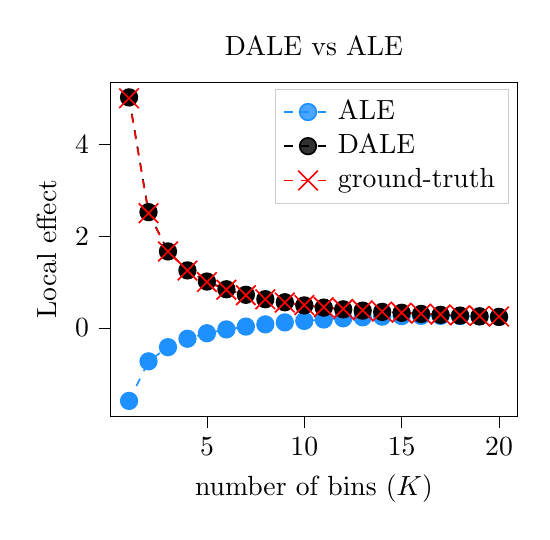
\begin{tikzpicture}

\definecolor{darkgray176}{RGB}{176,176,176}
\definecolor{dodgerblue}{RGB}{30,144,255}
\definecolor{lightgray204}{RGB}{204,204,204}

\begin{axis}[
legend cell align={left},
legend style={fill opacity=0.8, draw opacity=1, text opacity=1, draw=lightgray204},
tick align=outside,
tick pos=left,
title={DALE vs ALE},
x grid style={darkgray176},
xlabel={number of bins \(\displaystyle (K)\)},
xmin=0.0499999999999999, xmax=20.95,
xtick style={color=black},
y grid style={darkgray176},
ylabel={Local effect},
ymin=-1.9158582242841, ymax=5.35027643439794,
ytick style={color=black}
]
\addplot [semithick, dodgerblue, dashed, mark=*, mark size=3, mark options={solid}]
table {%
1 -1.58557937616219
2 -0.724469128659219
3 -0.415970121031068
4 -0.232936150463663
5 -0.11325432870959
6 -0.02954530629491
7 0.0314157941118509
8 0.0799920748845464
9 0.122926085482714
10 0.155053447821085
11 0.186088568383995
12 0.211864987771331
13 0.233108878251814
14 0.247869171569635
15 0.259566596177554
16 0.264108921400541
17 0.263569771086526
18 0.260892620884744
19 0.252751953555994
20 0.242460730712491
};
\addlegendentry{ALE}
\addplot [semithick, black, dashed, mark=*, mark size=3, mark options={solid}]
table {%
1 5.01999758627603
2 2.52286238913594
3 1.66707743267251
4 1.25440995432319
5 1.01184271234757
6 0.843722016967248
7 0.72371907999776
8 0.627936897660279
9 0.561288325580339
10 0.492398374084428
11 0.444051023514039
12 0.4070407257714
13 0.379038857924861
14 0.351678147881759
15 0.331857705495926
16 0.307844113455479
17 0.286910008925387
18 0.270908782811331
19 0.254748495290572
20 0.24246073071272
};
\addlegendentry{DALE}
\addplot [semithick, red, dashed, mark=x, mark size=5, mark options={solid}]
table {%
1 5
2 2.5
3 1.66666666666667
4 1.25
5 1
6 0.833333333333333
7 0.714285714285714
8 0.625
9 0.555555555555556
10 0.5
11 0.454545454545455
12 0.416666666666667
13 0.384615384615385
14 0.357142857142857
15 0.333333333333333
16 0.3125
17 0.294117647058824
18 0.277777777777778
19 0.263157894736842
20 0.25
};
\addlegendentry{ground-truth}
\end{axis}

\end{tikzpicture}
}
  \caption[Example comparison]{(Left) The black-box function \(f\) of
    Section~\ref{sec:4-3-robustness}. (Right) Estimation of the bin
    effect of the first bin for DALE and ALE, for varying number of
    bins \(K\).}
  \label{fig:example-different-bins}
\end{figure}


\subsection{Bias and variance}
\label{sec:4-4-std}
Let a finite dataset of samples \(\mathcal{S}\), drawn independently
and identically distributed (i.i.d) from the data generating
distribution of \(\mathcal{X}\). DALE computes the accumulated local
effect (Eq.~\eqref{eq:ALE}), using the approximation in
(Eq.~\eqref{eq:DALE}). The expected value of the approximation across
different datasets is

\begin{equation}
  \mathbb{E}_{\mathcal{S}}[\dale(x)] =
  \Delta x\sum_{k=1}^{k_x}\mathbb{E}_{\mathcal{S}}[\frac{1}{|\mathcal{S}_k|}\sum_{i:\xb^i \in
      \mathcal{S}_k} f_s(\xb^i)]
  \label{eq:bias_dale}
\end{equation}

\noindent
Notice also that for the values of \(x\) at the end of bin \(k_x\),
Eq.~\eqref{eq:ALE} can be rewritten as (after omitting the constant
\(c\))
\begin{equation}
  f_{\mathtt{ALE}}(x) = \sum_{k = 1}^{k_x}\int_{x_{k-1}}^{x_k}
    \mathbb{E}_{\Xcb|\mathcal{X}_s=z}[f_s(\xb)] \partial z
    \label{eq:bias_ale_1}
\end{equation}
where \(x_0=x_{s, min}\) and \(x_i\), \(i=1, \dotsc, k_x\) are the bin limits.

\noindent
If we assume that each bin is sufficiently small such that \(f_s(\xb)\) does
not depend on \(x_s\) (i.e., \(f(x)\) is linear wrt \(x_s\)) within the bin, then
Eq. \eqref{eq:bias_ale_1} becomes
\begin{equation}
  f_{\mathtt{ALE}}(x) = \sum_{k = 1}^{k_x}\mathbb{E}_{\Xcb|\mathcal{X}_s \in
    \mathcal{S}_k}[f_s(\xb)]\int_{x_{k-1}}^{x_k} \partial z
  = \Delta x\sum_{k=1}^{k_x}\mathbb{E}_{\mathcal{X} \in \mathcal{S}_k}[f_s(\xb)]
    \label{eq:bias_ale_2}
\end{equation}

\noindent
From Eqs. \eqref{eq:bias_dale} and \eqref{eq:bias_ale_2} we have
\begin{multline}
    \mathbb{E}_{\mathcal{S}}[\dale]  - f_{\mathtt{ALE}}(x) =
    \Delta x\sum_{k=1}^{k_x}\mathbb{E}_{\mathcal{S}}[\frac{1}{|\mathcal{S}_k|}\sum_{k:\xb^k \in
        \mathcal{S}_k} f_s(\xb^k)] - \\
    \Delta x\sum_{k=1}^{k_x}\mathbb{E}_{\mathcal{X}\in \mathcal{S}_k}[f_s(\xb)] =
  \Delta x\sum_{k=1}^{k_x}\left(\mathbb{E}_{\mathcal{S}}[\hat{\mu}_k^s] - \mu_k^s\right) = 0
\end{multline}
since the expected value of the sample mean is an unbiased estimator
of \(\mu_k^s\). As a result, under the condition of linearity wrt
\(x_s\) within the bin, DALE is an unbiased estimator of the feature
effect. If this assumption is violated (e.g., large bin size or highly
nonlinear function), then this approach may introduce bias. The
variance of the estimator is given\footnote{We show that in the
  supporting material.} by
\( \mathrm{Var}[\hat{\mu}_k^s] =
\dfrac{(\sigma_k^s)^2}{|\mathcal{S}_k|} \), where \((\sigma_k^s)^2\)
is the variance of \(f_s\) within the bin. Furthermore, since the
samples \(\xb^i\) are independent, \(\hat{\mu}_k^s\) for
\(k=1,\dotsc,k_x\) are also independent. The variance of the
estimation can then be approximated as
%
\begin{equation}
  \mathrm{Var}[\dale(x)] = (\Delta x)^2\sum_k^{k_x} \mathrm{Var} [\hat{\mu}_k^s]
  = (\Delta x)^2 \sum_k^{k_x}  \dfrac{(\sigma_k^s)^2}{|\mathcal{S}_k|} \approx
  (\Delta x)^2 \sum_k^{k_x}  \dfrac{(\hat{\sigma}_k^s)^2}{|\mathcal{S}_k|}
  \label{eq:DALE-var}
\end{equation}
%
where \((\hat{\sigma}_k^s)^2\) is the sample variance within bin
\(k\). Equation~\eqref{eq:DALE-var} allows the calculation of the
standard error for the DALE approximation.


% \subsection{Limitations of DALE}
% \label{sec:3-5-limitations}
% \input{./chapters/3-5-limitations.tex}

\section{Experiments}

This section presents the experimental evaluation of DALE using two
synthetic and one real dataset. The experiments aim to compare DALE
(\(\dale\)) with ALE approximation
(\(\hat{f}_{\mathtt{ALE}}\)) from the perspectives of both efficiency
and accuracy.

\paragraph{Metrics.} For evaluating the efficiency of the
approximations we measure the execution times (in seconds). For
evaluating the accuracy we use: (a) qualitative comparison of the
feature effect plots and (b) the Normalized Mean Squared Error which
is defined as
\(\text{NMSE}_{\mathtt{<approx>}} = \frac{\E[(\ale -
  f_{\mathtt{<approx>}})^2]}{\text{Var}[\ale]}\).

\paragraph{Synthetic Datasets.} The first synthetic dataset (Case 1) is designed
to compare the approximations in terms of efficiency. For this reason,
we generate design matrices \(\mathbf{X}\) of varying dimensionality
\(D\) and number of instances \(N\). The second synthetic dataset
(Case 2) is designed to compare the approximations in terms of
accuracy. We define a data generating distribution \(\mathcal{X}\) and
a black box function \(f\) with known forms for being able to directly
compute the ground-truth ALE from Eq.~\eqref{eq:ALE}. Both
\(\mathcal{X}\) and \(f\) are designed to amplify the effect of OOD
sampling.

\paragraph{Real Dataset} We choose the Bike-Sharing dataset for two
reasons. Firstly, it is the dataset utilized in the original ALE
paper, so it is a proper choice for unbiased comparisons. Secondly, we
wanted a dataset with enough training points to approximate the
feature effect accurately, since the ground-truth is not
available. Therefore, we want to check that \(\dale\) and
\(\hat{f}_{\mathtt{ALE}}\) provide similar effects using dense
bins. We also evaluate the accuracy of both methods behave when using
larger bins.

\subsection{Synthetic Datasets}
\label{sec:5-1-artificial-experiments}
\subsubsection{Case 1 - Efficiency comparison}
\label{sec:case-1}

In this example, we evaluate the efficiency of the two approximations,
\(\dale\) and \(\hat{f}_{\mathtt{ALE}}\), through the
execution times. We want to compare how both approximations perform in
terms of the dimensionality of the problem (\(D\)), the dataset size
(\(N\)) and the size of the model \(L\). In each experiment we
generate a design-matrix \( \mathbf{X} \), by drawing \( N \cdot D \)
samples from a standard normal distribution. The black-box function
\(f \) is a fully-connected neural network with \(L\) hidden layers of
\( 1024 \) units each. All experiments are done using \(K=100\). We
want to clarify that the value of \(K\) plays almost no role in the
execution times.

In Figure~\Ref{fig:case-1-plots-1}, we directly compare
\(\dale\) and \(\hat{f}_{\mathtt{ALE}}\) in two different
setups: in Figure~\Ref{fig:case-1-plots-1}(Left), we use a light setup
of \(N=10^3\) examples and a model of \(L=2\) layers, whereas in
Figure~\Ref{fig:case-1-plots-1}(Right), a heavier setup with
\(N=10^5\) and \(L=6\). We observe that in both cases, DALE executes
in near-constant time independently of \(D\), while ALE scales
linearly with wrt \(D\), confirming our claims of
Section~\ref{sec:4-2-computational}. The difference in the execution
time reaches significant levels from a relatively small
dimensionality. In the heavy setup, ALE needs almost a minute for
\(D=20\), three minutes for \(D=50\), and 15 minutes for \(D=100\). In
all these cases, DALE executes in a few seconds. Another critical
remark is that DALE's execution time is almost identical to the
computation of the Jacobian \( \Jac \), which is benefited by
automatic differentiation. Hence, we confirm that the overhead of
performing steps 3-5 of Algorithm~\ref{alg:dale} is a small fraction
of the total execution time. Another consequence of this remark is
that we can test many different bin sizes with near-zero computational
cost.

In Figure~\Ref{fig:case-1-plots-2}, we rigorously quantify to what
extent the dataset size \(N\) and the model size \(L\) affect both
methods. In Figures~\Ref{fig:case-1-plots-2}(a) and
~\Ref{fig:case-1-plots-2}(c), we confirm that both \(N\) and \(L\)
have crucial impact in ALE's execution times. Therefore, for a big
dataset and a heavy model \(f\), ALE's execution time quickly reaches
prohibitive levels. In contrast, in
Figures~\Ref{fig:case-1-plots-2}(b) and
Figures~\Ref{fig:case-1-plots-2}(d), DALE is negligibly affected by
these parameters. In the figures, we restrict the experiment to cases
up to 100-dimensional input for illustration purposes. The same trend
continues for an arbitrary number of dimensions. DALE can scale
efficiently to any dimensionality as long as we have enough resources
to store the dataset, evaluate the prediction model \(f\) and apply
the gradients \(\nabla_{\xb}f\).

\begin{figure}[h]
  \centering
  \resizebox{.4\columnwidth}{!}{% This file was created with tikzplotlib v0.10.1.
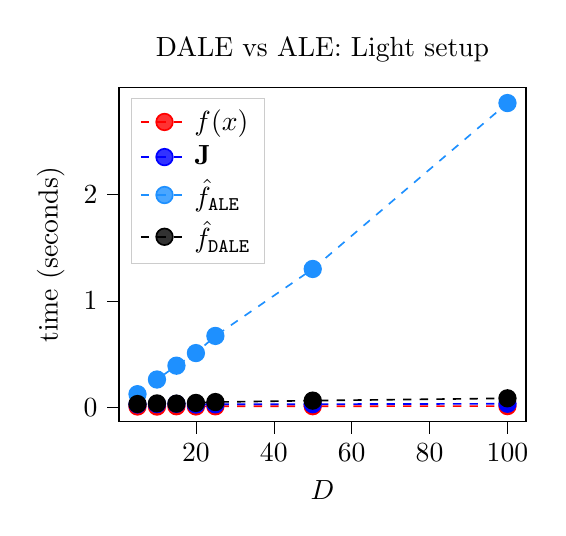
\begin{tikzpicture}

\definecolor{darkgray176}{RGB}{176,176,176}
\definecolor{dodgerblue}{RGB}{30,144,255}
\definecolor{lightgray204}{RGB}{204,204,204}

\begin{axis}[
legend cell align={left},
legend style={
  fill opacity=0.8,
  draw opacity=1,
  text opacity=1,
  at={(0.03,0.97)},
  anchor=north west,
  draw=lightgray204
},
tick align=outside,
tick pos=left,
title={DALE vs ALE: Light setup},
x grid style={darkgray176},
xlabel={\(\displaystyle D\)},
xmin=0.25, xmax=104.75,
xtick style={color=black},
y grid style={darkgray176},
ylabel={time (seconds)},
ymin=-0.131140862051234, ymax=2.99683744304994,
ytick style={color=black}
]
\addplot [semithick, red, dashed, mark=*, mark size=3, mark options={solid}]
table {%
5 0.0118236541748047
10 0.0110399723052979
15 0.0141679048538208
20 0.0121772289276123
25 0.0137112140655518
50 0.0146358013153076
100 0.0155208110809326
};
\addlegendentry{$f(x)$}
\addplot [semithick, blue, dashed, mark=*, mark size=3, mark options={solid}]
table {%
5 0.0307250022888184
10 0.0338666439056396
15 0.0361539125442505
20 0.0303496122360229
25 0.0321464538574219
50 0.0336906909942627
100 0.0372809171676636
};
\addlegendentry{$\mathbf{J}$}
\addplot [semithick, dodgerblue, dashed, mark=*, mark size=3, mark options={solid}]
table {%
5 0.127132534980774
10 0.264535903930664
15 0.394240617752075
20 0.51231861114502
25 0.672989368438721
50 1.30030632019043
100 2.85465669631958
};
\addlegendentry{$\hat{f}_{\mathtt{ALE}}$}
\addplot [semithick, black, dashed, mark=*, mark size=3, mark options={solid}]
table {%
5 0.0349620580673218
10 0.0408366918563843
15 0.0389609336853027
20 0.0452711582183838
25 0.0536262989044189
50 0.0669845342636108
100 0.0886013507843018
};
\addlegendentry{$\hat{f}_{\mathtt{DALE}}$}
\end{axis}

\end{tikzpicture}
}
  \resizebox{.43\columnwidth}{!}{% This file was created with tikzplotlib v0.10.1.
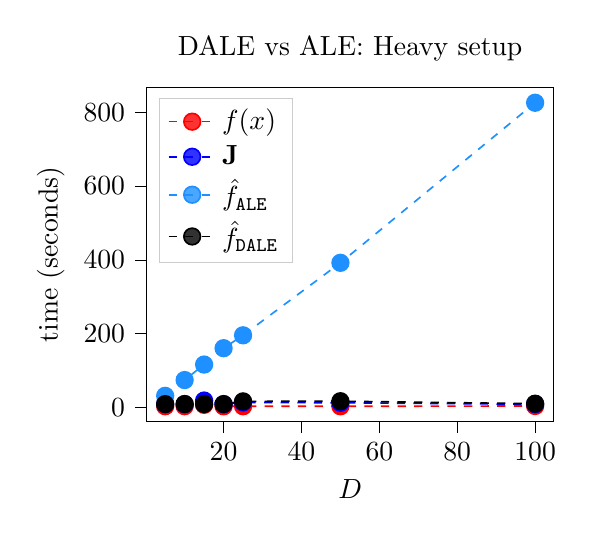
\begin{tikzpicture}

\definecolor{darkgray176}{RGB}{176,176,176}
\definecolor{dodgerblue}{RGB}{30,144,255}
\definecolor{lightgray204}{RGB}{204,204,204}

\begin{axis}[
legend cell align={left},
legend style={
  fill opacity=0.8,
  draw opacity=1,
  text opacity=1,
  at={(0.03,0.97)},
  anchor=north west,
  draw=lightgray204
},
tick align=outside,
tick pos=left,
title={DALE vs ALE: Heavy setup},
x grid style={darkgray176},
xlabel={\(\displaystyle D\)},
xmin=0.25, xmax=104.75,
xtick style={color=black},
y grid style={darkgray176},
ylabel={time (seconds)},
ymin=-38.1810145603003, ymax=867.056094992299,
ytick style={color=black}
]
\addplot [semithick, red, dashed, mark=*, mark size=3, mark options={solid}]
table {%
5 3.13364505767822
10 3.24496150016785
15 6.86045789718628
20 2.96612668037415
25 3.05197858810425
50 3.02510833740234
100 3.71672296524048
};
\addlegendentry{$f(x)$}
\addplot [semithick, blue, dashed, mark=*, mark size=3, mark options={solid}]
table {%
5 8.88222980499268
10 8.82908821105957
15 18.4925575256348
20 8.51719951629639
25 13.5228071212769
50 12.4858655929565
100 8.59451198577881
};
\addlegendentry{$\mathbf{J}$}
\addplot [semithick, dodgerblue, dashed, mark=*, mark size=3, mark options={solid}]
table {%
5 31.310697555542
10 74.1438674926758
15 116.133689880371
20 160.465118408203
25 195.409912109375
50 391.950622558594
100 825.908935546875
};
\addlegendentry{$\hat{f}_{\mathtt{ALE}}$}
\addplot [semithick, black, dashed, mark=*, mark size=3, mark options={solid}]
table {%
5 8.83595371246338
10 9.03882694244385
15 9.21370220184326
20 8.9499044418335
25 16.3313121795654
50 16.7110271453857
100 10.0340776443481
};
\addlegendentry{$\hat{f}_{\mathtt{DALE}}$}
\end{axis}

\end{tikzpicture}
}
  \caption[Case-1-fig-1]{Case 1. Comparison of the execution time of DALE
    and ALE in two setups: (Left) Light setup; \(N=10^3, L=2\).
    (Right) Light setup; \(N=10^5, L=6\)}
  \label{fig:case-1-plots-1}
\end{figure}

\begin{figure}[h]
  \centering
  \resizebox{.23\columnwidth}{!}{% This file was created with tikzplotlib v0.10.1.
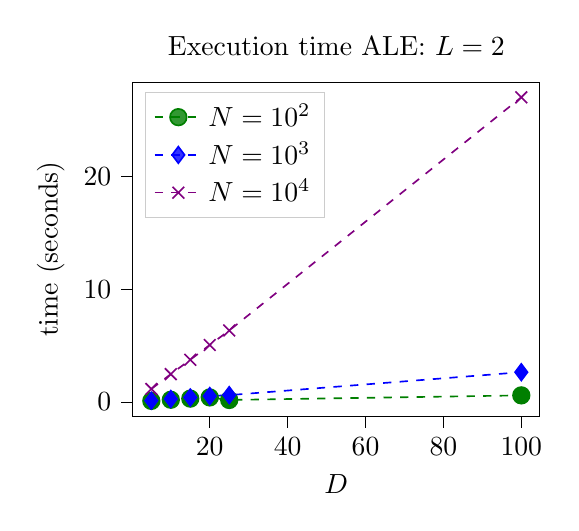
\begin{tikzpicture}

\definecolor{darkgray176}{RGB}{176,176,176}
\definecolor{green01270}{RGB}{0,127,0}
\definecolor{lightgray204}{RGB}{204,204,204}
\definecolor{purple}{RGB}{128,0,128}

\begin{axis}[
legend cell align={left},
legend style={
  fill opacity=0.8,
  draw opacity=1,
  text opacity=1,
  at={(0.03,0.97)},
  anchor=north west,
  draw=lightgray204
},
tick align=outside,
tick pos=left,
title={Execution time ALE: \(\displaystyle L=2\)},
x grid style={darkgray176},
xlabel={\(\displaystyle D\)},
xmin=0.25, xmax=104.75,
xtick style={color=black},
y grid style={darkgray176},
ylabel={time (seconds)},
ymin=-1.24482673455045, ymax=28.3690538155494,
ytick style={color=black}
]
\addplot [semithick, green01270, dashed, mark=*, mark size=3, mark options={solid}]
table {%
5 0.101258754730225
10 0.202309727668762
15 0.302774310112
20 0.410390853881836
25 0.183210730552673
100 0.592442154884338
};
\addlegendentry{$N=10^2$}
\addplot [semithick, blue, dashed, mark=diamond*, mark size=3, mark options={solid}]
table {%
5 0.122078418731689
10 0.273244619369507
15 0.406428098678589
20 0.527456998825073
25 0.613609552383423
100 2.64824438095093
};
\addlegendentry{$N=10^3$}
\addplot [semithick, purple, dashed, mark=x, mark size=3, mark options={solid}]
table {%
5 1.15858960151672
10 2.47470235824585
15 3.75058650970459
20 5.05907726287842
25 6.34863948822021
100 27.0229682922363
};
\addlegendentry{$N=10^4$}
\end{axis}

\end{tikzpicture}
}
  \resizebox{.23\columnwidth}{!}{% This file was created with tikzplotlib v0.10.1.
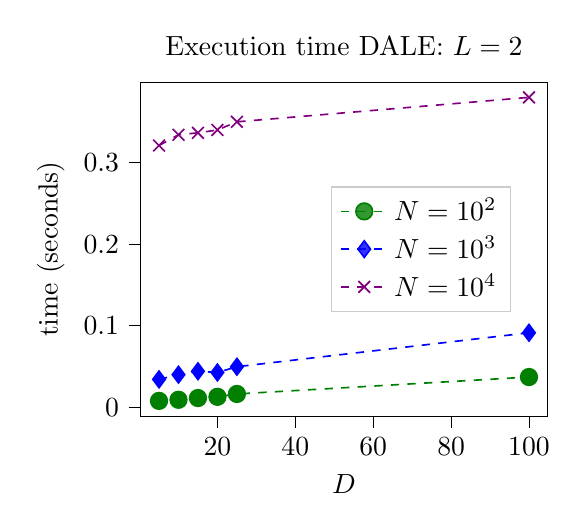
\begin{tikzpicture}

\definecolor{darkgray176}{RGB}{176,176,176}
\definecolor{green01270}{RGB}{0,127,0}
\definecolor{lightgray204}{RGB}{204,204,204}
\definecolor{purple}{RGB}{128,0,128}

\begin{axis}[
legend cell align={left},
legend style={
  fill opacity=0.8,
  draw opacity=1,
  text opacity=1,
  at={(0.91,0.5)},
  anchor=east,
  draw=lightgray204
},
tick align=outside,
tick pos=left,
title={Execution time DALE: \(\displaystyle L=2\)},
x grid style={darkgray176},
xlabel={\(\displaystyle D\)},
xmin=0.25, xmax=104.75,
xtick style={color=black},
y grid style={darkgray176},
ylabel={time (seconds)},
ymin=-0.0109329749522149, ymax=0.398615855950105,
ytick style={color=black}
]
\addplot [semithick, green01270, dashed, mark=*, mark size=3, mark options={solid}]
table {%
5 0.0076829195022583
10 0.00905656814575195
15 0.0112016201019287
20 0.0126841068267822
25 0.0161861181259155
100 0.0369504690170288
};
\addlegendentry{$N=10^2$}
\addplot [semithick, blue, dashed, mark=diamond*, mark size=3, mark options={solid}]
table {%
5 0.0340769290924072
10 0.0398837327957153
15 0.0440537929534912
20 0.0425540208816528
25 0.0495928525924683
100 0.0912438631057739
};
\addlegendentry{$N=10^3$}
\addplot [semithick, purple, dashed, mark=x, mark size=3, mark options={solid}]
table {%
5 0.320958256721497
10 0.334092974662781
15 0.33648693561554
20 0.340000033378601
25 0.350000023841858
100 0.379999995231628
};
\addlegendentry{$N=10^4$}
\end{axis}

\end{tikzpicture}
}
  \resizebox{.23\columnwidth}{!}{% This file was created with tikzplotlib v0.10.1.
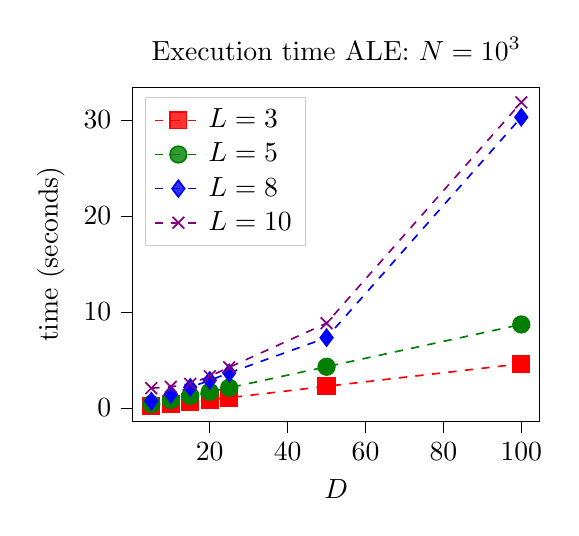
\begin{tikzpicture}

\definecolor{darkgray176}{RGB}{176,176,176}
\definecolor{green01270}{RGB}{0,127,0}
\definecolor{lightgray204}{RGB}{204,204,204}
\definecolor{purple}{RGB}{128,0,128}

\begin{axis}[
legend cell align={left},
legend style={
  fill opacity=0.8,
  draw opacity=1,
  text opacity=1,
  at={(0.03,0.97)},
  anchor=north west,
  draw=lightgray204
},
tick align=outside,
tick pos=left,
title={Execution time ALE: \(\displaystyle N=10^3\)},
x grid style={darkgray176},
xlabel={\(\displaystyle D\)},
xmin=0.25, xmax=104.75,
xtick style={color=black},
y grid style={darkgray176},
ylabel={time (seconds)},
ymin=-1.36616255235276, ymax=33.4035613893502,
ytick style={color=black}
]
\addplot [semithick, red, dashed, mark=square*, mark size=3, mark options={solid}]
table {%
5 0.214279413223267
10 0.445428252220154
15 0.637093186378479
20 0.876859426498413
25 1.06718361377716
50 2.25691056251526
100 4.60215711593628
};
\addlegendentry{$L=3$}
\addplot [semithick, green01270, dashed, mark=*, mark size=3, mark options={solid}]
table {%
5 0.408349752426147
10 0.824460029602051
15 1.26256990432739
20 1.68054091930389
25 2.10548663139343
50 4.29162120819092
100 8.69534683227539
};
\addlegendentry{$L=5$}
\addplot [semithick, blue, dashed, mark=diamond*, mark size=3, mark options={solid}]
table {%
5 0.71037769317627
10 1.42690515518188
15 2.14693737030029
20 2.87370538711548
25 3.65433740615845
50 7.31730794906616
100 30.2758731842041
};
\addlegendentry{$L=8$}
\addplot [semithick, purple, dashed, mark=x, mark size=3, mark options={solid}]
table {%
5 2.06213808059692
10 2.20000004768372
15 2.5
20 3.30623149871826
25 4.2340202331543
50 8.82898712158203
100 31.8231201171875
};
\addlegendentry{$L=10$}
\end{axis}

\end{tikzpicture}
}
  \resizebox{.23\columnwidth}{!}{% This file was created with tikzplotlib v0.10.1.
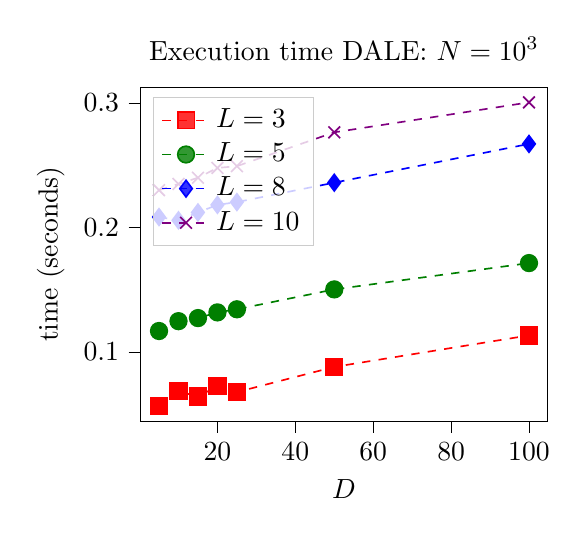
\begin{tikzpicture}

\definecolor{darkgray176}{RGB}{176,176,176}
\definecolor{green01270}{RGB}{0,127,0}
\definecolor{lightgray204}{RGB}{204,204,204}
\definecolor{purple}{RGB}{128,0,128}

\begin{axis}[
legend cell align={left},
legend style={
  fill opacity=0.8,
  draw opacity=1,
  text opacity=1,
  at={(0.03,0.97)},
  anchor=north west,
  draw=lightgray204
},
tick align=outside,
tick pos=left,
title={Execution time DALE: \(\displaystyle N=10^3\)},
x grid style={darkgray176},
xlabel={\(\displaystyle D\)},
xmin=0.25, xmax=104.75,
xtick style={color=black},
y grid style={darkgray176},
ylabel={time (seconds)},
ymin=0.0445653210494129, ymax=0.312711131950527,
ytick style={color=black}
]
\addplot [semithick, red, dashed, mark=square*, mark size=3, mark options={solid}]
table {%
5 0.0567537546157837
10 0.0685902833938599
15 0.0642098188400269
20 0.0725626945495605
25 0.0678497552871704
50 0.088062047958374
100 0.113367915153503
};
\addlegendentry{$L=3$}
\addplot [semithick, green01270, dashed, mark=*, mark size=3, mark options={solid}]
table {%
5 0.116896510124207
10 0.124809384346008
15 0.127277135848999
20 0.131840586662292
25 0.134345889091492
50 0.150314569473267
100 0.171453237533569
};
\addlegendentry{$L=5$}
\addplot [semithick, blue, dashed, mark=diamond*, mark size=3, mark options={solid}]
table {%
5 0.208409428596497
10 0.205777525901794
15 0.212119460105896
20 0.218204021453857
25 0.220425486564636
50 0.236039161682129
100 0.267152309417725
};
\addlegendentry{$L=8$}
\addplot [semithick, purple, dashed, mark=x, mark size=3, mark options={solid}]
table {%
5 0.230000019073486
10 0.235000014305115
15 0.240000009536743
20 0.247859835624695
25 0.249285697937012
50 0.276461362838745
100 0.300522685050964
};
\addlegendentry{$L=10$}
\end{axis}

\end{tikzpicture}
}
  \caption[Case-1-fig-2]{Case 1. Measurements of the execution time wrt dimensionality \(D\):
    (a) \(\hat{f}_{\mathtt{ALE}}\) for \(L = 2\), and many dataset sizes \(N\)
    (b) \(\hat{f}_{\mathtt{ALE}}\) for \(N = 10^3\), and many model sizes \(L\)
    (c) \(\dale\) for \(L = 2\), and many dataset sizes \(N\)
    (d) \(\dale\) for \(N = 10^3\), and many model sizes \(L\)
  }
  \label{fig:case-1-plots-2}
\end{figure}


\subsubsection{Case 2 - Accuracy Comparison}
\label{sec:example2}

In this example, we evaluate the accuracy of the two approximations,
\(\dale\) and \(\hat{f}_{\mathtt{ALE}}\), in a synthetic
dataset where the ground truth ALE is accessible. As discussed in
Section~\ref{sec:4-3-robustness}, ALE approximation is vulnerable to
OOD sampling when the bins are wide, or equivalently, the number of
bins \(K\) is small. We want to compare how both approximations behave
in a case where the local effect is noisy.
%
We design an experiment where we know the black-box function and the
data generating distribution. The black-box function
\(f:\R^3 \rightarrow \R\) is split in three parts to amplify the
effect of OOD sampling. It includes a mild term
\( f_0(x) = x_1x_2 + x_1x_3 \) in the region
\( 0 \leq |x_1 - x_2| < \tau \) and then a quadratic term
\(g(x) = \alpha ((x_1 - x_2)^2 - \tau^2)\) is added(subtracted)
over(under) the region, i.e.:

\begin{equation} \label{eq:example-2-mapping}
  f(\mathbf{x}) =
  \begin{cases}
    f_0(x) & , 0 \leq |x_1 - x_2|  < \tau \\
    f_0(x) - g(x) & , \tau \leq |x_1 - x_2|  \\
    f_0(x) + g(x) & , \tau \leq - |x_1 - x_2|  \\
  \end{cases}
\end{equation}

\noindent
%
The data points \(X^i = (x_1^i, x_2^i, x_3^i)\) are generated as
follows; \(x_1^i \) are clustered around the points
\(\{1.5, 3, 5, 7, 8.5\}\),
\(x_2^i \sim \mathcal{N}(\mu=x_1, \sigma_2=0.1) \) and
\(x_3^i \sim \mathcal{N}(\mu=0, \sigma_3^2=10) \). In
Figure~\ref{fig:example-2-samples}(a), we illustrate \(f(\xb)\) for
\(x_3=0\), as well as the generated data points. In this example, the
local effect of \(x_1\) is
\(\frac{\partial f}{\partial x_1} = x_2 + x_3\). Due to the noisy
nature of \(x_3\), both ALE and DALE need a large number of sample for
robust estimation. Therefore, we need to lower the number of bins
\(K\). As will be shown below, both ALE and DALE fail to approximate
the feature effect for high \(K\). On the other hand, when using a
lower \(K\), ALE approximation fails due to OOD sampling, while DALE
manages to accurately approximate the feature effect.

In Figure~\ref{fig:example-2-samples}(b) and
Figure~\ref{fig:example-2-samples}(c), we observe the estimated
effects for \(K=50\) and \(K=5\). In
Figure~\ref{fig:example-2-samples}(b), \((K=50)\) the approximations
converge to the same estimated effect which is inaccurate due to many
noisy artifacts. In Figure~\ref{fig:example-2-samples}(c), \((K=5)\)
we observe that for small \(K\), DALE approximates the ground-truth
effect well, whereas ALE fails due to OOD
sampling. Table~\ref{tab:case-2-accuracy} provides the NMSE of both
approximation for varying number of bins \(K\). We observe that DALE
consistently provides accurate estimations (NMSE \(\leq 0.1\)) for all
small \(K\) values.

The experiments helps us confirm that when \(K \) increases, both
approximations are based on a limited number of samples, and are
vulnerable to noise. When \(K\) decreases, DALE lowers the resolution
but provides more robust estimations. In contrast, ALE is vulnerable
to OOD sampling.

\begin{table}
  \centering
  \caption{Case 2. Evaluation of the NMSE between the approximations and the ground truth. Blue color indicates the values that are below \(0.1\).}
  \label{tab:case-2-accuracy}
  \begin{tabular}{c|c|c|c|c|c|c|c|c|c}
    \multicolumn{10}{c}{Accuracy on the Synthetic Dataset (Case 2)} \\
    \hline \hline
    & & \multicolumn{8}{|c}{Number of bins} \\
    \hline
    & & 1 & 2 & 3 & 4 & 5 & 10 & 20 & 40 \\
    \hline
    \hline
    \multirow{2}{*}{\(\mathtt{NMSE}\)} & \(\dale\) & \textcolor{blue}{0.10} & \textcolor{blue}{0.03} & \textcolor{blue}{0.09} & \textcolor{blue}{0.02} & \textcolor{blue}{0.02} & 0.82 & 0.24 & 0.38\\
    & \(\alep\) & 100.42 & 22.09 & 4.97 & 2.81 & 0.78 & 1.49 & 0.34 & 0.39 \\
    \hline
  \end{tabular}
\end{table}


\begin{figure}[h]
  \begin{center}
    \resizebox{.33\columnwidth}{!}{% This file was created with tikzplotlib v0.10.1.
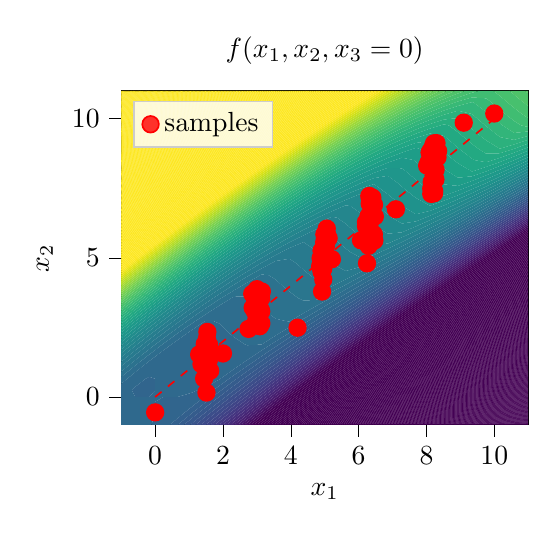
\begin{tikzpicture}

\definecolor{darkcyan30153138}{RGB}{30,153,138}
\definecolor{darkcyan30157136}{RGB}{30,157,136}
\definecolor{darkcyan31146140}{RGB}{31,146,140}
\definecolor{darkcyan31150139}{RGB}{31,150,139}
\definecolor{darkcyan31162134}{RGB}{31,162,134}
\definecolor{darkcyan33141140}{RGB}{33,141,140}
\definecolor{darkcyan34137141}{RGB}{34,137,141}
\definecolor{darkcyan36134141}{RGB}{36,134,141}
\definecolor{darkcyan37130142}{RGB}{37,130,142}
\definecolor{darkcyan39125142}{RGB}{39,125,142}
\definecolor{darkgray176}{RGB}{176,176,176}
\definecolor{darkslateblue47105141}{RGB}{47,105,141}
\definecolor{darkslateblue49101141}{RGB}{49,101,141}
\definecolor{darkslateblue5196141}{RGB}{51,96,141}
\definecolor{darkslateblue5392140}{RGB}{53,92,140}
\definecolor{darkslateblue5588140}{RGB}{55,88,140}
\definecolor{darkslateblue5784139}{RGB}{57,84,139}
\definecolor{darkslateblue6078138}{RGB}{60,78,138}
\definecolor{darkslateblue6174137}{RGB}{61,74,137}
\definecolor{darkslateblue6369135}{RGB}{63,69,135}
\definecolor{darkslateblue6565134}{RGB}{65,65,134}
\definecolor{darkslateblue6759131}{RGB}{67,59,131}
\definecolor{darkslateblue6954129}{RGB}{69,54,129}
\definecolor{darkslateblue7049126}{RGB}{70,49,126}
\definecolor{darkslateblue7138118}{RGB}{71,38,118}
\definecolor{darkslateblue7144123}{RGB}{71,44,123}
\definecolor{gold21822624}{RGB}{218,226,24}
\definecolor{gold22822724}{RGB}{228,227,24}
\definecolor{gold23822927}{RGB}{238,229,27}
\definecolor{gold24823033}{RGB}{248,230,33}
\definecolor{gold25323136}{RGB}{253,231,36}
\definecolor{greenyellow19422334}{RGB}{194,223,34}
\definecolor{greenyellow20522429}{RGB}{205,224,29}
\definecolor{indigo68184}{RGB}{68,1,84}
\definecolor{indigo68387}{RGB}{68,3,87}
\definecolor{indigo70992}{RGB}{70,9,92}
\definecolor{indigo711598}{RGB}{71,15,98}
\definecolor{indigo7121103}{RGB}{71,21,103}
\definecolor{indigo7228110}{RGB}{72,28,110}
\definecolor{indigo7233114}{RGB}{72,33,114}
\definecolor{lightgray204}{RGB}{204,204,204}
\definecolor{mediumseagreen10720589}{RGB}{107,205,89}
\definecolor{mediumseagreen33166133}{RGB}{33,166,133}
\definecolor{mediumseagreen35169130}{RGB}{35,169,130}
\definecolor{mediumseagreen40174127}{RGB}{40,174,127}
\definecolor{mediumseagreen44177125}{RGB}{44,177,125}
\definecolor{mediumseagreen50181122}{RGB}{50,181,122}
\definecolor{mediumseagreen56185118}{RGB}{56,185,118}
\definecolor{mediumseagreen64189114}{RGB}{64,189,114}
\definecolor{mediumseagreen71192110}{RGB}{71,192,110}
\definecolor{mediumseagreen79195105}{RGB}{79,195,105}
\definecolor{mediumseagreen87198101}{RGB}{87,198,101}
\definecolor{mediumseagreen9820295}{RGB}{98,202,95}
\definecolor{steelblue46109142}{RGB}{46,109,142}
\definecolor{teal40122142}{RGB}{40,122,142}
\definecolor{teal42118142}{RGB}{42,118,142}
\definecolor{teal44114142}{RGB}{44,114,142}
\definecolor{yellowgreen11620884}{RGB}{116,208,84}
\definecolor{yellowgreen12621078}{RGB}{126,210,78}
\definecolor{yellowgreen13921370}{RGB}{139,213,70}
\definecolor{yellowgreen14921563}{RGB}{149,215,63}
\definecolor{yellowgreen15921756}{RGB}{159,217,56}
\definecolor{yellowgreen17322048}{RGB}{173,220,48}
\definecolor{yellowgreen18322141}{RGB}{183,221,41}

\begin{axis}[
legend cell align={left},
legend style={
  fill opacity=0.8,
  draw opacity=1,
  text opacity=1,
  at={(0.03,0.97)},
  anchor=north west,
  draw=lightgray204
},
tick align=outside,
tick pos=left,
title={\(\displaystyle f(x_1, x_2, x_3=0)\)},
x grid style={darkgray176},
xlabel={\(\displaystyle x_1\)},
xmin=-1, xmax=11,
xtick style={color=black},
y grid style={darkgray176},
ylabel={\(\displaystyle x_2\)},
ymin=-1, ymax=11,
ytick style={color=black}
]
\addplot [draw=none, fill=indigo68184, forget plot]
table{%
x  y
11 -1
11 -0.977740356373605
10.9764002491177 -1
11 -1
};
\addplot [draw=none, fill=indigo68184, forget plot]
table{%
x  y
11 -0.977740356373605
11 -0.949347953788917
10.9462985260536 -1
10.9764002491177 -1
11 -0.977740356373605
};
\addplot [draw=none, fill=indigo68184, forget plot]
table{%
x  y
11 -0.949347953788917
11 -0.92095555120423
10.9161968029894 -1
10.9462985260536 -1
11 -0.949347953788917
};
\addplot [draw=none, fill=indigo68184, forget plot]
table{%
x  y
11 -0.92095555120423
11 -0.892563148619542
10.8860950799253 -1
10.9161968029894 -1
11 -0.92095555120423
};
\addplot [draw=none, fill=indigo68184, forget plot]
table{%
x  y
11 -0.892563148619542
11 -0.864170746034854
10.8559933568611 -1
10.8860950799253 -1
11 -0.892563148619542
};
\addplot [draw=none, fill=indigo68184, forget plot]
table{%
x  y
11 -0.864170746034854
11 -0.835778343450167
10.825891633797 -1
10.8559933568611 -1
11 -0.864170746034854
};
\addplot [draw=none, fill=indigo68184, forget plot]
table{%
x  y
11 -0.835778343450167
11 -0.807385940865479
10.7957899107328 -1
10.825891633797 -1
11 -0.835778343450167
};
\addplot [draw=none, fill=indigo68184, forget plot]
table{%
x  y
11 -0.807385940865479
11 -0.778993538280791
10.7656881876687 -1
10.7957899107328 -1
11 -0.807385940865479
};
\addplot [draw=none, fill=indigo68184, forget plot]
table{%
x  y
11 -0.778993538280791
11 -0.750601135696103
10.7355864646045 -1
10.7656881876687 -1
11 -0.778993538280791
};
\addplot [draw=none, fill=indigo68184, forget plot]
table{%
x  y
11 -0.750601135696103
11 -0.722208733111416
10.7054847415404 -1
10.7355864646045 -1
11 -0.750601135696103
};
\addplot [draw=none, fill=indigo68184, forget plot]
table{%
x  y
11 -0.722208733111416
11 -0.693816330526728
10.6753830184762 -1
10.7054847415404 -1
11 -0.722208733111416
};
\addplot [draw=none, fill=indigo68184, forget plot]
table{%
x  y
11 -0.693816330526728
11 -0.66542392794204
10.6452812954121 -1
10.6753830184762 -1
11 -0.693816330526728
};
\addplot [draw=none, fill=indigo68184, forget plot]
table{%
x  y
11 -0.66542392794204
11 -0.637031525357353
10.6151795723479 -1
10.6452812954121 -1
11 -0.66542392794204
};
\addplot [draw=none, fill=indigo68184, forget plot]
table{%
x  y
10.5862068965517 -1
10.6151795723479 -1
11 -0.637031525357353
11 -0.608639122772665
10.5862068965517 -0.998896159795077
10.5850370491244 -1
10.5862068965517 -1
};
\addplot [draw=none, fill=indigo68184, forget plot]
table{%
x  y
10.5862068965517 -0.998896159795077
11 -0.608639122772665
11 -0.586206896551724
11 -0.580043984891539
10.9934357082834 -0.586206896551724
10.5862068965517 -0.969466486565931
10.5538475460054 -1
10.5850370491244 -1
10.5862068965517 -0.998896159795077
};
\addplot [draw=none, fill=indigo68184, forget plot]
table{%
x  y
10.5862068965517 -0.969466486565931
10.9934357082834 -0.586206896551724
11 -0.580043984891539
11 -0.550685815221565
10.9621654904702 -0.586206896551724
10.5862068965517 -0.940036813336786
10.5226580428865 -1
10.5538475460054 -1
10.5862068965517 -0.969466486565931
};
\addplot [draw=none, fill=indigo68184, forget plot]
table{%
x  y
10.5862068965517 -0.940036813336786
10.9621654904702 -0.586206896551724
11 -0.550685815221565
11 -0.521327645551592
10.930895272657 -0.586206896551724
10.5862068965517 -0.91060714010764
10.4914685397675 -1
10.5226580428865 -1
10.5862068965517 -0.940036813336786
};
\addplot [draw=none, fill=indigo68184, forget plot]
table{%
x  y
10.5862068965517 -0.91060714010764
10.930895272657 -0.586206896551724
11 -0.521327645551592
11 -0.491969475881618
10.8996250548437 -0.586206896551724
10.5862068965517 -0.881177466878495
10.4602790366486 -1
10.4914685397675 -1
10.5862068965517 -0.91060714010764
};
\addplot [draw=none, fill=indigo68184, forget plot]
table{%
x  y
10.5862068965517 -0.881177466878495
10.8996250548437 -0.586206896551724
11 -0.491969475881618
11 -0.462611306211644
10.8683548370305 -0.586206896551724
10.5862068965517 -0.851747793649349
10.4290895335296 -1
10.4602790366486 -1
10.5862068965517 -0.881177466878495
};
\addplot [draw=none, fill=indigo68184, forget plot]
table{%
x  y
10.5862068965517 -0.851747793649349
10.8683548370305 -0.586206896551724
11 -0.462611306211644
11 -0.433253136541671
10.8370846192172 -0.586206896551724
10.5862068965517 -0.822318120420204
10.3979000304107 -1
10.4290895335296 -1
10.5862068965517 -0.851747793649349
};
\addplot [draw=none, fill=indigo68184, forget plot]
table{%
x  y
10.5862068965517 -0.822318120420204
10.8370846192172 -0.586206896551724
11 -0.433253136541671
11 -0.403894966871697
10.805814401404 -0.586206896551724
10.5862068965517 -0.792888447191058
10.3667105272917 -1
10.3979000304107 -1
10.5862068965517 -0.822318120420204
};
\addplot [draw=none, fill=indigo68184, forget plot]
table{%
x  y
10.5862068965517 -0.792888447191058
10.805814401404 -0.586206896551724
11 -0.403894966871697
11 -0.374536797201723
10.7745441835908 -0.586206896551724
10.5862068965517 -0.763458773961913
10.3355210241728 -1
10.3667105272917 -1
10.5862068965517 -0.792888447191058
};
\addplot [draw=none, fill=indigo68184, forget plot]
table{%
x  y
10.5862068965517 -0.763458773961913
10.7745441835908 -0.586206896551724
11 -0.374536797201723
11 -0.34517862753175
10.7432739657775 -0.586206896551724
10.5862068965517 -0.734029100732768
10.3043315210538 -1
10.3355210241728 -1
10.5862068965517 -0.763458773961913
};
\addplot [draw=none, fill=indigo68184, forget plot]
table{%
x  y
10.5862068965517 -0.734029100732768
10.7432739657775 -0.586206896551724
11 -0.34517862753175
11 -0.315820457861776
10.7120037479643 -0.586206896551724
10.5862068965517 -0.704599427503622
10.2731420179349 -1
10.3043315210538 -1
10.5862068965517 -0.734029100732768
};
\addplot [draw=none, fill=indigo68184, forget plot]
table{%
x  y
10.5862068965517 -0.704599427503622
10.7120037479643 -0.586206896551724
11 -0.315820457861776
11 -0.286462288191803
10.680733530151 -0.586206896551724
10.5862068965517 -0.675169754274477
10.2419525148159 -1
10.2731420179349 -1
10.5862068965517 -0.704599427503622
};
\addplot [draw=none, fill=indigo68184, forget plot]
table{%
x  y
10.5862068965517 -0.675169754274477
10.680733530151 -0.586206896551724
11 -0.286462288191803
11 -0.257104118521829
10.6494633123378 -0.586206896551724
10.5862068965517 -0.645740081045331
10.210763011697 -1
10.2419525148159 -1
10.5862068965517 -0.675169754274477
};
\addplot [draw=none, fill=indigo68184, forget plot]
table{%
x  y
10.5862068965517 -0.645740081045331
10.6494633123378 -0.586206896551724
11 -0.257104118521829
11 -0.227745948851855
10.6181930945246 -0.586206896551724
10.5862068965517 -0.616310407816186
10.179573508578 -1
10.210763011697 -1
10.5862068965517 -0.645740081045331
};
\addplot [draw=none, fill=indigo68184, forget plot]
table{%
x  y
10.1724137931034 -1
10.179573508578 -1
10.5862068965517 -0.616310407816186
10.6181930945246 -0.586206896551724
11 -0.227745948851855
11 -0.198387779181882
10.5869228767113 -0.586206896551724
10.5862068965517 -0.58688073458704
10.1724137931034 -0.976466298133849
10.1474830895197 -1
10.1724137931034 -1
};
\addplot [draw=none, fill=indigo68184, forget plot]
table{%
x  y
10.1724137931034 -0.976466298133849
10.5862068965517 -0.58688073458704
10.5869228767113 -0.586206896551724
11 -0.198387779181882
11 -0.172413793103448
11 -0.168910443122602
10.9962498355938 -0.172413793103448
10.5862068965517 -0.55643593626595
10.5545040547527 -0.586206896551724
10.1724137931034 -0.945920690381584
10.1151242410484 -1
10.1474830895197 -1
10.1724137931034 -0.976466298133849
};
\addplot [draw=none, fill=indigo68184, forget plot]
table{%
x  y
10.1724137931034 -0.945920690381584
10.5545040547527 -0.586206896551724
10.5862068965517 -0.55643593626595
10.9962498355938 -0.172413793103448
11 -0.168910443122602
11 -0.138518491749724
10.9637167415843 -0.172413793103448
10.5862068965517 -0.525967350428589
10.5220583174513 -0.586206896551724
10.1724137931034 -0.91537508262932
10.0827653925771 -1
10.1151242410484 -1
10.1724137931034 -0.945920690381584
};
\addplot [draw=none, fill=indigo68184, forget plot]
table{%
x  y
10.1724137931034 -0.91537508262932
10.5220583174513 -0.586206896551724
10.5862068965517 -0.525967350428589
10.9637167415843 -0.172413793103448
11 -0.138518491749724
11 -0.108126540376846
10.9311836475749 -0.172413793103448
10.5862068965517 -0.495498764591228
10.4896125801498 -0.586206896551724
10.1724137931034 -0.884829474877055
10.0504065441058 -1
10.0827653925771 -1
10.1724137931034 -0.91537508262932
};
\addplot [draw=none, fill=indigo68184, forget plot]
table{%
x  y
10.1724137931034 -0.884829474877055
10.4896125801498 -0.586206896551724
10.5862068965517 -0.495498764591228
10.9311836475749 -0.172413793103448
11 -0.108126540376846
11 -0.0777345890039684
10.8986505535655 -0.172413793103448
10.5862068965517 -0.465030178753868
10.4571668428484 -0.586206896551724
10.1724137931034 -0.85428386712479
10.0180476956344 -1
10.0504065441058 -1
10.1724137931034 -0.884829474877055
};
\addplot [draw=none, fill=indigo68184, forget plot]
table{%
x  y
10.1724137931034 -0.85428386712479
10.4571668428484 -0.586206896551724
10.5862068965517 -0.465030178753867
10.8986505535655 -0.172413793103448
11 -0.0777345890039684
11 -0.0473426376310905
10.8661174595561 -0.172413793103448
10.5862068965517 -0.434561592916507
10.424721105547 -0.586206896551724
10.1724137931034 -0.823738259372526
9.98568884716312 -1
10.0180476956344 -1
10.1724137931034 -0.85428386712479
};
\addplot [draw=none, fill=indigo68184, forget plot]
table{%
x  y
10.1724137931034 -0.823738259372526
10.424721105547 -0.586206896551724
10.5862068965517 -0.434561592916507
10.8661174595561 -0.172413793103448
11 -0.0473426376310905
11 -0.0169506862582127
10.8335843655466 -0.172413793103448
10.5862068965517 -0.404093007079146
10.3922753682456 -0.586206896551724
10.1724137931034 -0.793192651620261
9.9533299986918 -1
9.98568884716312 -1
10.1724137931034 -0.823738259372526
};
\addplot [draw=none, fill=indigo68184, forget plot]
table{%
x  y
10.1724137931034 -0.793192651620261
10.3922753682456 -0.586206896551724
10.5862068965517 -0.404093007079146
10.8335843655466 -0.172413793103448
11 -0.0169506862582127
11 0.0134412651146652
10.8010512715372 -0.172413793103448
10.5862068965517 -0.373624421241785
10.3598296309442 -0.586206896551724
10.1724137931034 -0.762647043867996
9.92097115022047 -1
9.9533299986918 -1
10.1724137931034 -0.793192651620261
};
\addplot [draw=none, fill=indigo68184, forget plot]
table{%
x  y
10.1724137931034 -0.762647043867997
10.3598296309442 -0.586206896551724
10.5862068965517 -0.373624421241785
10.8010512715372 -0.172413793103448
11 0.0134412651146652
11 0.0438332164875431
10.7685181775278 -0.172413793103448
10.5862068965517 -0.343155835404424
10.3273838936428 -0.586206896551724
10.1724137931034 -0.732101436115732
9.88861230174915 -1
9.92097115022047 -1
10.1724137931034 -0.762647043867997
};
\addplot [draw=none, fill=indigo68184, forget plot]
table{%
x  y
10.1724137931034 -0.732101436115732
10.3273838936428 -0.586206896551724
10.5862068965517 -0.343155835404424
10.7685181775278 -0.172413793103448
11 0.0438332164875431
11 0.0742251678604209
10.7359850835184 -0.172413793103448
10.5862068965517 -0.312687249567063
10.2949381563414 -0.586206896551724
10.1724137931034 -0.701555828363467
9.85625345327782 -1
9.88861230174915 -1
10.1724137931034 -0.732101436115732
};
\addplot [draw=none, fill=indigo68184, forget plot]
table{%
x  y
10.1724137931034 -0.701555828363467
10.2949381563414 -0.586206896551724
10.5862068965517 -0.312687249567063
10.7359850835184 -0.172413793103448
11 0.0742251678604209
11 0.104617119233299
10.7034519895089 -0.172413793103448
10.5862068965517 -0.282218663729702
10.26249241904 -0.586206896551724
10.1724137931034 -0.671010220611203
9.8238946048065 -1
9.85625345327782 -1
10.1724137931034 -0.701555828363467
};
\addplot [draw=none, fill=indigo68184, forget plot]
table{%
x  y
10.1724137931034 -0.671010220611203
10.26249241904 -0.586206896551724
10.5862068965517 -0.282218663729702
10.7034519895089 -0.172413793103448
11 0.104617119233299
11 0.135009070606177
10.6709188954995 -0.172413793103448
10.5862068965517 -0.251750077892341
10.2300466817386 -0.586206896551724
10.1724137931034 -0.640464612858938
9.79153575633518 -1
9.8238946048065 -1
10.1724137931034 -0.671010220611203
};
\addplot [draw=none, fill=indigo68184, forget plot]
table{%
x  y
10.1724137931034 -0.640464612858938
10.2300466817386 -0.586206896551724
10.5862068965517 -0.251750077892341
10.6709188954995 -0.172413793103448
11 0.135009070606177
11 0.165401021979055
10.6383858014901 -0.172413793103448
10.5862068965517 -0.221281492054981
10.1976009444372 -0.586206896551724
10.1724137931034 -0.609919005106673
9.75917690786385 -1
9.79153575633518 -1
10.1724137931034 -0.640464612858938
};
\addplot [draw=none, fill=indigo68184, forget plot]
table{%
x  y
9.75862068965517 -1
9.75917690786385 -1
10.1724137931034 -0.609919005106673
10.1976009444372 -0.586206896551724
10.5862068965517 -0.221281492054981
10.6383858014901 -0.172413793103448
11 0.165401021979055
11 0.195792973351932
10.6058527074807 -0.172413793103448
10.5862068965517 -0.19081290621762
10.1724137931034 -0.57912268150703
10.1648716818062 -0.586206896551724
9.75862068965517 -0.968796236871711
9.72557928316157 -1
9.75862068965517 -1
};
\addplot [draw=none, fill=indigo68184, forget plot]
table{%
x  y
9.75862068965517 -0.968796236871711
10.1648716818062 -0.586206896551724
10.1724137931034 -0.57912268150703
10.5862068965517 -0.19081290621762
10.6058527074807 -0.172413793103448
11 0.195792973351932
11 0.22618492472481
10.5862068965517 -0.159902658124215
10.5728148189836 -0.172413793103448
10.1724137931034 -0.547456378820854
10.1311585918271 -0.586206896551724
9.75862068965517 -0.93704672953648
9.69195999264453 -1
9.72557928316157 -1
9.75862068965517 -0.968796236871711
};
\addplot [draw=none, fill=indigo68184, forget plot]
table{%
x  y
9.75862068965517 -0.93704672953648
10.1311585918271 -0.586206896551724
10.1724137931034 -0.547456378820854
10.5728148189836 -0.172413793103448
10.5862068965517 -0.159902658124215
11 0.22618492472481
11 0.241379310344828
11 0.257131555881846
10.9830470923061 0.241379310344828
10.5862068965517 -0.128319125124869
10.5390074046679 -0.172413793103448
10.1724137931034 -0.515790076134678
10.097445501848 -0.586206896551724
9.75862068965517 -0.905297222201249
9.65834070212749 -1
9.69195999264453 -1
9.75862068965517 -0.93704672953648
};
\addplot [draw=none, fill=indigo68184, forget plot]
table{%
x  y
9.75862068965517 -0.905297222201249
10.097445501848 -0.586206896551724
10.1724137931034 -0.515790076134678
10.5390074046679 -0.172413793103448
10.5862068965517 -0.128319125124869
10.9830470923061 0.241379310344828
11 0.257131555881846
11 0.288632750754755
10.9491448243613 0.241379310344828
10.5862068965517 -0.0967355921255225
10.5051999903522 -0.172413793103448
10.1724137931034 -0.484123773448502
10.0637324118689 -0.586206896551724
9.75862068965517 -0.873547714866018
9.62472141161045 -1
9.65834070212749 -1
9.75862068965517 -0.905297222201249
};
\addplot [draw=none, fill=indigo68184, forget plot]
table{%
x  y
9.75862068965517 -0.873547714866018
10.0637324118689 -0.586206896551724
10.1724137931034 -0.484123773448502
10.5051999903522 -0.172413793103448
10.5862068965517 -0.0967355921255225
10.9491448243613 0.241379310344828
11 0.288632750754755
11 0.320133945627664
10.9152425564164 0.241379310344828
10.5862068965517 -0.0651520591261761
10.4713925760365 -0.172413793103448
10.1724137931034 -0.452457470762326
10.0300193218899 -0.586206896551724
9.75862068965517 -0.841798207530787
9.59110212109341 -1
9.62472141161045 -1
9.75862068965517 -0.873547714866018
};
\addplot [draw=none, fill=indigo68184, forget plot]
table{%
x  y
9.75862068965517 -0.841798207530787
10.0300193218899 -0.586206896551724
10.1724137931034 -0.452457470762326
10.4713925760365 -0.172413793103448
10.5862068965517 -0.0651520591261761
10.9152425564164 0.241379310344828
11 0.320133945627664
11 0.351635140500573
10.8813402884716 0.241379310344828
10.5862068965517 -0.0335685261268296
10.4375851617208 -0.172413793103448
10.1724137931034 -0.42079116807615
9.99630623191078 -0.586206896551724
9.75862068965517 -0.810048700195556
9.55748283057637 -1
9.59110212109341 -1
9.75862068965517 -0.841798207530787
};
\addplot [draw=none, fill=indigo68184, forget plot]
table{%
x  y
9.75862068965517 -0.810048700195556
9.99630623191078 -0.586206896551724
10.1724137931034 -0.42079116807615
10.4375851617208 -0.172413793103448
10.5862068965517 -0.0335685261268296
10.8813402884716 0.241379310344828
11 0.351635140500573
11 0.383136335373482
10.8474380205268 0.241379310344828
10.5862068965517 -0.00198499312748322
10.4037777474052 -0.172413793103448
10.1724137931034 -0.389124865389974
9.96259314193171 -0.586206896551724
9.75862068965517 -0.778299192860325
9.52386354005932 -1
9.55748283057637 -1
9.75862068965517 -0.810048700195556
};
\addplot [draw=none, fill=indigo68184, forget plot]
table{%
x  y
9.75862068965517 -0.778299192860325
9.96259314193171 -0.586206896551724
10.1724137931034 -0.389124865389974
10.4037777474052 -0.172413793103448
10.5862068965517 -0.00198499312748318
10.8474380205268 0.241379310344828
11 0.383136335373482
11 0.414637530246391
10.813535752582 0.241379310344828
10.5862068965517 0.0295985398718632
10.3699703330895 -0.172413793103448
10.1724137931034 -0.357458562703798
9.92888005195263 -0.586206896551724
9.75862068965517 -0.746549685525094
9.49024424954228 -1
9.52386354005932 -1
9.75862068965517 -0.778299192860325
};
\addplot [draw=none, fill=indigo68184, forget plot]
table{%
x  y
9.75862068965517 -0.746549685525094
9.92888005195263 -0.586206896551724
10.1724137931034 -0.357458562703798
10.3699703330895 -0.172413793103448
10.5862068965517 0.0295985398718632
10.813535752582 0.241379310344828
11 0.414637530246391
11 0.4461387251193
10.7796334846372 0.241379310344828
10.5862068965517 0.0611820728712097
10.3361629187738 -0.172413793103448
10.1724137931034 -0.325792260017622
9.89516696197356 -0.586206896551724
9.75862068965517 -0.714800178189863
9.45662495902524 -1
9.49024424954228 -1
9.75862068965517 -0.746549685525094
};
\addplot [draw=none, fill=indigo68184, forget plot]
table{%
x  y
9.75862068965517 -0.714800178189863
9.89516696197356 -0.586206896551724
10.1724137931034 -0.325792260017622
10.3361629187738 -0.172413793103448
10.5862068965517 0.0611820728712097
10.7796334846372 0.241379310344828
11 0.4461387251193
11 0.477639919992209
10.7457312166923 0.241379310344828
10.5862068965517 0.0927656058705561
10.3023555044581 -0.172413793103448
10.1724137931034 -0.294125957331446
9.86145387199448 -0.586206896551724
9.75862068965517 -0.683050670854632
9.4230056685082 -1
9.45662495902524 -1
9.75862068965517 -0.714800178189863
};
\addplot [draw=none, fill=indigo68184, forget plot]
table{%
x  y
9.75862068965517 -0.683050670854632
9.86145387199448 -0.586206896551724
10.1724137931034 -0.294125957331446
10.3023555044581 -0.172413793103448
10.5862068965517 0.0927656058705561
10.7457312166923 0.241379310344828
11 0.477639919992209
11 0.509141114865117
10.7118289487475 0.241379310344828
10.5862068965517 0.124349138869903
10.2685480901424 -0.172413793103448
10.1724137931034 -0.26245965464527
9.82774078201541 -0.586206896551724
9.75862068965517 -0.651301163519401
9.38938637799116 -1
9.4230056685082 -1
9.75862068965517 -0.683050670854632
};
\addplot [draw=none, fill=indigo68184, forget plot]
table{%
x  y
9.75862068965517 -0.651301163519401
9.82774078201541 -0.586206896551724
10.1724137931034 -0.26245965464527
10.2685480901424 -0.172413793103448
10.5862068965517 0.124349138869903
10.7118289487475 0.241379310344828
11 0.509141114865117
11 0.540642309738026
10.6779266808027 0.241379310344828
10.5862068965517 0.155932671869249
10.2347406758267 -0.172413793103448
10.1724137931034 -0.230793351959094
9.79402769203634 -0.586206896551724
9.75862068965517 -0.61955165618417
9.35576708747412 -1
9.38938637799116 -1
9.75862068965517 -0.651301163519401
};
\addplot [draw=none, fill=indigo68184, forget plot]
table{%
x  y
9.3448275862069 -1
9.35576708747412 -1
9.75862068965517 -0.61955165618417
9.79402769203634 -0.586206896551724
10.1724137931034 -0.230793351959094
10.2347406758267 -0.172413793103448
10.5862068965517 0.155932671869249
10.6779266808027 0.241379310344828
11 0.540642309738026
11 0.572143504610935
10.6440244128579 0.241379310344828
10.5862068965517 0.187516204868595
10.200933261511 -0.172413793103448
10.1724137931034 -0.199127049272918
9.76031460205726 -0.586206896551724
9.75862068965517 -0.587802148848939
9.3448275862069 -0.977702773869506
9.32122856786324 -1
9.3448275862069 -1
};
\addplot [draw=none, fill=indigo68184, forget plot]
table{%
x  y
9.3448275862069 -0.977702773869505
9.75862068965517 -0.587802148848939
9.76031460205726 -0.586206896551724
10.1724137931034 -0.199127049272918
10.200933261511 -0.172413793103448
10.5862068965517 0.187516204868595
10.6440244128579 0.241379310344828
11 0.572143504610935
11 0.603644699483844
10.610122144913 0.241379310344828
10.5862068965517 0.219099737867942
10.1724137931034 -0.167272101876969
10.16691027454 -0.172413793103448
9.75862068965517 -0.554901035501799
9.72529998247912 -0.586206896551724
9.3448275862069 -0.94465057418863
9.2862466619525 -1
9.32122856786324 -1
9.3448275862069 -0.977702773869505
};
\addplot [draw=none, fill=indigo68184, forget plot]
table{%
x  y
9.3448275862069 -0.94465057418863
9.72529998247912 -0.586206896551724
9.75862068965517 -0.554901035501799
10.16691027454 -0.172413793103448
10.1724137931034 -0.167272101876969
10.5862068965517 0.219099737867942
10.610122144913 0.241379310344828
11 0.603644699483844
11 0.635145894356753
10.5862068965517 0.25103666570513
10.5758115490807 0.241379310344828
10.1724137931034 -0.134399737333782
10.1317246399853 -0.172413793103448
9.75862068965517 -0.521938998675248
9.69021650800537 -0.586206896551724
9.3448275862069 -0.911598374507755
9.25126475604176 -1
9.2862466619525 -1
9.3448275862069 -0.94465057418863
};
\addplot [draw=none, fill=indigo68184, forget plot]
table{%
x  y
9.3448275862069 -0.911598374507755
9.69021650800537 -0.586206896551724
9.75862068965517 -0.521938998675248
10.1317246399853 -0.172413793103448
10.1724137931034 -0.134399737333782
10.5758115490807 0.241379310344828
10.5862068965517 0.25103666570513
11 0.635145894356753
11 0.655172413793103
11 0.667081755627259
10.9871081447316 0.655172413793103
10.5862068965517 0.283819844543023
10.5405231577446 0.241379310344828
10.1724137931034 -0.101527372790594
10.0965390054306 -0.172413793103448
9.75862068965517 -0.488976961848696
9.65513303353163 -0.586206896551724
9.3448275862069 -0.878546174826879
9.21628285013103 -1
9.25126475604176 -1
9.3448275862069 -0.911598374507755
};
\addplot [draw=none, fill=indigo68184, forget plot]
table{%
x  y
9.3448275862069 -0.878546174826879
9.65513303353163 -0.586206896551724
9.75862068965517 -0.488976961848696
10.0965390054306 -0.172413793103448
10.1724137931034 -0.101527372790594
10.5405231577446 0.241379310344828
10.5862068965517 0.283819844543023
10.9871081447316 0.655172413793103
11 0.667081755627259
11 0.699776231388251
10.9517163946706 0.655172413793103
10.5862068965517 0.316603023380916
10.5052347664085 0.241379310344828
10.1724137931034 -0.0686550082474068
10.0613533708758 -0.172413793103448
9.75862068965517 -0.456014925022145
9.62004955905788 -0.586206896551724
9.3448275862069 -0.845493975146004
9.18130094422029 -1
9.21628285013103 -1
9.3448275862069 -0.878546174826879
};
\addplot [draw=none, fill=indigo68184, forget plot]
table{%
x  y
9.3448275862069 -0.845493975146004
9.62004955905788 -0.586206896551724
9.75862068965517 -0.456014925022145
10.0613533708758 -0.172413793103448
10.1724137931034 -0.0686550082474068
10.5052347664085 0.241379310344828
10.5862068965517 0.316603023380916
10.9517163946706 0.655172413793103
11 0.699776231388251
11 0.732470707149243
10.9163246446096 0.655172413793103
10.5862068965517 0.349386202218809
10.4699463750724 0.241379310344828
10.1724137931034 -0.0357826437042192
10.0261677363211 -0.172413793103448
9.75862068965517 -0.423052888195593
9.58496608458413 -0.586206896551724
9.3448275862069 -0.812441775465129
9.14631903830955 -1
9.18130094422029 -1
9.3448275862069 -0.845493975146004
};
\addplot [draw=none, fill=indigo68184, forget plot]
table{%
x  y
9.3448275862069 -0.812441775465129
9.58496608458413 -0.586206896551724
9.75862068965517 -0.423052888195593
10.0261677363211 -0.172413793103448
10.1724137931034 -0.0357826437042192
10.4699463750724 0.241379310344828
10.5862068965517 0.349386202218809
10.9163246446096 0.655172413793103
11 0.732470707149243
11 0.765165182910235
10.8809328945486 0.655172413793103
10.5862068965517 0.382169381056702
10.4346579837363 0.241379310344828
10.1724137931034 -0.00291027916103162
9.9909821017664 -0.172413793103448
9.75862068965517 -0.390090851369042
9.54988261011038 -0.586206896551724
9.3448275862069 -0.779389575784253
9.11133713239882 -1
9.14631903830955 -1
9.3448275862069 -0.812441775465129
};
\addplot [draw=none, fill=indigo68184, forget plot]
table{%
x  y
9.3448275862069 -0.779389575784253
9.54988261011038 -0.586206896551724
9.75862068965517 -0.390090851369042
9.9909821017664 -0.172413793103448
10.1724137931034 -0.00291027916103162
10.4346579837363 0.241379310344828
10.5862068965517 0.382169381056702
10.8809328945486 0.655172413793103
11 0.765165182910235
11 0.797859658671228
10.8455411444876 0.655172413793103
10.5862068965517 0.414952559894594
10.3993695924002 0.241379310344828
10.1724137931034 0.0299620853821559
9.95579646721167 -0.172413793103448
9.75862068965517 -0.35712881454249
9.51479913563663 -0.586206896551724
9.3448275862069 -0.746337376103378
9.07635522648808 -1
9.11133713239882 -1
9.3448275862069 -0.779389575784253
};
\addplot [draw=none, fill=indigo68184, forget plot]
table{%
x  y
9.3448275862069 -0.746337376103378
9.51479913563663 -0.586206896551724
9.75862068965517 -0.35712881454249
9.95579646721167 -0.172413793103448
10.1724137931034 0.0299620853821559
10.3993695924002 0.241379310344828
10.5862068965517 0.414952559894594
10.8455411444876 0.655172413793103
11 0.797859658671228
11 0.83055413443222
10.8101493944265 0.655172413793103
10.5862068965517 0.447735738732487
10.3640812010641 0.241379310344828
10.1724137931034 0.0628344499253435
9.92061083265695 -0.172413793103448
9.75862068965517 -0.324166777715939
9.47971566116288 -0.586206896551724
9.3448275862069 -0.713285176422503
9.04137332057735 -1
9.07635522648808 -1
9.3448275862069 -0.746337376103378
};
\addplot [draw=none, fill=indigo68184, forget plot]
table{%
x  y
9.3448275862069 -0.713285176422503
9.47971566116288 -0.586206896551724
9.75862068965517 -0.324166777715939
9.92061083265695 -0.172413793103448
10.1724137931034 0.0628344499253435
10.3640812010641 0.241379310344828
10.5862068965517 0.447735738732487
10.8101493944265 0.655172413793103
11 0.83055413443222
11 0.863248610193212
10.7747576443655 0.655172413793103
10.5862068965517 0.48051891757038
10.328792809728 0.241379310344828
10.1724137931034 0.0957068144685311
9.88542519810223 -0.172413793103448
9.75862068965517 -0.291204740889387
9.44463218668914 -0.586206896551724
9.3448275862069 -0.680232976741627
9.00639141466661 -1
9.04137332057735 -1
9.3448275862069 -0.713285176422503
};
\addplot [draw=none, fill=indigo68184, forget plot]
table{%
x  y
9.3448275862069 -0.680232976741627
9.44463218668914 -0.586206896551724
9.75862068965517 -0.291204740889387
9.88542519810224 -0.172413793103448
10.1724137931034 0.0957068144685311
10.328792809728 0.241379310344828
10.5862068965517 0.48051891757038
10.7747576443655 0.655172413793103
11 0.863248610193212
11 0.895943085954204
10.7393658943045 0.655172413793103
10.5862068965517 0.513302096408273
10.2935044183919 0.241379310344828
10.1724137931034 0.128579179011719
9.85023956354751 -0.172413793103448
9.75862068965517 -0.258242704062836
9.40954871221539 -0.586206896551724
9.3448275862069 -0.647180777060752
8.97140950875588 -1
9.00639141466661 -1
9.3448275862069 -0.680232976741627
};
\addplot [draw=none, fill=indigo68184, forget plot]
table{%
x  y
9.3448275862069 -0.647180777060752
9.40954871221539 -0.586206896551724
9.75862068965517 -0.258242704062836
9.85023956354751 -0.172413793103448
10.1724137931034 0.128579179011719
10.2935044183919 0.241379310344828
10.5862068965517 0.513302096408273
10.7393658943045 0.655172413793103
11 0.895943085954204
11 0.928637561715197
10.7039741442435 0.655172413793103
10.5862068965517 0.546085275246166
10.2582160270558 0.241379310344828
10.1724137931034 0.161451543554906
9.8150539289928 -0.172413793103448
9.75862068965517 -0.225280667236284
9.37446523774164 -0.586206896551724
9.3448275862069 -0.614128577379876
8.93642760284514 -1
8.97140950875588 -1
9.3448275862069 -0.647180777060752
};
\addplot [draw=none, fill=indigo68184, forget plot]
table{%
x  y
8.93103448275862 -1
8.93642760284514 -1
9.3448275862069 -0.614128577379876
9.37446523774164 -0.586206896551724
9.75862068965517 -0.225280667236284
9.8150539289928 -0.172413793103448
10.1724137931034 0.161451543554906
10.2582160270558 0.241379310344828
10.5862068965517 0.546085275246166
10.7039741442435 0.655172413793103
11 0.928637561715197
11 0.961332037476189
10.6685823941825 0.655172413793103
10.5862068965517 0.578868454084059
10.2229276357197 0.241379310344828
10.1724137931034 0.194323908098094
9.77986829443808 -0.172413793103448
9.75862068965517 -0.192318630409733
9.3448275862069 -0.580872081143595
9.33915101969822 -0.586206896551724
8.93103448275862 -0.970847274247355
8.90019578091266 -1
8.93103448275862 -1
};
\addplot [draw=none, fill=indigo68184, forget plot]
table{%
x  y
8.93103448275862 -0.970847274247355
9.33915101969822 -0.586206896551724
9.3448275862069 -0.580872081143595
9.75862068965517 -0.192318630409733
9.77986829443808 -0.172413793103448
10.1724137931034 0.194323908098094
10.2229276357197 0.241379310344828
10.5862068965517 0.578868454084059
10.6685823941825 0.655172413793103
11 0.961332037476189
11 0.994026513237181
10.6331906441214 0.655172413793103
10.5862068965517 0.611651632921952
10.1876392443836 0.241379310344828
10.1724137931034 0.227196272641281
9.75862068965517 -0.158838132340117
9.7440903024329 -0.172413793103448
9.3448275862069 -0.546503747415224
9.30258103230856 -0.586206896551724
8.93103448275862 -0.93638090866618
8.86373613796572 -1
8.90019578091266 -1
8.93103448275862 -0.970847274247355
};
\addplot [draw=none, fill=indigo68184, forget plot]
table{%
x  y
8.93103448275862 -0.93638090866618
9.30258103230856 -0.586206896551724
9.3448275862069 -0.546503747415224
9.7440903024329 -0.172413793103448
9.75862068965517 -0.158838132340117
10.1724137931034 0.227196272641281
10.1876392443836 0.241379310344828
10.5862068965517 0.611651632921952
10.6331906441214 0.655172413793103
11 0.994026513237181
11 1.02672098899817
10.5977988940604 0.655172413793103
10.5862068965517 0.644434811759845
10.1724137931034 0.260808634099166
10.1514955945017 0.241379310344828
9.75862068965517 -0.124567274386914
9.70740930066209 -0.172413793103448
9.3448275862069 -0.512135413686852
9.2660110449189 -0.586206896551724
8.93103448275862 -0.901914543085006
8.82727649501877 -1
8.86373613796572 -1
8.93103448275862 -0.93638090866618
};
\addplot [draw=none, fill=indigo68184, forget plot]
table{%
x  y
8.93103448275862 -0.901914543085006
9.2660110449189 -0.586206896551724
9.3448275862069 -0.512135413686852
9.70740930066209 -0.172413793103448
9.75862068965517 -0.124567274386914
10.1514955945017 0.241379310344828
10.1724137931034 0.260808634099166
10.5862068965517 0.644434811759845
10.5977988940604 0.655172413793103
11 1.02672098899817
11 1.05941546475917
10.5862068965517 0.678088415251833
10.5613894910524 0.655172413793103
10.1724137931034 0.294982567636757
10.1147029022916 0.241379310344828
9.75862068965517 -0.0902964164337118
9.67072829889128 -0.172413793103448
9.3448275862069 -0.47776707995848
9.22944105752924 -0.586206896551724
8.93103448275862 -0.867448177503832
8.79081685207183 -1
8.82727649501877 -1
8.93103448275862 -0.901914543085006
};
\addplot [draw=none, fill=indigo68184, forget plot]
table{%
x  y
8.93103448275862 -0.867448177503832
9.22944105752924 -0.586206896551724
9.3448275862069 -0.47776707995848
9.67072829889128 -0.172413793103448
9.75862068965517 -0.0902964164337118
10.1147029022916 0.241379310344828
10.1724137931034 0.294982567636757
10.5613894910524 0.655172413793103
10.5862068965517 0.678088415251833
11 1.05941546475917
11 1.06896551724138
11 1.0930211809961
10.9737948641201 1.06896551724138
10.5862068965517 0.71216597106852
10.5244844261504 0.655172413793103
10.1724137931034 0.329156501174348
10.0779102100815 0.241379310344828
9.75862068965517 -0.0560255584805092
9.63404729712048 -0.172413793103448
9.3448275862069 -0.443398746230109
9.19287107013959 -0.586206896551724
8.93103448275862 -0.832981811922658
8.75435720912488 -1
8.79081685207183 -1
8.93103448275862 -0.867448177503832
};
\addplot [draw=none, fill=indigo68184, forget plot]
table{%
x  y
8.93103448275862 -0.832981811922658
9.19287107013959 -0.586206896551724
9.3448275862069 -0.443398746230109
9.63404729712048 -0.172413793103448
9.75862068965517 -0.0560255584805092
10.0779102100815 0.241379310344828
10.1724137931034 0.329156501174348
10.5244844261504 0.655172413793103
10.5862068965517 0.71216597106852
10.9737948641201 1.06896551724138
11 1.0930211809961
11 1.12700290117421
10.9367767380032 1.06896551724138
10.5862068965517 0.746243526885206
10.4875793612484 0.655172413793103
10.1724137931034 0.36333043471194
10.0411175178714 0.241379310344828
9.75862068965517 -0.0217547005273066
9.59736629534967 -0.172413793103448
9.3448275862069 -0.409030412501737
9.15630108274993 -0.586206896551724
8.93103448275862 -0.798515446341483
8.71789756617794 -1
8.75435720912488 -1
8.93103448275862 -0.832981811922658
};
\addplot [draw=none, fill=indigo68184, forget plot]
table{%
x  y
8.93103448275862 -0.798515446341484
9.15630108274993 -0.586206896551724
9.3448275862069 -0.409030412501737
9.59736629534967 -0.172413793103448
9.75862068965517 -0.0217547005273066
10.0411175178714 0.241379310344828
10.1724137931034 0.36333043471194
10.4875793612484 0.655172413793103
10.5862068965517 0.746243526885206
10.9367767380032 1.06896551724138
11 1.12700290117421
11 1.16098462135232
10.8997586118863 1.06896551724138
10.5862068965517 0.780321082701892
10.4506742963464 0.655172413793103
10.1724137931034 0.397504368249531
10.0043248256613 0.241379310344828
9.75862068965517 0.0125161574258959
9.56068529357886 -0.172413793103448
9.3448275862069 -0.374662078773365
9.11973109536027 -0.586206896551724
8.93103448275862 -0.764049080760309
8.68143792323099 -1
8.71789756617794 -1
8.93103448275862 -0.798515446341484
};
\addplot [draw=none, fill=indigo68184, forget plot]
table{%
x  y
8.93103448275862 -0.764049080760309
9.11973109536027 -0.586206896551724
9.3448275862069 -0.374662078773365
9.56068529357886 -0.172413793103448
9.75862068965517 0.0125161574258959
10.0043248256613 0.241379310344828
10.1724137931034 0.397504368249531
10.4506742963464 0.655172413793103
10.5862068965517 0.780321082701892
10.8997586118863 1.06896551724138
11 1.16098462135232
11 1.19496634153043
10.8627404857694 1.06896551724138
10.5862068965517 0.814398638518578
10.4137692314443 0.655172413793103
10.1724137931034 0.431678301787122
9.96753213345116 0.241379310344828
9.75862068965517 0.0467870153790985
9.52400429180805 -0.172413793103448
9.3448275862069 -0.340293745044994
9.08316110797061 -0.586206896551724
8.93103448275862 -0.729582715179135
8.64497828028405 -1
8.68143792323099 -1
8.93103448275862 -0.764049080760309
};
\addplot [draw=none, fill=indigo68184, forget plot]
table{%
x  y
8.93103448275862 -0.729582715179135
9.08316110797061 -0.586206896551724
9.3448275862069 -0.340293745044994
9.52400429180805 -0.172413793103448
9.75862068965517 0.0467870153790985
9.96753213345116 0.241379310344828
10.1724137931034 0.431678301787122
10.4137692314443 0.655172413793103
10.5862068965517 0.814398638518578
10.8627404857694 1.06896551724138
11 1.19496634153043
11 1.22894806170854
10.8257223596524 1.06896551724138
10.5862068965517 0.848476194335265
10.3768641665423 0.655172413793103
10.1724137931034 0.465852235324713
9.93073944124106 0.241379310344828
9.75862068965517 0.081057873332301
9.48732329003725 -0.172413793103448
9.3448275862069 -0.305925411316622
9.04659112058095 -0.586206896551724
8.93103448275862 -0.695116349597961
8.6085186373371 -1
8.64497828028405 -1
8.93103448275862 -0.729582715179135
};
\addplot [draw=none, fill=indigo68184, forget plot]
table{%
x  y
8.93103448275862 -0.695116349597961
9.04659112058095 -0.586206896551724
9.3448275862069 -0.305925411316622
9.48732329003725 -0.172413793103448
9.75862068965517 0.0810578733323011
9.93073944124106 0.241379310344828
10.1724137931034 0.465852235324713
10.3768641665423 0.655172413793103
10.5862068965517 0.848476194335265
10.8257223596524 1.06896551724138
11 1.22894806170854
11 1.26292978188665
10.7887042335355 1.06896551724138
10.5862068965517 0.882553750151951
10.3399591016403 0.655172413793103
10.1724137931034 0.500026168862305
9.89394674903096 0.241379310344828
9.75862068965517 0.115328731285504
9.45064228826644 -0.172413793103448
9.3448275862069 -0.27155707758825
9.01002113319129 -0.586206896551724
8.93103448275862 -0.660649984016787
8.57205899439016 -1
8.6085186373371 -1
8.93103448275862 -0.695116349597961
};
\addplot [draw=none, fill=indigo68184, forget plot]
table{%
x  y
8.93103448275862 -0.660649984016787
9.01002113319129 -0.586206896551724
9.3448275862069 -0.27155707758825
9.45064228826644 -0.172413793103448
9.75862068965517 0.115328731285504
9.89394674903097 0.241379310344828
10.1724137931034 0.500026168862305
10.3399591016403 0.655172413793103
10.5862068965517 0.882553750151951
10.7887042335355 1.06896551724138
11 1.26292978188665
11 1.29691150206476
10.7516861074186 1.06896551724138
10.5862068965517 0.916631305968637
10.3030540367383 0.655172413793103
10.1724137931034 0.534200102399896
9.85715405682087 0.241379310344828
9.75862068965517 0.149599589238706
9.41396128649563 -0.172413793103448
9.3448275862069 -0.237188743859879
8.97345114580163 -0.586206896551724
8.93103448275862 -0.626183618435613
8.53559935144321 -1
8.57205899439016 -1
8.93103448275862 -0.660649984016787
};
\addplot [draw=none, fill=indigo68184, forget plot]
table{%
x  y
8.51724137931035 -1
8.53559935144321 -1
8.93103448275862 -0.626183618435613
8.97345114580163 -0.586206896551724
9.3448275862069 -0.237188743859879
9.41396128649563 -0.172413793103448
9.75862068965517 0.149599589238706
9.85715405682087 0.241379310344828
10.1724137931034 0.534200102399896
10.3030540367383 0.655172413793103
10.5862068965517 0.916631305968637
10.7516861074186 1.06896551724138
11 1.29691150206476
11 1.33089322224287
10.7146679813017 1.06896551724138
10.5862068965517 0.950708861785323
10.2661489718363 0.655172413793103
10.1724137931034 0.568374035937487
9.82036136461077 0.241379310344828
9.75862068965517 0.183870447191909
9.37728028472483 -0.172413793103448
9.3448275862069 -0.202820410131507
8.93688115841197 -0.586206896551724
8.93103448275862 -0.591717252854438
8.51724137931035 -0.982123082982969
8.49834131503427 -1
8.51724137931035 -1
};
\addplot [draw=none, fill=indigo68184, forget plot]
table{%
x  y
8.51724137931035 -0.982123082982969
8.93103448275862 -0.591717252854438
8.93688115841197 -0.586206896551724
9.3448275862069 -0.202820410131507
9.37728028472483 -0.172413793103448
9.75862068965517 0.183870447191909
9.82036136461077 0.241379310344828
10.1724137931035 0.568374035937487
10.2661489718363 0.655172413793103
10.5862068965517 0.950708861785323
10.7146679813017 1.06896551724138
11 1.33089322224287
11 1.36487494242099
10.6776498551847 1.06896551724138
10.5862068965517 0.98478641760201
10.2292439069343 0.655172413793103
10.1724137931034 0.602547969475078
9.78356867240067 0.241379310344828
9.75862068965517 0.218141305145111
9.3448275862069 -0.168287779092434
9.34041160661413 -0.172413793103448
8.93103448275862 -0.5560464778752
8.89895180405583 -0.586206896551724
8.51724137931035 -0.946116129916169
8.4602735807208 -1
8.49834131503427 -1
8.51724137931035 -0.982123082982969
};
\addplot [draw=none, fill=indigo68184, forget plot]
table{%
x  y
8.51724137931035 -0.946116129916169
8.89895180405583 -0.586206896551724
8.93103448275862 -0.5560464778752
9.34041160661413 -0.172413793103448
9.3448275862069 -0.168287779092434
9.75862068965517 0.218141305145111
9.78356867240067 0.241379310344828
10.1724137931034 0.602547969475078
10.2292439069343 0.655172413793103
10.5862068965517 0.98478641760201
10.6776498551847 1.06896551724138
11 1.36487494242099
11 1.3988566625991
10.6406317290678 1.06896551724138
10.5862068965517 1.0188639734187
10.1923388420323 0.655172413793103
10.1724137931034 0.63672190301267
9.75862068965517 0.252868357846674
9.74624857197693 0.241379310344828
9.3448275862069 -0.132494147890261
9.30210249168679 -0.172413793103448
8.93103448275862 -0.520146502633803
8.86076376086384 -0.586206896551724
8.51724137931035 -0.91010917684937
8.42220584640733 -1
8.4602735807208 -1
8.51724137931035 -0.946116129916169
};
\addplot [draw=none, fill=indigo68184, forget plot]
table{%
x  y
8.51724137931035 -0.91010917684937
8.86076376086384 -0.586206896551724
8.93103448275862 -0.520146502633803
9.30210249168679 -0.172413793103448
9.3448275862069 -0.132494147890261
9.74624857197693 0.241379310344828
9.75862068965517 0.252868357846674
10.1724137931034 0.63672190301267
10.1923388420323 0.655172413793104
10.5862068965517 1.0188639734187
10.6406317290678 1.06896551724138
11 1.3988566625991
11 1.43283838277721
10.6036136029509 1.06896551724138
10.5862068965517 1.05294152923538
10.1724137931034 0.671544066003808
10.1546752972889 0.655172413793103
9.75862068965517 0.288556273180171
9.70781761517863 0.241379310344828
9.3448275862069 -0.0967005166880888
9.26379337675944 -0.172413793103448
8.93103448275862 -0.484246527392407
8.82257571767185 -0.586206896551724
8.51724137931035 -0.874102223782571
8.38413811209386 -1
8.42220584640733 -1
8.51724137931035 -0.91010917684937
};
\addplot [draw=none, fill=indigo68184, forget plot]
table{%
x  y
8.51724137931035 -0.874102223782571
8.82257571767185 -0.586206896551724
8.93103448275862 -0.484246527392407
9.26379337675944 -0.172413793103448
9.3448275862069 -0.0967005166880888
9.70781761517863 0.241379310344828
9.75862068965517 0.288556273180171
10.1546752972889 0.655172413793103
10.1724137931034 0.671544066003808
10.5862068965517 1.05294152923538
10.6036136029509 1.06896551724138
11 1.43283838277721
11 1.46682010295532
10.5862068965517 1.08776119402985
10.565716650877 1.06896551724138
10.1724137931034 0.707126888089697
10.1161217211123 0.655172413793103
9.75862068965517 0.324244188513668
9.66938665838033 0.241379310344828
9.3448275862069 -0.0609068854859165
9.2254842618321 -0.172413793103448
8.93103448275862 -0.448346552151011
8.78438767447985 -0.586206896551724
8.51724137931035 -0.838095270715772
8.34607037778039 -1
8.38413811209386 -1
8.51724137931035 -0.874102223782571
};
\addplot [draw=none, fill=indigo68184, forget plot]
table{%
x  y
8.51724137931035 -0.838095270715772
8.78438767447985 -0.586206896551724
8.93103448275862 -0.448346552151011
9.2254842618321 -0.172413793103448
9.3448275862069 -0.0609068854859165
9.66938665838033 0.241379310344828
9.75862068965517 0.324244188513668
10.1161217211123 0.655172413793103
10.1724137931034 0.707126888089697
10.565716650877 1.06896551724138
10.5862068965517 1.08776119402985
11 1.46682010295532
11 1.48275862068966
11 1.5015413347242
10.9793978204903 1.48275862068966
10.5862068965517 1.12323954000489
10.5270396703489 1.06896551724138
10.1724137931034 0.742709710175587
10.0775681449358 0.655172413793103
9.75862068965517 0.359932103847166
9.63095570158202 0.241379310344828
9.3448275862069 -0.0251132542837441
9.18717514690475 -0.172413793103448
8.93103448275862 -0.412446576909614
8.74619963128786 -0.586206896551724
8.51724137931035 -0.802088317648973
8.30800264346692 -1
8.34607037778039 -1
8.51724137931035 -0.838095270715772
};
\addplot [draw=none, fill=indigo68184, forget plot]
table{%
x  y
8.51724137931035 -0.802088317648973
8.74619963128786 -0.586206896551724
8.93103448275862 -0.412446576909614
9.18717514690475 -0.172413793103448
9.3448275862069 -0.0251132542837441
9.63095570158202 0.241379310344828
9.75862068965517 0.359932103847166
10.0775681449358 0.655172413793103
10.1724137931034 0.742709710175587
10.5270396703489 1.06896551724138
10.5862068965517 1.12323954000489
10.9793978204903 1.48275862068966
11 1.5015413347242
11 1.53691581630507
10.9405966430753 1.48275862068966
10.5862068965517 1.15871788597994
10.4883626898207 1.06896551724138
10.1724137931034 0.778292532261477
10.0390145687592 0.655172413793103
9.75862068965517 0.395620019180663
9.59252474478372 0.241379310344828
9.3448275862069 0.0106803769184282
9.14886603197741 -0.172413793103448
8.93103448275862 -0.376546601668218
8.70801158809586 -0.586206896551724
8.51724137931035 -0.766081364582174
8.26993490915346 -1
8.30800264346692 -1
8.51724137931035 -0.802088317648973
};
\addplot [draw=none, fill=indigo68184, forget plot]
table{%
x  y
8.51724137931035 -0.766081364582174
8.70801158809586 -0.586206896551724
8.93103448275862 -0.376546601668218
9.14886603197741 -0.172413793103448
9.3448275862069 0.0106803769184282
9.59252474478372 0.241379310344828
9.75862068965517 0.395620019180663
10.0390145687592 0.655172413793103
10.1724137931034 0.778292532261477
10.4883626898207 1.06896551724138
10.5862068965517 1.15871788597994
10.9405966430753 1.48275862068966
11 1.53691581630507
11 1.57229029788594
10.9017954656603 1.48275862068966
10.5862068965517 1.19419623195498
10.4496857092926 1.06896551724138
10.1724137931034 0.813875354347366
10.0004609925827 0.655172413793103
9.75862068965517 0.431307934514161
9.55409378798542 0.241379310344828
9.3448275862069 0.0464740081206006
9.11055691705006 -0.172413793103448
8.93103448275862 -0.340646626426821
8.66982354490387 -0.586206896551724
8.51724137931035 -0.730074411515374
8.23186717483999 -1
8.26993490915346 -1
8.51724137931035 -0.766081364582174
};
\addplot [draw=none, fill=indigo68184, forget plot]
table{%
x  y
8.51724137931035 -0.730074411515374
8.66982354490387 -0.586206896551724
8.93103448275862 -0.340646626426821
9.11055691705006 -0.172413793103448
9.3448275862069 0.0464740081206006
9.55409378798541 0.241379310344828
9.75862068965517 0.431307934514161
10.0004609925827 0.655172413793103
10.1724137931034 0.813875354347366
10.4496857092926 1.06896551724138
10.5862068965517 1.19419623195498
10.9017954656603 1.48275862068966
11 1.57229029788594
11 1.60766477946682
10.8629942882452 1.48275862068966
10.5862068965517 1.22967457793002
10.4110087287645 1.06896551724138
10.1724137931034 0.849458176433256
9.96190741640613 0.655172413793103
9.75862068965517 0.466995849847658
9.51566283118711 0.241379310344828
9.3448275862069 0.0822676393227729
9.07224780212272 -0.172413793103448
8.93103448275862 -0.304746651185425
8.63163550171188 -0.586206896551724
8.51724137931035 -0.694067458448575
8.19379944052652 -1
8.23186717483999 -1
8.51724137931035 -0.730074411515374
};
\addplot [draw=none, fill=indigo68184, forget plot]
table{%
x  y
8.51724137931035 -0.694067458448575
8.63163550171188 -0.586206896551724
8.93103448275862 -0.304746651185425
9.07224780212272 -0.172413793103448
9.3448275862069 0.0822676393227729
9.51566283118711 0.241379310344828
9.75862068965517 0.466995849847658
9.96190741640613 0.655172413793103
10.1724137931034 0.849458176433256
10.4110087287645 1.06896551724138
10.5862068965517 1.22967457793002
10.8629942882452 1.48275862068966
11 1.60766477946682
11 1.64303926104769
10.8241931108302 1.48275862068966
10.5862068965517 1.26515292390506
10.3723317482363 1.06896551724138
10.1724137931034 0.885040998519145
9.92335384022958 0.655172413793103
9.75862068965517 0.502683765181156
9.47723187438881 0.241379310344828
9.3448275862069 0.118061270524945
9.03393868719537 -0.172413793103448
8.93103448275862 -0.268846675944028
8.59344745851988 -0.586206896551724
8.51724137931035 -0.658060505381776
8.15573170621305 -1
8.19379944052652 -1
8.51724137931035 -0.694067458448575
};
\addplot [draw=none, fill=indigo68184, forget plot]
table{%
x  y
8.51724137931035 -0.658060505381776
8.59344745851988 -0.586206896551724
8.93103448275862 -0.268846675944028
9.03393868719537 -0.172413793103448
9.3448275862069 0.118061270524945
9.47723187438881 0.241379310344828
9.75862068965517 0.502683765181156
9.92335384022958 0.655172413793103
10.1724137931034 0.885040998519145
10.3723317482363 1.06896551724138
10.5862068965517 1.26515292390506
10.8241931108302 1.48275862068966
11 1.64303926104769
11 1.67841374262856
10.7853919334151 1.48275862068966
10.5862068965517 1.30063126988011
10.3336547677082 1.06896551724138
10.1724137931034 0.920623820605035
9.88480026405303 0.655172413793103
9.75862068965517 0.538371680514653
9.4388009175905 0.241379310344828
9.3448275862069 0.153854901727118
8.99562957226803 -0.172413793103448
8.93103448275862 -0.232946700702632
8.55525941532789 -0.586206896551724
8.51724137931035 -0.622053552314977
8.11766397189959 -1
8.15573170621305 -1
8.51724137931035 -0.658060505381776
};
\addplot [draw=none, fill=indigo68184, forget plot]
table{%
x  y
8.10344827586207 -1
8.11766397189959 -1
8.51724137931035 -0.622053552314977
8.55525941532789 -0.586206896551724
8.93103448275862 -0.232946700702632
8.99562957226803 -0.172413793103448
9.3448275862069 0.153854901727118
9.4388009175905 0.241379310344828
9.75862068965517 0.538371680514653
9.88480026405303 0.655172413793103
10.1724137931034 0.920623820605035
10.3336547677082 1.06896551724138
10.5862068965517 1.30063126988011
10.7853919334152 1.48275862068966
11 1.67841374262856
11 1.71378822420944
10.7465907560001 1.48275862068966
10.5862068965517 1.33610961585515
10.29497778718 1.06896551724138
10.1724137931034 0.956206642690925
9.84624668787648 0.655172413793103
9.75862068965517 0.57405959584815
9.4003699607922 0.241379310344828
9.3448275862069 0.18964853292929
8.95732045734068 -0.172413793103448
8.93103448275862 -0.197046725461235
8.51724137931035 -0.586039620770076
8.51706350186714 -0.586206896551724
8.10344827586207 -0.976383568028826
8.07849567663298 -1
8.10344827586207 -1
};
\addplot [draw=none, fill=indigo68184, forget plot]
table{%
x  y
8.10344827586207 -0.976383568028826
8.51706350186714 -0.586206896551724
8.51724137931035 -0.586039620770076
8.93103448275862 -0.197046725461235
8.95732045734068 -0.172413793103448
9.3448275862069 0.18964853292929
9.4003699607922 0.241379310344828
9.75862068965517 0.57405959584815
9.84624668787648 0.655172413793103
10.1724137931034 0.956206642690925
10.29497778718 1.06896551724138
10.5862068965517 1.33610961585515
10.7465907560001 1.48275862068966
11 1.71378822420944
11 1.74916270579031
10.7077895785851 1.48275862068966
10.5862068965517 1.37158796183019
10.2563008066519 1.06896551724138
10.1724137931034 0.991789464776815
9.80769311169993 0.655172413793103
9.75862068965517 0.609747511181648
9.36193900399389 0.241379310344828
9.3448275862069 0.225442164131462
8.93103448275862 -0.16065776463357
8.91845289962152 -0.172413793103448
8.51724137931035 -0.548465119603971
8.47710759114794 -0.586206896551724
8.10344827586207 -0.938691860204548
8.03867145251873 -1
8.07849567663298 -1
8.10344827586207 -0.976383568028826
};
\addplot [draw=none, fill=indigo68184, forget plot]
table{%
x  y
8.10344827586207 -0.938691860204548
8.47710759114794 -0.586206896551724
8.51724137931035 -0.548465119603971
8.91845289962152 -0.172413793103448
8.93103448275862 -0.16065776463357
9.3448275862069 0.225442164131462
9.36193900399389 0.241379310344828
9.75862068965517 0.609747511181648
9.80769311169993 0.655172413793103
10.1724137931034 0.991789464776815
10.2563008066519 1.06896551724138
10.5862068965517 1.37158796183019
10.7077895785851 1.48275862068966
11 1.74916270579031
11 1.78453718737118
10.66898840117 1.48275862068966
10.5862068965517 1.40706630780524
10.2176238261237 1.06896551724138
10.1724137931034 1.0273722868627
9.76913953552338 0.655172413793103
9.75862068965517 0.645435426515145
9.3448275862069 0.262094896409638
9.3225145152805 0.241379310344828
8.93103448275862 -0.123199743450414
8.87836442851287 -0.172413793103448
8.51724137931035 -0.510890618437865
8.43715168042873 -0.586206896551724
8.10344827586207 -0.901000152380269
7.99884722840447 -1
8.03867145251873 -1
8.10344827586207 -0.938691860204548
};
\addplot [draw=none, fill=indigo68184, forget plot]
table{%
x  y
8.10344827586207 -0.901000152380269
8.43715168042873 -0.586206896551724
8.51724137931035 -0.510890618437865
8.87836442851287 -0.172413793103448
8.93103448275862 -0.123199743450414
9.3225145152805 0.241379310344828
9.3448275862069 0.262094896409638
9.75862068965517 0.645435426515145
9.76913953552338 0.655172413793104
10.1724137931034 1.0273722868627
10.2176238261237 1.06896551724138
10.5862068965517 1.40706630780524
10.66898840117 1.48275862068966
11 1.78453718737118
11 1.81991166895206
10.630187223755 1.48275862068966
10.5862068965517 1.44254465378028
10.1789468455956 1.06896551724138
10.1724137931034 1.06295510894859
9.75862068965517 0.682242663007393
9.72927512308416 0.655172413793103
9.3448275862069 0.299437157547933
9.28229260127218 0.241379310344828
8.93103448275862 -0.0857417222672568
8.83827595740421 -0.172413793103448
8.51724137931035 -0.47331611727176
8.39719576970952 -0.586206896551724
8.10344827586207 -0.863308444555991
7.95902300429022 -1
7.99884722840447 -1
8.10344827586207 -0.901000152380269
};
\addplot [draw=none, fill=indigo68184, forget plot]
table{%
x  y
8.10344827586207 -0.863308444555991
8.39719576970952 -0.586206896551724
8.51724137931035 -0.47331611727176
8.83827595740421 -0.172413793103448
8.93103448275862 -0.0857417222672568
9.28229260127218 0.241379310344828
9.3448275862069 0.299437157547933
9.72927512308416 0.655172413793103
9.75862068965517 0.682242663007393
10.1724137931034 1.06295510894859
10.1789468455956 1.06896551724138
10.5862068965517 1.44254465378028
10.630187223755 1.48275862068966
11 1.81991166895206
11 1.85528615053293
10.59138604634 1.48275862068966
10.5862068965517 1.47802299975532
10.1724137931034 1.0998095372585
10.1387618561565 1.06896551724138
9.75862068965517 0.719469877384799
9.68891887482365 0.655172413793103
9.3448275862069 0.336779418686228
9.24207068726386 0.241379310344828
8.93103448275862 -0.0482837010841
8.79818748629556 -0.172413793103448
8.51724137931035 -0.435741616105655
8.35723985899032 -0.586206896551724
8.10344827586207 -0.825616736731712
7.91919878017597 -1
7.95902300429022 -1
8.10344827586207 -0.863308444555991
};
\addplot [draw=none, fill=indigo68184, forget plot]
table{%
x  y
8.10344827586207 -0.825616736731712
8.35723985899032 -0.586206896551724
8.51724137931035 -0.435741616105655
8.79818748629556 -0.172413793103448
8.93103448275862 -0.0482837010841
9.24207068726386 0.241379310344828
9.3448275862069 0.336779418686228
9.68891887482365 0.655172413793103
9.75862068965517 0.719469877384799
10.1387618561565 1.06896551724138
10.1724137931034 1.0998095372585
10.5862068965517 1.47802299975532
10.59138604634 1.48275862068966
11 1.85528615053293
11 1.8906606321138
10.5862068965517 1.51481922728353
10.551002212539 1.48275862068966
10.1724137931034 1.13692241158663
10.0982703733305 1.06896551724138
9.75862068965517 0.756697091762206
9.64856262656314 0.655172413793103
9.3448275862069 0.374121679824523
9.20184877325554 0.241379310344828
8.93103448275862 -0.0108256799009433
8.75809901518691 -0.172413793103448
8.51724137931035 -0.39816711493955
8.31728394827111 -0.586206896551724
8.10344827586207 -0.787925028907434
7.87937455606171 -1
7.91919878017597 -1
8.10344827586207 -0.825616736731712
};
\addplot [draw=none, fill=indigo68184, forget plot]
table{%
x  y
8.10344827586207 -0.787925028907434
8.31728394827111 -0.586206896551724
8.51724137931035 -0.39816711493955
8.75809901518691 -0.172413793103448
8.93103448275862 -0.0108256799009433
9.20184877325554 0.241379310344828
9.3448275862069 0.374121679824523
9.64856262656314 0.655172413793103
9.75862068965517 0.756697091762206
10.0982703733305 1.06896551724138
10.1724137931034 1.13692241158663
10.551002212539 1.48275862068966
10.5862068965517 1.51481922728353
11 1.8906606321138
11 1.89655172413793
11 1.92729515171186
10.9660240613458 1.89655172413793
10.5862068965517 1.55181846178212
10.5103745857528 1.48275862068966
10.1724137931034 1.17403528591476
10.0577788905045 1.06896551724138
9.75862068965517 0.793924306139613
9.60820637830264 0.655172413793103
9.3448275862069 0.411463940962818
9.16162685924721 0.241379310344828
8.93103448275862 0.0266323412822135
8.71801054407825 -0.172413793103448
8.51724137931035 -0.360592613773445
8.27732803755191 -0.586206896551724
8.10344827586207 -0.750233321083155
7.83955033194746 -1
7.87937455606171 -1
8.10344827586207 -0.787925028907434
};
\addplot [draw=none, fill=indigo68184, forget plot]
table{%
x  y
8.10344827586207 -0.750233321083155
8.27732803755191 -0.586206896551724
8.51724137931035 -0.360592613773445
8.71801054407825 -0.172413793103448
8.93103448275862 0.0266323412822135
9.16162685924721 0.241379310344828
9.3448275862069 0.411463940962818
9.60820637830264 0.655172413793103
9.75862068965517 0.793924306139613
10.0577788905045 1.06896551724138
10.1724137931034 1.17403528591476
10.5103745857528 1.48275862068966
10.5862068965517 1.55181846178212
10.9660240613458 1.89655172413793
11 1.92729515171186
11 1.96418144018807
10.9252593720008 1.89655172413793
10.5862068965517 1.58881769628072
10.4697469589666 1.48275862068966
10.1724137931034 1.21114816024289
10.0172874076785 1.06896551724138
9.75862068965517 0.83115152051702
9.56785013004213 0.655172413793103
9.3448275862069 0.448806202101113
9.12140494523889 0.241379310344828
8.93103448275862 0.0640903624653703
8.6779220729696 -0.172413793103448
8.51724137931035 -0.32301811260734
8.2373721268327 -0.586206896551724
8.10344827586207 -0.712541613258877
7.7997261078332 -1
7.83955033194746 -1
8.10344827586207 -0.750233321083155
};
\addplot [draw=none, fill=indigo68184, forget plot]
table{%
x  y
8.10344827586207 -0.712541613258877
8.2373721268327 -0.586206896551724
8.51724137931035 -0.32301811260734
8.6779220729696 -0.172413793103448
8.93103448275862 0.0640903624653702
9.12140494523889 0.241379310344828
9.3448275862069 0.448806202101113
9.56785013004213 0.655172413793103
9.75862068965517 0.83115152051702
10.0172874076785 1.06896551724138
10.1724137931034 1.21114816024289
10.4697469589666 1.48275862068966
10.5862068965517 1.58881769628072
10.9252593720008 1.89655172413793
11 1.96418144018807
11 2.00106772866429
10.8844946826559 1.89655172413793
10.5862068965517 1.62581693077932
10.4291193321804 1.48275862068966
10.1724137931034 1.24826103457102
9.97679592485243 1.06896551724138
9.75862068965517 0.868378734894427
9.52749388178163 0.655172413793103
9.3448275862069 0.486148463239408
9.08118303123057 0.241379310344828
8.93103448275862 0.101548383648527
8.63783360186095 -0.172413793103448
8.51724137931035 -0.285443611441235
8.19741621611349 -0.586206896551724
8.10344827586207 -0.674849905434598
7.75990188371895 -1
7.7997261078332 -1
8.10344827586207 -0.712541613258877
};
\addplot [draw=none, fill=indigo68184, forget plot]
table{%
x  y
8.10344827586207 -0.674849905434598
8.19741621611349 -0.586206896551724
8.51724137931035 -0.285443611441235
8.63783360186095 -0.172413793103448
8.93103448275862 0.101548383648527
9.08118303123057 0.241379310344828
9.3448275862069 0.486148463239408
9.52749388178163 0.655172413793103
9.75862068965517 0.868378734894427
9.97679592485243 1.06896551724138
10.1724137931034 1.24826103457102
10.4291193321804 1.48275862068966
10.5862068965517 1.62581693077932
10.8844946826559 1.89655172413793
11 2.00106772866429
11 2.0379540171405
10.8437299933109 1.89655172413793
10.5862068965517 1.66281616527791
10.3884917053942 1.48275862068966
10.1724137931034 1.28537390889915
9.9363044420264 1.06896551724138
9.75862068965517 0.905605949271834
9.48713763352112 0.655172413793103
9.3448275862069 0.523490724377703
9.04096111722225 0.241379310344828
8.93103448275862 0.139006404831684
8.59774513075229 -0.172413793103448
8.51724137931035 -0.24786911027513
8.15746030539429 -0.586206896551724
8.10344827586207 -0.637158197610319
7.72007765960469 -1
7.75990188371895 -1
8.10344827586207 -0.674849905434598
};
\addplot [draw=none, fill=indigo68184, forget plot]
table{%
x  y
7.68965517241379 -1
7.72007765960469 -1
8.10344827586207 -0.637158197610319
8.15746030539429 -0.586206896551724
8.51724137931035 -0.24786911027513
8.59774513075229 -0.172413793103448
8.93103448275862 0.139006404831684
9.04096111722225 0.241379310344828
9.3448275862069 0.523490724377703
9.48713763352112 0.655172413793103
9.75862068965517 0.905605949271834
9.9363044420264 1.06896551724138
10.1724137931034 1.28537390889915
10.3884917053942 1.48275862068966
10.5862068965517 1.66281616527791
10.8437299933109 1.89655172413793
11 2.0379540171405
11 2.07484030561672
10.802965303966 1.89655172413793
10.5862068965517 1.69981539977651
10.3478640786079 1.48275862068966
10.1724137931034 1.32248678322728
9.89581295920038 1.06896551724138
9.75862068965517 0.942833163649241
9.44678138526061 0.655172413793103
9.3448275862069 0.560832985515998
9.00073920321393 0.241379310344828
8.93103448275862 0.17646442601484
8.55765665964364 -0.172413793103448
8.51724137931035 -0.210294609109025
8.11750439467508 -0.586206896551724
8.10344827586207 -0.599466489786041
7.68965517241379 -0.990664923878394
7.6797986437245 -1
7.68965517241379 -1
};
\addplot [draw=none, fill=indigo68184, forget plot]
table{%
x  y
7.68965517241379 -0.990664923878394
8.10344827586207 -0.599466489786041
8.11750439467508 -0.586206896551724
8.51724137931035 -0.210294609109025
8.55765665964364 -0.172413793103448
8.93103448275862 0.17646442601484
9.00073920321393 0.241379310344828
9.3448275862069 0.560832985515998
9.44678138526061 0.655172413793103
9.75862068965517 0.942833163649241
9.89581295920038 1.06896551724138
10.1724137931034 1.32248678322728
10.3478640786079 1.48275862068966
10.5862068965517 1.69981539977651
10.802965303966 1.89655172413793
11 2.07484030561672
11 2.11172659409293
10.762200614621 1.89655172413793
10.5862068965517 1.73681463427511
10.3072364518217 1.48275862068966
10.1724137931034 1.3595996575554
9.85532147637435 1.06896551724138
9.75862068965517 0.980060378026648
9.40642513700011 0.655172413793103
9.3448275862069 0.598175246654293
8.96051728920561 0.241379310344828
8.93103448275862 0.213922447197997
8.51756818853498 -0.172413793103448
8.51724137931035 -0.17272010794292
8.10344827586207 -0.560659099642895
8.07629128515777 -0.586206896551724
7.68965517241379 -0.951123064047469
7.63804799586962 -1
7.6797986437245 -1
7.68965517241379 -0.990664923878394
};
\addplot [draw=none, fill=indigo68184, forget plot]
table{%
x  y
7.68965517241379 -0.951123064047469
8.07629128515777 -0.586206896551724
8.10344827586207 -0.560659099642895
8.51724137931035 -0.17272010794292
8.51756818853498 -0.172413793103448
8.93103448275862 0.213922447197997
8.96051728920561 0.241379310344828
9.3448275862069 0.598175246654293
9.40642513700011 0.655172413793103
9.75862068965517 0.980060378026648
9.85532147637435 1.06896551724138
10.1724137931034 1.3595996575554
10.3072364518217 1.48275862068966
10.5862068965517 1.73681463427511
10.762200614621 1.89655172413793
11 2.11172659409293
11 2.14861288256915
10.721435925276 1.89655172413793
10.5862068965517 1.7738138687737
10.2666088250355 1.48275862068966
10.1724137931034 1.39671253188353
9.81482999354833 1.06896551724138
9.75862068965517 1.01728759240405
9.3660688887396 0.655172413793103
9.3448275862069 0.635517507792588
8.93103448275862 0.251834207120042
8.91977044936944 0.241379310344828
8.51724137931035 -0.133449303524884
8.47554293598344 -0.172413793103448
8.10344827586207 -0.521246215707042
8.03439587920573 -0.586206896551724
7.68965517241379 -0.911581204216545
7.59629734801474 -1
7.63804799586962 -1
7.68965517241379 -0.951123064047469
};
\addplot [draw=none, fill=indigo68184, forget plot]
table{%
x  y
7.68965517241379 -0.911581204216545
8.03439587920573 -0.586206896551724
8.10344827586207 -0.521246215707042
8.47554293598344 -0.172413793103448
8.51724137931035 -0.133449303524884
8.91977044936944 0.241379310344828
8.93103448275862 0.251834207120042
9.3448275862069 0.635517507792588
9.3660688887396 0.655172413793103
9.75862068965517 1.01728759240405
9.81482999354833 1.06896551724138
10.1724137931034 1.39671253188353
10.2666088250355 1.48275862068966
10.5862068965517 1.7738138687737
10.721435925276 1.89655172413793
11 2.14861288256915
11 2.18549917104536
10.6806712359311 1.89655172413793
10.5862068965517 1.8108131032723
10.2259811982493 1.48275862068966
10.1724137931034 1.43382540621166
9.7743385107223 1.06896551724138
9.75862068965517 1.05451480678146
9.3448275862069 0.673659627790411
9.32477503146237 0.655172413793103
8.93103448275862 0.290991647033626
8.87758249475786 0.241379310344828
8.51724137931035 -0.0941645568437677
8.43350176462943 -0.172413793103448
8.10344827586207 -0.48183333177119
7.9925004732537 -0.586206896551724
7.68965517241379 -0.87203934438562
7.55454670015986 -1
7.59629734801474 -1
7.68965517241379 -0.911581204216545
};
\addplot [draw=none, fill=indigo68184, forget plot]
table{%
x  y
7.68965517241379 -0.87203934438562
7.99250047325369 -0.586206896551724
8.10344827586207 -0.48183333177119
8.43350176462943 -0.172413793103448
8.51724137931035 -0.0941645568437677
8.87758249475786 0.241379310344828
8.93103448275862 0.290991647033626
9.32477503146237 0.655172413793103
9.3448275862069 0.673659627790411
9.75862068965517 1.05451480678146
9.7743385107223 1.06896551724138
10.1724137931034 1.43382540621166
10.2259811982493 1.48275862068966
10.5862068965517 1.8108131032723
10.6806712359311 1.89655172413793
11 2.18549917104536
11 2.22238545952157
10.6399065465861 1.89655172413793
10.5862068965517 1.84781233777089
10.1853535714631 1.48275862068966
10.1724137931034 1.47093828053979
9.75862068965517 1.09276870553186
9.73262758014488 1.06896551724138
9.3448275862069 0.712690583375876
9.28243926503901 0.655172413793103
8.93103448275862 0.33014908694721
8.83539454014628 0.241379310344828
8.51724137931035 -0.0548798101626513
8.39146059327541 -0.172413793103448
8.10344827586207 -0.442420447835338
7.95060506730166 -0.586206896551724
7.68965517241379 -0.832497484554695
7.51279605230497 -1
7.55454670015986 -1
7.68965517241379 -0.87203934438562
};
\addplot [draw=none, fill=indigo68184, forget plot]
table{%
x  y
7.68965517241379 -0.832497484554695
7.95060506730166 -0.586206896551724
8.10344827586207 -0.442420447835338
8.39146059327541 -0.172413793103448
8.51724137931035 -0.0548798101626513
8.83539454014628 0.241379310344828
8.93103448275862 0.33014908694721
9.28243926503901 0.655172413793103
9.3448275862069 0.712690583375876
9.73262758014488 1.06896551724138
9.75862068965517 1.09276870553186
10.1724137931034 1.47093828053979
10.1853535714631 1.48275862068966
10.5862068965517 1.84781233777089
10.6399065465861 1.89655172413793
11 2.22238545952157
11 2.25927174799779
10.5991418572412 1.89655172413793
10.5862068965517 1.88481157226949
10.1724137931034 1.50918759395376
10.1433582414908 1.48275862068966
9.75862068965517 1.13167399128448
9.69014296250644 1.06896551724138
9.3448275862069 0.75172153896134
9.24010349861566 0.655172413793103
8.93103448275862 0.369306526860793
8.7932065855347 0.241379310344828
8.51724137931035 -0.015595063481535
8.3494194219214 -0.172413793103448
8.10344827586207 -0.403007563899486
7.90870966134962 -0.586206896551724
7.68965517241379 -0.792955624723771
7.47104540445009 -1
7.51279605230497 -1
7.68965517241379 -0.832497484554695
};
\addplot [draw=none, fill=indigo68184, forget plot]
table{%
x  y
7.68965517241379 -0.792955624723771
7.90870966134962 -0.586206896551724
8.10344827586207 -0.403007563899486
8.3494194219214 -0.172413793103448
8.51724137931035 -0.015595063481535
8.7932065855347 0.241379310344828
8.93103448275862 0.369306526860793
9.24010349861566 0.655172413793103
9.3448275862069 0.75172153896134
9.69014296250644 1.06896551724138
9.75862068965517 1.13167399128448
10.1433582414908 1.48275862068966
10.1724137931034 1.50918759395376
10.5862068965517 1.88481157226949
10.5991418572412 1.89655172413793
11 2.25927174799779
11 2.296158036474
10.5862068965517 1.92294211198853
10.5569975885471 1.89655172413793
10.1724137931034 1.54796801652664
10.1007237222318 1.48275862068966
9.75862068965517 1.17057927703709
9.647658344868 1.06896551724138
9.3448275862069 0.790752494546805
9.1977677321923 0.655172413793103
8.93103448275862 0.408463966774377
8.75101863092312 0.241379310344828
8.51724137931035 0.0236896831995815
8.30737825056738 -0.172413793103448
8.10344827586207 -0.363594679963633
7.86681425539758 -0.586206896551724
7.68965517241379 -0.753413764892846
7.42929475659521 -1
7.47104540445009 -1
7.68965517241379 -0.792955624723771
};
\addplot [draw=none, fill=indigo68184, forget plot]
table{%
x  y
7.68965517241379 -0.753413764892846
7.86681425539758 -0.586206896551724
8.10344827586207 -0.363594679963633
8.30737825056738 -0.172413793103448
8.51724137931035 0.0236896831995814
8.75101863092312 0.241379310344828
8.93103448275862 0.408463966774377
9.1977677321923 0.655172413793103
9.3448275862069 0.790752494546805
9.647658344868 1.06896551724138
9.75862068965517 1.17057927703709
10.1007237222318 1.48275862068966
10.1724137931034 1.54796801652664
10.5569975885471 1.89655172413793
10.5862068965517 1.92294211198853
11 2.296158036474
11 2.31034482758621
11 2.33405774922796
10.9735766289198 2.31034482758621
10.5862068965517 1.96159847029298
10.5142121061039 1.89655172413793
10.1724137931034 1.58674843909952
10.0580892029728 1.48275862068966
9.75862068965517 1.20948456278971
9.60517372722956 1.06896551724138
9.3448275862069 0.829783450132269
9.15543196576894 0.655172413793103
8.93103448275862 0.447621406687961
8.70883067631154 0.241379310344828
8.51724137931035 0.0629744298806978
8.26533707921337 -0.172413793103448
8.10344827586207 -0.324181796027781
7.82491884944555 -0.586206896551724
7.68965517241379 -0.713871905061922
7.38754410874033 -1
7.42929475659521 -1
7.68965517241379 -0.753413764892846
};
\addplot [draw=none, fill=indigo68184, forget plot]
table{%
x  y
7.68965517241379 -0.713871905061922
7.82491884944555 -0.586206896551724
8.10344827586207 -0.324181796027781
8.26533707921337 -0.172413793103448
8.51724137931035 0.0629744298806978
8.70883067631154 0.241379310344828
8.93103448275862 0.447621406687961
9.15543196576894 0.655172413793103
9.3448275862069 0.829783450132269
9.60517372722956 1.06896551724138
9.75862068965517 1.20948456278971
10.0580892029728 1.48275862068966
10.1724137931034 1.58674843909952
10.5142121061039 1.89655172413793
10.5862068965517 1.96159847029298
10.9735766289198 2.31034482758621
11 2.33405774922796
11 2.37259083453224
10.9306391104122 2.31034482758621
10.5862068965517 2.00025482859743
10.4714266236607 1.89655172413793
10.1724137931034 1.6255288616724
10.0154546837137 1.48275862068966
9.75862068965517 1.24838984854232
9.56268910959112 1.06896551724138
9.3448275862069 0.868814405717734
9.11309619934558 0.655172413793103
8.93103448275862 0.486778846601544
8.66664272169996 0.241379310344828
8.51724137931035 0.102259176561814
8.22329590785935 -0.172413793103448
8.10344827586207 -0.284768912091929
7.78302344349351 -0.586206896551724
7.68965517241379 -0.674330045230997
7.34579346088545 -1
7.38754410874033 -1
7.68965517241379 -0.713871905061922
};
\addplot [draw=none, fill=indigo68184, forget plot]
table{%
x  y
7.68965517241379 -0.674330045230997
7.78302344349351 -0.586206896551724
8.10344827586207 -0.284768912091929
8.22329590785935 -0.172413793103448
8.51724137931035 0.102259176561814
8.66664272169996 0.241379310344828
8.93103448275862 0.486778846601544
9.11309619934558 0.655172413793103
9.3448275862069 0.868814405717734
9.56268910959112 1.06896551724138
9.75862068965517 1.24838984854232
10.0154546837137 1.48275862068966
10.1724137931034 1.6255288616724
10.4714266236607 1.89655172413793
10.5862068965517 2.00025482859743
10.9306391104122 2.31034482758621
11 2.37259083453224
11 2.41112391983652
10.8877015919047 2.31034482758621
10.5862068965517 2.03891118690188
10.4286411412175 1.89655172413793
10.1724137931034 1.66430928424528
9.97282016445467 1.48275862068966
9.75862068965517 1.28729513429494
9.52020449195268 1.06896551724138
9.3448275862069 0.907845361303198
9.07076043292222 0.655172413793103
8.93103448275862 0.525936286515128
8.62445476708838 0.241379310344828
8.51724137931035 0.141543923242931
8.18125473650533 -0.172413793103448
8.10344827586207 -0.245356028156077
7.74112803754147 -0.586206896551724
7.68965517241379 -0.634788185400073
7.30404281303057 -1
7.34579346088545 -1
7.68965517241379 -0.674330045230997
};
\addplot [draw=none, fill=indigo68184, forget plot]
table{%
x  y
7.27586206896552 -1
7.30404281303057 -1
7.68965517241379 -0.634788185400073
7.74112803754147 -0.586206896551724
8.10344827586207 -0.245356028156077
8.18125473650533 -0.172413793103448
8.51724137931035 0.141543923242931
8.62445476708838 0.241379310344828
8.93103448275862 0.525936286515128
9.07076043292222 0.655172413793103
9.3448275862069 0.907845361303198
9.52020449195268 1.06896551724138
9.75862068965517 1.28729513429494
9.97282016445467 1.48275862068966
10.1724137931034 1.66430928424528
10.4286411412175 1.89655172413793
10.5862068965517 2.03891118690188
10.8877015919047 2.31034482758621
11 2.41112391983652
11 2.4496570051408
10.8447640733971 2.31034482758621
10.5862068965517 2.07756754520634
10.3858556587743 1.89655172413793
10.1724137931034 1.70308970681816
9.93018564519563 1.48275862068966
9.75862068965517 1.32620042004756
9.47771987431423 1.06896551724138
9.3448275862069 0.946876316888662
9.02842466649887 0.655172413793103
8.93103448275862 0.565093726428712
8.5822668124768 0.241379310344828
8.51724137931035 0.180828669924047
8.13921356515132 -0.172413793103448
8.10344827586207 -0.205943144220224
7.69923263158943 -0.586206896551724
7.68965517241379 -0.595246325569148
7.27586206896552 -0.98648457818696
7.26160237884084 -1
7.27586206896552 -1
};
\addplot [draw=none, fill=indigo68184, forget plot]
table{%
x  y
7.27586206896552 -0.98648457818696
7.68965517241379 -0.595246325569148
7.69923263158943 -0.586206896551724
8.10344827586207 -0.205943144220224
8.13921356515132 -0.172413793103448
8.51724137931035 0.180828669924047
8.5822668124768 0.241379310344828
8.93103448275862 0.565093726428712
9.02842466649887 0.655172413793103
9.3448275862069 0.946876316888662
9.47771987431423 1.06896551724138
9.75862068965517 1.32620042004756
9.93018564519563 1.48275862068966
10.1724137931034 1.70308970681816
10.3858556587743 1.89655172413793
10.5862068965517 2.07756754520634
10.8447640733971 2.31034482758621
11 2.4496570051408
11 2.48819009044508
10.8018265548896 2.31034482758621
10.5862068965517 2.11622390351079
10.3430701763311 1.89655172413793
10.1724137931034 1.74187012939104
9.88755112593659 1.48275862068966
9.75862068965517 1.36510570580017
9.43523525667579 1.06896551724138
9.3448275862069 0.985907272474127
8.98608890007551 0.655172413793103
8.93103448275862 0.604251166342295
8.54007885786522 0.241379310344828
8.51724137931035 0.220113416605163
8.10344827586207 -0.166248735501232
8.0968510441518 -0.172413793103448
7.68965517241379 -0.554239930620571
7.6556884509461 -0.586206896551724
7.27586206896552 -0.944901555531382
7.21772945902238 -1
7.26160237884084 -1
7.27586206896552 -0.98648457818696
};
\addplot [draw=none, fill=indigo68184, forget plot]
table{%
x  y
7.27586206896552 -0.944901555531382
7.6556884509461 -0.586206896551724
7.68965517241379 -0.554239930620571
8.0968510441518 -0.172413793103448
8.10344827586207 -0.166248735501232
8.51724137931035 0.220113416605163
8.54007885786522 0.241379310344828
8.93103448275862 0.604251166342295
8.98608890007551 0.655172413793103
9.3448275862069 0.985907272474127
9.43523525667579 1.06896551724138
9.75862068965517 1.36510570580017
9.88755112593659 1.48275862068966
10.1724137931034 1.74187012939104
10.3430701763311 1.89655172413793
10.5862068965517 2.11622390351079
10.8018265548896 2.31034482758621
11 2.48819009044508
11 2.52672317574936
10.758889036382 2.31034482758621
10.5862068965517 2.15488026181524
10.3002846938879 1.89655172413793
10.1724137931034 1.78065055196392
9.84491660667755 1.48275862068966
9.75862068965517 1.40401099155279
9.39275063903735 1.06896551724138
9.3448275862069 1.02493822805959
8.94375313365215 0.655172413793103
8.93103448275862 0.643408606255879
8.51724137931035 0.260257421672361
8.49689644624002 0.241379310344828
8.10344827586207 -0.124949960223533
8.05265720081136 -0.172413793103448
7.68965517241379 -0.512799519074414
7.61165565410432 -0.586206896551724
7.27586206896552 -0.903318532875804
7.17385653920392 -1
7.21772945902238 -1
7.27586206896552 -0.944901555531382
};
\addplot [draw=none, fill=indigo68184, forget plot]
table{%
x  y
7.27586206896552 -0.903318532875804
7.61165565410432 -0.586206896551724
7.68965517241379 -0.512799519074414
8.05265720081136 -0.172413793103448
8.10344827586207 -0.124949960223533
8.49689644624002 0.241379310344828
8.51724137931035 0.260257421672361
8.93103448275862 0.643408606255879
8.94375313365215 0.655172413793103
9.3448275862069 1.02493822805959
9.39275063903735 1.06896551724138
9.75862068965517 1.40401099155279
9.84491660667755 1.48275862068966
10.1724137931034 1.78065055196392
10.3002846938879 1.89655172413793
10.5862068965517 2.15488026181524
10.758889036382 2.31034482758621
11 2.52672317574936
11 2.56525626105364
10.7159515178745 2.31034482758621
10.5862068965517 2.19353662011969
10.2574992114447 1.89655172413793
10.1724137931034 1.8194309745368
9.80228208741851 1.48275862068966
9.75862068965517 1.44291627730541
9.35026602139891 1.06896551724138
9.3448275862069 1.06396918364506
8.93103448275862 0.683867921767547
8.89988968058188 0.655172413793103
8.51724137931035 0.301415525561092
8.45254037404669 0.241379310344828
8.10344827586207 -0.0836511849458347
8.00846335747091 -0.172413793103448
7.68965517241379 -0.471359107528258
7.56762285726253 -0.586206896551724
7.27586206896552 -0.861735510220226
7.12998361938547 -1
7.17385653920392 -1
7.27586206896552 -0.903318532875804
};
\addplot [draw=none, fill=indigo68184, forget plot]
table{%
x  y
7.27586206896552 -0.861735510220226
7.56762285726253 -0.586206896551724
7.68965517241379 -0.471359107528258
8.00846335747091 -0.172413793103448
8.10344827586207 -0.0836511849458347
8.45254037404669 0.241379310344828
8.51724137931035 0.301415525561092
8.89988968058188 0.655172413793103
8.93103448275862 0.683867921767547
9.3448275862069 1.06396918364506
9.35026602139891 1.06896551724138
9.75862068965517 1.44291627730541
9.80228208741851 1.48275862068966
10.1724137931034 1.8194309745368
10.2574992114447 1.89655172413793
10.5862068965517 2.19353662011969
10.7159515178745 2.31034482758621
11 2.56525626105364
11 2.60378934635791
10.6730139993669 2.31034482758621
10.5862068965517 2.23219297842414
10.2147137290015 1.89655172413793
10.1724137931034 1.85821139710968
9.75964756815947 1.48275862068966
9.75862068965517 1.48182156305802
9.3448275862069 1.10461215403012
9.30586345040115 1.06896551724138
8.93103448275862 0.724886309320588
8.85537018411273 0.655172413793104
8.51724137931035 0.342573629449823
8.40818430185336 0.241379310344828
8.10344827586207 -0.042352409668136
7.96426951413047 -0.172413793103448
7.68965517241379 -0.429918695982102
7.52359006042075 -0.586206896551724
7.27586206896552 -0.820152487564648
7.08611069956701 -1
7.12998361938547 -1
7.27586206896552 -0.861735510220226
};
\addplot [draw=none, fill=indigo68184, forget plot]
table{%
x  y
7.27586206896552 -0.820152487564648
7.52359006042075 -0.586206896551724
7.68965517241379 -0.429918695982102
7.96426951413047 -0.172413793103448
8.10344827586207 -0.042352409668136
8.40818430185336 0.241379310344828
8.51724137931035 0.342573629449823
8.85537018411273 0.655172413793103
8.93103448275862 0.724886309320588
9.30586345040115 1.06896551724138
9.3448275862069 1.10461215403012
9.75862068965517 1.48182156305802
9.75964756815947 1.48275862068966
10.1724137931034 1.85821139710968
10.2147137290015 1.89655172413793
10.5862068965517 2.23219297842414
10.6730139993669 2.31034482758621
11 2.60378934635791
11 2.64232243166219
10.6300764808594 2.31034482758621
10.5862068965517 2.2708493367286
10.1724137931034 1.89701252426153
10.17190292156 1.89655172413793
9.75862068965517 1.52251911133503
9.71485094446281 1.48275862068966
9.3448275862069 1.14549177060751
9.26117932097126 1.06896551724138
8.93103448275862 0.765904696873629
8.81085068764359 0.655172413793103
8.51724137931035 0.383731733338554
8.36382822966003 0.241379310344828
8.10344827586207 -0.00105363439043735
7.92007567079002 -0.172413793103448
7.68965517241379 -0.388478284435946
7.47955726357896 -0.586206896551724
7.27586206896552 -0.77856946490907
7.04223777974855 -1
7.08611069956701 -1
7.27586206896552 -0.820152487564648
};
\addplot [draw=none, fill=indigo68184, forget plot]
table{%
x  y
7.27586206896552 -0.77856946490907
7.47955726357896 -0.586206896551724
7.68965517241379 -0.388478284435946
7.92007567079002 -0.172413793103448
8.10344827586207 -0.00105363439043733
8.36382822966002 0.241379310344828
8.51724137931035 0.383731733338554
8.81085068764359 0.655172413793103
8.93103448275862 0.765904696873629
9.26117932097126 1.06896551724138
9.3448275862069 1.14549177060751
9.71485094446281 1.48275862068966
9.75862068965517 1.52251911133503
10.17190292156 1.89655172413793
10.1724137931034 1.89701252426153
10.5862068965517 2.2708493367286
10.6300764808594 2.31034482758621
11 2.64232243166219
11 2.68085551696647
10.5871389623518 2.31034482758621
10.5862068965517 2.30950569503305
10.1724137931034 1.93761739684624
10.1268858461176 1.89655172413793
9.75862068965517 1.5632608927343
9.67000095992833 1.48275862068966
9.3448275862069 1.1863713871849
9.21649519154136 1.06896551724138
8.93103448275862 0.80692308442667
8.76633119117444 0.655172413793103
8.51724137931035 0.424889837227285
8.31947215746669 0.241379310344828
8.10344827586207 0.0402451408872613
7.87588182744958 -0.172413793103448
7.68965517241379 -0.34703787288979
7.43552446673717 -0.586206896551724
7.27586206896552 -0.736986442253493
6.99836485993009 -1
7.04223777974855 -1
7.27586206896552 -0.77856946490907
};
\addplot [draw=none, fill=indigo68184, forget plot]
table{%
x  y
7.27586206896552 -0.736986442253493
7.43552446673718 -0.586206896551724
7.68965517241379 -0.34703787288979
7.87588182744958 -0.172413793103448
8.10344827586207 0.0402451408872613
8.31947215746669 0.241379310344828
8.51724137931035 0.424889837227285
8.76633119117445 0.655172413793103
8.93103448275862 0.80692308442667
9.21649519154136 1.06896551724138
9.3448275862069 1.1863713871849
9.67000095992832 1.48275862068966
9.75862068965517 1.5632608927343
10.1268858461176 1.89655172413793
10.1724137931034 1.93761739684624
10.5862068965517 2.30950569503305
10.5871389623518 2.31034482758621
11 2.68085551696647
11 2.71938860227075
10.5862068965517 2.3499352305427
10.5420023425495 2.31034482758621
10.1724137931034 1.97822226943095
10.0818687706752 1.89655172413793
9.75862068965517 1.60400267413357
9.62515097539384 1.48275862068966
9.3448275862069 1.22725100376229
9.17181106211147 1.06896551724138
8.93103448275862 0.847941471979711
8.7218116947053 0.655172413793103
8.51724137931035 0.466047941116017
8.27511608527336 0.241379310344828
8.10344827586207 0.0815439161649599
7.83168798410913 -0.172413793103448
7.68965517241379 -0.305597461343634
7.39149166989539 -0.586206896551724
7.27586206896552 -0.695403419597915
6.95449194011164 -1
6.99836485993009 -1
7.27586206896552 -0.736986442253493
};
\addplot [draw=none, fill=indigo68184, forget plot]
table{%
x  y
7.27586206896552 -0.695403419597915
7.39149166989539 -0.586206896551724
7.68965517241379 -0.305597461343634
7.83168798410913 -0.172413793103448
8.10344827586207 0.0815439161649599
8.27511608527336 0.241379310344828
8.51724137931035 0.466047941116017
8.7218116947053 0.655172413793103
8.93103448275862 0.847941471979711
9.17181106211147 1.06896551724138
9.3448275862069 1.22725100376229
9.62515097539384 1.48275862068966
9.75862068965517 1.60400267413357
10.0818687706752 1.89655172413793
10.1724137931034 1.97822226943095
10.5420023425495 2.31034482758621
10.5862068965517 2.3499352305427
11 2.71938860227075
11 2.72413793103448
11 2.75950045561364
10.9602351342314 2.72413793103448
10.5862068965517 2.39040411136882
10.4968169265321 2.31034482758621
10.1724137931034 2.01882714201566
10.0368516952328 1.89655172413793
9.75862068965517 1.64474445553284
9.58030099085935 1.48275862068966
9.3448275862069 1.26813062033968
9.12712693268158 1.06896551724138
8.93103448275862 0.888959859532752
8.67729219823616 0.655172413793103
8.51724137931035 0.507206045004748
8.23076001308003 0.241379310344828
8.10344827586207 0.122842691442659
7.78749414076869 -0.172413793103448
7.68965517241379 -0.264157049797478
7.3474588730536 -0.586206896551724
7.27586206896552 -0.653820396942337
6.91061902029318 -1
6.95449194011164 -1
7.27586206896552 -0.695403419597915
};
\addplot [draw=none, fill=indigo68184, forget plot]
table{%
x  y
7.27586206896552 -0.653820396942337
7.3474588730536 -0.586206896551724
7.68965517241379 -0.264157049797478
7.78749414076869 -0.172413793103448
8.10344827586207 0.122842691442659
8.23076001308003 0.241379310344828
8.51724137931035 0.507206045004748
8.67729219823616 0.655172413793103
8.93103448275862 0.888959859532752
9.12712693268158 1.06896551724138
9.3448275862069 1.26813062033968
9.58030099085935 1.48275862068966
9.75862068965517 1.64474445553284
10.0368516952328 1.89655172413793
10.1724137931034 2.01882714201566
10.4968169265321 2.31034482758621
10.5862068965517 2.39040411136882
10.9602351342314 2.72413793103448
11 2.75950045561364
11 2.79983425255383
10.9148801138999 2.72413793103448
10.5862068965517 2.43087299219494
10.4516315105146 2.31034482758621
10.1724137931034 2.05943201460037
9.99183461979039 1.89655172413793
9.75862068965517 1.68548623693211
9.53545100632486 1.48275862068966
9.3448275862069 1.30901023691707
9.08244280325169 1.06896551724138
8.93103448275862 0.929978247085793
8.63277270176702 0.655172413793103
8.51724137931035 0.548364148893479
8.1864039408867 0.241379310344828
8.10344827586207 0.164141466720357
7.74330029742824 -0.172413793103448
7.68965517241379 -0.222716638251322
7.30342607621182 -0.586206896551724
7.27586206896552 -0.612237374286759
6.86674610047472 -1
6.91061902029318 -1
7.27586206896552 -0.653820396942337
};
\addplot [draw=none, fill=indigo68184, forget plot]
table{%
x  y
6.86206896551724 -1
6.86674610047472 -1
7.27586206896552 -0.612237374286759
7.30342607621182 -0.586206896551724
7.68965517241379 -0.222716638251322
7.74330029742824 -0.172413793103448
8.10344827586207 0.164141466720357
8.1864039408867 0.241379310344828
8.51724137931035 0.548364148893479
8.63277270176702 0.655172413793103
8.93103448275862 0.929978247085793
9.08244280325169 1.06896551724138
9.3448275862069 1.30901023691707
9.53545100632486 1.48275862068966
9.75862068965517 1.68548623693211
9.99183461979039 1.89655172413793
10.1724137931034 2.05943201460037
10.4516315105146 2.31034482758621
10.5862068965517 2.43087299219494
10.9148801138999 2.72413793103448
11 2.79983425255383
11 2.84016804949403
10.8695250935683 2.72413793103448
10.5862068965517 2.47134187302107
10.4064460944972 2.31034482758621
10.1724137931034 2.10003688718508
9.94681754434798 1.89655172413793
9.75862068965517 1.72622801833138
9.49060102179037 1.48275862068966
9.3448275862069 1.34988985349445
9.03775867382179 1.06896551724138
8.93103448275862 0.970996634638834
8.58825320529787 0.655172413793103
8.51724137931035 0.58952225278221
8.14204786869337 0.241379310344828
8.10344827586207 0.205440241998056
7.6991064540878 -0.172413793103448
7.68965517241379 -0.181276226705166
7.27586206896552 -0.569867118263706
7.25850791724138 -0.586206896551724
6.86206896551724 -0.960827919877376
6.8207740758247 -1
6.86206896551724 -1
};
\addplot [draw=none, fill=indigo68184, forget plot]
table{%
x  y
6.86206896551724 -0.960827919877376
7.25850791724138 -0.586206896551724
7.27586206896552 -0.569867118263706
7.68965517241379 -0.181276226705166
7.6991064540878 -0.172413793103448
8.10344827586207 0.205440241998056
8.14204786869337 0.241379310344828
8.51724137931035 0.58952225278221
8.58825320529787 0.655172413793103
8.93103448275862 0.970996634638834
9.03775867382179 1.06896551724138
9.3448275862069 1.34988985349445
9.49060102179037 1.48275862068966
9.75862068965517 1.72622801833138
9.94681754434797 1.89655172413793
10.1724137931034 2.10003688718508
10.4064460944972 2.31034482758621
10.5862068965517 2.47134187302107
10.8695250935683 2.72413793103448
11 2.84016804949403
11 2.88050184643422
10.8241700732368 2.72413793103448
10.5862068965517 2.51181075384719
10.3612606784797 2.31034482758621
10.1724137931034 2.14064175976979
9.90180046890556 1.89655172413793
9.75862068965517 1.76696979973065
9.44575103725589 1.48275862068966
9.3448275862069 1.39076947007184
8.9930745443919 1.06896551724138
8.93103448275862 1.01201502219187
8.54373370882873 0.655172413793103
8.51724137931035 0.630680356670941
8.10344827586207 0.247008365395526
8.0973799330583 0.241379310344828
7.68965517241379 -0.13819273491444
7.65303765078592 -0.172413793103448
7.27586206896552 -0.526179260475215
7.21210791724138 -0.586206896551724
6.86206896551724 -0.916981533424397
6.77455157024612 -1
6.8207740758247 -1
6.86206896551724 -0.960827919877376
};
\addplot [draw=none, fill=indigo68184, forget plot]
table{%
x  y
6.86206896551724 -0.916981533424397
7.21210791724138 -0.586206896551724
7.27586206896552 -0.526179260475215
7.65303765078591 -0.172413793103448
7.68965517241379 -0.13819273491444
8.0973799330583 0.241379310344828
8.10344827586207 0.247008365395526
8.51724137931035 0.630680356670941
8.54373370882873 0.655172413793103
8.93103448275862 1.01201502219187
8.9930745443919 1.06896551724138
9.3448275862069 1.39076947007184
9.44575103725589 1.48275862068966
9.75862068965517 1.76696979973065
9.90180046890556 1.89655172413793
10.1724137931034 2.14064175976979
10.3612606784797 2.31034482758621
10.5862068965517 2.51181075384719
10.8241700732368 2.72413793103448
11 2.88050184643422
11 2.92083564337442
10.7788150529052 2.72413793103448
10.5862068965517 2.55227963467331
10.3160752624623 2.31034482758621
10.1724137931034 2.1812466323545
9.85678339346316 1.89655172413793
9.75862068965517 1.80771158112992
9.4009010527214 1.48275862068966
9.3448275862069 1.43164908664923
8.94839041496201 1.06896551724138
8.93103448275862 1.05303340974492
8.51724137931035 0.67267300477928
8.49823377725187 0.655172413793103
8.10344827586207 0.290382580172672
8.05062082309377 0.241379310344828
7.68965517241379 -0.0946622635845086
7.60645878795263 -0.172413793103448
7.27586206896552 -0.482491402686725
7.16570791724138 -0.586206896551724
6.86206896551724 -0.873135146971419
6.72832906466754 -1
6.77455157024612 -1
6.86206896551724 -0.916981533424397
};
\addplot [draw=none, fill=indigo68184, forget plot]
table{%
x  y
6.86206896551724 -0.873135146971419
7.16570791724138 -0.586206896551724
7.27586206896552 -0.482491402686725
7.60645878795263 -0.172413793103448
7.68965517241379 -0.0946622635845086
8.05062082309377 0.241379310344828
8.10344827586207 0.290382580172672
8.49823377725187 0.655172413793103
8.51724137931035 0.67267300477928
8.93103448275862 1.05303340974492
8.94839041496201 1.06896551724138
9.3448275862069 1.43164908664923
9.4009010527214 1.48275862068966
9.75862068965517 1.80771158112992
9.85678339346316 1.89655172413793
10.1724137931034 2.1812466323545
10.3160752624623 2.31034482758621
10.5862068965517 2.55227963467331
10.7788150529052 2.72413793103448
11 2.92083564337442
11 2.96116944031461
10.7334600325736 2.72413793103448
10.5862068965517 2.59274851549944
10.2708898464448 2.31034482758621
10.1724137931034 2.22185150493921
9.81176631802075 1.89655172413793
9.75862068965517 1.84845336252919
9.35605106818691 1.48275862068966
9.3448275862069 1.47252870322662
8.93103448275862 1.09530350357937
8.90221420326561 1.06896551724138
8.51724137931035 0.715892080785241
8.45129301972517 0.655172413793103
8.10344827586207 0.333756794949818
8.00386171312925 0.241379310344828
7.68965517241379 -0.0511317922545777
7.55987992511935 -0.172413793103448
7.27586206896552 -0.438803544898234
7.11930791724138 -0.586206896551724
6.86206896551724 -0.82928876051844
6.68210655908896 -1
6.72832906466754 -1
6.86206896551724 -0.873135146971419
};
\addplot [draw=none, fill=indigo68184, forget plot]
table{%
x  y
6.86206896551724 -0.82928876051844
7.11930791724138 -0.586206896551724
7.27586206896552 -0.438803544898234
7.55987992511935 -0.172413793103448
7.68965517241379 -0.0511317922545777
8.00386171312925 0.241379310344828
8.10344827586207 0.333756794949819
8.45129301972517 0.655172413793103
8.51724137931035 0.715892080785241
8.90221420326561 1.06896551724138
8.93103448275862 1.09530350357937
9.3448275862069 1.47252870322662
9.35605106818691 1.48275862068966
9.75862068965517 1.84845336252919
9.81176631802075 1.89655172413793
10.1724137931034 2.22185150493921
10.2708898464448 2.31034482758621
10.5862068965517 2.59274851549944
10.7334600325736 2.72413793103448
11 2.96116944031461
11 3.00150323725481
10.6881050122421 2.72413793103448
10.5862068965517 2.63321739632556
10.2257044304274 2.31034482758621
10.1724137931034 2.26245637752392
9.76674924257834 1.89655172413793
9.75862068965517 1.88919514392846
9.3448275862069 1.51493218764989
9.30935793440963 1.48275862068966
8.93103448275862 1.13836854664441
8.85509038136115 1.06896551724138
8.51724137931035 0.759111156791203
8.40435226219846 0.655172413793103
8.10344827586207 0.377131009726965
7.95710260316472 0.241379310344828
7.68965517241379 -0.00760132092464669
7.51330106228608 -0.172413793103448
7.27586206896552 -0.395115687109744
7.07290791724138 -0.586206896551724
6.86206896551724 -0.785442374065462
6.63588405351038 -1
6.68210655908896 -1
6.86206896551724 -0.82928876051844
};
\addplot [draw=none, fill=indigo68184, forget plot]
table{%
x  y
6.86206896551724 -0.785442374065462
7.07290791724138 -0.586206896551724
7.27586206896552 -0.395115687109744
7.51330106228608 -0.172413793103448
7.68965517241379 -0.00760132092464667
7.95710260316472 0.241379310344828
8.10344827586207 0.377131009726965
8.40435226219846 0.655172413793103
8.51724137931035 0.759111156791203
8.85509038136115 1.06896551724138
8.93103448275862 1.13836854664441
9.30935793440963 1.48275862068966
9.3448275862069 1.51493218764989
9.75862068965517 1.88919514392846
9.76674924257834 1.89655172413793
10.1724137931034 2.26245637752392
10.2257044304274 2.31034482758621
10.5862068965517 2.63321739632556
10.6881050122421 2.72413793103448
11 3.00150323725481
11 3.041837034195
10.6427499919105 2.72413793103448
10.5862068965517 2.67368627715168
10.1805190144099 2.31034482758621
10.1724137931034 2.30306125010863
9.75862068965517 1.93159092526871
9.71970227136677 1.89655172413793
9.3448275862069 1.55784429182272
9.26204961467064 1.48275862068966
8.93103448275862 1.18143358970945
8.8079665594567 1.06896551724138
8.51724137931035 0.802330232797164
8.35741150467175 0.655172413793103
8.10344827586207 0.420505224504111
7.91034349320019 0.241379310344828
7.68965517241379 0.0359291504052843
7.46672219945279 -0.172413793103448
7.27586206896552 -0.351427829321253
7.02650791724138 -0.586206896551724
6.86206896551724 -0.741595987612483
6.5896615479318 -1
6.63588405351038 -1
6.86206896551724 -0.785442374065462
};
\addplot [draw=none, fill=indigo68184, forget plot]
table{%
x  y
6.86206896551724 -0.741595987612483
7.02650791724138 -0.586206896551724
7.27586206896552 -0.351427829321253
7.46672219945279 -0.172413793103448
7.68965517241379 0.0359291504052843
7.91034349320019 0.241379310344828
8.10344827586207 0.420505224504111
8.35741150467175 0.655172413793103
8.51724137931035 0.802330232797164
8.8079665594567 1.06896551724138
8.93103448275862 1.18143358970945
9.26204961467064 1.48275862068966
9.3448275862069 1.55784429182272
9.71970227136677 1.89655172413793
9.75862068965517 1.93159092526871
10.1724137931034 2.30306125010863
10.1805190144099 2.31034482758621
10.5862068965517 2.67368627715168
10.6427499919105 2.72413793103448
11 3.041837034195
11 3.0821708311352
10.597394971579 2.72413793103448
10.5862068965517 2.71415515797781
10.1724137931034 2.34531113520524
10.1332851035843 2.31034482758621
9.75862068965517 1.97435117298325
9.67220800343359 1.89655172413793
9.3448275862069 1.60075639599555
9.21474129493165 1.48275862068966
8.93103448275862 1.2244986327745
8.76084273755225 1.06896551724138
8.51724137931035 0.845549308803125
8.31047074714504 0.655172413793103
8.10344827586207 0.463879439281257
7.86358438323566 0.241379310344828
7.68965517241379 0.0794596217352152
7.42014333661952 -0.172413793103448
7.27586206896552 -0.307739971532763
6.98010791724138 -0.586206896551724
6.86206896551724 -0.697749601159505
6.54343904235323 -1
6.5896615479318 -1
6.86206896551724 -0.741595987612483
};
\addplot [draw=none, fill=indigo68184, forget plot]
table{%
x  y
6.86206896551724 -0.697749601159505
6.98010791724138 -0.586206896551724
7.27586206896552 -0.307739971532763
7.42014333661952 -0.172413793103448
7.68965517241379 0.0794596217352152
7.86358438323566 0.241379310344828
8.10344827586207 0.463879439281257
8.31047074714504 0.655172413793103
8.51724137931035 0.845549308803125
8.76084273755225 1.06896551724138
8.93103448275862 1.2244986327745
9.21474129493165 1.48275862068966
9.3448275862069 1.60075639599555
9.67220800343359 1.89655172413793
9.75862068965517 1.97435117298325
10.1332851035843 2.31034482758621
10.1724137931034 2.34531113520525
10.5862068965517 2.71415515797781
10.597394971579 2.72413793103448
11 3.0821708311352
11 3.12250462807539
10.5862068965517 2.75612379461806
10.5501449209367 2.72413793103448
10.1724137931034 2.38792059744445
10.0856034199277 2.31034482758621
9.75862068965517 2.01711142069779
9.62471373550041 1.89655172413793
9.3448275862069 1.64366850016838
9.16743297519266 1.48275862068966
8.93103448275862 1.26756367583954
8.7137189156478 1.06896551724138
8.51724137931035 0.888768384809086
8.26352998961833 0.655172413793103
8.10344827586207 0.507253654058404
7.81682527327114 0.241379310344828
7.68965517241379 0.122990093065146
7.37356447378624 -0.172413793103448
7.27586206896552 -0.264052113744272
6.93370791724138 -0.586206896551724
6.86206896551724 -0.653903214706526
6.49721653677465 -1
6.54343904235323 -1
6.86206896551724 -0.697749601159505
};
\addplot [draw=none, fill=indigo68184, forget plot]
table{%
x  y
6.86206896551724 -0.653903214706526
6.93370791724138 -0.586206896551724
7.27586206896552 -0.264052113744272
7.37356447378624 -0.172413793103448
7.68965517241379 0.122990093065146
7.81682527327114 0.241379310344828
8.10344827586207 0.507253654058404
8.26352998961833 0.655172413793103
8.51724137931035 0.888768384809086
8.7137189156478 1.06896551724138
8.93103448275862 1.26756367583954
9.16743297519266 1.48275862068966
9.3448275862069 1.64366850016838
9.62471373550041 1.89655172413793
9.75862068965517 2.01711142069779
10.0856034199277 2.31034482758621
10.1724137931034 2.38792059744445
10.5501449209367 2.72413793103448
10.5862068965517 2.75612379461806
11 3.12250462807539
11 3.13793103448276
11 3.16405944678667
10.9703208256661 3.13793103448276
10.5862068965517 2.79858353107487
10.5022743365854 2.72413793103448
10.1724137931034 2.43053005968365
10.037921736271 2.31034482758621
9.75862068965517 2.05987166841233
9.57721946756723 1.89655172413793
9.3448275862069 1.68658060434122
9.12012465545368 1.48275862068966
8.93103448275862 1.31062871890458
8.66659509374335 1.06896551724138
8.51724137931035 0.931987460815048
8.21658923209163 0.655172413793103
8.10344827586207 0.55062786883555
7.77006616330661 0.241379310344828
7.68965517241379 0.166520564395077
7.32698561095296 -0.172413793103448
7.27586206896552 -0.220364255955781
6.88730791724138 -0.586206896551724
6.86206896551724 -0.610056828253548
6.45099403119607 -1
6.49721653677465 -1
6.86206896551724 -0.653903214706526
};
\addplot [draw=none, fill=indigo68184, forget plot]
table{%
x  y
6.44827586206897 -1
6.45099403119607 -1
6.86206896551724 -0.610056828253548
6.88730791724138 -0.586206896551724
7.27586206896552 -0.220364255955781
7.32698561095296 -0.172413793103448
7.68965517241379 0.166520564395077
7.77006616330661 0.241379310344828
8.10344827586207 0.55062786883555
8.21658923209162 0.655172413793103
8.51724137931035 0.931987460815048
8.66659509374335 1.06896551724138
8.93103448275862 1.31062871890458
9.12012465545368 1.48275862068966
9.3448275862069 1.68658060434122
9.57721946756723 1.89655172413793
9.75862068965517 2.05987166841233
10.037921736271 2.31034482758621
10.1724137931034 2.43053005968365
10.5022743365854 2.72413793103448
10.5862068965517 2.79858353107487
10.9703208256661 3.13793103448276
11 3.16405944678667
11 3.20637050602216
10.9222598379299 3.13793103448276
10.5862068965517 2.84104326753168
10.4544037522341 2.72413793103448
10.1724137931034 2.47313952192285
9.99024005261427 2.31034482758621
9.75862068965517 2.10263191612687
9.52972519963405 1.89655172413793
9.3448275862069 1.72949270851405
9.07281633571469 1.48275862068966
8.93103448275862 1.35369376196962
8.61947127183889 1.06896551724138
8.51724137931035 0.975206536821009
8.16964847456492 0.655172413793103
8.10344827586207 0.594002083612696
7.72330705334208 0.241379310344828
7.68965517241379 0.210051035725008
7.28040674811968 -0.172413793103448
7.27586206896552 -0.176676398167291
6.86206896551724 -0.565140226955652
6.83970566627407 -0.586206896551724
6.44827586206897 -0.956356538711776
6.40230984541411 -1
6.44827586206897 -1
};
\addplot [draw=none, fill=indigo68184, forget plot]
table{%
x  y
6.44827586206897 -0.956356538711776
6.83970566627407 -0.586206896551724
6.86206896551724 -0.565140226955652
7.27586206896552 -0.176676398167291
7.28040674811968 -0.172413793103448
7.68965517241379 0.210051035725008
7.72330705334208 0.241379310344828
8.10344827586207 0.594002083612696
8.16964847456492 0.655172413793104
8.51724137931035 0.975206536821009
8.61947127183889 1.06896551724138
8.93103448275862 1.35369376196962
9.07281633571469 1.48275862068966
9.3448275862069 1.72949270851405
9.52972519963405 1.89655172413793
9.75862068965517 2.10263191612687
9.99024005261427 2.31034482758621
10.1724137931034 2.47313952192285
10.4544037522341 2.72413793103448
10.5862068965517 2.84104326753168
10.9222598379299 3.13793103448276
11 3.20637050602216
11 3.24868156525764
10.8741988501937 3.13793103448276
10.5862068965517 2.88350300398849
10.4065331678829 2.72413793103448
10.1724137931034 2.51574898416205
9.94255836895758 2.31034482758621
9.75862068965517 2.14539216384141
9.48223093170087 1.89655172413793
9.3448275862069 1.77240481268688
9.0255080159757 1.48275862068966
8.93103448275862 1.39675880503467
8.57234744993444 1.06896551724138
8.51724137931035 1.01842561282697
8.12270771703821 0.655172413793103
8.10344827586207 0.637376298389843
7.68965517241379 0.254229616143557
7.67579717130865 0.241379310344828
7.27586206896552 -0.130886527539149
7.23143000995258 -0.172413793103448
6.86206896551724 -0.518947171842559
6.7906694809511 -0.586206896551724
6.44827586206897 -0.909986215718492
6.35347185282401 -1
6.40230984541411 -1
6.44827586206897 -0.956356538711776
};
\addplot [draw=none, fill=indigo68184, forget plot]
table{%
x  y
6.44827586206897 -0.909986215718492
6.7906694809511 -0.586206896551724
6.86206896551724 -0.518947171842559
7.23143000995258 -0.172413793103448
7.27586206896552 -0.130886527539149
7.67579717130865 0.241379310344828
7.68965517241379 0.254229616143557
8.10344827586207 0.637376298389843
8.12270771703821 0.655172413793103
8.51724137931035 1.01842561282697
8.57234744993444 1.06896551724138
8.93103448275862 1.39675880503467
9.0255080159757 1.48275862068966
9.3448275862069 1.77240481268688
9.48223093170087 1.89655172413793
9.75862068965517 2.14539216384141
9.94255836895758 2.31034482758621
10.1724137931034 2.51574898416205
10.4065331678829 2.72413793103448
10.5862068965517 2.88350300398849
10.8741988501937 3.13793103448276
11 3.24868156525764
11 3.29099262449312
10.8261378624576 3.13793103448276
10.5862068965517 2.9259627404453
10.3586625835316 2.72413793103448
10.1724137931034 2.55835844640125
9.89487668530089 2.31034482758621
9.75862068965517 2.18815241155594
9.43473666376769 1.89655172413793
9.3448275862069 1.81531691685971
8.97819969623671 1.48275862068966
8.93103448275862 1.43982384809971
8.52522362802999 1.06896551724138
8.51724137931035 1.06164468883293
8.10344827586207 0.682103937007875
8.0741748810634 0.655172413793103
7.68965517241379 0.300072170680389
7.62635973523637 0.241379310344828
7.27586206896552 -0.0848693901224561
7.18219401674375 -0.172413793103448
6.86206896551724 -0.472754116729466
6.74163329562814 -0.586206896551724
6.44827586206897 -0.863615892725208
6.30463386023391 -1
6.35347185282401 -1
6.44827586206897 -0.909986215718492
};
\addplot [draw=none, fill=indigo68184, forget plot]
table{%
x  y
6.44827586206897 -0.863615892725208
6.74163329562814 -0.586206896551724
6.86206896551724 -0.472754116729466
7.18219401674375 -0.172413793103448
7.27586206896552 -0.0848693901224561
7.62635973523637 0.241379310344828
7.68965517241379 0.300072170680389
8.0741748810634 0.655172413793103
8.10344827586207 0.682103937007875
8.51724137931035 1.06164468883293
8.52522362802999 1.06896551724138
8.93103448275862 1.43982384809971
8.97819969623671 1.48275862068966
9.3448275862069 1.81531691685971
9.43473666376769 1.89655172413793
9.75862068965517 2.18815241155594
9.89487668530089 2.31034482758621
10.1724137931034 2.55835844640125
10.3586625835316 2.72413793103448
10.5862068965517 2.9259627404453
10.8261378624576 3.13793103448276
11 3.29099262449312
11 3.33330368372861
10.7780768747214 3.13793103448276
10.5862068965517 2.96842247690211
10.3107919991803 2.72413793103448
10.1724137931034 2.60096790864045
9.8471950016442 2.31034482758621
9.75862068965517 2.23091265927048
9.38724239583451 1.89655172413793
9.3448275862069 1.85822902103254
8.93103448275862 1.48289573250261
8.93088307761894 1.48275862068966
8.51724137931035 1.10675611049198
8.4758393096336 1.06896551724138
8.10344827586207 0.727773228346457
8.02453434699973 0.655172413793103
7.68965517241379 0.345914725217221
7.57692229916409 0.241379310344828
7.27586206896552 -0.038852252705763
7.13295802353492 -0.172413793103448
6.86206896551724 -0.426561061616372
6.69259711030518 -0.586206896551724
6.44827586206897 -0.817245569731923
6.25579586764381 -1
6.30463386023391 -1
6.44827586206897 -0.863615892725208
};
\addplot [draw=none, fill=indigo68184, forget plot]
table{%
x  y
6.44827586206897 -0.817245569731923
6.69259711030518 -0.586206896551724
6.86206896551724 -0.426561061616372
7.13295802353492 -0.172413793103448
7.27586206896552 -0.038852252705763
7.57692229916409 0.241379310344828
7.68965517241379 0.345914725217221
8.02453434699973 0.655172413793103
8.10344827586207 0.727773228346457
8.4758393096336 1.06896551724138
8.51724137931035 1.10675611049198
8.93088307761894 1.48275862068966
8.93103448275862 1.48289573250261
9.3448275862069 1.85822902103254
9.38724239583451 1.89655172413793
9.75862068965517 2.23091265927048
9.8471950016442 2.31034482758621
10.1724137931034 2.60096790864045
10.3107919991803 2.72413793103448
10.5862068965517 2.96842247690211
10.7780768747214 3.13793103448276
11 3.33330368372861
11 3.37561474296409
10.7300158869852 3.13793103448276
10.5862068965517 3.01088221335891
10.2629214148291 2.72413793103448
10.1724137931034 2.64357737087965
9.7995133179875 2.31034482758621
9.75862068965517 2.27367290698502
9.3448275862069 1.90138124335528
9.33945233968804 1.89655172413793
8.93103448275862 1.5282223970853
8.88083129991787 1.48275862068966
8.51724137931035 1.15225344340695
8.42599400196773 1.06896551724138
8.10344827586207 0.77344251968504
7.97489381293605 0.655172413793103
7.68965517241379 0.391757279754053
7.52748486309181 0.241379310344828
7.27586206896552 0.00716488471093008
7.08372203032609 -0.172413793103448
6.86206896551724 -0.380368006503279
6.64356092498222 -0.586206896551724
6.44827586206897 -0.770875246738639
6.20695787505372 -1
6.25579586764381 -1
6.44827586206897 -0.817245569731923
};
\addplot [draw=none, fill=indigo68184, forget plot]
table{%
x  y
6.44827586206897 -0.770875246738639
6.64356092498222 -0.586206896551724
6.86206896551724 -0.380368006503279
7.08372203032609 -0.172413793103448
7.27586206896552 0.00716488471093008
7.52748486309181 0.241379310344828
7.68965517241379 0.391757279754053
7.97489381293605 0.655172413793103
8.10344827586207 0.77344251968504
8.42599400196773 1.06896551724138
8.51724137931035 1.15225344340695
8.88083129991787 1.48275862068966
8.93103448275862 1.5282223970853
9.33945233968804 1.89655172413793
9.3448275862069 1.90138124335528
9.75862068965517 2.27367290698502
9.7995133179875 2.31034482758621
10.1724137931034 2.64357737087965
10.2629214148291 2.72413793103448
10.5862068965517 3.01088221335891
10.7300158869852 3.13793103448276
11 3.37561474296409
11 3.41792580219957
10.6819548992491 3.13793103448276
10.5862068965517 3.05334194981572
10.2150508304778 2.72413793103448
10.1724137931034 2.68618683311885
9.75862068965517 2.3167505108755
9.75143464118967 2.31034482758621
9.3448275862069 1.9465385152332
9.28919237435009 1.89655172413793
8.93103448275862 1.57354906166798
8.8307795222168 1.48275862068966
8.51724137931035 1.19775077632191
8.37614869430187 1.06896551724138
8.10344827586207 0.819111811023623
7.92525327887238 0.655172413793103
7.68965517241379 0.437599834290886
7.47804742701953 0.241379310344828
7.27586206896552 0.0531820221276232
7.03448603711726 -0.172413793103448
6.86206896551724 -0.334174951390186
6.59452473965925 -0.586206896551724
6.44827586206897 -0.724504923745355
6.15811988246362 -1
6.20695787505372 -1
6.44827586206897 -0.770875246738639
};
\addplot [draw=none, fill=indigo68184, forget plot]
table{%
x  y
6.44827586206896 -0.724504923745355
6.59452473965925 -0.586206896551724
6.86206896551724 -0.334174951390186
7.03448603711727 -0.172413793103448
7.27586206896552 0.0531820221276232
7.47804742701953 0.241379310344828
7.68965517241379 0.437599834290886
7.92525327887237 0.655172413793103
8.10344827586207 0.819111811023623
8.37614869430187 1.06896551724138
8.51724137931035 1.19775077632191
8.8307795222168 1.48275862068966
8.93103448275862 1.57354906166798
9.28919237435009 1.89655172413793
9.3448275862069 1.9465385152332
9.75143464118967 2.31034482758621
9.75862068965517 2.3167505108755
10.1724137931034 2.68618683311885
10.2150508304778 2.72413793103448
10.5862068965517 3.05334194981572
10.6819548992491 3.13793103448276
11 3.41792580219957
11 3.46023686143505
10.6338939115129 3.13793103448276
10.5862068965517 3.09580168627253
10.1724137931034 2.7290382135053
10.1668729284432 2.72413793103448
9.75862068965517 2.36173965142778
9.70096474909082 2.31034482758621
9.3448275862069 1.99169578711112
9.23893240901213 1.89655172413793
8.93103448275862 1.61887572625066
8.78072774451573 1.48275862068966
8.51724137931035 1.24324810923688
8.326303386636 1.06896551724138
8.10344827586207 0.864781102362206
7.8756127448087 0.655172413793103
7.68965517241379 0.483442388827718
7.42860999094725 0.241379310344828
7.27586206896552 0.0991991595443164
6.98525004390844 -0.172413793103448
6.86206896551724 -0.287981896277092
6.54548855433629 -0.586206896551724
6.44827586206897 -0.67813460075207
6.10928188987352 -1
6.15811988246362 -1
6.44827586206896 -0.724504923745355
};
\addplot [draw=none, fill=indigo68184, forget plot]
table{%
x  y
6.44827586206897 -0.67813460075207
6.54548855433629 -0.586206896551724
6.86206896551724 -0.287981896277092
6.98525004390844 -0.172413793103448
7.27586206896552 0.0991991595443164
7.42860999094725 0.241379310344828
7.68965517241379 0.483442388827718
7.8756127448087 0.655172413793103
8.10344827586207 0.864781102362205
8.326303386636 1.06896551724138
8.51724137931035 1.24324810923688
8.78072774451573 1.48275862068966
8.93103448275862 1.61887572625066
9.23893240901213 1.89655172413793
9.3448275862069 1.99169578711112
9.70096474909082 2.31034482758621
9.75862068965517 2.36173965142778
10.1668729284432 2.72413793103448
10.1724137931034 2.7290382135053
10.5862068965517 3.09580168627253
10.6338939115129 3.13793103448276
11 3.46023686143505
11 3.50254792067054
10.5862068965517 3.1382785170396
10.5858108713281 3.13793103448276
10.1724137931034 2.77386047007408
10.116191348576 2.72413793103448
9.75862068965517 2.40672879198006
9.65049485699197 2.31034482758621
9.3448275862069 2.03685305898904
9.18867244367418 1.89655172413793
8.93103448275862 1.66420239083334
8.73067596681466 1.48275862068966
8.51724137931035 1.28874544215185
8.27645807897014 1.06896551724138
8.10344827586207 0.910450393700788
7.82597221074502 0.655172413793103
7.68965517241379 0.52928494336455
7.37917255487497 0.241379310344828
7.27586206896552 0.145216296961009
6.93601405069961 -0.172413793103448
6.86206896551724 -0.241788841163999
6.49645236901333 -0.586206896551724
6.44827586206896 -0.631764277758786
6.06044389728342 -1
6.10928188987352 -1
6.44827586206897 -0.67813460075207
};
\addplot [draw=none, fill=indigo68184, forget plot]
table{%
x  y
6.03448275862069 -1
6.06044389728342 -1
6.44827586206896 -0.631764277758786
6.49645236901333 -0.586206896551724
6.86206896551724 -0.241788841163999
6.93601405069961 -0.172413793103448
7.27586206896552 0.145216296961009
7.37917255487497 0.241379310344828
7.68965517241379 0.52928494336455
7.82597221074502 0.655172413793103
8.10344827586207 0.910450393700788
8.27645807897014 1.06896551724138
8.51724137931035 1.28874544215185
8.73067596681466 1.48275862068966
8.93103448275862 1.66420239083334
9.18867244367418 1.89655172413793
9.3448275862069 2.03685305898904
9.65049485699197 2.31034482758621
9.75862068965517 2.40672879198006
10.116191348576 2.72413793103448
10.1724137931034 2.77386047007408
10.5858108713281 3.13793103448276
10.5862068965517 3.1382785170396
11 3.50254792067054
11 3.54485897990602
10.5862068965517 3.18293512313754
10.5349158204331 3.13793103448276
10.1724137931034 2.81868272664286
10.0655097687088 2.72413793103448
9.75862068965517 2.45171793253234
9.60002496489312 2.31034482758621
9.3448275862069 2.08201033086696
9.13841247833622 1.89655172413793
8.93103448275862 1.70952905541603
8.68062418911359 1.48275862068966
8.51724137931035 1.33424277506681
8.22661277130427 1.06896551724138
8.10344827586207 0.956119685039371
7.77633167668134 0.655172413793103
7.68965517241379 0.575127497901382
7.32973511880268 0.241379310344828
7.27586206896552 0.191233434377703
6.88677805749078 -0.172413793103448
6.86206896551724 -0.195595786050906
6.44827586206897 -0.585347799233198
6.44736439954996 -0.586206896551724
6.03448275862069 -0.976952365351087
6.01023378350097 -1
6.03448275862069 -1
};
\addplot [draw=none, fill=indigo68184, forget plot]
table{%
x  y
6.03448275862069 -0.976952365351087
6.44736439954996 -0.586206896551724
6.44827586206897 -0.585347799233198
6.86206896551724 -0.195595786050906
6.88677805749078 -0.172413793103448
7.27586206896552 0.191233434377703
7.32973511880268 0.241379310344828
7.68965517241379 0.575127497901382
7.77633167668134 0.655172413793103
8.10344827586207 0.956119685039371
8.22661277130427 1.06896551724138
8.51724137931035 1.33424277506681
8.68062418911359 1.48275862068966
8.93103448275862 1.70952905541603
9.13841247833622 1.89655172413793
9.3448275862069 2.08201033086696
9.60002496489312 2.31034482758621
9.75862068965517 2.45171793253234
10.0655097687088 2.72413793103448
10.1724137931034 2.81868272664286
10.5349158204331 3.13793103448276
10.5862068965517 3.18293512313754
11 3.54485897990602
11 3.55172413793103
11 3.58899725957825
10.9571825507761 3.55172413793103
10.5862068965517 3.22759172923547
10.484020769538 3.13793103448276
10.1724137931034 2.86350498321164
10.0148281888416 2.72413793103448
9.75862068965517 2.49670707308462
9.54955507279427 2.31034482758621
9.3448275862069 2.12716760274488
9.08815251299827 1.89655172413793
8.93103448275862 1.75485571999871
8.63057241141252 1.48275862068966
8.51724137931035 1.37974010798178
8.17676746363841 1.06896551724138
8.10344827586207 1.00178897637795
7.72669114261767 0.655172413793103
7.68965517241379 0.620970052438214
7.2802976827304 0.241379310344828
7.27586206896552 0.237250571794396
6.86206896551724 -0.148101533211853
6.83605826183055 -0.172413793103448
6.44827586206897 -0.536344757665101
6.39537443899062 -0.586206896551724
6.03448275862069 -0.927749786457297
5.95846655751025 -1
6.01023378350097 -1
6.03448275862069 -0.976952365351087
};
\addplot [draw=none, fill=indigo68184, forget plot]
table{%
x  y
6.03448275862069 -0.927749786457297
6.39537443899062 -0.586206896551724
6.44827586206897 -0.536344757665101
6.83605826183055 -0.172413793103448
6.86206896551724 -0.148101533211853
7.27586206896552 0.237250571794396
7.2802976827304 0.241379310344828
7.68965517241379 0.620970052438214
7.72669114261767 0.655172413793103
8.10344827586207 1.00178897637795
8.17676746363841 1.06896551724138
8.51724137931035 1.37974010798178
8.63057241141252 1.48275862068966
8.93103448275862 1.75485571999871
9.08815251299827 1.89655172413793
9.3448275862069 2.12716760274488
9.54955507279427 2.31034482758621
9.75862068965517 2.49670707308462
10.0148281888416 2.72413793103448
10.1724137931034 2.86350498321164
10.484020769538 3.13793103448276
10.5862068965517 3.22759172923547
10.9571825507761 3.55172413793103
11 3.58899725957825
11 3.63348943509221
10.906072222965 3.55172413793103
10.5862068965517 3.27224833533341
10.433125718643 3.13793103448276
10.1724137931034 2.90832723978042
9.96414660897443 2.72413793103448
9.75862068965517 2.5416962136369
9.49908518069542 2.31034482758621
9.3448275862069 2.1723248746228
9.03789254766031 1.89655172413793
8.93103448275862 1.80018238458139
8.58052063371145 1.48275862068966
8.51724137931035 1.42523744089675
8.12692215597255 1.06896551724138
8.10344827586207 1.04745826771654
7.68965517241379 0.667465546024985
7.67628142340018 0.655172413793103
7.27586206896552 0.285626827886762
7.22812595872046 0.241379310344828
6.86206896551724 -0.0992964170893349
6.78384364173693 -0.172413793103448
6.44827586206897 -0.487341716097004
6.34338447843128 -0.586206896551724
6.03448275862069 -0.878547207563507
5.90669933151953 -1
5.95846655751025 -1
6.03448275862069 -0.927749786457297
};
\addplot [draw=none, fill=indigo68184, forget plot]
table{%
x  y
6.03448275862069 -0.878547207563507
6.34338447843128 -0.586206896551724
6.44827586206897 -0.487341716097004
6.78384364173693 -0.172413793103448
6.86206896551724 -0.0992964170893349
7.22812595872046 0.241379310344828
7.27586206896552 0.285626827886762
7.67628142340018 0.655172413793103
7.68965517241379 0.667465546024985
8.10344827586207 1.04745826771654
8.12692215597255 1.06896551724138
8.51724137931035 1.42523744089675
8.58052063371145 1.48275862068966
8.93103448275862 1.80018238458139
9.03789254766031 1.89655172413793
9.3448275862069 2.1723248746228
9.49908518069542 2.31034482758621
9.75862068965517 2.5416962136369
9.96414660897443 2.72413793103448
10.1724137931034 2.90832723978042
10.433125718643 3.13793103448276
10.5862068965517 3.27224833533341
10.906072222965 3.55172413793103
11 3.63348943509221
11 3.67798161060617
10.8549618951539 3.55172413793103
10.5862068965517 3.31690494143135
10.3822306677479 3.13793103448276
10.1724137931034 2.9531494963492
9.91346502910726 2.72413793103448
9.75862068965517 2.58668535418918
9.44861528859656 2.31034482758621
9.3448275862069 2.21748214650072
8.98763258232236 1.89655172413793
8.93103448275862 1.84550904916407
8.53046885601038 1.48275862068966
8.51724137931035 1.47073477381171
8.10344827586207 1.09447748357281
8.0754605039691 1.06896551724138
7.68965517241379 0.715879569397272
7.62361160865263 0.655172413793103
7.27586206896552 0.334235610991019
7.17568472906404 0.241379310344828
6.86206896551724 -0.0504913009668172
6.7316290216433 -0.172413793103448
6.44827586206896 -0.438338674528907
6.29139451787193 -0.586206896551724
6.03448275862069 -0.829344628669717
5.85493210552881 -1
5.90669933151953 -1
6.03448275862069 -0.878547207563507
};
\addplot [draw=none, fill=indigo68184, forget plot]
table{%
x  y
6.03448275862069 -0.829344628669717
6.29139451787194 -0.586206896551724
6.44827586206896 -0.438338674528907
6.7316290216433 -0.172413793103448
6.86206896551724 -0.0504913009668172
7.17568472906404 0.241379310344828
7.27586206896552 0.334235610991019
7.62361160865263 0.655172413793103
7.68965517241379 0.715879569397272
8.0754605039691 1.06896551724138
8.10344827586207 1.09447748357281
8.51724137931035 1.47073477381171
8.53046885601038 1.48275862068966
8.93103448275862 1.84550904916407
8.98763258232236 1.89655172413793
9.3448275862069 2.21748214650072
9.44861528859656 2.31034482758621
9.75862068965517 2.58668535418918
9.91346502910726 2.72413793103448
10.1724137931034 2.9531494963492
10.3822306677479 3.13793103448276
10.5862068965517 3.31690494143135
10.8549618951539 3.55172413793103
11 3.67798161060617
11 3.72247378612013
10.8038515673429 3.55172413793103
10.5862068965517 3.36156154752929
10.3313356168529 3.13793103448276
10.1724137931034 2.99797175291798
9.86278344924008 2.72413793103448
9.75862068965517 2.63167449474146
9.39814539649771 2.31034482758621
9.3448275862069 2.26263941837863
8.9373726169844 1.89655172413793
8.93103448275862 1.89083571374675
8.51724137931035 1.51809482473073
8.47815013709708 1.48275862068966
8.10344827586207 1.14269830166393
8.02256010265571 1.06896551724138
7.68965517241379 0.764293592769559
7.57094179390508 0.655172413793103
7.27586206896552 0.382844394095277
7.12324349940762 0.241379310344828
6.86206896551724 -0.00168618484429953
6.67941440154968 -0.172413793103448
6.44827586206897 -0.389335632960809
6.23940455731259 -0.586206896551724
6.03448275862069 -0.780142049775926
5.8031648795381 -1
5.85493210552881 -1
6.03448275862069 -0.829344628669717
};
\addplot [draw=none, fill=indigo68184, forget plot]
table{%
x  y
6.03448275862069 -0.780142049775927
6.23940455731259 -0.586206896551724
6.44827586206897 -0.389335632960809
6.67941440154967 -0.172413793103448
6.86206896551724 -0.0016861848442995
7.12324349940762 0.241379310344828
7.27586206896552 0.382844394095277
7.57094179390508 0.655172413793103
7.68965517241379 0.764293592769559
8.02256010265571 1.06896551724138
8.10344827586207 1.14269830166393
8.47815013709708 1.48275862068966
8.51724137931035 1.51809482473073
8.93103448275862 1.89083571374675
8.9373726169844 1.89655172413793
9.3448275862069 2.26263941837863
9.39814539649771 2.31034482758621
9.75862068965517 2.63167449474146
9.86278344924008 2.72413793103448
10.1724137931034 2.99797175291798
10.3313356168529 3.13793103448276
10.5862068965517 3.36156154752928
10.8038515673429 3.55172413793103
11 3.72247378612013
11 3.7669659616341
10.7527412395318 3.55172413793103
10.5862068965517 3.40621815362722
10.2804405659578 3.13793103448276
10.1724137931034 3.04279400948676
9.8121018693729 2.72413793103448
9.75862068965517 2.67666363529374
9.34767550439886 2.31034482758621
9.3448275862069 2.30779669025655
8.93103448275862 1.93835788803058
8.8843968372825 1.89655172413793
8.51724137931035 1.56612397345547
8.42501712134039 1.48275862068966
8.10344827586207 1.19091911975506
7.96965970134232 1.06896551724138
7.68965517241379 0.812707616141847
7.51827197915753 0.655172413793103
7.27586206896552 0.431453177199534
7.0708022697512 0.241379310344828
6.86206896551724 0.0471189312782182
6.62719978145605 -0.172413793103448
6.44827586206897 -0.340332591392712
6.18741459675326 -0.586206896551724
6.03448275862069 -0.730939470882136
5.75139765354738 -1
5.8031648795381 -1
6.03448275862069 -0.780142049775927
};
\addplot [draw=none, fill=indigo68184, forget plot]
table{%
x  y
6.03448275862069 -0.730939470882136
6.18741459675325 -0.586206896551724
6.44827586206897 -0.340332591392712
6.62719978145605 -0.172413793103448
6.86206896551724 0.0471189312782182
7.0708022697512 0.241379310344828
7.27586206896552 0.431453177199534
7.51827197915753 0.655172413793103
7.68965517241379 0.812707616141847
7.96965970134232 1.06896551724138
8.10344827586207 1.19091911975506
8.42501712134039 1.48275862068966
8.51724137931035 1.56612397345547
8.8843968372825 1.89655172413793
8.93103448275862 1.93835788803058
9.3448275862069 2.30779669025655
9.34767550439886 2.31034482758621
9.75862068965517 2.67666363529374
9.8121018693729 2.72413793103448
10.1724137931034 3.04279400948676
10.2804405659578 3.13793103448276
10.5862068965517 3.40621815362722
10.7527412395318 3.55172413793103
11 3.7669659616341
11 3.81145813714806
10.7016309117207 3.55172413793103
10.5862068965517 3.45087475972516
10.2295455150628 3.13793103448276
10.1724137931034 3.08761626605554
9.76142028950572 2.72413793103448
9.75862068965517 2.72165277584602
9.3448275862069 2.35530635602343
9.29424794441966 2.31034482758621
8.93103448275862 1.98619688506126
8.83102915233587 1.89655172413793
8.51724137931035 1.61415312218022
8.3718841055837 1.48275862068966
8.10344827586207 1.23913993784618
7.91675930002893 1.06896551724138
7.68965517241379 0.861121639514134
7.46560216440998 0.655172413793103
7.27586206896552 0.480061960303792
7.01836104009478 0.241379310344828
6.86206896551724 0.0959240474007359
6.57498516136242 -0.172413793103448
6.44827586206897 -0.291329549824615
6.13542463619391 -0.586206896551724
6.03448275862069 -0.681736891988346
5.69963042755666 -1
5.75139765354738 -1
6.03448275862069 -0.730939470882136
};
\addplot [draw=none, fill=indigo68184, forget plot]
table{%
x  y
6.03448275862069 -0.681736891988346
6.13542463619391 -0.586206896551724
6.44827586206897 -0.291329549824615
6.57498516136242 -0.172413793103448
6.86206896551724 0.0959240474007358
7.01836104009478 0.241379310344828
7.27586206896552 0.480061960303792
7.46560216440998 0.655172413793103
7.68965517241379 0.861121639514134
7.91675930002893 1.06896551724138
8.10344827586207 1.23913993784618
8.3718841055837 1.48275862068966
8.51724137931035 1.61415312218022
8.83102915233587 1.89655172413793
8.93103448275862 1.98619688506126
9.29424794441966 2.31034482758621
9.3448275862069 2.35530635602343
9.75862068965517 2.72165277584602
9.76142028950572 2.72413793103448
10.1724137931034 3.08761626605554
10.2295455150628 3.13793103448276
10.5862068965517 3.45087475972516
10.7016309117207 3.55172413793103
11 3.81145813714806
11 3.85595031266202
10.6505205839097 3.55172413793103
10.5862068965517 3.49553136582309
10.1786504641677 3.13793103448276
10.1724137931034 3.13243852262431
9.75862068965517 2.76897928777019
9.70775164218856 2.72413793103448
9.3448275862069 2.40295670107766
9.24064350819045 2.31034482758621
8.93103448275862 2.03403588209195
8.77766146738924 1.89655172413793
8.51724137931035 1.66218227090496
8.31875108982702 1.48275862068966
8.10344827586207 1.2873607559373
7.86385889871555 1.06896551724138
7.68965517241379 0.909535662886421
7.41293234966244 0.655172413793103
7.27586206896552 0.528670743408049
6.96591981043836 0.241379310344828
6.86206896551724 0.144729163523254
6.5227705412688 -0.172413793103448
6.44827586206897 -0.242326508256517
6.08343467563457 -0.586206896551724
6.03448275862069 -0.632534313094556
5.64786320156594 -1
5.69963042755666 -1
6.03448275862069 -0.681736891988346
};
\addplot [draw=none, fill=indigo68184, forget plot]
table{%
x  y
5.62068965517241 -1
5.64786320156594 -1
6.03448275862069 -0.632534313094556
6.08343467563457 -0.586206896551724
6.44827586206897 -0.242326508256517
6.5227705412688 -0.172413793103448
6.86206896551724 0.144729163523254
6.96591981043836 0.241379310344828
7.27586206896552 0.528670743408049
7.41293234966244 0.655172413793103
7.68965517241379 0.909535662886421
7.86385889871555 1.06896551724138
8.10344827586207 1.2873607559373
8.31875108982702 1.48275862068966
8.51724137931035 1.66218227090496
8.77766146738924 1.89655172413793
8.93103448275862 2.03403588209195
9.24064350819045 2.31034482758621
9.3448275862069 2.40295670107766
9.70775164218856 2.72413793103448
9.75862068965517 2.76897928777019
10.1724137931034 3.13243852262431
10.1786504641677 3.13793103448276
10.5862068965517 3.49553136582309
10.6505205839097 3.55172413793103
11 3.85595031266202
11 3.90044248817598
10.5994102560986 3.55172413793103
10.5862068965517 3.54018797192103
10.1724137931034 3.17941513103898
10.1249569769386 3.13793103448276
9.75862068965517 2.81644246289294
9.65390834475076 2.72413793103448
9.3448275862069 2.45060704613188
9.18703907196125 2.31034482758621
8.93103448275862 2.08187487912263
8.7242937824426 1.89655172413793
8.51724137931035 1.7102114196297
8.26561807407033 1.48275862068966
8.10344827586207 1.33558157402842
7.81095849740216 1.06896551724138
7.68965517241379 0.957949686258708
7.36026253491489 0.655172413793103
7.27586206896552 0.577279526512307
6.91347858078194 0.241379310344828
6.86206896551724 0.193534279645771
6.47055592117517 -0.172413793103448
6.44827586206897 -0.19332346668842
6.03448275862069 -0.58315792085965
6.03124998355458 -0.586206896551724
5.62068965517241 -0.975104121231758
5.59452676244483 -1
5.62068965517241 -1
};
\addplot [draw=none, fill=indigo68184, forget plot]
table{%
x  y
5.62068965517241 -0.975104121231758
6.03124998355458 -0.586206896551724
6.03448275862069 -0.58315792085965
6.44827586206897 -0.19332346668842
6.47055592117517 -0.172413793103448
6.86206896551724 0.193534279645771
6.91347858078194 0.241379310344828
7.27586206896552 0.577279526512307
7.36026253491489 0.655172413793103
7.68965517241379 0.957949686258708
7.81095849740216 1.06896551724138
8.10344827586207 1.33558157402842
8.26561807407033 1.48275862068966
8.51724137931035 1.7102114196297
8.7242937824426 1.89655172413793
8.93103448275862 2.08187487912263
9.18703907196125 2.31034482758621
9.3448275862069 2.45060704613188
9.65390834475076 2.72413793103448
9.75862068965517 2.81644246289294
10.1249569769386 3.13793103448276
10.1724137931034 3.17941513103898
10.5862068965517 3.54018797192103
10.5994102560986 3.55172413793103
11 3.90044248817598
11 3.94493466368994
10.5862068965517 3.58665173421733
10.5459138770817 3.55172413793103
10.1724137931034 3.22669260087922
10.0708726800345 3.13793103448276
9.75862068965517 2.86390563801569
9.60006504731296 2.72413793103448
9.3448275862069 2.4982573911861
9.13343463573204 2.31034482758621
8.93103448275862 2.12971387615331
8.67092609749597 1.89655172413793
8.51724137931035 1.75824056835445
8.21248505831364 1.48275862068966
8.10344827586207 1.38380239211954
7.75805809608877 1.06896551724138
7.68965517241379 1.006363709631
7.30759272016734 0.655172413793103
7.27586206896552 0.625888309616564
6.86206896551724 0.242396939239977
6.86097061596271 0.241379310344828
6.44827586206897 -0.142629387563474
6.41641374023605 -0.172413793103448
6.03448275862069 -0.530980878758174
5.97592758752253 -0.586206896551724
5.62068965517241 -0.922700796331144
5.53945650038634 -1
5.59452676244483 -1
5.62068965517241 -0.975104121231758
};
\addplot [draw=none, fill=indigo68184, forget plot]
table{%
x  y
5.62068965517241 -0.922700796331144
5.97592758752253 -0.586206896551724
6.03448275862069 -0.530980878758174
6.41641374023605 -0.172413793103448
6.44827586206897 -0.142629387563474
6.86097061596271 0.241379310344828
6.86206896551724 0.242396939239977
7.27586206896552 0.625888309616564
7.30759272016734 0.655172413793103
7.68965517241379 1.006363709631
7.75805809608877 1.06896551724138
8.10344827586207 1.38380239211954
8.21248505831364 1.48275862068966
8.51724137931035 1.75824056835445
8.67092609749597 1.89655172413793
8.93103448275862 2.12971387615331
9.13343463573204 2.31034482758621
9.3448275862069 2.4982573911861
9.60006504731296 2.72413793103448
9.75862068965517 2.86390563801569
10.0708726800345 3.13793103448276
10.1724137931034 3.22669260087922
10.5459138770817 3.55172413793103
10.5862068965517 3.58665173421734
11 3.94493466368994
11 3.96551724137931
11 3.99072635794688
10.9706731730108 3.96551724137931
10.5862068965517 3.63374494629918
10.4915864136122 3.55172413793103
10.1724137931034 3.27397007071945
10.0167883831303 3.13793103448276
9.75862068965517 2.91136881313844
9.54622174987515 2.72413793103448
9.3448275862069 2.54590773624033
9.07983019950283 2.31034482758621
8.93103448275862 2.177552873184
8.61755841254934 1.89655172413793
8.51724137931035 1.80626971707919
8.15935204255695 1.48275862068966
8.10344827586207 1.43202321021066
7.70515769477538 1.06896551724138
7.68965517241379 1.05477773300328
7.27586206896552 0.675650395051144
7.25356206229574 0.655172413793103
6.86206896551724 0.294127228216074
6.80513696174631 0.241379310344828
6.44827586206896 -0.0906766824398621
6.36083689086848 -0.172413793103448
6.03448275862069 -0.478803836656699
5.92060519149048 -0.586206896551724
5.62068965517241 -0.870297471430529
5.48438623832785 -1
5.53945650038634 -1
5.62068965517241 -0.922700796331144
};
\addplot [draw=none, fill=indigo68184, forget plot]
table{%
x  y
5.62068965517241 -0.870297471430529
5.92060519149048 -0.586206896551724
6.03448275862069 -0.478803836656699
6.36083689086848 -0.172413793103448
6.44827586206896 -0.0906766824398621
6.80513696174631 0.241379310344828
6.86206896551724 0.294127228216074
7.25356206229574 0.655172413793103
7.27586206896552 0.675650395051144
7.68965517241379 1.05477773300328
7.70515769477538 1.06896551724138
8.10344827586207 1.43202321021066
8.15935204255695 1.48275862068966
8.51724137931035 1.80626971707919
8.61755841254934 1.89655172413793
8.93103448275862 2.177552873184
9.07983019950283 2.31034482758621
9.3448275862069 2.54590773624033
9.54622174987515 2.72413793103448
9.75862068965517 2.91136881313844
10.0167883831303 3.13793103448276
10.1724137931034 3.27397007071945
10.4915864136122 3.55172413793103
10.5862068965517 3.63374494629918
10.9706731730108 3.96551724137931
11 3.99072635794688
11 4.03763674293555
10.9161003465147 3.96551724137931
10.5862068965517 3.68083815838102
10.4372589501428 3.55172413793103
10.1724137931034 3.32124754055968
9.96270408622619 3.13793103448276
9.75862068965517 2.95883198826119
9.49237845243735 2.72413793103448
9.3448275862069 2.59355808129455
9.02622576327363 2.31034482758621
8.93103448275862 2.22539187021468
8.56419072760271 1.89655172413793
8.51724137931035 1.85429886580393
8.10621902680027 1.48275862068966
8.10344827586207 1.48024402830178
7.68965517241379 1.10522571752681
7.64981545760349 1.06896551724138
7.27586206896552 0.727160164145282
7.19746921896885 0.655172413793103
6.86206896551724 0.345857517192171
6.74930330752991 0.241379310344828
6.44827586206897 -0.0387239773162504
6.3052600415009 -0.172413793103448
6.03448275862069 -0.426626794555223
5.86528279545843 -0.586206896551724
5.62068965517241 -0.817894146529915
5.42931597626937 -1
5.48438623832785 -1
5.62068965517241 -0.870297471430529
};
\addplot [draw=none, fill=indigo68184, forget plot]
table{%
x  y
5.62068965517241 -0.817894146529915
5.86528279545843 -0.586206896551724
6.03448275862069 -0.426626794555223
6.3052600415009 -0.172413793103448
6.44827586206897 -0.0387239773162504
6.74930330752991 0.241379310344828
6.86206896551724 0.345857517192171
7.19746921896885 0.655172413793103
7.27586206896552 0.727160164145282
7.64981545760349 1.06896551724138
7.68965517241379 1.10522571752681
8.10344827586207 1.48024402830178
8.10621902680027 1.48275862068966
8.51724137931035 1.85429886580393
8.56419072760271 1.89655172413793
8.93103448275862 2.22539187021468
9.02622576327363 2.31034482758621
9.3448275862069 2.59355808129455
9.49237845243735 2.72413793103448
9.75862068965517 2.95883198826119
9.96270408622619 3.13793103448276
10.1724137931034 3.32124754055968
10.4372589501428 3.55172413793103
10.5862068965517 3.68083815838102
10.9161003465147 3.96551724137931
11 4.03763674293555
11 4.08454712792423
10.8615275200187 3.96551724137931
10.5862068965517 3.72793137046287
10.3829314866733 3.55172413793103
10.1724137931034 3.36852501039992
9.90861978932205 3.13793103448276
9.75862068965517 3.00629516338394
9.43853515499955 2.72413793103448
9.3448275862069 2.64120842634877
8.97262132704443 2.31034482758621
8.93103448275862 2.27323086724536
8.51724137931035 1.90266839221568
8.51040002164473 1.89655172413793
8.10344827586207 1.53116954731511
8.04978227793561 1.48275862068966
7.68965517241379 1.15651683885684
7.5934610075452 1.06896551724138
7.27586206896552 0.778669933239421
7.14137637564196 0.655172413793103
6.86206896551724 0.397587806168268
6.6934696533135 0.241379310344828
6.44827586206896 0.0132287278073613
6.24968319213333 -0.172413793103448
6.03448275862069 -0.374449752453748
5.80996039942638 -0.586206896551724
5.62068965517241 -0.7654908216293
5.37424571421088 -1
5.42931597626937 -1
5.62068965517241 -0.817894146529915
};
\addplot [draw=none, fill=indigo68184, forget plot]
table{%
x  y
5.62068965517241 -0.7654908216293
5.80996039942638 -0.586206896551724
6.03448275862069 -0.374449752453748
6.24968319213333 -0.172413793103448
6.44827586206897 0.0132287278073613
6.6934696533135 0.241379310344828
6.86206896551724 0.397587806168268
7.14137637564196 0.655172413793103
7.27586206896552 0.778669933239421
7.5934610075452 1.06896551724138
7.68965517241379 1.15651683885684
8.04978227793561 1.48275862068966
8.10344827586207 1.53116954731511
8.51040002164473 1.89655172413793
8.51724137931035 1.90266839221568
8.93103448275862 2.27323086724536
8.97262132704443 2.31034482758621
9.3448275862069 2.64120842634877
9.43853515499955 2.72413793103448
9.75862068965517 3.00629516338394
9.90861978932205 3.13793103448276
10.1724137931034 3.36852501039992
10.3829314866733 3.55172413793103
10.5862068965517 3.72793137046287
10.8615275200187 3.96551724137931
11 4.08454712792423
11 4.13145751291291
10.8069546935226 3.96551724137931
10.5862068965517 3.77502458254471
10.3286040232038 3.55172413793103
10.1724137931034 3.41580248024015
9.85453549241791 3.13793103448276
9.75862068965517 3.05375833850669
9.38469185756175 2.72413793103448
9.3448275862069 2.68885877140299
8.93103448275862 2.32169920628229
8.9182210865399 2.31034482758621
8.51724137931035 1.95352773981301
8.45351496868278 1.89655172413793
8.10344827586207 1.58224386925945
7.99316376954045 1.48275862068966
7.68965517241379 1.20780796018687
7.5371065574869 1.06896551724138
7.27586206896552 0.830179702333559
7.08528353231508 0.655172413793103
6.86206896551724 0.449318095144365
6.6376359990971 0.241379310344828
6.44827586206897 0.065181432930973
6.19410634276576 -0.172413793103448
6.03448275862069 -0.322272710352272
5.75463800339433 -0.586206896551724
5.62068965517241 -0.713087496728686
5.31917545215239 -1
5.37424571421088 -1
5.62068965517241 -0.7654908216293
};
\addplot [draw=none, fill=indigo68184, forget plot]
table{%
x  y
5.62068965517241 -0.713087496728686
5.75463800339433 -0.586206896551724
6.03448275862069 -0.322272710352272
6.19410634276576 -0.172413793103448
6.44827586206897 0.065181432930973
6.6376359990971 0.241379310344828
6.86206896551724 0.449318095144365
7.08528353231508 0.655172413793103
7.27586206896552 0.830179702333559
7.5371065574869 1.06896551724138
7.68965517241379 1.20780796018687
7.99316376954045 1.48275862068966
8.10344827586207 1.58224386925945
8.45351496868278 1.89655172413793
8.51724137931035 1.95352773981301
8.9182210865399 2.31034482758621
8.93103448275862 2.32169920628229
9.3448275862069 2.68885877140299
9.38469185756175 2.72413793103448
9.75862068965517 3.05375833850669
9.85453549241791 3.13793103448276
10.1724137931034 3.41580248024015
10.3286040232038 3.55172413793103
10.5862068965517 3.77502458254471
10.8069546935226 3.96551724137931
11 4.13145751291291
11 4.17836789790158
10.7523818670266 3.96551724137931
10.5862068965517 3.82211779462656
10.2742765597344 3.55172413793103
10.1724137931034 3.46307995008039
9.80045119551377 3.13793103448276
9.75862068965517 3.10122151362944
9.3448275862069 2.73723202398801
9.32991847046774 2.72413793103448
8.93103448275862 2.37234538162285
8.86106696750166 2.31034482758621
8.51724137931035 2.00438708741035
8.39662991572084 1.89655172413793
8.10344827586207 1.6333181912038
7.9365452611453 1.48275862068966
7.68965517241379 1.2590990815169
7.4807521074286 1.06896551724138
7.27586206896552 0.881689471427697
7.02919068898819 0.655172413793103
6.86206896551724 0.501048384120463
6.5818023448807 0.241379310344828
6.44827586206897 0.117134138054585
6.13852949339818 -0.172413793103448
6.03448275862069 -0.270095668250797
5.69931560736229 -0.586206896551724
5.62068965517241 -0.660684171828071
5.2641051900939 -1
5.31917545215239 -1
5.62068965517241 -0.713087496728686
};
\addplot [draw=none, fill=indigo68184, forget plot]
table{%
x  y
5.62068965517241 -0.660684171828071
5.69931560736229 -0.586206896551724
6.03448275862069 -0.270095668250797
6.13852949339818 -0.172413793103448
6.44827586206897 0.117134138054585
6.5818023448807 0.241379310344828
6.86206896551724 0.501048384120462
7.02919068898819 0.655172413793103
7.27586206896552 0.881689471427697
7.4807521074286 1.06896551724138
7.68965517241379 1.2590990815169
7.9365452611453 1.48275862068966
8.10344827586207 1.6333181912038
8.39662991572084 1.89655172413793
8.51724137931035 2.00438708741035
8.86106696750166 2.31034482758621
8.93103448275862 2.37234538162285
9.32991847046774 2.72413793103448
9.3448275862069 2.73723202398801
9.75862068965517 3.10122151362944
9.80045119551377 3.13793103448276
10.1724137931034 3.46307995008039
10.2742765597344 3.55172413793103
10.5862068965517 3.82211779462656
10.7523818670266 3.96551724137931
11 4.17836789790158
11 4.22527828289026
10.6978090405305 3.96551724137931
10.5862068965517 3.8692110067084
10.2199490962649 3.55172413793103
10.1724137931034 3.51035741992062
9.75862068965517 3.14931046426908
9.74554770366508 3.13793103448276
9.3448275862069 2.7876668065967
9.27249272789348 2.72413793103448
8.93103448275862 2.4229915569634
8.80391284846343 2.31034482758621
8.51724137931035 2.05524643500768
8.33974486275889 1.89655172413793
8.10344827586207 1.68439251314815
7.87992675275014 1.48275862068966
7.68965517241379 1.31039020284693
7.4243976573703 1.06896551724138
7.27586206896552 0.933199240521836
6.97309784566131 0.655172413793103
6.86206896551724 0.55277867309656
6.52596869066429 0.241379310344828
6.44827586206897 0.169086843178196
6.08295264403061 -0.172413793103448
6.03448275862069 -0.217918626149321
5.64399321133024 -0.586206896551724
5.62068965517241 -0.608280846927457
5.20903492803541 -1
5.2641051900939 -1
5.62068965517241 -0.660684171828071
};
\addplot [draw=none, fill=indigo68184, forget plot]
table{%
x  y
5.20689655172414 -1
5.20903492803541 -1
5.62068965517241 -0.608280846927457
5.64399321133024 -0.586206896551724
6.03448275862069 -0.217918626149321
6.08295264403061 -0.172413793103448
6.44827586206897 0.169086843178196
6.52596869066429 0.241379310344828
6.86206896551724 0.55277867309656
6.97309784566131 0.655172413793103
7.27586206896552 0.933199240521836
7.4243976573703 1.06896551724138
7.68965517241379 1.31039020284693
7.87992675275014 1.48275862068966
8.10344827586207 1.68439251314815
8.33974486275889 1.89655172413793
8.51724137931035 2.05524643500768
8.80391284846343 2.31034482758621
8.93103448275862 2.4229915569634
9.27249272789348 2.72413793103448
9.3448275862069 2.7876668065967
9.74554770366508 3.13793103448276
9.75862068965517 3.14931046426908
10.1724137931034 3.51035741992062
10.2199490962649 3.55172413793103
10.5862068965517 3.8692110067084
10.6978090405305 3.96551724137931
11 4.22527828289026
11 4.27218866787894
10.6432362140345 3.96551724137931
10.5862068965517 3.91630421879025
10.1724137931034 3.55797742384413
10.165165382123 3.55172413793103
9.75862068965517 3.19953561148072
9.68784774345816 3.13793103448276
9.3448275862069 2.8381015892054
9.21506698531922 2.72413793103448
8.93103448275862 2.47363773230395
8.7467587294252 2.31034482758621
8.51724137931035 2.10610578260502
8.28285980979695 1.89655172413793
8.10344827586207 1.73546683509249
7.82330824435498 1.48275862068966
7.68965517241379 1.36168132417696
7.36804320731201 1.06896551724138
7.27586206896552 0.984709009615975
6.91700500233442 0.655172413793103
6.86206896551724 0.604508962072657
6.47013503644789 0.241379310344828
6.44827586206897 0.221039548301808
6.03448275862069 -0.165312273009416
6.02688666318213 -0.172413793103448
5.62068965517241 -0.55391702378899
5.5864779228812 -0.586206896551724
5.20689655172414 -0.946126921077536
5.15035713786109 -1
5.20689655172414 -1
};
\addplot [draw=none, fill=indigo68184, forget plot]
table{%
x  y
5.20689655172414 -0.946126921077536
5.5864779228812 -0.586206896551724
5.62068965517241 -0.55391702378899
6.02688666318213 -0.172413793103448
6.03448275862069 -0.165312273009416
6.44827586206897 0.221039548301808
6.47013503644789 0.241379310344828
6.86206896551724 0.604508962072657
6.91700500233442 0.655172413793103
7.27586206896552 0.984709009615975
7.36804320731201 1.06896551724138
7.68965517241379 1.36168132417696
7.82330824435498 1.48275862068966
8.10344827586207 1.73546683509249
8.28285980979694 1.89655172413793
8.51724137931035 2.10610578260502
8.7467587294252 2.31034482758621
8.93103448275862 2.47363773230395
9.21506698531922 2.72413793103448
9.3448275862069 2.8381015892054
9.68784774345816 3.13793103448276
9.75862068965517 3.19953561148072
10.165165382123 3.55172413793103
10.1724137931034 3.55797742384413
10.5862068965517 3.91630421879025
10.6432362140345 3.96551724137931
11 4.27218866787894
11 4.31909905286761
10.5886633875384 3.96551724137931
10.5862068965517 3.96339743087209
10.1724137931034 3.6079946711708
10.1071885728467 3.55172413793103
9.75862068965517 3.24976075869236
9.63014778325123 3.13793103448276
9.3448275862069 2.88853637181409
9.15764124274496 2.72413793103448
8.93103448275862 2.5242839076445
8.68960461038696 2.31034482758621
8.51724137931035 2.15696513020235
8.225974756835 1.89655172413793
8.10344827586207 1.78654115703684
7.76668973595982 1.48275862068966
7.68965517241379 1.412972445507
7.31168875725371 1.06896551724138
7.27586206896552 1.03621877871011
6.86206896551724 0.656307269515148
6.86083175210078 0.655172413793103
6.44827586206896 0.275017024465275
6.41195156230036 0.241379310344828
6.03448275862069 -0.10977799495503
5.96748477870856 -0.172413793103448
5.62068965517241 -0.498126335062556
5.52736663058605 -0.586206896551724
5.20689655172414 -0.890077442917505
5.09153360844932 -1
5.15035713786109 -1
5.20689655172414 -0.946126921077536
};
\addplot [draw=none, fill=indigo68184, forget plot]
table{%
x  y
5.20689655172414 -0.890077442917505
5.52736663058605 -0.586206896551724
5.62068965517241 -0.498126335062556
5.96748477870856 -0.172413793103448
6.03448275862069 -0.10977799495503
6.41195156230036 0.241379310344828
6.44827586206897 0.275017024465275
6.86083175210078 0.655172413793103
6.86206896551724 0.656307269515148
7.27586206896552 1.03621877871011
7.31168875725371 1.06896551724138
7.68965517241379 1.412972445507
7.76668973595982 1.48275862068966
8.10344827586207 1.78654115703684
8.225974756835 1.89655172413793
8.51724137931035 2.15696513020235
8.68960461038696 2.31034482758621
8.93103448275862 2.5242839076445
9.15764124274496 2.72413793103448
9.3448275862069 2.88853637181409
9.63014778325123 3.13793103448276
9.75862068965517 3.24976075869235
10.1071885728467 3.55172413793103
10.1724137931034 3.6079946711708
10.5862068965517 3.96339743087209
10.5886633875384 3.96551724137931
11 4.31909905286761
11 4.36600943785629
10.5862068965517 4.01308615359102
10.5305728654355 3.96551724137931
10.1724137931034 3.65801191849746
10.0492117635704 3.55172413793103
9.75862068965517 3.29998590590399
9.57244782304431 3.13793103448276
9.3448275862069 2.93897115442279
9.10021550017071 2.72413793103448
8.93103448275862 2.57493008298505
8.63245049134873 2.31034482758621
8.51724137931035 2.20782447779968
8.16908970387305 1.89655172413793
8.10344827586207 1.83761547898119
7.71007122756466 1.48275862068966
7.68965517241379 1.46426356683703
7.27586206896552 1.08891940127405
7.25390035127966 1.06896551724138
6.86206896551724 0.711335732513251
6.80084002682151 0.655172413793103
6.44827586206897 0.330297237961272
6.35225621442058 0.241379310344828
6.03448275862069 -0.0542437169006452
5.90808289423498 -0.172413793103448
5.62068965517241 -0.442335646336123
5.4682553382909 -0.586206896551724
5.20689655172414 -0.834027964757474
5.03271007903756 -1
5.09153360844932 -1
5.20689655172414 -0.890077442917505
};
\addplot [draw=none, fill=indigo68184, forget plot]
table{%
x  y
5.20689655172414 -0.834027964757474
5.4682553382909 -0.586206896551724
5.62068965517241 -0.442335646336123
5.90808289423498 -0.172413793103448
6.03448275862069 -0.0542437169006452
6.35225621442058 0.241379310344828
6.44827586206897 0.330297237961272
6.80084002682151 0.655172413793103
6.86206896551724 0.711335732513251
7.25390035127966 1.06896551724138
7.27586206896552 1.08891940127405
7.68965517241379 1.46426356683703
7.71007122756466 1.48275862068966
8.10344827586207 1.83761547898119
8.16908970387305 1.89655172413793
8.51724137931035 2.20782447779968
8.63245049134873 2.31034482758621
8.93103448275862 2.57493008298505
9.10021550017071 2.72413793103448
9.3448275862069 2.93897115442279
9.57244782304431 3.13793103448276
9.75862068965517 3.29998590590399
10.0492117635704 3.55172413793103
10.1724137931034 3.65801191849746
10.5305728654355 3.96551724137931
10.5862068965517 4.01308615359102
11 4.36600943785629
11 4.37931034482759
11 4.41485153420553
10.9580593877466 4.37931034482759
10.5862068965517 4.06289721508191
10.472316537593 3.96551724137931
10.1724137931034 3.70802916582412
9.99123495429414 3.55172413793103
9.75862068965517 3.35021105311563
9.51474786283738 3.13793103448276
9.3448275862069 2.98940593703148
9.04278975759645 2.72413793103448
8.93103448275862 2.62557625832561
8.57529637231049 2.31034482758621
8.51724137931035 2.25868382539702
8.11220465091111 1.89655172413793
8.10344827586207 1.88868980092553
7.68965517241379 1.51762679773314
7.65091113448708 1.48275862068966
7.27586206896552 1.14369839636283
7.1936092909886 1.06896551724138
6.86206896551724 0.766364195511353
6.74084830154224 0.655172413793103
6.44827586206897 0.385577451457268
6.29256086654079 0.241379310344828
6.03448275862069 0.00129056115374006
5.8486810097614 -0.172413793103448
5.62068965517241 -0.38654495760969
5.40914404599575 -0.586206896551724
5.20689655172414 -0.777978486597443
4.97388654962579 -1
5.03271007903756 -1
5.20689655172414 -0.834027964757474
};
\addplot [draw=none, fill=indigo68184, forget plot]
table{%
x  y
5.20689655172414 -0.777978486597443
5.40914404599575 -0.586206896551724
5.62068965517241 -0.38654495760969
5.8486810097614 -0.172413793103448
6.03448275862069 0.00129056115374006
6.29256086654079 0.241379310344828
6.44827586206897 0.385577451457268
6.74084830154224 0.655172413793103
6.86206896551724 0.766364195511353
7.1936092909886 1.06896551724138
7.27586206896552 1.14369839636283
7.65091113448708 1.48275862068966
7.68965517241379 1.51762679773314
8.10344827586207 1.88868980092553
8.11220465091111 1.89655172413793
8.51724137931035 2.25868382539702
8.57529637231049 2.31034482758621
8.93103448275862 2.62557625832561
9.04278975759645 2.72413793103448
9.3448275862069 2.98940593703148
9.51474786283738 3.13793103448276
9.75862068965517 3.35021105311563
9.99123495429414 3.55172413793103
10.1724137931034 3.70802916582412
10.472316537593 3.96551724137931
10.5862068965517 4.06289721508191
10.9580593877466 4.37931034482759
11 4.41485153420553
11 4.46445810279944
10.8995208330433 4.37931034482759
10.5862068965517 4.11270827657281
10.4140602097505 3.96551724137931
10.1724137931034 3.75804641315079
9.93325814501786 3.55172413793103
9.75862068965517 3.40043620032727
9.45704790263046 3.13793103448276
9.3448275862069 3.03984071964018
8.98536401502219 2.72413793103448
8.93103448275862 2.67622243366616
8.51814225327226 2.31034482758621
8.51724137931035 2.30954317299435
8.10344827586207 1.9424820872978
8.05192370635346 1.89655172413793
7.68965517241379 1.57215857659737
7.59031773707797 1.48275862068966
7.27586206896552 1.19847739145161
7.13331823069754 1.06896551724138
6.86206896551724 0.821392658509455
6.68085657626296 0.655172413793103
6.44827586206896 0.440857664953265
6.23286551866101 0.241379310344828
6.03448275862069 0.0568248392081253
5.78927912528783 -0.172413793103448
5.62068965517241 -0.330754268883257
5.35003275370061 -0.586206896551724
5.20689655172414 -0.721929008437412
4.91506302021403 -1
4.97388654962579 -1
5.20689655172414 -0.777978486597443
};
\addplot [draw=none, fill=indigo68184, forget plot]
table{%
x  y
5.20689655172414 -0.721929008437412
5.35003275370061 -0.586206896551724
5.62068965517241 -0.330754268883257
5.78927912528783 -0.172413793103448
6.03448275862069 0.0568248392081253
6.23286551866101 0.241379310344828
6.44827586206897 0.440857664953265
6.68085657626296 0.655172413793103
6.86206896551724 0.821392658509455
7.13331823069754 1.06896551724138
7.27586206896552 1.19847739145161
7.59031773707797 1.48275862068966
7.68965517241379 1.57215857659737
8.05192370635346 1.89655172413793
8.10344827586207 1.9424820872978
8.51724137931035 2.30954317299435
8.51814225327226 2.31034482758621
8.93103448275862 2.67622243366616
8.98536401502219 2.72413793103448
9.3448275862069 3.03984071964018
9.45704790263046 3.13793103448276
9.75862068965517 3.40043620032727
9.93325814501786 3.55172413793103
10.1724137931034 3.75804641315079
10.4140602097505 3.96551724137931
10.5862068965517 4.11270827657281
10.8995208330433 4.37931034482759
11 4.46445810279944
11 4.51406467139335
10.84098227834 4.37931034482759
10.5862068965517 4.16251933806371
10.355803881908 3.96551724137931
10.1724137931034 3.80806366047745
9.87528133574157 3.55172413793103
9.75862068965517 3.45066134753891
9.39934794242354 3.13793103448276
9.3448275862069 3.09027550224888
8.93103448275862 2.72703883308809
8.92771758371981 2.72413793103448
8.51724137931035 2.36353695682908
8.45699887920118 2.31034482758621
8.10344827586207 1.99676887127384
7.9910249243291 1.89655172413793
7.68965517241379 1.62669035546161
7.52972433966886 1.48275862068966
7.27586206896552 1.25325638654039
7.07302717040648 1.06896551724138
6.86206896551724 0.876421121507557
6.62086485098369 0.655172413793103
6.44827586206897 0.496137878449262
6.17317017078122 0.241379310344828
6.03448275862069 0.11235911726251
5.72987724081425 -0.172413793103448
5.62068965517241 -0.274963580156824
5.29092146140546 -0.586206896551724
5.20689655172414 -0.665879530277382
4.85623949080227 -1
4.91506302021403 -1
5.20689655172414 -0.721929008437412
};
\addplot [draw=none, fill=indigo68184, forget plot]
table{%
x  y
5.20689655172414 -0.665879530277382
5.29092146140546 -0.586206896551724
5.62068965517241 -0.274963580156824
5.72987724081425 -0.172413793103448
6.03448275862069 0.11235911726251
6.17317017078122 0.241379310344828
6.44827586206897 0.496137878449262
6.62086485098369 0.655172413793103
6.86206896551724 0.876421121507557
7.07302717040648 1.06896551724138
7.27586206896552 1.25325638654039
7.52972433966886 1.48275862068966
7.68965517241379 1.62669035546161
7.9910249243291 1.89655172413793
8.10344827586207 1.99676887127384
8.45699887920118 2.31034482758621
8.51724137931035 2.36353695682908
8.92771758371981 2.72413793103448
8.93103448275862 2.72703883308809
9.3448275862069 3.09027550224888
9.39934794242354 3.13793103448276
9.75862068965517 3.45066134753891
9.87528133574157 3.55172413793103
10.1724137931034 3.80806366047745
10.355803881908 3.96551724137931
10.5862068965517 4.16251933806371
10.84098227834 4.37931034482759
11 4.51406467139335
11 4.56367123998726
10.7824437236368 4.37931034482759
10.5862068965517 4.2123303995546
10.2975475540655 3.96551724137931
10.1724137931034 3.85808090780412
9.81730452646527 3.55172413793103
9.75862068965517 3.50088649475055
9.3448275862069 3.14088276881138
9.34142018969193 3.13793103448276
8.93103448275862 2.78084217260572
8.86619870378769 2.72413793103448
8.51724137931035 2.41758093744779
8.39579161875373 2.31034482758621
8.10344827586207 2.05105565524987
7.93012614230474 1.89655172413793
7.68965517241379 1.68122213432584
7.46913094225975 1.48275862068966
7.27586206896552 1.30803538162917
7.01273611011542 1.06896551724138
6.86206896551724 0.93144958450566
6.56087312570442 0.655172413793103
6.44827586206897 0.551418091945259
6.11347482290143 0.241379310344828
6.03448275862069 0.167893395316896
5.67047535634067 -0.172413793103448
5.62068965517241 -0.219172891430391
5.23181016911031 -0.586206896551724
5.20689655172414 -0.609830052117351
4.7974159613905 -1
4.85623949080227 -1
5.20689655172414 -0.665879530277382
};
\addplot [draw=none, fill=indigo68184, forget plot]
table{%
x  y
4.79310344827586 -1
4.7974159613905 -1
5.20689655172414 -0.609830052117351
5.23181016911031 -0.586206896551724
5.62068965517241 -0.219172891430391
5.67047535634067 -0.172413793103448
6.03448275862069 0.167893395316896
6.11347482290143 0.241379310344828
6.44827586206896 0.551418091945259
6.56087312570442 0.655172413793103
6.86206896551724 0.93144958450566
7.01273611011542 1.06896551724138
7.27586206896552 1.30803538162917
7.46913094225975 1.48275862068966
7.68965517241379 1.68122213432584
7.93012614230474 1.89655172413793
8.10344827586207 2.05105565524987
8.39579161875373 2.31034482758621
8.51724137931035 2.41758093744779
8.86619870378769 2.72413793103448
8.93103448275862 2.78084217260572
9.34142018969193 3.13793103448276
9.3448275862069 3.14088276881138
9.75862068965517 3.50088649475055
9.81730452646527 3.55172413793103
10.1724137931034 3.85808090780412
10.2975475540655 3.96551724137931
10.5862068965517 4.2123303995546
10.7824437236368 4.37931034482759
11 4.56367123998726
11 4.61327780858117
10.7239051689335 4.37931034482759
10.5862068965517 4.2621414610455
10.239291226223 3.96551724137931
10.1724137931034 3.90809815513078
9.75932771718898 3.55172413793103
9.75862068965517 3.55111164196219
9.3448275862069 3.19444760072864
9.27958650099257 3.13793103448276
8.93103448275862 2.83464551212335
8.80467982385557 2.72413793103448
8.51724137931035 2.4716249180665
8.33458435830628 2.31034482758621
8.10344827586207 2.10534243922591
7.86922736028038 1.89655172413793
7.68965517241379 1.73575391319008
7.40853754485064 1.48275862068966
7.27586206896552 1.36281437671795
6.95244504982436 1.06896551724138
6.86206896551724 0.986478047503762
6.50088140042515 0.655172413793103
6.44827586206897 0.606698305441256
6.05377947502165 0.241379310344828
6.03448275862069 0.223427673371281
5.62068965517241 -0.162758053305721
5.61036272888633 -0.172413793103448
5.20689655172414 -0.551528559820958
5.17018456198597 -0.586206896551724
4.79310344827586 -0.944175465237884
4.73460555747377 -1
4.79310344827586 -1
};
\addplot [draw=none, fill=indigo68184, forget plot]
table{%
x  y
4.79310344827586 -0.944175465237884
5.17018456198597 -0.586206896551724
5.20689655172414 -0.551528559820958
5.61036272888633 -0.172413793103448
5.62068965517241 -0.162758053305721
6.03448275862069 0.223427673371281
6.05377947502165 0.241379310344828
6.44827586206897 0.606698305441256
6.50088140042515 0.655172413793103
6.86206896551724 0.986478047503762
6.95244504982436 1.06896551724138
7.27586206896552 1.36281437671795
7.40853754485064 1.48275862068966
7.68965517241379 1.73575391319008
7.86922736028038 1.89655172413793
8.10344827586207 2.10534243922591
8.33458435830628 2.31034482758621
8.51724137931035 2.4716249180665
8.80467982385557 2.72413793103448
8.93103448275862 2.83464551212335
9.27958650099257 3.13793103448276
9.3448275862069 3.19444760072864
9.75862068965517 3.55111164196219
9.75932771718898 3.55172413793103
10.1724137931034 3.90809815513078
10.239291226223 3.96551724137931
10.5862068965517 4.2621414610455
10.7239051689335 4.37931034482759
11 4.61327780858117
11 4.66288437717508
10.6653666142302 4.37931034482759
10.5862068965517 4.3119525225364
10.1810348983805 3.96551724137931
10.1724137931034 3.95811540245745
9.75862068965517 3.60440222698507
9.69722689448246 3.55172413793103
9.3448275862069 3.24801243264589
9.21775281229321 3.13793103448276
8.93103448275862 2.88844885164097
8.74316094392346 2.72413793103448
8.51724137931035 2.52566889868521
8.27337709785884 2.31034482758621
8.10344827586207 2.15962922320195
7.80832857825602 1.89655172413793
7.68965517241379 1.79028569205431
7.34794414744153 1.48275862068966
7.27586206896552 1.41759337180673
6.8921539895333 1.06896551724138
6.86206896551724 1.04150651050186
6.44827586206897 0.662444272771964
6.44033792796798 0.655172413793103
6.03448275862069 0.28154643104154
5.99108237124251 0.241379310344828
5.62068965517241 -0.103111817188896
5.54657038396772 -0.172413793103448
5.20689655172414 -0.49158643497598
5.10672723157021 -0.586206896551724
4.79310344827586 -0.883934501382462
4.67147974119166 -1
4.73460555747377 -1
4.79310344827586 -0.944175465237884
};
\addplot [draw=none, fill=indigo68184, forget plot]
table{%
x  y
4.79310344827586 -0.883934501382462
5.10672723157021 -0.586206896551724
5.20689655172414 -0.49158643497598
5.54657038396772 -0.172413793103448
5.62068965517241 -0.103111817188896
5.99108237124251 0.241379310344828
6.03448275862069 0.28154643104154
6.44033792796799 0.655172413793103
6.44827586206897 0.662444272771964
6.86206896551724 1.04150651050186
6.8921539895333 1.06896551724138
7.27586206896552 1.41759337180673
7.34794414744153 1.48275862068966
7.68965517241379 1.79028569205431
7.80832857825602 1.89655172413793
8.10344827586207 2.15962922320195
8.27337709785884 2.31034482758621
8.51724137931035 2.52566889868521
8.74316094392346 2.72413793103448
8.93103448275862 2.88844885164097
9.21775281229321 3.13793103448276
9.3448275862069 3.24801243264589
9.69722689448246 3.55172413793103
9.75862068965517 3.60440222698507
10.1724137931034 3.95811540245745
10.1810348983805 3.96551724137931
10.5862068965517 4.3119525225364
10.6653666142302 4.37931034482759
11 4.66288437717508
11 4.71249094576899
10.606828059527 4.37931034482759
10.5862068965517 4.36176358402729
10.1724137931034 4.01075417618909
10.1191858443893 3.96551724137931
9.75862068965517 3.65773065655477
9.63507515852018 3.55172413793103
9.3448275862069 3.30157726456314
9.15591912359385 3.13793103448276
8.93103448275862 2.9422521911586
8.68164206399134 2.72413793103448
8.51724137931035 2.57971287930392
8.21216983741139 2.31034482758621
8.10344827586207 2.21391600717799
7.74742979623166 1.89655172413793
7.68965517241379 1.84481747091855
7.28735075003242 1.48275862068966
7.27586206896552 1.47237236689551
6.86206896551724 1.09841242329788
6.82959443836419 1.06896551724138
6.44827586206897 0.721507409228176
6.37586482881281 0.655172413793103
6.03448275862069 0.340899685237201
5.9269514557184 0.241379310344828
5.62068965517241 -0.0434655810720718
5.48277803904911 -0.172413793103448
5.20689655172414 -0.431644310131003
5.04326990115446 -0.586206896551724
4.79310344827586 -0.82369353752704
4.60835392490955 -1
4.67147974119166 -1
4.79310344827586 -0.883934501382462
};
\addplot [draw=none, fill=indigo68184, forget plot]
table{%
x  y
4.79310344827586 -0.82369353752704
5.04326990115446 -0.586206896551724
5.20689655172414 -0.431644310131003
5.48277803904911 -0.172413793103448
5.62068965517241 -0.0434655810720718
5.9269514557184 0.241379310344828
6.03448275862069 0.340899685237201
6.37586482881281 0.655172413793103
6.44827586206897 0.721507409228176
6.82959443836419 1.06896551724138
6.86206896551724 1.09841242329788
7.27586206896552 1.47237236689551
7.28735075003242 1.48275862068966
7.68965517241379 1.84481747091855
7.74742979623166 1.89655172413793
8.10344827586207 2.21391600717799
8.21216983741139 2.31034482758621
8.51724137931035 2.57971287930392
8.68164206399134 2.72413793103448
8.93103448275862 2.9422521911586
9.15591912359385 3.13793103448276
9.3448275862069 3.30157726456314
9.63507515852018 3.55172413793103
9.75862068965517 3.65773065655477
10.1191858443893 3.96551724137931
10.1724137931034 4.01075417618909
10.5862068965517 4.36176358402729
10.606828059527 4.37931034482759
11 4.71249094576899
11 4.7620975143629
10.5862068965517 4.41355073101437
10.5455306820388 4.37931034482759
10.1724137931034 4.06384828091264
10.0567127724376 3.96551724137931
9.75862068965517 3.71105908612446
9.5729234225579 3.55172413793103
9.3448275862069 3.35514209648039
9.09408543489449 3.13793103448276
8.93103448275862 2.99605553067622
8.62012318405922 2.72413793103448
8.51724137931035 2.63375685992263
8.15096257696394 2.31034482758621
8.10344827586207 2.26820279115403
7.68965517241379 1.89953792272872
7.68629384358882 1.89655172413793
7.27586206896552 1.53015982529107
7.22304967067028 1.48275862068966
6.86206896551724 1.15718826440043
6.764775484408 1.06896551724138
6.44827586206897 0.780570545684388
6.31139172965762 0.655172413793103
6.03448275862069 0.400252939432863
5.8628205401943 0.241379310344828
5.62068965517241 0.0161806550447525
5.4189856941305 -0.172413793103448
5.20689655172414 -0.371702185286026
4.9798125707387 -0.586206896551724
4.79310344827586 -0.763452573671618
4.54522810862744 -1
4.60835392490955 -1
4.79310344827586 -0.82369353752704
};
\addplot [draw=none, fill=indigo68184, forget plot]
table{%
x  y
4.79310344827586 -0.763452573671618
4.9798125707387 -0.586206896551724
5.20689655172414 -0.371702185286026
5.4189856941305 -0.172413793103448
5.62068965517241 0.0161806550447525
5.8628205401943 0.241379310344828
6.03448275862069 0.400252939432863
6.31139172965763 0.655172413793103
6.44827586206897 0.780570545684388
6.764775484408 1.06896551724138
6.86206896551724 1.15718826440043
7.22304967067028 1.48275862068966
7.27586206896552 1.53015982529107
7.68629384358882 1.89655172413793
7.68965517241379 1.89953792272872
8.10344827586207 2.26820279115403
8.15096257696394 2.31034482758621
8.51724137931035 2.63375685992263
8.62012318405922 2.72413793103448
8.93103448275862 2.99605553067622
9.09408543489449 3.13793103448276
9.3448275862069 3.35514209648039
9.5729234225579 3.55172413793103
9.75862068965517 3.71105908612446
10.0567127724376 3.96551724137931
10.1724137931034 4.06384828091264
10.5455306820388 4.37931034482759
10.5862068965517 4.41355073101437
11 4.7620975143629
11 4.79310344827586
11 4.81283835033482
10.9763301457673 4.79310344827586
10.5862068965517 4.46641256112738
10.482732934096 4.37931034482759
10.1724137931034 4.11694238563618
9.99423970048582 3.96551724137931
9.75862068965517 3.76438751569416
9.51077168659562 3.55172413793103
9.3448275862069 3.40870692839764
9.03225174619513 3.13793103448276
8.93103448275862 3.04985887019385
8.5586043041271 2.72413793103448
8.51724137931035 2.68780084054134
8.10344827586207 2.32330472398639
8.08871014742515 2.31034482758621
7.68965517241379 1.95774747712455
7.62077192763763 1.89655172413793
7.27586206896552 1.58865115243911
7.15788113134444 1.48275862068966
6.86206896551724 1.21596410550298
6.69995653045181 1.06896551724138
6.44827586206896 0.839633682140599
6.24691863050244 0.655172413793103
6.03448275862069 0.459606193628524
5.79868962467019 0.241379310344828
5.62068965517241 0.0758268911615769
5.35519334921189 -0.172413793103448
5.20689655172414 -0.311760060441049
4.91635524032295 -0.586206896551724
4.79310344827586 -0.703211609816197
4.48210229234534 -1
4.54522810862744 -1
4.79310344827586 -0.763452573671618
};
\addplot [draw=none, fill=indigo68184, forget plot]
table{%
x  y
4.79310344827586 -0.703211609816197
4.91635524032295 -0.586206896551724
5.20689655172414 -0.311760060441049
5.35519334921189 -0.172413793103448
5.62068965517241 0.0758268911615769
5.79868962467019 0.241379310344828
6.03448275862069 0.459606193628524
6.24691863050245 0.655172413793103
6.44827586206897 0.839633682140599
6.69995653045181 1.06896551724138
6.86206896551724 1.21596410550298
7.15788113134444 1.48275862068966
7.27586206896552 1.58865115243911
7.62077192763763 1.89655172413793
7.68965517241379 1.95774747712455
8.08871014742515 2.31034482758621
8.10344827586207 2.32330472398639
8.51724137931035 2.68780084054134
8.5586043041271 2.72413793103448
8.93103448275862 3.04985887019385
9.03225174619513 3.13793103448276
9.3448275862069 3.40870692839764
9.51077168659562 3.55172413793103
9.75862068965517 3.76438751569416
9.99423970048582 3.96551724137931
10.1724137931034 4.11694238563618
10.482732934096 4.37931034482759
10.5862068965517 4.46641256112738
10.9763301457673 4.79310344827586
11 4.81283835033482
11 4.86546992928218
10.9132043294852 4.79310344827586
10.5862068965517 4.5192743912404
10.4199351861531 4.37931034482759
10.1724137931034 4.17003649035973
9.93176662853407 3.96551724137931
9.75862068965517 3.81771594526385
9.44861995063334 3.55172413793103
9.3448275862069 3.46227176031489
8.97041805749577 3.13793103448276
8.93103448275862 3.10366220971147
8.51724137931035 2.74302762733941
8.49553850758495 2.72413793103448
8.10344827586207 2.38123520740629
8.02283100158235 2.31034482758621
7.68965517241379 2.01595703152037
7.55525001168643 1.89655172413793
7.27586206896552 1.64714247958715
7.0927125920186 1.48275862068966
6.86206896551724 1.27473994660554
6.63513757649562 1.06896551724138
6.44827586206897 0.898696818596811
6.18244553134727 0.655172413793103
6.03448275862069 0.518959447824185
5.73455870914609 0.241379310344828
5.62068965517241 0.135473127278401
5.29140100429328 -0.172413793103448
5.20689655172414 -0.251817935596071
4.85289790990719 -0.586206896551724
4.79310344827586 -0.642970645960775
4.41897647606323 -1
4.48210229234534 -1
4.79310344827586 -0.703211609816197
};
\addplot [draw=none, fill=indigo68184, forget plot]
table{%
x  y
4.37931034482759 -1
4.41897647606323 -1
4.79310344827586 -0.642970645960775
4.85289790990719 -0.586206896551724
5.20689655172414 -0.251817935596071
5.29140100429328 -0.172413793103448
5.62068965517241 0.135473127278401
5.73455870914609 0.241379310344828
6.03448275862069 0.518959447824185
6.18244553134727 0.655172413793103
6.44827586206896 0.898696818596811
6.63513757649562 1.06896551724138
6.86206896551724 1.27473994660554
7.0927125920186 1.48275862068966
7.27586206896552 1.64714247958715
7.55525001168643 1.89655172413793
7.68965517241379 2.01595703152037
8.02283100158235 2.31034482758621
8.10344827586207 2.38123520740629
8.49553850758495 2.72413793103448
8.51724137931035 2.74302762733941
8.93103448275862 3.10366220971147
8.97041805749577 3.13793103448276
9.3448275862069 3.46227176031489
9.44861995063334 3.55172413793103
9.75862068965517 3.81771594526385
9.93176662853407 3.96551724137931
10.1724137931034 4.17003649035973
10.4199351861531 4.37931034482759
10.5862068965517 4.5192743912404
10.9132043294852 4.79310344827586
11 4.86546992928218
11 4.91810150822955
10.8500785132031 4.79310344827586
10.5862068965517 4.57213622135341
10.3571374382103 4.37931034482759
10.1724137931034 4.22313059508327
9.86929355658233 3.96551724137931
9.75862068965517 3.87104437483355
9.38646821467106 3.55172413793103
9.3448275862069 3.51583659223214
8.93103448275862 3.15876424273024
8.90685188411766 3.13793103448276
8.51724137931035 2.80068170288613
8.429298215214 2.72413793103448
8.10344827586207 2.43916569082618
7.95695185573955 2.31034482758621
7.68965517241379 2.0741665859162
7.48972809573523 1.89655172413793
7.27586206896552 1.7056338067352
7.02754405269275 1.48275862068966
6.86206896551724 1.33351578770809
6.57031862253942 1.06896551724138
6.44827586206897 0.957759955053023
6.11797243219209 0.655172413793103
6.03448275862069 0.578312702019846
5.67042779362199 0.241379310344828
5.62068965517241 0.195119363395226
5.22760865937467 -0.172413793103448
5.20689655172414 -0.191875810751094
4.79310344827586 -0.582468774545286
4.78914990308341 -0.586206896551724
4.37931034482759 -0.975802920273137
4.35399944931245 -1
4.37931034482759 -1
};
\addplot [draw=none, fill=indigo68184, forget plot]
table{%
x  y
4.37931034482759 -0.975802920273137
4.78914990308341 -0.586206896551724
4.79310344827586 -0.582468774545286
5.20689655172414 -0.191875810751094
5.22760865937467 -0.172413793103448
5.62068965517241 0.195119363395226
5.67042779362199 0.241379310344828
6.03448275862069 0.578312702019846
6.11797243219208 0.655172413793103
6.44827586206897 0.957759955053023
6.57031862253942 1.06896551724138
6.86206896551724 1.33351578770809
7.02754405269275 1.48275862068966
7.27586206896552 1.7056338067352
7.48972809573523 1.89655172413793
7.68965517241379 2.0741665859162
7.95695185573955 2.31034482758621
8.10344827586207 2.43916569082618
8.429298215214 2.72413793103448
8.51724137931035 2.80068170288613
8.90685188411766 3.13793103448276
8.93103448275862 3.15876424273024
9.3448275862069 3.51583659223214
9.38646821467106 3.55172413793103
9.75862068965517 3.87104437483355
9.86929355658233 3.96551724137931
10.1724137931034 4.22313059508327
10.3571374382103 4.37931034482759
10.5862068965517 4.57213622135341
10.8500785132031 4.79310344827586
11 4.91810150822955
11 4.97073308717692
10.786952696921 4.79310344827586
10.5862068965517 4.62499805146643
10.2943396902675 4.37931034482759
10.1724137931034 4.27622469980682
9.80682048463058 3.96551724137931
9.75862068965517 3.92437280440324
9.3448275862069 3.5705710909807
9.32272485466274 3.55172413793103
8.93103448275862 3.21614453556759
8.84024646381449 3.13793103448276
8.51724137931035 2.85833577843285
8.36305792284305 2.72413793103448
8.10344827586207 2.49709617424608
7.89107270989676 2.31034482758621
7.68965517241379 2.13237614031202
7.42420617978403 1.89655172413793
7.27586206896552 1.76412513388324
6.96237551336691 1.48275862068966
6.86206896551724 1.39229162881064
6.50549966858323 1.06896551724138
6.44827586206897 1.01682309150923
6.05349933303691 0.655172413793103
6.03448275862069 0.637665956215507
5.62068965517241 0.255759367333567
5.60514160502166 0.241379310344828
5.20689655172414 -0.128912513978462
5.16037808174298 -0.172413793103448
4.79310344827586 -0.517707720503303
4.72065675239848 -0.586206896551724
4.37931034482759 -0.910692906802099
4.28589235678074 -1
4.35399944931245 -1
4.37931034482759 -0.975802920273137
};
\addplot [draw=none, fill=indigo68184, forget plot]
table{%
x  y
4.37931034482759 -0.910692906802099
4.72065675239848 -0.586206896551724
4.79310344827586 -0.517707720503303
5.16037808174298 -0.172413793103448
5.20689655172414 -0.128912513978462
5.60514160502166 0.241379310344828
5.62068965517241 0.255759367333567
6.03448275862069 0.637665956215507
6.05349933303691 0.655172413793104
6.44827586206897 1.01682309150923
6.50549966858323 1.06896551724138
6.86206896551724 1.39229162881064
6.96237551336691 1.48275862068966
7.27586206896552 1.76412513388324
7.42420617978403 1.89655172413793
7.68965517241379 2.13237614031202
7.89107270989676 2.31034482758621
8.10344827586207 2.49709617424608
8.36305792284305 2.72413793103448
8.51724137931035 2.85833577843285
8.84024646381449 3.13793103448276
8.93103448275862 3.21614453556759
9.32272485466274 3.55172413793103
9.3448275862069 3.5705710909807
9.75862068965517 3.92437280440324
9.80682048463059 3.96551724137931
10.1724137931034 4.27622469980682
10.2943396902675 4.37931034482759
10.5862068965517 4.62499805146643
10.786952696921 4.79310344827586
11 4.97073308717692
11 5.02336466612429
10.7238268806389 4.79310344827586
10.5862068965517 4.67785988157944
10.2315419423246 4.37931034482759
10.1724137931034 4.32931880453036
9.75862068965517 3.97850362940835
9.7432336595288 3.96551724137931
9.3448275862069 3.62768018905081
9.25575025881978 3.55172413793103
8.93103448275862 3.27352482840495
8.77364104351132 3.13793103448276
8.51724137931035 2.91598985397957
8.29681763047211 2.72413793103448
8.10344827586207 2.55502665766597
7.82519356405396 2.31034482758621
7.68965517241379 2.19058569470785
7.35868426383284 1.89655172413793
7.27586206896552 1.82261646103128
6.89720697404107 1.48275862068966
6.86206896551724 1.4510674699132
6.44827586206897 1.07639461423639
6.44006399893335 1.06896551724138
6.03448275862069 0.700109435392194
5.98535650963562 0.655172413793103
5.62068965517241 0.319833605071084
5.53586305748225 0.241379310344828
5.20689655172414 -0.0644966987852142
5.09149447129167 -0.172413793103448
4.79310344827586 -0.45294666646132
4.65216360171355 -0.586206896551724
4.37931034482759 -0.845582893331062
4.21778526424904 -1
4.28589235678074 -1
4.37931034482759 -0.910692906802099
};
\addplot [draw=none, fill=indigo68184, forget plot]
table{%
x  y
4.37931034482759 -0.845582893331062
4.65216360171355 -0.586206896551724
4.79310344827586 -0.45294666646132
5.09149447129167 -0.172413793103448
5.20689655172414 -0.0644966987852142
5.53586305748225 0.241379310344828
5.62068965517241 0.319833605071084
5.98535650963562 0.655172413793103
6.03448275862069 0.700109435392194
6.44006399893335 1.06896551724138
6.44827586206897 1.07639461423639
6.86206896551724 1.4510674699132
6.89720697404107 1.48275862068966
7.27586206896552 1.82261646103128
7.35868426383284 1.89655172413793
7.68965517241379 2.19058569470785
7.82519356405396 2.31034482758621
8.10344827586207 2.55502665766597
8.29681763047211 2.72413793103448
8.51724137931035 2.91598985397957
8.77364104351132 3.13793103448276
8.93103448275862 3.27352482840495
9.25575025881978 3.55172413793103
9.3448275862069 3.62768018905081
9.7432336595288 3.96551724137931
9.75862068965517 3.97850362940835
10.1724137931034 4.32931880453036
10.2315419423246 4.37931034482759
10.5862068965517 4.67785988157944
10.7238268806389 4.79310344827586
11 5.02336466612429
11 5.07599624507166
10.6607010643568 4.79310344827586
10.5862068965517 4.73072171169246
10.1724137931034 4.38261627672313
10.1684562482887 4.37931034482759
9.75862068965517 4.03534408413198
9.67588577285904 3.96551724137931
9.3448275862069 3.68478928712091
9.18877566297683 3.55172413793103
8.93103448275862 3.33090512124231
8.70703562320815 3.13793103448276
8.51724137931035 2.97364392952629
8.23057733810116 2.72413793103448
8.10344827586207 2.61295714108587
7.75931441821116 2.31034482758621
7.68965517241379 2.24879524910367
7.29316234788164 1.89655172413793
7.27586206896552 1.88110778817933
6.86206896551724 1.51182253153545
6.82958577104253 1.48275862068966
6.44827586206897 1.13979645070338
6.36998183363611 1.06896551724138
6.03448275862069 0.763845699128458
5.91567847023149 0.655172413793103
5.62068965517241 0.3839078428086
5.46658450994283 0.241379310344828
5.20689655172414 -8.08835919667988e-05
5.02261086084036 -0.172413793103448
4.79310344827586 -0.388185612419337
4.58367045102862 -0.586206896551724
4.37931034482759 -0.780472879860025
4.14967817171734 -1
4.21778526424904 -1
4.37931034482759 -0.845582893331062
};
\addplot [draw=none, fill=indigo68184, forget plot]
table{%
x  y
4.37931034482759 -0.780472879860025
4.58367045102862 -0.586206896551724
4.79310344827586 -0.388185612419337
5.02261086084036 -0.172413793103448
5.20689655172414 -8.08835919667988e-05
5.46658450994283 0.241379310344828
5.62068965517241 0.3839078428086
5.91567847023149 0.655172413793103
6.03448275862069 0.763845699128458
6.36998183363611 1.06896551724138
6.44827586206897 1.13979645070338
6.82958577104253 1.48275862068966
6.86206896551724 1.51182253153545
7.27586206896552 1.88110778817933
7.29316234788164 1.89655172413793
7.68965517241379 2.24879524910367
7.75931441821116 2.31034482758621
8.10344827586207 2.61295714108587
8.23057733810116 2.72413793103448
8.51724137931035 2.97364392952629
8.70703562320815 3.13793103448276
8.93103448275862 3.33090512124231
9.18877566297683 3.55172413793103
9.3448275862069 3.68478928712091
9.67588577285904 3.96551724137931
9.75862068965517 4.03534408413198
10.1684562482887 4.37931034482759
10.1724137931034 4.38261627672313
10.5862068965517 4.73072171169246
10.6607010643568 4.79310344827586
11 5.07599624507166
11 5.12862782401902
10.5975752480747 4.79310344827586
10.5862068965517 4.78358354180547
10.1724137931034 4.43919060368372
10.1007308863084 4.37931034482759
9.75862068965517 4.09218453885562
9.60853788618928 3.96551724137931
9.3448275862069 3.74189838519102
9.12180106713387 3.55172413793103
8.93103448275862 3.38828541407966
8.64043020290498 3.13793103448276
8.51724137931035 3.03129800507301
8.16433704573022 2.72413793103448
8.10344827586207 2.67088762450577
7.69343527236836 2.31034482758621
7.68965517241379 2.3070048034995
7.27586206896552 1.94272847998329
7.22367894781216 1.89655172413793
6.86206896551724 1.57489343192692
6.75909476472265 1.48275862068966
6.44827586206897 1.20319828717036
6.29989966833886 1.06896551724138
6.03448275862069 0.827581962864721
5.84600043082735 0.655172413793103
5.62068965517241 0.447982080546117
5.39730596240341 0.241379310344828
5.20689655172414 0.0643349316012807
4.95372725038906 -0.172413793103448
4.79310344827586 -0.323424558377354
4.51517730034369 -0.586206896551724
4.37931034482759 -0.715362866388988
4.08157107918563 -1
4.14967817171734 -1
4.37931034482759 -0.780472879860025
};
\addplot [draw=none, fill=indigo68184, forget plot]
table{%
x  y
4.37931034482759 -0.715362866388988
4.51517730034369 -0.586206896551724
4.79310344827586 -0.323424558377354
4.95372725038906 -0.172413793103448
5.20689655172414 0.0643349316012806
5.39730596240341 0.241379310344828
5.62068965517241 0.447982080546117
5.84600043082735 0.655172413793103
6.03448275862069 0.827581962864721
6.29989966833886 1.06896551724138
6.44827586206897 1.20319828717036
6.75909476472265 1.48275862068966
6.86206896551724 1.57489343192692
7.22367894781216 1.89655172413793
7.27586206896552 1.94272847998329
7.68965517241379 2.3070048034995
7.69343527236836 2.31034482758621
8.10344827586207 2.67088762450577
8.16433704573022 2.72413793103448
8.51724137931035 3.03129800507301
8.64043020290498 3.13793103448276
8.93103448275862 3.38828541407966
9.12180106713387 3.55172413793103
9.3448275862069 3.74189838519102
9.60853788618928 3.96551724137931
9.75862068965517 4.09218453885562
10.1007308863084 4.37931034482759
10.1724137931034 4.43919060368372
10.5862068965517 4.78358354180547
10.5975752480747 4.79310344827586
11 5.12862782401902
11 5.18125940296639
10.5862068965517 4.83927311683964
10.5303652354189 4.79310344827586
10.1724137931034 4.49576493064431
10.033005524328 4.37931034482759
9.75862068965517 4.14902499357926
9.54118999951952 3.96551724137931
9.3448275862069 3.79900748326113
9.05482647129091 3.55172413793103
8.93103448275862 3.44566570691702
8.57382478260181 3.13793103448276
8.51724137931035 3.08895208061973
8.10344827586207 2.72915484013882
8.09765189646641 2.72413793103448
7.68965517241379 2.36918253744415
7.62242447885747 2.31034482758621
7.27586206896552 2.00547188110834
7.15277430233538 1.89655172413793
6.86206896551724 1.6379643323184
6.68860375840276 1.48275862068966
6.44827586206897 1.26660012363735
6.22981750304162 1.06896551724138
6.03448275862069 0.891318226600985
5.77632239142322 0.655172413793103
5.62068965517241 0.512056318283633
5.328027414864 0.241379310344828
5.20689655172414 0.128750746794528
4.88484363993775 -0.172413793103448
4.79310344827586 -0.258663504335371
4.44668414965876 -0.586206896551724
4.37931034482759 -0.650252852917951
4.01346398665393 -1
4.08157107918563 -1
4.37931034482759 -0.715362866388988
};
\addplot [draw=none, fill=indigo68184, forget plot]
table{%
x  y
3.96551724137931 -1
4.01346398665393 -1
4.37931034482759 -0.650252852917951
4.44668414965876 -0.586206896551724
4.79310344827586 -0.258663504335371
4.88484363993775 -0.172413793103448
5.20689655172414 0.128750746794528
5.328027414864 0.241379310344828
5.62068965517241 0.512056318283633
5.77632239142322 0.655172413793103
6.03448275862069 0.891318226600985
6.22981750304162 1.06896551724138
6.44827586206897 1.26660012363735
6.68860375840276 1.48275862068966
6.86206896551724 1.6379643323184
7.15277430233539 1.89655172413793
7.27586206896552 2.00547188110834
7.62242447885747 2.31034482758621
7.68965517241379 2.36918253744415
8.09765189646641 2.72413793103448
8.10344827586207 2.72915484013882
8.51724137931035 3.08895208061973
8.57382478260181 3.13793103448276
8.93103448275862 3.44566570691702
9.05482647129091 3.55172413793103
9.3448275862069 3.79900748326113
9.54118999951952 3.96551724137931
9.75862068965517 4.14902499357926
10.033005524328 4.37931034482759
10.1724137931034 4.49576493064431
10.5303652354189 4.79310344827586
10.5862068965517 4.83927311683964
11 5.18125940296639
11 5.20689655172414
11 5.2356440025059
10.964870262082 5.20689655172414
10.5862068965517 4.89558379645129
10.4622581428872 4.79310344827586
10.1724137931034 4.55233925760491
9.9652801623476 4.37931034482759
9.75862068965517 4.2058654483029
9.47384211284975 3.96551724137931
9.3448275862069 3.85611658133123
8.98785187544796 3.55172413793103
8.93103448275862 3.50304599975438
8.51724137931034 3.14722712780806
8.50638128422101 3.13793103448276
8.10344827586207 2.79125334120948
8.02590523639714 2.72413793103448
7.68965517241379 2.43160182285095
7.55110131112506 2.31034482758621
7.27586206896552 2.0682152822334
7.08186965685861 1.89655172413793
6.86206896551724 1.70103523270987
6.61811275208288 1.48275862068966
6.44827586206897 1.33000196010434
6.15973533774437 1.06896551724138
6.03448275862069 0.955054490337248
5.70664435201909 0.655172413793103
5.62068965517241 0.57613055602115
5.25874886732458 0.241379310344828
5.20689655172414 0.193166561987776
4.81596002948644 -0.172413793103448
4.79310344827586 -0.193902450293388
4.37931034482759 -0.585056019828842
4.37809451354364 -0.586206896551724
3.96551724137931 -0.979032057005205
3.94362974555558 -1
3.96551724137931 -1
};
\addplot [draw=none, fill=indigo68184, forget plot]
table{%
x  y
3.96551724137931 -0.979032057005205
4.37809451354364 -0.586206896551724
4.37931034482759 -0.585056019828842
4.79310344827586 -0.193902450293388
4.81596002948644 -0.172413793103448
5.20689655172414 0.193166561987776
5.25874886732458 0.241379310344828
5.62068965517241 0.57613055602115
5.70664435201909 0.655172413793104
6.03448275862069 0.955054490337248
6.15973533774437 1.06896551724138
6.44827586206897 1.33000196010434
6.61811275208288 1.48275862068966
6.86206896551724 1.70103523270987
7.08186965685861 1.89655172413793
7.27586206896552 2.0682152822334
7.55110131112506 2.31034482758621
7.68965517241379 2.43160182285095
8.02590523639714 2.72413793103448
8.10344827586207 2.79125334120948
8.50638128422101 3.13793103448276
8.51724137931035 3.14722712780806
8.93103448275862 3.50304599975438
8.98785187544796 3.55172413793103
9.3448275862069 3.85611658133123
9.47384211284975 3.96551724137931
9.75862068965517 4.2058654483029
9.9652801623476 4.37931034482759
10.1724137931034 4.55233925760491
10.4622581428872 4.79310344827586
10.5862068965517 4.89558379645129
10.964870262082 5.20689655172414
11 5.2356440025059
11 5.29169348066593
10.8963771113971 5.20689655172414
10.5862068965517 4.95189447606294
10.3941510503555 4.79310344827586
10.1724137931034 4.6089135845655
9.89755480036721 4.37931034482759
9.75862068965517 4.26270590302653
9.40649422617999 3.96551724137931
9.3448275862069 3.91322567940134
8.93103448275862 3.56104603060911
8.9200227928099 3.55172413793103
8.51724137931035 3.20900812482553
8.43420607267297 3.13793103448276
8.10344827586207 2.85335184228015
7.95415857632787 2.72413793103448
7.68965517241379 2.49402110825775
7.47977814339264 2.31034482758621
7.27586206896552 2.13095868335845
7.01096501138184 1.89655172413793
6.86206896551724 1.76410613310135
6.547621745763 1.48275862068966
6.44827586206897 1.39340379657132
6.08965317244713 1.06896551724138
6.03448275862069 1.01879075407351
5.63696631261496 0.655172413793103
5.62068965517241 0.640204793758666
5.20689655172414 0.258889201582598
5.18794948499776 0.241379310344828
4.79310344827586 -0.125631129389434
4.74308439997864 -0.172413793103448
4.37931034482759 -0.514633484617575
4.30369738681198 -0.586206896551724
3.96551724137931 -0.908196688172768
3.86968787916088 -1
3.94362974555558 -1
3.96551724137931 -0.979032057005205
};
\addplot [draw=none, fill=indigo68184, forget plot]
table{%
x  y
3.96551724137931 -0.908196688172768
4.30369738681198 -0.586206896551724
4.37931034482759 -0.514633484617575
4.74308439997864 -0.172413793103448
4.79310344827586 -0.125631129389434
5.18794948499776 0.241379310344828
5.20689655172414 0.258889201582598
5.62068965517241 0.640204793758666
5.63696631261496 0.655172413793103
6.03448275862069 1.01879075407351
6.08965317244713 1.06896551724138
6.44827586206897 1.39340379657132
6.547621745763 1.48275862068966
6.86206896551724 1.76410613310135
7.01096501138184 1.89655172413793
7.27586206896552 2.13095868335845
7.47977814339264 2.31034482758621
7.68965517241379 2.49402110825775
7.95415857632787 2.72413793103448
8.10344827586207 2.85335184228015
8.43420607267297 3.13793103448276
8.51724137931035 3.20900812482553
8.92002279280991 3.55172413793103
8.93103448275862 3.56104603060911
9.3448275862069 3.91322567940134
9.40649422617999 3.96551724137931
9.75862068965517 4.26270590302653
9.89755480036722 4.37931034482759
10.1724137931034 4.6089135845655
10.3941510503555 4.79310344827586
10.5862068965517 4.95189447606294
10.8963771113971 5.20689655172414
11 5.29169348066593
11 5.34774295882596
10.8278839607121 5.20689655172414
10.5862068965517 5.00820515567459
10.3260439578238 4.79310344827586
10.1724137931034 4.66548791152609
9.82982943838683 4.37931034482759
9.75862068965517 4.31954635775017
9.3448275862069 3.9706761296703
9.33866550855555 3.96551724137931
8.93103448275862 3.6225127537969
8.84741387943985 3.55172413793103
8.51724137931035 3.270789121843
8.36203086112494 3.13793103448276
8.10344827586207 2.91545034335081
7.8824119162586 2.72413793103448
7.68965517241379 2.55644039366455
7.40845497566023 2.31034482758621
7.27586206896552 2.19370208448351
6.94006036590507 1.89655172413793
6.86206896551724 1.82717703349282
6.47713073944311 1.48275862068966
6.44827586206897 1.45680563303831
6.03448275862069 1.08360833346971
6.01825318797729 1.06896551724138
5.62068965517241 0.708216936877623
5.56259855435586 0.655172413793103
5.20689655172414 0.328500339364643
5.11262480967308 0.241379310344828
4.79310344827586 -0.05561664363376
4.66822637210048 -0.172413793103448
4.37931034482759 -0.444210949406307
4.22930026008032 -0.586206896551724
3.96551724137931 -0.83736131934033
3.79574601276618 -1
3.86968787916088 -1
3.96551724137931 -0.908196688172768
};
\addplot [draw=none, fill=indigo68184, forget plot]
table{%
x  y
3.96551724137931 -0.83736131934033
4.22930026008032 -0.586206896551724
4.37931034482759 -0.444210949406307
4.66822637210048 -0.172413793103448
4.79310344827586 -0.05561664363376
5.11262480967309 0.241379310344828
5.20689655172414 0.328500339364643
5.56259855435586 0.655172413793103
5.62068965517241 0.708216936877623
6.01825318797729 1.06896551724138
6.03448275862069 1.08360833346971
6.44827586206897 1.45680563303831
6.47713073944311 1.48275862068966
6.86206896551724 1.82717703349282
6.94006036590507 1.89655172413793
7.27586206896552 2.19370208448351
7.40845497566023 2.31034482758621
7.68965517241379 2.55644039366455
7.8824119162586 2.72413793103448
8.10344827586207 2.91545034335081
8.36203086112494 3.13793103448276
8.51724137931035 3.270789121843
8.84741387943985 3.55172413793103
8.93103448275862 3.6225127537969
9.33866550855555 3.96551724137931
9.3448275862069 3.9706761296703
9.75862068965517 4.31954635775017
9.82982943838683 4.37931034482759
10.1724137931034 4.66548791152609
10.3260439578238 4.79310344827586
10.5862068965517 5.00820515567459
10.8278839607121 5.20689655172414
11 5.34774295882596
11 5.40379243698599
10.7593908100272 5.20689655172414
10.5862068965517 5.06451583528624
10.2579368652921 4.79310344827586
10.1724137931034 4.72206223848669
9.76210407640645 4.37931034482759
9.75862068965517 4.37638681247381
9.3448275862069 4.03183176020594
9.26561764961348 3.96551724137931
8.93103448275862 3.6839794769847
8.77480496606979 3.55172413793103
8.51724137931035 3.33257011886047
8.2898556495769 3.13793103448276
8.10344827586207 2.97754884442147
7.81066525618932 2.72413793103448
7.68965517241379 2.61885967907136
7.33713180792781 2.31034482758621
7.27586206896552 2.25644548560856
6.86915572042829 1.89655172413793
6.86206896551724 1.8902479338843
6.44827586206897 1.52317651462141
6.40293678465161 1.48275862068966
6.03448275862069 1.15242655843412
5.9419775435796 1.06896551724138
5.62068965517241 0.777429347378816
5.48680137714729 0.655172413793103
5.20689655172414 0.398111477146688
5.03730013434841 0.241379310344828
4.79310344827586 0.0143978421219136
4.59336834422231 -0.172413793103448
4.37931034482759 -0.373788414195039
4.15490313334867 -0.586206896551724
3.96551724137931 -0.766525950507892
3.72180414637149 -1
3.79574601276618 -1
3.96551724137931 -0.83736131934033
};
\addplot [draw=none, fill=indigo68184, forget plot]
table{%
x  y
3.96551724137931 -0.766525950507892
4.15490313334867 -0.586206896551724
4.37931034482759 -0.373788414195039
4.59336834422231 -0.172413793103448
4.79310344827586 0.0143978421219136
5.03730013434841 0.241379310344828
5.20689655172414 0.398111477146688
5.48680137714729 0.655172413793103
5.62068965517241 0.777429347378816
5.9419775435796 1.06896551724138
6.03448275862069 1.15242655843412
6.40293678465161 1.48275862068966
6.44827586206897 1.52317651462141
6.86206896551724 1.8902479338843
6.86915572042829 1.89655172413793
7.27586206896552 2.25644548560856
7.33713180792781 2.31034482758621
7.68965517241379 2.61885967907136
7.81066525618932 2.72413793103448
8.10344827586207 2.97754884442147
8.2898556495769 3.13793103448276
8.51724137931035 3.33257011886047
8.77480496606979 3.55172413793103
8.93103448275862 3.6839794769847
9.26561764961348 3.96551724137931
9.3448275862069 4.03183176020594
9.75862068965517 4.37638681247381
9.76210407640645 4.37931034482759
10.1724137931034 4.72206223848669
10.2579368652921 4.79310344827586
10.5862068965517 5.06451583528624
10.7593908100272 5.20689655172414
11 5.40379243698599
11 5.45984191514602
10.6908976593423 5.20689655172414
10.5862068965517 5.12082651489789
10.1898297727604 4.79310344827586
10.1724137931034 4.77863656544728
9.75862068965517 4.43702837628605
9.68890854116783 4.37931034482759
9.3448275862069 4.09298739074158
9.19256979067142 3.96551724137931
8.93103448275862 3.74544620017249
8.70219605269974 3.55172413793103
8.51724137931035 3.39435111587794
8.21768043802887 3.13793103448276
8.10344827586207 3.03964734549214
7.73891859612005 2.72413793103448
7.68965517241379 2.68127896447816
7.27586206896552 2.3198822147489
7.26490302301932 2.31034482758621
6.86206896551724 1.95779413906374
6.79253908474639 1.89655172413793
6.44827586206897 1.59160501863273
6.32617659407459 1.48275862068966
6.03448275862069 1.22124478339852
5.86570189918192 1.06896551724138
5.62068965517241 0.84664175788001
5.41100419993871 0.655172413793103
5.20689655172414 0.467722614928733
4.96197545902374 0.241379310344828
4.79310344827586 0.0844123278775872
4.51851031634415 -0.172413793103448
4.37931034482759 -0.303365878983772
4.08050600661701 -0.586206896551724
3.96551724137931 -0.695690581675455
3.64786227997679 -1
3.72180414637149 -1
3.96551724137931 -0.766525950507892
};
\addplot [draw=none, fill=indigo68184, forget plot]
table{%
x  y
3.96551724137931 -0.695690581675455
4.08050600661701 -0.586206896551724
4.37931034482759 -0.303365878983772
4.51851031634415 -0.172413793103448
4.79310344827586 0.0844123278775872
4.96197545902374 0.241379310344828
5.20689655172414 0.467722614928733
5.41100419993871 0.655172413793103
5.62068965517241 0.84664175788001
5.86570189918192 1.06896551724138
6.03448275862069 1.22124478339852
6.32617659407459 1.48275862068966
6.44827586206897 1.59160501863273
6.79253908474639 1.89655172413793
6.86206896551724 1.95779413906374
7.26490302301932 2.31034482758621
7.27586206896552 2.3198822147489
7.68965517241379 2.68127896447816
7.73891859612005 2.72413793103448
8.10344827586207 3.03964734549214
8.21768043802887 3.13793103448276
8.51724137931035 3.39435111587794
8.70219605269974 3.55172413793103
8.93103448275862 3.74544620017249
9.19256979067142 3.96551724137931
9.3448275862069 4.09298739074158
9.68890854116783 4.37931034482759
9.75862068965517 4.43702837628605
10.1724137931034 4.77863656544728
10.1898297727604 4.79310344827586
10.5862068965517 5.12082651489789
10.6908976593423 5.20689655172414
11 5.45984191514602
11 5.51589139330605
10.6224045086573 5.20689655172414
10.5862068965517 5.17713719450954
10.1724137931034 4.83816456698582
10.1173799433786 4.79310344827586
9.75862068965517 4.49787604728899
9.6154163972246 4.37931034482759
9.3448275862069 4.15414302127721
9.11952193172935 3.96551724137931
8.93103448275862 3.80691292336028
8.62958713932968 3.55172413793103
8.51724137931035 3.45613211289541
8.14550522648084 3.13793103448276
8.10344827586207 3.1017458465628
7.68965517241379 2.74522313785103
7.66513352066546 2.72413793103448
7.27586206896552 2.38754437060518
7.18715503374318 2.31034482758621
6.86206896551724 2.02583731128335
6.71528815240755 1.89655172413793
6.44827586206897 1.66003352264406
6.24941640349756 1.48275862068966
6.03448275862069 1.29006300836293
5.78942625478423 1.06896551724138
5.62068965517241 0.915854168381203
5.33520702273014 0.655172413793103
5.20689655172414 0.537333752710778
4.88665078369906 0.241379310344828
4.79310344827586 0.154426813633261
4.44365228846599 -0.172413793103448
4.37931034482759 -0.232943343772504
4.00610887988535 -0.586206896551724
3.96551724137931 -0.624855212843017
3.57392041358209 -1
3.64786227997679 -1
3.96551724137931 -0.695690581675455
};
\addplot [draw=none, fill=indigo68184, forget plot]
table{%
x  y
3.55172413793103 -1
3.57392041358209 -1
3.96551724137931 -0.624855212843017
4.00610887988535 -0.586206896551724
4.37931034482759 -0.232943343772504
4.44365228846599 -0.172413793103448
4.79310344827586 0.154426813633261
4.88665078369906 0.241379310344828
5.20689655172414 0.537333752710778
5.33520702273014 0.655172413793103
5.62068965517241 0.915854168381203
5.78942625478423 1.06896551724138
6.03448275862069 1.29006300836293
6.24941640349756 1.48275862068966
6.44827586206897 1.66003352264406
6.71528815240755 1.89655172413793
6.86206896551724 2.02583731128335
7.18715503374318 2.31034482758621
7.27586206896552 2.38754437060518
7.66513352066546 2.72413793103448
7.68965517241379 2.74522313785103
8.10344827586207 3.1017458465628
8.14550522648084 3.13793103448276
8.51724137931035 3.45613211289541
8.62958713932968 3.55172413793103
8.93103448275862 3.80691292336028
9.11952193172935 3.96551724137931
9.3448275862069 4.15414302127721
9.6154163972246 4.37931034482759
9.75862068965517 4.49787604728899
10.1173799433786 4.79310344827586
10.1724137931034 4.83816456698582
10.5862068965517 5.17713719450954
10.6224045086573 5.20689655172414
11 5.51589139330605
11 5.57194087146608
10.5862068965517 5.23530106155896
10.5511275455141 5.20689655172414
10.1724137931034 4.8987073644806
10.0434380769839 4.79310344827586
9.75862068965517 4.55872371829192
9.54192425328137 4.37931034482759
9.3448275862069 4.21529865181285
9.04647407278728 3.96551724137931
8.93103448275862 3.86837964654807
8.55697822595963 3.55172413793103
8.51724137931035 3.51791310991288
8.10344827586207 3.16585331699632
8.07058158047538 3.13793103448276
7.68965517241379 2.81250852068166
7.58688203658559 2.72413793103448
7.27586206896552 2.45520652646145
7.10940704446704 2.31034482758621
6.86206896551724 2.09388048350297
6.63803722006871 1.89655172413793
6.44827586206897 1.72846202665538
6.17265621292054 1.48275862068966
6.03448275862069 1.35888123332733
5.71315061038655 1.06896551724138
5.62068965517241 0.985066578882396
5.25940984552157 0.655172413793103
5.20689655172414 0.606944890492824
4.81132610837438 0.241379310344828
4.79310344827586 0.224441299388934
4.37931034482759 -0.161641897189956
4.36779555954075 -0.172413793103448
3.96551724137931 -0.551142023453414
3.92852291428682 -0.586206896551724
3.55172413793103 -0.945649114382284
3.49513010365983 -1
3.55172413793103 -1
};
\addplot [draw=none, fill=indigo68184, forget plot]
table{%
x  y
3.55172413793103 -0.945649114382284
3.92852291428682 -0.586206896551724
3.96551724137931 -0.551142023453414
4.36779555954075 -0.172413793103448
4.37931034482759 -0.161641897189956
4.79310344827586 0.224441299388934
4.81132610837438 0.241379310344828
5.20689655172414 0.606944890492824
5.25940984552157 0.655172413793103
5.62068965517241 0.985066578882396
5.71315061038655 1.06896551724138
6.03448275862069 1.35888123332733
6.17265621292054 1.48275862068966
6.44827586206897 1.72846202665538
6.63803722006871 1.89655172413793
6.86206896551724 2.09388048350297
7.10940704446704 2.31034482758621
7.27586206896552 2.45520652646145
7.58688203658559 2.72413793103448
7.68965517241379 2.81250852068165
8.07058158047538 3.13793103448276
8.10344827586207 3.16585331699632
8.51724137931035 3.51791310991288
8.55697822595963 3.55172413793103
8.93103448275862 3.86837964654807
9.04647407278728 3.96551724137931
9.3448275862069 4.21529865181285
9.54192425328137 4.37931034482759
9.75862068965517 4.55872371829192
10.0434380769839 4.79310344827586
10.1724137931034 4.8987073644806
10.5511275455141 5.20689655172414
10.5862068965517 5.23530106155896
11 5.57194087146608
11 5.62068965517241
11 5.62849738421405
10.9902494080786 5.62068965517241
10.5862068965517 5.29554202541438
10.4767304187824 5.20689655172414
10.1724137931034 4.95925016197538
9.96949621058925 4.79310344827586
9.75862068965517 4.61957138929486
9.46843210933813 4.37931034482759
9.3448275862069 4.27645428234849
8.97342621384522 3.96551724137931
8.93103448275862 3.92984636973586
8.51724137931035 3.58185057998766
8.48134989913463 3.55172413793104
8.10344827586207 3.23276609964515
7.99182003783551 3.13793103448276
7.68965517241379 2.87979390351228
7.50863055250572 2.72413793103448
7.27586206896552 2.52286868231773
7.0316590551909 2.31034482758621
6.86206896551724 2.16192365572258
6.56078628772987 1.89655172413793
6.44827586206897 1.79689053066671
6.09589602234351 1.48275862068966
6.03448275862069 1.42769945829174
5.63687496598886 1.06896551724138
5.62068965517241 1.05427898938359
5.20689655172414 0.678431979832538
5.18137101076969 0.655172413793103
4.79310344827586 0.29914146447533
4.73054147940259 0.241379310344828
4.37931034482759 -0.0849628913729279
4.285828346426 -0.172413793103448
3.96551724137931 -0.4739733166945
3.84710797885729 -0.586206896551724
3.55172413793103 -0.867984411650629
3.41426005346462 -1
3.49513010365983 -1
3.55172413793103 -0.945649114382284
};
\addplot [draw=none, fill=indigo68184, forget plot]
table{%
x  y
3.55172413793103 -0.867984411650629
3.84710797885729 -0.586206896551724
3.96551724137931 -0.4739733166945
4.285828346426 -0.172413793103448
4.37931034482759 -0.0849628913729279
4.73054147940259 0.241379310344828
4.79310344827586 0.29914146447533
5.18137101076969 0.655172413793103
5.20689655172414 0.678431979832538
5.62068965517241 1.05427898938359
5.63687496598886 1.06896551724138
6.03448275862069 1.42769945829174
6.09589602234351 1.48275862068966
6.44827586206897 1.79689053066671
6.56078628772987 1.89655172413793
6.86206896551724 2.16192365572258
7.0316590551909 2.31034482758621
7.27586206896552 2.52286868231773
7.50863055250572 2.72413793103448
7.68965517241379 2.87979390351228
7.99182003783551 3.13793103448276
8.10344827586207 3.23276609964515
8.48134989913463 3.55172413793103
8.51724137931035 3.58185057998766
8.93103448275862 3.92984636973586
8.97342621384522 3.96551724137931
9.3448275862069 4.27645428234849
9.46843210933813 4.37931034482759
9.75862068965517 4.61957138929486
9.96949621058925 4.79310344827586
10.1724137931034 4.95925016197538
10.4767304187824 5.20689655172414
10.5862068965517 5.29554202541438
10.9902494080786 5.62068965517241
11 5.62849738421405
11 5.68843950905903
10.9153913802005 5.62068965517241
10.5862068965517 5.3557829892698
10.4023332920507 5.20689655172414
10.1724137931034 5.01979295947016
9.89555434419455 4.79310344827586
9.75862068965517 4.6804190602978
9.3949399653949 4.37931034482759
9.3448275862069 4.33760991288413
8.93103448275862 3.99329104959159
8.89754388628471 3.96551724137931
8.51724137931035 3.64839486635755
8.40207160498482 3.55172413793103
8.10344827586207 3.29967888229397
7.91305849519564 3.13793103448276
7.68965517241379 2.94707928634291
7.43037906842585 2.72413793103448
7.27586206896552 2.59053083817401
6.95391106591476 2.31034482758621
6.86206896551724 2.2299668279422
6.48353535539103 1.89655172413793
6.44827586206897 1.86531903467804
6.03448275862069 1.49770980420053
6.01763770061512 1.48275862068966
5.62068965517241 1.12824508347798
5.55477406132479 1.06896551724138
5.20689655172414 0.754149995498334
5.09827645489576 0.655172413793103
4.79310344827586 0.375336945295088
4.64801444468432 0.241379310344828
4.37931034482759 -0.00828388555589982
4.20386113331124 -0.172413793103448
3.96551724137931 -0.396804609935586
3.76569304342775 -0.586206896551724
3.55172413793103 -0.790319708918974
3.33339000326942 -1
3.41426005346462 -1
3.55172413793103 -0.867984411650629
};
\addplot [draw=none, fill=indigo68184, forget plot]
table{%
x  y
3.55172413793103 -0.790319708918974
3.76569304342775 -0.586206896551724
3.96551724137931 -0.396804609935586
4.20386113331124 -0.172413793103448
4.37931034482759 -0.00828388555589979
4.64801444468432 0.241379310344828
4.79310344827586 0.375336945295088
5.09827645489576 0.655172413793103
5.20689655172414 0.754149995498334
5.55477406132479 1.06896551724138
5.62068965517241 1.12824508347798
6.01763770061512 1.48275862068966
6.03448275862069 1.49770980420053
6.44827586206897 1.86531903467804
6.48353535539103 1.89655172413793
6.86206896551724 2.2299668279422
6.95391106591476 2.31034482758621
7.27586206896552 2.59053083817401
7.43037906842585 2.72413793103448
7.68965517241379 2.94707928634291
7.91305849519564 3.13793103448276
8.10344827586207 3.29967888229397
8.40207160498482 3.55172413793103
8.51724137931035 3.64839486635755
8.89754388628471 3.96551724137931
8.93103448275862 3.99329104959159
9.3448275862069 4.33760991288413
9.3949399653949 4.37931034482759
9.75862068965517 4.6804190602978
9.89555434419455 4.79310344827586
10.1724137931034 5.01979295947016
10.4023332920507 5.20689655172414
10.5862068965517 5.3557829892698
10.9153913802005 5.62068965517241
11 5.68843950905903
11 5.74838163390401
10.8405333523223 5.62068965517241
10.5862068965517 5.41602395312522
10.3279361653191 5.20689655172414
10.1724137931034 5.08033575696494
9.82161247779986 4.79310344827586
9.75862068965517 4.74126673130074
9.3448275862069 4.40024918997605
9.31927175470437 4.37931034482759
8.93103448275862 4.0594708761548
8.81774201506841 3.96551724137931
8.51724137931035 3.71493915272745
8.32279331083501 3.55172413793103
8.10344827586207 3.36659166494279
7.83429695255577 3.13793103448276
7.68965517241379 3.01436466917353
7.35212758434598 2.72413793103448
7.27586206896552 2.65819299403028
6.87616307663862 2.31034482758621
6.86206896551724 2.29801000016181
6.44827586206897 1.93695045865074
6.40215653437178 1.89655172413793
6.03448275862069 1.57249061905355
5.93338435953435 1.48275862068966
5.62068965517241 1.2034915806238
5.47110412479854 1.06896551724138
5.20689655172414 0.829868011164131
5.01518189902183 0.655172413793103
4.79310344827586 0.451532426114846
4.56548740996605 0.241379310344828
4.37931034482759 0.0683951202611283
4.12189392019649 -0.172413793103448
3.96551724137931 -0.319635903176671
3.68427810799822 -0.586206896551724
3.55172413793103 -0.712655006187318
3.25251995307422 -1
3.33339000326942 -1
3.55172413793103 -0.790319708918974
};
\addplot [draw=none, fill=indigo68184, forget plot]
table{%
x  y
3.55172413793103 -0.712655006187318
3.68427810799822 -0.586206896551724
3.96551724137931 -0.319635903176671
4.12189392019649 -0.172413793103448
4.37931034482759 0.0683951202611283
4.56548740996605 0.241379310344828
4.79310344827586 0.451532426114846
5.01518189902183 0.655172413793103
5.20689655172414 0.829868011164131
5.47110412479854 1.06896551724138
5.62068965517241 1.2034915806238
5.93338435953435 1.48275862068966
6.03448275862069 1.57249061905355
6.40215653437179 1.89655172413793
6.44827586206897 1.93695045865074
6.86206896551724 2.29801000016181
6.87616307663862 2.31034482758621
7.27586206896552 2.65819299403028
7.35212758434598 2.72413793103448
7.68965517241379 3.01436466917353
7.83429695255577 3.13793103448276
8.10344827586207 3.36659166494279
8.32279331083501 3.55172413793103
8.51724137931035 3.71493915272745
8.81774201506841 3.96551724137931
8.93103448275862 4.0594708761548
9.31927175470437 4.37931034482759
9.3448275862069 4.40024918997605
9.75862068965517 4.74126673130074
9.82161247779986 4.79310344827586
10.1724137931034 5.08033575696494
10.3279361653191 5.20689655172414
10.5862068965517 5.41602395312522
10.8405333523223 5.62068965517241
11 5.74838163390401
11 5.80832375874898
10.7656753244441 5.62068965517241
10.5862068965517 5.47626491698065
10.2535390385874 5.20689655172414
10.1724137931034 5.14087855445972
9.75862068965517 4.80279785163851
9.74664461411235 4.79310344827586
9.3448275862069 4.46606852724341
9.23893934473207 4.37931034482759
8.93103448275862 4.12565070271802
8.73794014385212 3.96551724137931
8.51724137931035 3.78148343909734
8.24351501668521 3.55172413793103
8.10344827586207 3.43350444759162
7.7555354099159 3.13793103448276
7.68965517241379 3.08165005200416
7.27586206896552 2.72600122217372
7.27367809270439 2.72413793103448
6.86206896551724 2.37082087585856
6.79211346595412 2.31034482758621
6.44827586206897 2.01127131974761
6.31731159581122 1.89655172413793
6.03448275862069 1.64727143390656
5.84913101845359 1.48275862068966
5.62068965517241 1.27873807776963
5.38743418827228 1.06896551724138
5.20689655172414 0.905586026829927
4.93208734314791 0.655172413793103
4.79310344827586 0.527727906934604
4.48296037524778 0.241379310344828
4.37931034482759 0.145074126078156
4.03992670708173 -0.172413793103448
3.96551724137931 -0.242467196417757
3.60286317256868 -0.586206896551724
3.55172413793103 -0.634990303455663
3.17164990287901 -1
3.25251995307422 -1
3.55172413793103 -0.712655006187318
};
\addplot [draw=none, fill=indigo68184, forget plot]
table{%
x  y
3.13793103448276 -1
3.17164990287901 -1
3.55172413793103 -0.634990303455663
3.60286317256868 -0.586206896551724
3.96551724137931 -0.242467196417757
4.03992670708173 -0.172413793103448
4.37931034482759 0.145074126078156
4.48296037524778 0.241379310344828
4.79310344827586 0.527727906934604
4.93208734314791 0.655172413793103
5.20689655172414 0.905586026829927
5.38743418827228 1.06896551724138
5.62068965517241 1.27873807776963
5.84913101845359 1.48275862068966
6.03448275862069 1.64727143390656
6.31731159581122 1.89655172413793
6.44827586206897 2.01127131974761
6.79211346595412 2.31034482758621
6.86206896551724 2.37082087585856
7.27367809270439 2.72413793103448
7.27586206896552 2.72600122217372
7.68965517241379 3.08165005200416
7.7555354099159 3.13793103448276
8.10344827586207 3.43350444759162
8.24351501668521 3.55172413793103
8.51724137931035 3.78148343909734
8.73794014385212 3.96551724137931
8.93103448275862 4.12565070271802
9.23893934473207 4.37931034482759
9.3448275862069 4.46606852724341
9.74664461411235 4.79310344827586
9.75862068965517 4.80279785163851
10.1724137931034 5.14087855445972
10.2535390385874 5.20689655172414
10.5862068965517 5.47626491698065
10.7656753244441 5.62068965517241
11 5.80832375874898
11 5.86826588359396
10.690817296566 5.62068965517241
10.5862068965517 5.53650588083607
10.1791419118558 5.20689655172414
10.1724137931034 5.2014213519545
9.75862068965517 4.86826060558885
9.66577456391715 4.79310344827586
9.3448275862069 4.53188786451078
9.15860693475977 4.37931034482759
8.93103448275862 4.19183052928123
8.65813827263583 3.96551724137931
8.51724137931035 3.84802772546723
8.1642367225354 3.55172413793103
8.10344827586207 3.50041723024044
7.68965517241379 3.14986585217708
7.67548034709483 3.13793103448276
7.27586206896552 2.79941894369271
7.18762468024148 2.72413793103448
6.86206896551724 2.44468740667873
6.70666856318453 2.31034482758621
6.44827586206897 2.08559218084448
6.23246665725066 1.89655172413793
6.03448275862069 1.72205224875958
5.76487767737282 1.48275862068966
5.62068965517241 1.35398457491545
5.30376425174603 1.06896551724138
5.20689655172414 0.981304042495723
4.84899278727398 0.655172413793103
4.79310344827586 0.603923387754363
4.40043334052951 0.241379310344828
4.37931034482759 0.221753131895185
3.96551724137931 -0.16459985086358
3.95716642615607 -0.172413793103448
3.55172413793103 -0.554469769235452
3.51829488851359 -0.586206896551724
3.13793103448276 -0.949886147619729
3.08590514588859 -1
3.13793103448276 -1
};
\addplot [draw=none, fill=indigo68184, forget plot]
table{%
x  y
3.13793103448276 -0.949886147619729
3.51829488851359 -0.586206896551724
3.55172413793103 -0.554469769235452
3.95716642615607 -0.172413793103448
3.96551724137931 -0.16459985086358
4.37931034482759 0.221753131895185
4.40043334052951 0.241379310344828
4.79310344827586 0.603923387754363
4.84899278727398 0.655172413793103
5.20689655172414 0.981304042495723
5.30376425174603 1.06896551724138
5.62068965517241 1.35398457491545
5.76487767737282 1.48275862068966
6.03448275862069 1.72205224875958
6.23246665725066 1.89655172413793
6.44827586206897 2.08559218084448
6.70666856318453 2.31034482758621
6.86206896551724 2.44468740667873
7.18762468024148 2.72413793103448
7.27586206896552 2.79941894369271
7.67548034709483 3.13793103448276
7.68965517241379 3.14986585217708
8.10344827586207 3.50041723024044
8.1642367225354 3.55172413793103
8.51724137931035 3.84802772546723
8.65813827263583 3.96551724137931
8.93103448275862 4.19183052928123
9.15860693475977 4.37931034482759
9.3448275862069 4.53188786451078
9.66577456391715 4.79310344827586
9.75862068965517 4.86826060558885
10.1724137931034 5.2014213519545
10.1791419118558 5.20689655172414
10.5862068965517 5.53650588083607
10.690817296566 5.62068965517241
11 5.86826588359396
11 5.92820800843894
10.6159592686878 5.62068965517241
10.5862068965517 5.59674684469149
10.1724137931034 5.26611832835266
10.0983616333327 5.20689655172414
9.75862068965517 4.93372335953919
9.58490451372194 4.79310344827586
9.3448275862069 4.59770720177814
9.07827452478747 4.37931034482759
8.93103448275862 4.25801035584444
8.57833640141954 3.96551724137931
8.51724137931035 3.91457201183713
8.10344827586207 3.56864156216039
8.08308829330067 3.55172413793103
7.68965517241379 3.22284018534266
7.58880969557062 3.13793103448276
7.27586206896552 2.8728366652117
7.10157126777857 2.72413793103448
6.86206896551724 2.5185539374989
6.62122366041493 2.31034482758621
6.44827586206897 2.15991304194136
6.1476217186901 1.89655172413793
6.03448275862069 1.7968330636126
5.68062433629205 1.48275862068966
5.62068965517241 1.42923107206127
5.22009431521977 1.06896551724138
5.20689655172414 1.05702205816152
4.79310344827586 0.682534433071649
4.76300002186605 0.655172413793103
4.37931034482759 0.303995036724238
4.31141424882273 0.241379310344828
3.96551724137931 -0.0798540881517157
3.86659803140279 -0.172413793103448
3.55172413793103 -0.469125449047106
3.42840028218996 -0.586206896551724
3.13793103448276 -0.863934754614394
2.99667437665782 -1
3.08590514588859 -1
3.13793103448276 -0.949886147619729
};
\addplot [draw=none, fill=indigo68184, forget plot]
table{%
x  y
3.13793103448276 -0.863934754614394
3.42840028218996 -0.586206896551724
3.55172413793103 -0.469125449047106
3.86659803140279 -0.172413793103448
3.96551724137931 -0.0798540881517157
4.31141424882273 0.241379310344828
4.37931034482759 0.303995036724238
4.76300002186605 0.655172413793103
4.79310344827586 0.682534433071649
5.20689655172414 1.05702205816152
5.22009431521977 1.06896551724138
5.62068965517241 1.42923107206127
5.68062433629205 1.48275862068966
6.03448275862069 1.7968330636126
6.1476217186901 1.89655172413793
6.44827586206897 2.15991304194136
6.62122366041493 2.31034482758621
6.86206896551724 2.5185539374989
7.10157126777857 2.72413793103448
7.27586206896552 2.8728366652117
7.58880969557062 3.13793103448276
7.68965517241379 3.22284018534266
8.08308829330067 3.55172413793103
8.10344827586207 3.56864156216039
8.51724137931035 3.91457201183713
8.57833640141954 3.96551724137931
8.93103448275862 4.25801035584444
9.07827452478747 4.37931034482759
9.3448275862069 4.59770720177814
9.58490451372194 4.79310344827586
9.75862068965517 4.93372335953919
10.0983616333327 5.20689655172414
10.1724137931034 5.26611832835266
10.5862068965517 5.59674684469149
10.6159592686878 5.62068965517241
11 5.92820800843894
11 5.98815013328392
10.5862068965517 5.65971138593276
10.5368176058946 5.62068965517241
10.1724137931034 5.3312283418237
10.0169466979032 5.20689655172414
9.75862068965517 4.99918611348953
9.50403446352674 4.79310344827586
9.3448275862069 4.6635265390455
8.99794211481517 4.37931034482759
8.93103448275862 4.32419018240766
8.51724137931035 3.98241945163669
8.49662867777755 3.96551724137931
8.10344827586207 3.64117783029446
7.99579148414956 3.55172413793103
7.68965517241379 3.29581451850824
7.50213904404642 3.13793103448276
7.27586206896552 2.94625438673069
7.01551785531567 2.72413793103448
6.86206896551724 2.59242046831907
6.53577875764534 2.31034482758621
6.44827586206896 2.23423390303823
6.06277678012954 1.89655172413793
6.03448275862069 1.87161387846561
5.62068965517241 1.50655192017408
5.59374025801008 1.48275862068966
5.20689655172414 1.13887294475258
5.12885931475157 1.06896551724138
4.79310344827586 0.766107920103349
4.6710532875604 0.655172413793103
4.37931034482759 0.388150579382393
4.2201618888479 0.241379310344828
3.96551724137931 0.0048916745601487
3.77602963664951 -0.172413793103448
3.55172413793103 -0.38378112885876
3.33850567586634 -0.586206896551724
3.13793103448276 -0.777983361609059
2.90744360742706 -1
2.99667437665782 -1
3.13793103448276 -0.863934754614394
};
\addplot [draw=none, fill=indigo68387, forget plot]
table{%
x  y
3.13793103448276 -0.777983361609059
3.33850567586634 -0.586206896551724
3.55172413793103 -0.38378112885876
3.77602963664951 -0.172413793103448
3.96551724137931 0.00489167456014872
4.2201618888479 0.241379310344828
4.37931034482759 0.388150579382393
4.6710532875604 0.655172413793103
4.79310344827586 0.766107920103349
5.12885931475157 1.06896551724138
5.20689655172414 1.13887294475258
5.59374025801008 1.48275862068966
5.62068965517241 1.50655192017408
6.03448275862069 1.87161387846561
6.06277678012954 1.89655172413793
6.44827586206896 2.23423390303823
6.53577875764534 2.31034482758621
6.86206896551724 2.59242046831907
7.01551785531567 2.72413793103448
7.27586206896552 2.94625438673069
7.50213904404642 3.13793103448276
7.68965517241379 3.29581451850824
7.99579148414956 3.55172413793103
8.10344827586207 3.64117783029446
8.49662867777755 3.96551724137931
8.51724137931035 3.98241945163669
8.93103448275862 4.32419018240766
8.99794211481517 4.37931034482759
9.3448275862069 4.6635265390455
9.50403446352674 4.79310344827586
9.75862068965517 4.99918611348953
10.0169466979032 5.20689655172414
10.1724137931034 5.3312283418237
10.5368176058946 5.62068965517241
10.5862068965517 5.65971138593276
11 5.98815013328392
11 6.03448275862069
11 6.04910798265905
10.9812627323219 6.03448275862069
10.5862068965517 5.72447243997474
10.4548503927799 5.62068965517241
10.1724137931034 5.39633835529474
9.93553176247362 5.20689655172414
9.75862068965517 5.06464886743987
9.42316441333154 4.79310344827586
9.3448275862069 4.72934587631287
8.93103448275862 4.3912884585883
8.91623196343184 4.37931034482759
8.51724137931035 4.05452288276548
8.40869659772903 3.96551724137931
8.10344827586207 3.71371409842853
7.90849467499844 3.55172413793103
7.68965517241379 3.36878885167381
7.41546839252221 3.13793103448276
7.27586206896552 3.01967210824967
6.92946444285276 2.72413793103448
6.86206896551724 2.66628699913925
6.45033385487574 2.31034482758621
6.44827586206897 2.3085547641351
6.03448275862069 1.95112288011838
5.97176665398644 1.89655172413793
5.62068965517241 1.58898512085629
5.50037258254324 1.48275862068966
5.20689655172414 1.22187237234274
5.03620755756307 1.06896551724138
4.79310344827586 0.849681407135049
4.57910655325476 0.655172413793103
4.37931034482759 0.472306122040547
4.12890952887307 0.241379310344828
3.96551724137931 0.0896374372720131
3.68546124189623 -0.172413793103448
3.55172413793103 -0.298436808670414
3.24861106954272 -0.586206896551724
3.13793103448276 -0.692031968603724
2.81821283819629 -1
2.90744360742706 -1
3.13793103448276 -0.777983361609059
};
\addplot [draw=none, fill=indigo70992, forget plot]
table{%
x  y
3.13793103448276 -0.692031968603724
3.24861106954272 -0.586206896551724
3.55172413793103 -0.298436808670414
3.68546124189623 -0.172413793103448
3.96551724137931 0.0896374372720131
4.12890952887307 0.241379310344828
4.37931034482759 0.472306122040547
4.57910655325476 0.655172413793103
4.79310344827586 0.849681407135049
5.03620755756307 1.06896551724138
5.20689655172414 1.22187237234274
5.50037258254324 1.48275862068966
5.62068965517241 1.58898512085629
5.97176665398644 1.89655172413793
6.03448275862069 1.95112288011838
6.44827586206897 2.3085547641351
6.45033385487574 2.31034482758621
6.86206896551724 2.66628699913925
6.92946444285276 2.72413793103448
7.27586206896552 3.01967210824967
7.41546839252221 3.13793103448276
7.68965517241379 3.36878885167381
7.90849467499844 3.55172413793103
8.10344827586207 3.71371409842853
8.40869659772903 3.96551724137931
8.51724137931035 4.05452288276548
8.91623196343184 4.37931034482759
8.93103448275862 4.3912884585883
9.3448275862069 4.72934587631287
9.42316441333154 4.79310344827586
9.75862068965517 5.06464886743987
9.93553176247362 5.20689655172414
10.1724137931034 5.39633835529474
10.4548503927799 5.62068965517241
10.5862068965517 5.72447243997474
10.9812627323219 6.03448275862069
11 6.04910798265905
11 6.1135237978523
10.8987356976037 6.03448275862069
10.5862068965517 5.78923349401673
10.3728831796651 5.62068965517241
10.1724137931034 5.46144836876577
9.85411682704409 5.20689655172414
9.75862068965517 5.13011162139021
9.3448275862069 4.79533542319749
9.3420324668435 4.79310344827586
8.93103448275862 4.46296418770348
8.82765529880142 4.37931034482759
8.51724137931035 4.12662631389427
8.32076451768052 3.96551724137931
8.10344827586207 3.78625036656259
7.82119786584733 3.55172413793103
7.68965517241379 3.44176318483939
7.328797740998 3.13793103448276
7.27586206896552 3.09308982976866
6.86206896551724 2.74165248295072
6.84134475939354 2.72413793103448
6.44827586206897 2.38970971048407
6.35572675401998 2.31034482758621
6.03448275862069 2.03299752721042
5.8776719103135 1.89655172413793
5.62068965517241 1.67141832153849
5.4070049070764 1.48275862068966
5.20689655172414 1.30487179993289
4.94355580037457 1.06896551724138
4.79310344827586 0.93325489416675
4.48715981894912 0.655172413793103
4.37931034482759 0.556461664698702
4.03765716889824 0.241379310344828
3.96551724137931 0.174383199983878
3.59489284714295 -0.172413793103448
3.55172413793103 -0.213092488482068
3.1587164632191 -0.586206896551724
3.13793103448276 -0.606080575598389
2.72898206896552 -1
2.81821283819629 -1
3.13793103448276 -0.692031968603724
};
\addplot [draw=none, fill=indigo711598, forget plot]
table{%
x  y
2.72413793103448 -1
2.72898206896552 -1
3.13793103448276 -0.606080575598389
3.1587164632191 -0.586206896551724
3.55172413793103 -0.213092488482068
3.59489284714295 -0.172413793103448
3.96551724137931 0.174383199983878
4.03765716889824 0.241379310344828
4.37931034482759 0.556461664698702
4.48715981894912 0.655172413793103
4.79310344827586 0.93325489416675
4.94355580037457 1.06896551724138
5.20689655172414 1.30487179993289
5.4070049070764 1.48275862068966
5.62068965517241 1.67141832153849
5.8776719103135 1.89655172413793
6.03448275862069 2.03299752721042
6.35572675401998 2.31034482758621
6.44827586206897 2.38970971048407
6.84134475939354 2.72413793103448
6.86206896551724 2.74165248295072
7.27586206896552 3.09308982976866
7.328797740998 3.13793103448276
7.68965517241379 3.44176318483939
7.82119786584733 3.55172413793103
8.10344827586207 3.78625036656259
8.32076451768052 3.96551724137931
8.51724137931035 4.12662631389427
8.82765529880142 4.37931034482759
8.93103448275862 4.46296418770348
9.3420324668435 4.79310344827586
9.3448275862069 4.79533542319749
9.75862068965517 5.13011162139021
9.85411682704409 5.20689655172414
10.1724137931034 5.46144836876577
10.3728831796651 5.62068965517241
10.5862068965517 5.78923349401673
10.8987356976037 6.03448275862069
11 6.1135237978523
11 6.17793961304554
10.8162086628854 6.03448275862069
10.5862068965517 5.85399454805871
10.2909159665504 5.62068965517241
10.1724137931034 5.52655838223681
9.77270189161455 5.20689655172414
9.75862068965517 5.19557437534055
9.3448275862069 4.86658849445056
9.25280169761273 4.79310344827586
8.93103448275862 4.53463991681866
8.739078634171 4.37931034482759
8.51724137931035 4.19872974502306
8.232832437632 3.96551724137931
8.10344827586207 3.85878663469666
7.73390105669622 3.55172413793103
7.68965517241379 3.51473751800496
7.27586206896552 3.16916436081904
7.23836132432123 3.13793103448276
6.86206896551724 2.82243242724042
6.74576137112722 2.72413793103448
6.44827586206897 2.47103332237415
6.26089352969035 2.31034482758621
6.03448275862069 2.11487217430246
5.78357716664056 1.89655172413793
5.62068965517241 1.7538515222207
5.31363723160957 1.48275862068966
5.20689655172414 1.38787122752304
4.85090404318608 1.06896551724138
4.79310344827586 1.01682838119845
4.39521308464347 0.655172413793103
4.37931034482759 0.640617207356856
3.96551724137931 0.261061523677565
3.9441452109976 0.241379310344828
3.55172413793103 -0.122846910966463
3.49876747599682 -0.172413793103448
3.13793103448276 -0.512821048330344
3.06078701825558 -0.586206896551724
2.72413793103448 -0.909005789076265
2.63002106359312 -1
2.72413793103448 -1
};
\addplot [draw=none, fill=indigo7121103, forget plot]
table{%
x  y
2.72413793103448 -0.909005789076265
3.06078701825558 -0.586206896551724
3.13793103448276 -0.512821048330344
3.49876747599682 -0.172413793103448
3.55172413793103 -0.122846910966463
3.9441452109976 0.241379310344828
3.96551724137931 0.261061523677565
4.37931034482759 0.640617207356856
4.39521308464347 0.655172413793103
4.79310344827586 1.01682838119845
4.85090404318607 1.06896551724138
5.20689655172414 1.38787122752304
5.31363723160957 1.48275862068966
5.62068965517241 1.7538515222207
5.78357716664056 1.89655172413793
6.03448275862069 2.11487217430246
6.26089352969035 2.31034482758621
6.44827586206897 2.47103332237415
6.74576137112722 2.72413793103448
6.86206896551724 2.82243242724042
7.23836132432123 3.13793103448276
7.27586206896552 3.16916436081904
7.68965517241379 3.51473751800496
7.73390105669622 3.55172413793103
8.10344827586207 3.85878663469666
8.232832437632 3.96551724137931
8.51724137931035 4.19872974502306
8.739078634171 4.37931034482759
8.93103448275862 4.53463991681866
9.25280169761273 4.79310344827586
9.3448275862069 4.86658849445056
9.75862068965517 5.19557437534055
9.77270189161455 5.20689655172414
10.1724137931034 5.52655838223681
10.2909159665504 5.62068965517241
10.5862068965517 5.85399454805871
10.8162086628854 6.03448275862069
11 6.17793961304554
11 6.24235542823879
10.7336816281671 6.03448275862069
10.5862068965517 5.91875560210069
10.2089487534356 5.62068965517241
10.1724137931034 5.59166839570785
9.75862068965517 5.26548051816788
9.68427389529042 5.20689655172414
9.3448275862069 4.93784156570363
9.16357092838196 4.79310344827586
8.93103448275862 4.60631564593383
8.65050196954058 4.37931034482759
8.51724137931035 4.27083317615185
8.14490035758349 3.96551724137931
8.10344827586207 3.93132290283073
7.68965517241379 3.59103562017782
7.6417599371781 3.55172413793103
7.27586206896552 3.24940785832872
7.14201580937106 3.13793103448276
6.86206896551724 2.90321237153011
6.65017798286091 2.72413793103448
6.44827586206897 2.55235693426422
6.16606030536073 2.31034482758621
6.03448275862069 2.1967468213945
5.68948242296762 1.89655172413793
5.62068965517241 1.8362847229029
5.22026955614273 1.48275862068966
5.20689655172414 1.4708706551132
4.79310344827586 1.10377219813833
4.7540611655518 1.06896551724138
4.37931034482759 0.732292271870496
4.29419935880179 0.655172413793103
3.96551724137931 0.355034303975686
3.84210439467107 0.241379310344828
3.55172413793103 -0.0281375706660056
3.39758115359627 -0.172413793103448
3.13793103448276 -0.417363510476493
2.96044099749433 -0.586206896551724
2.72413793103448 -0.812788138114088
2.53050150285187 -1
2.63002106359312 -1
2.72413793103448 -0.909005789076265
};
\addplot [draw=none, fill=indigo7228110, forget plot]
table{%
x  y
2.72413793103448 -0.812788138114088
2.96044099749433 -0.586206896551724
3.13793103448276 -0.417363510476493
3.39758115359627 -0.172413793103448
3.55172413793103 -0.0281375706660057
3.84210439467107 0.241379310344828
3.96551724137931 0.355034303975686
4.29419935880179 0.655172413793103
4.37931034482759 0.732292271870496
4.7540611655518 1.06896551724138
4.79310344827586 1.10377219813833
5.20689655172414 1.4708706551132
5.22026955614273 1.48275862068966
5.62068965517241 1.8362847229029
5.68948242296762 1.89655172413793
6.03448275862069 2.1967468213945
6.16606030536073 2.31034482758621
6.44827586206897 2.55235693426422
6.65017798286091 2.72413793103448
6.86206896551724 2.90321237153011
7.14201580937106 3.13793103448276
7.27586206896552 3.24940785832872
7.6417599371781 3.55172413793103
7.68965517241379 3.59103562017782
8.10344827586207 3.93132290283073
8.14490035758349 3.96551724137931
8.51724137931035 4.27083317615186
8.65050196954058 4.37931034482759
8.93103448275862 4.60631564593383
9.16357092838196 4.79310344827586
9.3448275862069 4.93784156570363
9.68427389529042 5.20689655172414
9.75862068965517 5.26548051816788
10.1724137931034 5.59166839570785
10.2089487534356 5.62068965517241
10.5862068965517 5.91875560210069
10.7336816281671 6.03448275862069
11 6.24235542823879
11 6.30677124343204
10.6511545934489 6.03448275862069
10.5862068965517 5.98351665614267
10.1724137931034 5.65972299911239
10.122214133408 5.62068965517241
9.75862068965517 5.33631588700032
9.5943792889668 5.20689655172414
9.3448275862069 5.00909463695671
9.07434015915119 4.79310344827586
8.93103448275862 4.67799137504901
8.56192530491016 4.37931034482759
8.51724137931035 4.34293660728065
8.10344827586207 4.00737716341174
8.05169573214743 3.96551724137931
7.68965517241379 3.67074974881993
7.54464004434487 3.55172413793103
7.27586206896552 3.32965135583841
7.0456702944209 3.13793103448276
6.86206896551724 2.98399231581981
6.55459459459459 2.72413793103448
6.44827586206897 2.63368054615429
6.0712270810311 2.31034482758621
6.03448275862069 2.27862146848654
5.62068965517241 1.92105854049719
5.59229173468619 1.89655172413793
5.20689655172414 1.56143609006137
5.11719855595668 1.48275862068966
4.79310344827586 1.19630570164822
4.65026732160047 1.06896551724138
4.37931034482759 0.825539860294933
4.1912894936492 0.655172413793103
3.96551724137931 0.449007084273807
3.74006357834454 0.241379310344828
3.55172413793103 0.0665717696344516
3.29639483119571 -0.172413793103448
3.13793103448276 -0.321905972622642
2.86009497673309 -0.586206896551724
2.72413793103448 -0.716570487151912
2.43098194211062 -1
2.53050150285187 -1
2.72413793103448 -0.812788138114088
};
\addplot [draw=none, fill=indigo7233114, forget plot]
table{%
x  y
2.72413793103448 -0.716570487151912
2.86009497673309 -0.586206896551724
3.13793103448276 -0.321905972622642
3.29639483119571 -0.172413793103448
3.55172413793103 0.0665717696344516
3.74006357834454 0.241379310344828
3.96551724137931 0.449007084273807
4.1912894936492 0.655172413793103
4.37931034482759 0.825539860294933
4.65026732160047 1.06896551724138
4.79310344827586 1.19630570164822
5.11719855595668 1.48275862068966
5.20689655172414 1.56143609006137
5.59229173468619 1.89655172413793
5.62068965517241 1.92105854049719
6.03448275862069 2.27862146848654
6.0712270810311 2.31034482758621
6.44827586206897 2.63368054615429
6.55459459459459 2.72413793103448
6.86206896551724 2.98399231581981
7.0456702944209 3.13793103448276
7.27586206896552 3.32965135583841
7.54464004434487 3.55172413793103
7.68965517241379 3.67074974881993
8.05169573214743 3.96551724137931
8.10344827586207 4.00737716341174
8.51724137931035 4.34293660728065
8.56192530491016 4.37931034482759
8.93103448275862 4.67799137504901
9.07434015915119 4.79310344827586
9.3448275862069 5.00909463695671
9.5943792889668 5.20689655172414
9.75862068965517 5.33631588700032
10.122214133408 5.62068965517241
10.1724137931034 5.65972299911239
10.5862068965517 5.98351665614267
10.6511545934489 6.03448275862069
11 6.30677124343204
11 6.37118705862529
10.5862068965517 6.04939675985281
10.5667689503266 6.03448275862069
10.1724137931034 5.73014553432366
10.0316457386547 5.62068965517241
9.75862068965517 5.40715125583276
9.50448468264318 5.20689655172414
9.3448275862069 5.08034770820978
8.98510938992042 4.79310344827586
8.93103448275862 4.74966710416418
8.51724137931035 4.41829700450914
8.46832891246684 4.37931034482759
8.10344827586207 4.08656886193714
7.95378891243102 3.96551724137931
7.68965517241379 3.75046387746204
7.44752015151165 3.55172413793103
7.27586206896552 3.40989485334809
6.94932477947073 3.13793103448276
6.86206896551724 3.0647722601095
6.45901120632828 2.72413793103448
6.44827586206897 2.71500415804437
6.03448275862069 2.36575214576118
5.96922344118169 2.31034482758621
5.62068965517241 2.01219618977438
5.48668357736645 1.89655172413793
5.20689655172414 1.65326636238562
5.01250541516245 1.48275862068966
4.79310344827586 1.28883920515811
4.54647347764915 1.06896551724138
4.37931034482759 0.91878744871937
4.08837962849661 0.655172413793103
3.96551724137931 0.542979864571927
3.63802276201801 0.241379310344828
3.55172413793103 0.161281109934909
3.19520850879515 -0.172413793103448
3.13793103448276 -0.22644843476879
2.75974895597184 -0.586206896551724
2.72413793103448 -0.620352836189735
2.33146238136937 -1
2.43098194211062 -1
2.72413793103448 -0.716570487151912
};
\addplot [draw=none, fill=darkslateblue7138118, forget plot]
table{%
x  y
2.31034482758621 -1
2.33146238136937 -1
2.72413793103448 -0.620352836189735
2.75974895597184 -0.586206896551724
3.13793103448276 -0.22644843476879
3.19520850879515 -0.172413793103448
3.55172413793103 0.161281109934909
3.63802276201801 0.241379310344828
3.96551724137931 0.542979864571927
4.08837962849661 0.655172413793103
4.37931034482759 0.91878744871937
4.54647347764915 1.06896551724138
4.79310344827586 1.28883920515811
5.01250541516245 1.48275862068966
5.20689655172414 1.65326636238562
5.48668357736645 1.89655172413793
5.62068965517241 2.01219618977438
5.96922344118169 2.31034482758621
6.03448275862069 2.36575214576118
6.44827586206897 2.71500415804437
6.45901120632828 2.72413793103448
6.86206896551724 3.0647722601095
6.94932477947073 3.13793103448276
7.27586206896552 3.40989485334809
7.44752015151165 3.55172413793103
7.68965517241379 3.75046387746204
7.95378891243102 3.96551724137931
8.10344827586207 4.08656886193714
8.46832891246684 4.37931034482759
8.51724137931035 4.41829700450914
8.93103448275862 4.74966710416418
8.98510938992042 4.79310344827586
9.3448275862069 5.08034770820978
9.50448468264318 5.20689655172414
9.75862068965517 5.40715125583276
10.0316457386547 5.62068965517241
10.1724137931034 5.73014553432366
10.5667689503266 6.03448275862069
10.5862068965517 6.04939675985281
11 6.37118705862529
11 6.43560287381853
10.5862068965517 6.11941124560849
10.4755165903518 6.03448275862069
10.1724137931034 5.80056806953493
9.94107734390144 5.62068965517241
9.75862068965517 5.4779866246652
9.41459007631956 5.20689655172414
9.3448275862069 5.15160077946285
8.93103448275862 4.82390036248722
8.8918249591745 4.79310344827586
8.51724137931035 4.4969730761315
8.36962230933546 4.37931034482759
8.10344827586207 4.16576056046253
7.85588209271461 3.96551724137931
7.68965517241379 3.83017800610415
7.35040025867843 3.55172413793103
7.27586206896552 3.49013835085778
6.86206896551724 3.14633914757434
6.85183710313878 3.13793103448276
6.44827586206897 2.80383730116366
6.35286112318192 2.72413793103448
6.03448275862069 2.45620754189343
5.86268413185031 2.31034482758621
5.62068965517241 2.10333383905156
5.38107542004671 1.89655172413793
5.20689655172414 1.74509663470988
4.90781227436823 1.48275862068966
4.79310344827586 1.381372708668
4.44267963369783 1.06896551724138
4.37931034482759 1.01203503714381
3.98546976334402 0.655172413793103
3.96551724137931 0.636952644870048
3.55172413793103 0.25779138310522
3.53387126069846 0.241379310344828
3.13793103448276 -0.125839863192016
3.08819081368407 -0.172413793103448
2.72413793103448 -0.516347248332518
2.65088650662922 -0.586206896551724
2.31034482758621 -0.913917314138711
2.22172440544662 -1
2.31034482758621 -1
};
\addplot [draw=none, fill=darkslateblue7144123, forget plot]
table{%
x  y
2.31034482758621 -0.913917314138711
2.65088650662922 -0.586206896551724
2.72413793103448 -0.516347248332518
3.08819081368407 -0.172413793103448
3.13793103448276 -0.125839863192016
3.53387126069846 0.241379310344828
3.55172413793103 0.25779138310522
3.96551724137931 0.636952644870048
3.98546976334402 0.655172413793103
4.37931034482759 1.01203503714381
4.44267963369783 1.06896551724138
4.79310344827586 1.381372708668
4.90781227436823 1.48275862068966
5.20689655172414 1.74509663470988
5.38107542004671 1.89655172413793
5.62068965517241 2.10333383905156
5.86268413185031 2.31034482758621
6.03448275862069 2.45620754189343
6.35286112318192 2.72413793103448
6.44827586206897 2.80383730116366
6.85183710313878 3.13793103448276
6.86206896551724 3.14633914757434
7.27586206896552 3.49013835085778
7.35040025867843 3.55172413793103
7.68965517241379 3.83017800610415
7.85588209271461 3.96551724137931
8.10344827586207 4.16576056046253
8.36962230933546 4.37931034482759
8.51724137931035 4.4969730761315
8.8918249591745 4.79310344827586
8.93103448275862 4.82390036248722
9.3448275862069 5.15160077946285
9.41459007631956 5.20689655172414
9.75862068965517 5.4779866246652
9.94107734390144 5.62068965517241
10.1724137931034 5.80056806953493
10.4755165903518 6.03448275862069
10.5862068965517 6.11941124560849
11 6.43560287381853
11 6.44827586206897
11 6.50419189828993
10.9261426103689 6.44827586206896
10.5862068965517 6.18942573136416
10.3842642303769 6.03448275862069
10.1724137931034 5.87099060474619
9.85050894914816 5.62068965517241
9.75862068965517 5.54882199349763
9.3448275862069 5.22428975121438
9.32235485025653 5.20689655172414
8.93103448275862 4.90206747839018
8.79230539843325 4.79310344827586
8.51724137931035 4.57564914775385
8.27091570620408 4.37931034482759
8.10344827586207 4.24495225898793
7.75797527299821 3.96551724137931
7.68965517241379 3.90989213474626
7.27586206896552 3.57229429214618
7.2504171763175 3.55172413793103
6.86206896551724 3.23546022931988
6.74338534547237 3.13793103448276
6.44827586206897 2.89362058289741
6.2453740957542 2.72413793103448
6.03448275862069 2.54666293802568
5.75614482251894 2.31034482758621
5.62068965517241 2.19447148832875
5.27546726272698 1.89655172413793
5.20689655172414 1.83692690703413
4.80311913357401 1.48275862068966
4.79310344827586 1.47390621217789
4.37931034482759 1.10968152549536
4.33335989450352 1.06896551724138
3.96551724137931 0.740181065830722
3.87132957292506 0.655172413793103
3.55172413793103 0.364174361828624
3.41814899413821 0.241379310344828
3.13793103448276 -0.0185119579366492
2.97356630775521 -0.172413793103448
2.72413793103448 -0.408057479848575
2.53733912996517 -0.586206896551724
2.31034482758621 -0.804648286256269
2.10923410288649 -1
2.22172440544662 -1
2.31034482758621 -0.913917314138711
};
\addplot [draw=none, fill=darkslateblue7049126, forget plot]
table{%
x  y
2.31034482758621 -0.804648286256269
2.53733912996517 -0.586206896551724
2.72413793103448 -0.408057479848575
2.97356630775521 -0.172413793103448
3.13793103448276 -0.0185119579366492
3.41814899413821 0.241379310344828
3.55172413793103 0.364174361828624
3.87132957292506 0.655172413793103
3.96551724137931 0.740181065830722
4.33335989450352 1.06896551724138
4.37931034482759 1.10968152549536
4.79310344827586 1.47390621217789
4.80311913357401 1.48275862068966
5.20689655172414 1.83692690703413
5.27546726272698 1.89655172413793
5.62068965517241 2.19447148832875
5.75614482251894 2.31034482758621
6.03448275862069 2.54666293802568
6.2453740957542 2.72413793103448
6.44827586206897 2.89362058289741
6.74338534547237 3.13793103448276
6.86206896551724 3.23546022931988
7.2504171763175 3.55172413793103
7.27586206896552 3.57229429214618
7.68965517241379 3.90989213474626
7.75797527299821 3.96551724137931
8.10344827586207 4.24495225898793
8.27091570620408 4.37931034482759
8.51724137931035 4.57564914775385
8.79230539843325 4.79310344827586
8.93103448275862 4.90206747839018
9.32235485025653 5.20689655172414
9.3448275862069 5.22428975121438
9.75862068965517 5.54882199349763
9.85050894914816 5.62068965517241
10.1724137931034 5.87099060474619
10.3842642303769 6.03448275862069
10.5862068965517 6.18942573136416
10.9261426103689 6.44827586206897
11 6.50419189828993
11 6.57380303607198
10.8341958760632 6.44827586206897
10.5862068965517 6.25944021711983
10.2930118704021 6.03448275862069
10.1724137931034 5.94141313995746
9.75994055439488 5.62068965517241
9.75862068965517 5.61965736233007
9.3448275862069 5.30195445394603
9.22200882949529 5.20689655172414
8.93103448275862 4.98023459429315
8.692785837692 4.79310344827586
8.51724137931035 4.6543252193762
8.1722091030727 4.37931034482759
8.10344827586207 4.32414395751332
7.68965517241379 3.99205747822636
7.65628279538829 3.96551724137931
7.27586206896552 3.66076287054764
7.14098321405335 3.55172413793103
6.86206896551724 3.32458131106543
6.63493358780595 3.13793103448276
6.44827586206896 2.98340386463115
6.13788706832647 2.72413793103448
6.03448275862069 2.63711833415794
5.64960551318756 2.31034482758621
5.62068965517241 2.28560913760593
5.20689655172414 1.93259170556465
5.16469537845185 1.89655172413793
4.79310344827586 1.57648862487984
4.68535630294959 1.48275862068966
4.37931034482759 1.21422370285657
4.21537779523582 1.06896551724138
3.96551724137931 0.845635611285267
3.75448831587429 0.655172413793103
3.55172413793103 0.470557340552028
3.30242672757795 0.241379310344828
3.13793103448276 0.0888159473187172
2.85894180182636 -0.172413793103448
2.72413793103448 -0.299767711364631
2.42379175330111 -0.586206896551724
2.31034482758621 -0.695379258373827
1.99674380032637 -1
2.10923410288649 -1
2.31034482758621 -0.804648286256269
};
\addplot [draw=none, fill=darkslateblue6954129, forget plot]
table{%
x  y
1.89655172413793 -1
1.99674380032637 -1
2.31034482758621 -0.695379258373827
2.42379175330111 -0.586206896551724
2.72413793103448 -0.299767711364631
2.85894180182636 -0.172413793103448
3.13793103448276 0.0888159473187172
3.30242672757795 0.241379310344828
3.55172413793103 0.470557340552028
3.75448831587429 0.655172413793103
3.96551724137931 0.845635611285267
4.21537779523582 1.06896551724138
4.37931034482759 1.21422370285657
4.68535630294959 1.48275862068966
4.79310344827586 1.57648862487984
5.16469537845185 1.89655172413793
5.20689655172414 1.93259170556465
5.62068965517241 2.28560913760593
5.64960551318756 2.31034482758621
6.03448275862069 2.63711833415794
6.13788706832647 2.72413793103448
6.44827586206896 2.98340386463115
6.63493358780595 3.13793103448276
6.86206896551724 3.32458131106543
7.14098321405335 3.55172413793103
7.27586206896552 3.66076287054764
7.65628279538829 3.96551724137931
7.68965517241379 3.99205747822636
8.10344827586207 4.32414395751332
8.1722091030727 4.37931034482759
8.51724137931035 4.6543252193762
8.692785837692 4.79310344827586
8.93103448275862 4.98023459429315
9.22200882949529 5.20689655172414
9.3448275862069 5.30195445394603
9.75862068965517 5.61965736233007
9.75994055439488 5.62068965517241
10.1724137931034 5.94141313995746
10.2930118704021 6.03448275862069
10.5862068965517 6.25944021711983
10.8341958760632 6.44827586206897
11 6.57380303607198
11 6.64341417385402
10.7422491417576 6.44827586206897
10.5862068965517 6.32945470287551
10.2017595104273 6.03448275862069
10.1724137931034 6.01183567516873
9.75862068965517 5.6967337725496
9.65890896840484 5.62068965517241
9.3448275862069 5.37961915667769
9.12166280873404 5.20689655172414
8.93103448275862 5.05840171019612
8.59326627695075 4.79310344827586
8.51724137931035 4.73300129099856
8.10344827586207 4.40576274700894
8.06963555885393 4.37931034482759
7.68965517241379 4.07988303849287
7.54584867505318 3.96551724137931
7.27586206896552 3.74923144894911
7.0315492517892 3.55172413793103
6.86206896551724 3.41370239281097
6.52648183013953 3.13793103448276
6.44827586206897 3.0731871463649
6.03448275862069 2.72797597020305
6.02981926479605 2.72413793103448
5.62068965517241 2.38458623112899
5.53213515622742 2.31034482758621
5.20689655172414 2.03535570272978
5.04436342824438 1.89655172413793
4.79310344827586 1.68013408592344
4.56621086334401 1.48275862068966
4.37931034482759 1.31876588021779
4.09739569596813 1.06896551724138
3.96551724137931 0.951090156739812
3.63764705882353 0.655172413793103
3.55172413793103 0.576940319275433
3.1867044610177 0.241379310344828
3.13793103448276 0.196143852574084
2.74431729589751 -0.172413793103448
2.72413793103448 -0.191477942880688
2.31034482758621 -0.586096218499896
2.31022915954106 -0.586206896551724
1.89655172413793 -0.986179238192586
1.88241040942508 -1
1.89655172413793 -1
};
\addplot [draw=none, fill=darkslateblue6759131, forget plot]
table{%
x  y
1.89655172413793 -0.986179238192586
2.31022915954106 -0.586206896551724
2.31034482758621 -0.586096218499896
2.72413793103448 -0.191477942880688
2.74431729589751 -0.172413793103448
3.13793103448276 0.196143852574084
3.1867044610177 0.241379310344828
3.55172413793104 0.576940319275433
3.63764705882353 0.655172413793103
3.96551724137931 0.951090156739812
4.09739569596813 1.06896551724138
4.37931034482759 1.31876588021779
4.56621086334401 1.48275862068966
4.79310344827586 1.68013408592344
5.04436342824438 1.89655172413793
5.20689655172414 2.03535570272978
5.53213515622742 2.31034482758621
5.62068965517241 2.38458623112899
6.02981926479605 2.72413793103448
6.03448275862069 2.72797597020305
6.44827586206897 3.0731871463649
6.52648183013953 3.13793103448276
6.86206896551724 3.41370239281097
7.0315492517892 3.55172413793103
7.27586206896552 3.74923144894911
7.54584867505318 3.96551724137931
7.68965517241379 4.07988303849287
8.06963555885393 4.37931034482759
8.10344827586207 4.40576274700894
8.51724137931035 4.73300129099856
8.59326627695075 4.79310344827586
8.93103448275862 5.05840171019612
9.12166280873404 5.20689655172414
9.3448275862069 5.37961915667769
9.65890896840484 5.62068965517241
9.75862068965517 5.6967337725496
10.1724137931034 6.01183567516873
10.2017595104273 6.03448275862069
10.5862068965517 6.32945470287551
10.7422491417576 6.44827586206896
11 6.64341417385402
11 6.71302531163607
10.6503024074519 6.44827586206897
10.5862068965517 6.39946918863118
10.1724137931034 6.08650267145645
10.1031881385134 6.03448275862069
9.75862068965517 5.77390247930851
9.55772264600428 5.62068965517241
9.3448275862069 5.45728385940934
9.0213167879728 5.20689655172414
8.93103448275862 5.13656882609908
8.51724137931035 4.81354029850746
8.49068457237634 4.79310344827586
8.10344827586207 4.49295456901736
7.95818283018368 4.37931034482759
7.68965517241379 4.16770859875937
7.43541455471807 3.96551724137931
7.27586206896552 3.83770002735057
6.92211528952505 3.55172413793103
6.86206896551724 3.50282347455651
6.44827586206897 3.1658775588018
6.41368337217191 3.13793103448276
6.03448275862069 2.8290212663703
5.90704195742941 2.72413793103448
5.62068965517241 2.48648363098844
5.41059282596757 2.31034482758621
5.20689655172414 2.13811969989491
4.92403147803692 1.89655172413793
4.79310344827586 1.78377954696705
4.44706542373842 1.48275862068966
4.37931034482759 1.423308057579
3.97941359670043 1.06896551724138
3.96551724137931 1.05654470219436
3.55172413793103 0.687280911845333
3.51596490664267 0.655172413793103
3.13793103448276 0.31228962019413
3.06061592245352 0.241379310344828
2.72413793103448 -0.0703872316617097
2.61522899443624 -0.172413793103448
2.31034482758621 -0.460988366903692
2.17948073753926 -0.586206896551724
1.89655172413793 -0.859762498872621
1.75306161370697 -1
1.88241040942508 -1
1.89655172413793 -0.986179238192586
};
\addplot [draw=none, fill=darkslateblue6565134, forget plot]
table{%
x  y
1.89655172413793 -0.859762498872621
2.17948073753926 -0.586206896551724
2.31034482758621 -0.460988366903692
2.61522899443624 -0.172413793103448
2.72413793103448 -0.0703872316617097
3.06061592245352 0.241379310344828
3.13793103448276 0.31228962019413
3.51596490664267 0.655172413793103
3.55172413793103 0.687280911845333
3.96551724137931 1.05654470219436
3.97941359670043 1.06896551724138
4.37931034482759 1.423308057579
4.44706542373842 1.48275862068966
4.79310344827586 1.78377954696705
4.92403147803691 1.89655172413793
5.20689655172414 2.13811969989491
5.41059282596757 2.31034482758621
5.62068965517241 2.48648363098844
5.90704195742941 2.72413793103448
6.03448275862069 2.8290212663703
6.41368337217191 3.13793103448276
6.44827586206897 3.1658775588018
6.86206896551724 3.50282347455651
6.92211528952505 3.55172413793103
7.27586206896552 3.83770002735057
7.43541455471807 3.96551724137931
7.68965517241379 4.16770859875937
7.95818283018368 4.37931034482759
8.10344827586207 4.49295456901736
8.49068457237634 4.79310344827586
8.51724137931035 4.81354029850746
8.93103448275862 5.13656882609908
9.0213167879728 5.20689655172414
9.3448275862069 5.45728385940934
9.55772264600428 5.62068965517241
9.75862068965517 5.77390247930851
10.1031881385134 6.03448275862069
10.1724137931034 6.08650267145645
10.5862068965517 6.39946918863118
10.6503024074519 6.44827586206897
11 6.71302531163607
11 6.78263644941811
10.5862068965517 6.47135593527461
10.55503487433 6.44827586206896
10.1724137931034 6.16318167727347
10.0011473221869 6.03448275862069
9.75862068965517 5.85107118606742
9.45653632360372 5.62068965517241
9.3448275862069 5.534948562141
8.93103448275862 5.2155166281708
8.91964680150136 5.20689655172414
8.51724137931035 4.90010746268657
8.37819426981622 4.79310344827586
8.10344827586207 4.58014639102577
7.84673010151343 4.37931034482759
7.68965517241379 4.25553415902588
7.32498043438296 3.96551724137931
7.27586206896552 3.92616860575204
6.86206896551724 3.59657583134409
6.80551008851667 3.55172413793103
6.44827586206897 3.26608488430284
6.28964573316421 3.13793103448276
6.03448275862069 2.93006656253755
5.78426465006278 2.72413793103448
5.62068965517241 2.58838103084789
5.28905049570772 2.31034482758621
5.20689655172414 2.24088369706005
4.80369952782945 1.89655172413793
4.79310344827586 1.88742500801065
4.37931034482759 1.53406466578032
4.31968968804444 1.48275862068966
3.96551724137931 1.17494843299146
3.84495043712828 1.06896551724138
3.55172413793103 0.808619823979224
3.38082977150754 0.655172413793103
3.13793103448276 0.434859358148483
2.92697536945813 0.241379310344828
2.72413793103448 0.0534385582614328
2.4830503253387 -0.172413793103448
2.31034482758621 -0.335880515307489
2.04873231553745 -0.586206896551724
1.89655172413793 -0.733345759552656
1.62371281798886 -1
1.75306161370697 -1
1.89655172413793 -0.859762498872621
};
\addplot [draw=none, fill=darkslateblue6369135, forget plot]
table{%
x  y
1.89655172413793 -0.733345759552656
2.04873231553745 -0.586206896551724
2.31034482758621 -0.335880515307488
2.4830503253387 -0.172413793103448
2.72413793103448 0.0534385582614328
2.92697536945813 0.241379310344828
3.13793103448276 0.434859358148483
3.38082977150754 0.655172413793103
3.55172413793103 0.808619823979224
3.84495043712828 1.06896551724138
3.96551724137931 1.17494843299146
4.31968968804444 1.48275862068966
4.37931034482759 1.53406466578032
4.79310344827586 1.88742500801065
4.80369952782945 1.89655172413793
5.20689655172414 2.24088369706005
5.28905049570772 2.31034482758621
5.62068965517241 2.58838103084789
5.78426465006278 2.72413793103448
6.03448275862069 2.93006656253755
6.28964573316421 3.13793103448276
6.44827586206897 3.26608488430284
6.80551008851667 3.55172413793103
6.86206896551724 3.59657583134409
7.27586206896552 3.92616860575204
7.32498043438296 3.96551724137931
7.68965517241379 4.25553415902588
7.84673010151343 4.37931034482759
8.10344827586207 4.58014639102577
8.37819426981622 4.79310344827586
8.51724137931035 4.90010746268657
8.91964680150136 5.20689655172414
8.93103448275862 5.2155166281708
9.3448275862069 5.534948562141
9.45653632360372 5.62068965517241
9.75862068965517 5.85107118606742
10.0011473221869 6.03448275862069
10.1724137931034 6.16318167727347
10.55503487433 6.44827586206897
10.5862068965517 6.47135593527461
11 6.78263644941811
11 6.85224758720016
10.5862068965517 6.54755141609437
10.4521250091775 6.44827586206897
10.1724137931034 6.2398606830905
9.89910650586037 6.03448275862069
9.75862068965517 5.92823989282634
9.35535000120317 5.62068965517241
9.3448275862069 5.61261326487265
8.93103448275862 5.30146802117613
8.80609942483731 5.20689655172414
8.51724137931035 4.98667462686567
8.26570396725609 4.79310344827586
8.10344827586207 4.66733821303419
7.73527737284317 4.37931034482759
7.68965517241379 4.34335971929238
7.27586206896552 4.02024707564641
7.20554976660142 3.96551724137931
6.86206896551724 3.69595897048049
6.68018597442852 3.55172413793103
6.44827586206897 3.36629220980387
6.16560809415651 3.13793103448276
6.03448275862069 3.03111185870479
5.66148734269614 2.72413793103448
5.62068965517241 2.69027843070734
5.20689655172414 2.34814880572586
5.16105231286796 2.31034482758621
4.79310344827586 2.0039698590997
4.66558973165298 1.89655172413793
4.37931034482759 1.65301462476309
4.18146280529897 1.48275862068966
3.96551724137931 1.29508099305774
3.70828691215184 1.06896551724138
3.55172413793103 0.929958736113115
3.2456946363724 0.655172413793103
3.13793103448276 0.557429096102837
2.79333481646274 0.241379310344828
2.72413793103448 0.177264348184575
2.35087165624116 -0.172413793103448
2.31034482758621 -0.210772663711285
1.91798389353565 -0.586206896551724
1.89655172413793 -0.606929020232691
1.49436402227076 -1
1.62371281798886 -1
1.89655172413793 -0.733345759552656
};
\addplot [draw=none, fill=darkslateblue6174137, forget plot]
table{%
x  y
1.48275862068966 -1
1.49436402227076 -1
1.89655172413793 -0.606929020232691
1.91798389353565 -0.586206896551724
2.31034482758621 -0.210772663711285
2.35087165624116 -0.172413793103448
2.72413793103448 0.177264348184575
2.79333481646274 0.241379310344828
3.13793103448276 0.557429096102837
3.2456946363724 0.655172413793103
3.55172413793103 0.929958736113115
3.70828691215184 1.06896551724138
3.96551724137931 1.29508099305774
4.18146280529897 1.48275862068966
4.37931034482759 1.65301462476309
4.66558973165298 1.89655172413793
4.79310344827586 2.0039698590997
5.16105231286796 2.31034482758621
5.20689655172414 2.34814880572586
5.62068965517241 2.69027843070734
5.66148734269614 2.72413793103448
6.03448275862069 3.03111185870479
6.16560809415651 3.13793103448276
6.44827586206897 3.36629220980387
6.68018597442852 3.55172413793103
6.86206896551724 3.69595897048049
7.20554976660142 3.96551724137931
7.27586206896552 4.02024707564641
7.68965517241379 4.34335971929238
7.73527737284317 4.37931034482759
8.10344827586207 4.66733821303419
8.26570396725609 4.79310344827586
8.51724137931035 4.98667462686567
8.80609942483731 5.20689655172414
8.93103448275862 5.30146802117613
9.3448275862069 5.61261326487265
9.35535000120317 5.62068965517241
9.75862068965517 5.92823989282634
9.89910650586037 6.03448275862069
10.1724137931034 6.2398606830905
10.4521250091775 6.44827586206897
10.5862068965517 6.54755141609437
11 6.85224758720016
11 6.86206896551724
11 6.92710398847574
10.9108503443339 6.86206896551724
10.5862068965517 6.62374689691413
10.3492151440249 6.44827586206897
10.1724137931034 6.31653968890753
9.79706568953384 6.03448275862069
9.75862068965517 6.00540859958525
9.3448275862069 5.69715897789775
9.24212293853073 5.62068965517241
8.93103448275862 5.38741941418147
8.69255204817325 5.20689655172414
8.51724137931035 5.07324179104478
8.15321366469597 4.79310344827586
8.10344827586207 4.75453003504261
7.68965517241379 4.43706187364848
7.61406336549289 4.37931034482759
7.27586206896552 4.11881947537448
7.07891221201626 3.96551724137931
6.86206896551724 3.79534210961688
6.55486186034036 3.55172413793103
6.44827586206897 3.46649953530491
6.04157045514882 3.13793103448276
6.03448275862069 3.13215715487204
5.62068965517241 2.80128369281495
5.5251142049903 2.72413793103448
5.20689655172414 2.46480206397204
5.01958889823381 2.31034482758621
4.79310344827586 2.12176027339701
4.52576330928075 1.89655172413793
4.37931034482759 1.77196458374586
4.0432359225535 1.48275862068966
3.96551724137931 1.41521355312402
3.5716233871754 1.06896551724138
3.55172413793103 1.05129764824701
3.13793103448276 0.684108034652625
3.10547837683368 0.655172413793103
2.72413793103448 0.311091552927424
2.64788779001993 0.241379310344828
2.31034482758621 -0.0709586276488394
2.2021187038343 -0.172413793103448
1.89655172413793 -0.462374696206544
1.76771886107956 -0.586206896551724
1.48275862068966 -0.86350533109867
1.34425878351485 -1
1.48275862068966 -1
};
\addplot [draw=none, fill=darkslateblue6078138, forget plot]
table{%
x  y
1.48275862068966 -0.86350533109867
1.76771886107956 -0.586206896551724
1.89655172413793 -0.462374696206544
2.2021187038343 -0.172413793103448
2.31034482758621 -0.0709586276488394
2.64788779001993 0.241379310344828
2.72413793103448 0.311091552927424
3.10547837683368 0.655172413793103
3.13793103448276 0.684108034652625
3.55172413793103 1.05129764824701
3.5716233871754 1.06896551724138
3.96551724137931 1.41521355312402
4.0432359225535 1.48275862068966
4.37931034482759 1.77196458374586
4.52576330928075 1.89655172413793
4.79310344827586 2.12176027339701
5.01958889823381 2.31034482758621
5.20689655172414 2.46480206397204
5.5251142049903 2.72413793103448
5.62068965517241 2.80128369281495
6.03448275862069 3.13215715487204
6.04157045514882 3.13793103448276
6.44827586206897 3.46649953530491
6.55486186034036 3.55172413793103
6.86206896551724 3.79534210961688
7.07891221201626 3.96551724137931
7.27586206896552 4.11881947537448
7.61406336549289 4.37931034482759
7.68965517241379 4.43706187364848
8.10344827586207 4.75453003504261
8.15321366469597 4.79310344827586
8.51724137931035 5.07324179104478
8.69255204817325 5.20689655172414
8.93103448275862 5.38741941418147
9.24212293853073 5.62068965517241
9.3448275862069 5.69715897789775
9.75862068965517 6.00540859958525
9.79706568953384 6.03448275862069
10.1724137931034 6.31653968890753
10.3492151440249 6.44827586206897
10.5862068965517 6.62374689691413
10.9108503443339 6.86206896551724
11 6.92710398847574
11 7.00282200414153
10.8070565003826 6.86206896551724
10.5862068965517 6.69994237773389
10.2463052788723 6.44827586206897
10.1724137931034 6.39321869472456
9.75862068965517 6.08729962312824
9.68649805982882 6.03448275862069
9.3448275862069 5.78250329808609
9.12749843260188 5.62068965517241
8.93103448275862 5.4733708071868
8.57900467150919 5.20689655172414
8.51724137931035 5.15980895522388
8.10344827586207 4.84718533041172
8.0313230182411 4.79310344827586
7.68965517241379 4.53483665449811
7.48608454819369 4.37931034482759
7.27586206896552 4.21739187510256
6.95227465743111 3.96551724137931
6.86206896551724 3.89472524875328
6.44827586206897 3.56867488069882
6.42635472961194 3.55172413793103
6.03448275862069 3.24583512505783
5.89790485376692 3.13793103448276
5.62068965517241 2.91682154142052
5.3819750144671 2.72413793103448
5.20689655172414 2.58145532221822
4.87812548359966 2.31034482758621
4.79310344827586 2.23955068769433
4.38593688690852 1.89655172413793
4.37931034482759 1.89091454272864
3.96551724137931 1.5438491918622
3.89347058593291 1.48275862068966
3.55172413793103 1.18959540677568
3.41299301077345 1.06896551724138
3.13793103448276 0.826965177509768
2.94525738235854 0.655172413793103
2.72413793103448 0.455657854024134
2.48976347159027 0.241379310344828
2.31034482758621 0.0753582240161454
2.04603689543818 -0.172413793103448
1.89655172413793 -0.314264379556902
1.61362746894353 -0.586206896551724
1.48275862068966 -0.713557037406839
1.19210768173101 -1
1.34425878351485 -1
1.48275862068966 -0.86350533109867
};
\addplot [draw=none, fill=darkslateblue5784139, forget plot]
table{%
x  y
1.06896551724138 -1
1.19210768173101 -1
1.48275862068966 -0.713557037406839
1.61362746894353 -0.586206896551724
1.89655172413793 -0.314264379556902
2.04603689543818 -0.172413793103448
2.31034482758621 0.0753582240161454
2.48976347159027 0.241379310344828
2.72413793103448 0.455657854024134
2.94525738235854 0.655172413793103
3.13793103448276 0.826965177509768
3.41299301077345 1.06896551724138
3.55172413793103 1.18959540677568
3.89347058593291 1.48275862068966
3.96551724137931 1.5438491918622
4.37931034482759 1.89091454272864
4.38593688690852 1.89655172413793
4.79310344827586 2.23955068769433
4.87812548359966 2.31034482758621
5.20689655172414 2.58145532221822
5.3819750144671 2.72413793103448
5.62068965517241 2.91682154142052
5.89790485376692 3.13793103448276
6.03448275862069 3.24583512505783
6.42635472961194 3.55172413793103
6.44827586206897 3.56867488069882
6.86206896551724 3.89472524875328
6.95227465743111 3.96551724137931
7.27586206896552 4.21739187510256
7.48608454819369 4.37931034482759
7.68965517241379 4.53483665449811
8.0313230182411 4.79310344827586
8.10344827586207 4.84718533041172
8.51724137931035 5.15980895522388
8.57900467150919 5.20689655172414
8.93103448275862 5.4733708071868
9.12749843260188 5.62068965517241
9.3448275862069 5.7825032980861
9.68649805982882 6.03448275862069
9.75862068965517 6.08729962312824
10.1724137931034 6.39321869472456
10.2463052788723 6.44827586206897
10.5862068965517 6.69994237773389
10.8070565003826 6.86206896551724
11 7.00282200414153
11 7.07854001980733
10.7032626564313 6.86206896551724
10.5862068965517 6.77613785855365
10.1724137931034 6.47200592390978
10.1394670593793 6.44827586206897
9.75862068965517 6.1720453858401
9.57077579326857 6.03448275862069
9.3448275862069 5.86784761827444
9.01287392667303 5.62068965517241
8.93103448275862 5.55932220019214
8.51724137931035 5.25077729217674
8.457612636423 5.20689655172414
8.10344827586207 4.9441752969669
7.90197422252299 4.79310344827586
7.68965517241379 4.63261143534773
7.35810573089448 4.37931034482759
7.27586206896552 4.31596427483063
6.86206896551724 3.997829001843
6.81937246320545 3.96551724137931
6.44827586206897 3.68204470087083
6.27974198947038 3.55172413793103
6.03448275862069 3.36027869254008
5.75304970891178 3.13793103448276
5.62068965517241 3.0323593900261
5.2388358239439 2.72413793103448
5.20689655172414 2.69810858046439
4.79310344827586 2.36476854705291
4.72559771456162 2.31034482758621
4.37931034482759 2.02797729584304
4.22035950954327 1.89655172413793
3.96551724137931 1.6834064584647
3.72888488786254 1.48275862068966
3.55172413793103 1.33078333277373
3.25061899061667 1.06896551724138
3.13793103448276 0.96982232036691
2.78503638788341 0.655172413793103
2.72413793103448 0.600224155120844
2.33163915316061 0.241379310344828
2.31034482758621 0.22167507568113
1.89655172413793 -0.164857349377099
1.88849879922063 -0.172413793103448
1.48275862068966 -0.55885719217988
1.45448900388098 -0.586206896551724
1.06896551724138 -0.96487227796521
1.03374829782561 -1
1.06896551724138 -1
};
\addplot [draw=none, fill=darkslateblue5588140, forget plot]
table{%
x  y
1.06896551724138 -0.96487227796521
1.45448900388098 -0.586206896551724
1.48275862068966 -0.55885719217988
1.88849879922063 -0.172413793103448
1.89655172413793 -0.164857349377099
2.31034482758621 0.22167507568113
2.33163915316061 0.241379310344828
2.72413793103448 0.600224155120844
2.78503638788341 0.655172413793103
3.13793103448276 0.96982232036691
3.25061899061667 1.06896551724138
3.55172413793103 1.33078333277373
3.72888488786254 1.48275862068966
3.96551724137931 1.6834064584647
4.22035950954327 1.89655172413793
4.37931034482759 2.02797729584304
4.72559771456162 2.31034482758621
4.79310344827586 2.36476854705291
5.20689655172414 2.69810858046439
5.2388358239439 2.72413793103448
5.62068965517241 3.0323593900261
5.75304970891178 3.13793103448276
6.03448275862069 3.36027869254008
6.27974198947038 3.55172413793103
6.44827586206897 3.68204470087083
6.81937246320545 3.96551724137931
6.86206896551724 3.997829001843
7.27586206896552 4.31596427483063
7.35810573089448 4.37931034482759
7.68965517241379 4.63261143534773
7.90197422252299 4.79310344827586
8.10344827586207 4.9441752969669
8.457612636423 5.20689655172414
8.51724137931035 5.25077729217674
8.93103448275862 5.55932220019214
9.01287392667303 5.62068965517241
9.3448275862069 5.86784761827444
9.57077579326857 6.03448275862069
9.75862068965517 6.1720453858401
10.1394670593793 6.44827586206897
10.1724137931034 6.47200592390978
10.5862068965517 6.77613785855365
10.7032626564313 6.86206896551724
11 7.07854001980733
11 7.15425803547313
10.5994688124799 6.86206896551724
10.5862068965517 6.8523333393734
10.1724137931034 6.55616146656794
10.0226258023285 6.44827586206897
9.75862068965517 6.25679114855197
9.45505352670831 6.03448275862069
9.3448275862069 5.95319193846279
8.93103448275862 5.64799255408504
8.89322855436457 5.62068965517241
8.51724137931035 5.34699494313891
8.32686421442119 5.20689655172414
8.10344827586207 5.04116526352209
7.77262542680489 4.79310344827586
7.68965517241379 4.73038621619736
7.27586206896552 4.4190785190674
7.22216473110595 4.37931034482759
6.86206896551724 4.1101450359251
6.67095895245826 3.96551724137931
6.44827586206897 3.79541452104284
6.13312924932882 3.55172413793103
6.03448275862069 3.47472226002232
5.62068965517241 3.14943755353234
5.60567454568034 3.13793103448276
5.20689655172414 2.82892445870088
5.07358824729647 2.72413793103448
4.79310344827586 2.50117494404256
4.55640284875065 2.31034482758621
4.37931034482759 2.16594113980117
4.05350105154557 1.89655172413793
3.96551724137931 1.82296372506721
3.56429918979216 1.48275862068966
3.55172413793103 1.47197125877178
3.13793103448276 1.12134999796442
3.07673151010702 1.06896551724138
2.72413793103448 0.76282139169936
2.60217470640528 0.655172413793103
2.31034482758621 0.393837516235807
2.14282399521201 0.241379310344828
1.89655172413793 0.0139342659126664
1.69796003443745 -0.172413793103448
1.48275862068966 -0.377380346122308
1.26690815006468 -0.586206896551724
1.06896551724138 -0.780628313543355
0.849034922029431 -1
1.03374829782561 -1
1.06896551724138 -0.96487227796521
};
\addplot [draw=none, fill=darkslateblue5392140, forget plot]
table{%
x  y
1.06896551724138 -0.780628313543355
1.26690815006468 -0.586206896551724
1.48275862068966 -0.377380346122308
1.69796003443745 -0.172413793103448
1.89655172413793 0.0139342659126664
2.14282399521201 0.241379310344828
2.31034482758621 0.393837516235807
2.60217470640528 0.655172413793103
2.72413793103448 0.76282139169936
3.07673151010702 1.06896551724138
3.13793103448276 1.12134999796442
3.55172413793103 1.47197125877178
3.56429918979216 1.48275862068966
3.96551724137931 1.82296372506721
4.05350105154557 1.89655172413793
4.37931034482759 2.16594113980117
4.55640284875065 2.31034482758621
4.79310344827586 2.50117494404256
5.07358824729647 2.72413793103448
5.20689655172414 2.82892445870088
5.60567454568034 3.13793103448276
5.62068965517241 3.14943755353234
6.03448275862069 3.47472226002232
6.13312924932882 3.55172413793103
6.44827586206897 3.79541452104284
6.67095895245826 3.96551724137931
6.86206896551724 4.1101450359251
7.22216473110595 4.37931034482759
7.27586206896552 4.4190785190674
7.68965517241379 4.73038621619736
7.77262542680489 4.79310344827586
8.10344827586207 5.04116526352209
8.32686421442119 5.20689655172414
8.51724137931035 5.34699494313891
8.89322855436457 5.62068965517241
8.93103448275862 5.64799255408504
9.3448275862069 5.95319193846279
9.45505352670831 6.03448275862069
9.75862068965517 6.25679114855197
10.0226258023285 6.44827586206897
10.1724137931034 6.55616146656794
10.5862068965517 6.8523333393734
10.5994688124799 6.86206896551724
11 7.15425803547313
11 7.22997605113892
10.5862068965517 6.93496412600616
10.4832995707191 6.86206896551724
10.1724137931034 6.64031700922609
9.90578454527772 6.44827586206897
9.75862068965517 6.34153691126383
9.3448275862069 6.03898105813194
9.33848021611314 6.03448275862069
8.93103448275862 5.74345009193889
8.76104988526703 5.62068965517241
8.51724137931035 5.44321259410109
8.19611579241939 5.20689655172414
8.10344827586207 5.13815523007727
7.68965517241379 4.83263983217517
7.63510077070594 4.79310344827586
7.27586206896552 4.53036017678037
7.07190566374844 4.37931034482759
6.86206896551724 4.22246107000721
6.52254544171108 3.96551724137931
6.44827586206897 3.90878434121485
6.03448275862069 3.59488939788522
5.97670124742744 3.55172413793103
5.62068965517241 3.28283221774577
5.4316049178292 3.13793103448276
5.20689655172414 2.96380817963111
4.90199061416038 2.72413793103448
4.79310344827586 2.63758134103221
4.38720798293969 2.31034482758621
4.37931034482759 2.30390498375931
3.96551724137931 1.97524525911556
3.86773968222736 1.89655172413793
3.55172413793103 1.63866243828028
3.3638961164579 1.48275862068966
3.13793103448276 1.29254244188413
2.87673151010702 1.06896551724138
2.72413793103448 0.936474086310138
2.40543115145277 0.655172413793103
2.31034482758621 0.570022206393765
1.94923253993831 0.241379310344828
1.89655172413793 0.192725881202432
1.50742126965427 -0.172413793103448
1.48275862068966 -0.195903500064736
1.07932729624838 -0.586206896551724
1.06896551724138 -0.5963843491215
0.664321546233253 -1
0.849034922029431 -1
1.06896551724138 -0.780628313543355
};
\addplot [draw=none, fill=darkslateblue5196141, forget plot]
table{%
x  y
0.655172413793103 -1
0.664321546233253 -1
1.06896551724138 -0.5963843491215
1.07932729624838 -0.586206896551724
1.48275862068966 -0.195903500064736
1.50742126965427 -0.172413793103448
1.89655172413793 0.192725881202432
1.94923253993831 0.241379310344828
2.31034482758621 0.570022206393765
2.40543115145277 0.655172413793103
2.72413793103448 0.936474086310138
2.87673151010702 1.06896551724138
3.13793103448276 1.29254244188413
3.3638961164579 1.48275862068966
3.55172413793103 1.63866243828028
3.86773968222736 1.89655172413793
3.96551724137931 1.97524525911556
4.37931034482759 2.30390498375931
4.38720798293969 2.31034482758621
4.79310344827586 2.63758134103221
4.90199061416038 2.72413793103448
5.20689655172414 2.96380817963112
5.4316049178292 3.13793103448276
5.62068965517241 3.28283221774577
5.97670124742744 3.55172413793103
6.03448275862069 3.59488939788522
6.44827586206897 3.90878434121485
6.52254544171108 3.96551724137931
6.86206896551724 4.22246107000721
7.07190566374844 4.37931034482759
7.27586206896552 4.53036017678037
7.63510077070594 4.79310344827586
7.68965517241379 4.83263983217517
8.10344827586207 5.13815523007727
8.19611579241939 5.20689655172414
8.51724137931035 5.44321259410109
8.76104988526703 5.62068965517241
8.93103448275862 5.74345009193889
9.33848021611314 6.03448275862069
9.3448275862069 6.03898105813194
9.75862068965517 6.34153691126383
9.90578454527772 6.44827586206897
10.1724137931034 6.64031700922609
10.4832995707191 6.86206896551724
10.5862068965517 6.93496412600616
11 7.22997605113892
11 7.27586206896552
11 7.30856285652251
10.9530581135069 7.27586206896552
10.5862068965517 7.01853761303786
10.3653174714514 6.86206896551724
10.1724137931034 6.72447255188424
9.78894328822696 6.44827586206896
9.75862068965517 6.42628267397569
9.3448275862069 6.1336903984324
9.20483966311775 6.03448275862069
8.93103448275862 5.83890762979274
8.62887121616949 5.62068965517241
8.51724137931035 5.53943024506327
8.10344827586207 5.23872151339553
8.05856865403642 5.20689655172414
7.68965517241379 4.94290599187099
7.4829496689221 4.79310344827586
7.27586206896552 4.64164183449334
6.92164659639092 4.37931034482759
6.86206896551724 4.33477710408932
6.44827586206896 4.03071852012787
6.35873492178509 3.96551724137931
6.03448275862069 3.72682752345392
5.80008736192196 3.55172413793103
5.62068965517241 3.4162268819592
5.25753528997806 3.13793103448276
5.20689655172414 3.09869190056135
4.79310344827586 2.78334502022732
4.71483115163246 2.72413793103448
4.37931034482759 2.46689264654196
4.17868374956208 2.31034482758621
3.96551724137931 2.14172057484461
3.66089232131438 1.89655172413793
3.55172413793103 1.80746336959576
3.16053005755187 1.48275862068966
3.13793103448276 1.46373488580385
2.72413793103448 1.1204942356408
2.66243298458491 1.06896551724138
2.31034482758621 0.769556198999737
2.17867280770862 0.655172413793103
1.89655172413793 0.405519386496487
1.7148958395157 0.241379310344828
1.48275862068966 0.0276364828679165
1.26988893411642 -0.172413793103448
1.06896551724138 -0.364897777282602
0.842535195212311 -0.586206896551724
0.655172413793103 -0.772952337669715
0.431804616330409 -1
0.655172413793103 -1
};
\addplot [draw=none, fill=darkslateblue49101141, forget plot]
table{%
x  y
0.241379310344828 -1
0.431804616330409 -1
0.655172413793103 -0.772952337669715
0.842535195212311 -0.586206896551724
1.06896551724138 -0.364897777282602
1.26988893411642 -0.172413793103448
1.48275862068966 0.0276364828679164
1.7148958395157 0.241379310344828
1.89655172413793 0.405519386496487
2.17867280770862 0.655172413793103
2.31034482758621 0.769556198999737
2.66243298458491 1.06896551724138
2.72413793103448 1.1204942356408
3.13793103448276 1.46373488580385
3.16053005755187 1.48275862068966
3.55172413793103 1.80746336959576
3.66089232131438 1.89655172413793
3.96551724137931 2.14172057484461
4.17868374956208 2.31034482758621
4.37931034482759 2.46689264654196
4.71483115163246 2.72413793103448
4.79310344827586 2.78334502022732
5.20689655172414 3.09869190056135
5.25753528997806 3.13793103448276
5.62068965517241 3.4162268819592
5.80008736192196 3.55172413793103
6.03448275862069 3.72682752345392
6.35873492178509 3.96551724137931
6.44827586206897 4.03071852012788
6.86206896551724 4.33477710408932
6.92164659639092 4.37931034482759
7.27586206896552 4.64164183449334
7.4829496689221 4.79310344827586
7.68965517241379 4.94290599187099
8.05856865403642 5.20689655172414
8.10344827586207 5.23872151339553
8.51724137931035 5.53943024506327
8.62887121616949 5.62068965517241
8.93103448275862 5.83890762979274
9.20483966311775 6.03448275862069
9.3448275862069 6.1336903984324
9.75862068965517 6.42628267397569
9.78894328822696 6.44827586206897
10.1724137931034 6.72447255188424
10.3653174714514 6.86206896551724
10.5862068965517 7.01853761303786
10.9530581135069 7.27586206896552
11 7.30856285652251
11 7.39156228411267
10.8339126739013 7.27586206896552
10.5862068965517 7.10211110006956
10.2473353721837 6.86206896551724
10.1724137931034 6.8086280945424
9.75862068965517 6.5178608621807
9.65855577337147 6.44827586206897
9.3448275862069 6.22839973873285
9.07119911012236 6.03448275862069
8.93103448275862 5.93436516764659
8.51724137931035 5.63752465813397
8.49297650421291 5.62068965517241
8.10344827586207 5.34799054127797
7.9044772619004 5.20689655172414
7.68965517241379 5.0531721515668
7.33079856713826 4.79310344827586
7.27586206896552 4.75292349220631
6.86206896551724 4.45723339576872
6.75227274693895 4.37931034482759
6.44827586206897 4.161231571433
6.17950130002984 3.96551724137931
6.03448275862069 3.85876564902262
5.62347347641648 3.55172413793103
5.62068965517241 3.54962154617264
5.20689655172414 3.251291487663
5.0522831215971 3.13793103448276
4.79310344827586 2.94535619341167
4.50065094483777 2.72413793103448
4.37931034482759 2.63110555707424
3.96823382213102 2.31034482758621
3.96551724137931 2.30819589057366
3.55172413793103 1.99564449323819
3.42325677686485 1.89655172413793
3.13793103448276 1.67257731958763
2.90144131603923 1.48275862068966
2.72413793103448 1.33788553998863
2.40210982480035 1.06896551724138
2.31034482758621 0.990930244801263
1.92383976728683 0.655172413793103
1.89655172413793 0.631024829731324
1.48275862068966 0.350803206866748
1.24478221415608 0.241379310344828
1.06896551724138 0.148495017635175
0.655172413793103 -4.16333634234434e-17
0.241379310344828 -1.38777878078145e-17
-1.38777878078145e-17 -0.172413793103448
-1.38777878078145e-17 -0.586206896551724
-0.108768171922186 -1
0.241379310344828 -1
};
\addplot [draw=none, fill=darkslateblue49101141, forget plot]
table{%
x  y
-0.586206896551724 -1.38777878078145e-17
-0.172413793103448 -1.38777878078145e-17
-1.38777878078145e-17 0.241379310344828
-4.16333634234434e-17 0.655172413793103
-0.172413793103448 0.7286881693803
-0.279608232532948 0.655172413793103
-0.586206896551724 0.367406591544522
-0.682622504537205 0.241379310344828
-0.586206896551724 -1.38777878078145e-17
};
\addplot [draw=none, fill=darkslateblue47105141, forget plot]
table{%
x  y
-0.586206896551724 -1
-0.172413793103448 -1
-0.108768171922186 -1
-1.38777878078145e-17 -0.586206896551724
-1.38777878078145e-17 -0.172413793103448
0.241379310344828 -1.38777878078145e-17
0.655172413793103 4.16333634234434e-17
1.06896551724138 0.148495017635175
1.24478221415608 0.241379310344828
1.48275862068966 0.350803206866748
1.89655172413793 0.631024829731324
1.92383976728683 0.655172413793103
2.31034482758621 0.990930244801263
2.40210982480035 1.06896551724138
2.72413793103448 1.33788553998863
2.90144131603923 1.48275862068966
3.13793103448276 1.67257731958763
3.42325677686485 1.89655172413793
3.55172413793103 1.99564449323819
3.96551724137931 2.30819589057366
3.96823382213102 2.31034482758621
4.37931034482759 2.63110555707424
4.50065094483777 2.72413793103448
4.79310344827586 2.94535619341167
5.0522831215971 3.13793103448276
5.20689655172414 3.251291487663
5.62068965517241 3.54962154617264
5.62347347641648 3.55172413793103
6.03448275862069 3.85876564902262
6.17950130002984 3.96551724137931
6.44827586206897 4.161231571433
6.75227274693895 4.37931034482759
6.86206896551724 4.45723339576872
7.27586206896552 4.75292349220632
7.33079856713826 4.79310344827586
7.68965517241379 5.0531721515668
7.9044772619004 5.20689655172414
8.10344827586207 5.34799054127797
8.49297650421291 5.62068965517241
8.51724137931035 5.63752465813397
8.93103448275862 5.93436516764659
9.07119911012236 6.03448275862069
9.3448275862069 6.22839973873285
9.65855577337147 6.44827586206897
9.75862068965517 6.5178608621807
10.1724137931034 6.8086280945424
10.2473353721837 6.86206896551724
10.5862068965517 7.10211110006956
10.8339126739013 7.27586206896552
11 7.39156228411267
11 7.47456171170282
10.7147672342958 7.27586206896552
10.5862068965517 7.18568458710126
10.1724137931034 6.89610200687438
10.1225350190126 6.86206896551724
9.75862068965517 6.61183364247882
9.52342063823633 6.44827586206897
9.3448275862069 6.32310907903331
8.93755855712697 6.03448275862069
8.93103448275862 6.02982270550044
8.51724137931035 5.74581442661791
8.33689469581678 5.62068965517241
8.10344827586207 5.45725956916041
7.75038586976437 5.20689655172414
7.68965517241379 5.16343831126262
7.27586206896552 4.87472945465593
7.15784230177905 4.79310344827586
6.86206896551724 4.58635182853809
6.57034050101674 4.37931034482759
6.44827586206897 4.29174462273814
6.03448275862069 3.99524871291529
5.9913002313196 3.96551724137931
5.62068965517241 3.70701737270647
5.40213761419443 3.55172413793103
5.20689655172414 3.41115918336311
4.83423800881514 3.13793103448276
4.79310344827586 3.10736736659603
4.37931034482759 2.81204340487099
4.25582819592169 2.72413793103448
3.96551724137931 2.51394123706283
3.69079886160567 2.31034482758621
3.55172413793103 2.20548530365787
3.15121174872226 1.89655172413793
3.13793103448276 1.88612665684831
2.72413793103448 1.85900049353046
2.63636363636364 1.89655172413793
2.31034482758621 2.16417910447761
2.16417910447761 2.31034482758621
1.89655172413793 2.63636363636364
1.7325712143928 2.72413793103448
1.48275862068966 2.73579321274387
1.4683097351128 2.72413793103448
1.06896551724138 2.3957595677121
0.967484280892184 2.31034482758621
0.655172413793103 2.04228142930182
0.489210066636475 1.89655172413793
0.241379310344828 1.67454534917415
0.0319974691553308 1.48275862068966
-0.172413793103448 1.29167090554208
-0.405514765059122 1.06896551724138
-0.586206896551724 0.892703665680295
-0.824573056178413 0.655172413793103
-1 0.476607241996175
-1 0.241379310344828
-1 -0.172413793103448
-1 -0.586206896551724
-1 -1
-0.586206896551724 -1

-0.682622504537205 0.241379310344828
-0.586206896551724 0.367406591544522
-0.279608232532948 0.655172413793103
-0.172413793103448 0.7286881693803
4.16333634234434e-17 0.655172413793103
-1.38777878078145e-17 0.241379310344828
-0.172413793103448 -1.38777878078145e-17
-0.586206896551724 -1.38777878078145e-17
-0.682622504537205 0.241379310344828
};
\addplot [draw=none, fill=steelblue46109142, forget plot]
table{%
x  y
-0.824573056178413 0.655172413793103
-0.586206896551724 0.892703665680294
-0.405514765059122 1.06896551724138
-0.172413793103448 1.29167090554208
0.0319974691553308 1.48275862068966
0.241379310344828 1.67454534917415
0.489210066636475 1.89655172413793
0.655172413793103 2.04228142930182
0.967484280892183 2.31034482758621
1.06896551724138 2.39575956771211
1.4683097351128 2.72413793103448
1.48275862068966 2.73579321274387
1.7325712143928 2.72413793103448
1.89655172413793 2.63636363636364
2.16417910447761 2.31034482758621
2.31034482758621 2.16417910447761
2.63636363636364 1.89655172413793
2.72413793103448 1.85900049353046
3.13793103448276 1.88612665684831
3.15121174872226 1.89655172413793
3.55172413793103 2.20548530365787
3.69079886160567 2.31034482758621
3.96551724137931 2.51394123706283
4.25582819592169 2.72413793103448
4.37931034482759 2.81204340487099
4.79310344827586 3.10736736659603
4.83423800881514 3.13793103448276
5.20689655172414 3.41115918336311
5.40213761419443 3.55172413793103
5.62068965517241 3.70701737270647
5.9913002313196 3.96551724137931
6.03448275862069 3.99524871291529
6.44827586206897 4.29174462273814
6.57034050101674 4.37931034482759
6.86206896551724 4.58635182853809
7.15784230177905 4.79310344827586
7.27586206896552 4.87472945465593
7.68965517241379 5.16343831126262
7.75038586976437 5.20689655172414
8.10344827586207 5.45725956916041
8.33689469581678 5.62068965517241
8.51724137931035 5.74581442661791
8.93103448275862 6.02982270550044
8.93755855712697 6.03448275862069
9.3448275862069 6.32310907903331
9.52342063823633 6.44827586206897
9.75862068965517 6.61183364247883
10.1225350190126 6.86206896551724
10.1724137931034 6.89610200687438
10.5862068965517 7.18568458710126
10.7147672342958 7.27586206896552
11 7.47456171170282
11 7.55756113929298
10.5956217946902 7.27586206896552
10.5862068965517 7.26925807413296
10.1724137931034 6.98934959529881
9.98587149403621 6.86206896551724
9.75862068965517 6.70580642277695
9.3882855031012 6.44827586206897
9.3448275862069 6.41781841933377
8.93103448275862 6.1365711222849
8.78062948896326 6.03448275862069
8.51724137931035 5.85410419510185
8.18081288742066 5.62068965517241
8.10344827586207 5.56652859704285
7.68965517241379 5.28348976340078
7.57600392559218 5.20689655172414
7.27586206896552 5.00248275862069
6.97312892598287 4.79310344827586
6.86206896551724 4.71547026130746
6.44827586206897 4.42990894796504
6.37241817882791 4.37931034482759
6.03448275862069 4.15099522204526
5.76509118295766 3.96551724137931
5.62068965517241 3.86479756857154
5.20689655172414 3.57541505296066
5.17079843583363 3.55172413793103
4.79310344827586 3.29975430441588
4.55639214597932 3.13793103448276
4.37931034482759 3.01484060766819
3.97095589729693 2.72413793103448
3.96551724137931 2.72020012753225
3.87148613193404 2.72413793103448
3.55172413793103 2.81553398058252
3.18681318681319 3.13793103448276
3.13793103448276 3.18681318681319
2.81553398058252 3.55172413793103
2.72413793103448 3.6249490376156
2.31034482758621 3.59985680442222
2.24534091717028 3.55172413793103
1.89655172413793 3.28864053198906
1.70156941649899 3.13793103448276
1.48275862068966 2.96558719055686
1.18343743648804 2.72413793103448
1.06896551724138 2.63000835608044
0.689173340393143 2.31034482758621
0.655172413793103 2.28116116571039
0.241379310344828 1.91346680526054
0.222968173545182 1.89655172413793
-0.172413793103448 1.52749345699986
-0.219532814238042 1.48275862068966
-0.586206896551724 1.1289851150203
-0.647385493460166 1.06896551724138
-1 0.717321064364654
-1 0.655172413793103
-1 0.476607241996175
-0.824573056178413 0.655172413793103
};
\addplot [draw=none, fill=teal44114142, forget plot]
table{%
x  y
-0.647385493460166 1.06896551724138
-0.586206896551724 1.1289851150203
-0.219532814238042 1.48275862068966
-0.172413793103448 1.52749345699986
0.222968173545182 1.89655172413793
0.241379310344828 1.91346680526054
0.655172413793103 2.28116116571039
0.689173340393143 2.31034482758621
1.06896551724138 2.63000835608044
1.18343743648804 2.72413793103448
1.48275862068966 2.96558719055686
1.70156941649899 3.13793103448276
1.89655172413793 3.28864053198906
2.24534091717028 3.55172413793103
2.31034482758621 3.59985680442222
2.72413793103448 3.6249490376156
2.81553398058252 3.55172413793103
3.13793103448276 3.18681318681319
3.18681318681319 3.13793103448276
3.55172413793103 2.81553398058252
3.87148613193404 2.72413793103448
3.96551724137931 2.72020012753225
3.97095589729693 2.72413793103448
4.37931034482759 3.01484060766819
4.55639214597932 3.13793103448276
4.79310344827586 3.29975430441588
5.17079843583363 3.55172413793103
5.20689655172414 3.57541505296066
5.62068965517241 3.86479756857154
5.76509118295766 3.96551724137931
6.03448275862069 4.15099522204526
6.37241817882791 4.37931034482759
6.44827586206897 4.42990894796504
6.86206896551724 4.71547026130746
6.97312892598287 4.79310344827586
7.27586206896552 5.00248275862069
7.57600392559218 5.20689655172414
7.68965517241379 5.28348976340078
8.10344827586207 5.56652859704285
8.18081288742066 5.62068965517241
8.51724137931035 5.85410419510185
8.78062948896326 6.03448275862069
8.93103448275862 6.1365711222849
9.3448275862069 6.41781841933377
9.3882855031012 6.44827586206897
9.75862068965517 6.70580642277695
9.98587149403621 6.86206896551724
10.1724137931034 6.98934959529881
10.5862068965517 7.26925807413296
10.5956217946902 7.27586206896552
11 7.55756113929298
11 7.64056056688313
10.5862068965517 7.36108355522303
10.4589027316656 7.27586206896552
10.1724137931034 7.08259718372325
9.84920796905977 6.86206896551724
9.75862068965517 6.79977920307507
9.3448275862069 6.52044728919473
9.23613183463517 6.44827586206897
8.93103448275862 6.24389902754026
8.6225051705336 6.03448275862069
8.51724137931035 5.96239396358579
8.10344827586207 5.68378566540716
8.00735330101047 5.62068965517241
7.68965517241379 5.40990650272074
7.38842307177588 5.20689655172414
7.27586206896552 5.13023606258545
6.86206896551724 4.85364578443762
6.76836081149053 4.79310344827586
6.44827586206897 4.58367352908911
6.14189353653857 4.37931034482759
6.03448275862069 4.30674173117523
5.62068965517241 4.03534230221773
5.50982576365094 3.96551724137931
5.20689655172414 3.77162614903644
4.87182936366868 3.55172413793103
4.79310344827586 3.49920409808851
4.37931034482759 3.46071277908848
4.22330097087379 3.55172413793103
3.96551724137931 3.78260869565217
3.78260869565217 3.96551724137931
3.55172413793103 4.22330097087379
3.34422200056996 4.37931034482759
3.13793103448276 4.40283784470062
3.10327773206672 4.37931034482759
2.72413793103448 4.11726619448896
2.5101494495881 3.96551724137931
2.31034482758621 3.82123085022374
1.94637184500533 3.55172413793103
1.89655172413793 3.5141459752239
1.48275862068966 3.183301540719
1.428245786881 3.13793103448276
1.06896551724138 2.83434605441879
0.940850608669078 2.72413793103448
0.655172413793103 2.47458420467186
0.470432911265702 2.31034482758621
0.241379310344828 2.10350612374023
0.0161208126322003 1.89655172413793
-0.172413793103448 1.72056935580146
-0.422898873144073 1.48275862068966
-0.586206896551724 1.32519621109608
-0.847385493460166 1.06896551724138
-1 0.916770858037281
-1 0.717321064364654
-0.647385493460166 1.06896551724138
};
\addplot [draw=none, fill=teal42118142, forget plot]
table{%
x  y
-0.847385493460166 1.06896551724138
-0.586206896551724 1.32519621109608
-0.422898873144073 1.48275862068966
-0.172413793103448 1.72056935580146
0.0161208126322003 1.89655172413793
0.241379310344828 2.10350612374023
0.470432911265702 2.31034482758621
0.655172413793103 2.47458420467186
0.940850608669078 2.72413793103448
1.06896551724138 2.83434605441879
1.428245786881 3.13793103448276
1.48275862068966 3.183301540719
1.89655172413793 3.5141459752239
1.94637184500533 3.55172413793103
2.31034482758621 3.82123085022374
2.5101494495881 3.96551724137931
2.72413793103448 4.11726619448896
3.10327773206672 4.37931034482759
3.13793103448276 4.40283784470062
3.34422200056996 4.37931034482759
3.55172413793103 4.22330097087379
3.78260869565217 3.96551724137931
3.96551724137931 3.78260869565217
4.22330097087379 3.55172413793103
4.37931034482759 3.46071277908848
4.79310344827586 3.49920409808851
4.87182936366868 3.55172413793103
5.20689655172414 3.77162614903644
5.50982576365094 3.96551724137931
5.62068965517241 4.03534230221773
6.03448275862069 4.30674173117523
6.14189353653857 4.37931034482759
6.44827586206897 4.58367352908911
6.76836081149053 4.79310344827586
6.86206896551724 4.85364578443762
7.27586206896552 5.13023606258545
7.38842307177588 5.20689655172414
7.68965517241379 5.40990650272074
8.00735330101047 5.62068965517241
8.10344827586207 5.68378566540716
8.51724137931035 5.96239396358579
8.6225051705336 6.03448275862069
8.93103448275862 6.24389902754026
9.23613183463517 6.44827586206897
9.3448275862069 6.52044728919473
9.75862068965517 6.79977920307507
9.84920796905977 6.86206896551724
10.1724137931034 7.08259718372325
10.4589027316656 7.27586206896552
10.5862068965517 7.36108355522303
11 7.64056056688313
11 7.68965517241379
11 7.72716734729532
10.9428816546404 7.68965517241379
10.5862068965517 7.45361705873292
10.3206758489202 7.27586206896552
10.1724137931034 7.17584477214769
9.75862068965517 6.89762307210031
9.70387612464764 6.86206896551724
9.3448275862069 6.62683026791813
9.07591084016003 6.44827586206897
8.93103448275862 6.35122693279563
8.51724137931035 6.07587738154834
8.4525242852539 6.03448275862069
8.10344827586207 5.80889351700336
7.81681453622729 5.62068965517241
7.68965517241379 5.53632324204071
7.27586206896552 5.26686588453447
7.18001025933314 5.20689655172414
6.86206896551724 5.00547824517061
6.53335270776281 4.79310344827586
6.44827586206897 4.73743811021319
6.03448275862069 4.48080263930944
5.86650310419627 4.37931034482759
5.62068965517241 4.22841820101933
5.20689655172414 3.97406571943386
4.79310344827586 4.1726618705036
4.56692913385827 4.37931034482759
4.37931034482759 4.56692913385827
4.1726618705036 4.79310344827586
3.96551724137931 4.96807369285702
3.55172413793103 4.88833175308149
3.40517010982259 4.79310344827586
3.13793103448276 4.6163871819613
2.78874410950707 4.37931034482759
2.72413793103448 4.33465749883679
2.31034482758621 4.02686889847907
2.23157351121631 3.96551724137931
1.89655172413793 3.70072196947149
1.71150234989703 3.55172413793103
1.48275862068966 3.36477838677657
1.21020067409904 3.13793103448276
1.06896551724138 3.01859001884064
0.726670401874395 2.72413793103448
0.655172413793103 2.66168097886541
0.259982983834643 2.31034482758621
0.241379310344828 2.29354544221991
-0.172413793103448 1.91052043075307
-0.187186222768938 1.89655172413793
-0.586206896551724 1.51424856480249
-0.618626169321696 1.48275862068966
-1 1.10735041417839
-1 1.06896551724138
-1 0.916770858037281
-0.847385493460166 1.06896551724138
};
\addplot [draw=none, fill=teal40122142, forget plot]
table{%
x  y
-0.618626169321696 1.48275862068966
-0.586206896551724 1.51424856480249
-0.187186222768938 1.89655172413793
-0.172413793103448 1.91052043075307
0.241379310344828 2.29354544221991
0.259982983834643 2.31034482758621
0.655172413793103 2.66168097886541
0.726670401874395 2.72413793103448
1.06896551724138 3.01859001884064
1.21020067409904 3.13793103448276
1.48275862068966 3.36477838677657
1.71150234989703 3.55172413793103
1.89655172413793 3.70072196947149
2.23157351121631 3.96551724137931
2.31034482758621 4.02686889847907
2.72413793103448 4.33465749883679
2.78874410950707 4.37931034482759
3.13793103448276 4.6163871819613
3.40517010982259 4.79310344827586
3.55172413793103 4.88833175308149
3.96551724137931 4.96807369285702
4.1726618705036 4.79310344827586
4.37931034482759 4.56692913385827
4.56692913385827 4.37931034482759
4.79310344827586 4.1726618705036
5.20689655172414 3.97406571943386
5.62068965517241 4.22841820101933
5.86650310419627 4.37931034482759
6.03448275862069 4.48080263930944
6.44827586206897 4.73743811021319
6.53335270776281 4.79310344827586
6.86206896551724 5.00547824517061
7.18001025933314 5.20689655172414
7.27586206896552 5.26686588453447
7.68965517241379 5.53632324204071
7.81681453622729 5.62068965517241
8.10344827586207 5.80889351700336
8.4525242852539 6.03448275862069
8.51724137931035 6.07587738154834
8.93103448275862 6.35122693279563
9.07591084016003 6.44827586206896
9.3448275862069 6.62683026791813
9.70387612464764 6.86206896551724
9.75862068965517 6.89762307210031
10.1724137931034 7.17584477214769
10.3206758489202 7.27586206896552
10.5862068965517 7.45361705873292
10.9428816546404 7.68965517241379
11 7.72716734729532
11 7.81899761961958
10.8030552322681 7.68965517241379
10.5862068965517 7.54615056224281
10.1824489661747 7.27586206896552
10.1724137931034 7.26909236057213
9.75862068965517 7.00307761755486
9.54150210449087 6.86206896551724
9.3448275862069 6.73321324664154
8.93103448275862 6.46001457428513
8.91219201796659 6.44827586206897
8.51724137931035 6.19970317147148
8.2589328299802 6.03448275862069
8.10344827586207 5.93400136859957
7.68965517241379 5.66995597196295
7.60832005582369 5.62068965517241
7.27586206896552 5.4168141782263
6.94034083784554 5.20689655172414
6.86206896551724 5.15731070590359
6.44827586206897 4.9124680756396
6.24224560325628 4.79310344827586
6.03448275862069 4.67084195778913
5.62068965517241 4.5283506158099
5.2158273381295 4.79310344827586
5.20689655172414 4.80132450331126
4.80132450331126 5.20689655172414
4.79310344827586 5.2158273381295
4.37931034482759 5.56781713357186
3.96551724137931 5.35725118948349
3.72364238933165 5.20689655172414
3.55172413793103 5.09817256350117
3.13793103448276 4.82263078614176
3.09739674733136 4.79310344827586
2.72413793103448 4.51729423910799
2.54096376295159 4.37931034482759
2.31034482758621 4.20305358863703
2.00536446285438 3.96551724137931
1.89655172413793 3.87951358476126
1.48945028251571 3.55172413793103
1.48275862068966 3.54625523283415
1.06896551724138 3.1914165011735
1.00764664486484 3.13793103448276
0.655172413793103 2.82657256737485
0.540857784125689 2.72413793103448
0.241379310344828 2.4523234193859
0.0871411901983664 2.31034482758621
-0.172413793103448 2.06830062661814
-0.354044680766636 1.89655172413793
-0.586206896551724 1.6741162605026
-0.78321186739207 1.48275862068966
-1 1.26936158736274
-1 1.10735041417839
-0.618626169321696 1.48275862068966
};
\addplot [draw=none, fill=darkcyan39125142, forget plot]
table{%
x  y
-0.78321186739207 1.48275862068966
-0.586206896551724 1.6741162605026
-0.354044680766636 1.89655172413793
-0.172413793103448 2.06830062661814
0.0871411901983664 2.31034482758621
0.241379310344828 2.4523234193859
0.540857784125689 2.72413793103448
0.655172413793103 2.82657256737485
1.00764664486484 3.13793103448276
1.06896551724138 3.1914165011735
1.48275862068966 3.54625523283415
1.48945028251571 3.55172413793103
1.89655172413793 3.87951358476126
2.00536446285438 3.96551724137931
2.31034482758621 4.20305358863703
2.54096376295159 4.37931034482759
2.72413793103448 4.51729423910799
3.09739674733136 4.79310344827586
3.13793103448276 4.82263078614176
3.55172413793103 5.09817256350117
3.72364238933165 5.20689655172414
3.96551724137931 5.35725118948349
4.37931034482759 5.56781713357186
4.79310344827586 5.2158273381295
4.80132450331126 5.20689655172414
5.20689655172414 4.80132450331126
5.2158273381295 4.79310344827586
5.62068965517241 4.5283506158099
6.03448275862069 4.67084195778913
6.24224560325628 4.79310344827586
6.44827586206897 4.9124680756396
6.86206896551724 5.15731070590359
6.94034083784554 5.20689655172414
7.27586206896552 5.4168141782263
7.60832005582369 5.62068965517241
7.68965517241379 5.66995597196295
8.10344827586207 5.93400136859957
8.2589328299802 6.03448275862069
8.51724137931035 6.19970317147148
8.91219201796659 6.44827586206897
8.93103448275862 6.46001457428513
9.3448275862069 6.73321324664154
9.54150210449087 6.86206896551724
9.75862068965517 7.00307761755486
10.1724137931034 7.26909236057213
10.1824489661747 7.27586206896552
10.5862068965517 7.54615056224281
10.8030552322681 7.68965517241379
11 7.81899761961958
11 7.91082789194383
10.6632288098959 7.68965517241379
10.5862068965517 7.6386840657527
10.1724137931034 7.3728145588345
10.0197768992916 7.27586206896552
9.75862068965517 7.10853216300941
9.37912808433409 6.86206896551724
9.3448275862069 6.83959622536494
8.93103448275862 6.58258431223948
8.71544846301408 6.44827586206897
8.51724137931035 6.32352896139462
8.10344827586207 6.06328403911062
8.05432251172176 6.03448275862069
7.68965517241379 5.81806628861259
7.36380066290632 5.62068965517241
7.27586206896552 5.56676247191813
6.86206896551724 5.33096963589362
6.63862384597175 5.20689655172414
6.44827586206897 5.09956484983315
6.03448275862069 5.02339594363844
5.76158940397351 5.20689655172414
5.62068965517241 5.33742331288344
5.33742331288344 5.62068965517241
5.20689655172414 5.76158940397351
4.87839769528501 6.03448275862069
4.79310344827586 6.04919982924631
4.76719712782834 6.03448275862069
4.37931034482759 5.8104306727755
4.06009898580122 5.62068965517241
3.96551724137931 5.56351007995291
3.55172413793103 5.28823732487656
3.43623368481049 5.20689655172414
3.13793103448276 4.99382323006147
2.86238864360364 4.79310344827586
2.72413793103448 4.69094693371877
2.31043912066224 4.37931034482759
2.31034482758621 4.37923827879499
1.89655172413793 4.04238244514107
1.8035343761988 3.96551724137931
1.48275862068966 3.69715365688407
1.31146709227603 3.55172413793103
1.06896551724138 3.34324896190648
0.833577017013702 3.13793103448276
0.655172413793103 2.98033714849892
0.369260150989594 2.72413793103448
0.241379310344828 2.60806992851587
-0.082053675612602 2.31034482758621
-0.172413793103448 2.22608082248321
-0.520903138764335 1.89655172413793
-0.586206896551724 1.83398395620271
-0.947797565462445 1.48275862068966
-1 1.4313727605471
-1 1.26936158736274
-0.78321186739207 1.48275862068966
};
\addplot [draw=none, fill=darkcyan37130142, forget plot]
table{%
x  y
-0.947797565462445 1.48275862068966
-0.586206896551724 1.83398395620271
-0.520903138764335 1.89655172413793
-0.172413793103448 2.22608082248321
-0.082053675612602 2.31034482758621
0.241379310344828 2.60806992851587
0.369260150989594 2.72413793103448
0.655172413793103 2.98033714849892
0.833577017013702 3.13793103448276
1.06896551724138 3.34324896190648
1.31146709227603 3.55172413793103
1.48275862068966 3.69715365688407
1.8035343761988 3.96551724137931
1.89655172413793 4.04238244514107
2.31034482758621 4.37923827879499
2.31043912066224 4.37931034482759
2.72413793103448 4.69094693371877
2.86238864360364 4.79310344827586
3.13793103448276 4.99382323006147
3.43623368481049 5.20689655172414
3.55172413793103 5.28823732487656
3.96551724137931 5.56351007995291
4.06009898580122 5.62068965517241
4.37931034482759 5.8104306727755
4.76719712782834 6.03448275862069
4.79310344827586 6.04919982924631
4.87839769528501 6.03448275862069
5.20689655172414 5.76158940397351
5.33742331288344 5.62068965517241
5.62068965517241 5.33742331288344
5.76158940397351 5.20689655172414
6.03448275862069 5.02339594363844
6.44827586206897 5.09956484983315
6.63862384597175 5.20689655172414
6.86206896551724 5.33096963589362
7.27586206896552 5.56676247191813
7.36380066290632 5.62068965517241
7.68965517241379 5.81806628861259
8.05432251172176 6.03448275862069
8.10344827586207 6.06328403911062
8.51724137931035 6.32352896139462
8.71544846301408 6.44827586206897
8.93103448275862 6.58258431223948
9.3448275862069 6.83959622536494
9.37912808433409 6.86206896551724
9.75862068965517 7.1085321630094
10.0197768992916 7.27586206896552
10.1724137931034 7.3728145588345
10.5862068965517 7.6386840657527
10.6632288098959 7.68965517241379
11 7.91082789194383
11 8.00265816426809
10.5862068965517 7.73620862192206
10.5112606642594 7.68965517241379
10.1724137931034 7.47735673619571
9.85519120122118 7.27586206896552
9.75862068965517 7.21398670846395
9.3448275862069 6.9577757899293
9.18707633769322 6.86206896551724
8.93103448275862 6.70515405019384
8.51870490806157 6.44827586206897
8.51724137931035 6.44735475131777
8.10344827586207 6.2096008907756
7.80475280432073 6.03448275862069
7.68965517241379 5.96617660526223
7.27586206896552 5.73690043588969
7.05738580121704 5.62068965517241
6.86206896551724 5.51521360031547
6.44827586206897 5.46821685538698
6.22699386503067 5.62068965517241
6.03448275862069 5.8
5.8 6.03448275862069
5.62068965517241 6.22699386503067
5.3582553891855 6.44827586206897
5.20689655172414 6.47642573841631
5.15501934818127 6.44827586206897
4.79310344827586 6.24864962291894
4.41610753945061 6.03448275862069
4.37931034482759 6.0132278755727
3.96551724137931 5.74101429193555
3.7887840902483 5.62068965517241
3.55172413793103 5.45703825619204
3.19656426332288 5.20689655172414
3.13793103448276 5.16501567398119
2.72413793103448 4.85262419637639
2.64808785416209 4.79310344827586
2.31034482758621 4.52556734750687
2.12848699865876 4.37931034482759
1.89655172413793 4.19049276179071
1.62430075444354 3.96551724137931
1.48275862068966 3.8471019505759
1.13485320677055 3.55172413793103
1.06896551724138 3.49508142263947
0.659507389162562 3.13793103448276
0.655172413793103 3.13410172962299
0.241379310344828 2.75775093345047
0.204912686795793 2.72413793103448
-0.172413793103448 2.37249881039241
-0.238327333894028 2.31034482758621
-0.586206896551724 1.97864570970329
-0.671309147740498 1.89655172413793
-1 1.57590034709832
-1 1.48275862068966
-1 1.4313727605471
-0.947797565462445 1.48275862068966
};
\addplot [draw=none, fill=darkcyan36134141, forget plot]
table{%
x  y
-0.671309147740498 1.89655172413793
-0.586206896551724 1.97864570970329
-0.238327333894028 2.31034482758621
-0.172413793103448 2.37249881039241
0.204912686795793 2.72413793103448
0.241379310344828 2.75775093345047
0.655172413793103 3.13410172962299
0.659507389162562 3.13793103448276
1.06896551724138 3.49508142263947
1.13485320677055 3.55172413793103
1.48275862068966 3.8471019505759
1.62430075444354 3.96551724137931
1.89655172413793 4.19049276179071
2.12848699865876 4.37931034482759
2.31034482758621 4.52556734750687
2.64808785416209 4.79310344827586
2.72413793103448 4.85262419637639
3.13793103448276 5.16501567398119
3.19656426332288 5.20689655172414
3.55172413793103 5.45703825619204
3.7887840902483 5.62068965517241
3.96551724137931 5.74101429193555
4.37931034482759 6.0132278755727
4.41610753945061 6.03448275862069
4.79310344827586 6.24864962291894
5.15501934818127 6.44827586206897
5.20689655172414 6.47642573841631
5.3582553891855 6.44827586206897
5.62068965517241 6.22699386503067
5.8 6.03448275862069
6.03448275862069 5.8
6.22699386503067 5.62068965517241
6.44827586206897 5.46821685538698
6.86206896551724 5.51521360031547
7.05738580121704 5.62068965517241
7.27586206896552 5.73690043588969
7.68965517241379 5.96617660526223
7.80475280432073 6.03448275862069
8.10344827586207 6.2096008907756
8.51724137931035 6.44735475131777
8.51870490806157 6.44827586206897
8.93103448275862 6.70515405019384
9.18707633769322 6.86206896551724
9.3448275862069 6.9577757899293
9.75862068965517 7.21398670846395
9.85519120122119 7.27586206896552
10.1724137931034 7.47735673619571
10.5112606642594 7.68965517241379
10.5862068965517 7.73620862192206
11 8.00265816426809
11 8.09448843659234
10.5862068965517 7.83985408296567
10.3444022062617 7.68965517241379
10.1724137931034 7.58189891355692
9.75862068965517 7.32550695654658
9.67457948445132 7.27586206896552
9.3448275862069 7.07911470206319
8.98707633769322 6.86206896551724
8.93103448275862 6.82772378814819
8.51724137931035 6.59176676865954
8.26430398157687 6.44827586206897
8.10344827586207 6.35591774244059
7.68965517241379 6.13081848718058
7.50048259163396 6.03448275862069
7.27586206896552 5.91837728194726
6.86206896551724 5.87008756645173
6.62857142857143 6.03448275862069
6.44827586206897 6.20320855614973
6.20320855614973 6.44827586206897
6.03448275862069 6.62857142857143
5.76104814295208 6.86206896551724
5.62068965517241 6.88999862252629
5.566768903466 6.86206896551724
5.20689655172414 6.67263683449209
4.79342333820621 6.44827586206897
4.79310344827586 6.44809941659157
4.37931034482759 6.1814847502636
4.1558976793875 6.03448275862069
3.96551724137931 5.90748960766459
3.55172413793103 5.62499681026089
3.54591145951334 5.62068965517241
3.13793103448276 5.31480482418889
2.9962403533033 5.20689655172414
2.72413793103448 4.9971904974731
2.46337447836591 4.79310344827586
2.31034482758621 4.67188419917186
1.94655475273656 4.37931034482759
1.89655172413793 4.33860307844035
1.48275862068966 3.99238280419262
1.45154837115731 3.96551724137931
1.06896551724138 3.63267356526545
0.977048220076009 3.55172413793103
0.655172413793103 3.2651938297278
0.513924695993662 3.13793103448276
0.241379310344828 2.88968905901917
0.0617734962725942 2.72413793103448
-0.172413793103448 2.50589347460584
-0.379790748528175 2.31034482758621
-0.586206896551724 2.11352943063352
-0.811135570112726 1.89655172413793
-1 1.71230674408797
-1 1.57590034709832
-0.671309147740498 1.89655172413793
};
\addplot [draw=none, fill=darkcyan34137141, forget plot]
table{%
x  y
-0.811135570112726 1.89655172413793
-0.586206896551724 2.11352943063352
-0.379790748528175 2.31034482758621
-0.172413793103448 2.50589347460584
0.0617734962725942 2.72413793103448
0.241379310344828 2.88968905901917
0.513924695993662 3.13793103448276
0.655172413793103 3.2651938297278
0.977048220076009 3.55172413793103
1.06896551724138 3.63267356526545
1.45154837115731 3.96551724137931
1.48275862068966 3.99238280419262
1.89655172413793 4.33860307844035
1.94655475273656 4.37931034482759
2.31034482758621 4.67188419917186
2.46337447836591 4.79310344827586
2.72413793103448 4.9971904974731
2.9962403533033 5.20689655172414
3.13793103448276 5.31480482418889
3.54591145951334 5.62068965517241
3.55172413793103 5.62499681026089
3.96551724137931 5.90748960766459
4.1558976793875 6.03448275862069
4.37931034482759 6.1814847502636
4.79310344827586 6.44809941659157
4.79342333820621 6.44827586206897
5.20689655172414 6.67263683449209
5.566768903466 6.86206896551724
5.62068965517241 6.88999862252629
5.76104814295208 6.86206896551724
6.03448275862069 6.62857142857143
6.20320855614973 6.44827586206897
6.44827586206897 6.20320855614973
6.62857142857143 6.03448275862069
6.86206896551724 5.87008756645173
7.27586206896552 5.91837728194726
7.50048259163396 6.03448275862069
7.68965517241379 6.13081848718058
8.10344827586207 6.35591774244059
8.26430398157687 6.44827586206897
8.51724137931035 6.59176676865954
8.93103448275862 6.82772378814819
8.98707633769322 6.86206896551724
9.3448275862069 7.07911470206319
9.67457948445132 7.27586206896552
9.75862068965517 7.32550695654658
10.1724137931034 7.58189891355692
10.3444022062617 7.68965517241379
10.5862068965517 7.83985408296567
11 8.09448843659234
11 8.10344827586207
11 8.19618563503507
10.8473134028085 8.10344827586207
10.5862068965517 7.94349954400927
10.177543748264 7.68965517241379
10.1724137931034 7.68644109091813
9.75862068965517 7.44563951661286
9.47121342554529 7.27586206896552
9.3448275862069 7.20045361419709
8.93103448275862 6.96489621199253
8.74365628675788 6.86206896551724
8.51724137931035 6.73633306975625
8.10344827586207 6.5132492562953
7.97009889070427 6.44827586206897
7.68965517241379 6.30961010247034
7.27586206896552 6.23494224640827
6.97860962566845 6.44827586206897
6.86206896551724 6.55778894472362
6.55778894472362 6.86206896551724
6.44827586206897 6.97860962566845
6.10396090359181 7.27586206896552
6.03448275862069 7.29056266100239
6.00473063203147 7.27586206896552
5.62068965517241 7.08307452132788
5.20689655172414 6.86759228985287
5.19790255680059 6.86206896551724
4.79310344827586 6.61014371026777
4.53849584873644 6.44827586206897
4.37931034482759 6.34569766079588
3.96551724137931 6.06758089675085
3.91960406979421 6.03448275862069
3.55172413793103 5.76618473625894
3.35537269473016 5.62068965517241
3.13793103448276 5.45766196704603
2.808659499487 5.20689655172414
2.72413793103448 5.14175679856981
2.31034482758621 4.81456308946476
2.28424648116655 4.79310344827586
1.89655172413793 4.47098217238373
1.78759049490799 4.37931034482759
1.48275862068966 4.12013610815738
1.30313486041012 3.96551724137931
1.06896551724138 3.76179199803482
0.830435479934452 3.55172413793103
0.655172413793103 3.39570688103293
0.369069551138517 3.13793103448276
0.241379310344828 3.02162718458787
-0.0813656942506041 2.72413793103448
-0.172413793103448 2.63928813881927
-0.521254163162321 2.31034482758621
-0.586206896551724 2.24841315156375
-0.950961992484953 1.89655172413793
-1 1.84871314107763
-1 1.71230674408797
-0.811135570112726 1.89655172413793
};
\addplot [draw=none, fill=darkcyan33141140, forget plot]
table{%
x  y
-0.950961992484953 1.89655172413793
-0.586206896551724 2.24841315156375
-0.521254163162321 2.31034482758621
-0.172413793103448 2.63928813881927
-0.0813656942506041 2.72413793103448
0.241379310344828 3.02162718458787
0.369069551138517 3.13793103448276
0.655172413793103 3.39570688103293
0.830435479934452 3.55172413793103
1.06896551724138 3.76179199803482
1.30313486041012 3.96551724137931
1.48275862068966 4.12013610815738
1.78759049490799 4.37931034482759
1.89655172413793 4.47098217238373
2.28424648116655 4.79310344827586
2.31034482758621 4.81456308946476
2.72413793103448 5.14175679856981
2.808659499487 5.20689655172414
3.13793103448276 5.45766196704603
3.35537269473016 5.62068965517241
3.55172413793103 5.76618473625894
3.91960406979421 6.03448275862069
3.96551724137931 6.06758089675085
4.37931034482759 6.34569766079588
4.53849584873644 6.44827586206897
4.79310344827586 6.61014371026777
5.19790255680059 6.86206896551724
5.20689655172414 6.86759228985287
5.62068965517241 7.08307452132788
6.00473063203147 7.27586206896552
6.03448275862069 7.29056266100239
6.10396090359181 7.27586206896552
6.44827586206897 6.97860962566845
6.55778894472362 6.86206896551724
6.86206896551724 6.55778894472362
6.97860962566845 6.44827586206897
7.27586206896552 6.23494224640827
7.68965517241379 6.30961010247034
7.97009889070427 6.44827586206897
8.10344827586207 6.5132492562953
8.51724137931035 6.73633306975625
8.74365628675788 6.86206896551724
8.93103448275862 6.96489621199253
9.3448275862069 7.20045361419709
9.47121342554529 7.27586206896552
9.75862068965517 7.44563951661286
10.1724137931034 7.68644109091813
10.177543748264 7.68965517241379
10.5862068965517 7.94349954400927
10.8473134028085 8.10344827586207
11 8.19618563503507
11 8.2989496322002
10.6781185369975 8.10344827586207
10.5862068965517 8.04714500505287
10.1724137931034 7.80494809199174
9.97192582025678 7.68965517241379
9.75862068965517 7.56577207667914
9.3448275862069 7.32930597992143
9.24411768427713 7.27586206896552
8.93103448275862 7.10775335484967
8.51724137931035 6.88468800330374
8.46868894601542 6.86206896551724
8.10344827586207 6.68943394645326
7.68965517241379 6.56767001001994
7.28643216080402 6.86206896551724
7.27586206896552 6.87203791469194
6.87203791469194 7.27586206896552
6.86206896551724 7.28643216080402
6.44827586206897 7.65383718353877
6.03448275862069 7.48060197948208
5.62068965517241 7.2760977074031
5.62029231255932 7.27586206896552
5.20689655172414 7.02745998555298
4.93757939701603 6.86206896551724
4.79310344827586 6.77215488345213
4.37931034482759 6.50005840086617
4.3054657745754 6.44827586206897
3.96551724137931 6.20713816335336
3.72601261452051 6.03448275862069
3.55172413793103 5.90737266225699
3.16483392994698 5.62068965517241
3.13793103448276 5.60051910990318
2.72413793103448 5.27492800141347
2.63947817802045 5.20689655172414
2.31034482758621 4.93967094106096
2.13209537938271 4.79310344827586
1.89655172413793 4.59739891170369
1.63733142755047 4.37931034482759
1.48275862068966 4.24788941212213
1.15472134966294 3.96551724137931
1.06896551724138 3.89091043080419
0.683822739792895 3.55172413793103
0.655172413793103 3.52621993233806
0.241379310344828 3.15149225702855
0.226681218843102 3.13793103448276
-0.172413793103448 2.76618436598434
-0.217094805687757 2.72413793103448
-0.586206896551724 2.37343690182262
-0.651943232072145 2.31034482758621
-1 1.97303229782347
-1 1.89655172413793
-1 1.84871314107763
-0.950961992484953 1.89655172413793
};
\addplot [draw=none, fill=darkcyan31146140, forget plot]
table{%
x  y
-0.651943232072145 2.31034482758621
-0.586206896551724 2.37343690182262
-0.217094805687757 2.72413793103448
-0.172413793103448 2.76618436598434
0.226681218843102 3.13793103448276
0.241379310344828 3.15149225702855
0.655172413793103 3.52621993233806
0.683822739792895 3.55172413793103
1.06896551724138 3.89091043080419
1.15472134966294 3.96551724137931
1.48275862068966 4.24788941212213
1.63733142755047 4.37931034482759
1.89655172413793 4.59739891170369
2.13209537938271 4.79310344827586
2.31034482758621 4.93967094106096
2.63947817802045 5.20689655172414
2.72413793103448 5.27492800141347
3.13793103448276 5.60051910990318
3.16483392994698 5.62068965517241
3.55172413793103 5.90737266225699
3.72601261452051 6.03448275862069
3.96551724137931 6.20713816335336
4.3054657745754 6.44827586206897
4.37931034482759 6.50005840086617
4.79310344827586 6.77215488345213
4.93757939701603 6.86206896551724
5.20689655172414 7.02745998555298
5.62029231255932 7.27586206896552
5.62068965517241 7.2760977074031
6.03448275862069 7.48060197948208
6.44827586206897 7.65383718353877
6.86206896551724 7.28643216080402
6.87203791469194 7.27586206896552
7.27586206896552 6.87203791469194
7.28643216080402 6.86206896551724
7.68965517241379 6.56767001001994
8.10344827586207 6.68943394645326
8.46868894601542 6.86206896551724
8.51724137931035 6.88468800330374
8.93103448275862 7.10775335484967
9.24411768427713 7.27586206896552
9.3448275862069 7.32930597992143
9.75862068965517 7.56577207667914
9.97192582025678 7.68965517241379
10.1724137931034 7.80494809199174
10.5862068965517 8.04714500505287
10.6781185369975 8.10344827586207
11 8.2989496322002
11 8.40171362936533
10.5862068965517 8.15725146362643
10.4900795755968 8.10344827586207
10.1724137931034 7.92389805097451
9.7650784593438 7.68965517241379
9.75862068965517 7.68590463674542
9.3448275862069 7.47049390591948
8.97806263840557 7.27586206896552
8.93103448275862 7.25061049770681
8.51724137931035 7.05834069791452
8.10344827586207 6.8723352689694
7.68965517241379 7.152466367713
7.55924170616114 7.27586206896552
7.27586206896552 7.55924170616114
7.152466367713 7.68965517241379
6.86206896551724 7.9501903377246
6.44827586206896 7.86581890989989
6.07422957014643 7.68965517241379
6.03448275862069 7.67064129796177
5.62068965517241 7.43387790326817
5.35423726668776 7.27586206896552
5.20689655172414 7.18732768125309
4.79310344827586 6.92277159632789
4.70410083234245 6.86206896551724
4.37931034482759 6.63802224482431
4.10872221962289 6.44827586206897
3.96551724137931 6.34669542995586
3.55172413793103 6.04658144567883
3.53595758282255 6.03448275862069
3.13793103448276 5.72595330399044
3.00388701236034 5.62068965517241
2.72413793103448 5.39875379133661
2.48538678588442 5.20689655172414
2.31034482758621 5.06477879265717
1.97994427759887 4.79310344827586
1.89655172413793 4.72381565102366
1.48707236019296 4.37931034482759
1.48275862068966 4.37564271608689
1.06896551724138 4.0129351745506
1.01550127992772 3.96551724137931
0.655172413793103 3.64293979671618
0.554338509224213 3.55172413793103
0.241379310344828 3.26593582451079
0.102643579835404 3.13793103448276
-0.172413793103448 2.88172221458992
-0.339872113054396 2.72413793103448
-0.586206896551724 2.4900901600688
-0.773485562331994 2.31034482758621
-1 2.09082271212079
-1 1.97303229782347
-0.651943232072145 2.31034482758621
};
\addplot [draw=none, fill=darkcyan31150139, forget plot]
table{%
x  y
-0.773485562331994 2.31034482758621
-0.586206896551724 2.4900901600688
-0.339872113054396 2.72413793103448
-0.172413793103448 2.88172221458992
0.102643579835404 3.13793103448276
0.241379310344828 3.26593582451079
0.554338509224213 3.55172413793103
0.655172413793103 3.64293979671618
1.01550127992772 3.96551724137931
1.06896551724138 4.0129351745506
1.48275862068966 4.37564271608689
1.48707236019296 4.37931034482759
1.89655172413793 4.72381565102366
1.97994427759887 4.79310344827586
2.31034482758621 5.06477879265717
2.48538678588442 5.20689655172414
2.72413793103448 5.39875379133661
3.00388701236034 5.62068965517241
3.13793103448276 5.72595330399044
3.53595758282255 6.03448275862069
3.55172413793103 6.04658144567883
3.96551724137931 6.34669542995586
4.10872221962289 6.44827586206897
4.37931034482759 6.63802224482431
4.70410083234245 6.86206896551724
4.79310344827586 6.92277159632789
5.20689655172414 7.18732768125309
5.35423726668776 7.27586206896552
5.62068965517241 7.43387790326817
6.03448275862069 7.67064129796177
6.07422957014643 7.68965517241379
6.44827586206897 7.86581890989989
6.86206896551724 7.9501903377246
7.152466367713 7.68965517241379
7.27586206896552 7.55924170616114
7.55924170616114 7.27586206896552
7.68965517241379 7.152466367713
8.10344827586207 6.8723352689694
8.51724137931035 7.05834069791452
8.93103448275862 7.25061049770681
8.97806263840557 7.27586206896552
9.3448275862069 7.47049390591948
9.75862068965517 7.68590463674542
9.7650784593438 7.68965517241379
10.1724137931034 7.92389805097451
10.4900795755968 8.10344827586207
10.5862068965517 8.15725146362643
11 8.40171362936533
11 8.50447762653046
10.5862068965517 8.27504187792375
10.2796296481658 8.10344827586207
10.1724137931034 8.04284800995729
9.75862068965517 7.82485546447181
9.49506890082164 7.68965517241379
9.3448275862069 7.61168183191754
8.93103448275862 7.4167943655091
8.61440409768591 7.27586206896552
8.51724137931035 7.2319933925253
8.29034380233075 7.27586206896552
8.10344827586207 7.40425531914894
7.80269058295964 7.68965517241379
7.68965517241379 7.80269058295964
7.40425531914894 8.10344827586207
7.27586206896552 8.21924660942479
6.86206896551724 8.23928843710292
6.55921852105109 8.10344827586207
6.44827586206897 8.05291568409344
6.03448275862069 7.82981888218082
5.78965646632594 7.68965517241379
5.62068965517241 7.59165809913324
5.20689655172414 7.33604747393745
5.11615418097403 7.27586206896552
4.79310344827586 7.05917799331755
4.50410083234245 6.86206896551724
4.37931034482759 6.77598608878244
3.96551724137931 6.48096677427649
3.9219173175843 6.44827586206897
3.55172413793103 6.16792035781273
3.37783326439289 6.03448275862069
3.13793103448276 5.84852304194479
2.84780520396422 5.62068965517241
2.72413793103448 5.52257958125975
2.3312953937484 5.20689655172414
2.31034482758621 5.18988664425337
1.89655172413793 4.84293378785892
1.83809775754406 4.79310344827586
1.48275862068966 4.48739725302353
1.35845390632133 4.37931034482759
1.06896551724138 4.12525120863271
0.888863725342569 3.96551724137931
0.655172413793103 3.75630961688819
0.429014395136054 3.55172413793103
0.241379310344828 3.38037939199303
-0.0213940591722953 3.13793103448276
-0.172413793103448 2.99726006319549
-0.462649420421034 2.72413793103448
-0.586206896551724 2.60674341831498
-0.895027892591843 2.31034482758621
-1 2.20861312641811
-1 2.09082271212079
-0.773485562331994 2.31034482758621
};
\addplot [draw=none, fill=darkcyan30153138, forget plot]
table{%
x  y
-0.895027892591843 2.31034482758621
-0.586206896551724 2.60674341831498
-0.462649420421034 2.72413793103448
-0.172413793103448 2.99726006319549
-0.0213940591722953 3.13793103448276
0.241379310344828 3.38037939199303
0.429014395136054 3.55172413793103
0.655172413793103 3.75630961688819
0.888863725342569 3.96551724137931
1.06896551724138 4.12525120863271
1.35845390632133 4.37931034482759
1.48275862068966 4.48739725302353
1.83809775754406 4.79310344827586
1.89655172413793 4.84293378785892
2.31034482758621 5.18988664425337
2.3312953937484 5.20689655172414
2.72413793103448 5.52257958125975
2.84780520396422 5.62068965517241
3.13793103448276 5.84852304194479
3.37783326439289 6.03448275862069
3.55172413793103 6.16792035781273
3.9219173175843 6.44827586206897
3.96551724137931 6.48096677427649
4.37931034482759 6.77598608878244
4.50410083234245 6.86206896551724
4.79310344827586 7.05917799331755
5.11615418097403 7.27586206896552
5.20689655172414 7.33604747393745
5.62068965517241 7.59165809913324
5.78965646632594 7.68965517241379
6.03448275862069 7.82981888218082
6.44827586206897 8.05291568409344
6.55921852105109 8.10344827586207
6.86206896551724 8.23928843710292
7.27586206896552 8.21924660942479
7.40425531914894 8.10344827586207
7.68965517241379 7.80269058295964
7.80269058295964 7.68965517241379
8.10344827586207 7.40425531914894
8.29034380233075 7.27586206896552
8.51724137931035 7.2319933925253
8.61440409768591 7.27586206896552
8.93103448275862 7.4167943655091
9.3448275862069 7.61168183191754
9.49506890082164 7.68965517241379
9.75862068965517 7.82485546447181
10.1724137931034 8.04284800995729
10.2796296481658 8.10344827586207
10.5862068965517 8.27504187792375
11 8.50447762653046
11 8.51724137931035
11 8.61940577579271
10.8124219426476 8.51724137931035
10.5862068965517 8.39283229222107
10.1724137931034 8.17112503691066
10.0358911906811 8.10344827586207
9.75862068965517 7.96441273107431
9.3448275862069 7.76523302958532
9.16696079357582 7.68965517241379
8.93103448275862 7.58798680942882
8.51724137931035 7.64128442927174
8.45291479820628 7.68965517241379
8.10344827586207 8.02127659574468
8.02127659574468 8.10344827586207
7.68965517241379 8.45291479820628
7.61700106186777 8.51724137931035
7.27586206896552 8.6015398558543
7.07834159166751 8.51724137931035
6.86206896551724 8.42353240152478
6.44827586206897 8.21568289026219
6.24513336422 8.10344827586207
6.03448275862069 7.98556539131079
5.62068965517241 7.74019858516004
5.54231491957303 7.68965517241379
5.20689655172414 7.47093119486768
4.912788122068 7.27586206896552
4.79310344827586 7.1955843903072
4.37931034482759 6.90679980764335
4.31824999034637 6.86206896551724
3.96551724137931 6.60109933434277
3.76169632310916 6.44827586206897
3.55172413793103 6.28925926994662
3.21970894596322 6.03448275862069
3.13793103448276 5.97109277989915
2.72413793103448 5.64317890345343
2.69668751768145 5.62068965517241
2.31034482758621 5.30130914949458
2.19737321600697 5.20689655172414
1.89655172413793 4.95319994755474
1.70874896182596 4.79310344827586
1.48275862068966 4.5986789107365
1.23047508902213 4.37931034482759
1.06896551724138 4.23756724271482
0.762226170757416 3.96551724137931
0.655172413793103 3.8696794370602
0.303690281047895 3.55172413793103
0.241379310344828 3.49482295947527
-0.145431698179994 3.13793103448276
-0.172413793103448 3.11279791180107
-0.585426727787673 2.72413793103448
-0.586206896551724 2.72339667656116
-1 2.32447511769491
-1 2.31034482758621
-1 2.20861312641811
-0.895027892591843 2.31034482758621
};
\addplot [draw=none, fill=darkcyan30157136, forget plot]
table{%
x  y
-0.586206896551724 2.72339667656116
-0.585426727787673 2.72413793103448
-0.172413793103448 3.11279791180107
-0.145431698179994 3.13793103448276
0.241379310344828 3.49482295947527
0.303690281047895 3.55172413793103
0.655172413793103 3.8696794370602
0.762226170757416 3.96551724137931
1.06896551724138 4.23756724271482
1.23047508902213 4.37931034482759
1.48275862068966 4.5986789107365
1.70874896182596 4.79310344827586
1.89655172413793 4.95319994755474
2.19737321600697 5.20689655172414
2.31034482758621 5.30130914949458
2.69668751768145 5.62068965517241
2.72413793103448 5.64317890345343
3.13793103448276 5.97109277989915
3.21970894596322 6.03448275862069
3.55172413793103 6.28925926994662
3.76169632310916 6.44827586206897
3.96551724137931 6.60109933434277
4.31824999034637 6.86206896551724
4.37931034482759 6.90679980764335
4.79310344827586 7.1955843903072
4.912788122068 7.27586206896552
5.20689655172414 7.47093119486768
5.54231491957303 7.68965517241379
5.62068965517241 7.74019858516004
6.03448275862069 7.98556539131079
6.24513336422 8.10344827586207
6.44827586206897 8.21568289026219
6.86206896551724 8.42353240152478
7.07834159166751 8.51724137931035
7.27586206896552 8.6015398558543
7.61700106186777 8.51724137931035
7.68965517241379 8.45291479820628
8.02127659574468 8.10344827586207
8.10344827586207 8.02127659574468
8.45291479820628 7.68965517241379
8.51724137931035 7.64128442927174
8.93103448275862 7.58798680942882
9.16696079357582 7.68965517241379
9.3448275862069 7.76523302958532
9.75862068965517 7.96441273107431
10.0358911906811 8.10344827586207
10.1724137931034 8.17112503691066
10.5862068965517 8.39283229222107
10.8124219426476 8.51724137931035
11 8.61940577579271
11 8.7360590340389
10.5982417358529 8.51724137931035
10.5862068965517 8.51062270651839
10.1724137931034 8.3090888808688
9.75862068965517 8.10407062829091
9.75708508352056 8.10344827586207
9.3448275862069 7.93403396090081
8.93103448275862 7.88049940546968
8.63829787234043 8.10344827586207
8.51724137931035 8.21862348178137
8.21862348178137 8.51724137931035
8.10344827586207 8.63829787234043
7.7749861700166 8.93103448275862
7.68965517241379 8.95307113397679
7.63533382245048 8.93103448275862
7.27586206896552 8.78301670191187
6.86206896551724 8.5918497923813
6.72208657950003 8.51724137931035
6.44827586206896 8.36944747138626
6.03448275862069 8.13552383044147
5.98332015414644 8.10344827586207
5.62068965517241 7.87359324937347
5.33546755866004 7.68965517241379
5.20689655172414 7.60581491579791
4.79310344827586 7.32433065351971
4.72537946690673 7.27586206896552
4.37931034482759 7.02574976662612
4.1558759701896 6.86206896551724
3.96551724137931 6.72123189440905
3.60147532863403 6.44827586206897
3.55172413793103 6.41059818208051
3.13793103448276 6.08630337680901
3.07340600667408 6.03448275862069
2.72413793103448 5.75146867193737
2.56450884858391 5.62068965517241
2.31034482758621 5.41057817737702
2.06662479400516 5.20689655172414
1.89655172413793 5.06346610725056
1.57940016610785 4.79310344827586
1.48275862068966 4.70996056844947
1.10249627172292 4.37931034482759
1.06896551724138 4.34988327679692
0.655172413793103 3.98101375020852
0.638094387688106 3.96551724137931
0.241379310344828 3.60252985702271
0.186355757970072 3.55172413793103
-0.172413793103448 3.21766253907481
-0.257273876150929 3.13793103448276
-0.586206896551724 2.82624893081454
-0.693010914853915 2.72413793103448
-1 2.42812057873851
-1 2.32447511769491
-0.586206896551724 2.72339667656116
};
\addplot [draw=none, fill=darkcyan31162134, forget plot]
table{%
x  y
-0.693010914853915 2.72413793103448
-0.586206896551724 2.82624893081454
-0.257273876150929 3.13793103448276
-0.172413793103448 3.21766253907481
0.186355757970072 3.55172413793103
0.241379310344828 3.60252985702271
0.638094387688106 3.96551724137931
0.655172413793103 3.98101375020852
1.06896551724138 4.34988327679692
1.10249627172292 4.37931034482759
1.48275862068966 4.70996056844947
1.57940016610785 4.79310344827586
1.89655172413793 5.06346610725056
2.06662479400516 5.20689655172414
2.31034482758621 5.41057817737702
2.56450884858391 5.62068965517241
2.72413793103448 5.75146867193737
3.07340600667408 6.03448275862069
3.13793103448276 6.08630337680901
3.55172413793103 6.41059818208051
3.60147532863403 6.44827586206897
3.96551724137931 6.72123189440905
4.1558759701896 6.86206896551724
4.37931034482759 7.02574976662612
4.72537946690673 7.27586206896552
4.79310344827586 7.32433065351971
5.20689655172414 7.60581491579791
5.33546755866004 7.68965517241379
5.62068965517241 7.87359324937347
5.98332015414644 8.10344827586207
6.03448275862069 8.13552383044147
6.44827586206896 8.36944747138626
6.72208657950003 8.51724137931035
6.86206896551724 8.5918497923813
7.27586206896552 8.78301670191187
7.63533382245048 8.93103448275862
7.68965517241379 8.95307113397678
7.7749861700166 8.93103448275862
8.10344827586207 8.63829787234043
8.21862348178137 8.51724137931035
8.51724137931035 8.21862348178137
8.63829787234043 8.10344827586207
8.93103448275862 7.88049940546968
9.3448275862069 7.93403396090081
9.75708508352056 8.10344827586207
9.75862068965517 8.10407062829091
10.1724137931034 8.3090888808688
10.5862068965517 8.51062270651839
10.5982417358529 8.51724137931035
11 8.7360590340389
11 8.85271229228507
10.5862068965517 8.6459830667921
10.3173416435201 8.51724137931035
10.1724137931034 8.44705272482693
9.75862068965517 8.27054594401995
9.34632021099932 8.10344827586207
9.3448275862069 8.10283489221629
9.34198625450001 8.10344827586207
8.93103448275862 8.3976833976834
8.80566801619433 8.51724137931035
8.51724137931035 8.80566801619433
8.3976833976834 8.93103448275862
8.10344827586207 9.19884055723052
7.68965517241379 9.13186274926655
7.27586206896552 8.9586805976536
7.22207174078957 8.93103448275862
6.86206896551724 8.74368225311428
6.44827586206897 8.52230919643688
6.43995925227933 8.51724137931035
6.03448275862069 8.26746195601017
5.77287022671538 8.10344827586207
5.62068965517241 8.0069879135869
5.20689655172414 7.73379976142259
5.14375302567359 7.68965517241379
4.79310344827586 7.44212106781703
4.56079376883635 7.27586206896552
4.37931034482759 7.14469972560889
3.99350195003282 6.86206896551724
3.96551724137931 6.84136445447533
3.55172413793103 6.52162521820528
3.45855063148761 6.44827586206897
3.13793103448276 6.19363128206437
2.93976545367869 6.03448275862069
2.72413793103448 5.85975844042131
2.43233017948637 5.62068965517241
2.31034482758621 5.51984720525947
1.93587637200336 5.20689655172414
1.89655172413793 5.17373226694637
1.48275862068966 4.81802855200544
1.45431422380354 4.79310344827586
1.06896551724138 4.45265486516509
0.986713668530838 4.37931034482759
0.655172413793103 4.08122107570955
0.527660267352996 3.96551724137931
0.241379310344828 3.70357515318996
0.0769217957059212 3.55172413793103
-0.172413793103448 3.31955993893426
-0.365725633817347 3.13793103448276
-0.586206896551724 2.92901292797967
-0.800497942281639 2.72413793103448
-1 2.53176603978211
-1 2.42812057873851
-0.693010914853915 2.72413793103448
};
\addplot [draw=none, fill=mediumseagreen33166133, forget plot]
table{%
x  y
-0.800497942281639 2.72413793103448
-0.586206896551724 2.92901292797967
-0.365725633817347 3.13793103448276
-0.172413793103448 3.31955993893426
0.0769217957059212 3.55172413793103
0.241379310344828 3.70357515318996
0.527660267352996 3.96551724137931
0.655172413793103 4.08122107570955
0.986713668530838 4.37931034482759
1.06896551724138 4.45265486516509
1.45431422380354 4.79310344827586
1.48275862068966 4.81802855200544
1.89655172413793 5.17373226694637
1.93587637200336 5.20689655172414
2.31034482758621 5.51984720525947
2.43233017948637 5.62068965517241
2.72413793103448 5.85975844042131
2.93976545367869 6.03448275862069
3.13793103448276 6.19363128206437
3.45855063148761 6.44827586206897
3.55172413793103 6.52162521820528
3.96551724137931 6.84136445447533
3.99350195003282 6.86206896551724
4.37931034482759 7.14469972560889
4.56079376883635 7.27586206896552
4.79310344827586 7.44212106781703
5.14375302567359 7.68965517241379
5.20689655172414 7.73379976142259
5.62068965517241 8.0069879135869
5.77287022671538 8.10344827586207
6.03448275862069 8.26746195601017
6.43995925227933 8.51724137931035
6.44827586206897 8.52230919643688
6.86206896551724 8.74368225311428
7.22207174078957 8.93103448275862
7.27586206896552 8.9586805976536
7.68965517241379 9.13186274926655
8.10344827586207 9.19884055723052
8.3976833976834 8.93103448275862
8.51724137931035 8.80566801619433
8.80566801619433 8.51724137931035
8.93103448275862 8.3976833976834
9.34198625450001 8.10344827586207
9.3448275862069 8.10283489221629
9.34632021099932 8.10344827586207
9.75862068965517 8.27054594401995
10.1724137931034 8.44705272482693
10.3173416435201 8.51724137931035
10.5862068965517 8.6459830667921
11 8.85271229228507
11 8.93103448275862
11 8.97535589414595
10.904133768126 8.93103448275862
10.5862068965517 8.78238946378175
10.1724137931034 8.59791150857187
9.96352310648195 8.51724137931035
9.75862068965517 8.437021259749
9.40473229754653 8.51724137931035
9.3448275862069 8.56088560885609
8.95752895752896 8.93103448275862
8.93103448275862 8.95752895752896
8.56088560885609 9.3448275862069
8.51724137931035 9.38471019413412
8.10344827586207 9.4705358863703
7.77708256281954 9.3448275862069
7.68965517241379 9.31065436455632
7.27586206896552 9.10862889134543
6.93032123777146 8.93103448275862
6.86206896551724 8.89551471384727
6.44827586206896 8.65282224774201
6.22577904548464 8.51724137931035
6.03448275862069 8.39940008157886
5.62068965517241 8.13543838439346
5.57384299682131 8.10344827586207
5.20689655172414 7.85045301966877
4.97689456767589 7.68965517241379
4.79310344827586 7.55991148211434
4.39620807076598 7.27586206896552
4.37931034482759 7.26364968459167
3.96551724137931 6.94934871473354
3.8524072930547 6.86206896551724
3.55172413793103 6.62800819692868
3.32341549635248 6.44827586206897
3.13793103448276 6.30095918731974
2.8061249006833 6.03448275862069
2.72413793103448 5.96804820890526
2.31034482758621 5.6281692999654
2.30150524737631 5.62068965517241
1.89655172413793 5.27526402678634
1.81715550995058 5.20689655172414
1.48275862068966 4.91660095173351
1.34182392124341 4.79310344827586
1.06896551724138 4.55203800430148
0.875260939860585 4.37931034482759
0.655172413793103 4.18142840121059
0.417226147017885 3.96551724137931
0.241379310344828 3.8046204493572
-0.0325121665582298 3.55172413793103
-0.172413793103448 3.42145733879371
-0.474177391483764 3.13793103448276
-0.586206896551724 3.0317769251448
-0.907984969709363 2.72413793103448
-1 2.63541150082571
-1 2.53176603978211
-0.800497942281639 2.72413793103448
};
\addplot [draw=none, fill=mediumseagreen35169130, forget plot]
table{%
x  y
-0.907984969709363 2.72413793103448
-0.586206896551724 3.0317769251448
-0.474177391483764 3.13793103448276
-0.172413793103448 3.42145733879371
-0.0325121665582298 3.55172413793103
0.241379310344828 3.8046204493572
0.417226147017885 3.96551724137931
0.655172413793103 4.18142840121059
0.875260939860585 4.37931034482759
1.06896551724138 4.55203800430148
1.34182392124341 4.79310344827586
1.48275862068966 4.91660095173351
1.81715550995058 5.20689655172414
1.89655172413793 5.27526402678634
2.30150524737631 5.62068965517241
2.31034482758621 5.6281692999654
2.72413793103448 5.96804820890526
2.8061249006833 6.03448275862069
3.13793103448276 6.30095918731974
3.32341549635248 6.44827586206897
3.55172413793103 6.62800819692868
3.8524072930547 6.86206896551724
3.96551724137931 6.94934871473354
4.37931034482759 7.26364968459167
4.39620807076598 7.27586206896552
4.79310344827586 7.55991148211434
4.97689456767589 7.68965517241379
5.20689655172414 7.85045301966877
5.57384299682131 8.10344827586207
5.62068965517241 8.13543838439346
6.03448275862069 8.39940008157886
6.22577904548464 8.51724137931035
6.44827586206897 8.65282224774202
6.86206896551724 8.89551471384727
6.93032123777146 8.93103448275862
7.27586206896552 9.10862889134543
7.68965517241379 9.31065436455632
7.77708256281954 9.3448275862069
8.10344827586207 9.4705358863703
8.51724137931035 9.38471019413412
8.56088560885609 9.3448275862069
8.93103448275862 8.95752895752896
8.95752895752896 8.93103448275862
9.3448275862069 8.56088560885609
9.40473229754653 8.51724137931035
9.75862068965517 8.437021259749
9.96352310648195 8.51724137931035
10.1724137931034 8.59791150857188
10.5862068965517 8.78238946378175
10.904133768126 8.93103448275862
11 8.97535589414595
11 9.11023961507618
10.6123832651079 8.93103448275862
10.5862068965517 8.9187958607714
10.1724137931034 8.76212441910415
9.75862068965517 8.74315031562881
9.51737451737452 8.93103448275862
9.3448275862069 9.09594095940959
9.09594095940959 9.3448275862069
8.93103448275862 9.51737451737452
8.66337359079199 9.75862068965517
8.51724137931035 9.79947470576089
8.40539513849633 9.75862068965517
8.10344827586207 9.64672057652826
7.68965517241379 9.46462893170371
7.44782936366868 9.3448275862069
7.27586206896552 9.25857718503726
6.86206896551724 9.02994687874228
6.69503344568317 8.93103448275862
6.44827586206896 8.78333529904715
6.03448275862069 8.52946901450616
6.01614854111406 8.51724137931035
5.62068965517241 8.25097623299904
5.40464813101034 8.10344827586207
5.20689655172414 7.96710627791495
4.81003610967819 7.68965517241379
4.79310344827586 7.67770189641166
4.37931034482759 7.36967108370833
4.25527497452418 7.27586206896552
3.96551724137931 7.05480326018809
3.71574376807826 6.86206896551724
3.55172413793103 6.73439117565209
3.18828036121734 6.44827586206896
3.13793103448276 6.4082870925751
2.72413793103448 6.07167196759948
2.67940996780141 6.03448275862069
2.31034482758621 5.72515926652059
2.18688074144746 5.62068965517241
1.89655172413793 5.37303880763597
1.70360813328653 5.20689655172414
1.48275862068966 5.01517335146159
1.22933361868329 4.79310344827586
1.06896551724138 4.65142114343788
0.763808211190331 4.37931034482759
0.655172413793103 4.28163572671163
0.306792026682775 3.96551724137931
0.241379310344828 3.90566574552445
-0.141946128822381 3.55172413793103
-0.172413793103448 3.52335473865316
-0.582629149150181 3.13793103448276
-0.586206896551724 3.13454092230993
-1 2.73745747419845
-1 2.72413793103448
-1 2.63541150082571
-0.907984969709363 2.72413793103448
};
\addplot [draw=none, fill=mediumseagreen40174127, forget plot]
table{%
x  y
-0.586206896551724 3.13454092230993
-0.582629149150181 3.13793103448276
-0.172413793103448 3.52335473865316
-0.141946128822381 3.55172413793103
0.241379310344828 3.90566574552445
0.306792026682775 3.96551724137931
0.655172413793103 4.28163572671163
0.763808211190331 4.37931034482759
1.06896551724138 4.65142114343788
1.22933361868329 4.79310344827586
1.48275862068966 5.01517335146159
1.70360813328653 5.20689655172414
1.89655172413793 5.37303880763597
2.18688074144746 5.62068965517241
2.31034482758621 5.72515926652059
2.67940996780141 6.03448275862069
2.72413793103448 6.07167196759948
3.13793103448276 6.4082870925751
3.18828036121734 6.44827586206897
3.55172413793103 6.73439117565209
3.71574376807826 6.86206896551724
3.96551724137931 7.05480326018809
4.25527497452418 7.27586206896552
4.37931034482759 7.36967108370833
4.79310344827586 7.67770189641166
4.81003610967819 7.68965517241379
5.20689655172414 7.96710627791494
5.40464813101034 8.10344827586207
5.62068965517241 8.25097623299904
6.01614854111406 8.51724137931035
6.03448275862069 8.52946901450616
6.44827586206896 8.78333529904715
6.69503344568317 8.93103448275862
6.86206896551724 9.02994687874228
7.27586206896552 9.25857718503726
7.44782936366868 9.3448275862069
7.68965517241379 9.46462893170371
8.10344827586207 9.64672057652826
8.40539513849633 9.75862068965517
8.51724137931035 9.79947470576089
8.66337359079199 9.75862068965517
8.93103448275862 9.51737451737452
9.09594095940959 9.3448275862069
9.3448275862069 9.09594095940959
9.51737451737452 8.93103448275862
9.75862068965517 8.74315031562881
10.1724137931034 8.76212441910415
10.5862068965517 8.9187958607714
10.6123832651079 8.93103448275862
11 9.11023961507618
11 9.24512333600642
10.5862068965517 9.07850972837604
10.1850204381092 8.93103448275862
10.1724137931034 8.92633732963643
10.1526105740102 8.93103448275862
9.75862068965517 9.2226148409894
9.6309963099631 9.3448275862069
9.3448275862069 9.6309963099631
9.2226148409894 9.75862068965517
8.93103448275862 10.0260475803063
8.51724137931035 9.97312740037167
8.10344827586207 9.81200737673545
7.99159582999198 9.75862068965517
7.68965517241379 9.61273924835335
7.27586206896552 9.39909706820599
7.18153456196863 9.3448275862069
6.86206896551724 9.15906531151165
6.47698833290122 8.93103448275862
6.44827586206897 8.91384835035228
6.03448275862069 8.6439125819884
5.84455090797796 8.51724137931035
5.62068965517241 8.36651408160462
5.23545326519937 8.10344827586207
5.20689655172414 8.08375953616112
4.79310344827586 7.78278277587439
4.66746649818774 7.68965517241379
4.37931034482759 7.47421326106954
4.11704809177871 7.27586206896552
3.96551724137931 7.16025780564263
3.57908024310182 6.86206896551724
3.55172413793103 6.84077415437549
3.13793103448276 6.50816735147897
3.06462307927422 6.44827586206897
2.72413793103448 6.16788961856165
2.56368770124116 6.03448275862069
2.31034482758621 5.82214923307577
2.0722562355186 5.62068965517241
1.89655172413793 5.4708135884856
1.59006075662247 5.20689655172414
1.48275862068966 5.11374575118967
1.11684331612316 4.79310344827586
1.06896551724138 4.75080428257427
0.655172413793103 4.38157958791502
0.652677636675196 4.37931034482759
0.241379310344828 4.00239378751049
0.201464993364223 3.96551724137931
-0.172413793103448 3.61748802531481
-0.242494399150056 3.55172413793103
-0.586206896551724 3.22673189054618
-0.679374040554473 3.13793103448276
-1 2.82999097770834
-1 2.73745747419845
-0.586206896551724 3.13454092230993
};
\addplot [draw=none, fill=mediumseagreen44177125, forget plot]
table{%
x  y
-0.679374040554473 3.13793103448276
-0.586206896551724 3.22673189054618
-0.242494399150056 3.55172413793103
-0.172413793103448 3.61748802531481
0.201464993364223 3.96551724137931
0.241379310344828 4.00239378751049
0.652677636675196 4.37931034482759
0.655172413793103 4.38157958791502
1.06896551724138 4.75080428257427
1.11684331612316 4.79310344827586
1.48275862068966 5.11374575118967
1.59006075662247 5.20689655172414
1.89655172413793 5.4708135884856
2.0722562355186 5.62068965517241
2.31034482758621 5.82214923307577
2.56368770124116 6.03448275862069
2.72413793103448 6.16788961856165
3.06462307927422 6.44827586206897
3.13793103448276 6.50816735147897
3.55172413793103 6.84077415437549
3.57908024310182 6.86206896551724
3.96551724137931 7.16025780564263
4.11704809177871 7.27586206896552
4.37931034482759 7.47421326106954
4.66746649818774 7.68965517241379
4.79310344827586 7.78278277587439
5.20689655172414 8.08375953616112
5.23545326519937 8.10344827586207
5.62068965517241 8.36651408160462
5.84455090797796 8.51724137931035
6.03448275862069 8.64391258198841
6.44827586206897 8.91384835035228
6.47698833290122 8.93103448275862
6.86206896551724 9.15906531151165
7.18153456196863 9.3448275862069
7.27586206896552 9.39909706820599
7.68965517241379 9.61273924835335
7.99159582999198 9.75862068965517
8.10344827586207 9.81200737673545
8.51724137931035 9.97312740037167
8.93103448275862 10.0260475803063
9.2226148409894 9.75862068965517
9.3448275862069 9.6309963099631
9.6309963099631 9.3448275862069
9.75862068965517 9.2226148409894
10.1526105740102 8.93103448275862
10.1724137931034 8.92633732963643
10.1850204381092 8.93103448275862
10.5862068965517 9.07850972837604
11 9.24512333600642
11 9.3448275862069
11 9.3865232102802
10.8807005330143 9.3448275862069
10.5862068965517 9.24052090156039
10.1724137931034 9.33982370319368
10.1660516605166 9.3448275862069
9.75862068965517 9.73498233215548
9.73498233215548 9.75862068965517
9.3448275862069 10.1660516605166
9.33780290428449 10.1724137931034
8.93103448275862 10.2902853885926
8.59029304460398 10.1724137931034
8.51724137931035 10.1467800949824
8.10344827586207 9.95832422840043
7.68965517241379 9.76052310374891
7.68625100866104 9.75862068965517
7.27586206896552 9.52685037217074
6.95948249458732 9.3448275862069
6.86206896551724 9.28818374428102
6.44827586206897 9.02947561403036
6.29712795463013 8.93103448275862
6.03448275862069 8.75835614947065
5.67295327484187 8.51724137931035
5.62068965517241 8.48205193021019
5.20689655172414 8.18886776314182
5.08930933557612 8.10344827586207
4.79310344827586 7.886428236918
4.52764007581552 7.68965517241379
4.37931034482759 7.57875543843075
3.97882120903323 7.27586206896552
3.96551724137931 7.26571235109718
3.55172413793103 6.93782022117615
3.45735865997026 6.86206896551724
3.13793103448276 6.60362488933282
2.94778182222346 6.44827586206896
2.72413793103448 6.26410726952383
2.4479654346809 6.03448275862069
2.31034482758621 5.91913919963095
1.95763172958975 5.62068965517241
1.89655172413793 5.56858836933522
1.48275862068966 5.21176242873072
1.47723947023028 5.20689655172414
1.06896551724138 4.84429307165716
1.01180318557262 4.79310344827586
0.655172413793103 4.47136286964877
0.553971033543814 4.37931034482759
0.241379310344828 4.09284918364274
0.103558173647815 3.96551724137931
-0.172413793103448 3.70862567459199
-0.339614291983278 3.55172413793103
-0.586206896551724 3.31856216287043
-0.775719555504639 3.13793103448276
-1 2.92252448121823
-1 2.82999097770834
-0.679374040554473 3.13793103448276
};
\addplot [draw=none, fill=mediumseagreen50181122, forget plot]
table{%
x  y
-0.775719555504639 3.13793103448276
-0.586206896551724 3.31856216287043
-0.339614291983278 3.55172413793103
-0.172413793103448 3.70862567459199
0.103558173647815 3.96551724137931
0.241379310344828 4.09284918364274
0.553971033543814 4.37931034482759
0.655172413793103 4.47136286964877
1.01180318557262 4.79310344827586
1.06896551724138 4.84429307165716
1.47723947023028 5.20689655172414
1.48275862068966 5.21176242873072
1.89655172413793 5.56858836933522
1.95763172958975 5.62068965517241
2.31034482758621 5.91913919963095
2.4479654346809 6.03448275862069
2.72413793103448 6.26410726952383
2.94778182222346 6.44827586206897
3.13793103448276 6.60362488933282
3.45735865997026 6.86206896551724
3.55172413793103 6.93782022117615
3.96551724137931 7.26571235109718
3.97882120903323 7.27586206896552
4.37931034482759 7.57875543843075
4.52764007581552 7.68965517241379
4.79310344827586 7.886428236918
5.08930933557611 8.10344827586207
5.20689655172414 8.18886776314182
5.62068965517241 8.48205193021019
5.67295327484187 8.51724137931035
6.03448275862069 8.75835614947065
6.29712795463013 8.93103448275862
6.44827586206897 9.02947561403036
6.86206896551724 9.28818374428102
6.95948249458732 9.3448275862069
7.27586206896552 9.52685037217074
7.68625100866104 9.75862068965517
7.68965517241379 9.76052310374891
8.10344827586207 9.95832422840043
8.51724137931035 10.1467800949825
8.59029304460398 10.1724137931034
8.93103448275862 10.2902853885926
9.33780290428449 10.1724137931034
9.3448275862069 10.1660516605166
9.73498233215548 9.75862068965517
9.75862068965517 9.73498233215548
10.1660516605166 9.3448275862069
10.1724137931035 9.33982370319368
10.5862068965517 9.24052090156039
10.8807005330143 9.3448275862069
11 9.3865232102802
11 9.54639090598031
10.5862068965517 9.48967141961889
10.2473498233216 9.75862068965517
10.1724137931034 9.83050847457627
9.83050847457627 10.1724137931034
9.75862068965517 10.2473498233216
9.38612010029789 10.5862068965517
9.3448275862069 10.5985821524628
9.3069971775678 10.5862068965517
8.93103448275862 10.4614778325123
8.51724137931035 10.2956399766219
8.24913755703493 10.1724137931034
8.10344827586207 10.1046410800654
7.68965517241379 9.88693984306888
7.4600419602991 9.75862068965517
7.27586206896552 9.6546036761355
6.86206896551724 9.40787093672374
6.76293502457054 9.3448275862069
6.44827586206897 9.14284543420237
6.12305832677899 8.93103448275862
6.03448275862069 8.87279971695289
5.62068965517241 8.58810381176243
5.52114647513361 8.51724137931035
5.20689655172414 8.29163176030695
4.94784592094197 8.10344827586207
4.79310344827586 7.9900736979616
4.38781365344329 7.68965517241379
4.37931034482759 7.68329761579196
3.96551724137931 7.36079022057345
3.85783923157567 7.27586206896552
3.55172413793103 7.03252956147661
3.33937656070256 6.86206896551724
3.13793103448276 6.69908242718667
2.83094056517269 6.44827586206897
2.72413793103448 6.36032492048601
2.33224316812065 6.03448275862069
2.31034482758621 6.01612916618614
1.89655172413793 5.66171557467783
1.84928459705946 5.62068965517241
1.48275862068966 5.30023100713219
1.37689344946904 5.20689655172414
1.06896551724138 4.93341415340271
0.912283624831373 4.79310344827586
0.655172413793103 4.56114615138251
0.455264430412432 4.37931034482759
0.241379310344828 4.18330457977499
0.00565135393140738 3.96551724137931
-0.172413793103448 3.79976332386918
-0.4367341848165 3.55172413793103
-0.586206896551724 3.41039243519469
-0.872065070454805 3.13793103448276
-1 3.01505798472812
-1 2.92252448121823
-0.775719555504639 3.13793103448276
};
\addplot [draw=none, fill=mediumseagreen56185118, forget plot]
table{%
x  y
-0.872065070454805 3.13793103448276
-0.586206896551724 3.41039243519469
-0.4367341848165 3.55172413793103
-0.172413793103448 3.79976332386918
0.00565135393140738 3.96551724137931
0.241379310344828 4.18330457977499
0.455264430412432 4.37931034482759
0.655172413793103 4.56114615138251
0.912283624831373 4.79310344827586
1.06896551724138 4.93341415340271
1.37689344946904 5.20689655172414
1.48275862068966 5.30023100713219
1.84928459705946 5.62068965517241
1.89655172413793 5.66171557467783
2.31034482758621 6.01612916618614
2.33224316812065 6.03448275862069
2.72413793103448 6.36032492048601
2.83094056517269 6.44827586206897
3.13793103448276 6.69908242718667
3.33937656070256 6.86206896551724
3.55172413793103 7.03252956147661
3.85783923157567 7.27586206896552
3.96551724137931 7.36079022057345
4.37931034482759 7.68329761579196
4.38781365344329 7.68965517241379
4.79310344827586 7.9900736979616
4.94784592094197 8.10344827586207
5.20689655172414 8.29163176030695
5.52114647513361 8.51724137931035
5.62068965517241 8.58810381176243
6.03448275862069 8.87279971695289
6.12305832677899 8.93103448275862
6.44827586206896 9.14284543420237
6.76293502457054 9.3448275862069
6.86206896551724 9.40787093672374
7.27586206896552 9.6546036761355
7.4600419602991 9.75862068965517
7.68965517241379 9.88693984306888
8.10344827586207 10.1046410800654
8.24913755703493 10.1724137931034
8.51724137931035 10.2956399766219
8.93103448275862 10.4614778325123
9.3069971775678 10.5862068965517
9.3448275862069 10.5985821524628
9.38612010029789 10.5862068965517
9.75862068965517 10.2473498233216
9.83050847457627 10.1724137931034
10.1724137931034 9.83050847457627
10.2473498233216 9.75862068965517
10.5862068965517 9.48967141961889
11 9.54639090598031
11 9.70625860168042
10.7965540875895 9.75862068965517
10.5862068965517 9.9185667752443
10.3220338983051 10.1724137931034
10.1724137931034 10.3220338983051
9.9185667752443 10.5862068965517
9.75862068965517 10.7338597961063
9.3448275862069 10.7673830837782
8.93103448275862 10.6249797859691
8.84338530066815 10.5862068965517
8.51724137931035 10.4402062777186
8.10344827586207 10.2395727589182
7.97970067430514 10.1724137931034
7.68965517241379 10.0133565823888
7.27586206896552 9.77929658348109
7.24256084565875 9.75862068965517
6.86206896551724 9.52018697080584
6.58632113906506 9.3448275862069
6.44827586206896 9.25621525437438
6.03448275862069 8.98066274179983
5.96333735230287 8.93103448275862
5.62068965517241 8.69000121162188
5.37800728461041 8.51724137931035
5.20689655172414 8.39439575747208
4.80638250630782 8.10344827586207
4.79310344827586 8.0937191590052
4.37931034482759 7.77723206563921
4.26629617971098 7.68965517241379
3.96551724137931 7.45476300087157
3.73869379197008 7.27586206896552
3.55172413793103 7.12723890177707
3.22139446143486 6.86206896551724
3.13793103448276 6.79453996504052
2.72413793103448 6.45571343283582
2.71529624825628 6.44827586206897
2.31034482758621 6.10517510937856
2.22761338542551 6.03448275862069
1.89655172413793 5.74954113494434
1.7480982746589 5.62068965517241
1.48275862068966 5.38869958553365
1.27654742870779 5.20689655172414
1.06896551724138 5.02253523514825
0.812764064090124 4.79310344827586
0.655172413793103 4.65092943311626
0.35655782728105 4.37931034482759
0.241379310344828 4.27375997590724
-0.0922554657850004 3.96551724137931
-0.172413793103448 3.89090097314636
-0.533854077649721 3.55172413793103
-0.586206896551724 3.50222270751894
-0.968410585404972 3.13793103448276
-1 3.10759148823801
-1 3.01505798472812
-0.872065070454805 3.13793103448276
};
\addplot [draw=none, fill=mediumseagreen64189114, forget plot]
table{%
x  y
-0.968410585404972 3.13793103448276
-0.586206896551724 3.50222270751894
-0.533854077649721 3.55172413793103
-0.172413793103448 3.89090097314636
-0.0922554657850004 3.96551724137931
0.241379310344828 4.27375997590724
0.35655782728105 4.37931034482759
0.655172413793103 4.65092943311626
0.812764064090124 4.79310344827586
1.06896551724138 5.02253523514825
1.27654742870779 5.20689655172414
1.48275862068966 5.38869958553365
1.7480982746589 5.62068965517241
1.89655172413793 5.74954113494434
2.22761338542551 6.03448275862069
2.31034482758621 6.10517510937856
2.71529624825628 6.44827586206897
2.72413793103448 6.45571343283582
3.13793103448276 6.79453996504052
3.22139446143486 6.86206896551724
3.55172413793103 7.12723890177707
3.73869379197008 7.27586206896552
3.96551724137931 7.45476300087157
4.26629617971098 7.68965517241379
4.37931034482759 7.77723206563921
4.79310344827586 8.0937191590052
4.80638250630782 8.10344827586207
5.20689655172414 8.39439575747208
5.37800728461041 8.51724137931035
5.62068965517241 8.69000121162188
5.96333735230287 8.93103448275862
6.03448275862069 8.98066274179983
6.44827586206896 9.25621525437438
6.58632113906506 9.3448275862069
6.86206896551724 9.52018697080584
7.24256084565875 9.75862068965517
7.27586206896552 9.77929658348109
7.68965517241379 10.0133565823888
7.97970067430514 10.1724137931034
8.10344827586207 10.2395727589182
8.51724137931035 10.4402062777186
8.84338530066815 10.5862068965517
8.93103448275862 10.6249797859691
9.3448275862069 10.7673830837783
9.75862068965517 10.7338597961063
9.9185667752443 10.5862068965517
10.1724137931034 10.3220338983051
10.3220338983051 10.1724137931034
10.5862068965517 9.9185667752443
10.7965540875895 9.75862068965517
11 9.70625860168042
11 9.75862068965517
11 10.0231843596326
10.8135593220339 10.1724137931034
10.5862068965517 10.3908794788274
10.3908794788274 10.5862068965517
10.1724137931034 10.8135593220339
9.96828671471865 11
9.75862068965517 11
9.54861171644661 11
9.3448275862069 10.9361840150937
8.93103448275862 10.7678369288262
8.52044543429844 10.5862068965517
8.51724137931035 10.5847725788153
8.10344827586207 10.3646806105144
7.74917603201579 10.1724137931034
7.68965517241379 10.1397733217088
7.27586206896552 9.89057824119406
7.0633272239035 9.75862068965517
6.86206896551724 9.63250300488795
6.44827586206897 9.36671067368873
6.41625884732053 9.3448275862069
6.03448275862069 9.08170803796708
5.81848220744773 8.93103448275862
5.62068965517241 8.79189861148133
5.23486809408721 8.51724137931035
5.20689655172414 8.49715975463721
4.79310344827586 8.18729573311621
4.6829701997283 8.10344827586207
4.37931034482759 7.87047965406364
4.14596422950351 7.68965517241379
3.96551724137931 7.54873578116969
3.61954835236449 7.27586206896552
3.55172413793103 7.22194824207752
3.13793103448276 6.88721623776138
3.1075634981364 6.86206896551724
2.72413793103448 6.54228059701493
2.61238638310369 6.44827586206896
2.31034482758621 6.19236693138698
2.12557256909898 6.03448275862069
1.89655172413793 5.83736669521084
1.64691195225834 5.62068965517241
1.48275862068966 5.47716816393512
1.17620140794655 5.20689655172414
1.06896551724138 5.1116563168938
0.713244503348875 4.79310344827586
0.655172413793103 4.74071271485001
0.257851224149668 4.37931034482759
0.241379310344828 4.36421537203949
-0.172413793103448 3.9804606849503
-0.188354070387486 3.96551724137931
-0.586206896551724 3.58998243293923
-0.62644605451639 3.55172413793103
-1 3.19410275265825
-1 3.13793103448276
-1 3.10759148823801
-0.968410585404972 3.13793103448276
};
\addplot [draw=none, fill=mediumseagreen71192110, forget plot]
table{%
x  y
-0.62644605451639 3.55172413793103
-0.586206896551724 3.58998243293923
-0.188354070387486 3.96551724137931
-0.172413793103448 3.9804606849503
0.241379310344828 4.36421537203949
0.257851224149668 4.37931034482759
0.655172413793103 4.74071271485001
0.713244503348875 4.79310344827586
1.06896551724138 5.1116563168938
1.17620140794655 5.20689655172414
1.48275862068966 5.47716816393512
1.64691195225834 5.62068965517241
1.89655172413793 5.83736669521084
2.12557256909898 6.03448275862069
2.31034482758621 6.19236693138698
2.61238638310369 6.44827586206897
2.72413793103448 6.54228059701493
3.1075634981364 6.86206896551724
3.13793103448276 6.88721623776138
3.55172413793103 7.22194824207753
3.61954835236449 7.27586206896552
3.96551724137931 7.54873578116969
4.14596422950351 7.68965517241379
4.37931034482759 7.87047965406364
4.6829701997283 8.10344827586207
4.79310344827586 8.18729573311621
5.20689655172414 8.49715975463721
5.23486809408721 8.51724137931035
5.62068965517241 8.79189861148133
5.81848220744773 8.93103448275862
6.03448275862069 9.08170803796708
6.41625884732053 9.3448275862069
6.44827586206897 9.36671067368873
6.86206896551724 9.63250300488795
7.0633272239035 9.75862068965517
7.27586206896552 9.89057824119406
7.68965517241379 10.1397733217088
7.74917603201579 10.1724137931034
8.10344827586207 10.3646806105144
8.51724137931035 10.5847725788153
8.52044543429844 10.5862068965517
8.93103448275862 10.7678369288262
9.3448275862069 10.9361840150937
9.54861171644661 11
9.3448275862069 11
9.13846129566796 11
8.93103448275862 10.9106940716834
8.51724137931035 10.7088041461763
8.28456491365338 10.5862068965517
8.10344827586207 10.4897884621106
7.68965517241379 10.2542095188147
7.55469735646606 10.1724137931034
7.27586206896552 10.001859898907
6.88409360214825 9.75862068965517
6.86206896551724 9.74481903897006
6.44827586206896 9.46691799918976
6.26964610717897 9.3448275862069
6.03448275862069 9.18275333413433
5.67362706259258 8.93103448275862
5.62068965517241 8.89379601134078
5.20689655172414 8.59112664060623
5.10811176968671 8.51724137931035
4.79310344827586 8.2798292366261
4.56142786946845 8.10344827586207
4.37931034482759 7.96372724248808
4.02563227929604 7.68965517241379
3.96551724137931 7.64270856146781
3.55172413793103 7.31262365285868
3.50662815884477 7.27586206896552
3.13793103448276 6.97316763076671
3.00376965418508 6.86206896551724
2.72413793103448 6.62884776119403
2.5094765179511 6.44827586206897
2.31034482758621 6.2795587533954
2.02353175277245 6.03448275862069
1.89655172413793 5.92519225547735
1.54572562985779 5.62068965517241
1.48275862068966 5.56563674233658
1.0758553871853 5.20689655172414
1.06896551724138 5.20077739863934
0.655172413793103 4.8269727503046
0.618009973474801 4.79310344827586
0.241379310344828 4.44752195330906
0.167584100436038 4.37931034482759
-0.172413793103448 4.06289388563251
-0.276286150436001 3.96551724137931
-0.586206896551724 3.67298186052938
-0.713742863667504 3.55172413793103
-1 3.27767623968995
-1 3.19410275265825
-0.62644605451639 3.55172413793103
};
\addplot [draw=none, fill=mediumseagreen71192110, forget plot]
table{%
x  y
11 10.0231843596326
11 10.1724137931034
11 10.4545454545455
10.8631921824104 10.5862068965517
10.5862068965517 10.8631921824104
10.4545454545455 11
10.1724137931034 11
9.96828671471865 11
10.1724137931034 10.8135593220339
10.3908794788274 10.5862068965517
10.5862068965517 10.3908794788274
10.8135593220339 10.1724137931034
11 10.0231843596326
};
\addplot [draw=none, fill=mediumseagreen79195105, forget plot]
table{%
x  y
-0.713742863667504 3.55172413793103
-0.586206896551724 3.67298186052938
-0.276286150436001 3.96551724137931
-0.172413793103448 4.06289388563251
0.167584100436038 4.37931034482759
0.241379310344828 4.44752195330906
0.618009973474801 4.79310344827586
0.655172413793103 4.8269727503046
1.06896551724138 5.20077739863934
1.0758553871853 5.20689655172414
1.48275862068966 5.56563674233658
1.54572562985779 5.62068965517241
1.89655172413793 5.92519225547735
2.02353175277245 6.03448275862069
2.31034482758621 6.2795587533954
2.5094765179511 6.44827586206896
2.72413793103448 6.62884776119403
3.00376965418508 6.86206896551724
3.13793103448276 6.97316763076672
3.50662815884477 7.27586206896552
3.55172413793103 7.31262365285868
3.96551724137931 7.64270856146781
4.02563227929604 7.68965517241379
4.37931034482759 7.96372724248808
4.56142786946845 8.10344827586207
4.79310344827586 8.2798292366261
5.10811176968671 8.51724137931035
5.20689655172414 8.59112664060623
5.62068965517241 8.89379601134078
5.67362706259258 8.93103448275862
6.03448275862069 9.18275333413433
6.26964610717897 9.3448275862069
6.44827586206896 9.46691799918976
6.86206896551724 9.74481903897006
6.88409360214825 9.75862068965517
7.27586206896552 10.001859898907
7.55469735646606 10.1724137931034
7.68965517241379 10.2542095188147
8.10344827586207 10.4897884621106
8.28456491365339 10.5862068965517
8.51724137931035 10.7088041461763
8.93103448275862 10.9106940716834
9.13846129566796 11
8.93103448275862 11
8.84119236249644 11
8.51724137931035 10.8326299360994
8.10344827586207 10.6112641945794
8.06109027015155 10.5862068965517
7.68965517241379 10.3644756785106
7.37276511054385 10.1724137931034
7.27586206896552 10.11314155662
6.86206896551724 9.84579140176313
6.73189284579819 9.75862068965517
6.44827586206897 9.5671253246908
6.12303336703741 9.3448275862069
6.03448275862069 9.28379863030157
5.62068965517241 8.98886581850495
5.54198165245863 8.93103448275862
5.20689655172414 8.68295691293049
4.98533446232007 8.51724137931035
4.79310344827586 8.37236274013599
4.4398855392086 8.10344827586207
4.37931034482759 8.05697483091252
3.96551724137931 7.73206392712469
3.91266845819625 7.68965517241379
3.55172413793103 7.39796797304703
3.40193501805054 7.27586206896552
3.13793103448276 7.05911902377205
2.89997581023375 6.86206896551724
2.72413793103448 6.71541492537313
2.40656665279851 6.44827586206897
2.31034482758621 6.36675057540382
1.92149093644592 6.03448275862069
1.89655172413793 6.01301781574385
1.48275862068966 5.65099860694998
1.44854982877081 5.62068965517241
1.06896551724138 5.28213005474978
0.985243175064668 5.20689655172414
0.655172413793103 4.90829636219467
0.528779204244032 4.79310344827586
0.241379310344828 4.5293966004011
0.0790074358056161 4.37931034482759
-0.172413793103448 4.14532708631472
-0.364218230484515 3.96551724137931
-0.586206896551724 3.75598128811953
-0.801039672818618 3.55172413793103
-1 3.36124972672165
-1 3.27767623968995
-0.713742863667504 3.55172413793103
};
\addplot [draw=none, fill=mediumseagreen79195105, forget plot]
table{%
x  y
11 10.4545454545455
11 10.5862068965517
11 10.9090909090909
10.9090909090909 11
10.5862068965517 11
10.4545454545455 11
10.5862068965517 10.8631921824104
10.8631921824104 10.5862068965517
11 10.4545454545455
};
\addplot [draw=none, fill=mediumseagreen87198101, forget plot]
table{%
x  y
-0.801039672818618 3.55172413793103
-0.586206896551724 3.75598128811953
-0.364218230484515 3.96551724137931
-0.172413793103448 4.14532708631472
0.0790074358056161 4.37931034482759
0.241379310344828 4.5293966004011
0.528779204244032 4.79310344827586
0.655172413793103 4.90829636219467
0.985243175064668 5.20689655172414
1.06896551724138 5.28213005474978
1.44854982877081 5.62068965517241
1.48275862068966 5.65099860694998
1.89655172413793 6.01301781574385
1.92149093644592 6.03448275862069
2.31034482758621 6.36675057540382
2.40656665279851 6.44827586206897
2.72413793103448 6.71541492537313
2.89997581023375 6.86206896551724
3.13793103448276 7.05911902377205
3.40193501805054 7.27586206896552
3.55172413793103 7.39796797304703
3.91266845819625 7.68965517241379
3.96551724137931 7.73206392712469
4.37931034482759 8.05697483091252
4.4398855392086 8.10344827586207
4.79310344827586 8.37236274013599
4.98533446232007 8.51724137931035
5.20689655172414 8.68295691293049
5.54198165245863 8.93103448275862
5.62068965517241 8.98886581850495
6.03448275862069 9.28379863030157
6.12303336703741 9.3448275862069
6.44827586206896 9.5671253246908
6.73189284579819 9.75862068965517
6.86206896551724 9.84579140176313
7.27586206896552 10.11314155662
7.37276511054385 10.1724137931034
7.68965517241379 10.3644756785106
8.06109027015155 10.5862068965517
8.10344827586207 10.6112641945794
8.51724137931035 10.8326299360994
8.84119236249644 11
8.60152294100883 11
8.51724137931035 10.9564557260226
8.10344827586207 10.7205332224619
7.87637689435537 10.5862068965517
7.68965517241379 10.4747418382064
7.27586206896552 10.2184833212218
7.20563587636234 10.1724137931034
6.86206896551724 9.94517454089953
6.583479335051 9.75862068965517
6.44827586206897 9.66733265019184
6.03448275862069 9.3806500742143
5.98485142908235 9.3448275862069
5.62068965517241 9.08000346778214
5.41794401345093 8.93103448275862
5.20689655172414 8.77478718525474
4.86255715495343 8.51724137931035
4.79310344827586 8.46489624364589
4.37931034482759 8.14566173674625
4.32586890977729 8.10344827586207
3.96551724137931 7.81680968983656
3.80706030087651 7.68965517241379
3.55172413793103 7.48331229323537
3.29724187725632 7.27586206896552
3.13793103448276 7.14507041677738
2.79618196628243 6.86206896551724
2.72413793103448 6.80198208955224
2.31034482758621 6.45342247499953
2.30436927382853 6.44827586206897
1.89655172413793 6.09471441299691
1.82760183155747 6.03448275862069
1.48275862068966 5.73124210445967
1.35798143401753 5.62068965517241
1.06896551724138 5.36290999903948
0.895348568741048 5.20689655172414
0.655172413793103 4.98961997408475
0.439548435013263 4.79310344827586
0.241379310344828 4.61127124749314
-0.00956922882480539 4.37931034482759
-0.172413793103448 4.22776028699692
-0.452150310533029 3.96551724137931
-0.586206896551724 3.83898071570969
-0.888336481969731 3.55172413793103
-1 3.44482321375335
-1 3.36124972672165
-0.801039672818618 3.55172413793103
};
\addplot [draw=none, fill=mediumseagreen87198101, forget plot]
table{%
x  y
11 10.9090909090909
11 11
10.9090909090909 11
11 10.9090909090909
};
\addplot [draw=none, fill=mediumseagreen9820295, forget plot]
table{%
x  y
-0.888336481969732 3.55172413793103
-0.586206896551724 3.83898071570969
-0.452150310533029 3.96551724137931
-0.172413793103448 4.22776028699692
-0.00956922882480539 4.37931034482759
0.241379310344828 4.61127124749314
0.439548435013263 4.79310344827586
0.655172413793103 4.98961997408475
0.895348568741048 5.20689655172414
1.06896551724138 5.36290999903948
1.35798143401753 5.62068965517241
1.48275862068966 5.73124210445967
1.82760183155747 6.03448275862069
1.89655172413793 6.09471441299691
2.30436927382853 6.44827586206897
2.31034482758621 6.45342247499953
2.72413793103448 6.80198208955224
2.79618196628243 6.86206896551724
3.13793103448276 7.14507041677738
3.29724187725632 7.27586206896552
3.55172413793103 7.48331229323537
3.80706030087651 7.68965517241379
3.96551724137931 7.81680968983656
4.32586890977729 8.10344827586207
4.37931034482759 8.14566173674625
4.79310344827586 8.46489624364589
4.86255715495343 8.51724137931035
5.20689655172414 8.77478718525474
5.41794401345093 8.93103448275862
5.62068965517241 9.08000346778214
5.98485142908235 9.3448275862069
6.03448275862069 9.3806500742143
6.44827586206897 9.66733265019184
6.583479335051 9.75862068965517
6.86206896551724 9.94517454089953
7.20563587636234 10.1724137931034
7.27586206896552 10.2184833212218
7.68965517241379 10.4747418382064
7.87637689435537 10.5862068965517
8.10344827586207 10.7205332224619
8.51724137931035 10.9564557260226
8.60152294100883 11
8.51724137931035 11
8.39562474907436 11
8.10344827586207 10.8298022503443
7.69166351855919 10.5862068965517
7.68965517241379 10.5850079979022
7.27586206896552 10.3170557209499
7.05537680900482 10.1724137931034
6.86206896551724 10.0445576800359
6.44827586206896 9.76661214903384
6.43700406565276 9.75862068965517
6.03448275862069 9.47110547034655
5.85952731499419 9.3448275862069
5.62068965517241 9.17114111705932
5.29390637444323 8.93103448275862
5.20689655172414 8.866617457579
4.79310344827586 8.55353830865547
4.74642059252064 8.51724137931035
4.37931034482759 8.22981727940441
4.21932960044592 8.10344827586207
3.96551724137931 7.90155545254842
3.70145214355677 7.68965517241379
3.55172413793103 7.56865661342372
3.19254873646209 7.27586206896552
3.13793103448276 7.23102180978272
2.72413793103448 6.88613542387786
2.69579640850501 6.86206896551724
2.31034482758621 6.53261417352492
2.21242253952288 6.44827586206897
1.89655172413793 6.17442854163902
1.73634947158265 6.03448275862069
1.48275862068966 5.81148560196935
1.26741303926425 5.62068965517241
1.06896551724138 5.44368994332917
0.805453962417428 5.20689655172414
0.655172413793103 5.07094358597482
0.350317665782494 4.79310344827586
0.241379310344828 4.69314589458518
-0.0981458934552269 4.37931034482759
-0.172413793103448 4.31019348767913
-0.540082390581543 3.96551724137931
-0.586206896551724 3.92198014329984
-0.975633291120845 3.55172413793103
-1 3.52839670078505
-1 3.44482321375335
-0.888336481969732 3.55172413793103
};
\addplot [draw=none, fill=mediumseagreen10720589, forget plot]
table{%
x  y
-0.975633291120845 3.55172413793103
-0.586206896551724 3.92198014329984
-0.540082390581543 3.96551724137931
-0.172413793103448 4.31019348767913
-0.0981458934552269 4.37931034482759
0.241379310344828 4.69314589458518
0.350317665782494 4.79310344827586
0.655172413793103 5.07094358597482
0.805453962417428 5.20689655172414
1.06896551724138 5.44368994332917
1.26741303926425 5.62068965517241
1.48275862068966 5.81148560196935
1.73634947158265 6.03448275862069
1.89655172413793 6.17442854163902
2.21242253952288 6.44827586206897
2.31034482758621 6.53261417352492
2.69579640850501 6.86206896551724
2.72413793103448 6.88613542387786
3.13793103448276 7.23102180978272
3.19254873646209 7.27586206896552
3.55172413793103 7.56865661342372
3.70145214355677 7.68965517241379
3.96551724137931 7.90155545254842
4.21932960044592 8.10344827586207
4.37931034482759 8.22981727940441
4.74642059252064 8.51724137931035
4.79310344827586 8.55353830865547
5.20689655172414 8.866617457579
5.29390637444323 8.93103448275862
5.62068965517241 9.17114111705932
5.85952731499419 9.3448275862069
6.03448275862069 9.47110547034655
6.43700406565276 9.75862068965517
6.44827586206897 9.76661214903384
6.86206896551724 10.0445576800359
7.05537680900482 10.1724137931034
7.27586206896552 10.3170557209499
7.68965517241379 10.5850079979022
7.69166351855919 10.5862068965517
8.10344827586207 10.8298022503443
8.39562474907436 11
8.20804389525806 11
8.10344827586207 10.9390712782267
7.68965517241379 10.6829185946474
7.53915837464269 10.5862068965517
7.27586206896552 10.4156281206779
6.90511774164731 10.1724137931034
6.86206896551724 10.1439408191723
6.44827586206897 9.85639543076759
6.31036651106761 9.75862068965517
6.03448275862069 9.5615608664788
5.73420320090603 9.3448275862069
5.62068965517241 9.26227876633651
5.20689655172414 8.95581153899295
5.17452144533567 8.93103448275862
4.79310344827586 8.63711179568717
4.63893356509292 8.51724137931035
4.37931034482759 8.31397282206256
4.11279029111455 8.10344827586207
3.96551724137931 7.98630121526028
3.59584398623704 7.68965517241379
3.55172413793103 7.65400093361206
3.13793103448276 7.31324993029092
3.09327264249395 7.27586206896552
2.72413793103448 6.96481149550022
2.60314465131651 6.86206896551724
2.31034482758621 6.61180587205032
2.12047580521724 6.44827586206897
1.89655172413793 6.25414267028113
1.64509711160782 6.03448275862069
1.48275862068966 5.89172909947904
1.17684464451097 5.62068965517241
1.06896551724138 5.52446988761887
0.715559356093807 5.20689655172414
0.655172413793103 5.15226719786489
0.261086896551724 4.79310344827586
0.241379310344828 4.77502054167721
-0.172413793103448 4.391465740923
-0.185390772757665 4.37931034482759
-0.586206896551724 4.00151760151256
-0.624148938189133 3.96551724137931
-1 3.60665156649211
-1 3.55172413793103
-1 3.52839670078505
-0.975633291120845 3.55172413793103
};
\addplot [draw=none, fill=yellowgreen11620884, forget plot]
table{%
x  y
-0.624148938189133 3.96551724137931
-0.586206896551724 4.00151760151256
-0.185390772757665 4.37931034482759
-0.172413793103448 4.391465740923
0.241379310344828 4.77502054167721
0.261086896551724 4.79310344827586
0.655172413793103 5.15226719786489
0.715559356093807 5.20689655172414
1.06896551724138 5.52446988761887
1.17684464451097 5.62068965517241
1.48275862068966 5.89172909947904
1.64509711160782 6.03448275862069
1.89655172413793 6.25414267028113
2.12047580521724 6.44827586206897
2.31034482758621 6.61180587205032
2.60314465131651 6.86206896551724
2.72413793103448 6.96481149550022
3.09327264249395 7.27586206896552
3.13793103448276 7.31324993029092
3.55172413793103 7.65400093361206
3.59584398623704 7.68965517241379
3.96551724137931 7.98630121526028
4.11279029111455 8.10344827586207
4.37931034482759 8.31397282206256
4.63893356509292 8.51724137931035
4.79310344827586 8.63711179568717
5.17452144533567 8.93103448275862
5.20689655172414 8.95581153899295
5.62068965517241 9.2622787663365
5.73420320090603 9.3448275862069
6.03448275862069 9.5615608664788
6.31036651106761 9.75862068965517
6.44827586206897 9.85639543076759
6.86206896551724 10.1439408191723
6.90511774164731 10.1724137931034
7.27586206896552 10.4156281206779
7.53915837464269 10.5862068965517
7.68965517241379 10.6829185946474
8.10344827586207 10.9390712782267
8.20804389525806 11
8.10344827586207 11
8.03527868371872 11
7.68965517241379 10.780693375497
7.38700727285885 10.5862068965517
7.27586206896552 10.514200520406
6.86206896551724 10.2360019498548
6.77075569893782 10.1724137931034
6.44827586206896 9.94617871250133
6.18372895648246 9.75862068965517
6.03448275862069 9.65201626261105
5.62068965517241 9.35259610672208
5.61037657774886 9.3448275862069
5.20689655172414 9.03881096658311
5.06606968766926 8.93103448275862
4.79310344827586 8.72068528271887
4.53144653766519 8.51724137931035
4.37931034482759 8.39812836472072
4.00625098178317 8.10344827586207
3.96551724137931 8.07104697797215
3.55172413793103 7.73487394492363
3.49693929154826 7.68965517241379
3.13793103448276 7.39141704619388
2.99990496702711 7.27586206896552
2.72413793103448 7.04348756712257
2.51049289412802 6.86206896551724
2.31034482758621 6.69099757057572
2.02852907091159 6.44827586206896
1.89655172413793 6.33385679892324
1.55384475163299 6.03448275862069
1.48275862068966 5.97197259698872
1.08627624975769 5.62068965517241
1.06896551724138 5.60524983190856
0.655172413793103 5.23129217554216
0.628448179054774 5.20689655172414
0.241379310344828 4.85136810656044
0.178370290593688 4.79310344827586
-0.172413793103448 4.46671223806882
-0.265723182729964 4.37931034482759
-0.586206896551724 4.07723561717836
-0.703950809405424 3.96551724137931
-1 3.68284704731187
-1 3.60665156649211
-0.624148938189133 3.96551724137931
};
\addplot [draw=none, fill=yellowgreen12621078, forget plot]
table{%
x  y
-0.703950809405424 3.96551724137931
-0.586206896551724 4.07723561717836
-0.265723182729964 4.37931034482759
-0.172413793103448 4.46671223806882
0.178370290593688 4.79310344827586
0.241379310344828 4.85136810656044
0.628448179054774 5.20689655172414
0.655172413793103 5.23129217554216
1.06896551724138 5.60524983190856
1.08627624975769 5.62068965517241
1.48275862068966 5.97197259698872
1.55384475163299 6.03448275862069
1.89655172413793 6.33385679892324
2.02852907091159 6.44827586206897
2.31034482758621 6.69099757057572
2.51049289412802 6.86206896551724
2.72413793103448 7.04348756712257
2.99990496702711 7.27586206896552
3.13793103448276 7.39141704619388
3.49693929154826 7.68965517241379
3.55172413793103 7.73487394492363
3.96551724137931 8.07104697797215
4.00625098178317 8.10344827586207
4.37931034482759 8.39812836472072
4.53144653766519 8.51724137931035
4.79310344827586 8.72068528271887
5.06606968766926 8.93103448275862
5.20689655172414 9.03881096658311
5.61037657774886 9.3448275862069
5.62068965517241 9.35259610672208
6.03448275862069 9.65201626261105
6.18372895648246 9.75862068965517
6.44827586206897 9.94617871250134
6.77075569893782 10.1724137931034
6.86206896551724 10.2360019498548
7.27586206896552 10.514200520406
7.38700727285885 10.5862068965517
7.68965517241379 10.780693375497
8.03527868371872 11
7.88118729158269 11
7.68965517241379 10.8784681563466
7.27586206896552 10.6100498621952
7.24100156879633 10.5862068965517
6.86206896551724 10.3251230316004
6.64277688163862 10.1724137931034
6.44827586206897 10.0359619942351
6.05709140189731 9.75862068965517
6.03448275862069 9.7424716587433
5.62068965517241 9.43502930740429
5.50094261548471 9.3448275862069
5.20689655172414 9.12181039417326
4.95761793000284 8.93103448275862
4.79310344827586 8.80425876975057
4.42395951023747 8.51724137931035
4.37931034482759 8.48228390737887
3.96551724137931 8.15111266080637
3.9069421077558 8.10344827586207
3.55172413793103 7.81253864765528
3.40284454787532 7.68965517241379
3.13793103448276 7.46958416209685
2.90653729156027 7.27586206896552
2.72413793103448 7.12216363874492
2.41784113693952 6.86206896551724
2.31034482758621 6.77018926910111
1.93658233660595 6.44827586206897
1.89655172413793 6.41357092756536
1.48275862068966 6.05070763858577
1.46452063666516 6.03448275862069
1.06896551724138 5.68043775361428
1.00266505526208 5.62068965517241
0.655172413793103 5.30561303663904
0.54703324362524 5.20689655172414
0.241379310344828 4.92614892141346
0.0975002403984846 4.79310344827586
-0.172413793103448 4.54195873521464
-0.346055592702264 4.37931034482759
-0.586206896551724 4.15295363284415
-0.783752680621714 3.96551724137931
-1 3.75904252813163
-1 3.68284704731187
-0.703950809405424 3.96551724137931
};
\addplot [draw=none, fill=yellowgreen13921370, forget plot]
table{%
x  y
-0.783752680621714 3.96551724137931
-0.586206896551724 4.15295363284415
-0.346055592702264 4.37931034482759
-0.172413793103448 4.54195873521464
0.0975002403984846 4.79310344827586
0.241379310344828 4.92614892141346
0.54703324362524 5.20689655172414
0.655172413793103 5.30561303663904
1.00266505526208 5.62068965517241
1.06896551724138 5.68043775361428
1.46452063666516 6.03448275862069
1.48275862068966 6.05070763858577
1.89655172413793 6.41357092756536
1.93658233660595 6.44827586206897
2.31034482758621 6.77018926910111
2.41784113693952 6.86206896551724
2.72413793103448 7.12216363874492
2.90653729156027 7.27586206896552
3.13793103448276 7.46958416209685
3.40284454787532 7.68965517241379
3.55172413793103 7.81253864765528
3.9069421077558 8.10344827586207
3.96551724137931 8.15111266080637
4.37931034482759 8.48228390737887
4.42395951023747 8.51724137931035
4.79310344827586 8.80425876975057
4.95761793000284 8.93103448275862
5.20689655172414 9.12181039417326
5.50094261548471 9.3448275862069
5.62068965517241 9.43502930740429
6.03448275862069 9.7424716587433
6.0570914018973 9.75862068965517
6.44827586206897 10.0359619942351
6.64277688163862 10.1724137931034
6.86206896551724 10.3251230316004
7.24100156879633 10.5862068965517
7.27586206896552 10.6100498621952
7.68965517241379 10.8784681563466
7.88118729158269 11
7.72709589944666 11
7.68965517241379 10.9762429371963
7.27586206896552 10.6985184405967
7.11165277307822 10.5862068965517
6.86206896551724 10.4142441133459
6.51479806433941 10.1724137931034
6.44827586206896 10.1257452759688
6.03448275862069 9.82587822971631
5.94376447724348 9.75862068965517
5.62068965517241 9.51746250808649
5.39150865322056 9.3448275862069
5.20689655172414 9.20480982176342
4.84916617233642 8.93103448275862
4.79310344827586 8.88783225678227
4.37931034482759 8.56206860081329
4.32343145500421 8.51724137931035
3.96551724137931 8.22828136756529
3.81210888342618 8.10344827586207
3.55172413793103 7.89020335038694
3.30874980420238 7.68965517241379
3.13793103448276 7.54775127799981
2.81316961609344 7.27586206896552
2.72413793103448 7.20083971036728
2.32518937975102 6.86206896551724
2.31034482758621 6.84938096762651
1.89655172413793 6.48947954809712
1.84963383064914 6.44827586206897
1.48275862068966 6.12412536010476
1.38199360194689 6.03448275862069
1.06896551724138 5.75430428443445
0.920697842147326 5.62068965517241
0.655172413793103 5.37993389773591
0.465618308195706 5.20689655172414
0.241379310344828 5.00092973626647
0.016630190203281 4.79310344827586
-0.172413793103448 4.61720523236047
-0.426388002674563 4.37931034482759
-0.586206896551724 4.22867164850995
-0.863554551838005 3.96551724137931
-1 3.83523800895138
-1 3.75904252813163
-0.783752680621714 3.96551724137931
};
\addplot [draw=none, fill=yellowgreen14921563, forget plot]
table{%
x  y
-0.863554551838005 3.96551724137931
-0.586206896551724 4.22867164850995
-0.426388002674563 4.37931034482759
-0.172413793103448 4.61720523236047
0.016630190203281 4.79310344827586
0.241379310344828 5.00092973626647
0.465618308195706 5.20689655172414
0.655172413793103 5.37993389773591
0.920697842147326 5.62068965517241
1.06896551724138 5.75430428443445
1.38199360194689 6.03448275862069
1.48275862068966 6.12412536010476
1.84963383064914 6.44827586206897
1.89655172413793 6.48947954809711
2.31034482758621 6.84938096762651
2.32518937975102 6.86206896551724
2.72413793103448 7.20083971036728
2.81316961609344 7.27586206896552
3.13793103448276 7.54775127799981
3.30874980420238 7.68965517241379
3.55172413793103 7.89020335038694
3.81210888342617 8.10344827586207
3.96551724137931 8.22828136756529
4.32343145500421 8.51724137931035
4.37931034482759 8.56206860081329
4.79310344827586 8.88783225678227
4.84916617233642 8.93103448275862
5.20689655172414 9.20480982176342
5.39150865322056 9.3448275862069
5.62068965517241 9.51746250808649
5.94376447724348 9.75862068965517
6.03448275862069 9.82587822971631
6.44827586206896 10.1257452759688
6.51479806433941 10.1724137931034
6.86206896551724 10.4142441133459
7.11165277307822 10.5862068965517
7.27586206896552 10.6985184405967
7.68965517241379 10.9762429371963
7.72709589944666 11
7.68965517241379 11
7.59067566307018 11
7.27586206896552 10.7869870189981
6.98230397736012 10.5862068965517
6.86206896551724 10.5033651950915
6.44827586206897 10.211466145783
6.3947552280739 10.1724137931034
6.03448275862069 9.90775287680835
5.83333035690837 9.75862068965517
5.62068965517241 9.5998957087687
5.28207469095641 9.3448275862069
5.20689655172414 9.28780924935357
4.79310344827586 8.96784170185007
4.74656249283996 8.93103448275862
4.37931034482759 8.63874760663032
4.22784806673789 8.51724137931035
3.96551724137931 8.3054500743242
3.71727565909655 8.10344827586207
3.55172413793103 7.96786805311859
3.21465506052944 7.68965517241379
3.13793103448276 7.62591839390278
2.72413793103448 7.27921054887772
2.72022520988199 7.27586206896552
2.31034482758621 6.92298356074589
2.24008038681179 6.86206896551724
1.89655172413793 6.56245388126269
1.76653927477522 6.44827586206897
1.48275862068966 6.19754308162375
1.29946656722862 6.03448275862069
1.06896551724138 5.82817081525462
0.838730629032572 5.62068965517241
0.655172413793103 5.45425475883278
0.384203372766172 5.20689655172414
0.241379310344828 5.07571055111949
-0.0642398599919226 4.79310344827586
-0.172413793103448 4.69245172950629
-0.506720412646862 4.37931034482759
-0.586206896551724 4.30438966417575
-0.943356423054295 3.96551724137931
-1 3.91143348977114
-1 3.83523800895138
-0.863554551838005 3.96551724137931
};
\addplot [draw=none, fill=yellowgreen15921756, forget plot]
table{%
x  y
-0.943356423054295 3.96551724137931
-0.586206896551724 4.30438966417575
-0.506720412646862 4.37931034482759
-0.172413793103448 4.69245172950629
-0.0642398599919226 4.79310344827586
0.241379310344828 5.07571055111949
0.384203372766172 5.20689655172414
0.655172413793103 5.45425475883278
0.838730629032572 5.62068965517241
1.06896551724138 5.82817081525462
1.29946656722862 6.03448275862069
1.48275862068966 6.19754308162375
1.76653927477522 6.44827586206897
1.89655172413793 6.56245388126269
2.24008038681179 6.86206896551724
2.31034482758621 6.92298356074589
2.72022520988199 7.27586206896552
2.72413793103448 7.27921054887772
3.13793103448276 7.62591839390278
3.21465506052944 7.68965517241379
3.55172413793104 7.96786805311859
3.71727565909655 8.10344827586207
3.96551724137931 8.3054500743242
4.22784806673789 8.51724137931035
4.37931034482759 8.63874760663032
4.74656249283996 8.93103448275862
4.79310344827586 8.96784170185007
5.20689655172414 9.28780924935357
5.28207469095641 9.3448275862069
5.62068965517241 9.5998957087687
5.83333035690837 9.75862068965517
6.03448275862069 9.90775287680835
6.3947552280739 10.1724137931034
6.44827586206897 10.211466145783
6.86206896551724 10.5033651950915
6.98230397736012 10.5862068965517
7.27586206896552 10.7869870189981
7.59067566307018 11
7.45992724106837 11
7.27586206896552 10.8754555973996
6.86206896551724 10.5918985688214
6.85414301383056 10.5862068965517
6.44827586206897 10.292789757673
6.28330249940364 10.1724137931034
6.03448275862069 9.98962752390039
5.72289623657326 9.75862068965517
5.62068965517241 9.6823289094509
5.20689655172414 9.36852939587647
5.17649536919417 9.3448275862069
4.79310344827586 9.04403718266983
4.65021697788979 8.93103448275862
4.37931034482759 8.71542661244735
4.13226467847158 8.51724137931035
3.96551724137931 8.38261878108312
3.62244243476692 8.10344827586207
3.55172413793103 8.04553275585025
3.13793103448276 7.70288714268669
3.12226791226973 7.68965517241379
2.72413793103448 7.35131398000652
2.63597186880122 7.27586206896552
2.31034482758621 6.99551982887996
2.15641045028553 6.86206896551724
1.89655172413793 6.63542821442827
1.68344471890129 6.44827586206897
1.48275862068966 6.27096080314273
1.21693953251035 6.03448275862069
1.06896551724138 5.9020373460748
0.756763415917818 5.62068965517241
0.655172413793103 5.52857561992966
0.302788437336638 5.20689655172414
0.241379310344828 5.15049136597251
-0.145109910187126 4.79310344827586
-0.172413793103448 4.76769822665211
-0.586206896551724 4.38004337245683
-0.586980792421833 4.37931034482759
-1 3.98583526199237
-1 3.96551724137931
-1 3.91143348977114
-0.943356423054295 3.96551724137931
};
\addplot [draw=none, fill=yellowgreen17322048, forget plot]
table{%
x  y
-0.586980792421833 4.37931034482759
-0.586206896551724 4.38004337245683
-0.172413793103448 4.76769822665211
-0.145109910187126 4.79310344827586
0.241379310344828 5.15049136597251
0.302788437336638 5.20689655172414
0.655172413793103 5.52857561992966
0.756763415917818 5.62068965517241
1.06896551724138 5.9020373460748
1.21693953251035 6.03448275862069
1.48275862068966 6.27096080314273
1.68344471890129 6.44827586206897
1.89655172413793 6.63542821442827
2.15641045028553 6.86206896551724
2.31034482758621 6.99551982887996
2.63597186880122 7.27586206896552
2.72413793103448 7.35131398000652
3.12226791226973 7.68965517241379
3.13793103448276 7.70288714268669
3.55172413793103 8.04553275585025
3.62244243476692 8.10344827586207
3.96551724137931 8.38261878108312
4.13226467847158 8.51724137931035
4.37931034482759 8.71542661244735
4.65021697788979 8.93103448275862
4.79310344827586 9.04403718266983
5.17649536919417 9.3448275862069
5.20689655172414 9.36852939587647
5.62068965517241 9.6823289094509
5.72289623657326 9.75862068965517
6.03448275862069 9.98962752390039
6.28330249940364 10.1724137931034
6.44827586206896 10.292789757673
6.85414301383056 10.5862068965517
6.86206896551724 10.5918985688214
7.27586206896552 10.8754555973996
7.45992724106837 11
7.32917881906657 11
7.27586206896552 10.9639241758011
6.86206896551724 10.6726785131111
6.74165271127043 10.5862068965517
6.44827586206897 10.3741133695631
6.17184977073339 10.1724137931034
6.03448275862069 10.0715021709924
5.62068965517241 9.76422668790151
5.61339542247782 9.75862068965517
5.20689655172414 9.44424741154227
5.07937547636095 9.3448275862069
4.79310344827586 9.12023266348959
4.55387146293963 8.93103448275862
4.37931034482759 8.79210561826437
4.03668129020526 8.51724137931035
3.96551724137931 8.45978748784203
3.55172413793103 8.12156705922223
3.52999654562819 8.10344827586207
3.13793103448276 7.77456287180186
3.03742297370917 7.68965517241379
2.72413793103448 7.42341741113531
2.55171852772045 7.27586206896552
2.31034482758621 7.06805609701402
2.07274051375928 6.86206896551724
1.89655172413793 6.70840254759384
1.60035016302737 6.44827586206897
1.48275862068966 6.34437852466172
1.13441249779208 6.03448275862069
1.06896551724138 5.97590387689497
0.674796202803064 5.62068965517241
0.655172413793103 5.60289648102653
0.241379310344828 5.22380701438555
0.223097963588755 5.20689655172414
-0.172413793103448 4.83894790552218
-0.221390915964761 4.79310344827586
-0.586206896551724 4.44965451023888
-0.660472936365066 4.37931034482759
-1 4.05584974774805
-1 3.98583526199237
-0.586980792421833 4.37931034482759
};
\addplot [draw=none, fill=yellowgreen18322141, forget plot]
table{%
x  y
-0.660472936365066 4.37931034482759
-0.586206896551724 4.44965451023888
-0.221390915964761 4.79310344827586
-0.172413793103448 4.83894790552218
0.223097963588755 5.20689655172414
0.241379310344828 5.22380701438555
0.655172413793103 5.60289648102653
0.674796202803064 5.62068965517241
1.06896551724138 5.97590387689497
1.13441249779208 6.03448275862069
1.48275862068966 6.34437852466172
1.60035016302737 6.44827586206897
1.89655172413793 6.70840254759384
2.07274051375928 6.86206896551724
2.31034482758621 7.06805609701402
2.55171852772045 7.27586206896552
2.72413793103448 7.42341741113531
3.03742297370917 7.68965517241379
3.13793103448276 7.77456287180186
3.52999654562819 8.10344827586207
3.55172413793103 8.12156705922223
3.96551724137931 8.45978748784203
4.03668129020526 8.51724137931035
4.37931034482759 8.79210561826437
4.55387146293963 8.93103448275862
4.79310344827586 9.12023266348959
5.07937547636095 9.3448275862069
5.20689655172414 9.44424741154227
5.61339542247782 9.75862068965517
5.62068965517241 9.76422668790151
6.03448275862069 10.0715021709924
6.17184977073339 10.1724137931034
6.44827586206897 10.3741133695631
6.74165271127043 10.5862068965517
6.86206896551724 10.6726785131111
7.27586206896552 10.9639241758011
7.32917881906657 11
7.27586206896552 11
7.20861717927254 11
6.86206896551724 10.7534584574008
6.62916240871031 10.5862068965517
6.44827586206897 10.4554369814532
6.06039704206313 10.1724137931034
6.03448275862069 10.1533768180845
5.62068965517241 9.83947318504733
5.51548860276142 9.75862068965517
5.20689655172414 9.51996542720807
4.98225558352773 9.3448275862069
4.79310344827586 9.19642814430935
4.45752594798946 8.93103448275862
4.37931034482759 8.8687846240814
3.96551724137931 8.53533817360982
3.94353258978819 8.51724137931035
3.55172413793103 8.1928201304753
3.44455164285859 8.10344827586207
3.13793103448276 7.84623860091704
2.95257803514861 7.68965517241379
2.72413793103448 7.4955208422641
2.46746518663968 7.27586206896552
2.31034482758621 7.14059236514809
1.98907057723302 6.86206896551724
1.89655172413793 6.78137688075942
1.51725560715344 6.44827586206897
1.48275862068966 6.41779624618071
1.06896551724138 6.04856518713895
1.05337608598298 6.03448275862069
0.655172413793103 5.67273567557892
0.598236163281292 5.62068965517241
0.241379310344828 5.29262523934995
0.148700836857098 5.20689655172414
-0.172413793103448 4.90816031602337
-0.295332782359458 4.79310344827586
-0.586206896551724 4.51926564802092
-0.7339650803083 4.37931034482759
-1 4.12586423350372
-1 4.05584974774805
-0.660472936365066 4.37931034482759
};
\addplot [draw=none, fill=greenyellow19422334, forget plot]
table{%
x  y
-0.7339650803083 4.37931034482759
-0.586206896551724 4.51926564802092
-0.295332782359458 4.79310344827586
-0.172413793103448 4.90816031602337
0.148700836857098 5.20689655172414
0.241379310344828 5.29262523934995
0.598236163281292 5.62068965517241
0.655172413793103 5.67273567557892
1.05337608598298 6.03448275862069
1.06896551724138 6.04856518713895
1.48275862068966 6.41779624618071
1.51725560715344 6.44827586206897
1.89655172413793 6.78137688075942
1.98907057723302 6.86206896551724
2.31034482758621 7.14059236514809
2.46746518663968 7.27586206896552
2.72413793103448 7.4955208422641
2.95257803514861 7.68965517241379
3.13793103448276 7.84623860091704
3.44455164285859 8.10344827586207
3.55172413793103 8.1928201304753
3.94353258978819 8.51724137931035
3.96551724137931 8.53533817360982
4.37931034482759 8.8687846240814
4.45752594798946 8.93103448275862
4.79310344827586 9.19642814430935
4.98225558352773 9.3448275862069
5.20689655172414 9.51996542720807
5.51548860276141 9.75862068965517
5.62068965517241 9.83947318504733
6.03448275862069 10.1533768180845
6.06039704206313 10.1724137931034
6.44827586206897 10.4554369814532
6.62916240871031 10.5862068965517
6.86206896551724 10.7534584574008
7.20861717927254 11
7.09506980260848 11
6.86206896551724 10.8342384016905
6.51667210615018 10.5862068965517
6.44827586206897 10.5367605933433
6.03448275862069 10.2298070459355
5.95872679045093 10.1724137931034
5.62068965517241 9.91471968219316
5.41758178304501 9.75862068965517
5.20689655172414 9.59568344287386
4.88513569069451 9.3448275862069
4.79310344827586 9.27262362512911
4.37931034482759 8.94428631240475
4.36300100995527 8.93103448275862
3.96551724137931 8.60617354244226
3.85747917732528 8.51724137931035
3.55172413793103 8.26407320172837
3.359106740089 8.10344827586207
3.13793103448276 7.91791433003222
2.86773309658804 7.68965517241379
2.72413793103448 7.56762427339289
2.38321184555892 7.27586206896552
2.31034482758621 7.21312863328216
1.90540064070677 6.86206896551724
1.89655172413793 6.854351213925
1.48275862068966 6.48784784462645
1.43842889846242 6.44827586206897
1.06896551724138 6.11660835935857
0.978051410658307 6.03448275862069
0.655172413793103 5.74116417959024
0.52337813540313 5.62068965517241
0.241379310344828 5.36144346431435
0.0743037101254404 5.20689655172414
-0.172413793103448 4.97737272652457
-0.369274648754154 4.79310344827586
-0.586206896551724 4.58887678580297
-0.807457224251533 4.37931034482759
-1 4.19587871925939
-1 4.12586423350372
-0.7339650803083 4.37931034482759
};
\addplot [draw=none, fill=greenyellow20522429, forget plot]
table{%
x  y
-0.807457224251534 4.37931034482759
-0.586206896551724 4.58887678580297
-0.369274648754154 4.79310344827586
-0.172413793103448 4.97737272652457
0.0743037101254404 5.20689655172414
0.241379310344828 5.36144346431435
0.52337813540313 5.62068965517241
0.655172413793103 5.74116417959024
0.978051410658307 6.03448275862069
1.06896551724138 6.11660835935857
1.43842889846242 6.44827586206897
1.48275862068966 6.48784784462645
1.89655172413793 6.854351213925
1.90540064070677 6.86206896551724
2.31034482758621 7.21312863328216
2.38321184555892 7.27586206896552
2.72413793103448 7.56762427339289
2.86773309658804 7.68965517241379
3.13793103448276 7.91791433003222
3.359106740089 8.10344827586207
3.55172413793103 8.26407320172837
3.85747917732528 8.51724137931035
3.96551724137931 8.60617354244226
4.36300100995527 8.93103448275862
4.37931034482759 8.94428631240475
4.79310344827586 9.27262362512911
4.88513569069451 9.3448275862069
5.20689655172414 9.59568344287386
5.41758178304501 9.75862068965517
5.62068965517241 9.91471968219316
5.95872679045093 10.1724137931034
6.03448275862069 10.2298070459355
6.44827586206897 10.5367605933433
6.51667210615018 10.5862068965517
6.86206896551724 10.8342384016905
7.09506980260848 11
6.98152242594443 11
6.86206896551724 10.9150183459802
6.44827586206897 10.6153392601495
6.40926608761508 10.5862068965517
6.03448275862069 10.3045878607885
5.86002018731955 10.1724137931034
5.62068965517241 9.98996617933897
5.3196749633286 9.75862068965517
5.20689655172414 9.67140145853966
4.79310344827586 9.34849531294227
4.78853038261122 9.3448275862069
4.37931034482759 9.01470884761602
4.27633035843107 8.93103448275862
3.96551724137931 8.6770089112747
3.77142576486238 8.51724137931035
3.55172413793103 8.33532627298145
3.27366183731941 8.10344827586207
3.13793103448276 7.98959005914739
2.78288815802748 7.68965517241379
2.72413793103448 7.63972770452168
2.31034482758621 7.28490492178922
2.29997115788321 7.27586206896552
1.89655172413793 6.92223825906072
1.82834297738033 6.86206896551724
1.48275862068966 6.55551000048273
1.36263172125385 6.44827586206897
1.06896551724138 6.18465153157818
0.902726735333632 6.03448275862069
0.655172413793103 5.80959268360157
0.448520107524968 5.62068965517241
0.241379310344828 5.43026168927876
-9.3416606216784e-05 5.20689655172414
-0.172413793103448 5.04658513702576
-0.443216515148851 4.79310344827586
-0.586206896551724 4.65848792358501
-0.880949368194767 4.37931034482759
-1 4.26589320501507
-1 4.19587871925939
-0.807457224251534 4.37931034482759
};
\addplot [draw=none, fill=gold21822624, forget plot]
table{%
x  y
-0.880949368194767 4.37931034482759
-0.586206896551724 4.65848792358501
-0.443216515148851 4.79310344827586
-0.172413793103448 5.04658513702576
-9.34166062168257e-05 5.20689655172414
0.241379310344828 5.43026168927876
0.448520107524968 5.62068965517241
0.655172413793103 5.80959268360157
0.902726735333632 6.03448275862069
1.06896551724138 6.18465153157818
1.36263172125385 6.44827586206897
1.48275862068966 6.55551000048273
1.82834297738033 6.86206896551724
1.89655172413793 6.92223825906072
2.29997115788321 7.27586206896552
2.31034482758621 7.28490492178922
2.72413793103448 7.63972770452168
2.78288815802748 7.68965517241379
3.13793103448276 7.98959005914739
3.27366183731941 8.10344827586207
3.55172413793103 8.33532627298145
3.77142576486238 8.51724137931035
3.96551724137931 8.6770089112747
4.27633035843107 8.93103448275862
4.37931034482759 9.01470884761602
4.78853038261122 9.3448275862069
4.79310344827586 9.34849531294227
5.20689655172414 9.67140145853966
5.3196749633286 9.75862068965517
5.62068965517241 9.98996617933898
5.86002018731955 10.1724137931034
6.03448275862069 10.3045878607885
6.40926608761508 10.5862068965517
6.44827586206897 10.6153392601495
6.86206896551724 10.9150183459802
6.98152242594443 11
6.86797504928037 11
6.86206896551724 10.9957982902699
6.44827586206897 10.6896601212464
6.30974652687383 10.5862068965517
6.03448275862069 10.3793686756416
5.76131358418816 10.1724137931034
5.62068965517241 10.0652126764848
5.22176814361219 9.75862068965517
5.20689655172414 9.74711947420546
4.79310344827586 9.41850979869795
4.70123357346011 9.3448275862069
4.37931034482759 9.08513138282729
4.18965970690686 8.93103448275862
3.96551724137931 8.74784428010714
3.68537235239947 8.51724137931035
3.55172413793103 8.40657934423452
3.18821693454981 8.10344827586207
3.13793103448276 8.06126578826257
2.72413793103448 7.71012137804434
2.7003788143222 7.68965517241379
2.31034482758621 7.35181770443804
2.22321096730618 7.27586206896552
1.89655172413793 6.98952364189135
1.75206733298264 6.86206896551724
1.48275862068966 6.623172156339
1.28683454404528 6.44827586206897
1.06896551724138 6.2526947037978
0.827402060008957 6.03448275862069
0.655172413793103 5.87802118761289
0.373662079646806 5.62068965517241
0.241379310344828 5.49907991424316
-0.074490543337874 5.20689655172414
-0.172413793103448 5.11579754752695
-0.517158381543547 4.79310344827586
-0.586206896551724 4.72809906136706
-0.954441512138001 4.37931034482759
-1 4.33590769077074
-1 4.26589320501507
-0.880949368194767 4.37931034482759
};
\addplot [draw=none, fill=gold22822724, forget plot]
table{%
x  y
-0.954441512138001 4.37931034482759
-0.586206896551724 4.72809906136706
-0.517158381543547 4.79310344827586
-0.172413793103448 5.11579754752695
-0.074490543337874 5.20689655172414
0.241379310344828 5.49907991424316
0.373662079646806 5.62068965517241
0.655172413793103 5.87802118761289
0.827402060008957 6.03448275862069
1.06896551724138 6.2526947037978
1.28683454404528 6.44827586206897
1.48275862068966 6.623172156339
1.75206733298264 6.86206896551724
1.89655172413793 6.98952364189135
2.22321096730618 7.27586206896552
2.31034482758621 7.35181770443804
2.7003788143222 7.68965517241379
2.72413793103448 7.71012137804434
3.13793103448276 8.06126578826257
3.18821693454981 8.10344827586207
3.55172413793103 8.40657934423452
3.68537235239947 8.51724137931035
3.96551724137931 8.74784428010714
4.18965970690686 8.93103448275862
4.37931034482759 9.08513138282729
4.70123357346011 9.3448275862069
4.79310344827586 9.41850979869795
5.20689655172414 9.74711947420546
5.22176814361219 9.75862068965517
5.62068965517241 10.0652126764848
5.76131358418816 10.1724137931034
6.03448275862069 10.3793686756416
6.30974652687383 10.5862068965517
6.44827586206897 10.6896601212464
6.86206896551724 10.9957982902699
6.86797504928037 11
6.86206896551724 11
6.76694236964563 11
6.44827586206897 10.7639809823433
6.21022696613258 10.5862068965517
6.03448275862069 10.4541494904946
5.66260698105678 10.1724137931034
5.62068965517241 10.1404591736306
5.20689655172414 9.81765821841839
5.13232094686435 9.75862068965517
4.79310344827586 9.48852428445362
4.613936764309 9.3448275862069
4.37931034482759 9.15555391803855
4.10298905538265 8.93103448275862
3.96551724137931 8.81867964893958
3.59931893993656 8.51724137931035
3.55172413793103 8.47783241548759
3.13793103448276 8.13068005476951
3.10593916982528 8.10344827586207
2.72413793103448 7.77666566441424
2.62312788198336 7.68965517241379
2.31034482758621 7.41873048708687
2.14645077672916 7.27586206896552
1.89655172413793 7.05680902472198
1.67579168858495 6.86206896551724
1.48275862068966 6.69083431219528
1.21103736683671 6.44827586206896
1.06896551724138 6.32073787601741
0.752077384684281 6.03448275862069
0.655172413793103 5.94644969162422
0.298804051768644 5.62068965517241
0.241379310344828 5.56789813920757
-0.148887670069531 5.20689655172414
-0.172413793103448 5.18500995802815
-0.586206896551724 4.7973663812252
-0.590714112178293 4.79310344827586
-1 4.4039253977299
-1 4.37931034482759
-1 4.33590769077074
-0.954441512138001 4.37931034482759
};
\addplot [draw=none, fill=gold23822927, forget plot]
table{%
x  y
-0.590714112178293 4.79310344827586
-0.586206896551724 4.7973663812252
-0.172413793103448 5.18500995802815
-0.148887670069531 5.20689655172414
0.241379310344828 5.56789813920757
0.298804051768643 5.62068965517241
0.655172413793103 5.94644969162422
0.752077384684282 6.03448275862069
1.06896551724138 6.32073787601741
1.21103736683671 6.44827586206896
1.48275862068966 6.69083431219528
1.67579168858495 6.86206896551724
1.89655172413793 7.05680902472198
2.14645077672916 7.27586206896552
2.31034482758621 7.41873048708687
2.62312788198336 7.68965517241379
2.72413793103448 7.77666566441424
3.10593916982528 8.10344827586207
3.13793103448276 8.13068005476951
3.55172413793103 8.47783241548759
3.59931893993656 8.51724137931035
3.96551724137931 8.81867964893958
4.10298905538265 8.93103448275862
4.37931034482759 9.15555391803855
4.613936764309 9.3448275862069
4.79310344827586 9.48852428445362
5.13232094686435 9.75862068965517
5.20689655172414 9.81765821841839
5.62068965517241 10.1404591736306
5.66260698105678 10.1724137931034
6.03448275862069 10.4541494904946
6.21022696613258 10.5862068965517
6.44827586206897 10.7639809823433
6.76694236964563 11
6.66659634888438 11
6.44827586206897 10.8383018434401
6.11070740539133 10.5862068965517
6.03448275862069 10.5289303053476
5.62068965517241 10.2122340548103
5.56972847723969 10.1724137931034
5.20689655172414 9.88726935620044
5.04438886681583 9.75862068965517
4.79310344827586 9.5585387702093
4.52663995515788 9.3448275862069
4.37931034482759 9.22597645324982
4.01631840385844 8.93103448275862
3.96551724137931 8.88951501777201
3.55172413793103 8.54665706638283
3.51675233079629 8.51724137931035
3.13793103448276 8.19685988133273
3.02819118054914 8.10344827586207
2.72413793103448 7.84320995078413
2.54587694964452 7.68965517241379
2.31034482758621 7.48564326973569
2.06969058615213 7.27586206896552
1.89655172413793 7.1240944075526
1.59951604418727 6.86206896551724
1.48275862068966 6.75849646805156
1.13524018962813 6.44827586206897
1.06896551724138 6.38878104823703
0.676752709359606 6.03448275862069
0.655172413793103 6.01487819563555
0.241379310344828 5.63553285335354
0.225337374068311 5.62068965517241
-0.172413793103448 5.2507090069636
-0.219247796980111 5.20689655172414
-0.586206896551724 4.86178219641845
-0.658821204709998 4.79310344827586
-1 4.46868645177188
-1 4.4039253977299
-0.590714112178293 4.79310344827586
};
\addplot [draw=none, fill=gold24823033, forget plot]
table{%
x  y
-0.658821204709998 4.79310344827586
-0.586206896551724 4.86178219641845
-0.219247796980111 5.20689655172414
-0.172413793103448 5.2507090069636
0.225337374068311 5.62068965517241
0.241379310344828 5.63553285335354
0.655172413793103 6.01487819563555
0.676752709359606 6.03448275862069
1.06896551724138 6.38878104823703
1.13524018962813 6.44827586206897
1.48275862068966 6.75849646805156
1.59951604418727 6.86206896551724
1.89655172413793 7.1240944075526
2.06969058615213 7.27586206896552
2.31034482758621 7.48564326973569
2.54587694964452 7.68965517241379
2.72413793103448 7.84320995078413
3.02819118054914 8.10344827586207
3.13793103448276 8.19685988133272
3.51675233079629 8.51724137931035
3.55172413793103 8.54665706638283
3.96551724137931 8.88951501777201
4.01631840385844 8.93103448275862
4.37931034482759 9.22597645324982
4.52663995515788 9.3448275862069
4.79310344827586 9.5585387702093
5.04438886681583 9.75862068965517
5.20689655172414 9.88726935620044
5.56972847723969 10.1724137931034
5.62068965517241 10.2122340548103
6.03448275862069 10.5289303053476
6.11070740539133 10.5862068965517
6.44827586206897 10.8383018434401
6.66659634888438 11
6.56625032812314 11
6.44827586206897 10.912622704537
6.03448275862069 10.602315434594
6.01359618037135 10.5862068965517
5.62068965517241 10.2814464653115
5.48115181260927 10.1724137931034
5.20689655172414 9.95688049398249
4.95645678676732 9.75862068965517
4.79310344827586 9.62855325596497
4.43934314600677 9.3448275862069
4.37931034482759 9.29639898846109
3.96551724137931 8.95812687787032
3.93292101369196 8.93103448275862
3.55172413793104 8.6124764036502
3.43850084671642 8.51724137931035
3.13793103448276 8.26303970789594
2.950443191273 8.10344827586207
2.72413793103448 7.90975423715402
2.46862601730568 7.68965517241379
2.31034482758621 7.55255605238451
1.99293039557511 7.27586206896552
1.89655172413793 7.19137979038323
1.52324039978958 6.86206896551724
1.48275862068966 6.82615862390783
1.06896551724138 6.45619954702944
1.06021176821488 6.44827586206897
0.655172413793103 6.07972015741146
0.605741964182744 6.03448275862069
0.241379310344828 5.69926911708981
0.156453763617004 5.62068965517241
-0.172413793103448 5.31478324470111
-0.287740947665043 5.20689655172414
-0.586206896551724 4.9261980116117
-0.726928297241703 4.79310344827586
-1 4.53344750581386
-1 4.46868645177188
-0.658821204709998 4.79310344827586
};
\addplot [draw=none, fill=gold25323136, forget plot]
table{%
x  y
-0.726928297241703 4.79310344827586
-0.586206896551724 4.9261980116117
-0.287740947665043 5.20689655172414
-0.172413793103448 5.31478324470111
0.156453763617004 5.62068965517241
0.241379310344828 5.69926911708981
0.605741964182744 6.03448275862069
0.655172413793103 6.07972015741146
1.06021176821488 6.44827586206897
1.06896551724138 6.45619954702944
1.48275862068966 6.82615862390783
1.52324039978958 6.86206896551724
1.89655172413793 7.19137979038323
1.99293039557511 7.27586206896552
2.31034482758621 7.55255605238451
2.46862601730568 7.68965517241379
2.72413793103448 7.90975423715402
2.950443191273 8.10344827586207
3.13793103448276 8.26303970789594
3.43850084671642 8.51724137931035
3.55172413793103 8.6124764036502
3.93292101369196 8.93103448275862
3.96551724137931 8.95812687787032
4.37931034482759 9.29639898846109
4.43934314600677 9.3448275862069
4.79310344827586 9.62855325596497
4.95645678676732 9.75862068965517
5.20689655172414 9.95688049398249
5.48115181260927 10.1724137931034
5.62068965517241 10.2814464653115
6.01359618037135 10.5862068965517
6.03448275862069 10.602315434594
6.44827586206897 10.912622704537
6.56625032812314 11
6.46590430736189 11
6.44827586206897 10.9869435656339
6.03448275862069 10.6711336595584
5.92436541114058 10.5862068965517
5.62068965517241 10.3506588758127
5.39257514797885 10.1724137931034
5.20689655172414 10.0264916317645
4.86852470671881 9.75862068965517
4.79310344827586 9.69856774172064
4.37931034482759 9.36516234922503
4.35455063064422 9.3448275862069
3.96551724137931 9.02358963182066
3.85415947105209 8.93103448275862
3.55172413793103 8.67829574091756
3.36024936263655 8.51724137931035
3.13793103448276 8.32921953445915
2.87269520199686 8.10344827586207
2.72413793103448 7.97629852352392
2.39137508496684 7.68965517241379
2.31034482758621 7.61946883503334
1.91617020499808 7.27586206896552
1.89655172413793 7.25866517321386
1.48275862068966 6.8915125561408
1.44987116881385 6.86206896551724
1.06896551724138 6.51927044742092
0.99053372881075 6.44827586206897
0.655172413793103 6.14312199387844
0.536463416643327 6.03448275862069
0.241379310344828 5.76300538082607
0.0875701531656976 5.62068965517241
-0.172413793103448 5.37885748243863
-0.356234098349974 5.20689655172414
-0.586206896551724 4.99061382680494
-0.795035389773408 4.79310344827586
-1 4.59820855985585
-1 4.53344750581386
-0.726928297241703 4.79310344827586
};
\addplot [draw=none, fill=gold25323136, forget plot]
table{%
x  y
-0.795035389773408 4.79310344827586
-0.586206896551724 4.99061382680494
-0.356234098349974 5.20689655172414
-0.172413793103448 5.37885748243863
0.0875701531656976 5.62068965517241
0.241379310344828 5.76300538082607
0.536463416643327 6.03448275862069
0.655172413793103 6.14312199387844
0.99053372881075 6.44827586206897
1.06896551724138 6.51927044742092
1.44987116881385 6.86206896551724
1.48275862068966 6.8915125561408
1.89655172413793 7.25866517321386
1.91617020499808 7.27586206896552
2.31034482758621 7.61946883503334
2.39137508496684 7.68965517241379
2.72413793103448 7.97629852352392
2.87269520199686 8.10344827586207
3.13793103448276 8.32921953445915
3.36024936263655 8.51724137931035
3.55172413793103 8.67829574091756
3.85415947105209 8.93103448275862
3.96551724137931 9.02358963182066
4.35455063064422 9.3448275862069
4.37931034482759 9.36516234922503
4.79310344827586 9.69856774172064
4.86852470671881 9.75862068965517
5.20689655172414 10.0264916317645
5.39257514797885 10.1724137931034
5.62068965517241 10.3506588758127
5.92436541114058 10.5862068965517
6.03448275862069 10.6711336595584
6.44827586206897 10.9869435656339
6.46590430736189 11
6.44827586206897 11
6.37417363234068 11
6.03448275862069 10.7399518845229
5.83513464190981 10.5862068965517
5.62068965517241 10.4198712863139
5.30399848334843 10.1724137931034
5.20689655172414 10.0961027695466
4.79310344827586 9.76783477845713
4.78174937847532 9.75862068965517
4.37931034482759 9.43027236269607
4.27527233649441 9.3448275862069
3.96551724137931 9.089052385771
3.77539792841222 8.93103448275862
3.55172413793103 8.74411507818492
3.28199787855667 8.51724137931035
3.13793103448276 8.39539936102236
2.79494721272072 8.10344827586207
2.72413793103448 8.04284280989381
2.314124152628 7.68965517241379
2.31034482758621 7.68638161768216
1.89655172413793 7.32232814285926
1.84407691147134 7.27586206896552
1.48275862068966 6.95425595726585
1.37978900351661 6.86206896551724
1.06896551724138 6.58234134781239
0.920855689406618 6.44827586206897
0.655172413793103 6.20652383034543
0.46718486910391 6.03448275862069
0.241379310344828 5.82674164456233
0.0186865427143912 5.62068965517241
-0.172413793103448 5.44293172017615
-0.424727249034906 5.20689655172414
-0.586206896551724 5.05502964199819
-0.863142482305113 4.79310344827586
-1 4.66296961389783
-1 4.59820855985585
-0.795035389773408 4.79310344827586
};
\addplot [draw=none, fill=gold25323136, forget plot]
table{%
x  y
-0.863142482305113 4.79310344827586
-0.586206896551724 5.05502964199819
-0.424727249034906 5.20689655172414
-0.172413793103448 5.44293172017615
0.0186865427143912 5.62068965517241
0.241379310344828 5.82674164456233
0.46718486910391 6.03448275862069
0.655172413793103 6.20652383034543
0.920855689406618 6.44827586206897
1.06896551724138 6.58234134781239
1.37978900351661 6.86206896551724
1.48275862068966 6.95425595726585
1.84407691147134 7.27586206896552
1.89655172413793 7.32232814285926
2.31034482758621 7.68638161768216
2.314124152628 7.68965517241379
2.72413793103448 8.04284280989381
2.79494721272072 8.10344827586207
3.13793103448276 8.39539936102236
3.28199787855667 8.51724137931035
3.55172413793103 8.74411507818492
3.77539792841222 8.93103448275862
3.96551724137931 9.089052385771
4.27527233649441 9.3448275862069
4.37931034482759 9.43027236269607
4.78174937847532 9.75862068965517
4.79310344827586 9.76783477845713
5.20689655172414 10.0961027695466
5.30399848334843 10.1724137931034
5.62068965517241 10.4198712863139
5.83513464190981 10.5862068965517
6.03448275862069 10.7399518845229
6.37417363234068 11
6.28427902601706 11
6.03448275862069 10.8087701094873
5.74590387267904 10.5862068965517
5.62068965517241 10.4890836968151
5.21542181871801 10.1724137931034
5.20689655172414 10.1657139073286
4.79310344827586 9.83259583249911
4.70194750725903 9.75862068965517
4.37931034482759 9.4953823761671
4.1959940423446 9.3448275862069
3.96551724137931 9.15451513972134
3.69663638577235 8.93103448275862
3.55172413793103 8.80993441545228
3.2037463944768 8.51724137931035
3.13793103448276 8.46157918758558
2.72413793103448 8.10896199109648
2.71777261393897 8.10344827586207
2.31034482758621 7.74871564645943
2.24290902959278 7.68965517241379
1.89655172413793 7.38474742826607
1.77358590515146 7.27586206896552
1.48275862068966 7.0169993583909
1.30970683821936 6.86206896551724
1.06896551724138 6.64541224820387
0.851177650002485 6.44827586206897
0.655172413793103 6.26992566681242
0.397906321564493 6.03448275862069
0.241379310344828 5.8904779082986
-0.0501970677369153 5.62068965517241
-0.172413793103448 5.50700595791366
-0.493220399719838 5.20689655172414
-0.586206896551724 5.11944545719144
-0.931249574836818 4.79310344827586
-1 4.72773066793981
-1 4.66296961389783
-0.863142482305113 4.79310344827586
};
\addplot [draw=none, fill=gold25323136, forget plot]
table{%
x  y
-0.931249574836818 4.79310344827586
-0.586206896551724 5.11944545719144
-0.493220399719838 5.20689655172414
-0.172413793103448 5.50700595791366
-0.0501970677369152 5.62068965517241
0.241379310344828 5.8904779082986
0.397906321564493 6.03448275862069
0.655172413793103 6.26992566681242
0.851177650002485 6.44827586206896
1.06896551724138 6.64541224820387
1.30970683821936 6.86206896551724
1.48275862068966 7.0169993583909
1.77358590515146 7.27586206896552
1.89655172413793 7.38474742826607
2.24290902959278 7.68965517241379
2.31034482758621 7.74871564645943
2.71777261393897 8.10344827586207
2.72413793103448 8.10896199109648
3.13793103448276 8.46157918758558
3.2037463944768 8.51724137931035
3.55172413793103 8.80993441545228
3.69663638577235 8.93103448275862
3.96551724137931 9.15451513972134
4.1959940423446 9.3448275862069
4.37931034482759 9.4953823761671
4.70194750725903 9.75862068965517
4.79310344827586 9.83259583249911
5.20689655172414 10.1657139073286
5.21542181871801 10.1724137931034
5.62068965517241 10.4890836968151
5.74590387267904 10.5862068965517
6.03448275862069 10.8087701094873
6.28427902601706 11
6.19438441969344 11
6.03448275862069 10.8775883344517
5.65667310344828 10.5862068965517
5.62068965517241 10.5582961073163
5.20689655172414 10.2306297584215
5.13429592129143 10.1724137931034
4.79310344827586 9.8973568865411
4.62214563604274 9.75862068965517
4.37931034482759 9.56049238963814
4.11671574819479 9.3448275862069
3.96551724137931 9.21997789367168
3.61787484313248 8.93103448275862
3.55172413793103 8.87575375271965
3.13793103448276 8.52700998377454
3.12652869013291 8.51724137931035
2.72413793103448 8.17074298811395
2.64644944620656 8.10344827586207
2.31034482758621 7.81081414753009
2.17200438411601 7.68965517241379
1.89655172413793 7.44716671367287
1.70309489883158 7.27586206896552
1.48275862068966 7.07974275951596
1.23962467292212 6.86206896551724
1.06896551724138 6.70848314859534
0.781499610598353 6.44827586206897
0.655172413793103 6.3333275032794
0.328627774025075 6.03448275862069
0.241379310344828 5.95421417203486
-0.119080678188222 5.62068965517241
-0.172413793103448 5.57108019565118
-0.561713550404769 5.20689655172414
-0.586206896551724 5.18386127238469
-0.999356667368523 4.79310344827586
-1 4.7924917219818
-1 4.72773066793981
-0.931249574836818 4.79310344827586
};
\addplot [draw=none, fill=gold25323136, forget plot]
table{%
x  y
-0.999356667368523 4.79310344827586
-0.586206896551724 5.18386127238469
-0.561713550404769 5.20689655172414
-0.172413793103448 5.57108019565118
-0.119080678188222 5.62068965517241
0.241379310344828 5.95421417203486
0.328627774025075 6.03448275862069
0.655172413793103 6.3333275032794
0.781499610598353 6.44827586206897
1.06896551724138 6.70848314859534
1.23962467292212 6.86206896551724
1.48275862068966 7.07974275951596
1.70309489883158 7.27586206896552
1.89655172413793 7.44716671367287
2.17200438411601 7.68965517241379
2.31034482758621 7.81081414753009
2.64644944620656 8.10344827586207
2.72413793103448 8.17074298811395
3.12652869013291 8.51724137931035
3.13793103448276 8.52700998377454
3.55172413793103 8.87575375271965
3.61787484313248 8.93103448275862
3.96551724137931 9.21997789367168
4.11671574819479 9.3448275862069
4.37931034482759 9.56049238963814
4.62214563604274 9.75862068965517
4.79310344827586 9.8973568865411
5.13429592129143 10.1724137931034
5.20689655172414 10.2306297584215
5.62068965517241 10.5582961073163
5.65667310344828 10.5862068965517
6.03448275862069 10.8775883344517
6.19438441969344 11
6.10448981336982 11
6.03448275862069 10.9464065594161
5.62068965517241 10.6244423788989
5.57243148643191 10.5862068965517
5.20689655172414 10.2950455736148
5.05396351131913 10.1724137931034
4.79310344827586 9.96211794058308
4.54234376482645 9.75862068965517
4.37931034482759 9.62560240310918
4.03743745404498 9.3448275862069
3.96551724137931 9.28544064762201
3.55172413793103 8.94082636454864
3.54016786529582 8.93103448275862
3.13793103448276 8.58847670696233
3.05478203006364 8.51724137931035
2.72413793103448 8.23252398513142
2.57512627847414 8.10344827586207
2.31034482758621 7.87291264860075
2.10109973863924 7.68965517241379
1.89655172413793 7.50958599907967
1.63260389251169 7.27586206896552
1.48275862068966 7.14248616064101
1.16954250762487 6.86206896551724
1.06896551724138 6.77155404898682
0.71182157119422 6.44827586206897
0.655172413793103 6.39672933974639
0.259349226485658 6.03448275862069
0.241379310344828 6.01795043577112
-0.172413793103448 5.63415481070653
-0.186814933932066 5.62068965517241
-0.586206896551724 5.24540320166498
-0.626971704519731 5.20689655172414
-1 4.8527753821469
-1 4.79310344827586
-1 4.7924917219818
-0.999356667368523 4.79310344827586
};
\addplot [draw=none, fill=gold25323136, forget plot]
table{%
x  y
-0.626971704519731 5.20689655172414
-0.586206896551724 5.24540320166498
-0.186814933932066 5.62068965517241
-0.172413793103448 5.63415481070653
0.241379310344828 6.01795043577112
0.259349226485658 6.03448275862069
0.655172413793103 6.39672933974639
0.71182157119422 6.44827586206897
1.06896551724138 6.77155404898682
1.16954250762487 6.86206896551724
1.48275862068966 7.14248616064101
1.63260389251169 7.27586206896552
1.89655172413793 7.50958599907967
2.10109973863924 7.68965517241379
2.31034482758621 7.87291264860075
2.57512627847414 8.10344827586207
2.72413793103448 8.23252398513142
3.05478203006364 8.51724137931035
3.13793103448276 8.58847670696233
3.54016786529582 8.93103448275862
3.55172413793103 8.94082636454864
3.96551724137931 9.28544064762201
4.03743745404498 9.3448275862069
4.37931034482759 9.62560240310918
4.54234376482645 9.75862068965517
4.79310344827586 9.96211794058308
5.05396351131913 10.1724137931034
5.20689655172414 10.2950455736148
5.57243148643191 10.5862068965517
5.62068965517241 10.6244423788989
6.03448275862069 10.9464065594161
6.10448981336982 11
6.03448275862069 11
6.01647118046816 11
5.62068965517241 10.6885166166364
5.49156143623671 10.5862068965517
5.20689655172414 10.359461388808
4.97363110134683 10.1724137931034
4.79310344827586 10.0268789946251
4.46254189361016 9.75862068965517
4.37931034482759 9.69071241658022
3.96551724137931 9.35047506041356
3.95877816725088 9.3448275862069
3.55172413793103 9.00198199508428
3.46799265374779 8.93103448275862
3.13793103448276 8.64994343015012
2.98303536999437 8.51724137931035
2.72413793103448 8.29430498214889
2.50380311074173 8.10344827586207
2.31034482758621 7.93501114967142
2.03019509316247 7.68965517241379
1.89655172413793 7.57200528448647
1.56211288619181 7.27586206896552
1.48275862068966 7.20522956176607
1.09946034232763 6.86206896551724
1.06896551724138 6.83462494937829
0.655172413793103 6.45931989606012
0.643116787537756 6.44827586206897
0.241379310344828 6.07844058322865
0.193883084994433 6.03448275862069
-0.172413793103448 5.69380104682336
-0.250607278850676 5.62068965517241
-0.586206896551724 5.30534532650996
-0.690429034935486 5.20689655172414
-1 4.91301634600232
-1 4.8527753821469
-0.626971704519731 5.20689655172414
};
\addplot [draw=none, fill=gold25323136, forget plot]
table{%
x  y
-0.690429034935486 5.20689655172414
-0.586206896551724 5.30534532650996
-0.250607278850676 5.62068965517241
-0.172413793103448 5.69380104682336
0.193883084994433 6.03448275862069
0.241379310344828 6.07844058322865
0.643116787537756 6.44827586206897
0.655172413793103 6.45931989606012
1.06896551724138 6.83462494937829
1.09946034232763 6.86206896551724
1.48275862068966 7.20522956176607
1.56211288619181 7.27586206896552
1.89655172413793 7.57200528448647
2.03019509316247 7.68965517241379
2.31034482758621 7.93501114967142
2.50380311074173 8.10344827586207
2.72413793103448 8.29430498214889
2.98303536999437 8.51724137931035
3.13793103448276 8.64994343015012
3.46799265374779 8.93103448275862
3.55172413793103 9.00198199508428
3.95877816725088 9.3448275862069
3.96551724137931 9.35047506041356
4.37931034482759 9.69071241658021
4.46254189361016 9.75862068965517
4.79310344827586 10.0268789946251
4.97363110134683 10.1724137931034
5.20689655172414 10.359461388808
5.49156143623671 10.5862068965517
5.62068965517241 10.6885166166364
6.01647118046816 11
5.93505624503863 11
5.62068965517241 10.752590854374
5.4106913860415 10.5862068965517
5.20689655172414 10.4238772040013
4.89329869137454 10.1724137931034
4.79310344827586 10.091640048667
4.38274002239387 9.75862068965517
4.37931034482759 9.75582243005125
3.96551724137931 9.4113227314165
3.88616925388082 9.3448275862069
3.55172413793103 9.06313762561992
3.39581744219976 8.93103448275862
3.13793103448276 8.71141015333791
2.9112887099251 8.51724137931035
2.72413793103448 8.35608597916636
2.43247994300931 8.10344827586207
2.31034482758621 7.99710965074208
1.95929044768569 7.68965517241379
1.89655172413793 7.63442456989327
1.49162187987193 7.27586206896552
1.48275862068966 7.26797296289112
1.06896551724138 6.89526969794389
1.03235120928583 6.86206896551724
0.655172413793103 6.51838303251633
0.578643688382576 6.44827586206896
0.241379310344828 6.13779383742431
0.129752169470329 6.03448275862069
-0.172413793103448 5.75344728294018
-0.314399623769285 5.62068965517241
-0.586206896551724 5.36528745135493
-0.753886365351241 5.20689655172414
-1 4.97325730985774
-1 4.91301634600232
-0.690429034935486 5.20689655172414
};
\addplot [draw=none, fill=gold25323136, forget plot]
table{%
x  y
-0.753886365351241 5.20689655172414
-0.586206896551724 5.36528745135493
-0.314399623769285 5.62068965517241
-0.172413793103448 5.75344728294018
0.129752169470329 6.03448275862069
0.241379310344828 6.13779383742431
0.578643688382576 6.44827586206896
0.655172413793103 6.51838303251633
1.03235120928583 6.86206896551724
1.06896551724138 6.89526969794389
1.48275862068966 7.26797296289112
1.49162187987193 7.27586206896552
1.89655172413793 7.63442456989327
1.95929044768569 7.68965517241379
2.31034482758621 7.99710965074208
2.43247994300931 8.10344827586207
2.72413793103448 8.35608597916636
2.9112887099251 8.51724137931035
3.13793103448276 8.71141015333791
3.39581744219976 8.93103448275862
3.55172413793103 9.06313762561992
3.88616925388082 9.3448275862069
3.96551724137931 9.4113227314165
4.37931034482759 9.75582243005125
4.38274002239387 9.75862068965517
4.79310344827586 10.091640048667
4.89329869137454 10.1724137931034
5.20689655172414 10.4238772040013
5.4106913860415 10.5862068965517
5.62068965517241 10.752590854374
5.93505624503863 11
5.85364130960909 11
5.62068965517241 10.8166650921115
5.3298213358463 10.5862068965517
5.20689655172414 10.4882930191945
4.81296628140224 10.1724137931034
4.79310344827586 10.156401102709
4.37931034482759 9.81656151464977
4.30940189351168 9.75862068965517
3.96551724137931 9.47217040241944
3.81356034051077 9.3448275862069
3.55172413793103 9.12429325615556
3.32364223065172 8.93103448275862
3.13793103448276 8.77287687652571
2.83954204985583 8.51724137931035
2.72413793103448 8.41786697618383
2.3611567752769 8.10344827586207
2.31034482758621 8.05920815181275
1.89655172413793 7.69635903044062
1.88900571855961 7.68965517241379
1.48275862068966 7.32699892893408
1.42578411468423 7.27586206896552
1.06896551724138 6.95404553904645
0.967532255329644 6.86206896551724
0.655172413793103 6.57744616897254
0.514170589227396 6.44827586206897
0.241379310344828 6.19714709161997
0.0656212539462249 6.03448275862069
-0.172413793103448 5.81309351905701
-0.378191968687895 5.62068965517241
-0.586206896551724 5.42522957619991
-0.817343695766996 5.20689655172414
-1 5.03349827371316
-1 4.97325730985774
-0.753886365351241 5.20689655172414
};
\addplot [draw=none, fill=gold25323136, forget plot]
table{%
x  y
-0.817343695766996 5.20689655172414
-0.586206896551724 5.42522957619991
-0.378191968687895 5.62068965517241
-0.172413793103448 5.81309351905701
0.0656212539462249 6.03448275862069
0.241379310344828 6.19714709161997
0.514170589227396 6.44827586206897
0.655172413793103 6.57744616897254
0.967532255329644 6.86206896551724
1.06896551724138 6.95404553904645
1.42578411468423 7.27586206896552
1.48275862068966 7.32699892893408
1.88900571855961 7.68965517241379
1.89655172413793 7.69635903044062
2.31034482758621 8.05920815181274
2.3611567752769 8.10344827586207
2.72413793103448 8.41786697618383
2.83954204985583 8.51724137931035
3.13793103448276 8.77287687652571
3.32364223065172 8.93103448275862
3.55172413793103 9.12429325615556
3.81356034051077 9.3448275862069
3.96551724137931 9.47217040241944
4.30940189351168 9.75862068965517
4.37931034482759 9.81656151464977
4.79310344827586 10.156401102709
4.81296628140224 10.1724137931035
5.20689655172414 10.4882930191945
5.3298213358463 10.5862068965517
5.62068965517241 10.8166650921115
5.85364130960909 11
5.77222637417956 11
5.62068965517241 10.880739329849
5.2489512856511 10.5862068965517
5.20689655172414 10.5527088343878
4.79310344827586 10.217759695142
4.73778282678225 10.1724137931034
4.37931034482759 9.87710431214455
4.23635403456962 9.75862068965517
3.96551724137931 9.53301807342237
3.74095142714071 9.3448275862069
3.55172413793103 9.1854488866912
3.25146701910369 8.93103448275862
3.13793103448276 8.8343435997135
2.76779538978655 8.51724137931035
2.72413793103448 8.4796479732013
2.31034482758621 8.12010800832105
2.29139920725689 8.10344827586207
1.89655172413793 7.75456858483645
1.82348380260841 7.68965517241379
1.48275862068966 7.38549025608212
1.36061557535839 7.27586206896552
1.06896551724138 7.012821380149
0.902713301373453 6.86206896551724
0.655172413793103 6.63650930542875
0.449697490072216 6.44827586206896
0.241379310344828 6.25650034581563
0.0014903384221206 6.03448275862069
-0.172413793103448 5.87273975517383
-0.441984313606505 5.62068965517241
-0.586206896551724 5.48517170104489
-0.88080102618275 5.20689655172414
-1 5.09373923756858
-1 5.03349827371316
-0.817343695766996 5.20689655172414
};
\addplot [draw=none, fill=gold25323136, forget plot]
table{%
x  y
-0.88080102618275 5.20689655172414
-0.586206896551724 5.48517170104489
-0.441984313606505 5.62068965517241
-0.172413793103448 5.87273975517383
0.00149033842212058 6.03448275862069
0.241379310344828 6.25650034581563
0.449697490072216 6.44827586206897
0.655172413793103 6.63650930542875
0.902713301373453 6.86206896551724
1.06896551724138 7.012821380149
1.36061557535839 7.27586206896552
1.48275862068966 7.38549025608212
1.82348380260841 7.68965517241379
1.89655172413793 7.75456858483644
2.29139920725689 8.10344827586207
2.31034482758621 8.12010800832105
2.72413793103448 8.4796479732013
2.76779538978655 8.51724137931035
3.13793103448276 8.8343435997135
3.25146701910369 8.93103448275862
3.55172413793103 9.1854488866912
3.74095142714071 9.3448275862069
3.96551724137931 9.53301807342237
4.23635403456962 9.75862068965517
4.37931034482759 9.87710431214455
4.73778282678225 10.1724137931034
4.79310344827586 10.217759695142
5.20689655172414 10.5527088343878
5.24895128565109 10.5862068965517
5.62068965517241 10.880739329849
5.77222637417956 11
5.69081143875002 11
5.62068965517241 10.9448135675865
5.20689655172414 10.6149774058816
5.1714065659674 10.5862068965517
4.79310344827586 10.2780006589975
4.66429068283902 10.1724137931034
4.37931034482759 9.93764710963934
4.16330617562755 9.75862068965517
3.96551724137931 9.59386574442531
3.66834251377066 9.3448275862069
3.55172413793103 9.24660451722684
3.17929180755566 8.93103448275862
3.13793103448276 8.89581032290129
2.72413793103448 8.53981325838075
2.6982045021345 8.51724137931035
2.31034482758621 8.17803849174095
2.22552006141409 8.10344827586207
1.89655172413793 7.81277813923227
1.75796188665721 7.68965517241379
1.48275862068966 7.44398158323017
1.29544703603255 7.27586206896552
1.06896551724138 7.07159722125155
0.837894347417262 6.86206896551724
0.655172413793103 6.69557244188496
0.385224390917037 6.44827586206897
0.241379310344828 6.31585360001129
-0.0626405771019837 6.03448275862069
-0.172413793103448 5.93238599129066
-0.505776658525115 5.62068965517241
-0.586206896551724 5.54511382588987
-0.944258356598505 5.20689655172414
-1 5.15398020142401
-1 5.09373923756858
-0.88080102618275 5.20689655172414
};
\addplot [draw=none, fill=gold25323136, forget plot]
table{%
x  y
-0.944258356598505 5.20689655172414
-0.586206896551724 5.54511382588987
-0.505776658525115 5.62068965517241
-0.172413793103448 5.93238599129066
-0.0626405771019837 6.03448275862069
0.241379310344828 6.31585360001129
0.385224390917037 6.44827586206897
0.655172413793103 6.69557244188496
0.837894347417262 6.86206896551724
1.06896551724138 7.07159722125155
1.29544703603255 7.27586206896552
1.48275862068966 7.44398158323017
1.75796188665721 7.68965517241379
1.89655172413793 7.81277813923227
2.22552006141409 8.10344827586207
2.31034482758621 8.17803849174095
2.6982045021345 8.51724137931035
2.72413793103448 8.53981325838075
3.13793103448276 8.89581032290129
3.17929180755565 8.93103448275862
3.55172413793103 9.24660451722684
3.66834251377066 9.3448275862069
3.96551724137931 9.59386574442531
4.16330617562755 9.75862068965517
4.37931034482759 9.93764710963933
4.66429068283902 10.1724137931034
4.79310344827586 10.2780006589975
5.1714065659674 10.5862068965517
5.20689655172414 10.6149774058816
5.62068965517241 10.9448135675865
5.69081143875002 11
5.62068965517241 11
5.61036995099167 11
5.20689655172414 10.6749195307266
5.0974646995727 10.5862068965517
4.79310344827586 10.3382416228529
4.59079853889578 10.1724137931034
4.37931034482759 9.99818990713412
4.09025831668549 9.75862068965517
3.96551724137931 9.65471341542825
3.5957336004006 9.3448275862069
3.55172413793103 9.30776014776247
3.13793103448276 8.95553238813913
3.10949455910538 8.93103448275862
2.72413793103448 8.59746733392747
2.63196420976355 8.51724137931035
2.31034482758621 8.23596897516084
2.15964091557129 8.10344827586207
1.89655172413793 7.87098769362809
1.69243997070602 7.68965517241379
1.48275862068966 7.50247291037821
1.2302784967067 7.27586206896552
1.06896551724138 7.13037306235411
0.773075393461071 6.86206896551724
0.655172413793103 6.75463557834117
0.320751291761857 6.44827586206897
0.241379310344828 6.37520685420695
-0.126771492626088 6.03448275862069
-0.172413793103448 5.99203222740748
-0.569569003443724 5.62068965517241
-0.586206896551724 5.60505595073484
-1 5.21374328757951
-1 5.20689655172414
-1 5.15398020142401
-0.944258356598505 5.20689655172414
};
\addplot [draw=none, fill=gold25323136, forget plot]
table{%
x  y
-0.586206896551724 5.60505595073484
-0.569569003443724 5.62068965517241
-0.172413793103448 5.99203222740748
-0.126771492626088 6.03448275862069
0.241379310344828 6.37520685420695
0.320751291761857 6.44827586206897
0.655172413793103 6.75463557834117
0.773075393461071 6.86206896551724
1.06896551724138 7.13037306235411
1.2302784967067 7.27586206896552
1.48275862068966 7.50247291037821
1.69243997070602 7.68965517241379
1.89655172413793 7.87098769362809
2.15964091557129 8.10344827586207
2.31034482758621 8.23596897516084
2.63196420976355 8.51724137931035
2.72413793103448 8.59746733392747
3.10949455910538 8.93103448275862
3.13793103448276 8.95553238813913
3.55172413793103 9.30776014776247
3.5957336004006 9.3448275862069
3.96551724137931 9.65471341542825
4.09025831668549 9.75862068965517
4.37931034482759 9.99818990713412
4.59079853889578 10.1724137931034
4.79310344827586 10.3382416228529
5.0974646995727 10.5862068965517
5.20689655172414 10.6749195307266
5.61036995099167 11
5.53597282426001 11
5.20689655172414 10.7348616555716
5.02352283317801 10.5862068965517
4.79310344827586 10.3984825867083
4.51730639495255 10.1724137931034
4.37931034482759 10.0587327046289
4.01721045774342 9.75862068965517
3.96551724137931 9.71556108643119
3.55172413793103 9.3673219160408
3.52534395158079 9.3448275862069
3.13793103448276 9.01291268097649
3.04288913880221 8.93103448275862
2.72413793103448 8.65512140947419
2.56572391739261 8.51724137931035
2.31034482758621 8.29389945858074
2.09376176972849 8.10344827586207
1.89655172413793 7.92919724802392
1.62691805475482 7.68965517241379
1.48275862068966 7.56096423752625
1.16510995738086 7.27586206896552
1.06896551724138 7.18914890345666
0.708256439504879 6.86206896551724
0.655172413793103 6.81369871479739
0.256278192606677 6.44827586206897
0.241379310344828 6.43456010840261
-0.172413793103448 6.05056692892492
-0.189623656677219 6.03448275862069
-0.586206896551724 5.66212068299055
-0.630115978471231 5.62068965517241
-1 5.27005396719116
-1 5.21374328757951
-0.586206896551724 5.60505595073484
};
\addplot [draw=none, fill=gold25323136, forget plot]
table{%
x  y
-0.630115978471231 5.62068965517241
-0.586206896551724 5.66212068299055
-0.189623656677219 6.03448275862069
-0.172413793103448 6.05056692892492
0.241379310344828 6.43456010840261
0.256278192606677 6.44827586206896
0.655172413793103 6.81369871479739
0.70825643950488 6.86206896551724
1.06896551724138 7.18914890345666
1.16510995738086 7.27586206896552
1.48275862068966 7.56096423752625
1.62691805475482 7.68965517241379
1.89655172413793 7.92919724802392
2.09376176972849 8.10344827586207
2.31034482758621 8.29389945858074
2.56572391739261 8.51724137931035
2.72413793103448 8.65512140947419
3.04288913880221 8.93103448275862
3.13793103448276 9.01291268097649
3.52534395158079 9.3448275862069
3.55172413793103 9.3673219160408
3.96551724137931 9.71556108643119
4.01721045774342 9.75862068965517
4.37931034482759 10.0587327046289
4.51730639495255 10.1724137931034
4.79310344827586 10.3984825867083
5.02352283317801 10.5862068965517
5.20689655172414 10.7348616555716
5.53597282426001 11
5.46157569752835 11
5.20689655172414 10.7948037804165
4.94958096678331 10.5862068965517
4.79310344827586 10.4587235505637
4.44381425100932 10.1724137931034
4.37931034482759 10.1192755021237
3.96551724137931 9.77523729707079
3.94582891554687 9.75862068965517
3.55172413793103 9.4244310141109
3.45836935573784 9.3448275862069
3.13793103448276 9.07029297381385
2.97628371849904 8.93103448275862
2.72413793103448 8.71277548502091
2.49948362502166 8.51724137931035
2.31034482758621 8.35182994200063
2.0278826238857 8.10344827586207
1.89655172413793 7.98740680241975
1.56139613880362 7.68965517241379
1.48275862068966 7.6194555646743
1.09994141805502 7.27586206896552
1.06896551724138 7.24792474455922
0.655172413793103 6.87207698476343
0.644257222739982 6.86206896551724
0.241379310344828 6.49097690143821
0.195250880972423 6.44827586206897
-0.172413793103448 6.10635761765135
-0.249319004557005 6.03448275862069
-0.586206896551724 5.71817016115058
-0.689517862944808 5.62068965517241
-1 5.32636464680281
-1 5.27005396719116
-0.630115978471231 5.62068965517241
};
\addplot [draw=none, fill=gold25323136, forget plot]
table{%
x  y
-0.689517862944808 5.62068965517241
-0.586206896551724 5.71817016115058
-0.249319004557005 6.03448275862069
-0.172413793103448 6.10635761765135
0.195250880972423 6.44827586206897
0.241379310344828 6.49097690143821
0.644257222739982 6.86206896551724
0.655172413793103 6.87207698476343
1.06896551724138 7.24792474455922
1.09994141805502 7.27586206896552
1.48275862068966 7.6194555646743
1.56139613880362 7.68965517241379
1.89655172413793 7.98740680241975
2.0278826238857 8.10344827586207
2.31034482758621 8.35182994200063
2.49948362502166 8.51724137931035
2.72413793103448 8.71277548502091
2.97628371849904 8.93103448275862
3.13793103448276 9.07029297381385
3.45836935573784 9.3448275862069
3.55172413793103 9.4244310141109
3.94582891554687 9.75862068965517
3.96551724137931 9.77523729707079
4.37931034482759 10.1192755021237
4.44381425100932 10.1724137931034
4.79310344827586 10.4587235505637
4.94958096678331 10.5862068965517
5.20689655172414 10.7948037804165
5.46157569752835 11
5.38717857079669 11
5.20689655172414 10.8547459052615
4.87563910038861 10.5862068965517
4.79310344827586 10.5189645144192
4.37931034482759 10.1793329476502
4.37102739615713 10.1724137931034
3.96551724137931 9.83207775179443
3.87848102887711 9.75862068965517
3.55172413793103 9.48154011218101
3.39139475989488 9.3448275862069
3.13793103448276 9.1276732666512
2.90967829819587 8.93103448275862
2.72413793103448 8.77042956056763
2.43324333265072 8.51724137931035
2.31034482758621 8.40976042542053
1.9620034780429 8.10344827586207
1.89655172413793 8.04561635681557
1.49587422285243 7.68965517241379
1.48275862068966 7.67794689182234
1.06896551724138 7.30473441078322
1.03717336484286 7.27586206896552
0.655172413793103 6.92735719825943
0.583966162448922 6.86206896551724
0.241379310344828 6.5465111794926
0.135259155693151 6.44827586206897
-0.172413793103448 6.16214830637778
-0.309014352436791 6.03448275862069
-0.586206896551724 5.77421963931061
-0.748919747418384 5.62068965517241
-1 5.38267532641446
-1 5.32636464680281
-0.689517862944808 5.62068965517241
};
\addplot [draw=none, fill=gold25323136, forget plot]
table{%
x  y
-0.748919747418384 5.62068965517241
-0.586206896551724 5.77421963931061
-0.309014352436791 6.03448275862069
-0.172413793103448 6.16214830637778
0.135259155693151 6.44827586206897
0.241379310344828 6.5465111794926
0.583966162448922 6.86206896551724
0.655172413793103 6.92735719825943
1.03717336484286 7.27586206896552
1.06896551724138 7.30473441078322
1.48275862068966 7.67794689182234
1.49587422285242 7.68965517241379
1.89655172413793 8.04561635681557
1.9620034780429 8.10344827586207
2.31034482758621 8.40976042542053
2.43324333265072 8.51724137931035
2.72413793103448 8.77042956056763
2.90967829819587 8.93103448275862
3.13793103448276 9.1276732666512
3.39139475989488 9.3448275862069
3.55172413793103 9.48154011218101
3.87848102887711 9.75862068965517
3.96551724137931 9.83207775179443
4.37102739615713 10.1724137931034
4.37931034482759 10.1793329476502
4.79310344827586 10.5189645144192
4.87563910038861 10.5862068965517
5.20689655172414 10.8547459052615
5.38717857079669 11
5.31278144406504 11
5.20689655172414 10.9146880301065
4.80169723399392 10.5862068965517
4.79310344827586 10.5792054782746
4.37931034482759 10.2359072746108
4.30330203417675 10.1724137931034
3.96551724137931 9.88891820651807
3.81113314220735 9.75862068965517
3.55172413793103 9.53864921025112
3.32442016405192 9.3448275862069
3.13793103448276 9.18505355948856
2.8430728778927 8.93103448275862
2.72413793103448 8.82808363611435
2.36700304027977 8.51724137931035
2.31034482758621 8.46769090884043
1.89655172413793 8.10380205158797
1.89615464112604 8.10344827586207
1.48275862068966 7.73346898896604
1.43405002244783 7.68965517241379
1.06896551724138 7.35976287378133
0.976579967433752 7.27586206896552
0.655172413793103 6.98263741175542
0.523675102157861 6.86206896551724
0.241379310344828 6.60204545754698
0.0752674304138792 6.44827586206897
-0.172413793103448 6.21793899510422
-0.368709700316577 6.03448275862069
-0.586206896551724 5.83026911747064
-0.808321631891961 5.62068965517241
-1 5.43898600602611
-1 5.38267532641446
-0.748919747418384 5.62068965517241
};
\addplot [draw=none, fill=gold25323136, forget plot]
table{%
x  y
-0.808321631891961 5.62068965517241
-0.586206896551724 5.83026911747064
-0.368709700316577 6.03448275862069
-0.172413793103448 6.21793899510422
0.0752674304138792 6.44827586206897
0.241379310344828 6.60204545754698
0.523675102157861 6.86206896551724
0.655172413793103 6.98263741175542
0.976579967433752 7.27586206896552
1.06896551724138 7.35976287378133
1.43405002244783 7.68965517241379
1.48275862068966 7.73346898896604
1.89615464112604 8.10344827586207
1.89655172413793 8.10380205158797
2.31034482758621 8.46769090884043
2.36700304027977 8.51724137931035
2.72413793103448 8.82808363611435
2.8430728778927 8.93103448275862
3.13793103448276 9.18505355948856
3.32442016405192 9.3448275862069
3.55172413793103 9.53864921025112
3.81113314220735 9.75862068965517
3.96551724137931 9.88891820651807
4.30330203417675 10.1724137931034
4.37931034482759 10.2359072746108
4.79310344827586 10.5792054782746
4.80169723399392 10.5862068965517
5.20689655172414 10.9146880301065
5.31278144406504 11
5.23838431733338 11
5.20689655172414 10.9746301549515
4.79310344827586 10.6359729494476
4.73291200336891 10.5862068965517
4.37931034482759 10.2924816015714
4.23557667219636 10.1724137931034
3.96551724137931 9.9457586612417
3.74378525553758 9.75862068965517
3.55172413793103 9.59575830832122
3.25744556820897 9.3448275862069
3.13793103448276 9.24243385232591
2.77646745758953 8.93103448275862
2.72413793103448 8.88573771166107
2.31034482758621 8.52509430795647
2.30144573025324 8.51724137931035
1.89655172413793 8.15833383045221
1.83494738067859 8.10344827586207
1.48275862068966 7.78824798405482
1.37315124042347 7.68965517241379
1.06896551724138 7.41479133677943
0.915986570024642 7.27586206896552
0.655172413793103 7.03791762525142
0.463384041866801 6.86206896551724
0.241379310344828 6.65757973560137
0.0152757051346072 6.44827586206897
-0.172413793103448 6.27372968383065
-0.428405048196363 6.03448275862069
-0.586206896551724 5.88631859563067
-0.867723516365537 5.62068965517241
-1 5.49529668563776
-1 5.43898600602611
-0.808321631891961 5.62068965517241
};
\addplot [draw=none, fill=gold25323136, forget plot]
table{%
x  y
-0.867723516365537 5.62068965517241
-0.586206896551724 5.88631859563067
-0.428405048196363 6.03448275862069
-0.172413793103448 6.27372968383065
0.0152757051346072 6.44827586206897
0.241379310344828 6.65757973560137
0.463384041866801 6.86206896551724
0.655172413793103 7.03791762525142
0.915986570024642 7.27586206896552
1.06896551724138 7.41479133677943
1.37315124042347 7.68965517241379
1.48275862068966 7.78824798405482
1.83494738067859 8.10344827586207
1.89655172413793 8.15833383045221
2.30144573025324 8.51724137931035
2.31034482758621 8.52509430795647
2.72413793103448 8.88573771166107
2.77646745758953 8.93103448275862
3.13793103448276 9.24243385232591
3.25744556820897 9.3448275862069
3.55172413793103 9.59575830832122
3.74378525553758 9.75862068965517
3.96551724137931 9.9457586612417
4.23557667219636 10.1724137931034
4.37931034482759 10.2924816015714
4.73291200336891 10.5862068965517
4.79310344827586 10.6359729494476
5.20689655172414 10.9746301549515
5.23838431733338 11
5.20689655172414 11
5.16739237372339 11
4.79310344827586 10.6922836290593
4.66480491083721 10.5862068965517
4.37931034482759 10.349055928532
4.16785131021598 10.1724137931034
3.96551724137931 10.0025991159653
3.67643736886782 9.75862068965517
3.55172413793103 9.65286740639133
3.19047097236601 9.3448275862069
3.13793103448276 9.29981414516327
2.72413793103448 8.94261801637385
2.71088478788324 8.93103448275862
2.31034482758621 8.57938109193251
2.23992685032113 8.51724137931035
1.89655172413793 8.21286560931644
1.77374012023115 8.10344827586207
1.48275862068966 7.8430269791436
1.31225245839911 7.68965517241379
1.06896551724138 7.46981979977753
0.855393172615532 7.27586206896552
0.655172413793103 7.09319783874742
0.40309298157574 6.86206896551724
0.241379310344828 6.71311401365575
-0.0447160201446647 6.44827586206897
-0.172413793103448 6.32952037255708
-0.488100396076149 6.03448275862069
-0.586206896551724 5.9423680737907
-0.927125400839114 5.62068965517241
-1 5.55160736524941
-1 5.49529668563776
-0.867723516365537 5.62068965517241
};
\addplot [draw=none, fill=gold25323136, forget plot]
table{%
x  y
-0.927125400839114 5.62068965517241
-0.586206896551724 5.9423680737907
-0.488100396076149 6.03448275862069
-0.172413793103448 6.32952037255708
-0.0447160201446647 6.44827586206897
0.241379310344828 6.71311401365575
0.40309298157574 6.86206896551724
0.655172413793103 7.09319783874742
0.855393172615532 7.27586206896552
1.06896551724138 7.46981979977753
1.31225245839911 7.68965517241379
1.48275862068966 7.8430269791436
1.77374012023115 8.10344827586207
1.89655172413793 8.21286560931644
2.23992685032113 8.51724137931035
2.31034482758621 8.57938109193251
2.71088478788324 8.93103448275862
2.72413793103448 8.94261801637385
3.13793103448276 9.29981414516327
3.19047097236601 9.3448275862069
3.55172413793103 9.65286740639133
3.67643736886782 9.75862068965517
3.96551724137931 10.0025991159653
4.16785131021598 10.1724137931034
4.37931034482759 10.349055928532
4.66480491083721 10.5862068965517
4.79310344827586 10.6922836290593
5.16739237372339 11
5.09889922303846 11
4.79310344827586 10.7485943086709
4.5966978183055 10.5862068965517
4.37931034482759 10.4056302554926
4.1001259482356 10.1724137931034
3.96551724137931 10.059439570689
3.60908948219806 9.75862068965517
3.55172413793103 9.70997650446144
3.13793103448276 9.35642351736933
3.12453582038814 9.3448275862069
2.72413793103448 8.99666199699256
2.64905109918388 8.93103448275862
2.31034482758621 8.63366787590854
2.17840797038901 8.51724137931035
1.89655172413793 8.26739738818067
1.7125328597837 8.10344827586207
1.48275862068966 7.89780597423238
1.25135367637475 7.68965517241379
1.06896551724138 7.52484826277563
0.794799775206422 7.27586206896552
0.655172413793103 7.14847805224342
0.34280192128468 6.86206896551724
0.241379310344828 6.76864829171014
-0.104707745423937 6.44827586206897
-0.172413793103448 6.38531106128352
-0.547795743955935 6.03448275862069
-0.586206896551724 5.99841755195073
-0.98652728531269 5.62068965517241
-1 5.60791804486106
-1 5.55160736524941
-0.927125400839114 5.62068965517241
};
\addplot [draw=none, fill=gold25323136, forget plot]
table{%
x  y
-0.98652728531269 5.62068965517241
-0.586206896551724 5.99841755195073
-0.547795743955935 6.03448275862069
-0.172413793103448 6.38531106128352
-0.104707745423937 6.44827586206897
0.241379310344828 6.76864829171014
0.34280192128468 6.86206896551724
0.655172413793103 7.14847805224342
0.794799775206422 7.27586206896552
1.06896551724138 7.52484826277563
1.25135367637475 7.68965517241379
1.48275862068966 7.89780597423238
1.7125328597837 8.10344827586207
1.89655172413793 8.26739738818067
2.17840797038901 8.51724137931035
2.31034482758621 8.63366787590854
2.64905109918388 8.93103448275862
2.72413793103448 8.99666199699256
3.12453582038814 9.3448275862069
3.13793103448276 9.35642351736933
3.55172413793103 9.70997650446144
3.60908948219806 9.75862068965517
3.96551724137931 10.059439570689
4.1001259482356 10.1724137931034
4.37931034482759 10.4056302554926
4.5966978183055 10.5862068965517
4.79310344827586 10.7485943086709
5.09889922303846 11
5.03040607235353 11
4.79310344827586 10.8049049882826
4.5285907257738 10.5862068965517
4.37931034482759 10.4622045824532
4.03240058625522 10.1724137931034
3.96551724137931 10.1162800254126
3.55172413793104 9.76656025884361
3.54246415783922 9.75862068965517
3.13793103448276 9.41022685688695
3.06238408442586 9.3448275862069
2.72413793103448 9.05070597761127
2.58721741048452 8.93103448275862
2.31034482758621 8.68795465988458
2.11688909045689 8.51724137931035
1.89655172413793 8.32192916704491
1.65132559933626 8.10344827586207
1.48275862068966 7.95258496932116
1.19045489435039 7.68965517241379
1.06896551724138 7.57987672577373
0.734206377797312 7.27586206896552
0.655172413793103 7.20375826573941
0.28251086099362 6.86206896551724
0.241379310344828 6.82418256976452
-0.164699470703209 6.44827586206897
-0.172413793103448 6.44110175000995
-0.586206896551724 6.05324838850992
-0.606114216669101 6.03448275862069
-1 5.661562095365
-1 5.62068965517241
-1 5.60791804486106
-0.98652728531269 5.62068965517241
};
\addplot [draw=none, fill=gold25323136, forget plot]
table{%
x  y
-0.606114216669101 6.03448275862069
-0.586206896551724 6.05324838850992
-0.172413793103448 6.44110175000995
-0.164699470703209 6.44827586206896
0.241379310344828 6.82418256976452
0.28251086099362 6.86206896551724
0.655172413793103 7.20375826573941
0.734206377797312 7.27586206896552
1.06896551724138 7.57987672577373
1.19045489435039 7.68965517241379
1.48275862068966 7.95258496932116
1.65132559933626 8.10344827586207
1.89655172413793 8.32192916704491
2.11688909045689 8.51724137931035
2.31034482758621 8.68795465988458
2.58721741048452 8.93103448275862
2.72413793103448 9.05070597761127
3.06238408442586 9.3448275862069
3.13793103448276 9.41022685688695
3.54246415783922 9.75862068965517
3.55172413793103 9.76656025884361
3.96551724137931 10.1162800254126
4.03240058625522 10.1724137931034
4.37931034482759 10.4622045824532
4.5285907257738 10.5862068965517
4.79310344827586 10.8049049882826
5.03040607235353 11
4.9619129216686 11
4.79310344827586 10.8612156678942
4.46048363324209 10.5862068965517
4.37931034482759 10.5187789094138
3.96551724137931 10.1730768157664
3.9647364884037 10.1724137931034
3.55172413793103 9.82012509076086
3.47999108588748 9.75862068965517
3.13793103448276 9.46403019640458
3.00023234846357 9.3448275862069
2.72413793103448 9.10474995822998
2.52538372178516 8.93103448275862
2.31034482758621 8.74224144386062
2.05537021052478 8.51724137931035
1.89655172413793 8.37646094590914
1.59011833888881 8.10344827586207
1.48275862068966 8.00736396440994
1.12955611232603 7.68965517241379
1.06896551724138 7.63490518877184
0.673612980388202 7.27586206896552
0.655172413793103 7.25903847923541
0.241379310344828 6.87864997332208
0.223470790838549 6.86206896551724
-0.172413793103448 6.49394065525965
-0.22129367037951 6.44827586206897
-0.586206896551724 6.10587996745729
-0.661947870885504 6.03448275862069
-1 5.71442392547802
-1 5.661562095365
-0.606114216669101 6.03448275862069
};
\addplot [draw=none, fill=gold25323136, forget plot]
table{%
x  y
-0.661947870885504 6.03448275862069
-0.586206896551724 6.10587996745729
-0.22129367037951 6.44827586206897
-0.172413793103448 6.49394065525965
0.223470790838549 6.86206896551724
0.241379310344828 6.87864997332208
0.655172413793103 7.25903847923541
0.673612980388202 7.27586206896552
1.06896551724138 7.63490518877184
1.12955611232603 7.68965517241379
1.48275862068966 8.00736396440994
1.59011833888881 8.10344827586207
1.89655172413793 8.37646094590914
2.05537021052478 8.51724137931035
2.31034482758621 8.74224144386062
2.52538372178516 8.93103448275862
2.72413793103448 9.10474995822998
3.00023234846358 9.3448275862069
3.13793103448276 9.46403019640458
3.47999108588747 9.75862068965517
3.55172413793103 9.82012509076086
3.9647364884037 10.1724137931034
3.96551724137931 10.1730768157664
4.37931034482759 10.5187789094138
4.46048363324209 10.5862068965517
4.79310344827586 10.8612156678942
4.9619129216686 11
4.89341977098366 11
4.79310344827586 10.9175263475059
4.39237654071039 10.5862068965517
4.37931034482759 10.5753532363744
3.96551724137931 10.2264052453361
3.90193874046087 10.1724137931034
3.55172413793103 9.87368992267811
3.41751801393573 9.75862068965517
3.13793103448276 9.51783353592221
2.93808061250129 9.3448275862069
2.72413793103448 9.15879393884869
2.4635500330858 8.93103448275862
2.31034482758621 8.79652822783666
1.99385133059266 8.51724137931035
1.89655172413793 8.43099272477338
1.52891107844136 8.10344827586207
1.48275862068966 8.06214295949872
1.06896551724138 7.68991696089165
1.06867764234791 7.68965517241379
0.655172413793103 7.31200385475482
0.615784782345259 7.27586206896552
0.241379310344828 6.93082701542356
0.167116340780251 6.86206896551724
-0.172413793103448 6.54634398016026
-0.277386513706396 6.44827586206897
-0.586206896551724 6.15851154640466
-0.717781525101908 6.03448275862069
-1 5.76728575559103
-1 5.71442392547802
-0.661947870885504 6.03448275862069
};
\addplot [draw=none, fill=gold25323136, forget plot]
table{%
x  y
-0.717781525101908 6.03448275862069
-0.586206896551724 6.15851154640466
-0.277386513706396 6.44827586206897
-0.172413793103448 6.54634398016026
0.167116340780251 6.86206896551724
0.241379310344828 6.93082701542356
0.615784782345259 7.27586206896552
0.655172413793103 7.31200385475482
1.06867764234791 7.68965517241379
1.06896551724138 7.68991696089165
1.48275862068966 8.06214295949872
1.52891107844136 8.10344827586207
1.89655172413793 8.43099272477338
1.99385133059266 8.51724137931035
2.31034482758621 8.79652822783666
2.4635500330858 8.93103448275862
2.72413793103448 9.15879393884869
2.93808061250129 9.3448275862069
3.13793103448276 9.51783353592221
3.41751801393573 9.75862068965517
3.55172413793103 9.87368992267811
3.90193874046087 10.1724137931034
3.96551724137931 10.2264052453361
4.37931034482759 10.5753532363744
4.39237654071039 10.5862068965517
4.79310344827586 10.9175263475059
4.89341977098366 11
4.82492662029873 11
4.79310344827586 10.9738370271175
4.37931034482759 10.6291150140785
4.32829507753742 10.5862068965517
3.96551724137931 10.2797336749058
3.83914099251803 10.1724137931034
3.55172413793103 9.92725475459536
3.35504494198399 9.75862068965517
3.13793103448276 9.57163687543983
2.87592887653901 9.3448275862069
2.72413793103448 9.2128379194674
2.40171634438644 8.93103448275862
2.31034482758621 8.8508150118127
1.93233245066054 8.51724137931035
1.89655172413793 8.48552450363761
1.48275862068966 8.11611784161205
1.46870074619766 8.10344827586207
1.06896551724138 7.74164724986775
1.01179258938597 7.68965517241379
0.655172413793103 7.36395655987843
0.559166273950101 7.27586206896552
0.241379310344828 6.98300405752503
0.110761890721953 6.86206896551724
-0.172413793103448 6.59874730506088
-0.333479357033282 6.44827586206897
-0.586206896551724 6.21114312535202
-0.773615179318311 6.03448275862069
-1 5.82014758570405
-1 5.76728575559103
-0.717781525101908 6.03448275862069
};
\addplot [draw=none, fill=gold25323136, forget plot]
table{%
x  y
-0.773615179318311 6.03448275862069
-0.586206896551724 6.21114312535202
-0.333479357033282 6.44827586206897
-0.172413793103448 6.59874730506088
0.110761890721953 6.86206896551724
0.241379310344828 6.98300405752503
0.559166273950101 7.27586206896552
0.655172413793103 7.36395655987843
1.01179258938597 7.68965517241379
1.06896551724138 7.74164724986775
1.46870074619766 8.10344827586207
1.48275862068966 8.11611784161205
1.89655172413793 8.48552450363761
1.93233245066054 8.51724137931035
2.31034482758621 8.8508150118127
2.40171634438644 8.93103448275862
2.72413793103448 9.2128379194674
2.87592887653901 9.3448275862069
3.13793103448276 9.57163687543983
3.35504494198399 9.75862068965517
3.55172413793103 9.92725475459537
3.83914099251803 10.1724137931034
3.96551724137931 10.2797336749058
4.32829507753742 10.5862068965517
4.37931034482759 10.6291150140785
4.79310344827586 10.9738370271175
4.82492662029873 11
4.79310344827586 11
4.75912955557232 11
4.37931034482759 10.682209118802
4.26516926125531 10.5862068965517
3.96551724137931 10.3330621044755
3.7763432445752 10.1724137931034
3.55172413793103 9.98081958651262
3.29257187003224 9.75862068965517
3.13793103448276 9.62544021495746
2.81377714057673 9.3448275862069
2.72413793103448 9.26688190008611
2.33988265568708 8.93103448275862
2.31034482758621 8.90510179578874
1.89655172413793 8.53870046229096
1.87252604984637 8.51724137931035
1.48275862068966 8.16762761070619
1.41154662715942 8.10344827586207
1.06896551724138 7.79337753884385
0.954907536424022 7.68965517241379
0.655172413793103 7.41590926500204
0.502547765554943 7.27586206896552
0.241379310344828 7.03518109962651
0.0544074406636558 6.86206896551724
-0.172413793103448 6.65115062996149
-0.389572200360168 6.44827586206897
-0.586206896551724 6.26377470429939
-0.829448833534715 6.03448275862069
-1 5.87300941581706
-1 5.82014758570405
-0.773615179318311 6.03448275862069
};
\addplot [draw=none, fill=gold25323136, forget plot]
table{%
x  y
-0.829448833534715 6.03448275862069
-0.586206896551724 6.26377470429939
-0.389572200360168 6.44827586206896
-0.172413793103448 6.65115062996149
0.0544074406636559 6.86206896551724
0.241379310344828 7.03518109962651
0.502547765554943 7.27586206896552
0.655172413793103 7.41590926500204
0.954907536424021 7.68965517241379
1.06896551724138 7.79337753884385
1.41154662715942 8.10344827586207
1.48275862068966 8.16762761070619
1.87252604984637 8.51724137931035
1.89655172413793 8.53870046229096
2.31034482758621 8.90510179578874
2.33988265568708 8.93103448275862
2.72413793103448 9.26688190008611
2.81377714057673 9.3448275862069
3.13793103448276 9.62544021495746
3.29257187003224 9.75862068965517
3.55172413793103 9.98081958651262
3.7763432445752 10.1724137931034
3.96551724137931 10.3330621044755
4.26516926125531 10.5862068965517
4.37931034482759 10.682209118802
4.75912955557232 11
4.69567222515657 11
4.37931034482759 10.7353032235256
4.2020434449732 10.5862068965517
3.96551724137931 10.3863905340452
3.71354549663237 10.1724137931034
3.55172413793103 10.0343844184299
3.23009879808049 9.75862068965517
3.13793103448276 9.67924355447508
2.75162540461445 9.3448275862069
2.72413793103448 9.32092588070482
2.31034482758621 8.95771070435194
2.28020802173525 8.93103448275862
1.89655172413793 8.58999158362099
1.81510030727211 8.51724137931035
1.48275862068966 8.21913737980033
1.35439250812119 8.10344827586207
1.06896551724138 7.84510782781995
0.898022483462075 7.68965517241379
0.655172413793103 7.46786197012565
0.445929257159785 7.27586206896552
0.241379310344828 7.08735814172798
-0.0019470093946418 6.86206896551724
-0.172413793103448 6.70355395486211
-0.445665043687054 6.44827586206897
-0.586206896551724 6.31640628324676
-0.885282487751119 6.03448275862069
-1 5.92587124593008
-1 5.87300941581706
-0.829448833534715 6.03448275862069
};
\addplot [draw=none, fill=gold25323136, forget plot]
table{%
x  y
-0.885282487751119 6.03448275862069
-0.586206896551724 6.31640628324676
-0.445665043687054 6.44827586206897
-0.172413793103448 6.70355395486211
-0.00194700939464179 6.86206896551724
0.241379310344828 7.08735814172798
0.445929257159785 7.27586206896552
0.655172413793103 7.46786197012565
0.898022483462075 7.68965517241379
1.06896551724138 7.84510782781995
1.35439250812119 8.10344827586207
1.48275862068966 8.21913737980033
1.81510030727211 8.51724137931035
1.89655172413793 8.58999158362099
2.28020802173525 8.93103448275862
2.31034482758621 8.95771070435194
2.72413793103448 9.32092588070482
2.75162540461445 9.3448275862069
3.13793103448276 9.67924355447508
3.23009879808049 9.75862068965517
3.55172413793103 10.0343844184299
3.71354549663237 10.1724137931034
3.96551724137931 10.3863905340452
4.2020434449732 10.5862068965517
4.37931034482759 10.7353032235255
4.69567222515657 11
4.63221489474081 11
4.37931034482759 10.7883973282491
4.1389176286911 10.5862068965517
3.96551724137931 10.4397189636149
3.65074774868954 10.1724137931034
3.55172413793103 10.0879492503471
3.16762572612875 9.75862068965517
3.13793103448276 9.73304689399271
2.72413793103448 9.37319367674984
2.69180217568145 9.3448275862069
2.31034482758621 9.00878502629629
2.22250806152833 8.93103448275862
1.89655172413793 8.64128270495103
1.75767456469785 8.51724137931035
1.48275862068966 8.27064714889447
1.29723838908295 8.10344827586207
1.06896551724138 7.89683811679604
0.84113743050013 7.68965517241379
0.655172413793103 7.51981467524926
0.389310748764627 7.27586206896552
0.241379310344828 7.13953518382946
-0.0583014594529394 6.86206896551724
-0.172413793103448 6.75595727976272
-0.50175788701394 6.44827586206897
-0.586206896551724 6.36903786219413
-0.941116141967522 6.03448275862069
-1 5.97873307604309
-1 5.92587124593008
-0.885282487751119 6.03448275862069
};
\addplot [draw=none, fill=gold25323136, forget plot]
table{%
x  y
-0.941116141967522 6.03448275862069
-0.586206896551724 6.36903786219413
-0.50175788701394 6.44827586206897
-0.172413793103448 6.75595727976272
-0.0583014594529394 6.86206896551724
0.241379310344828 7.13953518382946
0.389310748764627 7.27586206896552
0.655172413793103 7.51981467524926
0.84113743050013 7.68965517241379
1.06896551724138 7.89683811679604
1.29723838908295 8.10344827586207
1.48275862068966 8.27064714889447
1.75767456469785 8.51724137931035
1.89655172413793 8.64128270495103
2.22250806152833 8.93103448275862
2.31034482758621 9.00878502629629
2.69180217568145 9.3448275862069
2.72413793103448 9.37319367674984
3.13793103448276 9.73304689399271
3.16762572612875 9.75862068965517
3.55172413793103 10.0879492503471
3.65074774868954 10.1724137931034
3.96551724137931 10.4397189636149
4.1389176286911 10.5862068965517
4.37931034482759 10.7883973282491
4.63221489474081 11
4.56875756432506 11
4.37931034482759 10.8414914329726
4.07579181240899 10.5862068965517
3.96551724137931 10.4930473931846
3.5879500007467 10.1724137931034
3.55172413793103 10.1415140822644
3.13793103448276 9.78519373215942
3.10736509607792 9.75862068965517
2.72413793103448 9.42405302434717
2.63382536640516 9.3448275862069
2.31034482758621 9.05985934824064
2.16480810132141 8.93103448275862
1.89655172413793 8.69257382628106
1.70024882212359 8.51724137931035
1.48275862068966 8.32215691798861
1.24008427004472 8.10344827586207
1.06896551724138 7.94856840577214
0.784252377538184 7.68965517241379
0.655172413793103 7.57176738037287
0.332692240369468 7.27586206896552
0.241379310344828 7.19171222593094
-0.114655909511237 6.86206896551724
-0.172413793103448 6.80836060466333
-0.557850730340826 6.44827586206897
-0.586206896551724 6.4216694411415
-0.996949796183926 6.03448275862069
-1 6.03159490615611
-1 5.97873307604309
-0.941116141967522 6.03448275862069
};
\addplot [draw=none, fill=gold25323136, forget plot]
table{%
x  y
-0.996949796183926 6.03448275862069
-0.586206896551724 6.4216694411415
-0.557850730340826 6.44827586206897
-0.172413793103448 6.80836060466333
-0.114655909511237 6.86206896551724
0.241379310344828 7.19171222593094
0.332692240369468 7.27586206896552
0.655172413793103 7.57176738037287
0.784252377538184 7.68965517241379
1.06896551724138 7.94856840577214
1.24008427004472 8.10344827586207
1.48275862068966 8.32215691798861
1.70024882212359 8.51724137931035
1.89655172413793 8.69257382628106
2.16480810132141 8.93103448275862
2.31034482758621 9.05985934824064
2.63382536640516 9.3448275862069
2.72413793103448 9.42405302434717
3.10736509607792 9.75862068965517
3.13793103448276 9.78519373215942
3.55172413793103 10.1415140822644
3.5879500007467 10.1724137931034
3.96551724137931 10.4930473931846
4.07579181240899 10.5862068965517
4.37931034482759 10.8414914329726
4.56875756432506 11
4.5053002339093 11
4.37931034482759 10.8945855376962
4.01266599612688 10.5862068965517
3.96551724137931 10.5463758227543
3.55172413793103 10.1937544827586
3.52695446382582 10.1724137931034
3.13793103448276 9.83583990749997
3.04910876823541 9.75862068965517
2.72413793103448 9.47491237194451
2.57584855712887 9.3448275862069
2.31034482758621 9.11093367018498
2.10710814111448 8.93103448275862
1.89655172413793 8.74386494761109
1.64282307954934 8.51724137931035
1.48275862068966 8.37366668708275
1.18293015100648 8.10344827586207
1.06896551724138 8.00029869474824
0.727367324576238 7.68965517241379
0.655172413793103 7.62372008549649
0.27607373197431 7.27586206896552
0.241379310344828 7.24388926803241
-0.171010359569535 6.86206896551724
-0.172413793103448 6.86076392956395
-0.586206896551724 6.47280521901212
-0.612250961333717 6.44827586206897
-1 6.08157263175351
-1 6.03448275862069
-1 6.03159490615611
-0.996949796183926 6.03448275862069
};
\addplot [draw=none, fill=gold25323136, forget plot]
table{%
x  y
-0.612250961333717 6.44827586206897
-0.586206896551724 6.47280521901212
-0.172413793103448 6.86076392956395
-0.171010359569535 6.86206896551724
0.241379310344828 7.24388926803241
0.27607373197431 7.27586206896552
0.655172413793103 7.62372008549649
0.727367324576238 7.68965517241379
1.06896551724138 8.00029869474824
1.18293015100648 8.10344827586207
1.48275862068966 8.37366668708275
1.64282307954934 8.51724137931035
1.89655172413793 8.74386494761109
2.10710814111448 8.93103448275862
2.31034482758621 9.11093367018498
2.57584855712887 9.3448275862069
2.72413793103448 9.47491237194451
3.04910876823541 9.75862068965517
3.13793103448276 9.83583990749997
3.52695446382582 10.1724137931034
3.55172413793103 10.1937544827586
3.96551724137931 10.5463758227543
4.01266599612688 10.5862068965517
4.37931034482759 10.8945855376962
4.5053002339093 11
4.44184290349355 11
4.37931034482759 10.9476796424197
3.96551724137931 10.5989188156182
3.95062908302441 10.5862068965517
3.55172413793103 10.2441892653673
3.46841590912255 10.1724137931034
3.13793103448276 9.88648608284052
2.9908524403929 9.75862068965517
2.72413793103448 9.52577171954184
2.51787174785258 9.3448275862069
2.31034482758621 9.16200799212933
2.04940818090756 8.93103448275862
1.89655172413793 8.79515606894112
1.58539733697508 8.51724137931035
1.48275862068966 8.42517645617689
1.12577603196825 8.10344827586207
1.06896551724138 8.05202898372433
0.670482271614292 7.68965517241379
0.655172413793103 7.6756727906201
0.241379310344828 7.29491452441407
0.22080489253358 7.27586206896552
-0.172413793103448 6.91024237795923
-0.2239967794286 6.86206896551724
-0.586206896551724 6.52241178760603
-0.664920776081265 6.44827586206897
-1 6.13138369324441
-1 6.08157263175351
-0.612250961333717 6.44827586206897
};
\addplot [draw=none, fill=gold25323136, forget plot]
table{%
x  y
-0.664920776081265 6.44827586206897
-0.586206896551724 6.52241178760603
-0.2239967794286 6.86206896551724
-0.172413793103448 6.91024237795923
0.22080489253358 7.27586206896552
0.241379310344828 7.29491452441407
0.655172413793103 7.6756727906201
0.670482271614292 7.68965517241379
1.06896551724138 8.05202898372433
1.12577603196825 8.10344827586207
1.48275862068966 8.42517645617688
1.58539733697508 8.51724137931035
1.89655172413793 8.79515606894112
2.04940818090756 8.93103448275862
2.31034482758621 9.16200799212933
2.51787174785258 9.3448275862069
2.72413793103448 9.52577171954184
2.9908524403929 9.75862068965517
3.13793103448276 9.88648608284052
3.46841590912255 10.1724137931034
3.55172413793103 10.2441892653673
3.95062908302441 10.5862068965517
3.96551724137931 10.5989188156182
4.37931034482759 10.9476796424197
4.44184290349355 11
4.37931034482759 11
4.37844890844427 11
3.96551724137931 10.6491439628298
3.89180555361265 10.5862068965517
3.55172413793103 10.294624047976
3.40987735441928 10.1724137931034
3.13793103448276 9.93713225818107
2.93259611255039 9.75862068965517
2.72413793103448 9.57663106713918
2.45989493857629 9.3448275862069
2.31034482758621 9.21308231407368
1.99170822070063 8.93103448275862
1.89655172413793 8.84644719027115
1.52797159440082 8.51724137931035
1.48275862068966 8.47668622527102
1.06896551724138 8.10374168688123
1.06864325323475 8.10344827586207
0.655172413793103 7.72546969502744
0.616167933699695 7.68965517241379
0.241379310344828 7.34411710330786
0.167671876776892 7.27586206896552
-0.172413793103448 6.95964612582976
-0.276897180741989 6.86206896551724
-0.586206896551724 6.57201835619994
-0.717590590828813 6.44827586206897
-1 6.18119475473531
-1 6.13138369324441
-0.664920776081265 6.44827586206897
};
\addplot [draw=none, fill=gold25323136, forget plot]
table{%
x  y
-0.717590590828813 6.44827586206897
-0.586206896551724 6.57201835619994
-0.276897180741989 6.86206896551724
-0.172413793103448 6.95964612582976
0.167671876776892 7.27586206896552
0.241379310344828 7.34411710330786
0.616167933699695 7.68965517241379
0.655172413793103 7.72546969502744
1.06864325323475 8.10344827586207
1.06896551724138 8.10374168688123
1.48275862068966 8.47668622527102
1.52797159440082 8.51724137931035
1.89655172413793 8.84644719027115
1.99170822070063 8.93103448275862
2.31034482758621 9.21308231407368
2.45989493857629 9.3448275862069
2.72413793103448 9.57663106713918
2.93259611255039 9.75862068965517
3.13793103448276 9.93713225818107
3.40987735441928 10.1724137931034
3.55172413793103 10.294624047976
3.89180555361265 10.5862068965517
3.96551724137931 10.6491439628298
4.37844890844427 11
4.31933761614912 11
3.96551724137931 10.6993691100414
3.83298202420088 10.5862068965517
3.55172413793103 10.3450588305847
3.35133879971601 10.1724137931034
3.13793103448276 9.98777843352163
2.87433978470789 9.75862068965517
2.72413793103448 9.62749041473651
2.4019181293 9.3448275862069
2.31034482758621 9.26415663601802
1.93400826049371 8.93103448275862
1.89655172413793 8.89773831160119
1.48275862068966 8.52757903984649
1.4713077326914 8.51724137931035
1.06896551724138 8.15254680300375
1.01503881700555 8.10344827586207
0.655172413793103 7.77447273659554
0.562800248753062 7.68965517241379
0.241379310344828 7.39331968220165
0.114538861020205 7.27586206896552
-0.172413793103448 7.00904987370029
-0.329797582055378 6.86206896551724
-0.586206896551724 6.62162492479385
-0.770260405576362 6.44827586206897
-1 6.2310058162262
-1 6.18119475473531
-0.717590590828813 6.44827586206897
};
\addplot [draw=none, fill=gold25323136, forget plot]
table{%
x  y
-0.770260405576362 6.44827586206897
-0.586206896551724 6.62162492479385
-0.329797582055378 6.86206896551724
-0.172413793103448 7.00904987370029
0.114538861020205 7.27586206896552
0.241379310344828 7.39331968220165
0.562800248753062 7.68965517241379
0.655172413793103 7.77447273659554
1.01503881700555 8.10344827586207
1.06896551724138 8.15254680300375
1.4713077326914 8.51724137931035
1.48275862068966 8.52757903984649
1.89655172413793 8.89773831160118
1.93400826049371 8.93103448275862
2.31034482758621 9.26415663601802
2.40191812930001 9.3448275862069
2.72413793103448 9.62749041473651
2.87433978470789 9.75862068965517
3.13793103448276 9.98777843352163
3.35133879971601 10.1724137931034
3.55172413793103 10.3450588305847
3.83298202420088 10.5862068965517
3.96551724137931 10.6993691100414
4.31933761614912 11
4.26022632385397 11
3.96551724137931 10.7495942572531
3.77415849478912 10.5862068965517
3.55172413793103 10.3954936131934
3.29280024501274 10.1724137931034
3.13793103448276 10.0384246088622
2.81608345686538 9.75862068965517
2.72413793103448 9.67834976233384
2.34394132002372 9.3448275862069
2.31034482758621 9.31523095796237
1.89655172413793 8.94802003338898
1.87757681770827 8.93103448275862
1.48275862068966 8.57618782295074
1.4174644352536 8.51724137931035
1.06896551724138 8.20135191912627
0.961434380776341 8.10344827586207
0.655172413793103 7.82347577816364
0.50943256380643 7.68965517241379
0.241379310344828 7.44252226109544
0.0614058452635176 7.27586206896552
-0.172413793103448 7.05845362157082
-0.382697983368768 6.86206896551724
-0.586206896551724 6.67123149338776
-0.82293022032391 6.44827586206897
-1 6.2808168777171
-1 6.2310058162262
-0.770260405576362 6.44827586206897
};
\addplot [draw=none, fill=gold25323136, forget plot]
table{%
x  y
-0.82293022032391 6.44827586206897
-0.586206896551724 6.67123149338776
-0.382697983368768 6.86206896551724
-0.172413793103448 7.05845362157082
0.0614058452635176 7.27586206896552
0.241379310344828 7.44252226109544
0.50943256380643 7.68965517241379
0.655172413793103 7.82347577816364
0.961434380776341 8.10344827586207
1.06896551724138 8.20135191912627
1.4174644352536 8.51724137931035
1.48275862068966 8.57618782295074
1.87757681770827 8.93103448275862
1.89655172413793 8.94802003338898
2.31034482758621 9.31523095796237
2.34394132002372 9.3448275862069
2.72413793103448 9.67834976233384
2.81608345686538 9.75862068965517
3.13793103448276 10.0384246088622
3.29280024501274 10.1724137931034
3.55172413793103 10.3954936131934
3.77415849478912 10.5862068965517
3.96551724137931 10.7495942572531
4.26022632385397 11
4.20111503155882 11
3.96551724137931 10.7998194044647
3.71533496537735 10.5862068965517
3.55172413793103 10.4459283958021
3.23426169030947 10.1724137931034
3.13793103448276 10.0890707842027
2.75782712902287 9.75862068965517
2.72413793103448 9.72920910993118
2.31034482758621 9.3651053289451
2.28749912791824 9.3448275862069
1.89655172413793 8.99643405676127
1.82349252080413 8.93103448275862
1.48275862068966 8.624796606055
1.36362113781579 8.51724137931035
1.06896551724138 8.25015703524878
0.907829944547136 8.10344827586207
0.655172413793103 7.87247881973174
0.456064878859798 7.68965517241379
0.241379310344828 7.49172483998924
0.00827282950683018 7.27586206896552
-0.172413793103448 7.10785736944134
-0.435598384682157 6.86206896551724
-0.586206896551724 6.72083806198167
-0.875600035071458 6.44827586206897
-1 6.330627939208
-1 6.2808168777171
-0.82293022032391 6.44827586206897
};
\addplot [draw=none, fill=gold25323136, forget plot]
table{%
x  y
-0.875600035071458 6.44827586206897
-0.586206896551724 6.72083806198167
-0.435598384682157 6.86206896551724
-0.172413793103448 7.10785736944134
0.0082728295068302 7.27586206896552
0.241379310344828 7.49172483998924
0.456064878859798 7.68965517241379
0.655172413793103 7.87247881973174
0.907829944547136 8.10344827586207
1.06896551724138 8.25015703524878
1.36362113781579 8.51724137931035
1.48275862068966 8.624796606055
1.82349252080413 8.93103448275862
1.89655172413793 8.99643405676127
2.28749912791824 9.3448275862069
2.31034482758621 9.3651053289451
2.72413793103448 9.72920910993118
2.75782712902287 9.75862068965517
3.13793103448276 10.0890707842027
3.23426169030947 10.1724137931034
3.55172413793104 10.4459283958021
3.71533496537735 10.5862068965517
3.96551724137931 10.7998194044647
4.20111503155882 11
4.14200373926368 11
3.96551724137931 10.8500445516764
3.65651143596559 10.5862068965517
3.55172413793103 10.4963631784108
3.1757231356062 10.1724137931034
3.13793103448276 10.1397169595433
2.72413793103448 9.77887494146269
2.70112416129158 9.75862068965517
2.31034482758621 9.41332614703623
2.23317166444878 9.3448275862069
1.89655172413793 9.04484808013355
1.76940822389999 8.93103448275862
1.48275862068966 8.67340538915926
1.30977784037799 8.51724137931035
1.06896551724138 8.2989621513713
0.854225508317931 8.10344827586207
0.655172413793103 7.92148186129983
0.402697193913166 7.68965517241379
0.241379310344828 7.54092741888303
-0.0448601862498572 7.27586206896552
-0.172413793103448 7.15726111731187
-0.488498785995546 6.86206896551724
-0.586206896551724 6.77044463057558
-0.928269849819006 6.44827586206897
-1 6.38043900069889
-1 6.330627939208
-0.875600035071458 6.44827586206897
};
\addplot [draw=none, fill=gold25323136, forget plot]
table{%
x  y
-0.928269849819006 6.44827586206897
-0.586206896551724 6.77044463057558
-0.488498785995546 6.86206896551724
-0.172413793103448 7.15726111731187
-0.0448601862498572 7.27586206896552
0.241379310344828 7.54092741888303
0.402697193913166 7.68965517241379
0.655172413793103 7.92148186129983
0.854225508317931 8.10344827586207
1.06896551724138 8.2989621513713
1.30977784037799 8.51724137931035
1.48275862068966 8.67340538915926
1.76940822389999 8.93103448275862
1.89655172413793 9.04484808013355
2.23317166444878 9.3448275862069
2.31034482758621 9.41332614703623
2.70112416129158 9.75862068965517
2.72413793103448 9.77887494146269
3.13793103448276 10.1397169595433
3.1757231356062 10.1724137931034
3.55172413793103 10.4963631784108
3.65651143596559 10.5862068965517
3.96551724137931 10.8500445516764
4.14200373926368 11
4.08289244696853 11
3.96551724137931 10.900269698888
3.59768790655382 10.5862068965517
3.55172413793103 10.5467979610195
3.13793103448276 10.1893682521985
3.11850231406036 10.1724137931034
2.72413793103448 9.82690409018743
2.64655133479553 9.75862068965517
2.31034482758621 9.46154696512735
2.17884420097932 9.3448275862069
1.89655172413793 9.09326210350584
1.71532392699585 8.93103448275862
1.48275862068966 8.72201417226352
1.25593454294019 8.51724137931035
1.06896551724138 8.34776726749382
0.800621072088725 8.10344827586207
0.655172413793103 7.97048490286793
0.349329508966534 7.68965517241379
0.241379310344828 7.59012999777682
-0.0979932020065447 7.27586206896552
-0.172413793103448 7.2066648651824
-0.541399187308936 6.86206896551724
-0.586206896551724 6.82005119916949
-0.980939664566554 6.44827586206897
-1 6.43025006218979
-1 6.38043900069889
-0.928269849819006 6.44827586206897
};
\addplot [draw=none, fill=gold25323136, forget plot]
table{%
x  y
-0.980939664566554 6.44827586206897
-0.586206896551724 6.82005119916949
-0.541399187308936 6.86206896551724
-0.172413793103448 7.2066648651824
-0.0979932020065447 7.27586206896552
0.241379310344828 7.59012999777682
0.349329508966534 7.68965517241379
0.655172413793103 7.97048490286793
0.800621072088725 8.10344827586207
1.06896551724138 8.34776726749382
1.25593454294019 8.51724137931035
1.48275862068966 8.72201417226352
1.71532392699585 8.93103448275862
1.89655172413793 9.09326210350584
2.17884420097932 9.3448275862069
2.31034482758621 9.46154696512735
2.64655133479553 9.75862068965517
2.72413793103448 9.82690409018743
3.11850231406036 10.1724137931034
3.13793103448276 10.1893682521985
3.55172413793104 10.5467979610195
3.59768790655382 10.5862068965517
3.96551724137931 10.900269698888
4.08289244696853 11
4.02378115467338 11
3.96551724137931 10.9504948460996
3.55172413793103 10.5966240212132
3.53968490118784 10.5862068965517
3.13793103448276 10.2372072492292
3.06368189818134 10.1724137931034
2.72413793103448 9.87493323891218
2.59197850829948 9.75862068965517
2.31034482758621 9.50976778321847
2.12451673750985 9.3448275862069
1.89655172413793 9.14167612687813
1.66123963009171 8.93103448275862
1.48275862068966 8.77062295536777
1.20209124550239 8.51724137931035
1.06896551724138 8.39657238361634
0.74701663585952 8.10344827586207
0.655172413793103 8.01948794443603
0.295961824019901 7.68965517241379
0.241379310344828 7.63933257667061
-0.151126217763232 7.27586206896552
-0.172413793103448 7.25606861305293
-0.586206896551724 6.86924530617254
-0.593832221050011 6.86206896551724
-1 6.47832681905231
-1 6.44827586206897
-1 6.43025006218979
-0.980939664566554 6.44827586206897
};
\addplot [draw=none, fill=gold25323136, forget plot]
table{%
x  y
-0.593832221050011 6.86206896551724
-0.586206896551724 6.86924530617254
-0.172413793103448 7.25606861305293
-0.151126217763232 7.27586206896552
0.241379310344828 7.63933257667061
0.295961824019901 7.68965517241379
0.655172413793104 8.01948794443603
0.74701663585952 8.10344827586207
1.06896551724138 8.39657238361634
1.20209124550239 8.51724137931035
1.48275862068966 8.77062295536777
1.66123963009171 8.93103448275862
1.89655172413793 9.14167612687813
2.12451673750985 9.3448275862069
2.31034482758621 9.50976778321847
2.59197850829948 9.75862068965517
2.72413793103448 9.87493323891218
3.06368189818134 10.1724137931034
3.13793103448276 10.2372072492292
3.53968490118784 10.5862068965517
3.55172413793103 10.5966240212132
3.96551724137931 10.9504948460996
4.02378115467338 11
3.96551724137931 11
3.96472417740005 11
3.55172413793103 10.6442743662674
3.48461463912935 10.5862068965517
3.13793103448276 10.2850462462599
3.00886148230233 10.1724137931034
2.72413793103448 9.92296238763692
2.53740568180343 9.75862068965517
2.31034482758621 9.55798860130959
2.07018927404039 9.3448275862069
1.89655172413793 9.19009015025042
1.60715533318757 8.93103448275862
1.48275862068966 8.81923173847203
1.14824794806459 8.51724137931035
1.06896551724138 8.44537749973886
0.693412199630315 8.10344827586207
0.655172413793103 8.06849098600413
0.242594139073269 7.68965517241379
0.241379310344828 7.6885351555644
-0.172413793103448 7.3038692255548
-0.202412483782271 7.27586206896552
-0.586206896551724 6.91615569116121
-0.643677528715876 6.86206896551724
-1 6.52542003113416
-1 6.47832681905231
-0.593832221050011 6.86206896551724
};
\addplot [draw=none, fill=gold25323136, forget plot]
table{%
x  y
-0.643677528715876 6.86206896551724
-0.586206896551724 6.91615569116121
-0.202412483782271 7.27586206896552
-0.172413793103448 7.3038692255548
0.241379310344828 7.6885351555644
0.242594139073269 7.68965517241379
0.655172413793104 8.06849098600413
0.693412199630315 8.10344827586207
1.06896551724138 8.44537749973886
1.14824794806459 8.51724137931035
1.48275862068966 8.81923173847203
1.60715533318757 8.93103448275862
1.89655172413793 9.19009015025042
2.07018927404039 9.3448275862069
2.31034482758621 9.55798860130959
2.53740568180343 9.75862068965517
2.72413793103448 9.92296238763692
3.00886148230233 10.1724137931034
3.13793103448276 10.2850462462599
3.48461463912935 10.5862068965517
3.55172413793103 10.6442743662674
3.96472417740005 11
3.909401781368 11
3.55172413793103 10.6919247113216
3.42954437707087 10.5862068965517
3.13793103448276 10.3328852432906
2.95404106642331 10.1724137931034
2.72413793103448 9.97099153636166
2.48283285530739 9.75862068965517
2.31034482758621 9.60620941940071
2.01586181057092 9.3448275862069
1.89655172413793 9.2385041736227
1.55307103628343 8.93103448275862
1.48275862068966 8.86784052157629
1.09440465062679 8.51724137931035
1.06896551724138 8.49418261586137
0.655172413793103 8.11673941091495
0.640706218418811 8.10344827586207
0.241379310344828 7.73514451762883
0.192263431542462 7.68965517241379
-0.172413793103448 7.35059819751742
-0.252464261483341 7.27586206896552
-0.586206896551724 6.96306607614989
-0.69352283638174 6.86206896551724
-1 6.572513243216
-1 6.52542003113416
-0.643677528715876 6.86206896551724
};
\addplot [draw=none, fill=gold25323136, forget plot]
table{%
x  y
-0.69352283638174 6.86206896551724
-0.586206896551724 6.96306607614989
-0.252464261483341 7.27586206896552
-0.172413793103448 7.35059819751742
0.192263431542462 7.68965517241379
0.241379310344828 7.73514451762883
0.640706218418811 8.10344827586207
0.655172413793103 8.11673941091495
1.06896551724138 8.49418261586137
1.09440465062679 8.51724137931035
1.48275862068966 8.86784052157629
1.55307103628343 8.93103448275862
1.89655172413793 9.2385041736227
2.01586181057092 9.3448275862069
2.31034482758621 9.60620941940071
2.48283285530739 9.75862068965517
2.72413793103448 9.97099153636166
2.95404106642331 10.1724137931034
3.13793103448276 10.3328852432906
3.42954437707087 10.5862068965517
3.55172413793103 10.6919247113216
3.909401781368 11
3.85407938533595 11
3.55172413793103 10.7395750563759
3.37447411501238 10.5862068965517
3.13793103448276 10.3807242403213
2.89922065054429 10.1724137931034
2.72413793103448 10.0190206850864
2.42826002881134 9.75862068965517
2.31034482758621 9.65443023749183
1.96153434710146 9.3448275862069
1.89655172413793 9.28691819699499
1.49898673937929 8.93103448275862
1.48275862068966 8.91644930468055
1.06896551724138 8.5416097812833
1.04222926635249 8.51724137931035
0.655172413793103 8.16310973390823
0.590236326319959 8.10344827586207
0.241379310344828 7.78169347429014
0.142003466204507 7.68965517241379
-0.172413793103448 7.39732716948004
-0.302516039184411 7.27586206896552
-0.586206896551724 7.00997646113857
-0.743368144047605 6.86206896551724
-1 6.61960645529785
-1 6.572513243216
-0.69352283638174 6.86206896551724
};
\addplot [draw=none, fill=gold25323136, forget plot]
table{%
x  y
-0.743368144047605 6.86206896551724
-0.586206896551724 7.00997646113857
-0.302516039184411 7.27586206896552
-0.172413793103448 7.39732716948004
0.142003466204507 7.68965517241379
0.241379310344828 7.78169347429014
0.590236326319959 8.10344827586207
0.655172413793103 8.16310973390823
1.04222926635249 8.51724137931035
1.06896551724138 8.5416097812833
1.48275862068966 8.91644930468055
1.49898673937929 8.93103448275862
1.89655172413793 9.28691819699499
1.96153434710146 9.3448275862069
2.31034482758621 9.65443023749183
2.42826002881134 9.75862068965517
2.72413793103448 10.0190206850864
2.89922065054429 10.1724137931034
3.13793103448276 10.3807242403213
3.37447411501238 10.5862068965517
3.55172413793103 10.7395750563759
3.85407938533595 11
3.7987569893039 11
3.55172413793103 10.7872254014301
3.31940385295389 10.5862068965517
3.13793103448276 10.428563237352
2.84440023466528 10.1724137931034
2.72413793103448 10.0670498338112
2.37368720231529 9.75862068965517
2.31034482758621 9.70265105558295
1.907206883632 9.3448275862069
1.89655172413793 9.33533222036728
1.48275862068966 8.96324407139496
1.4471347478244 8.93103448275862
1.06896551724138 8.58780283639639
0.991547686485315 8.51724137931035
0.655172413793103 8.20948005690151
0.539766434221108 8.10344827586207
0.241379310344828 7.82824243095146
0.0917435008665521 7.68965517241379
-0.172413793103448 7.44405614144265
-0.352567816885481 7.27586206896552
-0.586206896551724 7.05688684612724
-0.793213451713469 6.86206896551724
-1 6.66669966737969
-1 6.61960645529785
-0.743368144047605 6.86206896551724
};
\addplot [draw=none, fill=gold25323136, forget plot]
table{%
x  y
-0.793213451713469 6.86206896551724
-0.586206896551724 7.05688684612724
-0.352567816885481 7.27586206896552
-0.172413793103448 7.44405614144265
0.091743500866552 7.68965517241379
0.241379310344828 7.82824243095146
0.539766434221108 8.10344827586207
0.655172413793103 8.20948005690151
0.991547686485315 8.51724137931035
1.06896551724138 8.58780283639639
1.4471347478244 8.93103448275862
1.48275862068966 8.96324407139496
1.89655172413793 9.33533222036728
1.907206883632 9.3448275862069
2.31034482758621 9.70265105558295
2.37368720231529 9.75862068965517
2.72413793103448 10.0670498338112
2.84440023466528 10.1724137931034
3.13793103448276 10.428563237352
3.31940385295389 10.5862068965517
3.55172413793103 10.7872254014301
3.7987569893039 11
3.74343459327185 11
3.55172413793103 10.8348757464843
3.2643335908954 10.5862068965517
3.13793103448276 10.4764022343826
2.78957981878626 10.1724137931034
2.72413793103448 10.1150789825359
2.31911437581924 9.75862068965517
2.31034482758621 9.75087187367407
1.89655172413793 9.38167911302016
1.85546558409199 9.3448275862069
1.48275862068966 9.00926120881165
1.39623969692935 8.93103448275862
1.06896551724138 8.63399589150949
0.940866106618135 8.51724137931035
0.655172413793103 8.2558503798948
0.489296542122257 8.10344827586207
0.241379310344828 7.87479138761277
0.0414835355285971 7.68965517241379
-0.172413793103448 7.49078511340527
-0.402619594586552 7.27586206896552
-0.586206896551724 7.10379723111592
-0.843058759379334 6.86206896551724
-1 6.71379287946154
-1 6.66669966737969
-0.793213451713469 6.86206896551724
};
\addplot [draw=none, fill=gold25323136, forget plot]
table{%
x  y
-0.843058759379334 6.86206896551724
-0.586206896551724 7.10379723111592
-0.402619594586552 7.27586206896552
-0.172413793103448 7.49078511340527
0.0414835355285971 7.68965517241379
0.241379310344828 7.87479138761277
0.489296542122257 8.10344827586207
0.655172413793103 8.2558503798948
0.940866106618135 8.51724137931035
1.06896551724138 8.63399589150949
1.39623969692935 8.93103448275862
1.48275862068966 9.00926120881165
1.85546558409199 9.3448275862069
1.89655172413793 9.38167911302016
2.31034482758621 9.75087187367407
2.31911437581924 9.75862068965517
2.72413793103448 10.1150789825359
2.78957981878626 10.1724137931034
3.13793103448276 10.4764022343826
3.2643335908954 10.5862068965517
3.55172413793103 10.8348757464843
3.74343459327185 11
3.6881121972398 11
3.55172413793103 10.8825260915385
3.20926332883691 10.5862068965517
3.13793103448276 10.5242412314133
2.73475940290724 10.1724137931034
2.72413793103448 10.1631081312606
2.31034482758621 9.79695118110236
2.26726542569423 9.75862068965517
1.89655172413793 9.42752166755699
1.80435525628092 9.3448275862069
1.48275862068966 9.05527834622835
1.3453446460343 8.93103448275862
1.06896551724138 8.68018894662258
0.890184526750956 8.51724137931035
0.655172413793103 8.30222070288808
0.438826650023405 8.10344827586207
0.241379310344828 7.92134034427409
-0.00877642980935794 7.68965517241379
-0.172413793103448 7.53751408536789
-0.452671372287622 7.27586206896552
-0.586206896551724 7.1507076161046
-0.892904067045199 6.86206896551724
-1 6.76088609154338
-1 6.71379287946154
-0.843058759379334 6.86206896551724
};
\addplot [draw=none, fill=gold25323136, forget plot]
table{%
x  y
-0.892904067045199 6.86206896551724
-0.586206896551724 7.1507076161046
-0.452671372287622 7.27586206896552
-0.172413793103448 7.53751408536789
-0.0087764298093579 7.68965517241379
0.241379310344828 7.92134034427409
0.438826650023405 8.10344827586207
0.655172413793103 8.30222070288808
0.890184526750956 8.51724137931035
1.06896551724138 8.68018894662258
1.3453446460343 8.93103448275862
1.48275862068966 9.05527834622835
1.80435525628092 9.3448275862069
1.89655172413793 9.42752166755699
2.26726542569423 9.75862068965517
2.31034482758621 9.79695118110236
2.72413793103448 10.1631081312606
2.73475940290724 10.1724137931034
3.13793103448276 10.5242412314133
3.20926332883691 10.5862068965517
3.55172413793103 10.8825260915385
3.6881121972398 11
3.63278980120775 11
3.55172413793103 10.9301764365927
3.15419306677842 10.5862068965517
3.13793103448276 10.572080228444
2.72413793103448 10.2090960042414
2.68257866800691 10.1724137931034
2.31034482758621 9.84262047244095
2.21593799206592 9.75862068965517
1.89655172413793 9.47336422209382
1.75324492846985 9.3448275862069
1.48275862068966 9.10129548364504
1.29444959513925 8.93103448275862
1.06896551724138 8.72638200173567
0.839502946883777 8.51724137931035
0.655172413793103 8.34859102588137
0.388356757924554 8.10344827586207
0.241379310344828 7.96788930093541
-0.0590363951473129 7.68965517241379
-0.172413793103448 7.5842430573305
-0.502723149988692 7.27586206896552
-0.586206896551724 7.19761800109327
-0.942749374711063 6.86206896551724
-1 6.80797930362522
-1 6.76088609154338
-0.892904067045199 6.86206896551724
};
\addplot [draw=none, fill=gold25323136, forget plot]
table{%
x  y
-0.942749374711063 6.86206896551724
-0.586206896551724 7.19761800109327
-0.502723149988692 7.27586206896552
-0.172413793103448 7.5842430573305
-0.0590363951473129 7.68965517241379
0.241379310344828 7.96788930093541
0.388356757924554 8.10344827586207
0.655172413793103 8.34859102588137
0.839502946883777 8.51724137931035
1.06896551724138 8.72638200173567
1.29444959513925 8.93103448275862
1.48275862068966 9.10129548364504
1.75324492846985 9.3448275862069
1.89655172413793 9.47336422209382
2.21593799206592 9.75862068965517
2.31034482758621 9.84262047244095
2.68257866800691 10.1724137931034
2.72413793103448 10.2090960042414
3.13793103448276 10.572080228444
3.15419306677842 10.5862068965517
3.55172413793103 10.9301764365927
3.63278980120775 11
3.5774674051757 11
3.55172413793103 10.977826781647
3.13793103448276 10.6181487749404
3.10145046719768 10.5862068965517
2.72413793103448 10.2545933371563
2.63103227625434 10.1724137931034
2.31034482758621 9.88828976377953
2.1646105584376 9.75862068965517
1.89655172413793 9.51920677663065
1.70213460065878 9.3448275862069
1.48275862068966 9.14731262106173
1.2435545442442 8.93103448275862
1.06896551724138 8.77257505684877
0.788821367016597 8.51724137931035
0.655172413793103 8.39496134887465
0.337886865825703 8.10344827586207
0.241379310344828 8.01443825759672
-0.109296360485268 7.68965517241379
-0.172413793103448 7.63097202929312
-0.552774927689762 7.27586206896552
-0.586206896551724 7.24452838608195
-0.992594682376928 6.86206896551724
-1 6.85507251570707
-1 6.80797930362522
-0.942749374711063 6.86206896551724
};
\addplot [draw=none, fill=gold25323136, forget plot]
table{%
x  y
-0.992594682376928 6.86206896551724
-0.586206896551724 7.24452838608195
-0.552774927689762 7.27586206896552
-0.172413793103448 7.63097202929312
-0.109296360485268 7.68965517241379
0.241379310344828 8.01443825759672
0.337886865825703 8.10344827586207
0.655172413793103 8.39496134887465
0.788821367016597 8.51724137931035
1.06896551724138 8.77257505684877
1.2435545442442 8.93103448275862
1.48275862068966 9.14731262106173
1.70213460065878 9.3448275862069
1.89655172413793 9.51920677663065
2.1646105584376 9.75862068965517
2.31034482758621 9.88828976377953
2.63103227625434 10.1724137931034
2.72413793103448 10.2545933371563
3.10145046719768 10.5862068965517
3.13793103448276 10.6181487749404
3.55172413793103 10.977826781647
3.5774674051757 11
3.55172413793103 11
3.52392675659302 11
3.13793103448276 10.6634754395231
3.04968324120696 10.5862068965517
2.72413793103448 10.3000906700713
2.57948588450176 10.1724137931034
2.31034482758621 9.93395905511811
2.11328312480928 9.75862068965517
1.89655172413793 9.56504933116749
1.65102427284772 9.3448275862069
1.48275862068966 9.19332975847842
1.19265949334915 8.93103448275862
1.06896551724138 8.81876811196186
0.738139787149418 8.51724137931035
0.655172413793103 8.44133167186794
0.287416973726851 8.10344827586207
0.241379310344828 8.06098721425804
-0.159556325823223 7.68965517241379
-0.172413793103448 7.67770100125574
-0.586206896551724 7.29063579900752
-0.601915733813354 7.27586206896552
-1 6.90009111859223
-1 6.86206896551724
-1 6.85507251570707
-0.992594682376928 6.86206896551724
};
\addplot [draw=none, fill=gold25323136, forget plot]
table{%
x  y
-0.601915733813354 7.27586206896552
-0.586206896551724 7.29063579900752
-0.172413793103448 7.67770100125574
-0.159556325823223 7.68965517241379
0.241379310344828 8.06098721425804
0.287416973726851 8.10344827586207
0.655172413793103 8.44133167186794
0.738139787149418 8.51724137931035
1.06896551724138 8.81876811196186
1.19265949334915 8.93103448275862
1.48275862068966 9.19332975847842
1.65102427284772 9.3448275862069
1.89655172413793 9.56504933116749
2.11328312480928 9.75862068965517
2.31034482758621 9.93395905511811
2.57948588450176 10.1724137931034
2.72413793103448 10.3000906700713
3.04968324120696 10.5862068965517
3.13793103448276 10.6634754395231
3.52392675659302 11
3.47193679603368 11
3.13793103448276 10.7088021041058
2.99791601521624 10.5862068965517
2.72413793103448 10.3455880029863
2.52793949274918 10.1724137931034
2.31034482758621 9.97962834645669
2.06195569118096 9.75862068965517
1.89655172413793 9.61089188570432
1.59991394503665 9.3448275862069
1.48275862068966 9.23934689589512
1.1417644424541 8.93103448275862
1.06896551724138 8.86496116707495
0.687458207282239 8.51724137931035
0.655172413793103 8.48770199486122
0.241379310344828 8.10732698225971
0.237191940037874 8.10344827586207
-0.172413793103448 7.72264392414004
-0.207758112427572 7.68965517241379
-0.586206896551724 7.33512797452148
-0.649224053552342 7.27586206896552
-1 6.94474772469016
-1 6.90009111859223
-0.601915733813354 7.27586206896552
};
\addplot [draw=none, fill=gold25323136, forget plot]
table{%
x  y
-0.649224053552342 7.27586206896552
-0.586206896551724 7.33512797452148
-0.207758112427572 7.68965517241379
-0.172413793103448 7.72264392414004
0.237191940037874 8.10344827586207
0.241379310344828 8.10732698225971
0.655172413793103 8.48770199486122
0.687458207282239 8.51724137931035
1.06896551724138 8.86496116707495
1.1417644424541 8.93103448275862
1.48275862068966 9.23934689589512
1.59991394503665 9.3448275862069
1.89655172413793 9.61089188570432
2.06195569118096 9.75862068965517
2.31034482758621 9.97962834645669
2.52793949274918 10.1724137931034
2.72413793103448 10.3455880029863
2.99791601521624 10.5862068965517
3.13793103448276 10.7088021041058
3.47193679603368 11
3.41994683547434 11
3.13793103448276 10.7541287686885
2.94614878922552 10.5862068965517
2.72413793103448 10.3910853359012
2.47639310099661 10.1724137931034
2.31034482758621 10.0252976377953
2.01062825755264 9.75862068965517
1.89655172413793 9.65673444024115
1.54880361722558 9.3448275862069
1.48275862068966 9.28536403331181
1.09086939155905 8.93103448275862
1.06896551724138 8.91115422218805
0.655172413793103 8.53321416984982
0.637796928541343 8.51724137931035
0.241379310344828 8.15149390275925
0.189510256381182 8.10344827586207
-0.172413793103448 7.76697287553105
-0.255252380360752 7.68965517241379
-0.586206896551724 7.37962015003545
-0.696532373291331 7.27586206896552
-1 6.9894043307881
-1 6.94474772469016
-0.649224053552342 7.27586206896552
};
\addplot [draw=none, fill=gold25323136, forget plot]
table{%
x  y
-0.696532373291331 7.27586206896552
-0.586206896551724 7.37962015003545
-0.255252380360752 7.68965517241379
-0.172413793103448 7.76697287553105
0.189510256381182 8.10344827586207
0.241379310344828 8.15149390275925
0.637796928541343 8.51724137931035
0.655172413793103 8.53321416984982
1.06896551724138 8.91115422218805
1.09086939155905 8.93103448275862
1.48275862068966 9.28536403331181
1.54880361722558 9.3448275862069
1.89655172413793 9.65673444024115
2.01062825755264 9.75862068965517
2.31034482758621 10.0252976377953
2.4763931009966 10.1724137931034
2.72413793103448 10.3910853359012
2.94614878922552 10.5862068965517
3.13793103448276 10.7541287686885
3.41994683547434 11
3.367956874915 11
3.13793103448276 10.7994554332712
2.89438156323481 10.5862068965517
2.72413793103448 10.4365826688162
2.42484670924403 10.1724137931034
2.31034482758621 10.0709669291339
1.95930082392432 9.75862068965517
1.89655172413793 9.70257699477798
1.49769328941451 9.3448275862069
1.48275862068966 9.3313811707285
1.06896551724138 8.95601055232891
1.04158869852445 8.93103448275862
0.655172413793103 8.57722023965256
0.589926344190072 8.51724137931035
0.241379310344828 8.19566082325879
0.14182857272449 8.10344827586207
-0.172413793103448 7.81130182692206
-0.302746648293933 7.68965517241379
-0.586206896551724 7.42411232554941
-0.743840693030319 7.27586206896552
-1 7.03406093688604
-1 6.9894043307881
-0.696532373291331 7.27586206896552
};
\addplot [draw=none, fill=gold25323136, forget plot]
table{%
x  y
-0.743840693030319 7.27586206896552
-0.586206896551724 7.42411232554941
-0.302746648293933 7.68965517241379
-0.172413793103448 7.81130182692206
0.14182857272449 8.10344827586207
0.241379310344828 8.19566082325879
0.589926344190072 8.51724137931035
0.655172413793103 8.57722023965256
1.04158869852445 8.93103448275862
1.06896551724138 8.95601055232891
1.48275862068966 9.3313811707285
1.49769328941451 9.3448275862069
1.89655172413793 9.70257699477798
1.95930082392432 9.75862068965517
2.31034482758621 10.0709669291339
2.42484670924403 10.1724137931034
2.72413793103448 10.4365826688162
2.89438156323481 10.5862068965517
3.13793103448276 10.7994554332712
3.367956874915 11
3.31596691435566 11
3.13793103448276 10.8447820978539
2.84261433724409 10.5862068965517
2.72413793103448 10.4820800017312
2.37330031749145 10.1724137931034
2.31034482758621 10.1166362204724
1.907973390296 9.75862068965517
1.89655172413793 9.74841954931481
1.48275862068966 9.37574965454904
1.44860542773538 9.3448275862069
1.06896551724138 8.99985693878189
0.993527710788292 8.93103448275862
0.655172413793103 8.62122630945529
0.5420557598388 8.51724137931035
0.241379310344828 8.23982774375834
0.0941468890677984 8.10344827586207
-0.172413793103448 7.85563077831307
-0.350240916227113 7.68965517241379
-0.586206896551724 7.46860450106337
-0.791149012769308 7.27586206896552
-1 7.07871754298397
-1 7.03406093688604
-0.743840693030319 7.27586206896552
};
\addplot [draw=none, fill=gold25323136, forget plot]
table{%
x  y
-0.791149012769308 7.27586206896552
-0.586206896551724 7.46860450106337
-0.350240916227113 7.68965517241379
-0.172413793103448 7.85563077831307
0.0941468890677984 8.10344827586207
0.241379310344828 8.23982774375834
0.5420557598388 8.51724137931035
0.655172413793103 8.62122630945529
0.993527710788292 8.93103448275862
1.06896551724138 8.99985693878189
1.44860542773538 9.3448275862069
1.48275862068966 9.37574965454904
1.89655172413793 9.74841954931481
1.907973390296 9.75862068965517
2.31034482758621 10.1166362204724
2.37330031749145 10.1724137931034
2.72413793103448 10.4820800017312
2.84261433724409 10.5862068965517
3.13793103448276 10.8447820978539
3.31596691435566 11
3.26397695379632 11
3.13793103448276 10.8901087624365
2.79084711125337 10.5862068965517
2.72413793103448 10.5275773346461
2.32175392573887 10.1724137931034
2.31034482758621 10.162305511811
1.89655172413793 9.79246451826623
1.85888590619492 9.75862068965517
1.48275862068966 9.41943751233753
1.40035251592174 9.3448275862069
1.06896551724138 9.04370332523487
0.945466723052131 8.93103448275862
0.655172413793103 8.66523237925802
0.494185175487529 8.51724137931035
0.241379310344828 8.28399466425788
0.0464652054111066 8.10344827586207
-0.172413793103448 7.89995972970409
-0.397735184160294 7.68965517241379
-0.586206896551724 7.51309667657733
-0.838457332508297 7.27586206896552
-1 7.12337414908191
-1 7.07871754298397
-0.791149012769308 7.27586206896552
};
\addplot [draw=none, fill=gold25323136, forget plot]
table{%
x  y
-0.838457332508297 7.27586206896552
-0.586206896551724 7.51309667657733
-0.397735184160294 7.68965517241379
-0.172413793103448 7.89995972970409
0.0464652054111066 8.10344827586207
0.241379310344828 8.28399466425788
0.494185175487529 8.51724137931035
0.655172413793103 8.66523237925802
0.945466723052131 8.93103448275862
1.06896551724138 9.04370332523487
1.40035251592174 9.3448275862069
1.48275862068966 9.41943751233753
1.85888590619492 9.75862068965517
1.89655172413793 9.79246451826623
2.31034482758621 10.162305511811
2.32175392573887 10.1724137931034
2.72413793103448 10.5275773346461
2.79084711125337 10.5862068965517
3.13793103448276 10.8901087624365
3.26397695379632 11
3.21198699323698 11
3.13793103448276 10.9354354270192
2.73907988526265 10.5862068965517
2.72413793103448 10.5730746675611
2.31034482758621 10.2061877108111
2.27246954851994 10.1724137931034
1.89655172413793 9.83599498959617
1.81043953132021 9.75862068965517
1.48275862068966 9.46312537012602
1.3520996041081 9.3448275862069
1.06896551724138 9.08754971168785
0.897405735315969 8.93103448275862
0.655172413793103 8.70923844906075
0.446314591136258 8.51724137931035
0.241379310344828 8.32816158475742
-0.00121647824558525 8.10344827586207
-0.172413793103448 7.9442886810951
-0.445229452093474 7.68965517241379
-0.586206896551724 7.55758885209129
-0.885765652247285 7.27586206896552
-1 7.16803075517985
-1 7.12337414908191
-0.838457332508297 7.27586206896552
};
\addplot [draw=none, fill=gold25323136, forget plot]
table{%
x  y
-0.885765652247285 7.27586206896552
-0.586206896551724 7.55758885209129
-0.445229452093474 7.68965517241379
-0.172413793103448 7.9442886810951
-0.00121647824558525 8.10344827586207
0.241379310344828 8.32816158475742
0.446314591136258 8.51724137931035
0.655172413793103 8.70923844906075
0.897405735315969 8.93103448275862
1.06896551724138 9.08754971168785
1.3520996041081 9.3448275862069
1.48275862068966 9.46312537012602
1.81043953132021 9.75862068965517
1.89655172413793 9.83599498959617
2.27246954851994 10.1724137931034
2.31034482758621 10.2061877108111
2.72413793103448 10.5730746675611
2.73907988526265 10.5862068965517
3.13793103448276 10.9354354270192
3.21198699323698 11
3.15999703267764 11
3.13793103448276 10.9807620916019
2.72413793103448 10.6169513335732
2.6893964065458 10.5862068965517
2.31034482758621 10.2495619255882
2.22382815301507 10.1724137931034
1.89655172413793 9.8795254609261
1.7619931564455 9.75862068965517
1.48275862068966 9.50681322791451
1.30384669229445 9.3448275862069
1.06896551724138 9.13139609814083
0.849344747579807 8.93103448275862
0.655172413793103 8.75324451886348
0.398444006784987 8.51724137931035
0.241379310344828 8.37232850525697
-0.0488981619022771 8.10344827586207
-0.172413793103448 7.98861763248611
-0.492723720026655 7.68965517241379
-0.586206896551724 7.60208102760525
-0.933073971986274 7.27586206896552
-1 7.21268736127778
-1 7.16803075517985
-0.885765652247285 7.27586206896552
};
\addplot [draw=none, fill=gold25323136, forget plot]
table{%
x  y
-0.933073971986274 7.27586206896552
-0.586206896551724 7.60208102760525
-0.492723720026655 7.68965517241379
-0.172413793103448 7.98861763248611
-0.0488981619022771 8.10344827586207
0.241379310344828 8.37232850525697
0.398444006784987 8.51724137931035
0.655172413793103 8.75324451886348
0.849344747579807 8.93103448275862
1.06896551724138 9.13139609814083
1.30384669229445 9.3448275862069
1.48275862068966 9.50681322791451
1.7619931564455 9.75862068965517
1.89655172413793 9.8795254609261
2.22382815301507 10.1724137931034
2.31034482758621 10.2495619255882
2.6893964065458 10.5862068965517
2.72413793103448 10.6169513335732
3.13793103448276 10.9807620916019
3.15999703267764 11
3.13793103448276 11
3.10970718225601 11
2.72413793103448 10.6601704095791
2.6405584139557 10.5862068965517
2.31034482758621 10.2929361403654
2.17518675751021 10.1724137931034
1.89655172413793 9.92305593225603
1.71354678157079 9.75862068965517
1.48275862068966 9.550501085703
1.25559378048081 9.3448275862069
1.06896551724138 9.17524248459381
0.801283759843645 8.93103448275862
0.655172413793103 8.79725058866621
0.350573422433716 8.51724137931035
0.241379310344828 8.41649542575651
-0.0965798455589689 8.10344827586207
-0.172413793103448 8.03294658387712
-0.540217987959835 7.68965517241379
-0.586206896551724 7.64657320311921
-0.980382291725262 7.27586206896552
-1 7.25734396737572
-1 7.21268736127778
-0.933073971986274 7.27586206896552
};
\addplot [draw=none, fill=gold25323136, forget plot]
table{%
x  y
-0.980382291725262 7.27586206896552
-0.586206896551724 7.64657320311921
-0.540217987959835 7.68965517241379
-0.172413793103448 8.03294658387712
-0.0965798455589689 8.10344827586207
0.241379310344828 8.41649542575651
0.350573422433716 8.51724137931035
0.655172413793103 8.79725058866621
0.801283759843645 8.93103448275862
1.06896551724138 9.17524248459381
1.25559378048081 9.3448275862069
1.48275862068966 9.550501085703
1.71354678157079 9.75862068965517
1.89655172413793 9.92305593225603
2.17518675751021 10.1724137931034
2.31034482758621 10.2929361403654
2.6405584139557 10.5862068965517
2.72413793103448 10.6601704095791
3.10970718225601 11
3.06067099693305 11
2.72413793103448 10.7033894855851
2.59172042136561 10.5862068965517
2.31034482758621 10.3363103551425
2.12654536200534 10.1724137931034
1.89655172413793 9.96658640358596
1.66510040669608 9.75862068965517
1.48275862068966 9.5941889434915
1.20734086866716 9.3448275862069
1.06896551724138 9.21908887104679
0.753222772107484 8.93103448275862
0.655172413793103 8.84125665846894
0.302702838082445 8.51724137931035
0.241379310344828 8.46066234625605
-0.144261529215661 8.10344827586207
-0.172413793103448 8.07727553526813
-0.586206896551724 7.69099624684302
-0.587633739789527 7.68965517241379
-1 7.30071469682435
-1 7.27586206896552
-1 7.25734396737572
-0.980382291725262 7.27586206896552
};
\addplot [draw=none, fill=gold25323136, forget plot]
table{%
x  y
-0.587633739789527 7.68965517241379
-0.586206896551724 7.69099624684302
-0.172413793103448 8.07727553526813
-0.144261529215661 8.10344827586207
0.241379310344828 8.46066234625605
0.302702838082445 8.51724137931035
0.655172413793103 8.84125665846894
0.753222772107484 8.93103448275862
1.06896551724138 9.21908887104679
1.20734086866716 9.3448275862069
1.48275862068966 9.5941889434915
1.66510040669608 9.75862068965517
1.89655172413793 9.96658640358596
2.12654536200534 10.1724137931034
2.31034482758621 10.3363103551425
2.59172042136561 10.5862068965517
2.72413793103448 10.7033894855851
3.06067099693305 11
3.01163481161009 11
2.72413793103448 10.746608561591
2.54288242877551 10.5862068965517
2.31034482758621 10.3796845699196
2.07790396650048 10.1724137931034
1.89655172413793 10.0101168749159
1.61665403182138 9.75862068965517
1.48275862068966 9.63787680127999
1.15908795685352 9.3448275862069
1.06896551724138 9.26293525749976
0.705161784371322 8.93103448275862
0.655172413793103 8.88526272827168
0.254832253731174 8.51724137931035
0.241379310344828 8.50482926675559
-0.172413793103448 8.12071753015612
-0.190920793887879 8.10344827586207
-0.586206896551724 7.7333073060785
-0.632650815231936 7.68965517241379
-1 7.34317443328116
-1 7.30071469682435
-0.587633739789527 7.68965517241379
};
\addplot [draw=none, fill=gold25323136, forget plot]
table{%
x  y
-0.632650815231936 7.68965517241379
-0.586206896551724 7.7333073060785
-0.190920793887879 8.10344827586207
-0.172413793103448 8.12071753015612
0.241379310344828 8.50482926675559
0.254832253731174 8.51724137931035
0.655172413793103 8.88526272827167
0.705161784371322 8.93103448275862
1.06896551724138 9.26293525749976
1.15908795685352 9.3448275862069
1.48275862068966 9.63787680127999
1.61665403182138 9.75862068965517
1.89655172413793 10.0101168749159
2.07790396650048 10.1724137931034
2.31034482758621 10.3796845699196
2.54288242877551 10.5862068965517
2.72413793103448 10.746608561591
3.01163481161009 11
2.96259862628713 11
2.72413793103448 10.789827637597
2.49404443618541 10.5862068965517
2.31034482758621 10.4230587846968
2.02926257099562 10.1724137931034
1.89655172413793 10.0536473462458
1.56820765694667 9.75862068965517
1.48275862068966 9.68156465906848
1.11083504503988 9.3448275862069
1.06896551724138 9.30678164395274
0.65710079663516 8.93103448275862
0.655172413793103 8.92926879807441
0.241379310344828 8.54745031425174
0.208770291113437 8.51724137931035
-0.172413793103448 8.16288094975484
-0.23610620990533 8.10344827586207
-0.586206896551724 7.77561836531399
-0.677667890674346 7.68965517241379
-1 7.38563416973797
-1 7.34317443328116
-0.632650815231936 7.68965517241379
};
\addplot [draw=none, fill=gold25323136, forget plot]
table{%
x  y
-0.677667890674346 7.68965517241379
-0.586206896551724 7.77561836531399
-0.23610620990533 8.10344827586207
-0.172413793103448 8.16288094975484
0.208770291113437 8.51724137931035
0.241379310344828 8.54745031425174
0.655172413793103 8.92926879807441
0.65710079663516 8.93103448275862
1.06896551724138 9.30678164395274
1.11083504503988 9.3448275862069
1.48275862068966 9.68156465906848
1.56820765694667 9.75862068965517
1.89655172413793 10.0536473462458
2.02926257099562 10.1724137931034
2.31034482758621 10.4230587846968
2.49404443618541 10.5862068965517
2.72413793103448 10.789827637597
2.96259862628713 11
2.91356244096417 11
2.72413793103448 10.833046713603
2.44520644359531 10.5862068965517
2.31034482758621 10.4664329994739
1.98062117549075 10.1724137931034
1.89655172413793 10.0971778175758
1.51976128207196 9.75862068965517
1.48275862068966 9.72525251685697
1.06896551724138 9.35034760605309
1.06292011258789 9.3448275862069
0.655172413793103 8.97122566640445
0.611473177069237 8.93103448275862
0.241379310344828 8.58946712097443
0.163415270781876 8.51724137931035
-0.172413793103448 8.20504436935356
-0.281291625922781 8.10344827586207
-0.586206896551724 7.81792942454947
-0.722684966116755 7.68965517241379
-1 7.42809390619478
-1 7.38563416973797
-0.677667890674346 7.68965517241379
};
\addplot [draw=none, fill=gold25323136, forget plot]
table{%
x  y
-0.722684966116755 7.68965517241379
-0.586206896551724 7.81792942454947
-0.281291625922781 8.10344827586207
-0.172413793103448 8.20504436935356
0.163415270781876 8.51724137931035
0.241379310344828 8.58946712097443
0.611473177069237 8.93103448275862
0.655172413793103 8.97122566640445
1.06292011258789 9.3448275862069
1.06896551724138 9.35034760605309
1.48275862068966 9.72525251685697
1.51976128207196 9.75862068965517
1.89655172413793 10.0971778175758
1.98062117549075 10.1724137931034
2.31034482758621 10.4664329994739
2.44520644359531 10.5862068965517
2.72413793103448 10.833046713603
2.91356244096417 11
2.8645262556412 11
2.72413793103448 10.8762657896089
2.39636845100522 10.5862068965517
2.31034482758621 10.5098072142511
1.93197977998589 10.1724137931034
1.89655172413793 10.1407082889057
1.48275862068966 9.7684431830543
1.47192311468435 9.75862068965517
1.06896551724138 9.39207422475812
1.01722203505874 9.3448275862069
0.655172413793103 9.01309687633804
0.565947274400477 8.93103448275862
0.241379310344828 8.63148392769712
0.118060250450315 8.51724137931035
-0.172413793103448 8.24720778895228
-0.326477041940232 8.10344827586207
-0.586206896551724 7.86024048378495
-0.767702041559164 7.68965517241379
-1 7.47055364265159
-1 7.42809390619478
-0.722684966116755 7.68965517241379
};
\addplot [draw=none, fill=gold25323136, forget plot]
table{%
x  y
-0.767702041559164 7.68965517241379
-0.586206896551724 7.86024048378495
-0.326477041940232 8.10344827586207
-0.172413793103448 8.24720778895228
0.118060250450315 8.51724137931035
0.241379310344828 8.63148392769712
0.565947274400477 8.93103448275862
0.655172413793103 9.01309687633804
1.01722203505874 9.3448275862069
1.06896551724138 9.39207422475812
1.47192311468435 9.75862068965517
1.48275862068966 9.7684431830543
1.89655172413793 10.1407082889057
1.93197977998589 10.1724137931034
2.31034482758621 10.5098072142511
2.39636845100522 10.5862068965517
2.72413793103448 10.8762657896089
2.8645262556412 11
2.81549007031824 11
2.72413793103448 10.9194848656149
2.34753045841512 10.5862068965517
2.31034482758621 10.5531814290282
1.89655172413793 10.1836709995959
1.88404331971836 10.1724137931034
1.48275862068966 9.81002620570988
1.42605155505133 9.75862068965517
1.06896551724138 9.43380084346316
0.971523957529588 9.3448275862069
0.655172413793103 9.05496808627162
0.520421371731717 8.93103448275862
0.241379310344828 8.67350073441981
0.072705230118754 8.51724137931035
-0.172413793103448 8.289371208551
-0.371662457957683 8.10344827586207
-0.586206896551724 7.90255154302044
-0.812719117001574 7.68965517241379
-1 7.5130133791084
-1 7.47055364265159
-0.767702041559164 7.68965517241379
};
\addplot [draw=none, fill=gold25323136, forget plot]
table{%
x  y
-0.812719117001574 7.68965517241379
-0.586206896551724 7.90255154302044
-0.371662457957683 8.10344827586207
-0.172413793103448 8.289371208551
0.072705230118754 8.51724137931035
0.241379310344828 8.67350073441981
0.520421371731717 8.93103448275862
0.655172413793103 9.05496808627162
0.971523957529588 9.3448275862069
1.06896551724138 9.43380084346316
1.42605155505133 9.75862068965517
1.48275862068966 9.81002620570988
1.88404331971836 10.1724137931034
1.89655172413793 10.1836709995959
2.31034482758621 10.5531814290282
2.34753045841512 10.5862068965517
2.72413793103448 10.9194848656149
2.81549007031824 11
2.76645388499528 11
2.72413793103448 10.9627039416208
2.31034482758621 10.5960604602284
2.29931650050015 10.5862068965517
1.89655172413793 10.2251114111421
1.8379969557933 10.1724137931035
1.48275862068966 9.85160922836545
1.3801799954183 9.75862068965517
1.06896551724138 9.47552746216819
0.925825880000435 9.3448275862069
0.655172413793103 9.0968392962052
0.474895469062957 8.93103448275862
0.241379310344828 8.7155175411425
0.027350209787193 8.51724137931035
-0.172413793103448 8.33153462814972
-0.416847873975134 8.10344827586207
-0.586206896551724 7.94486260225592
-0.857736192443983 7.68965517241379
-1 7.5554731155652
-1 7.5130133791084
-0.812719117001574 7.68965517241379
};
\addplot [draw=none, fill=gold25323136, forget plot]
table{%
x  y
-0.857736192443983 7.68965517241379
-0.586206896551724 7.94486260225592
-0.416847873975134 8.10344827586207
-0.172413793103448 8.33153462814972
0.027350209787193 8.51724137931035
0.241379310344828 8.7155175411425
0.474895469062957 8.93103448275862
0.655172413793103 9.0968392962052
0.925825880000435 9.3448275862069
1.06896551724138 9.4755274621682
1.3801799954183 9.75862068965517
1.48275862068966 9.85160922836545
1.8379969557933 10.1724137931034
1.89655172413793 10.2251114111421
2.29931650050015 10.5862068965517
2.31034482758621 10.5960604602284
2.72413793103448 10.9627039416208
2.76645388499528 11
2.72413793103448 11
2.71777897931035 11
2.31034482758621 10.6373592355061
2.25309399492157 10.5862068965517
1.89655172413793 10.2665518226883
1.79195059186825 10.1724137931034
1.48275862068966 9.89319225102103
1.33430843578527 9.75862068965517
1.06896551724138 9.51725408087323
0.880127802471283 9.3448275862069
0.655172413793103 9.13871050613879
0.429369566394197 8.93103448275862
0.241379310344828 8.75753434786519
-0.0180048105443679 8.51724137931035
-0.172413793103448 8.37369804774844
-0.462033289992585 8.10344827586207
-0.586206896551724 7.9871736614914
-0.902753267886392 7.68965517241379
-1 7.59793285202201
-1 7.5554731155652
-0.857736192443983 7.68965517241379
};
\addplot [draw=none, fill=gold25323136, forget plot]
table{%
x  y
-0.902753267886392 7.68965517241379
-0.586206896551724 7.9871736614914
-0.462033289992585 8.10344827586207
-0.172413793103448 8.37369804774844
-0.0180048105443679 8.51724137931035
0.241379310344828 8.75753434786519
0.429369566394197 8.93103448275862
0.655172413793103 9.13871050613879
0.880127802471283 9.3448275862069
1.06896551724138 9.51725408087323
1.33430843578527 9.75862068965517
1.48275862068966 9.89319225102103
1.79195059186825 10.1724137931034
1.89655172413793 10.2665518226883
2.25309399492157 10.5862068965517
2.31034482758621 10.6373592355061
2.71777897931035 11
2.67137897931035 11
2.31034482758621 10.6786580107838
2.20687148934299 10.5862068965517
1.89655172413793 10.3079922342344
1.74590422794319 10.1724137931034
1.48275862068966 9.93477527367661
1.28843687615224 9.75862068965517
1.06896551724138 9.55898069957827
0.83442972494213 9.3448275862069
0.655172413793103 9.18058171607237
0.383843663725437 8.93103448275862
0.241379310344828 8.79955115458788
-0.0633598308759289 8.51724137931035
-0.172413793103448 8.41586146734716
-0.507218706010036 8.10344827586207
-0.586206896551724 8.02948472072689
-0.947770343328802 7.68965517241379
-1 7.64039258847882
-1 7.59793285202201
-0.902753267886392 7.68965517241379
};
\addplot [draw=none, fill=gold25323136, forget plot]
table{%
x  y
-0.947770343328802 7.68965517241379
-0.586206896551724 8.02948472072689
-0.507218706010036 8.10344827586207
-0.172413793103448 8.41586146734716
-0.0633598308759289 8.51724137931035
0.241379310344828 8.79955115458788
0.383843663725437 8.93103448275862
0.655172413793103 9.18058171607237
0.83442972494213 9.3448275862069
1.06896551724138 9.55898069957827
1.28843687615224 9.75862068965517
1.48275862068966 9.93477527367661
1.74590422794319 10.1724137931034
1.89655172413793 10.3079922342344
2.20687148934299 10.5862068965517
2.31034482758621 10.6786580107838
2.67137897931035 11
2.62497897931035 11
2.31034482758621 10.7199567860615
2.16064898376441 10.5862068965517
1.89655172413793 10.3494326457806
1.69985786401813 10.1724137931034
1.48275862068966 9.97635829633219
1.24256531651922 9.75862068965517
1.06896551724138 9.6007073182833
0.788731647412978 9.3448275862069
0.655172413793103 9.22245292600596
0.338317761056677 8.93103448275862
0.241379310344828 8.84156796131056
-0.10871485120749 8.51724137931035
-0.172413793103448 8.45802488694589
-0.552404122027488 8.10344827586207
-0.586206896551724 8.07179577996237
-0.992787418771211 7.68965517241379
-1 7.68285232493563
-1 7.64039258847882
-0.947770343328802 7.68965517241379
};
\addplot [draw=none, fill=gold25323136, forget plot]
table{%
x  y
-0.992787418771211 7.68965517241379
-0.586206896551724 8.07179577996237
-0.552404122027488 8.10344827586207
-0.172413793103448 8.45802488694589
-0.10871485120749 8.51724137931035
0.241379310344828 8.84156796131057
0.338317761056677 8.93103448275862
0.655172413793103 9.22245292600596
0.788731647412978 9.3448275862069
1.06896551724138 9.6007073182833
1.24256531651922 9.75862068965517
1.48275862068966 9.97635829633219
1.69985786401813 10.1724137931034
1.89655172413793 10.3494326457806
2.16064898376441 10.5862068965517
2.31034482758621 10.7199567860615
2.62497897931035 11
2.57857897931035 11
2.31034482758621 10.7612555613392
2.11442647818584 10.5862068965517
1.89655172413793 10.3908730573267
1.65381150009308 10.1724137931034
1.48275862068966 10.0179413189878
1.19669375688619 9.75862068965517
1.06896551724138 9.64243393698834
0.743033569883826 9.3448275862069
0.655172413793103 9.26432413593954
0.292791858387917 8.93103448275862
0.241379310344828 8.88358476803326
-0.154069871539051 8.51724137931035
-0.172413793103448 8.5001883065446
-0.586206896551724 8.11360874778188
-0.597023271011815 8.10344827586207
-1 7.72364017823631
-1 7.68965517241379
-1 7.68285232493563
-0.992787418771211 7.68965517241379
};
\addplot [draw=none, fill=gold25323136, forget plot]
table{%
x  y
-0.597023271011815 8.10344827586207
-0.586206896551724 8.11360874778188
-0.172413793103448 8.50018830654461
-0.154069871539051 8.51724137931034
0.241379310344828 8.88358476803326
0.292791858387917 8.93103448275862
0.655172413793104 9.26432413593954
0.743033569883826 9.3448275862069
1.06896551724138 9.64243393698834
1.19669375688619 9.75862068965517
1.48275862068966 10.0179413189878
1.65381150009308 10.1724137931034
1.89655172413793 10.3908730573267
2.11442647818584 10.5862068965517
2.31034482758621 10.7612555613392
2.57857897931035 11
2.53217897931034 11
2.31034482758621 10.8025543366169
2.06820397260726 10.5862068965517
1.89655172413793 10.4323134688729
1.60776513616802 10.1724137931034
1.48275862068966 10.0595243416433
1.15082219725316 9.75862068965517
1.06896551724138 9.68416055569338
0.697335492354673 9.3448275862069
0.655172413793103 9.30619534587312
0.247265955719157 8.93103448275862
0.241379310344828 8.92560157475594
-0.172413793103448 8.54118218406738
-0.198076343700364 8.51724137931035
-0.586206896551724 8.15394254472208
-0.639960789519366 8.10344827586207
-1 7.76410905906243
-1 7.72364017823631
-0.597023271011815 8.10344827586207
};
\addplot [draw=none, fill=gold25323136, forget plot]
table{%
x  y
-0.639960789519366 8.10344827586207
-0.586206896551724 8.15394254472208
-0.198076343700364 8.51724137931035
-0.172413793103448 8.54118218406738
0.241379310344828 8.92560157475594
0.247265955719157 8.93103448275862
0.655172413793103 9.30619534587312
0.697335492354673 9.3448275862069
1.06896551724138 9.68416055569338
1.15082219725316 9.75862068965517
1.48275862068966 10.0595243416433
1.60776513616802 10.1724137931034
1.89655172413793 10.4323134688729
2.06820397260726 10.5862068965517
2.31034482758621 10.8025543366169
2.53217897931034 11
2.48577897931034 11
2.31034482758621 10.8438531118946
2.02198146702868 10.5862068965517
1.89655172413793 10.473753880419
1.56171877224297 10.1724137931034
1.48275862068966 10.1011073642989
1.10495063762013 9.75862068965517
1.06896551724138 9.72588717439841
0.655172413793103 9.34791669436557
0.651815169936731 9.3448275862069
0.241379310344828 8.96592009604482
0.203726153624648 8.93103448275862
-0.172413793103448 8.5813817959332
-0.241166982630527 8.51724137931035
-0.586206896551724 8.19427634166227
-0.682898308026917 8.10344827586207
-1 7.80457793988855
-1 7.76410905906243
-0.639960789519366 8.10344827586207
};
\addplot [draw=none, fill=gold25323136, forget plot]
table{%
x  y
-0.682898308026917 8.10344827586207
-0.586206896551724 8.19427634166227
-0.241166982630527 8.51724137931035
-0.172413793103448 8.5813817959332
0.203726153624648 8.93103448275862
0.241379310344828 8.96592009604482
0.651815169936731 9.3448275862069
0.655172413793103 9.34791669436557
1.06896551724138 9.72588717439841
1.10495063762013 9.75862068965517
1.48275862068966 10.1011073642989
1.56171877224297 10.1724137931034
1.89655172413793 10.473753880419
2.02198146702868 10.5862068965517
2.31034482758621 10.8438531118946
2.48577897931034 11
2.43937897931034 11
2.31034482758621 10.8851518871723
1.9757589614501 10.5862068965517
1.89655172413793 10.5151942919652
1.51567240831791 10.1724137931034
1.48275862068966 10.1426903869545
1.06896551724138 9.76719906859636
1.0595780031282 9.75862068965517
0.655172413793103 9.38785059687176
0.608414990349781 9.3448275862069
0.241379310344828 9.00598641270688
0.160481298271234 8.93103448275862
-0.172413793103448 8.62158140779901
-0.284257621560691 8.51724137931035
-0.586206896551724 8.23461013860247
-0.725835826534468 8.10344827586207
-1 7.84504682071468
-1 7.80457793988855
-0.682898308026917 8.10344827586207
};
\addplot [draw=none, fill=gold25323136, forget plot]
table{%
x  y
-0.725835826534468 8.10344827586207
-0.586206896551724 8.23461013860247
-0.284257621560691 8.51724137931035
-0.172413793103448 8.62158140779901
0.160481298271234 8.93103448275862
0.241379310344828 9.00598641270688
0.608414990349781 9.3448275862069
0.655172413793103 9.38785059687176
1.0595780031282 9.75862068965517
1.06896551724138 9.76719906859636
1.48275862068966 10.1426903869545
1.51567240831791 10.1724137931034
1.89655172413793 10.5151942919652
1.9757589614501 10.5862068965517
2.31034482758621 10.8851518871723
2.43937897931034 11
2.39297897931034 11
2.31034482758621 10.92645066245
1.92953645587152 10.5862068965517
1.89655172413793 10.5566347035113
1.48275862068966 10.1837282890702
1.47029118542929 10.1724137931035
1.06896551724138 9.8070014292881
1.01602137951751 9.75862068965517
0.655172413793103 9.42778449937796
0.565014810762831 9.3448275862069
0.241379310344828 9.04605272936895
0.117236442917819 8.93103448275862
-0.172413793103448 8.66178101966483
-0.327348260490854 8.51724137931035
-0.586206896551724 8.27494393554266
-0.768773345042019 8.10344827586207
-1 7.8855157015408
-1 7.84504682071468
-0.725835826534468 8.10344827586207
};
\addplot [draw=none, fill=gold25323136, forget plot]
table{%
x  y
-0.768773345042019 8.10344827586207
-0.586206896551724 8.27494393554266
-0.327348260490854 8.51724137931035
-0.172413793103448 8.66178101966483
0.117236442917819 8.93103448275862
0.241379310344828 9.04605272936895
0.565014810762831 9.3448275862069
0.655172413793103 9.42778449937796
1.01602137951751 9.75862068965517
1.06896551724138 9.8070014292881
1.47029118542929 10.1724137931034
1.48275862068966 10.1837282890702
1.89655172413793 10.5566347035113
1.92953645587152 10.5862068965517
2.31034482758621 10.92645066245
2.39297897931034 11
2.34657897931034 11
2.31034482758621 10.9677494377277
1.89655172413793 10.5975313842942
1.88398685377432 10.5862068965517
1.48275862068966 10.2233999716968
1.42657698585136 10.1724137931034
1.06896551724138 9.84680378997984
0.972464755906817 9.75862068965517
0.655172413793103 9.46771840188416
0.521614631175881 9.3448275862069
0.241379310344828 9.086119046031
0.0739915875644042 8.93103448275862
-0.172413793103448 8.70198063153065
-0.370438899421018 8.51724137931035
-0.586206896551724 8.31527773248285
-0.81171086354957 8.10344827586207
-1 7.92598458236693
-1 7.8855157015408
-0.768773345042019 8.10344827586207
};
\addplot [draw=none, fill=gold25323136, forget plot]
table{%
x  y
-0.81171086354957 8.10344827586207
-0.586206896551724 8.31527773248285
-0.370438899421018 8.51724137931035
-0.172413793103448 8.70198063153065
0.0739915875644042 8.93103448275862
0.241379310344828 9.086119046031
0.521614631175881 9.3448275862069
0.655172413793103 9.46771840188416
0.972464755906817 9.75862068965517
1.06896551724138 9.84680378997984
1.42657698585136 10.1724137931034
1.48275862068966 10.2233999716968
1.88398685377432 10.5862068965517
1.89655172413793 10.5975313842942
2.31034482758621 10.9677494377277
2.34657897931034 11
2.31034482758621 11
2.3006976135376 11
1.89655172413793 10.6370732441251
1.84011393395587 10.5862068965517
1.48275862068966 10.2630716543233
1.38286278627343 10.1724137931034
1.06896551724138 9.88660615067158
0.928908132296123 9.75862068965517
0.655172413793103 9.50765230439035
0.478214451588931 9.3448275862069
0.241379310344828 9.12618536269307
0.0307467322109895 8.93103448275862
-0.172413793103448 8.74218024339646
-0.413529538351181 8.51724137931035
-0.586206896551724 8.35561152942305
-0.854648382057121 8.10344827586207
-1 7.96645346319305
-1 7.92598458236693
-0.81171086354957 8.10344827586207
};
\addplot [draw=none, fill=gold25323136, forget plot]
table{%
x  y
-0.854648382057121 8.10344827586207
-0.586206896551724 8.35561152942305
-0.413529538351181 8.51724137931035
-0.172413793103448 8.74218024339646
0.0307467322109895 8.93103448275862
0.241379310344828 9.12618536269307
0.478214451588931 9.3448275862069
0.655172413793103 9.50765230439035
0.928908132296123 9.75862068965517
1.06896551724138 9.88660615067158
1.38286278627343 10.1724137931034
1.48275862068966 10.2630716543233
1.84011393395587 10.5862068965517
1.89655172413793 10.6370732441251
2.3006976135376 11
2.25666481669581 11
1.89655172413793 10.6766151039561
1.79624101413741 10.5862068965517
1.48275862068966 10.3027433369499
1.3391485866955 10.1724137931034
1.06896551724138 9.92640851136331
0.885351508685429 9.75862068965517
0.655172413793103 9.54758620689655
0.434814272001981 9.3448275862069
0.241379310344828 9.16625167935513
-0.0124981231424253 8.93103448275862
-0.172413793103448 8.78237985526228
-0.456620177281345 8.51724137931035
-0.586206896551724 8.39594532636324
-0.897585900564672 8.10344827586207
-1 8.00692234401917
-1 7.96645346319305
-0.854648382057121 8.10344827586207
};
\addplot [draw=none, fill=gold25323136, forget plot]
table{%
x  y
-0.897585900564672 8.10344827586207
-0.586206896551724 8.39594532636325
-0.456620177281345 8.51724137931035
-0.172413793103448 8.78237985526228
-0.0124981231424253 8.93103448275862
0.241379310344828 9.16625167935513
0.434814272001981 9.3448275862069
0.655172413793103 9.54758620689655
0.885351508685429 9.75862068965517
1.06896551724138 9.92640851136331
1.3391485866955 10.1724137931034
1.48275862068966 10.3027433369499
1.79624101413741 10.5862068965517
1.89655172413793 10.6766151039561
2.25666481669581 11
2.21263201985403 11
1.89655172413793 10.716156963787
1.75236809431895 10.5862068965517
1.48275862068966 10.3424150195764
1.29543438711757 10.1724137931034
1.06896551724138 9.96621087205505
0.841794885074735 9.75862068965517
0.655172413793103 9.58752010940275
0.391414092415032 9.3448275862069
0.241379310344828 9.20631799601719
-0.05574297849584 8.93103448275862
-0.172413793103448 8.82257946712809
-0.499710816211508 8.51724137931035
-0.586206896551724 8.43627912330344
-0.940523419072223 8.10344827586207
-1 8.0473912248453
-1 8.00692234401917
-0.897585900564672 8.10344827586207
};
\addplot [draw=none, fill=gold25323136, forget plot]
table{%
x  y
-0.940523419072223 8.10344827586207
-0.586206896551724 8.43627912330344
-0.499710816211508 8.51724137931035
-0.172413793103448 8.82257946712809
-0.05574297849584 8.93103448275862
0.241379310344828 9.20631799601719
0.391414092415032 9.3448275862069
0.655172413793103 9.58752010940275
0.841794885074735 9.75862068965517
1.06896551724138 9.96621087205505
1.29543438711757 10.1724137931034
1.48275862068966 10.3424150195764
1.75236809431895 10.5862068965517
1.89655172413793 10.716156963787
2.21263201985403 11
2.16859922301224 11
1.89655172413793 10.7556988236179
1.7084951745005 10.5862068965517
1.48275862068966 10.3820867022029
1.25172018753963 10.1724137931034
1.06896551724138 10.0060132327468
0.798238261464041 9.75862068965517
0.655172413793103 9.62745401190895
0.348013912828082 9.3448275862069
0.241379310344828 9.24638431267925
-0.0989878338492548 8.93103448275862
-0.172413793103448 8.86277907899391
-0.542801455141671 8.51724137931035
-0.586206896551724 8.47661292024363
-0.983460937579774 8.10344827586207
-1 8.08786010567142
-1 8.0473912248453
-0.940523419072223 8.10344827586207
};
\addplot [draw=none, fill=gold25323136, forget plot]
table{%
x  y
-0.983460937579774 8.10344827586207
-0.586206896551724 8.47661292024363
-0.542801455141671 8.51724137931035
-0.172413793103448 8.86277907899391
-0.0989878338492548 8.93103448275862
0.241379310344828 9.24638431267925
0.348013912828082 9.3448275862069
0.655172413793103 9.62745401190895
0.798238261464041 9.75862068965517
1.06896551724138 10.0060132327468
1.25172018753963 10.1724137931034
1.48275862068966 10.3820867022029
1.7084951745005 10.5862068965517
1.89655172413793 10.7556988236179
2.16859922301224 11
2.12456642617046 11
1.89655172413793 10.7952406834488
1.66462225468204 10.5862068965517
1.48275862068966 10.4217583848295
1.2080059879617 10.1724137931034
1.06896551724138 10.0458155934385
0.754681637853348 9.75862068965517
0.655172413793103 9.66738791441514
0.304613733241132 9.3448275862069
0.241379310344828 9.28645062934131
-0.14223268920267 8.93103448275862
-0.172413793103448 8.90297869085973
-0.585892094071835 8.51724137931035
-0.586206896551724 8.51694671718383
-1 8.12721462782338
-1 8.10344827586207
-1 8.08786010567142
-0.983460937579774 8.10344827586207
};
\addplot [draw=none, fill=gold25323136, forget plot]
table{%
x  y
-0.586206896551724 8.51694671718383
-0.585892094071835 8.51724137931035
-0.172413793103448 8.90297869085973
-0.14223268920267 8.93103448275862
0.241379310344828 9.28645062934131
0.304613733241132 9.3448275862069
0.655172413793103 9.66738791441514
0.754681637853348 9.75862068965517
1.06896551724138 10.0458155934385
1.2080059879617 10.1724137931034
1.48275862068966 10.4217583848295
1.66462225468204 10.5862068965517
1.89655172413793 10.7952406834488
2.12456642617046 11
2.08053362932867 11
1.89655172413793 10.8347825432798
1.62074933486358 10.5862068965517
1.48275862068966 10.461430067456
1.16429178838377 10.1724137931034
1.06896551724138 10.0856179541303
0.711125014242654 9.75862068965517
0.655172413793103 9.70732181692134
0.261213553654182 9.3448275862069
0.241379310344828 9.32651694600337
-0.172413793103448 8.94263786252569
-0.184854224407251 8.93103448275862
-0.586206896551724 8.55549295774648
-0.626948671149848 8.51724137931035
-1 8.16587098612784
-1 8.12721462782338
-0.586206896551724 8.51694671718383
};
\addplot [draw=none, fill=gold25323136, forget plot]
table{%
x  y
-0.626948671149848 8.51724137931035
-0.586206896551724 8.55549295774648
-0.184854224407251 8.93103448275862
-0.172413793103448 8.94263786252569
0.241379310344828 9.32651694600337
0.261213553654182 9.3448275862069
0.655172413793103 9.70732181692134
0.711125014242654 9.75862068965517
1.06896551724138 10.0856179541303
1.16429178838377 10.1724137931034
1.48275862068966 10.461430067456
1.62074933486358 10.5862068965517
1.89655172413793 10.8347825432798
2.08053362932867 11
2.03650083248688 11
1.89655172413793 10.8743244031107
1.57687641504513 10.5862068965517
1.48275862068966 10.5011017500826
1.12057758880584 10.1724137931034
1.06896551724138 10.125420314822
0.66756839063196 9.75862068965517
0.655172413793103 9.74725571942754
0.241379310344828 9.3656181309926
0.218941637759063 9.3448275862069
-0.172413793103448 8.98104845855218
-0.226035706940622 8.93103448275862
-0.586206896551724 8.59402604305076
-0.667990278848688 8.51724137931035
-1 8.20452734443229
-1 8.16587098612784
-0.626948671149848 8.51724137931035
};
\addplot [draw=none, fill=gold25323136, forget plot]
table{%
x  y
-0.667990278848688 8.51724137931035
-0.586206896551724 8.59402604305076
-0.226035706940622 8.93103448275862
-0.172413793103448 8.98104845855218
0.218941637759063 9.3448275862069
0.241379310344828 9.3656181309926
0.655172413793103 9.74725571942754
0.66756839063196 9.75862068965517
1.06896551724138 10.125420314822
1.12057758880584 10.1724137931034
1.48275862068966 10.5011017500826
1.57687641504513 10.5862068965517
1.89655172413793 10.8743244031107
2.03650083248688 11
1.9924680356451 11
1.89655172413793 10.9138662629416
1.53300349522667 10.5862068965517
1.48275862068966 10.5407734327091
1.07686338922791 10.1724137931034
1.06896551724138 10.1652226755137
0.655172413793103 9.785926241933
0.625508761204185 9.75862068965517
0.241379310344828 9.40390701401346
0.177619323709476 9.3448275862069
-0.172413793103448 9.01945905457867
-0.267217189473993 8.93103448275862
-0.586206896551724 8.63255912835504
-0.709031886547527 8.51724137931035
-1 8.24318370273674
-1 8.20452734443229
-0.667990278848688 8.51724137931035
};
\addplot [draw=none, fill=gold25323136, forget plot]
table{%
x  y
-0.709031886547527 8.51724137931035
-0.586206896551724 8.63255912835504
-0.267217189473993 8.93103448275862
-0.172413793103448 9.01945905457867
0.177619323709476 9.3448275862069
0.241379310344828 9.40390701401346
0.625508761204185 9.75862068965517
0.655172413793103 9.785926241933
1.06896551724138 10.1652226755137
1.07686338922791 10.1724137931034
1.48275862068966 10.5407734327091
1.53300349522667 10.5862068965517
1.89655172413793 10.9138662629416
1.9924680356451 11
1.94843523880331 11
1.89655172413793 10.9534081227725
1.48913057540821 10.5862068965517
1.48275862068966 10.5804451153356
1.06896551724138 10.2035874374542
1.03487577301737 10.1724137931034
0.655172413793103 9.82409418086429
0.584044649108103 9.75862068965517
0.241379310344828 9.44219589703432
0.136297009659889 9.3448275862069
-0.172413793103448 9.05786965060516
-0.308398672007365 8.93103448275862
-0.586206896551724 8.67109221365932
-0.750073494246367 8.51724137931035
-1 8.28184006104119
-1 8.24318370273674
-0.709031886547527 8.51724137931035
};
\addplot [draw=none, fill=gold25323136, forget plot]
table{%
x  y
-0.750073494246367 8.51724137931035
-0.586206896551724 8.67109221365931
-0.308398672007365 8.93103448275862
-0.172413793103448 9.05786965060516
0.136297009659889 9.3448275862069
0.241379310344828 9.44219589703432
0.584044649108103 9.75862068965517
0.655172413793103 9.82409418086429
1.03487577301737 10.1724137931034
1.06896551724138 10.2035874374542
1.48275862068966 10.5804451153356
1.48913057540821 10.5862068965517
1.89655172413793 10.9534081227725
1.94843523880331 11
1.90440244196153 11
1.89655172413793 10.9929499826035
1.48275862068966 10.6186266427341
1.44707169594011 10.5862068965517
1.06896551724138 10.2416351939486
0.993268886360263 10.1724137931034
0.655172413793103 9.86226211979559
0.54258053701202 9.75862068965517
0.241379310344828 9.48048478005518
0.0949746956103024 9.3448275862069
-0.172413793103448 9.09628024663165
-0.349580154540736 8.93103448275862
-0.586206896551724 8.70962529896359
-0.791115101945207 8.51724137931035
-1 8.32049641934565
-1 8.28184006104119
-0.750073494246367 8.51724137931035
};
\addplot [draw=none, fill=gold25323136, forget plot]
table{%
x  y
-0.791115101945207 8.51724137931035
-0.586206896551724 8.70962529896359
-0.349580154540736 8.93103448275862
-0.172413793103448 9.09628024663165
0.0949746956103024 9.3448275862069
0.241379310344828 9.48048478005518
0.54258053701202 9.75862068965517
0.655172413793103 9.86226211979559
0.993268886360263 10.1724137931034
1.06896551724138 10.2416351939486
1.44707169594011 10.5862068965517
1.48275862068966 10.6186266427341
1.89655172413793 10.9929499826035
1.90440244196153 11
1.89655172413793 11
1.86212595522522 11
1.48275862068966 10.6565549712719
1.40532104808523 10.5862068965517
1.06896551724138 10.2796829504429
0.951661999703161 10.1724137931034
0.655172413793103 9.90043005872689
0.501116424915938 9.75862068965517
0.241379310344828 9.51877366307604
0.0536523815607155 9.3448275862069
-0.172413793103448 9.13469084265814
-0.390761637074107 8.93103448275862
-0.586206896551724 8.74815838426787
-0.832156709644046 8.51724137931035
-1 8.3591527776501
-1 8.32049641934565
-0.791115101945207 8.51724137931035
};
\addplot [draw=none, fill=gold25323136, forget plot]
table{%
x  y
-0.832156709644046 8.51724137931035
-0.586206896551724 8.74815838426787
-0.390761637074107 8.93103448275862
-0.172413793103448 9.13469084265814
0.0536523815607155 9.3448275862069
0.241379310344828 9.51877366307604
0.501116424915938 9.75862068965517
0.655172413793103 9.90043005872689
0.951661999703161 10.1724137931034
1.06896551724138 10.2796829504429
1.40532104808523 10.5862068965517
1.48275862068966 10.6565549712719
1.86212595522522 11
1.82023054927318 11
1.48275862068966 10.6944832998097
1.36357040023035 10.5862068965517
1.06896551724138 10.3177307069373
0.91005511304606 10.1724137931034
0.655172413793103 9.93859799765819
0.459652312819855 9.75862068965517
0.241379310344828 9.5570625460969
0.0123300675111287 9.3448275862069
-0.172413793103448 9.17310143868463
-0.431943119607478 8.93103448275862
-0.586206896551724 8.78669146957215
-0.873198317342886 8.51724137931035
-1 8.39780913595455
-1 8.3591527776501
-0.832156709644046 8.51724137931035
};
\addplot [draw=none, fill=gold25323136, forget plot]
table{%
x  y
-0.873198317342886 8.51724137931035
-0.586206896551724 8.78669146957215
-0.431943119607478 8.93103448275862
-0.172413793103448 9.17310143868463
0.0123300675111287 9.3448275862069
0.241379310344828 9.5570625460969
0.459652312819855 9.75862068965517
0.655172413793103 9.93859799765819
0.910055113046059 10.1724137931034
1.06896551724138 10.3177307069373
1.36357040023035 10.5862068965517
1.48275862068966 10.6944832998097
1.82023054927318 11
1.77833514332114 11
1.48275862068966 10.7324116283475
1.32181975237547 10.5862068965517
1.06896551724138 10.3557784634316
0.868448226388958 10.1724137931034
0.655172413793103 9.97676593658948
0.418188200723773 9.75862068965517
0.241379310344828 9.59535142911776
-0.0289922465384582 9.3448275862069
-0.172413793103448 9.21151203471112
-0.47312460214085 8.93103448275862
-0.586206896551724 8.82522455487643
-0.914239925041725 8.51724137931035
-1 8.436465494259
-1 8.39780913595455
-0.873198317342886 8.51724137931035
};
\addplot [draw=none, fill=gold25323136, forget plot]
table{%
x  y
-0.914239925041725 8.51724137931035
-0.586206896551724 8.82522455487643
-0.47312460214085 8.93103448275862
-0.172413793103448 9.21151203471112
-0.0289922465384582 9.3448275862069
0.241379310344828 9.59535142911776
0.418188200723773 9.75862068965517
0.655172413793103 9.97676593658948
0.868448226388958 10.1724137931034
1.06896551724138 10.3557784634316
1.32181975237547 10.5862068965517
1.48275862068966 10.7324116283475
1.77833514332114 11
1.73643973736911 11
1.48275862068966 10.7703399568853
1.28006910452059 10.5862068965517
1.06896551724138 10.393826219926
0.826841339731856 10.1724137931034
0.655172413793103 10.0149338755208
0.37672408862769 9.75862068965517
0.241379310344828 9.63364031213862
-0.070314560588045 9.3448275862069
-0.172413793103448 9.24992263073761
-0.514306084674221 8.93103448275862
-0.586206896551724 8.86375764018071
-0.955281532740565 8.51724137931035
-1 8.47512185256345
-1 8.436465494259
-0.914239925041725 8.51724137931035
};
\addplot [draw=none, fill=gold25323136, forget plot]
table{%
x  y
-0.955281532740565 8.51724137931035
-0.586206896551724 8.86375764018071
-0.514306084674221 8.93103448275862
-0.172413793103448 9.24992263073761
-0.070314560588045 9.3448275862069
0.241379310344828 9.63364031213862
0.37672408862769 9.75862068965517
0.655172413793103 10.0149338755208
0.826841339731856 10.1724137931034
1.06896551724138 10.393826219926
1.28006910452059 10.5862068965517
1.48275862068966 10.7703399568853
1.73643973736911 11
1.69454433141707 11
1.48275862068966 10.8082682854231
1.23831845666571 10.5862068965517
1.06896551724138 10.4318739764203
0.785234453074754 10.1724137931034
0.655172413793103 10.0531018144521
0.335259976531608 9.75862068965517
0.241379310344828 9.67192919515948
-0.111636874637632 9.3448275862069
-0.172413793103448 9.2883332267641
-0.555487567207592 8.93103448275862
-0.586206896551724 8.90229072548498
-0.996323140439404 8.51724137931035
-1 8.51377821086791
-1 8.47512185256345
-0.955281532740565 8.51724137931035
};
\addplot [draw=none, fill=gold25323136, forget plot]
table{%
x  y
-0.996323140439404 8.51724137931035
-0.586206896551724 8.90229072548498
-0.555487567207592 8.93103448275862
-0.172413793103448 9.2883332267641
-0.111636874637632 9.3448275862069
0.241379310344828 9.67192919515948
0.335259976531608 9.75862068965517
0.655172413793103 10.0531018144521
0.785234453074754 10.1724137931034
1.06896551724138 10.4318739764203
1.23831845666571 10.5862068965517
1.48275862068966 10.8082682854231
1.69454433141707 11
1.65264892546503 11
1.48275862068966 10.8461966139609
1.19656780881083 10.5862068965517
1.06896551724138 10.4699217329147
0.743627566417652 10.1724137931034
0.655172413793103 10.0912697533834
0.293795864435526 9.75862068965517
0.241379310344828 9.71021807818035
-0.152959188687219 9.3448275862069
-0.172413793103448 9.32674382279059
-0.586206896551724 8.940405442153
-0.596192594946767 8.93103448275862
-1 8.55092590474347
-1 8.51724137931035
-1 8.51377821086791
-0.996323140439404 8.51724137931035
};
\addplot [draw=none, fill=gold25323136, forget plot]
table{%
x  y
-0.596192594946767 8.93103448275862
-0.586206896551724 8.940405442153
-0.172413793103448 9.32674382279059
-0.152959188687219 9.3448275862069
0.241379310344828 9.71021807818035
0.293795864435526 9.75862068965517
0.655172413793103 10.0912697533834
0.743627566417652 10.1724137931034
1.06896551724138 10.4699217329147
1.19656780881083 10.5862068965517
1.48275862068966 10.8461966139609
1.65264892546503 11
1.610753519513 11
1.48275862068966 10.8841249424987
1.15481716095595 10.5862068965517
1.06896551724138 10.5079694894091
0.70202067976055 10.1724137931034
0.655172413793103 10.1294376923147
0.252331752339443 9.75862068965517
0.241379310344828 9.74850696120121
-0.172413793103448 9.36428835037211
-0.19328237975111 9.3448275862069
-0.586206896551724 8.97729173062922
-0.635498639945411 8.93103448275862
-1 8.58792513924207
-1 8.55092590474347
-0.596192594946767 8.93103448275862
};
\addplot [draw=none, fill=gold25323136, forget plot]
table{%
x  y
-0.635498639945411 8.93103448275862
-0.586206896551724 8.97729173062922
-0.19328237975111 9.3448275862069
-0.172413793103448 9.36428835037211
0.241379310344828 9.74850696120121
0.252331752339443 9.75862068965517
0.655172413793103 10.1294376923147
0.70202067976055 10.1724137931034
1.06896551724138 10.5079694894091
1.15481716095595 10.5862068965517
1.48275862068966 10.8841249424987
1.610753519513 11
1.56885811356096 11
1.48275862068966 10.9220532710365
1.11306651310107 10.5862068965517
1.06896551724138 10.5460172459034
0.660413793103448 10.1724137931034
0.655172413793103 10.167605631246
0.241379310344828 9.7855990234971
0.212266265230277 9.75862068965517
-0.172413793103448 9.40106238029857
-0.23271670120882 9.3448275862069
-0.586206896551724 9.01417801910543
-0.674804684944056 8.93103448275862
-1 8.62492437374066
-1 8.58792513924207
-0.635498639945411 8.93103448275862
};
\addplot [draw=none, fill=gold25323136, forget plot]
table{%
x  y
-0.674804684944056 8.93103448275862
-0.586206896551724 9.01417801910543
-0.23271670120882 9.3448275862069
-0.172413793103448 9.40106238029857
0.212266265230277 9.75862068965517
0.241379310344828 9.7855990234971
0.655172413793103 10.167605631246
0.660413793103448 10.1724137931034
1.06896551724138 10.5460172459034
1.11306651310107 10.5862068965517
1.48275862068966 10.9220532710365
1.56885811356096 11
1.52696270760892 11
1.48275862068966 10.9599815995743
1.07131586524618 10.5862068965517
1.06896551724138 10.5840650023978
0.655172413793103 10.204360804221
0.620479341495417 10.1724137931035
0.241379310344828 9.82226147608876
0.172702827303947 9.75862068965517
-0.172413793103448 9.43783641022502
-0.272151022666529 9.3448275862069
-0.586206896551724 9.05106430758165
-0.7141107299427 8.93103448275862
-1 8.66192360823926
-1 8.62492437374066
-0.674804684944056 8.93103448275862
};
\addplot [draw=none, fill=gold25323136, forget plot]
table{%
x  y
-0.7141107299427 8.93103448275862
-0.586206896551724 9.05106430758165
-0.272151022666529 9.3448275862069
-0.172413793103448 9.43783641022502
0.172702827303947 9.75862068965517
0.241379310344828 9.82226147608876
0.620479341495417 10.1724137931034
0.655172413793103 10.204360804221
1.06896551724138 10.5840650023978
1.07131586524618 10.5862068965517
1.48275862068966 10.9599815995743
1.52696270760892 11
1.48506730165689 11
1.48275862068966 10.9979099281121
1.06896551724138 10.6205967536463
1.03138319332506 10.5862068965517
0.655172413793103 10.2409123545109
0.58078593881269 10.1724137931035
0.241379310344828 9.85892392868041
0.133139389377616 9.75862068965517
-0.172413793103448 9.47461044015147
-0.311585344124239 9.3448275862069
-0.586206896551724 9.08795059605786
-0.753416774941345 8.93103448275862
-1 8.69892284273786
-1 8.66192360823926
-0.7141107299427 8.93103448275862
};
\addplot [draw=none, fill=gold25323136, forget plot]
table{%
x  y
-0.753416774941345 8.93103448275862
-0.586206896551724 9.08795059605786
-0.311585344124239 9.3448275862069
-0.172413793103448 9.47461044015147
0.133139389377616 9.75862068965517
0.241379310344828 9.85892392868041
0.58078593881269 10.1724137931034
0.655172413793103 10.2409123545109
1.03138319332506 10.5862068965517
1.06896551724138 10.6205967536463
1.48275862068966 10.9979099281121
1.48506730165689 11
1.48275862068966 11
1.44500451345008 11
1.06896551724138 10.6570380705601
0.991558969210808 10.5862068965517
0.655172413793103 10.2774639048008
0.541092536129964 10.1724137931034
0.241379310344828 9.89558638127207
0.0935759514512864 9.75862068965517
-0.172413793103448 9.51138447007792
-0.351019665581949 9.3448275862069
-0.586206896551724 9.12483688453407
-0.792722819939989 8.93103448275862
-1 8.73592207723645
-1 8.69892284273786
-0.753416774941345 8.93103448275862
};
\addplot [draw=none, fill=gold25323136, forget plot]
table{%
x  y
-0.792722819939989 8.93103448275862
-0.586206896551724 9.12483688453408
-0.351019665581949 9.3448275862069
-0.172413793103448 9.51138447007792
0.0935759514512864 9.75862068965517
0.241379310344828 9.89558638127207
0.541092536129964 10.1724137931034
0.655172413793103 10.2774639048008
0.991558969210808 10.5862068965517
1.06896551724138 10.6570380705601
1.44500451345008 11
1.40504860273087 11
1.06896551724138 10.6934793874739
0.951734745096554 10.5862068965517
0.655172413793103 10.3140154550907
0.501399133447237 10.1724137931034
0.241379310344828 9.93224883386373
0.0540125135249564 9.75862068965517
-0.172413793103448 9.54815850000437
-0.390453987039659 9.3448275862069
-0.586206896551724 9.16172317301029
-0.832028864938634 8.93103448275862
-1 8.77292131173505
-1 8.73592207723645
-0.792722819939989 8.93103448275862
};
\addplot [draw=none, fill=gold25323136, forget plot]
table{%
x  y
-0.832028864938634 8.93103448275862
-0.586206896551724 9.16172317301029
-0.390453987039659 9.3448275862069
-0.172413793103448 9.54815850000437
0.0540125135249564 9.75862068965517
0.241379310344828 9.93224883386373
0.501399133447237 10.1724137931034
0.655172413793103 10.3140154550907
0.951734745096554 10.5862068965517
1.06896551724138 10.6934793874739
1.40504860273087 11
1.36509269201167 11
1.06896551724138 10.7299207043877
0.9119105209823 10.5862068965517
0.655172413793103 10.3505670053806
0.461705730764511 10.1724137931034
0.241379310344828 9.96891128645538
0.0144490755986263 9.75862068965517
-0.172413793103448 9.58493252993082
-0.429888308497369 9.3448275862069
-0.586206896551724 9.19860946148651
-0.871334909937278 8.93103448275862
-1 8.80992054623364
-1 8.77292131173505
-0.832028864938634 8.93103448275862
};
\addplot [draw=none, fill=gold25323136, forget plot]
table{%
x  y
-0.871334909937278 8.93103448275862
-0.586206896551724 9.19860946148651
-0.429888308497369 9.3448275862069
-0.172413793103448 9.58493252993082
0.0144490755986263 9.75862068965517
0.241379310344828 9.96891128645538
0.461705730764511 10.1724137931034
0.655172413793103 10.3505670053806
0.9119105209823 10.5862068965517
1.06896551724138 10.7299207043877
1.36509269201167 11
1.32513678129246 11
1.06896551724138 10.7663620213015
0.872086296868045 10.5862068965517
0.655172413793103 10.3871185556705
0.422012328081784 10.1724137931034
0.241379310344828 10.005573739047
-0.0251143623277037 9.75862068965517
-0.172413793103448 9.62170655985728
-0.469322629955079 9.3448275862069
-0.586206896551724 9.23549574996272
-0.910640954935923 8.93103448275862
-1 8.84691978073224
-1 8.80992054623364
-0.871334909937278 8.93103448275862
};
\addplot [draw=none, fill=gold25323136, forget plot]
table{%
x  y
-0.910640954935923 8.93103448275862
-0.586206896551724 9.23549574996272
-0.469322629955079 9.3448275862069
-0.172413793103448 9.62170655985728
-0.0251143623277037 9.75862068965517
0.241379310344828 10.005573739047
0.422012328081784 10.1724137931034
0.655172413793103 10.3871185556705
0.872086296868045 10.5862068965517
1.06896551724138 10.7663620213015
1.32513678129246 11
1.28518087057326 11
1.06896551724138 10.8028033382153
0.832262072753791 10.5862068965517
0.655172413793103 10.4236701059604
0.382318925399058 10.1724137931034
0.241379310344828 10.0422361916387
-0.0646778002540338 9.75862068965517
-0.172413793103448 9.65848058978373
-0.508756951412789 9.3448275862069
-0.586206896551724 9.27238203843893
-0.949946999934568 8.93103448275862
-1 8.88391901523084
-1 8.84691978073224
-0.910640954935923 8.93103448275862
};
\addplot [draw=none, fill=gold25323136, forget plot]
table{%
x  y
-0.949946999934567 8.93103448275862
-0.586206896551724 9.27238203843893
-0.508756951412789 9.3448275862069
-0.172413793103448 9.65848058978373
-0.0646778002540338 9.75862068965517
0.241379310344828 10.0422361916387
0.382318925399058 10.1724137931034
0.655172413793103 10.4236701059604
0.832262072753791 10.5862068965517
1.06896551724138 10.8028033382153
1.28518087057326 11
1.24522495985405 11
1.06896551724138 10.8392446551291
0.792437848639537 10.5862068965517
0.655172413793103 10.4602216562503
0.342625522716331 10.1724137931034
0.241379310344828 10.0788986442303
-0.104241238180364 9.75862068965517
-0.172413793103448 9.69525461971018
-0.548191272870499 9.3448275862069
-0.586206896551724 9.30926832691515
-0.989253044933212 8.93103448275862
-1 8.92091824972944
-1 8.88391901523084
-0.949946999934567 8.93103448275862
};
\addplot [draw=none, fill=gold25323136, forget plot]
table{%
x  y
-0.989253044933212 8.93103448275862
-0.586206896551724 9.30926832691515
-0.548191272870499 9.3448275862069
-0.172413793103448 9.69525461971018
-0.104241238180364 9.75862068965517
0.241379310344828 10.0788986442303
0.342625522716331 10.1724137931034
0.655172413793103 10.4602216562503
0.792437848639537 10.5862068965517
1.06896551724138 10.8392446551291
1.24522495985405 11
1.20526904913484 11
1.06896551724138 10.8756859720429
0.752613624525282 10.5862068965517
0.655172413793103 10.4967732065402
0.302932120033605 10.1724137931034
0.241379310344828 10.115561096822
-0.143804676106694 9.75862068965517
-0.172413793103448 9.73202864963663
-0.586206896551724 9.34610022629573
-0.587563607013138 9.3448275862069
-1 8.95681243302988
-1 8.93103448275862
-1 8.92091824972944
-0.989253044933212 8.93103448275862
};
\addplot [draw=none, fill=gold25323136, forget plot]
table{%
x  y
-0.587563607013138 9.3448275862069
-0.586206896551724 9.34610022629573
-0.172413793103448 9.73202864963663
-0.143804676106694 9.75862068965517
0.241379310344828 10.115561096822
0.302932120033605 10.1724137931034
0.655172413793103 10.4967732065402
0.752613624525282 10.5862068965517
1.06896551724138 10.8756859720429
1.20526904913484 11
1.16531313841564 11
1.06896551724138 10.9121272889567
0.712789400411028 10.5862068965517
0.655172413793103 10.5333247568301
0.263238717350878 10.1724137931034
0.241379310344828 10.1522235494137
-0.172413793103448 9.76838658267558
-0.182887987261261 9.75862068965517
-0.586206896551724 9.3814747078766
-0.625274920407156 9.3448275862069
-1 8.99229077900492
-1 8.95681243302988
-0.587563607013138 9.3448275862069
};
\addplot [draw=none, fill=gold25323136, forget plot]
table{%
x  y
-0.625274920407156 9.3448275862069
-0.586206896551724 9.38147470787661
-0.182887987261261 9.75862068965517
-0.172413793103448 9.76838658267558
0.241379310344828 10.1522235494137
0.263238717350878 10.1724137931034
0.655172413793103 10.5333247568301
0.712789400411028 10.5862068965517
1.06896551724138 10.9121272889567
1.16531313841564 11
1.12535722769643 11
1.06896551724138 10.9485686058705
0.672965176296774 10.5862068965517
0.655172413793103 10.5698763071199
0.241379310344828 10.1882148084338
0.22432943172486 10.1724137931034
-0.172413793103448 9.80365780622216
-0.22071736372878 9.75862068965517
-0.586206896551724 9.41684918945748
-0.662986233801174 9.3448275862069
-1 9.02776912497996
-1 8.99229077900492
-0.625274920407156 9.3448275862069
};
\addplot [draw=none, fill=gold25323136, forget plot]
table{%
x  y
-0.662986233801174 9.3448275862069
-0.586206896551724 9.41684918945748
-0.22071736372878 9.75862068965517
-0.172413793103448 9.80365780622216
0.22432943172486 10.1724137931034
0.241379310344828 10.1882148084338
0.655172413793104 10.5698763071199
0.672965176296774 10.5862068965517
1.06896551724138 10.9485686058705
1.12535722769643 11
1.08540131697722 11
1.06896551724138 10.9850099227843
0.655172413793103 10.6056063044657
0.634112673251193 10.5862068965517
0.241379310344828 10.2233833750115
0.186381250620437 10.1724137931034
-0.172413793103448 9.83892902976875
-0.258546740196299 9.75862068965517
-0.586206896551724 9.45222367103835
-0.700697547195193 9.3448275862069
-1 9.06324747095501
-1 9.02776912497996
-0.662986233801174 9.3448275862069
};
\addplot [draw=none, fill=gold25323136, forget plot]
table{%
x  y
-0.700697547195193 9.3448275862069
-0.586206896551724 9.45222367103835
-0.258546740196299 9.75862068965517
-0.172413793103448 9.83892902976875
0.186381250620437 10.1724137931034
0.241379310344828 10.2233833750115
0.634112673251193 10.5862068965517
0.655172413793103 10.6056063044657
1.06896551724138 10.9850099227843
1.08540131697722 11
1.06896551724138 11
1.04648606431575 11
0.655172413793103 10.640672809907
0.596044938937725 10.5862068965517
0.241379310344828 10.2585519415892
0.148433069516014 10.1724137931034
-0.172413793103448 9.87420025331533
-0.296376116663818 9.75862068965517
-0.586206896551724 9.48759815261923
-0.738408860589211 9.3448275862069
-1 9.09872581693005
-1 9.06324747095501
-0.700697547195193 9.3448275862069
};
\addplot [draw=none, fill=gold25323136, forget plot]
table{%
x  y
-0.738408860589211 9.3448275862069
-0.586206896551724 9.48759815261923
-0.296376116663818 9.75862068965517
-0.172413793103448 9.87420025331533
0.148433069516014 10.1724137931034
0.241379310344828 10.2585519415892
0.596044938937725 10.5862068965517
0.655172413793103 10.640672809907
1.04648606431575 11
1.00829802112375 11
0.655172413793103 10.6757393153484
0.557977204624257 10.5862068965517
0.241379310344828 10.293720508167
0.110484888411591 10.1724137931034
-0.172413793103448 9.90947147686191
-0.334205493131337 9.75862068965517
-0.586206896551724 9.5229726342001
-0.776120173983229 9.3448275862069
-1 9.13420416290509
-1 9.09872581693005
-0.738408860589211 9.3448275862069
};
\addplot [draw=none, fill=gold25323136, forget plot]
table{%
x  y
-0.776120173983229 9.3448275862069
-0.586206896551724 9.5229726342001
-0.334205493131337 9.75862068965517
-0.172413793103448 9.90947147686191
0.110484888411591 10.1724137931034
0.241379310344828 10.293720508167
0.557977204624257 10.5862068965517
0.655172413793103 10.6757393153484
1.00829802112375 11
0.970109977931761 11
0.655172413793103 10.7108058207897
0.519909470310789 10.5862068965517
0.241379310344828 10.3288890747447
0.0725367073071678 10.1724137931034
-0.172413793103448 9.94474270040849
-0.372034869598856 9.75862068965517
-0.586206896551724 9.55834711578097
-0.813831487377248 9.3448275862069
-1 9.16968250888013
-1 9.13420416290509
-0.776120173983229 9.3448275862069
};
\addplot [draw=none, fill=gold25323136, forget plot]
table{%
x  y
-0.813831487377248 9.3448275862069
-0.586206896551724 9.55834711578097
-0.372034869598856 9.75862068965517
-0.172413793103448 9.94474270040849
0.0725367073071678 10.1724137931034
0.241379310344828 10.3288890747447
0.519909470310789 10.5862068965517
0.655172413793103 10.7108058207897
0.970109977931761 11
0.931921934739767 11
0.655172413793103 10.7458723262311
0.481841735997321 10.5862068965517
0.241379310344828 10.3640576413224
0.0345885262027448 10.1724137931034
-0.172413793103448 9.98001392395507
-0.409864246066375 9.75862068965517
-0.586206896551724 9.59372159736185
-0.851542800771266 9.3448275862069
-1 9.20516085485518
-1 9.16968250888013
-0.813831487377248 9.3448275862069
};
\addplot [draw=none, fill=gold25323136, forget plot]
table{%
x  y
-0.851542800771266 9.3448275862069
-0.586206896551724 9.59372159736185
-0.409864246066375 9.75862068965517
-0.172413793103448 9.98001392395507
0.0345885262027448 10.1724137931034
0.241379310344828 10.3640576413224
0.48184173599732 10.5862068965517
0.655172413793103 10.7458723262311
0.931921934739767 11
0.893733891547773 11
0.655172413793103 10.7809388316724
0.443774001683852 10.5862068965517
0.241379310344828 10.3992262079002
-0.00335965490167814 10.1724137931034
-0.172413793103448 10.0152851475017
-0.447693622533894 9.75862068965517
-0.586206896551724 9.62909607894272
-0.889254114165284 9.3448275862069
-1 9.24063920083022
-1 9.20516085485518
-0.851542800771266 9.3448275862069
};
\addplot [draw=none, fill=gold25323136, forget plot]
table{%
x  y
-0.889254114165284 9.3448275862069
-0.586206896551724 9.62909607894272
-0.447693622533894 9.75862068965517
-0.172413793103448 10.0152851475017
-0.00335965490167814 10.1724137931034
0.241379310344828 10.3992262079002
0.443774001683852 10.5862068965517
0.655172413793103 10.7809388316724
0.893733891547773 11
0.85554584835578 11
0.655172413793103 10.8160053371138
0.405706267370384 10.5862068965517
0.241379310344828 10.4343947744779
-0.0413078360061011 10.1724137931034
-0.172413793103448 10.0505563710482
-0.485522999001413 9.75862068965517
-0.586206896551724 9.66447056052359
-0.926965427559302 9.3448275862069
-1 9.27611754680526
-1 9.24063920083022
-0.889254114165284 9.3448275862069
};
\addplot [draw=none, fill=gold25323136, forget plot]
table{%
x  y
-0.926965427559302 9.3448275862069
-0.586206896551724 9.66447056052359
-0.485522999001413 9.75862068965517
-0.172413793103448 10.0505563710482
-0.0413078360061011 10.1724137931034
0.241379310344828 10.4343947744779
0.405706267370384 10.5862068965517
0.655172413793103 10.8160053371138
0.85554584835578 11
0.817357805163786 11
0.655172413793103 10.8510718425551
0.367638533056916 10.5862068965517
0.241379310344828 10.4695633410556
-0.0792560171105241 10.1724137931034
-0.172413793103448 10.0858275945948
-0.523352375468932 9.75862068965517
-0.586206896551724 9.69984504210447
-0.964676740953321 9.3448275862069
-1 9.3115958927803
-1 9.27611754680526
-0.926965427559302 9.3448275862069
};
\addplot [draw=none, fill=gold25323136, forget plot]
table{%
x  y
-0.964676740953321 9.3448275862069
-0.586206896551724 9.69984504210447
-0.523352375468932 9.75862068965517
-0.172413793103448 10.0858275945948
-0.0792560171105241 10.1724137931034
0.241379310344828 10.4695633410556
0.367638533056916 10.5862068965517
0.655172413793103 10.8510718425551
0.817357805163786 11
0.779169761971792 11
0.655172413793103 10.8861383479965
0.329570798743448 10.5862068965517
0.241379310344828 10.5047319076334
-0.117204198214947 10.1724137931034
-0.172413793103448 10.1210988181414
-0.561181751936451 9.75862068965517
-0.586206896551724 9.73521952368534
-1 9.3469855342599
-1 9.3448275862069
-1 9.3115958927803
-0.964676740953321 9.3448275862069
};
\addplot [draw=none, fill=gold25323136, forget plot]
table{%
x  y
-0.586206896551724 9.73521952368534
-0.561181751936451 9.75862068965517
-0.172413793103448 10.1210988181414
-0.117204198214947 10.1724137931034
0.241379310344828 10.5047319076334
0.329570798743448 10.5862068965517
0.655172413793103 10.8861383479965
0.779169761971792 11
0.740981718779799 11
0.655172413793103 10.9212048534379
0.29150306442998 10.5862068965517
0.241379310344828 10.5399004742111
-0.15515237931937 10.1724137931034
-0.172413793103448 10.156370041688
-0.586206896551724 9.77012259279313
-0.598473485077007 9.75862068965517
-1 9.38106309007658
-1 9.3469855342599
-0.586206896551724 9.73521952368534
};
\addplot [draw=none, fill=gold25323136, forget plot]
table{%
x  y
-0.598473485077007 9.75862068965517
-0.586206896551724 9.77012259279313
-0.172413793103448 10.156370041688
-0.15515237931937 10.1724137931034
0.241379310344828 10.5399004742111
0.29150306442998 10.5862068965517
0.655172413793103 10.9212048534379
0.740981718779799 11
0.702793675587805 11
0.655172413793103 10.9562713588792
0.253435330116511 10.5862068965517
0.241379310344828 10.5750690407888
-0.172413793103448 10.190886365651
-0.192229320285959 10.1724137931034
-0.586206896551724 9.80410431297124
-0.634714424842066 9.75862068965517
-1 9.41514064589327
-1 9.38106309007658
-0.598473485077007 9.75862068965517
};
\addplot [draw=none, fill=gold25323136, forget plot]
table{%
x  y
-0.634714424842066 9.75862068965517
-0.586206896551724 9.80410431297124
-0.192229320285959 10.1724137931034
-0.172413793103448 10.190886365651
0.241379310344828 10.5750690407888
0.253435330116512 10.5862068965517
0.655172413793103 10.9562713588792
0.702793675587805 11
0.664605632395811 11
0.655172413793103 10.9913378643206
0.241379310344828 10.6092967638763
0.216466405972271 10.5862068965517
-0.172413793103448 10.2247727877122
-0.22857928268255 10.1724137931034
-0.586206896551724 9.83808603314935
-0.670955364607124 9.75862068965517
-1 9.44921820170996
-1 9.41514064589327
-0.634714424842066 9.75862068965517
};
\addplot [draw=none, fill=gold25323136, forget plot]
table{%
x  y
-0.670955364607124 9.75862068965517
-0.586206896551724 9.83808603314935
-0.22857928268255 10.1724137931034
-0.172413793103448 10.2247727877122
0.216466405972271 10.5862068965517
0.241379310344828 10.6092967638763
0.655172413793103 10.9913378643206
0.664605632395811 11
0.655172413793103 11
0.627635952515545 11
0.241379310344828 10.6430884208327
0.180006763025326 10.5862068965517
-0.172413793103448 10.2586592097735
-0.26492924507914 10.1724137931034
-0.586206896551724 9.87206775332746
-0.707196304372183 9.75862068965517
-1 9.48329575752664
-1 9.44921820170996
-0.670955364607124 9.75862068965517
};
\addplot [draw=none, fill=gold25323136, forget plot]
table{%
x  y
-0.707196304372183 9.75862068965517
-0.586206896551724 9.87206775332746
-0.26492924507914 10.1724137931034
-0.172413793103448 10.2586592097735
0.180006763025327 10.5862068965517
0.241379310344828 10.6430884208327
0.627635952515545 11
0.591065965125886 11
0.241379310344828 10.6768800777891
0.143547120078382 10.5862068965517
-0.172413793103448 10.2925456318347
-0.301279207475731 10.1724137931034
-0.586206896551724 9.90604947350557
-0.743437244137242 9.75862068965517
-1 9.51737331334333
-1 9.48329575752664
-0.707196304372183 9.75862068965517
};
\addplot [draw=none, fill=gold25323136, forget plot]
table{%
x  y
-0.743437244137242 9.75862068965517
-0.586206896551724 9.90604947350557
-0.301279207475731 10.1724137931034
-0.172413793103448 10.2925456318347
0.143547120078382 10.5862068965517
0.241379310344828 10.6768800777891
0.591065965125886 11
0.554495977736226 11
0.241379310344828 10.7106717347455
0.107087477131437 10.5862068965517
-0.172413793103448 10.3264320538959
-0.337629169872321 10.1724137931034
-0.586206896551724 9.94003119368368
-0.7796781839023 9.75862068965517
-1 9.55145086916001
-1 9.51737331334333
-0.743437244137242 9.75862068965517
};
\addplot [draw=none, fill=gold25323136, forget plot]
table{%
x  y
-0.7796781839023 9.75862068965517
-0.586206896551724 9.94003119368368
-0.337629169872321 10.1724137931034
-0.172413793103448 10.3264320538959
0.107087477131437 10.5862068965517
0.241379310344828 10.7106717347455
0.554495977736226 11
0.517925990346567 11
0.241379310344828 10.744463391702
0.0706278341844918 10.5862068965517
-0.172413793103448 10.3603184759572
-0.373979132268912 10.1724137931034
-0.586206896551724 9.9740129138618
-0.815919123667359 9.75862068965517
-1 9.5855284249767
-1 9.55145086916001
-0.7796781839023 9.75862068965517
};
\addplot [draw=none, fill=gold25323136, forget plot]
table{%
x  y
-0.815919123667359 9.75862068965517
-0.586206896551724 9.97401291386179
-0.373979132268912 10.1724137931034
-0.172413793103448 10.3603184759572
0.0706278341844918 10.5862068965517
0.241379310344828 10.744463391702
0.517925990346567 11
0.481356002956908 11
0.241379310344828 10.7782550486584
0.0341681912375469 10.5862068965517
-0.172413793103448 10.3942048980184
-0.410329094665502 10.1724137931034
-0.586206896551724 10.0079946340399
-0.852160063432417 9.75862068965517
-1 9.61960598079339
-1 9.5855284249767
-0.815919123667359 9.75862068965517
};
\addplot [draw=none, fill=gold25323136, forget plot]
table{%
x  y
-0.852160063432418 9.75862068965517
-0.586206896551724 10.0079946340399
-0.410329094665502 10.1724137931034
-0.172413793103448 10.3942048980184
0.0341681912375469 10.5862068965517
0.241379310344828 10.7782550486584
0.481356002956908 11
0.444786015567248 11
0.241379310344828 10.8120467056148
-0.00229145170939801 10.5862068965517
-0.172413793103448 10.4280913200796
-0.446679057062093 10.1724137931034
-0.586206896551724 10.041976354218
-0.888401003197476 9.75862068965517
-1 9.65368353661007
-1 9.61960598079339
-0.852160063432418 9.75862068965517
};
\addplot [draw=none, fill=gold25323136, forget plot]
table{%
x  y
-0.888401003197476 9.75862068965517
-0.586206896551724 10.041976354218
-0.446679057062093 10.1724137931034
-0.172413793103448 10.4280913200796
-0.00229145170939804 10.5862068965517
0.241379310344828 10.8120467056148
0.444786015567248 11
0.408216028177589 11
0.241379310344828 10.8458383625712
-0.038751094656343 10.5862068965517
-0.172413793103448 10.4619777421408
-0.483029019458683 10.1724137931034
-0.586206896551724 10.0759580743961
-0.924641942962535 9.75862068965517
-1 9.68776109242676
-1 9.65368353661007
-0.888401003197476 9.75862068965517
};
\addplot [draw=none, fill=gold25323136, forget plot]
table{%
x  y
-0.924641942962535 9.75862068965517
-0.586206896551724 10.0759580743961
-0.483029019458683 10.1724137931034
-0.172413793103448 10.4619777421408
-0.0387510946563429 10.5862068965517
0.241379310344828 10.8458383625712
0.408216028177589 11
0.371646040787929 11
0.241379310344828 10.8796300195276
-0.0752107376032878 10.5862068965517
-0.172413793103448 10.4958641642021
-0.519378981855274 10.1724137931034
-0.586206896551724 10.1099397945742
-0.960882882727593 9.75862068965517
-1 9.72183864824345
-1 9.68776109242676
-0.924641942962535 9.75862068965517
};
\addplot [draw=none, fill=gold25323136, forget plot]
table{%
x  y
-0.960882882727593 9.75862068965517
-0.586206896551724 10.1099397945742
-0.519378981855274 10.1724137931034
-0.172413793103448 10.4958641642021
-0.0752107376032878 10.5862068965517
0.241379310344828 10.8796300195276
0.371646040787929 11
0.33507605339827 11
0.241379310344828 10.9134216764841
-0.111670380550233 10.5862068965517
-0.172413793103448 10.5297505862633
-0.555728944251864 10.1724137931034
-0.586206896551724 10.1439215147523
-0.997123822492652 9.75862068965517
-1 9.75591620406013
-1 9.72183864824345
-0.960882882727593 9.75862068965517
};
\addplot [draw=none, fill=gold25323136, forget plot]
table{%
x  y
-0.997123822492652 9.75862068965517
-0.586206896551724 10.1439215147523
-0.555728944251864 10.1724137931034
-0.172413793103448 10.5297505862633
-0.111670380550233 10.5862068965517
0.241379310344828 10.9134216764841
0.33507605339827 11
0.29850606600861 11
0.241379310344828 10.9472133334405
-0.148130023497178 10.5862068965517
-0.172413793103448 10.5636370083245
-0.586206896551724 10.177695292151
-0.59184159664214 10.1724137931034
-1 9.78880210810263
-1 9.75862068965517
-1 9.75591620406013
-0.997123822492652 9.75862068965517
};
\addplot [draw=none, fill=gold25323136, forget plot]
table{%
x  y
-0.59184159664214 10.1724137931034
-0.586206896551724 10.177695292151
-0.172413793103448 10.5636370083245
-0.148130023497178 10.5862068965517
0.241379310344828 10.9472133334405
0.29850606600861 11
0.261936078618951 11
0.241379310344828 10.9810049903969
-0.172413793103448 10.5970959112304
-0.184096169044549 10.5862068965517
-0.586206896551724 10.210389767912
-0.626722520385224 10.1724137931034
-1 9.82158528694052
-1 9.78880210810263
-0.59184159664214 10.1724137931034
};
\addplot [draw=none, fill=gold25323136, forget plot]
table{%
x  y
-0.626722520385224 10.1724137931034
-0.586206896551724 10.210389767912
-0.184096169044549 10.5862068965517
-0.172413793103448 10.5970959112304
0.241379310344828 10.9810049903969
0.261936078618951 11
0.241379310344828 11
0.226017003595953 11
-0.172413793103448 10.6297021626358
-0.219078074955285 10.5862068965517
-0.586206896551724 10.243084243673
-0.661603444128308 10.1724137931034
-1 9.85436846577842
-1 9.82158528694052
-0.626722520385224 10.1724137931034
};
\addplot [draw=none, fill=gold25323136, forget plot]
table{%
x  y
-0.661603444128308 10.1724137931034
-0.586206896551724 10.243084243673
-0.219078074955285 10.5862068965517
-0.172413793103448 10.6297021626358
0.226017003595953 11
0.190933529122205 11
-0.172413793103448 10.6623084140412
-0.254059980866021 10.5862068965517
-0.586206896551724 10.275778719434
-0.696484367871392 10.1724137931034
-1 9.88715164461631
-1 9.85436846577842
-0.661603444128308 10.1724137931034
};
\addplot [draw=none, fill=gold25323136, forget plot]
table{%
x  y
-0.696484367871392 10.1724137931034
-0.586206896551724 10.275778719434
-0.254059980866021 10.5862068965517
-0.172413793103448 10.6623084140412
0.190933529122205 11
0.155850054648457 11
-0.172413793103448 10.6949146654467
-0.289041886776757 10.5862068965517
-0.586206896551724 10.308473195195
-0.731365291614476 10.1724137931034
-1 9.9199348234542
-1 9.88715164461631
-0.696484367871392 10.1724137931034
};
\addplot [draw=none, fill=gold25323136, forget plot]
table{%
x  y
-0.731365291614476 10.1724137931034
-0.586206896551724 10.308473195195
-0.289041886776757 10.5862068965517
-0.172413793103448 10.6949146654467
0.155850054648457 11
0.120766580174709 11
-0.172413793103448 10.7275209168521
-0.324023792687492 10.5862068965517
-0.586206896551724 10.341167670956
-0.766246215357561 10.1724137931034
-1 9.95271800229209
-1 9.9199348234542
-0.731365291614476 10.1724137931034
};
\addplot [draw=none, fill=gold25323136, forget plot]
table{%
x  y
-0.766246215357561 10.1724137931034
-0.586206896551724 10.341167670956
-0.324023792687492 10.5862068965517
-0.172413793103448 10.7275209168521
0.120766580174709 11
0.0856831057009606 11
-0.172413793103448 10.7601271682576
-0.359005698598228 10.5862068965517
-0.586206896551724 10.3738621467169
-0.801127139100645 10.1724137931034
-1 9.98550118112999
-1 9.95271800229209
-0.766246215357561 10.1724137931034
};
\addplot [draw=none, fill=gold25323136, forget plot]
table{%
x  y
-0.801127139100645 10.1724137931034
-0.586206896551724 10.3738621467169
-0.359005698598228 10.5862068965517
-0.172413793103448 10.7601271682576
0.0856831057009606 11
0.0505996312272126 11
-0.172413793103448 10.792733419663
-0.393987604508964 10.5862068965517
-0.586206896551724 10.4065566224779
-0.836008062843729 10.1724137931034
-1 10.0182843599679
-1 9.98550118112999
-0.801127139100645 10.1724137931034
};
\addplot [draw=none, fill=gold25323136, forget plot]
table{%
x  y
-0.836008062843729 10.1724137931034
-0.586206896551724 10.4065566224779
-0.393987604508964 10.5862068965517
-0.172413793103448 10.792733419663
0.0505996312272126 11
0.0155161567534646 11
-0.172413793103448 10.8253396710684
-0.4289695104197 10.5862068965517
-0.586206896551724 10.4392510982389
-0.870888986586813 10.1724137931034
-1 10.0510675388058
-1 10.0182843599679
-0.836008062843729 10.1724137931034
};
\addplot [draw=none, fill=gold25323136, forget plot]
table{%
x  y
-0.870888986586813 10.1724137931034
-0.586206896551724 10.4392510982389
-0.4289695104197 10.5862068965517
-0.172413793103448 10.8253396710684
0.0155161567534646 11
-0.0195673177202833 11
-0.172413793103448 10.8579459224739
-0.463951416330436 10.5862068965517
-0.586206896551724 10.4719455739999
-0.905769910329897 10.1724137931034
-1 10.0838507176437
-1 10.0510675388058
-0.870888986586813 10.1724137931034
};
\addplot [draw=none, fill=gold25323136, forget plot]
table{%
x  y
-0.905769910329897 10.1724137931034
-0.586206896551724 10.4719455739999
-0.463951416330436 10.5862068965517
-0.172413793103448 10.8579459224739
-0.0195673177202833 11
-0.0546507921940313 11
-0.172413793103448 10.8905521738793
-0.498933322241172 10.5862068965517
-0.586206896551724 10.5046400497609
-0.940650834072981 10.1724137931034
-1 10.1166338964816
-1 10.0838507176437
-0.905769910329897 10.1724137931034
};
\addplot [draw=none, fill=gold25323136, forget plot]
table{%
x  y
-0.940650834072981 10.1724137931034
-0.586206896551724 10.5046400497609
-0.498933322241172 10.5862068965517
-0.172413793103448 10.8905521738793
-0.0546507921940313 11
-0.0897342666677793 11
-0.172413793103448 10.9231584252848
-0.533915228151908 10.5862068965517
-0.586206896551724 10.5373345255219
-0.975531757816065 10.1724137931034
-1 10.1494170753195
-1 10.1166338964816
-0.940650834072981 10.1724137931034
};
\addplot [draw=none, fill=gold25323136, forget plot]
table{%
x  y
-0.975531757816065 10.1724137931034
-0.586206896551724 10.5373345255219
-0.533915228151908 10.5862068965517
-0.172413793103448 10.9231584252848
-0.0897342666677793 11
-0.124817741141527 11
-0.172413793103448 10.9557646766902
-0.568897134062644 10.5862068965517
-0.586206896551724 10.5700290012829
-1 10.1818421349116
-1 10.1724137931034
-1 10.1494170753195
-0.975531757816065 10.1724137931034
};
\addplot [draw=none, fill=gold25323136, forget plot]
table{%
x  y
-0.586206896551724 10.5700290012829
-0.568897134062644 10.5862068965517
-0.172413793103448 10.9557646766902
-0.124817741141527 11
-0.159901215615275 11
-0.172413793103448 10.9883709280957
-0.586206896551724 10.602120655944
-0.603190674544481 10.5862068965517
-1 10.213425667911
-1 10.1818421349116
-0.586206896551724 10.5700290012829
};
\addplot [draw=none, fill=gold25323136, forget plot]
table{%
x  y
-0.603190674544481 10.5862068965517
-0.586206896551724 10.602120655944
-0.172413793103448 10.9883709280957
-0.159901215615275 11
-0.172413793103448 11
-0.19410305542416 11
-0.586206896551724 10.6336218508169
-0.636809965061523 10.5862068965517
-1 10.2450092009103
-1 10.213425667911
-0.603190674544481 10.5862068965517
};
\addplot [draw=none, fill=gold25323136, forget plot]
table{%
x  y
-0.636809965061523 10.5862068965517
-0.586206896551724 10.6336218508169
-0.19410305542416 11
-0.227816145403235 11
-0.586206896551724 10.6651230456898
-0.670429255578564 10.5862068965517
-1 10.2765927339097
-1 10.2450092009103
-0.636809965061523 10.5862068965517
};
\addplot [draw=none, fill=gold25323136, forget plot]
table{%
x  y
-0.670429255578564 10.5862068965517
-0.586206896551724 10.6651230456898
-0.227816145403235 11
-0.261529235382309 11
-0.586206896551724 10.6966242405628
-0.704048546095606 10.5862068965517
-1 10.308176266909
-1 10.2765927339097
-0.670429255578564 10.5862068965517
};
\addplot [draw=none, fill=gold25323136, forget plot]
table{%
x  y
-0.704048546095606 10.5862068965517
-0.586206896551724 10.6966242405628
-0.261529235382309 11
-0.295242325361384 11
-0.586206896551724 10.7281254354357
-0.737667836612647 10.5862068965517
-1 10.3397597999084
-1 10.308176266909
-0.704048546095606 10.5862068965517
};
\addplot [draw=none, fill=gold25323136, forget plot]
table{%
x  y
-0.737667836612647 10.5862068965517
-0.586206896551724 10.7281254354357
-0.295242325361384 11
-0.328955415340458 11
-0.586206896551724 10.7596266303086
-0.771287127129688 10.5862068965517
-1 10.3713433329077
-1 10.3397597999084
-0.737667836612647 10.5862068965517
};
\addplot [draw=none, fill=gold25323136, forget plot]
table{%
x  y
-0.771287127129689 10.5862068965517
-0.586206896551724 10.7596266303086
-0.328955415340458 11
-0.362668505319533 11
-0.586206896551724 10.7911278251815
-0.80490641764673 10.5862068965517
-1 10.4029268659071
-1 10.3713433329077
-0.771287127129689 10.5862068965517
};
\addplot [draw=none, fill=gold25323136, forget plot]
table{%
x  y
-0.80490641764673 10.5862068965517
-0.586206896551724 10.7911278251815
-0.362668505319533 11
-0.396381595298608 11
-0.586206896551724 10.8226290200544
-0.838525708163771 10.5862068965517
-1 10.4345103989064
-1 10.4029268659071
-0.80490641764673 10.5862068965517
};
\addplot [draw=none, fill=gold25323136, forget plot]
table{%
x  y
-0.838525708163771 10.5862068965517
-0.586206896551724 10.8226290200544
-0.396381595298608 11
-0.430094685277682 11
-0.586206896551724 10.8541302149273
-0.872144998680813 10.5862068965517
-1 10.4660939319058
-1 10.4345103989064
-0.838525708163771 10.5862068965517
};
\addplot [draw=none, fill=gold25323136, forget plot]
table{%
x  y
-0.872144998680813 10.5862068965517
-0.586206896551724 10.8541302149273
-0.430094685277682 11
-0.463807775256757 11
-0.586206896551724 10.8856314098002
-0.905764289197854 10.5862068965517
-1 10.4976774649051
-1 10.4660939319058
-0.872144998680813 10.5862068965517
};
\addplot [draw=none, fill=gold25323136, forget plot]
table{%
x  y
-0.905764289197854 10.5862068965517
-0.586206896551724 10.8856314098002
-0.463807775256757 11
-0.497520865235831 11
-0.586206896551724 10.9171326046731
-0.939383579714896 10.5862068965517
-1 10.5292609979044
-1 10.4976774649051
-0.905764289197854 10.5862068965517
};
\addplot [draw=none, fill=gold25323136, forget plot]
table{%
x  y
-0.939383579714896 10.5862068965517
-0.586206896551724 10.9171326046731
-0.497520865235831 11
-0.531233955214906 11
-0.586206896551724 10.948633799546
-0.973002870231937 10.5862068965517
-1 10.5608445309038
-1 10.5292609979044
-0.939383579714896 10.5862068965517
};
\addplot [draw=none, fill=gold25323136, forget plot]
table{%
x  y
-0.973002870231937 10.5862068965517
-0.586206896551724 10.948633799546
-0.531233955214906 11
-0.56494704519398 11
-0.586206896551724 10.9801349944189
-1 10.5922084471528
-1 10.5862068965517
-1 10.5608445309038
-0.973002870231937 10.5862068965517
};
\addplot [draw=none, fill=gold25323136, forget plot]
table{%
x  y
-0.586206896551724 10.9801349944189
-0.56494704519398 11
-0.586206896551724 11
-0.598191989259342 11
-1 10.6226770329901
-1 10.5922084471528
-0.586206896551724 10.9801349944189
};
\addplot [draw=none, fill=gold25323136, forget plot]
table{%
x  y
-0.598191989259342 11
-0.630637726560752 11
-1 10.6531456188275
-1 10.6226770329901
-0.598191989259342 11
};
\addplot [draw=none, fill=gold25323136, forget plot]
table{%
x  y
-0.630637726560752 11
-0.663083463862161 11
-1 10.6836142046648
-1 10.6531456188275
-0.630637726560752 11
};
\addplot [draw=none, fill=gold25323136, forget plot]
table{%
x  y
-0.663083463862161 11
-0.695529201163571 11
-1 10.7140827905022
-1 10.6836142046648
-0.663083463862161 11
};
\addplot [draw=none, fill=gold25323136, forget plot]
table{%
x  y
-0.695529201163571 11
-0.727974938464981 11
-1 10.7445513763396
-1 10.7140827905022
-0.695529201163571 11
};
\addplot [draw=none, fill=gold25323136, forget plot]
table{%
x  y
-0.727974938464981 11
-0.760420675766391 11
-1 10.7750199621769
-1 10.7445513763396
-0.727974938464981 11
};
\addplot [draw=none, fill=gold25323136, forget plot]
table{%
x  y
-0.760420675766391 11
-0.7928664130678 11
-1 10.8054885480143
-1 10.7750199621769
-0.760420675766391 11
};
\addplot [draw=none, fill=gold25323136, forget plot]
table{%
x  y
-0.7928664130678 11
-0.82531215036921 11
-1 10.8359571338517
-1 10.8054885480143
-0.7928664130678 11
};
\addplot [draw=none, fill=gold25323136, forget plot]
table{%
x  y
-0.82531215036921 11
-0.85775788767062 11
-1 10.866425719689
-1 10.8359571338517
-0.82531215036921 11
};
\addplot [draw=none, fill=gold25323136, forget plot]
table{%
x  y
-0.85775788767062 11
-0.89020362497203 11
-1 10.8968943055264
-1 10.866425719689
-0.85775788767062 11
};
\addplot [draw=none, fill=gold25323136, forget plot]
table{%
x  y
-0.89020362497203 11
-0.922649362273439 11
-1 10.9273628913637
-1 10.8968943055264
-0.89020362497203 11
};
\addplot [draw=none, fill=gold25323136, forget plot]
table{%
x  y
-0.922649362273439 11
-0.955095099574849 11
-1 10.9578314772011
-1 10.9273628913637
-0.922649362273439 11
};
\addplot [draw=none, fill=gold25323136, forget plot]
table{%
x  y
-0.955095099574849 11
-0.987540836876259 11
-1 10.9883000630385
-1 10.9578314772011
-0.955095099574849 11
};
\addplot [draw=none, fill=gold25323136, forget plot]
table{%
x  y
-0.987540836876259 11
-1 11
-1 10.9883000630385
-0.987540836876259 11
};
\addplot [semithick, red, mark=*, mark size=3, mark options={solid}, only marks]
table {%
0 -0.551797468293018
1.64860519161254 1.54855261248783
1.44477585749933 1.27801797793998
1.40416478546472 1.46521118348758
1.29841822522783 1.52895392211227
1.50253095502821 1.47360849208957
1.51121664552635 1.66664972173512
1.59095605176653 1.87713613319496
1.53943966396902 0.996000141997215
1.44358423464402 0.665236602992265
1.52711202093874 2.09371178120923
1.58831381591166 1.34558913807427
1.46260050493938 1.90290966480978
1.48325848814384 1.34654081430786
1.51373438051764 0.15930696199239
1.426746207968 1.39561180506288
1.5744861910658 1.75584746130782
1.62280711005242 0.942139777489216
1.36655591934613 1.1774918384866
1.52877261211533 1.64868547483403
1.5399849263323 2.33957989763192
2 1.56539264434268
3.04292912570316 3.73813410843539
2.86244382467272 3.70912512030394
2.94102695867834 3.33238985564602
2.99475556175674 3.37262930766474
2.93769896998571 3.26987641849033
3.04998645960182 3.12235755296829
3.11054931096626 3.13898452593928
2.75580292756373 2.44840137477706
2.94689491115146 3.05831046047318
3.12922625416681 3.07565810643917
3.14736521869958 3.78946300154091
3.00251110812666 3.87648288960804
2.95161306947116 3.35324532657921
2.97762841133763 2.74558186396375
3.01183264363198 2.89612972625316
3.12597875422069 3.54837596451084
3.03480169244464 3.52511756416091
3.08568428109263 2.54352954738601
3.13156626301618 2.64816491595636
2.87501001838776 3.20922561058494
4.2 2.49124347687417
4.92219076171244 3.79091005057726
4.90501282645462 4.50637970754207
4.88975729346676 4.69621984912345
4.9571762347621 4.22483715652121
5.03157296216478 5.404718739241
4.96389755148367 5.25493222210385
4.98889483824633 5.84415436890694
5.21159851236848 4.95374797712258
4.91824354535012 4.91472220528249
5.1159397737642 5.7091089992124
5.07699141578748 5.81617913406734
4.8789083010201 4.98966220341657
4.94785744568628 5.3024872660769
4.98304777408808 5.55961424621853
4.94512868959724 5.0016032733002
5.02073406793905 5.47654164757041
4.95781676432257 4.60873236063497
4.90579281034992 5.25353908174374
5.0609127368151 6.05412254436316
4.86502859045763 4.69875065908091
6.33129263589545 7.12559130238815
6.21607617253995 6.28530037313004
6.46466035087313 5.62336255151121
6.21606220038113 6.14001379980315
6.45429443256098 6.90829235441788
6.45006983215725 5.84725841488216
6.24725726764103 4.80469993905882
6.3509277615348 5.86420405910698
6.29267589645024 6.50404325716417
6.29419500255567 5.43465489723055
6.40510516015809 7.16782859767363
6.27667470826188 5.99128963037214
6.31837526069033 6.28396347476551
6.07028973182989 5.63162345153236
6.35316949421029 5.68291700299774
6.29789900000341 5.69048910940363
6.32628465284918 6.95205644747403
6.31475896374643 7.22837031926913
6.32295367516489 6.09156860947327
6.47726390275534 6.48831003929309
7.1 6.74702504871468
8.20118063499905 9.04276234759578
8.26460160490341 7.82030062590097
8.26934993587233 8.17025013511137
8.21486965495714 8.64543473367068
8.22540999555251 9.11922413703477
8.22194728850929 8.95401836890193
8.13859723934486 8.88018291736681
8.22419093971859 7.3234243924072
8.32586312682383 8.61382111847482
8.09221178379482 8.78708564577678
8.17631139676147 7.41144565731143
8.22742934723755 7.40249284937092
8.34427209664717 8.83971645024138
8.06189141660816 8.43277911415058
8.14119285217715 7.29927486262528
8.14014100258849 7.49328577953307
8.02075082851733 8.31401530469249
8.21875033620698 7.87515597191424
8.29621430359811 9.12459190319825
8.15445402706949 7.72631397523501
9.1 9.85999594223147
10 10.1886646537937
};
\addlegendentry{samples}
\addplot [semithick, red, dashed, forget plot]
table {%
0 0
1.11111111111111 1.11111111111111
2.22222222222222 2.22222222222222
3.33333333333333 3.33333333333333
4.44444444444444 4.44444444444444
5.55555555555556 5.55555555555556
6.66666666666667 6.66666666666667
7.77777777777778 7.77777777777778
8.88888888888889 8.88888888888889
10 10
};
\end{axis}

\end{tikzpicture}
}
    \resizebox{.32\columnwidth}{!}{% This file was created with tikzplotlib v0.10.1.
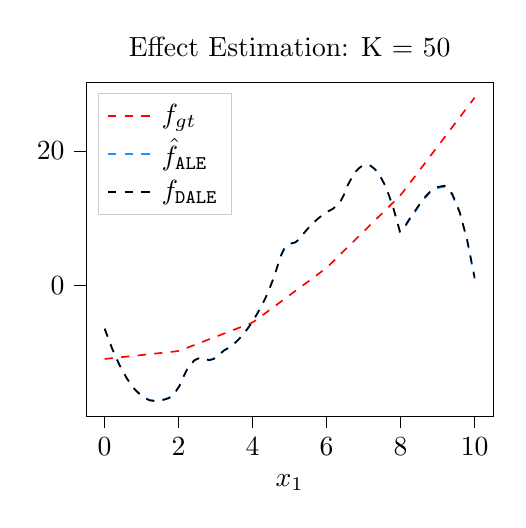
\begin{tikzpicture}

\definecolor{darkgray176}{RGB}{176,176,176}
\definecolor{dodgerblue}{RGB}{30,144,255}
\definecolor{lightgray204}{RGB}{204,204,204}

\begin{axis}[
legend cell align={left},
legend style={
  fill opacity=0.8,
  draw opacity=1,
  text opacity=1,
  at={(0.03,0.97)},
  anchor=north west,
  draw=lightgray204
},
tick align=outside,
tick pos=left,
title={Effect Estimation: K = 50},
x grid style={darkgray176},
xlabel={\(\displaystyle x_1\)},
xmin=-0.5, xmax=10.5,
xtick style={color=black},
y grid style={darkgray176},
ymin=-19.4760430884528, ymax=30.198088264309,
ytick style={color=black}
]
\addplot [semithick, red, dashed]
table {%
0 -10.9310787275426
0.101010101010101 -10.8718519947647
0.202020202020202 -10.8126252619868
0.303030303030303 -10.7533985292089
0.404040404040404 -10.6941717964309
0.505050505050505 -10.634945063653
0.606060606060606 -10.5757183308751
0.707070707070707 -10.5164915980972
0.808080808080808 -10.4572648653193
0.909090909090909 -10.3980381325414
1.01010101010101 -10.3388113997635
1.11111111111111 -10.2795846669856
1.21212121212121 -10.2203579342076
1.31313131313131 -10.1611312014297
1.41414141414141 -10.1019044686518
1.51515151515152 -10.0426777358739
1.61616161616162 -9.983451003096
1.71717171717172 -9.92422427031809
1.81818181818182 -9.86499753754018
1.91919191919192 -9.80577080476226
2.02020202020202 -9.71551411153251
2.12121212121212 -9.50113757649542
2.22222222222222 -9.28676104145832
2.32323232323232 -9.07238450642122
2.42424242424242 -8.85800797138412
2.52525252525253 -8.64363143634702
2.62626262626263 -8.42925490130992
2.72727272727273 -8.21487836627283
2.82828282828283 -8.00050183123573
2.92929292929293 -7.78612529619863
3.03030303030303 -7.57174876116153
3.13131313131313 -7.35737222612443
3.23232323232323 -7.14299569108734
3.33333333333333 -6.92861915605024
3.43434343434343 -6.71424262101314
3.53535353535354 -6.49986608597604
3.63636363636364 -6.28548955093894
3.73737373737374 -6.07111301590184
3.83838383838384 -5.85673648086475
3.93939393939394 -5.64235994582765
4.04040404040404 -5.34929709544007
4.14141414141414 -4.93820477202678
4.24242424242424 -4.52711244861348
4.34343434343434 -4.11602012520019
4.44444444444444 -3.70492780178689
4.54545454545454 -3.2938354783736
4.64646464646465 -2.8827431549603
4.74747474747475 -2.47165083154701
4.84848484848485 -2.06055850813371
4.94949494949495 -1.64946618472042
5.05050505050505 -1.23837386130712
5.15151515151515 -0.827281537893828
5.25252525252525 -0.416189214480532
5.35353535353535 -0.00509689106723599
5.45454545454545 0.405995432346057
5.55555555555556 0.817087755759353
5.65656565656566 1.22818007917265
5.75757575757576 1.63927240258595
5.85858585858586 2.05036472599924
5.95959595959596 2.46145704941253
6.06060606060606 2.95336271541685
6.16161616161616 3.49914394314852
6.26262626262626 4.04492517088019
6.36363636363636 4.59070639861185
6.46464646464646 5.13648762634352
6.56565656565657 5.68226885407519
6.66666666666667 6.22805008180686
6.76767676767677 6.77383130953853
6.86868686868687 7.3196125372702
6.96969696969697 7.86539376500187
7.07070707070707 8.41117499273354
7.17171717171717 8.9569562204652
7.27272727272727 9.50273744819687
7.37373737373737 10.0485186759285
7.47474747474747 10.5942999036602
7.57575757575758 11.1400811313919
7.67676767676768 11.6858623591235
7.77777777777778 12.2316435868552
7.87878787878788 12.7774248145869
7.97979797979798 13.3232060423185
8.08080808080808 14.0185364662469
8.18181818181818 14.7512541892244
8.28282828282828 15.4839719122019
8.38383838383838 16.2166896351795
8.48484848484848 16.949407358157
8.58585858585859 17.6821250811345
8.68686868686869 18.414842804112
8.78787878787879 19.1475605270896
8.88888888888889 19.8802782500671
8.98989898989899 20.6129959730446
9.09090909090909 21.3457136960221
9.19191919191919 22.0784314189997
9.29292929292929 22.8111491419772
9.39393939393939 23.5438668649547
9.49494949494949 24.2765845879322
9.5959595959596 25.0093023109097
9.6969696969697 25.7420200338873
9.7979797979798 26.4747377568648
9.8989898989899 27.2074554798423
10 27.9401732028198
};
\addlegendentry{$f_{gt}$}
\addplot [semithick, dodgerblue, dashed]
table {%
0 -6.39155669428798
0.101010101010101 -7.87176280822547
0.202020202020202 -9.34727774193452
0.303030303030303 -10.5929248444498
0.404040404040404 -11.8291895865083
0.505050505050505 -12.8402776776014
0.606060606060606 -13.8372922280092
0.707070707070707 -14.6138213076802
0.808080808080808 -15.3715856664374
0.909090909090909 -15.9135557346862
1.01010101010101 -16.4320699017928
1.11111111111111 -16.7394809586194
1.21212121212121 -17.0187449340754
1.31313131313131 -17.0915969794799
1.41414141414141 -17.1390709867376
1.51515151515152 -17.0306513310941
1.61616161616162 -16.9109325059248
1.71717171717172 -16.7318930407455
1.81818181818182 -16.4555098305769
1.91919191919192 -15.7356717821235
2.02020202020202 -14.9076740170153
2.12121212121212 -13.6470373852877
2.22222222222222 -12.4962403759351
2.32323232323232 -11.7348747550031
2.42424242424242 -11.093334176662
2.52525252525253 -10.8312395665255
2.62626262626263 -10.6989554191958
2.72727272727273 -10.9361318198549
2.82828282828283 -11.0627294254506
2.92929292929293 -10.9049815580264
3.03030303030303 -10.6345662571234
3.13131313131313 -10.1012602781034
3.23232323232323 -9.63635107348708
3.33333333333333 -9.31678501447877
3.43434343434343 -8.94376024612085
3.53535353535354 -8.46696268902541
3.63636363636364 -7.93356179261861
3.73737373737374 -7.29953273743605
3.83838383838384 -6.60575571298038
3.93939393939394 -5.81449515971068
4.04040404040404 -4.96034200720614
4.14141414141414 -4.01184995584932
4.24242424242424 -2.99732067529591
4.34343434343434 -1.89159712585195
4.44444444444444 -0.632456814122395
4.54545454545454 0.821941195061565
4.64646464646465 2.43672945572594
4.74747474747475 4.23980192464994
4.84848484848485 5.42690167554034
4.94949494949495 5.94669764856101
5.05050505050505 6.27649174108182
5.15151515151515 6.41628395310279
5.25252525252525 6.85742169129592
5.35353535353535 7.57672453057107
5.45454545454545 8.23871800219692
5.55555555555556 8.85189238286224
5.65656565656566 9.40563482670607
5.75757575757576 9.91268074876157
5.85858585858586 10.3581721648234
5.95959595959596 10.759089628269
6.06060606060606 11.0963300165488
6.16161616161616 11.3911190213847
6.26262626262626 11.8393282971996
6.36363636363636 12.3815693520016
6.46464646464646 13.4679123153837
6.56565656565657 14.8603126023421
6.66666666666667 15.932812724597
6.76767676767677 16.8405157923076
6.86868686868687 17.4186247509298
6.96969696969697 17.8416305993927
7.07070707070707 17.9253483943822
7.17171717171717 17.8636570235973
7.27272727272727 17.4443427206789
7.37373737373737 16.8859528330418
7.47474747474747 15.9600060429342
7.57575757575758 14.904917638445
7.67676767676768 13.4723383611482
7.77777777777778 11.9205514398069
7.87878787878788 9.98133967532086
7.97979797979798 7.93285423712737
8.08080808080808 8.30266103676541
8.18181818181818 9.27704089586134
8.28282828282828 10.104277296101
8.38383838383838 10.8992139126892
8.48484848484848 11.7249774233963
8.58585858585859 12.5566127234592
8.68686868686869 13.1768443933903
8.78787878787879 13.7626615188813
8.88888888888889 14.1321586507491
8.98989898989899 14.4721576016682
9.09090909090909 14.5909201954726
9.19191919191919 14.6851009718198
9.29292929292929 14.1088782566094
9.39393939393939 13.4743595856113
9.49494949494949 12.1548634341086
9.5959595959596 10.7916453157653
9.6969696969697 8.72887572797042
9.7979797979798 6.63695816228179
9.8989898989899 3.83091513819474
10 1.01029812516082
};
\addlegendentry{$\hat{f}_{\mathtt{ALE}}$}
\addplot [semithick, black, dashed]
table {%
0 -6.45366251536115
0.101010101010101 -7.93386862929863
0.202020202020202 -9.40939215334604
0.303030303030303 -10.6554687727793
0.404040404040404 -11.8921802124325
0.505050505050505 -12.9041273373615
0.606060606060606 -13.9020266926204
0.707070707070707 -14.6798443230453
0.808080808080808 -15.4389315939098
0.909090909090909 -15.9826197298305
1.01010101010101 -16.5028949163008
1.11111111111111 -16.8124535577173
1.21212121212121 -17.0939166597933
1.31313131313131 -17.1693458067056
1.41414141414141 -17.2181280269636
1.51515151515152 -17.1032219834882
1.61616161616162 -16.9773499822643
1.71717171717172 -16.7939067028611
1.81818181818182 -16.513516021749
1.91919191919192 -15.7914760661846
2.02020202020202 -14.961716775388
2.12121212121212 -13.7010801436624
2.22222222222222 -12.5502831343115
2.32323232323232 -11.7889175133799
2.42424242424242 -11.1473769350387
2.52525252525253 -10.885282324901
2.62626262626263 -10.7529981775697
2.72727272727273 -10.9901745782258
2.82828282828283 -11.1193372632691
2.92929292929293 -10.9707503938794
3.03030303030303 -10.6974283363254
3.13131313131313 -10.1330575063879
3.23232323232323 -9.64702420314582
3.33333333333333 -9.32745814413132
3.43434343434343 -8.9544333757688
3.53535353535354 -8.47763581867191
3.63636363636364 -7.94423492226536
3.73737373737374 -7.31020586708608
3.83838383838384 -6.61642884263549
3.93939393939394 -5.82516828937382
4.04040404040404 -4.9710151368792
4.14141414141414 -4.02252308553515
4.24242424242424 -3.00799380499648
4.34343434343434 -1.90227025557004
4.44444444444444 -0.643129943869416
4.54545454545454 0.811268065271056
4.64646464646465 2.42605632588
4.74747474747475 4.22912879473452
4.84848484848485 5.4163414868529
4.94949494949495 5.93637275417377
5.05050505050505 6.26617864414722
5.15151515151515 6.40575915677326
5.25252525252525 6.84679527925021
5.35353535353535 7.56609811851261
5.45454545454545 8.22809159012897
5.55555555555556 8.84126597078759
5.65656565656566 9.39500841462811
5.75757575757576 9.90205433668296
5.85858585858586 10.3475457527476
5.95959595959596 10.7484632161987
6.06060606060606 11.0857036044875
6.16161616161616 11.3804926093348
6.26262626262626 11.8288958481355
6.36363636363636 12.3714497464561
6.46464646464646 13.4606099564982
6.56565656565657 14.8572362168836
6.66666666666667 15.9330325984142
6.76767676767677 16.8435529817469
6.86868686868687 17.4235213686838
6.96969696969697 17.8479358749637
7.07070707070707 17.9320762673068
7.17171717171717 17.870384896534
7.27272727272727 17.4554824855752
7.37373737373737 16.9032202256552
7.47474747474747 15.9879355077662
7.57575757575758 14.945102358699
7.67676767676768 13.5294353338799
7.77777777777778 11.9960312956654
7.87878787878788 10.0799819639161
7.97979797979798 8.05600703655439
8.08080808080808 8.43976704288982
8.18181818181818 9.42546078264953
8.28282828282828 10.2583595903086
8.38383838383838 11.0577180470188
8.48484848484848 11.8841890521459
8.58585858585859 12.7158243522095
8.68686868686869 13.3360560221302
8.78787878787879 13.9218731476089
8.88888888888889 14.291370279453
8.98989898989899 14.6313692303469
9.09090909090909 14.7501318241145
9.19191919191919 14.8443126004235
9.29292929292929 14.2680899176152
9.39393939393939 13.6335712818401
9.49494949494949 12.3140751987059
9.5959595959596 10.9508571508466
9.6969696969697 8.88808766738661
9.7979797979798 6.79617020744323
9.8989898989899 3.99012732365734
10 1.16951045162982
};
\addlegendentry{$f_{\mathtt{DALE}}$}
\end{axis}

\end{tikzpicture}
}
    \resizebox{.32\columnwidth}{!}{% This file was created with tikzplotlib v0.10.1.
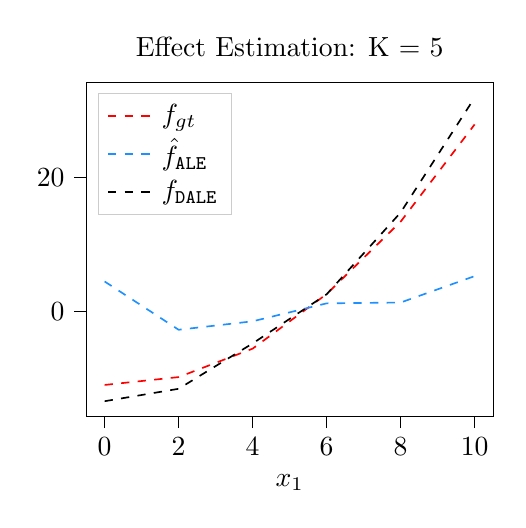
\begin{tikzpicture}

\definecolor{darkgray176}{RGB}{176,176,176}
\definecolor{dodgerblue}{RGB}{30,144,255}
\definecolor{lightgray204}{RGB}{204,204,204}

\begin{axis}[
legend cell align={left},
legend style={
  fill opacity=0.8,
  draw opacity=1,
  text opacity=1,
  at={(0.03,0.97)},
  anchor=north west,
  draw=lightgray204
},
tick align=outside,
tick pos=left,
title={Effect Estimation: K = 5},
x grid style={darkgray176},
xlabel={\(\displaystyle x_1\)},
xmin=-0.5, xmax=10.5,
xtick style={color=black},
y grid style={darkgray176},
ymin=-15.623228566917, ymax=34.2007169448902,
ytick style={color=black}
]
\addplot [semithick, red, dashed]
table {%
0 -10.9310787275426
0.01001001001001 -10.9252094116817
0.02002002002002 -10.9193400958208
0.03003003003003 -10.91347077996
0.04004004004004 -10.9076014640991
0.05005005005005 -10.9017321482382
0.0600600600600601 -10.8958628323774
0.0700700700700701 -10.8899935165165
0.0800800800800801 -10.8841242006556
0.0900900900900901 -10.8782548847947
0.1001001001001 -10.8723855689339
0.11011011011011 -10.866516253073
0.12012012012012 -10.8606469372121
0.13013013013013 -10.8547776213512
0.14014014014014 -10.8489083054904
0.15015015015015 -10.8430389896295
0.16016016016016 -10.8371696737686
0.17017017017017 -10.8313003579077
0.18018018018018 -10.8254310420469
0.19019019019019 -10.819561726186
0.2002002002002 -10.8136924103251
0.21021021021021 -10.8078230944642
0.22022022022022 -10.8019537786034
0.23023023023023 -10.7960844627425
0.24024024024024 -10.7902151468816
0.25025025025025 -10.7843458310207
0.26026026026026 -10.7784765151599
0.27027027027027 -10.772607199299
0.28028028028028 -10.7667378834381
0.29029029029029 -10.7608685675772
0.3003003003003 -10.7549992517164
0.31031031031031 -10.7491299358555
0.32032032032032 -10.7432606199946
0.33033033033033 -10.7373913041337
0.34034034034034 -10.7315219882729
0.35035035035035 -10.725652672412
0.36036036036036 -10.7197833565511
0.37037037037037 -10.7139140406903
0.38038038038038 -10.7080447248294
0.39039039039039 -10.7021754089685
0.4004004004004 -10.6963060931076
0.41041041041041 -10.6904367772468
0.42042042042042 -10.6845674613859
0.43043043043043 -10.678698145525
0.44044044044044 -10.6728288296641
0.45045045045045 -10.6669595138033
0.46046046046046 -10.6610901979424
0.47047047047047 -10.6552208820815
0.48048048048048 -10.6493515662206
0.49049049049049 -10.6434822503598
0.500500500500501 -10.6376129344989
0.510510510510511 -10.631743618638
0.520520520520521 -10.6258743027771
0.530530530530531 -10.6200049869163
0.540540540540541 -10.6141356710554
0.550550550550551 -10.6082663551945
0.560560560560561 -10.6023970393336
0.570570570570571 -10.5965277234728
0.580580580580581 -10.5906584076119
0.590590590590591 -10.584789091751
0.600600600600601 -10.5789197758901
0.610610610610611 -10.5730504600293
0.620620620620621 -10.5671811441684
0.630630630630631 -10.5613118283075
0.640640640640641 -10.5554425124466
0.650650650650651 -10.5495731965858
0.660660660660661 -10.5437038807249
0.670670670670671 -10.537834564864
0.680680680680681 -10.5319652490032
0.690690690690691 -10.5260959331423
0.700700700700701 -10.5202266172814
0.710710710710711 -10.5143573014205
0.720720720720721 -10.5084879855597
0.730730730730731 -10.5026186696988
0.740740740740741 -10.4967493538379
0.750750750750751 -10.490880037977
0.760760760760761 -10.4850107221162
0.770770770770771 -10.4791414062553
0.780780780780781 -10.4732720903944
0.790790790790791 -10.4674027745335
0.800800800800801 -10.4615334586727
0.810810810810811 -10.4556641428118
0.820820820820821 -10.4497948269509
0.830830830830831 -10.44392551109
0.840840840840841 -10.4380561952292
0.850850850850851 -10.4321868793683
0.860860860860861 -10.4263175635074
0.870870870870871 -10.4204482476465
0.880880880880881 -10.4145789317857
0.890890890890891 -10.4087096159248
0.900900900900901 -10.4028403000639
0.910910910910911 -10.396970984203
0.920920920920921 -10.3911016683422
0.930930930930931 -10.3852323524813
0.940940940940941 -10.3793630366204
0.950950950950951 -10.3734937207595
0.960960960960961 -10.3676244048987
0.970970970970971 -10.3617550890378
0.980980980980981 -10.3558857731769
0.990990990990991 -10.3500164573161
1.001001001001 -10.3441471414552
1.01101101101101 -10.3382778255943
1.02102102102102 -10.3324085097334
1.03103103103103 -10.3265391938726
1.04104104104104 -10.3206698780117
1.05105105105105 -10.3148005621508
1.06106106106106 -10.3089312462899
1.07107107107107 -10.3030619304291
1.08108108108108 -10.2971926145682
1.09109109109109 -10.2913232987073
1.1011011011011 -10.2854539828464
1.11111111111111 -10.2795846669856
1.12112112112112 -10.2737153511247
1.13113113113113 -10.2678460352638
1.14114114114114 -10.2619767194029
1.15115115115115 -10.2561074035421
1.16116116116116 -10.2502380876812
1.17117117117117 -10.2443687718203
1.18118118118118 -10.2384994559594
1.19119119119119 -10.2326301400986
1.2012012012012 -10.2267608242377
1.21121121121121 -10.2208915083768
1.22122122122122 -10.2150221925159
1.23123123123123 -10.2091528766551
1.24124124124124 -10.2032835607942
1.25125125125125 -10.1974142449333
1.26126126126126 -10.1915449290724
1.27127127127127 -10.1856756132116
1.28128128128128 -10.1798062973507
1.29129129129129 -10.1739369814898
1.3013013013013 -10.168067665629
1.31131131131131 -10.1621983497681
1.32132132132132 -10.1563290339072
1.33133133133133 -10.1504597180463
1.34134134134134 -10.1445904021855
1.35135135135135 -10.1387210863246
1.36136136136136 -10.1328517704637
1.37137137137137 -10.1269824546028
1.38138138138138 -10.121113138742
1.39139139139139 -10.1152438228811
1.4014014014014 -10.1093745070202
1.41141141141141 -10.1035051911593
1.42142142142142 -10.0976358752985
1.43143143143143 -10.0917665594376
1.44144144144144 -10.0858972435767
1.45145145145145 -10.0800279277158
1.46146146146146 -10.074158611855
1.47147147147147 -10.0682892959941
1.48148148148148 -10.0624199801332
1.49149149149149 -10.0565506642723
1.5015015015015 -10.0506813484115
1.51151151151151 -10.0448120325506
1.52152152152152 -10.0389427166897
1.53153153153153 -10.0330734008288
1.54154154154154 -10.027204084968
1.55155155155155 -10.0213347691071
1.56156156156156 -10.0154654532462
1.57157157157157 -10.0095961373853
1.58158158158158 -10.0037268215245
1.59159159159159 -9.9978575056636
1.6016016016016 -9.99198818980273
1.61161161161161 -9.98611887394185
1.62162162162162 -9.98024955808098
1.63163163163163 -9.9743802422201
1.64164164164164 -9.96851092635923
1.65165165165165 -9.96264161049836
1.66166166166166 -9.95677229463748
1.67167167167167 -9.95090297877661
1.68168168168168 -9.94503366291573
1.69169169169169 -9.93916434705486
1.7017017017017 -9.93329503119399
1.71171171171171 -9.92742571533311
1.72172172172172 -9.92155639947224
1.73173173173173 -9.91568708361136
1.74174174174174 -9.90981776775049
1.75175175175175 -9.90394845188961
1.76176176176176 -9.89807913602874
1.77177177177177 -9.89220982016787
1.78178178178178 -9.88634050430699
1.79179179179179 -9.88047118844612
1.8018018018018 -9.87460187258524
1.81181181181181 -9.86873255672437
1.82182182182182 -9.86286324086349
1.83183183183183 -9.85699392500262
1.84184184184184 -9.85112460914175
1.85185185185185 -9.84525529328087
1.86186186186186 -9.83938597742
1.87187187187187 -9.83351666155912
1.88188188188188 -9.82764734569825
1.89189189189189 -9.82177802983738
1.9019019019019 -9.8159087139765
1.91191191191191 -9.81003939811563
1.92192192192192 -9.80417008225475
1.93193193193193 -9.79830076639388
1.94194194194194 -9.792431450533
1.95195195195195 -9.78656213467213
1.96196196196196 -9.78069281881126
1.97197197197197 -9.77482350295038
1.98198198198198 -9.76895418708951
1.99199199199199 -9.76308487122863
2.002002002002 -9.7541405142419
2.01201201201201 -9.73289599275174
2.02202202202202 -9.71165147126158
2.03203203203203 -9.69040694977141
2.04204204204204 -9.66916242828125
2.05205205205205 -9.64791790679109
2.06206206206206 -9.62667338530092
2.07207207207207 -9.60542886381076
2.08208208208208 -9.5841843423206
2.09209209209209 -9.56293982083043
2.1021021021021 -9.54169529934027
2.11211211211211 -9.52045077785011
2.12212212212212 -9.49920625635995
2.13213213213213 -9.47796173486978
2.14214214214214 -9.45671721337962
2.15215215215215 -9.43547269188946
2.16216216216216 -9.41422817039929
2.17217217217217 -9.39298364890913
2.18218218218218 -9.37173912741897
2.19219219219219 -9.35049460592881
2.2022022022022 -9.32925008443864
2.21221221221221 -9.30800556294848
2.22222222222222 -9.28676104145832
2.23223223223223 -9.26551651996815
2.24224224224224 -9.24427199847799
2.25225225225225 -9.22302747698783
2.26226226226226 -9.20178295549767
2.27227227227227 -9.1805384340075
2.28228228228228 -9.15929391251734
2.29229229229229 -9.13804939102718
2.3023023023023 -9.11680486953701
2.31231231231231 -9.09556034804685
2.32232232232232 -9.07431582655669
2.33233233233233 -9.05307130506653
2.34234234234234 -9.03182678357636
2.35235235235235 -9.0105822620862
2.36236236236236 -8.98933774059604
2.37237237237237 -8.96809321910587
2.38238238238238 -8.94684869761571
2.39239239239239 -8.92560417612555
2.4024024024024 -8.90435965463539
2.41241241241241 -8.88311513314522
2.42242242242242 -8.86187061165506
2.43243243243243 -8.8406260901649
2.44244244244244 -8.81938156867473
2.45245245245245 -8.79813704718457
2.46246246246246 -8.77689252569441
2.47247247247247 -8.75564800420425
2.48248248248248 -8.73440348271408
2.49249249249249 -8.71315896122392
2.5025025025025 -8.69191443973376
2.51251251251251 -8.67066991824359
2.52252252252252 -8.64942539675343
2.53253253253253 -8.62818087526327
2.54254254254254 -8.6069363537731
2.55255255255255 -8.58569183228294
2.56256256256256 -8.56444731079278
2.57257257257257 -8.54320278930262
2.58258258258258 -8.52195826781245
2.59259259259259 -8.50071374632229
2.6026026026026 -8.47946922483213
2.61261261261261 -8.45822470334197
2.62262262262262 -8.4369801818518
2.63263263263263 -8.41573566036164
2.64264264264264 -8.39449113887148
2.65265265265265 -8.37324661738131
2.66266266266266 -8.35200209589115
2.67267267267267 -8.33075757440099
2.68268268268268 -8.30951305291082
2.69269269269269 -8.28826853142066
2.7027027027027 -8.2670240099305
2.71271271271271 -8.24577948844034
2.72272272272272 -8.22453496695017
2.73273273273273 -8.20329044546001
2.74274274274274 -8.18204592396985
2.75275275275275 -8.16080140247968
2.76276276276276 -8.13955688098952
2.77277277277277 -8.11831235949936
2.78278278278278 -8.0970678380092
2.79279279279279 -8.07582331651903
2.8028028028028 -8.05457879502887
2.81281281281281 -8.03333427353871
2.82282282282282 -8.01208975204855
2.83283283283283 -7.99084523055838
2.84284284284284 -7.96960070906822
2.85285285285285 -7.94835618757806
2.86286286286286 -7.92711166608789
2.87287287287287 -7.90586714459773
2.88288288288288 -7.88462262310757
2.89289289289289 -7.8633781016174
2.9029029029029 -7.84213358012724
2.91291291291291 -7.82088905863708
2.92292292292292 -7.79964453714692
2.93293293293293 -7.77840001565675
2.94294294294294 -7.75715549416659
2.95295295295295 -7.73591097267643
2.96296296296296 -7.71466645118626
2.97297297297297 -7.6934219296961
2.98298298298298 -7.67217740820594
2.99299299299299 -7.65093288671578
3.003003003003 -7.62968836522561
3.01301301301301 -7.60844384373545
3.02302302302302 -7.58719932224529
3.03303303303303 -7.56595480075512
3.04304304304304 -7.54471027926496
3.05305305305305 -7.5234657577748
3.06306306306306 -7.50222123628463
3.07307307307307 -7.48097671479447
3.08308308308308 -7.45973219330431
3.09309309309309 -7.43848767181415
3.1031031031031 -7.41724315032398
3.11311311311311 -7.39599862883382
3.12312312312312 -7.37475410734366
3.13313313313313 -7.3535095858535
3.14314314314314 -7.33226506436333
3.15315315315315 -7.31102054287317
3.16316316316316 -7.28977602138301
3.17317317317317 -7.26853149989284
3.18318318318318 -7.24728697840268
3.19319319319319 -7.22604245691252
3.2032032032032 -7.20479793542236
3.21321321321321 -7.18355341393219
3.22322322322322 -7.16230889244203
3.23323323323323 -7.14106437095187
3.24324324324324 -7.1198198494617
3.25325325325325 -7.09857532797154
3.26326326326326 -7.07733080648138
3.27327327327327 -7.05608628499121
3.28328328328328 -7.03484176350105
3.29329329329329 -7.01359724201089
3.3033033033033 -6.99235272052073
3.31331331331331 -6.97110819903056
3.32332332332332 -6.9498636775404
3.33333333333333 -6.92861915605024
3.34334334334334 -6.90737463456007
3.35335335335335 -6.88613011306991
3.36336336336336 -6.86488559157975
3.37337337337337 -6.84364107008959
3.38338338338338 -6.82239654859942
3.39339339339339 -6.80115202710926
3.4034034034034 -6.7799075056191
3.41341341341341 -6.75866298412893
3.42342342342342 -6.73741846263877
3.43343343343343 -6.71617394114861
3.44344344344344 -6.69492941965845
3.45345345345345 -6.67368489816828
3.46346346346346 -6.65244037667812
3.47347347347347 -6.63119585518796
3.48348348348348 -6.60995133369779
3.49349349349349 -6.58870681220763
3.5035035035035 -6.56746229071747
3.51351351351351 -6.54621776922731
3.52352352352352 -6.52497324773714
3.53353353353353 -6.50372872624698
3.54354354354354 -6.48248420475682
3.55355355355355 -6.46123968326665
3.56356356356356 -6.43999516177649
3.57357357357357 -6.41875064028633
3.58358358358358 -6.39750611879617
3.59359359359359 -6.376261597306
3.6036036036036 -6.35501707581584
3.61361361361361 -6.33377255432568
3.62362362362362 -6.31252803283551
3.63363363363363 -6.29128351134535
3.64364364364364 -6.27003898985519
3.65365365365365 -6.24879446836503
3.66366366366366 -6.22754994687486
3.67367367367367 -6.2063054253847
3.68368368368368 -6.18506090389454
3.69369369369369 -6.16381638240437
3.7037037037037 -6.14257186091421
3.71371371371371 -6.12132733942405
3.72372372372372 -6.10008281793388
3.73373373373373 -6.07883829644372
3.74374374374374 -6.05759377495356
3.75375375375375 -6.0363492534634
3.76376376376376 -6.01510473197323
3.77377377377377 -5.99386021048307
3.78378378378378 -5.97261568899291
3.79379379379379 -5.95137116750274
3.8038038038038 -5.93012664601258
3.81381381381381 -5.90888212452242
3.82382382382382 -5.88763760303226
3.83383383383383 -5.86639308154209
3.84384384384384 -5.84514856005193
3.85385385385385 -5.82390403856177
3.86386386386386 -5.8026595170716
3.87387387387387 -5.78141499558144
3.88388388388388 -5.76017047409128
3.89389389389389 -5.73892595260112
3.9039039039039 -5.71768143111095
3.91391391391391 -5.69643690962079
3.92392392392392 -5.67519238813063
3.93393393393393 -5.65394786664046
3.94394394394394 -5.6327033451503
3.95395395395395 -5.61145882366014
3.96396396396396 -5.59021430216998
3.97397397397397 -5.56896978067981
3.98398398398398 -5.54772525918965
3.99399399399399 -5.52648073769949
4.004004004004 -5.49743847324666
4.01401401401401 -5.45669959434985
4.02402402402402 -5.41596071545304
4.03403403403403 -5.37522183655622
4.04404404404404 -5.33448295765941
4.05405405405405 -5.2937440787626
4.06406406406406 -5.25300519986578
4.07407407407407 -5.21226632096897
4.08408408408408 -5.17152744207216
4.09409409409409 -5.13078856317535
4.1041041041041 -5.09004968427853
4.11411411411411 -5.04931080538172
4.12412412412412 -5.00857192648491
4.13413413413413 -4.96783304758809
4.14414414414414 -4.92709416869128
4.15415415415415 -4.88635528979447
4.16416416416416 -4.84561641089765
4.17417417417417 -4.80487753200084
4.18418418418418 -4.76413865310403
4.19419419419419 -4.72339977420722
4.2042042042042 -4.6826608953104
4.21421421421421 -4.64192201641359
4.22422422422422 -4.60118313751678
4.23423423423423 -4.56044425861996
4.24424424424424 -4.51970537972315
4.25425425425425 -4.47896650082634
4.26426426426426 -4.43822762192952
4.27427427427427 -4.39748874303271
4.28428428428428 -4.3567498641359
4.29429429429429 -4.31601098523909
4.3043043043043 -4.27527210634227
4.31431431431431 -4.23453322744546
4.32432432432432 -4.19379434854865
4.33433433433433 -4.15305546965183
4.34434434434434 -4.11231659075502
4.35435435435435 -4.07157771185821
4.36436436436436 -4.03083883296139
4.37437437437437 -3.99009995406458
4.38438438438438 -3.94936107516777
4.39439439439439 -3.90862219627096
4.4044044044044 -3.86788331737414
4.41441441441441 -3.82714443847733
4.42442442442442 -3.78640555958052
4.43443443443443 -3.7456666806837
4.44444444444444 -3.70492780178689
4.45445445445445 -3.66418892289008
4.46446446446446 -3.62345004399326
4.47447447447447 -3.58271116509645
4.48448448448448 -3.54197228619964
4.49449449449449 -3.50123340730283
4.5045045045045 -3.46049452840601
4.51451451451451 -3.4197556495092
4.52452452452452 -3.37901677061239
4.53453453453453 -3.33827789171557
4.54454454454454 -3.29753901281876
4.55455455455455 -3.25680013392195
4.56456456456456 -3.21606125502514
4.57457457457457 -3.17532237612832
4.58458458458458 -3.13458349723151
4.59459459459459 -3.0938446183347
4.6046046046046 -3.05310573943788
4.61461461461461 -3.01236686054107
4.62462462462462 -2.97162798164426
4.63463463463463 -2.93088910274744
4.64464464464464 -2.89015022385063
4.65465465465465 -2.84941134495382
4.66466466466466 -2.808672466057
4.67467467467467 -2.76793358716019
4.68468468468468 -2.72719470826338
4.69469469469469 -2.68645582936657
4.7047047047047 -2.64571695046975
4.71471471471471 -2.60497807157294
4.72472472472472 -2.56423919267613
4.73473473473473 -2.52350031377931
4.74474474474474 -2.4827614348825
4.75475475475475 -2.44202255598569
4.76476476476476 -2.40128367708888
4.77477477477477 -2.36054479819206
4.78478478478478 -2.31980591929525
4.79479479479479 -2.27906704039844
4.8048048048048 -2.23832816150162
4.81481481481481 -2.19758928260481
4.82482482482482 -2.156850403708
4.83483483483483 -2.11611152481118
4.84484484484484 -2.07537264591437
4.85485485485485 -2.03463376701756
4.86486486486486 -1.99389488812074
4.87487487487487 -1.95315600922393
4.88488488488488 -1.91241713032712
4.89489489489489 -1.87167825143031
4.9049049049049 -1.83093937253349
4.91491491491491 -1.79020049363668
4.92492492492492 -1.74946161473987
4.93493493493493 -1.70872273584305
4.94494494494494 -1.66798385694624
4.95495495495495 -1.62724497804943
4.96496496496496 -1.58650609915261
4.97497497497497 -1.5457672202558
4.98498498498498 -1.50502834135899
4.99499499499499 -1.46428946246218
5.00500500500501 -1.42355058356536
5.01501501501502 -1.38281170466855
5.02502502502503 -1.34207282577174
5.03503503503504 -1.30133394687492
5.04504504504505 -1.26059506797811
5.05505505505506 -1.2198561890813
5.06506506506507 -1.17911731018448
5.07507507507508 -1.13837843128767
5.08508508508509 -1.09763955239086
5.0950950950951 -1.05690067349405
5.10510510510511 -1.01616179459723
5.11511511511512 -0.97542291570042
5.12512512512513 -0.934684036803606
5.13513513513514 -0.893945157906794
5.14514514514515 -0.853206279009981
5.15515515515516 -0.812467400113167
5.16516516516517 -0.771728521216353
5.17517517517518 -0.730989642319543
5.18518518518519 -0.690250763422728
5.1951951951952 -0.649511884525914
5.20520520520521 -0.608773005629104
5.21521521521522 -0.568034126732289
5.22522522522523 -0.527295247835475
5.23523523523524 -0.486556368938665
5.24524524524525 -0.445817490041851
5.25525525525526 -0.405078611145036
5.26526526526527 -0.364339732248224
5.27527527527528 -0.323600853351412
5.28528528528529 -0.282861974454597
5.2952952952953 -0.242123095557785
5.30530530530531 -0.201384216660973
5.31531531531532 -0.160645337764159
5.32532532532533 -0.119906458867346
5.33533533533534 -0.0791675799705338
5.34534534534535 -0.0384287010737197
5.35535535535536 0.00231017782309273
5.36536536536537 0.0430490567199051
5.37537537537538 0.0837879356167193
5.38538538538539 0.124526814513532
5.3953953953954 0.165265693410344
5.40540540540541 0.206004572307158
5.41541541541542 0.246743451203971
5.42542542542543 0.287482330100783
5.43543543543544 0.328221208997597
5.44544544544545 0.368960087894409
5.45545545545546 0.409698966791222
5.46546546546547 0.450437845688036
5.47547547547548 0.491176724584848
5.48548548548549 0.531915603481661
5.4954954954955 0.572654482378475
5.50550550550551 0.613393361275287
5.51551551551552 0.6541322401721
5.52552552552553 0.694871119068914
5.53553553553554 0.735609997965726
5.54554554554555 0.776348876862539
5.55555555555556 0.817087755759353
5.56556556556557 0.857826634656165
5.57557557557558 0.898565513552978
5.58558558558559 0.939304392449792
5.5955955955956 0.980043271346606
5.60560560560561 1.02078215024342
5.61561561561562 1.06152102914023
5.62562562562563 1.10225990803704
5.63563563563564 1.14299878693386
5.64564564564565 1.18373766583067
5.65565565565566 1.22447654472748
5.66566566566567 1.26521542362429
5.67567567567568 1.30595430252111
5.68568568568569 1.34669318141792
5.6956956956957 1.38743206031473
5.70570570570571 1.42817093921155
5.71571571571572 1.46890981810836
5.72572572572573 1.50964869700517
5.73573573573574 1.55038757590199
5.74574574574575 1.5911264547988
5.75575575575576 1.63186533369561
5.76576576576577 1.67260421259243
5.77577577577578 1.71334309148924
5.78578578578579 1.75408197038605
5.7957957957958 1.79482084928286
5.80580580580581 1.83555972817968
5.81581581581582 1.87629860707649
5.82582582582583 1.9170374859733
5.83583583583584 1.95777636487012
5.84584584584585 1.99851524376693
5.85585585585586 2.03925412266374
5.86586586586587 2.07999300156056
5.87587587587588 2.12073188045737
5.88588588588589 2.16147075935418
5.8958958958959 2.202209638251
5.90590590590591 2.24294851714781
5.91591591591592 2.28368739604462
5.92592592592593 2.32442627494143
5.93593593593594 2.36516515383825
5.94594594594595 2.40590403273506
5.95595595595596 2.44664291163187
5.96596596596597 2.48738179052869
5.97597597597598 2.5281206694255
5.98598598598599 2.56885954832231
5.995995995996 2.60959842721912
6.00600600600601 2.65834583556189
6.01601601601602 2.7124322635353
6.02602602602603 2.76651869150871
6.03603603603604 2.82060511948212
6.04604604604605 2.87469154745553
6.05605605605606 2.92877797542894
6.06606606606607 2.98286440340235
6.07607607607608 3.03695083137575
6.08608608608609 3.09103725934916
6.0960960960961 3.14512368732257
6.10610610610611 3.19921011529598
6.11611611611612 3.25329654326939
6.12612612612613 3.3073829712428
6.13613613613614 3.3614693992162
6.14614614614615 3.41555582718961
6.15615615615616 3.46964225516302
6.16616616616617 3.52372868313643
6.17617617617618 3.57781511110984
6.18618618618619 3.63190153908325
6.1961961961962 3.68598796705666
6.20620620620621 3.74007439503007
6.21621621621622 3.79416082300347
6.22622622622623 3.84824725097688
6.23623623623624 3.90233367895029
6.24624624624625 3.9564201069237
6.25625625625626 4.01050653489711
6.26626626626627 4.06459296287052
6.27627627627628 4.11867939084392
6.28628628628629 4.17276581881733
6.2962962962963 4.22685224679074
6.30630630630631 4.28093867476415
6.31631631631632 4.33502510273756
6.32632632632633 4.38911153071097
6.33633633633634 4.44319795868438
6.34634634634635 4.49728438665778
6.35635635635636 4.55137081463119
6.36636636636637 4.6054572426046
6.37637637637638 4.65954367057801
6.38638638638639 4.71363009855142
6.3963963963964 4.76771652652483
6.40640640640641 4.82180295449824
6.41641641641642 4.87588938247165
6.42642642642643 4.92997581044506
6.43643643643644 4.98406223841847
6.44644644644645 5.03814866639187
6.45645645645646 5.09223509436528
6.46646646646647 5.14632152233869
6.47647647647648 5.2004079503121
6.48648648648649 5.25449437828551
6.4964964964965 5.30858080625892
6.50650650650651 5.36266723423233
6.51651651651652 5.41675366220574
6.52652652652653 5.47084009017914
6.53653653653654 5.52492651815255
6.54654654654655 5.57901294612596
6.55655655655656 5.63309937409937
6.56656656656657 5.68718580207278
6.57657657657658 5.74127223004619
6.58658658658659 5.79535865801959
6.5965965965966 5.849445085993
6.60660660660661 5.90353151396641
6.61661661661662 5.95761794193982
6.62662662662663 6.01170436991323
6.63663663663664 6.06579079788663
6.64664664664665 6.11987722586004
6.65665665665666 6.17396365383345
6.66666666666667 6.22805008180686
6.67667667667668 6.28213650978027
6.68668668668669 6.33622293775368
6.6966966966967 6.39030936572709
6.70670670670671 6.4443957937005
6.71671671671672 6.4984822216739
6.72672672672673 6.55256864964731
6.73673673673674 6.60665507762072
6.74674674674675 6.66074150559413
6.75675675675676 6.71482793356754
6.76676676676677 6.76891436154095
6.77677677677678 6.82300078951436
6.78678678678679 6.87708721748776
6.7967967967968 6.93117364546117
6.80680680680681 6.98526007343458
6.81681681681682 7.03934650140799
6.82682682682683 7.0934329293814
6.83683683683684 7.14751935735481
6.84684684684685 7.20160578532822
6.85685685685686 7.25569221330163
6.86686686686687 7.30977864127503
6.87687687687688 7.36386506924844
6.88688688688689 7.41795149722185
6.8968968968969 7.47203792519526
6.90690690690691 7.52612435316867
6.91691691691692 7.58021078114207
6.92692692692693 7.63429720911548
6.93693693693694 7.68838363708889
6.94694694694695 7.7424700650623
6.95695695695696 7.79655649303571
6.96696696696697 7.85064292100912
6.97697697697698 7.90472934898253
6.98698698698699 7.95881577695593
6.996996996997 8.01290220492934
7.00700700700701 8.06698863290275
7.01701701701702 8.12107506087616
7.02702702702703 8.17516148884957
7.03703703703704 8.22924791682298
7.04704704704705 8.28333434479639
7.05705705705706 8.33742077276979
7.06706706706707 8.3915072007432
7.07707707707708 8.44559362871661
7.08708708708709 8.49968005669002
7.0970970970971 8.55376648466343
7.10710710710711 8.60785291263684
7.11711711711712 8.66193934061025
7.12712712712713 8.71602576858366
7.13713713713714 8.77011219655706
7.14714714714715 8.82419862453047
7.15715715715716 8.87828505250388
7.16716716716717 8.93237148047729
7.17717717717718 8.9864579084507
7.18718718718719 9.04054433642411
7.1971971971972 9.09463076439751
7.20720720720721 9.14871719237092
7.21721721721722 9.20280362034433
7.22722722722723 9.25689004831774
7.23723723723724 9.31097647629115
7.24724724724725 9.36506290426455
7.25725725725726 9.41914933223796
7.26726726726727 9.47323576021137
7.27727727727728 9.52732218818478
7.28728728728729 9.58140861615819
7.2972972972973 9.6354950441316
7.30730730730731 9.68958147210501
7.31731731731732 9.74366790007841
7.32732732732733 9.79775432805182
7.33733733733734 9.85184075602523
7.34734734734735 9.90592718399864
7.35735735735736 9.96001361197205
7.36736736736737 10.0141000399455
7.37737737737738 10.0681864679189
7.38738738738739 10.1222728958923
7.3973973973974 10.1763593238657
7.40740740740741 10.2304457518391
7.41741741741742 10.2845321798125
7.42742742742743 10.3386186077859
7.43743743743744 10.3927050357593
7.44744744744745 10.4467914637327
7.45745745745746 10.5008778917061
7.46746746746747 10.5549643196795
7.47747747747748 10.609050747653
7.48748748748749 10.6631371756264
7.4974974974975 10.7172236035998
7.50750750750751 10.7713100315732
7.51751751751752 10.8253964595466
7.52752752752753 10.87948288752
7.53753753753754 10.9335693154934
7.54754754754755 10.9876557434668
7.55755755755756 11.0417421714402
7.56756756756757 11.0958285994136
7.57757757757758 11.149915027387
7.58758758758759 11.2040014553604
7.5975975975976 11.2580878833339
7.60760760760761 11.3121743113073
7.61761761761762 11.3662607392807
7.62762762762763 11.4203471672541
7.63763763763764 11.4744335952275
7.64764764764765 11.5285200232009
7.65765765765766 11.5826064511743
7.66766766766767 11.6366928791477
7.67767767767768 11.6907793071211
7.68768768768769 11.7448657350945
7.6976976976977 11.7989521630679
7.70770770770771 11.8530385910413
7.71771771771772 11.9071250190148
7.72772772772773 11.9612114469882
7.73773773773774 12.0152978749616
7.74774774774775 12.069384302935
7.75775775775776 12.1234707309084
7.76776776776777 12.1775571588818
7.77777777777778 12.2316435868552
7.78778778778779 12.2857300148286
7.7977977977978 12.339816442802
7.80780780780781 12.3939028707754
7.81781781781782 12.4479892987488
7.82782782782783 12.5020757267222
7.83783783783784 12.5561621546957
7.84784784784785 12.6102485826691
7.85785785785786 12.6643350106425
7.86786786786787 12.7184214386159
7.87787787787788 12.7725078665893
7.88788788788789 12.8265942945627
7.8978978978979 12.8806807225361
7.90790790790791 12.9347671505095
7.91791791791792 12.9888535784829
7.92792792792793 13.0429400064563
7.93793793793794 13.0970264344297
7.94794794794795 13.1511128624032
7.95795795795796 13.2051992903766
7.96796796796797 13.25928571835
7.97797797797798 13.3133721463234
7.98798798798799 13.3674585742968
7.997997997998 13.4215450022702
8.00800800800801 13.4904516208577
8.01801801801802 13.5630632870987
8.02802802802803 13.6356749533397
8.03803803803804 13.7082866195807
8.04804804804805 13.7808982858218
8.05805805805806 13.8535099520628
8.06806806806807 13.9261216183038
8.07807807807808 13.9987332845448
8.08808808808809 14.0713449507858
8.0980980980981 14.1439566170268
8.10810810810811 14.2165682832679
8.11811811811812 14.2891799495089
8.12812812812813 14.3617916157499
8.13813813813814 14.4344032819909
8.14814814814815 14.5070149482319
8.15815815815816 14.5796266144729
8.16816816816817 14.6522382807139
8.17817817817818 14.724849946955
8.18818818818819 14.797461613196
8.1981981981982 14.870073279437
8.20820820820821 14.942684945678
8.21821821821822 15.015296611919
8.22822822822823 15.08790827816
8.23823823823824 15.1605199444011
8.24824824824825 15.2331316106421
8.25825825825826 15.3057432768831
8.26826826826827 15.3783549431241
8.27827827827828 15.4509666093651
8.28828828828829 15.5235782756061
8.2982982982983 15.5961899418472
8.30830830830831 15.6688016080882
8.31831831831832 15.7414132743292
8.32832832832833 15.8140249405702
8.33833833833834 15.8866366068112
8.34834834834835 15.9592482730522
8.35835835835836 16.0318599392932
8.36836836836837 16.1044716055343
8.37837837837838 16.1770832717753
8.38838838838839 16.2496949380163
8.3983983983984 16.3223066042573
8.40840840840841 16.3949182704983
8.41841841841842 16.4675299367393
8.42842842842843 16.5401416029804
8.43843843843844 16.6127532692214
8.44844844844845 16.6853649354624
8.45845845845846 16.7579766017034
8.46846846846847 16.8305882679444
8.47847847847848 16.9031999341854
8.48848848848849 16.9758116004265
8.4984984984985 17.0484232666675
8.50850850850851 17.1210349329085
8.51851851851852 17.1936465991495
8.52852852852853 17.2662582653905
8.53853853853854 17.3388699316315
8.54854854854855 17.4114815978725
8.55855855855856 17.4840932641136
8.56856856856857 17.5567049303546
8.57857857857858 17.6293165965956
8.58858858858859 17.7019282628366
8.5985985985986 17.7745399290776
8.60860860860861 17.8471515953186
8.61861861861862 17.9197632615597
8.62862862862863 17.9923749278007
8.63863863863864 18.0649865940417
8.64864864864865 18.1375982602827
8.65865865865866 18.2102099265237
8.66866866866867 18.2828215927647
8.67867867867868 18.3554332590058
8.68868868868869 18.4280449252468
8.6986986986987 18.5006565914878
8.70870870870871 18.5732682577288
8.71871871871872 18.6458799239698
8.72872872872873 18.7184915902108
8.73873873873874 18.7911032564518
8.74874874874875 18.8637149226929
8.75875875875876 18.9363265889339
8.76876876876877 19.0089382551749
8.77877877877878 19.0815499214159
8.78878878878879 19.1541615876569
8.7987987987988 19.2267732538979
8.80880880880881 19.299384920139
8.81881881881882 19.37199658638
8.82882882882883 19.444608252621
8.83883883883884 19.517219918862
8.84884884884885 19.589831585103
8.85885885885886 19.662443251344
8.86886886886887 19.7350549175851
8.87887887887888 19.8076665838261
8.88888888888889 19.8802782500671
8.8988988988989 19.9528899163081
8.90890890890891 20.0255015825491
8.91891891891892 20.0981132487901
8.92892892892893 20.1707249150311
8.93893893893894 20.2433365812722
8.94894894894895 20.3159482475132
8.95895895895896 20.3885599137542
8.96896896896897 20.4611715799952
8.97897897897898 20.5337832462362
8.98898898898899 20.6063949124772
8.998998998999 20.6790065787183
9.00900900900901 20.7516182449593
9.01901901901902 20.8242299112003
9.02902902902903 20.8968415774413
9.03903903903904 20.9694532436823
9.04904904904905 21.0420649099233
9.05905905905906 21.1146765761644
9.06906906906907 21.1872882424054
9.07907907907908 21.2598999086464
9.08908908908909 21.3325115748874
9.0990990990991 21.4051232411284
9.10910910910911 21.4777349073694
9.11911911911912 21.5503465736104
9.12912912912913 21.6229582398515
9.13913913913914 21.6955699060925
9.14914914914915 21.7681815723335
9.15915915915916 21.8407932385745
9.16916916916917 21.9134049048155
9.17917917917918 21.9860165710565
9.18918918918919 22.0586282372976
9.1991991991992 22.1312399035386
9.20920920920921 22.2038515697796
9.21921921921922 22.2764632360206
9.22922922922923 22.3490749022616
9.23923923923924 22.4216865685026
9.24924924924925 22.4942982347437
9.25925925925926 22.5669099009847
9.26926926926927 22.6395215672257
9.27927927927928 22.7121332334667
9.28928928928929 22.7847448997077
9.2992992992993 22.8573565659487
9.30930930930931 22.9299682321898
9.31931931931932 23.0025798984308
9.32932932932933 23.0751915646718
9.33933933933934 23.1478032309128
9.34934934934935 23.2204148971538
9.35935935935936 23.2930265633948
9.36936936936937 23.3656382296358
9.37937937937938 23.4382498958769
9.38938938938939 23.5108615621179
9.3993993993994 23.5834732283589
9.40940940940941 23.6560848945999
9.41941941941942 23.7286965608409
9.42942942942943 23.8013082270819
9.43943943943944 23.873919893323
9.44944944944945 23.946531559564
9.45945945945946 24.019143225805
9.46946946946947 24.091754892046
9.47947947947948 24.164366558287
9.48948948948949 24.236978224528
9.4994994994995 24.309589890769
9.50950950950951 24.3822015570101
9.51951951951952 24.4548132232511
9.52952952952953 24.5274248894921
9.53953953953954 24.6000365557331
9.54954954954955 24.6726482219741
9.55955955955956 24.7452598882151
9.56956956956957 24.8178715544562
9.57957957957958 24.8904832206972
9.58958958958959 24.9630948869382
9.5995995995996 25.0357065531792
9.60960960960961 25.1083182194202
9.61961961961962 25.1809298856612
9.62962962962963 25.2535415519023
9.63963963963964 25.3261532181433
9.64964964964965 25.3987648843843
9.65965965965966 25.4713765506253
9.66966966966967 25.5439882168663
9.67967967967968 25.6165998831073
9.68968968968969 25.6892115493484
9.6996996996997 25.7618232155894
9.70970970970971 25.8344348818304
9.71971971971972 25.9070465480714
9.72972972972973 25.9796582143124
9.73973973973974 26.0522698805534
9.74974974974975 26.1248815467944
9.75975975975976 26.1974932130355
9.76976976976977 26.2701048792765
9.77977977977978 26.3427165455175
9.78978978978979 26.4153282117585
9.7997997997998 26.4879398779995
9.80980980980981 26.5605515442405
9.81981981981982 26.6331632104816
9.82982982982983 26.7057748767226
9.83983983983984 26.7783865429636
9.84984984984985 26.8509982092046
9.85985985985986 26.9236098754456
9.86986986986987 26.9962215416866
9.87987987987988 27.0688332079277
9.88988988988989 27.1414448741687
9.8998998998999 27.2140565404097
9.90990990990991 27.2866682066507
9.91991991991992 27.3592798728917
9.92992992992993 27.4318915391327
9.93993993993994 27.5045032053737
9.94994994994995 27.5771148716148
9.95995995995996 27.6497265378558
9.96996996996997 27.7223382040968
9.97997997997998 27.7949498703378
9.98998998998999 27.8675615365788
10 27.9401732028198
};
\addlegendentry{$f_{gt}$}
\addplot [semithick, dodgerblue, dashed]
table {%
0 4.50602482068673
0.01001001001001 4.46997408045081
0.02002002002002 4.43392334021489
0.03003003003003 4.39787259997897
0.04004004004004 4.36182185974305
0.05005005005005 4.32577111950712
0.0600600600600601 4.2897203792712
0.0700700700700701 4.25366963903528
0.0800800800800801 4.21761889879936
0.0900900900900901 4.18156815856343
0.1001001001001 4.14551741832751
0.11011011011011 4.10946667809159
0.12012012012012 4.07341593785567
0.13013013013013 4.03736519761975
0.14014014014014 4.00131445738382
0.15015015015015 3.9652637171479
0.16016016016016 3.92921297691198
0.17017017017017 3.89316223667606
0.18018018018018 3.85711149644014
0.19019019019019 3.82106075620421
0.2002002002002 3.78501001596829
0.21021021021021 3.74895927573237
0.22022022022022 3.71290853549645
0.23023023023023 3.67685779526053
0.24024024024024 3.6408070550246
0.25025025025025 3.60475631478868
0.26026026026026 3.56870557455276
0.27027027027027 3.53265483431684
0.28028028028028 3.49660409408091
0.29029029029029 3.46055335384499
0.3003003003003 3.42450261360907
0.31031031031031 3.38845187337315
0.32032032032032 3.35240113313723
0.33033033033033 3.3163503929013
0.34034034034034 3.28029965266538
0.35035035035035 3.24424891242946
0.36036036036036 3.20819817219354
0.37037037037037 3.17214743195761
0.38038038038038 3.13609669172169
0.39039039039039 3.10004595148577
0.4004004004004 3.06399521124985
0.41041041041041 3.02794447101393
0.42042042042042 2.991893730778
0.43043043043043 2.95584299054208
0.44044044044044 2.91979225030616
0.45045045045045 2.88374151007024
0.46046046046046 2.84769076983432
0.47047047047047 2.81164002959839
0.48048048048048 2.77558928936247
0.49049049049049 2.73953854912655
0.500500500500501 2.70348780889063
0.510510510510511 2.6674370686547
0.520520520520521 2.63138632841878
0.530530530530531 2.59533558818286
0.540540540540541 2.55928484794694
0.550550550550551 2.52323410771102
0.560560560560561 2.48718336747509
0.570570570570571 2.45113262723917
0.580580580580581 2.41508188700325
0.590590590590591 2.37903114676733
0.600600600600601 2.3429804065314
0.610610610610611 2.30692966629548
0.620620620620621 2.27087892605956
0.630630630630631 2.23482818582364
0.640640640640641 2.19877744558772
0.650650650650651 2.16272670535179
0.660660660660661 2.12667596511587
0.670670670670671 2.09062522487995
0.680680680680681 2.05457448464403
0.690690690690691 2.01852374440811
0.700700700700701 1.98247300417218
0.710710710710711 1.94642226393626
0.720720720720721 1.91037152370034
0.730730730730731 1.87432078346442
0.740740740740741 1.8382700432285
0.750750750750751 1.80221930299257
0.760760760760761 1.76616856275665
0.770770770770771 1.73011782252073
0.780780780780781 1.69406708228481
0.790790790790791 1.65801634204888
0.800800800800801 1.62196560181296
0.810810810810811 1.58591486157704
0.820820820820821 1.54986412134112
0.830830830830831 1.5138133811052
0.840840840840841 1.47776264086927
0.850850850850851 1.44171190063335
0.860860860860861 1.40566116039743
0.870870870870871 1.36961042016151
0.880880880880881 1.33355967992558
0.890890890890891 1.29750893968966
0.900900900900901 1.26145819945374
0.910910910910911 1.22540745921782
0.920920920920921 1.1893567189819
0.930930930930931 1.15330597874597
0.940940940940941 1.11725523851005
0.950950950950951 1.08120449827413
0.960960960960961 1.04515375803821
0.970970970970971 1.00910301780229
0.980980980980981 0.973052277566363
0.990990990990991 0.937001537330441
1.001001001001 0.900950797094518
1.01101101101101 0.864900056858596
1.02102102102102 0.828849316622674
1.03103103103103 0.792798576386752
1.04104104104104 0.75674783615083
1.05105105105105 0.720697095914907
1.06106106106106 0.684646355678985
1.07107107107107 0.648595615443063
1.08108108108108 0.612544875207141
1.09109109109109 0.576494134971219
1.1011011011011 0.540443394735297
1.11111111111111 0.504392654499375
1.12112112112112 0.468341914263452
1.13113113113113 0.43229117402753
1.14114114114114 0.396240433791609
1.15115115115115 0.360189693555686
1.16116116116116 0.324138953319764
1.17117117117117 0.288088213083841
1.18118118118118 0.25203747284792
1.19119119119119 0.215986732611998
1.2012012012012 0.179935992376075
1.21121121121121 0.143885252140153
1.22122122122122 0.107834511904231
1.23123123123123 0.0717837716683087
1.24124124124124 0.0357330314323869
1.25125125125125 -0.000317708803535766
1.26126126126126 -0.0363684490394576
1.27127127127127 -0.0724191892753794
1.28128128128128 -0.108469929511302
1.29129129129129 -0.144520669747224
1.3013013013013 -0.180571409983147
1.31131131131131 -0.216622150219068
1.32132132132132 -0.25267289045499
1.33133133133133 -0.288723630690913
1.34134134134134 -0.324774370926835
1.35135135135135 -0.360825111162757
1.36136136136136 -0.396875851398679
1.37137137137137 -0.432926591634601
1.38138138138138 -0.468977331870524
1.39139139139139 -0.505028072106446
1.4014014014014 -0.541078812342367
1.41141141141141 -0.57712955257829
1.42142142142142 -0.613180292814212
1.43143143143143 -0.649231033050135
1.44144144144144 -0.685281773286056
1.45145145145145 -0.721332513521978
1.46146146146146 -0.757383253757901
1.47147147147147 -0.793433993993823
1.48148148148148 -0.829484734229744
1.49149149149149 -0.865535474465667
1.5015015015015 -0.901586214701589
1.51151151151151 -0.937636954937512
1.52152152152152 -0.973687695173433
1.53153153153153 -1.00973843540936
1.54154154154154 -1.04578917564528
1.55155155155155 -1.0818399158812
1.56156156156156 -1.11789065611712
1.57157157157157 -1.15394139635304
1.58158158158158 -1.18999213658897
1.59159159159159 -1.22604287682489
1.6016016016016 -1.26209361706081
1.61161161161161 -1.29814435729673
1.62162162162162 -1.33419509753266
1.63163163163163 -1.37024583776858
1.64164164164164 -1.4062965780045
1.65165165165165 -1.44234731824042
1.66166166166166 -1.47839805847634
1.67167167167167 -1.51444879871227
1.68168168168168 -1.55049953894819
1.69169169169169 -1.58655027918411
1.7017017017017 -1.62260101942003
1.71171171171171 -1.65865175965595
1.72172172172172 -1.69470249989188
1.73173173173173 -1.7307532401278
1.74174174174174 -1.76680398036372
1.75175175175175 -1.80285472059964
1.76176176176176 -1.83890546083557
1.77177177177177 -1.87495620107149
1.78178178178178 -1.91100694130741
1.79179179179179 -1.94705768154333
1.8018018018018 -1.98310842177925
1.81181181181181 -2.01915916201518
1.82182182182182 -2.0552099022511
1.83183183183183 -2.09126064248702
1.84184184184184 -2.12731138272294
1.85185185185185 -2.16336212295887
1.86186186186186 -2.19941286319479
1.87187187187187 -2.23546360343071
1.88188188188188 -2.27151434366663
1.89189189189189 -2.30756508390255
1.9019019019019 -2.34361582413848
1.91191191191191 -2.3796665643744
1.92192192192192 -2.41571730461032
1.93193193193193 -2.45176804484624
1.94194194194194 -2.48781878508216
1.95195195195195 -2.52386952531809
1.96196196196196 -2.55992026555401
1.97197197197197 -2.59597100578993
1.98198198198198 -2.63202174602585
1.99199199199199 -2.66807248626178
2.002002002002 -2.69564981707098
2.01201201201201 -2.68933351017329
2.02202202202202 -2.68301720327561
2.03203203203203 -2.67670089637793
2.04204204204204 -2.67038458948024
2.05205205205205 -2.66406828258256
2.06206206206206 -2.65775197568488
2.07207207207207 -2.65143566878719
2.08208208208208 -2.64511936188951
2.09209209209209 -2.63880305499183
2.1021021021021 -2.63248674809414
2.11211211211211 -2.62617044119646
2.12212212212212 -2.61985413429878
2.13213213213213 -2.6135378274011
2.14214214214214 -2.60722152050341
2.15215215215215 -2.60090521360573
2.16216216216216 -2.59458890670805
2.17217217217217 -2.58827259981036
2.18218218218218 -2.58195629291268
2.19219219219219 -2.575639986015
2.2022022022022 -2.56932367911731
2.21221221221221 -2.56300737221963
2.22222222222222 -2.55669106532195
2.23223223223223 -2.55037475842426
2.24224224224224 -2.54405845152658
2.25225225225225 -2.5377421446289
2.26226226226226 -2.53142583773121
2.27227227227227 -2.52510953083353
2.28228228228228 -2.51879322393585
2.29229229229229 -2.51247691703816
2.3023023023023 -2.50616061014048
2.31231231231231 -2.4998443032428
2.32232232232232 -2.49352799634512
2.33233233233233 -2.48721168944743
2.34234234234234 -2.48089538254975
2.35235235235235 -2.47457907565207
2.36236236236236 -2.46826276875438
2.37237237237237 -2.4619464618567
2.38238238238238 -2.45563015495902
2.39239239239239 -2.44931384806133
2.4024024024024 -2.44299754116365
2.41241241241241 -2.43668123426597
2.42242242242242 -2.43036492736828
2.43243243243243 -2.4240486204706
2.44244244244244 -2.41773231357292
2.45245245245245 -2.41141600667523
2.46246246246246 -2.40509969977755
2.47247247247247 -2.39878339287987
2.48248248248248 -2.39246708598218
2.49249249249249 -2.3861507790845
2.5025025025025 -2.37983447218682
2.51251251251251 -2.37351816528914
2.52252252252252 -2.36720185839145
2.53253253253253 -2.36088555149377
2.54254254254254 -2.35456924459609
2.55255255255255 -2.3482529376984
2.56256256256256 -2.34193663080072
2.57257257257257 -2.33562032390304
2.58258258258258 -2.32930401700535
2.59259259259259 -2.32298771010767
2.6026026026026 -2.31667140320999
2.61261261261261 -2.3103550963123
2.62262262262262 -2.30403878941462
2.63263263263263 -2.29772248251694
2.64264264264264 -2.29140617561925
2.65265265265265 -2.28508986872157
2.66266266266266 -2.27877356182389
2.67267267267267 -2.2724572549262
2.68268268268268 -2.26614094802852
2.69269269269269 -2.25982464113084
2.7027027027027 -2.25350833423315
2.71271271271271 -2.24719202733547
2.72272272272272 -2.24087572043779
2.73273273273273 -2.23455941354011
2.74274274274274 -2.22824310664242
2.75275275275275 -2.22192679974474
2.76276276276276 -2.21561049284706
2.77277277277277 -2.20929418594937
2.78278278278278 -2.20297787905169
2.79279279279279 -2.19666157215401
2.8028028028028 -2.19034526525632
2.81281281281281 -2.18402895835864
2.82282282282282 -2.17771265146096
2.83283283283283 -2.17139634456327
2.84284284284284 -2.16508003766559
2.85285285285285 -2.15876373076791
2.86286286286286 -2.15244742387022
2.87287287287287 -2.14613111697254
2.88288288288288 -2.13981481007486
2.89289289289289 -2.13349850317717
2.9029029029029 -2.12718219627949
2.91291291291291 -2.12086588938181
2.92292292292292 -2.11454958248413
2.93293293293293 -2.10823327558644
2.94294294294294 -2.10191696868876
2.95295295295295 -2.09560066179108
2.96296296296296 -2.08928435489339
2.97297297297297 -2.08296804799571
2.98298298298298 -2.07665174109803
2.99299299299299 -2.07033543420034
3.003003003003 -2.06401912730266
3.01301301301301 -2.05770282040498
3.02302302302302 -2.05138651350729
3.03303303303303 -2.04507020660961
3.04304304304304 -2.03875389971193
3.05305305305305 -2.03243759281424
3.06306306306306 -2.02612128591656
3.07307307307307 -2.01980497901888
3.08308308308308 -2.01348867212119
3.09309309309309 -2.00717236522351
3.1031031031031 -2.00085605832583
3.11311311311311 -1.99453975142815
3.12312312312312 -1.98822344453046
3.13313313313313 -1.98190713763278
3.14314314314314 -1.9755908307351
3.15315315315315 -1.96927452383741
3.16316316316316 -1.96295821693973
3.17317317317317 -1.95664191004205
3.18318318318318 -1.95032560314436
3.19319319319319 -1.94400929624668
3.2032032032032 -1.937692989349
3.21321321321321 -1.93137668245131
3.22322322322322 -1.92506037555363
3.23323323323323 -1.91874406865595
3.24324324324324 -1.91242776175826
3.25325325325325 -1.90611145486058
3.26326326326326 -1.8997951479629
3.27327327327327 -1.89347884106521
3.28328328328328 -1.88716253416753
3.29329329329329 -1.88084622726985
3.3033033033033 -1.87452992037217
3.31331331331331 -1.86821361347448
3.32332332332332 -1.8618973065768
3.33333333333333 -1.85558099967912
3.34334334334334 -1.84926469278143
3.35335335335335 -1.84294838588375
3.36336336336336 -1.83663207898607
3.37337337337337 -1.83031577208838
3.38338338338338 -1.8239994651907
3.39339339339339 -1.81768315829302
3.4034034034034 -1.81136685139533
3.41341341341341 -1.80505054449765
3.42342342342342 -1.79873423759997
3.43343343343343 -1.79241793070228
3.44344344344344 -1.7861016238046
3.45345345345345 -1.77978531690692
3.46346346346346 -1.77346901000923
3.47347347347347 -1.76715270311155
3.48348348348348 -1.76083639621387
3.49349349349349 -1.75452008931618
3.5035035035035 -1.7482037824185
3.51351351351351 -1.74188747552082
3.52352352352352 -1.73557116862314
3.53353353353353 -1.72925486172545
3.54354354354354 -1.72293855482777
3.55355355355355 -1.71662224793009
3.56356356356356 -1.7103059410324
3.57357357357357 -1.70398963413472
3.58358358358358 -1.69767332723704
3.59359359359359 -1.69135702033935
3.6036036036036 -1.68504071344167
3.61361361361361 -1.67872440654399
3.62362362362362 -1.6724080996463
3.63363363363363 -1.66609179274862
3.64364364364364 -1.65977548585094
3.65365365365365 -1.65345917895325
3.66366366366366 -1.64714287205557
3.67367367367367 -1.64082656515789
3.68368368368368 -1.6345102582602
3.69369369369369 -1.62819395136252
3.7037037037037 -1.62187764446484
3.71371371371371 -1.61556133756716
3.72372372372372 -1.60924503066947
3.73373373373373 -1.60292872377179
3.74374374374374 -1.59661241687411
3.75375375375375 -1.59029610997642
3.76376376376376 -1.58397980307874
3.77377377377377 -1.57766349618106
3.78378378378378 -1.57134718928337
3.79379379379379 -1.56503088238569
3.8038038038038 -1.55871457548801
3.81381381381381 -1.55239826859032
3.82382382382382 -1.54608196169264
3.83383383383383 -1.53976565479496
3.84384384384384 -1.53344934789727
3.85385385385385 -1.52713304099959
3.86386386386386 -1.52081673410191
3.87387387387387 -1.51450042720422
3.88388388388388 -1.50818412030654
3.89389389389389 -1.50186781340886
3.9039039039039 -1.49555150651118
3.91391391391391 -1.48923519961349
3.92392392392392 -1.48291889271581
3.93393393393393 -1.47660258581813
3.94394394394394 -1.47028627892044
3.95395395395395 -1.46396997202276
3.96396396396396 -1.45765366512508
3.97397397397397 -1.45133735822739
3.98398398398398 -1.44502105132971
3.99399399399399 -1.43870474443203
4.004004004004 -1.42954807627088
4.01401401401401 -1.41613086621453
4.02402402402402 -1.40271365615819
4.03403403403403 -1.38929644610184
4.04404404404404 -1.37587923604549
4.05405405405405 -1.36246202598915
4.06406406406406 -1.3490448159328
4.07407407407407 -1.33562760587646
4.08408408408408 -1.32221039582011
4.09409409409409 -1.30879318576376
4.1041041041041 -1.29537597570742
4.11411411411411 -1.28195876565107
4.12412412412412 -1.26854155559473
4.13413413413413 -1.25512434553838
4.14414414414414 -1.24170713548204
4.15415415415415 -1.22828992542569
4.16416416416416 -1.21487271536934
4.17417417417417 -1.201455505313
4.18418418418418 -1.18803829525665
4.19419419419419 -1.17462108520031
4.2042042042042 -1.16120387514396
4.21421421421421 -1.14778666508761
4.22422422422422 -1.13436945503127
4.23423423423423 -1.12095224497492
4.24424424424424 -1.10753503491858
4.25425425425425 -1.09411782486223
4.26426426426426 -1.08070061480588
4.27427427427427 -1.06728340474954
4.28428428428428 -1.05386619469319
4.29429429429429 -1.04044898463685
4.3043043043043 -1.0270317745805
4.31431431431431 -1.01361456452415
4.32432432432432 -1.00019735446781
4.33433433433433 -0.986780144411462
4.34434434434434 -0.973362934355116
4.35435435435435 -0.959945724298771
4.36436436436436 -0.946528514242424
4.37437437437437 -0.933111304186078
4.38438438438438 -0.919694094129732
4.39439439439439 -0.906276884073386
4.4044044044044 -0.89285967401704
4.41441441441441 -0.879442463960695
4.42442442442442 -0.866025253904349
4.43443443443443 -0.852608043848003
4.44444444444444 -0.839190833791656
4.45445445445445 -0.82577362373531
4.46446446446446 -0.812356413678964
4.47447447447447 -0.798939203622619
4.48448448448448 -0.785521993566273
4.49449449449449 -0.772104783509927
4.5045045045045 -0.758687573453581
4.51451451451451 -0.745270363397235
4.52452452452452 -0.731853153340889
4.53453453453453 -0.718435943284543
4.54454454454454 -0.705018733228197
4.55455455455455 -0.691601523171851
4.56456456456456 -0.678184313115505
4.57457457457457 -0.664767103059159
4.58458458458458 -0.651349893002814
4.59459459459459 -0.637932682946468
4.6046046046046 -0.624515472890121
4.61461461461461 -0.611098262833775
4.62462462462462 -0.597681052777429
4.63463463463463 -0.584263842721084
4.64464464464464 -0.570846632664738
4.65465465465465 -0.557429422608392
4.66466466466466 -0.544012212552046
4.67467467467467 -0.5305950024957
4.68468468468468 -0.517177792439353
4.69469469469469 -0.503760582383008
4.7047047047047 -0.490343372326662
4.71471471471471 -0.476926162270316
4.72472472472472 -0.46350895221397
4.73473473473473 -0.450091742157624
4.74474474474474 -0.436674532101279
4.75475475475475 -0.423257322044932
4.76476476476476 -0.409840111988586
4.77477477477477 -0.39642290193224
4.78478478478478 -0.383005691875894
4.79479479479479 -0.369588481819548
4.8048048048048 -0.356171271763202
4.81481481481481 -0.342754061706857
4.82482482482482 -0.329336851650511
4.83483483483483 -0.315919641594165
4.84484484484484 -0.302502431537818
4.85485485485485 -0.289085221481473
4.86486486486486 -0.275668011425127
4.87487487487487 -0.262250801368781
4.88488488488488 -0.248833591312435
4.89489489489489 -0.235416381256089
4.9049049049049 -0.221999171199743
4.91491491491491 -0.208581961143397
4.92492492492492 -0.195164751087051
4.93493493493493 -0.181747541030705
4.94494494494494 -0.168330330974359
4.95495495495495 -0.154913120918013
4.96496496496496 -0.141495910861668
4.97497497497497 -0.128078700805322
4.98498498498498 -0.114661490748976
4.99499499499499 -0.101244280692629
5.00500500500501 -0.0878270706362834
5.01501501501502 -0.0744098605799373
5.02502502502503 -0.0609926505235912
5.03503503503504 -0.047575440467245
5.04504504504505 -0.0341582304108998
5.05505505505506 -0.0207410203545537
5.06506506506507 -0.00732381029820761
5.07507507507508 0.0060933997581385
5.08508508508509 0.0195106098144837
5.0950950950951 0.0329278198708298
5.10510510510511 0.0463450299271759
5.11511511511512 0.059762239983522
5.12512512512513 0.0731794500398681
5.13513513513514 0.0865966600962143
5.14514514514515 0.10001387015256
5.15515515515516 0.113431080208906
5.16516516516517 0.126848290265252
5.17517517517518 0.140265500321598
5.18518518518519 0.153682710377944
5.1951951951952 0.167099920434289
5.20520520520521 0.180517130490635
5.21521521521522 0.193934340546981
5.22522522522523 0.207351550603327
5.23523523523524 0.220768760659674
5.24524524524525 0.23418597071602
5.25525525525526 0.247603180772366
5.26526526526527 0.261020390828711
5.27527527527528 0.274437600885057
5.28528528528529 0.287854810941403
5.2952952952953 0.301272020997749
5.30530530530531 0.314689231054095
5.31531531531532 0.328106441110441
5.32532532532533 0.341523651166787
5.33533533533534 0.354940861223133
5.34534534534535 0.368358071279479
5.35535535535536 0.381775281335825
5.36536536536537 0.395192491392171
5.37537537537538 0.408609701448516
5.38538538538539 0.422026911504862
5.3953953953954 0.435444121561209
5.40540540540541 0.448861331617555
5.41541541541542 0.462278541673901
5.42542542542543 0.475695751730246
5.43543543543544 0.489112961786592
5.44544544544545 0.502530171842938
5.45545545545546 0.515947381899284
5.46546546546547 0.52936459195563
5.47547547547548 0.542781802011976
5.48548548548549 0.556199012068322
5.4954954954955 0.569616222124668
5.50550550550551 0.583033432181014
5.51551551551552 0.59645064223736
5.52552552552553 0.609867852293706
5.53553553553554 0.623285062350052
5.54554554554555 0.636702272406398
5.55555555555556 0.650119482462744
5.56556556556557 0.66353669251909
5.57557557557558 0.676953902575436
5.58558558558559 0.690371112631782
5.5955955955956 0.703788322688128
5.60560560560561 0.717205532744474
5.61561561561562 0.730622742800819
5.62562562562563 0.744039952857166
5.63563563563564 0.757457162913511
5.64564564564565 0.770874372969857
5.65565565565566 0.784291583026203
5.66566566566567 0.797708793082549
5.67567567567568 0.811126003138895
5.68568568568569 0.824543213195241
5.6956956956957 0.837960423251587
5.70570570570571 0.851377633307933
5.71571571571572 0.864794843364279
5.72572572572573 0.878212053420625
5.73573573573574 0.891629263476971
5.74574574574575 0.905046473533317
5.75575575575576 0.918463683589663
5.76576576576577 0.931880893646009
5.77577577577578 0.945298103702354
5.78578578578579 0.958715313758701
5.7957957957958 0.972132523815047
5.80580580580581 0.985549733871392
5.81581581581582 0.998966943927738
5.82582582582583 1.01238415398408
5.83583583583584 1.02580136404043
5.84584584584585 1.03921857409678
5.85585585585586 1.05263578415312
5.86586586586587 1.06605299420947
5.87587587587588 1.07947020426581
5.88588588588589 1.09288741432216
5.8958958958959 1.10630462437851
5.90590590590591 1.11972183443485
5.91591591591592 1.1331390444912
5.92592592592593 1.14655625454754
5.93593593593594 1.15997346460389
5.94594594594595 1.17339067466024
5.95595595595596 1.18680788471658
5.96596596596597 1.20022509477293
5.97597597597598 1.21364230482927
5.98598598598599 1.22705951488562
5.995995995996 1.24047672494197
6.00600600600601 1.24620941891155
6.01601601601602 1.24681910215662
6.02602602602603 1.2474287854017
6.03603603603604 1.24803846864677
6.04604604604605 1.24864815189184
6.05605605605606 1.24925783513692
6.06606606606607 1.24986751838199
6.07607607607608 1.25047720162706
6.08608608608609 1.25108688487214
6.0960960960961 1.25169656811721
6.10610610610611 1.25230625136228
6.11611611611612 1.25291593460736
6.12612612612613 1.25352561785243
6.13613613613614 1.2541353010975
6.14614614614615 1.25474498434258
6.15615615615616 1.25535466758765
6.16616616616617 1.25596435083273
6.17617617617618 1.2565740340778
6.18618618618619 1.25718371732287
6.1961961961962 1.25779340056795
6.20620620620621 1.25840308381302
6.21621621621622 1.25901276705809
6.22622622622623 1.25962245030317
6.23623623623624 1.26023213354824
6.24624624624625 1.26084181679331
6.25625625625626 1.26145150003839
6.26626626626627 1.26206118328346
6.27627627627628 1.26267086652854
6.28628628628629 1.26328054977361
6.2962962962963 1.26389023301868
6.30630630630631 1.26449991626376
6.31631631631632 1.26510959950883
6.32632632632633 1.2657192827539
6.33633633633634 1.26632896599898
6.34634634634635 1.26693864924405
6.35635635635636 1.26754833248912
6.36636636636637 1.2681580157342
6.37637637637638 1.26876769897927
6.38638638638639 1.26937738222434
6.3963963963964 1.26998706546942
6.40640640640641 1.27059674871449
6.41641641641642 1.27120643195957
6.42642642642643 1.27181611520464
6.43643643643644 1.27242579844971
6.44644644644645 1.27303548169479
6.45645645645646 1.27364516493986
6.46646646646647 1.27425484818493
6.47647647647648 1.27486453143001
6.48648648648649 1.27547421467508
6.4964964964965 1.27608389792015
6.50650650650651 1.27669358116523
6.51651651651652 1.2773032644103
6.52652652652653 1.27791294765537
6.53653653653654 1.27852263090045
6.54654654654655 1.27913231414552
6.55655655655656 1.2797419973906
6.56656656656657 1.28035168063567
6.57657657657658 1.28096136388074
6.58658658658659 1.28157104712582
6.5965965965966 1.28218073037089
6.60660660660661 1.28279041361596
6.61661661661662 1.28340009686104
6.62662662662663 1.28400978010611
6.63663663663664 1.28461946335118
6.64664664664665 1.28522914659626
6.65665665665666 1.28583882984133
6.66666666666667 1.2864485130864
6.67667667667668 1.28705819633148
6.68668668668669 1.28766787957655
6.6966966966967 1.28827756282163
6.70670670670671 1.2888872460667
6.71671671671672 1.28949692931177
6.72672672672673 1.29010661255685
6.73673673673674 1.29071629580192
6.74674674674675 1.29132597904699
6.75675675675676 1.29193566229207
6.76676676676677 1.29254534553714
6.77677677677678 1.29315502878221
6.78678678678679 1.29376471202729
6.7967967967968 1.29437439527236
6.80680680680681 1.29498407851743
6.81681681681682 1.29559376176251
6.82682682682683 1.29620344500758
6.83683683683684 1.29681312825266
6.84684684684685 1.29742281149773
6.85685685685686 1.2980324947428
6.86686686686687 1.29864217798788
6.87687687687688 1.29925186123295
6.88688688688689 1.29986154447802
6.8968968968969 1.3004712277231
6.90690690690691 1.30108091096817
6.91691691691692 1.30169059421324
6.92692692692693 1.30230027745832
6.93693693693694 1.30290996070339
6.94694694694695 1.30351964394846
6.95695695695696 1.30412932719354
6.96696696696697 1.30473901043861
6.97697697697698 1.30534869368369
6.98698698698699 1.30595837692876
6.996996996997 1.30656806017383
7.00700700700701 1.30717774341891
7.01701701701702 1.30778742666398
7.02702702702703 1.30839710990905
7.03703703703704 1.30900679315413
7.04704704704705 1.3096164763992
7.05705705705706 1.31022615964427
7.06706706706707 1.31083584288935
7.07707707707708 1.31144552613442
7.08708708708709 1.3120552093795
7.0970970970971 1.31266489262457
7.10710710710711 1.31327457586964
7.11711711711712 1.31388425911472
7.12712712712713 1.31449394235979
7.13713713713714 1.31510362560486
7.14714714714715 1.31571330884994
7.15715715715716 1.31632299209501
7.16716716716717 1.31693267534008
7.17717717717718 1.31754235858516
7.18718718718719 1.31815204183023
7.1971971971972 1.3187617250753
7.20720720720721 1.31937140832038
7.21721721721722 1.31998109156545
7.22722722722723 1.32059077481053
7.23723723723724 1.3212004580556
7.24724724724725 1.32181014130067
7.25725725725726 1.32241982454575
7.26726726726727 1.32302950779082
7.27727727727728 1.32363919103589
7.28728728728729 1.32424887428097
7.2972972972973 1.32485855752604
7.30730730730731 1.32546824077111
7.31731731731732 1.32607792401619
7.32732732732733 1.32668760726126
7.33733733733734 1.32729729050633
7.34734734734735 1.32790697375141
7.35735735735736 1.32851665699648
7.36736736736737 1.32912634024156
7.37737737737738 1.32973602348663
7.38738738738739 1.3303457067317
7.3973973973974 1.33095538997678
7.40740740740741 1.33156507322185
7.41741741741742 1.33217475646692
7.42742742742743 1.332784439712
7.43743743743744 1.33339412295707
7.44744744744745 1.33400380620214
7.45745745745746 1.33461348944722
7.46746746746747 1.33522317269229
7.47747747747748 1.33583285593736
7.48748748748749 1.33644253918244
7.4974974974975 1.33705222242751
7.50750750750751 1.33766190567259
7.51751751751752 1.33827158891766
7.52752752752753 1.33888127216273
7.53753753753754 1.33949095540781
7.54754754754755 1.34010063865288
7.55755755755756 1.34071032189795
7.56756756756757 1.34132000514303
7.57757757757758 1.3419296883881
7.58758758758759 1.34253937163317
7.5975975975976 1.34314905487825
7.60760760760761 1.34375873812332
7.61761761761762 1.34436842136839
7.62762762762763 1.34497810461347
7.63763763763764 1.34558778785854
7.64764764764765 1.34619747110362
7.65765765765766 1.34680715434869
7.66766766766767 1.34741683759376
7.67767767767768 1.34802652083884
7.68768768768769 1.34863620408391
7.6976976976977 1.34924588732898
7.70770770770771 1.34985557057406
7.71771771771772 1.35046525381913
7.72772772772773 1.3510749370642
7.73773773773774 1.35168462030928
7.74774774774775 1.35229430355435
7.75775775775776 1.35290398679942
7.76776776776777 1.3535136700445
7.77777777777778 1.35412335328957
7.78778778778779 1.35473303653465
7.7977977977978 1.35534271977972
7.80780780780781 1.35595240302479
7.81781781781782 1.35656208626987
7.82782782782783 1.35717176951494
7.83783783783784 1.35778145276001
7.84784784784785 1.35839113600509
7.85785785785786 1.35900081925016
7.86786786786787 1.35961050249523
7.87787787787788 1.36022018574031
7.88788788788789 1.36082986898538
7.8978978978979 1.36143955223045
7.90790790790791 1.36204923547553
7.91791791791792 1.3626589187206
7.92792792792793 1.36326860196568
7.93793793793794 1.36387828521075
7.94794794794795 1.36448796845582
7.95795795795796 1.3650976517009
7.96796796796797 1.36570733494597
7.97797797797798 1.36631701819104
7.98798798798799 1.36692670143612
7.997997997998 1.36753638468119
8.00800800800801 1.38343823065599
8.01801801801802 1.40316311731323
8.02802802802803 1.42288800397046
8.03803803803804 1.44261289062769
8.04804804804805 1.46233777728493
8.05805805805806 1.48206266394216
8.06806806806807 1.50178755059939
8.07807807807808 1.52151243725663
8.08808808808809 1.54123732391386
8.0980980980981 1.56096221057109
8.10810810810811 1.58068709722833
8.11811811811812 1.60041198388556
8.12812812812813 1.62013687054279
8.13813813813814 1.63986175720003
8.14814814814815 1.65958664385726
8.15815815815816 1.67931153051449
8.16816816816817 1.69903641717173
8.17817817817818 1.71876130382896
8.18818818818819 1.73848619048619
8.1981981981982 1.75821107714343
8.20820820820821 1.77793596380066
8.21821821821822 1.79766085045789
8.22822822822823 1.81738573711513
8.23823823823824 1.83711062377236
8.24824824824825 1.85683551042959
8.25825825825826 1.87656039708683
8.26826826826827 1.89628528374406
8.27827827827828 1.91601017040129
8.28828828828829 1.93573505705853
8.2982982982983 1.95545994371576
8.30830830830831 1.97518483037299
8.31831831831832 1.99490971703023
8.32832832832833 2.01463460368746
8.33833833833834 2.03435949034469
8.34834834834835 2.05408437700193
8.35835835835836 2.07380926365916
8.36836836836837 2.09353415031639
8.37837837837838 2.11325903697363
8.38838838838839 2.13298392363086
8.3983983983984 2.15270881028809
8.40840840840841 2.17243369694533
8.41841841841842 2.19215858360256
8.42842842842843 2.21188347025979
8.43843843843844 2.23160835691703
8.44844844844845 2.25133324357426
8.45845845845846 2.27105813023149
8.46846846846847 2.29078301688873
8.47847847847848 2.31050790354596
8.48848848848849 2.33023279020319
8.4984984984985 2.34995767686043
8.50850850850851 2.36968256351766
8.51851851851852 2.38940745017489
8.52852852852853 2.40913233683213
8.53853853853854 2.42885722348936
8.54854854854855 2.44858211014659
8.55855855855856 2.46830699680383
8.56856856856857 2.48803188346106
8.57857857857858 2.5077567701183
8.58858858858859 2.52748165677553
8.5985985985986 2.54720654343276
8.60860860860861 2.56693143009
8.61861861861862 2.58665631674723
8.62862862862863 2.60638120340446
8.63863863863864 2.6261060900617
8.64864864864865 2.64583097671893
8.65865865865866 2.66555586337616
8.66866866866867 2.6852807500334
8.67867867867868 2.70500563669063
8.68868868868869 2.72473052334786
8.6986986986987 2.7444554100051
8.70870870870871 2.76418029666233
8.71871871871872 2.78390518331956
8.72872872872873 2.8036300699768
8.73873873873874 2.82335495663403
8.74874874874875 2.84307984329126
8.75875875875876 2.8628047299485
8.76876876876877 2.88252961660573
8.77877877877878 2.90225450326296
8.78878878878879 2.9219793899202
8.7987987987988 2.94170427657743
8.80880880880881 2.96142916323466
8.81881881881882 2.9811540498919
8.82882882882883 3.00087893654913
8.83883883883884 3.02060382320636
8.84884884884885 3.0403287098636
8.85885885885886 3.06005359652083
8.86886886886887 3.07977848317806
8.87887887887888 3.0995033698353
8.88888888888889 3.11922825649253
8.8988988988989 3.13895314314976
8.90890890890891 3.158678029807
8.91891891891892 3.17840291646423
8.92892892892893 3.19812780312146
8.93893893893894 3.2178526897787
8.94894894894895 3.23757757643593
8.95895895895896 3.25730246309316
8.96896896896897 3.2770273497504
8.97897897897898 3.29675223640763
8.98898898898899 3.31647712306486
8.998998998999 3.3362020097221
9.00900900900901 3.35592689637933
9.01901901901902 3.37565178303656
9.02902902902903 3.3953766696938
9.03903903903904 3.41510155635103
9.04904904904905 3.43482644300826
9.05905905905906 3.4545513296655
9.06906906906907 3.47427621632273
9.07907907907908 3.49400110297996
9.08908908908909 3.5137259896372
9.0990990990991 3.53345087629443
9.10910910910911 3.55317576295166
9.11911911911912 3.5729006496089
9.12912912912913 3.59262553626613
9.13913913913914 3.61235042292336
9.14914914914915 3.6320753095806
9.15915915915916 3.65180019623783
9.16916916916917 3.67152508289506
9.17917917917918 3.6912499695523
9.18918918918919 3.71097485620953
9.1991991991992 3.73069974286676
9.20920920920921 3.750424629524
9.21921921921922 3.77014951618123
9.22922922922923 3.78987440283846
9.23923923923924 3.8095992894957
9.24924924924925 3.82932417615293
9.25925925925926 3.84904906281016
9.26926926926927 3.8687739494674
9.27927927927928 3.88849883612463
9.28928928928929 3.90822372278186
9.2992992992993 3.9279486094391
9.30930930930931 3.94767349609633
9.31931931931932 3.96739838275356
9.32932932932933 3.9871232694108
9.33933933933934 4.00684815606803
9.34934934934935 4.02657304272526
9.35935935935936 4.0462979293825
9.36936936936937 4.06602281603973
9.37937937937938 4.08574770269696
9.38938938938939 4.1054725893542
9.3993993993994 4.12519747601143
9.40940940940941 4.14492236266866
9.41941941941942 4.1646472493259
9.42942942942943 4.18437213598313
9.43943943943944 4.20409702264036
9.44944944944945 4.2238219092976
9.45945945945946 4.24354679595483
9.46946946946947 4.26327168261206
9.47947947947948 4.2829965692693
9.48948948948949 4.30272145592653
9.4994994994995 4.32244634258376
9.50950950950951 4.342171229241
9.51951951951952 4.36189611589823
9.52952952952953 4.38162100255546
9.53953953953954 4.4013458892127
9.54954954954955 4.42107077586993
9.55955955955956 4.44079566252717
9.56956956956957 4.4605205491844
9.57957957957958 4.48024543584163
9.58958958958959 4.49997032249886
9.5995995995996 4.5196952091561
9.60960960960961 4.53942009581333
9.61961961961962 4.55914498247057
9.62962962962963 4.5788698691278
9.63963963963964 4.59859475578503
9.64964964964965 4.61831964244226
9.65965965965966 4.6380445290995
9.66966966966967 4.65776941575673
9.67967967967968 4.67749430241397
9.68968968968969 4.6972191890712
9.6996996996997 4.71694407572843
9.70970970970971 4.73666896238566
9.71971971971972 4.7563938490429
9.72972972972973 4.77611873570013
9.73973973973974 4.79584362235737
9.74974974974975 4.8155685090146
9.75975975975976 4.83529339567183
9.76976976976977 4.85501828232907
9.77977977977978 4.8747431689863
9.78978978978979 4.89446805564353
9.7997997997998 4.91419294230077
9.80980980980981 4.933917828958
9.81981981981982 4.95364271561523
9.82982982982983 4.97336760227247
9.83983983983984 4.9930924889297
9.84984984984985 5.01281737558693
9.85985985985986 5.03254226224417
9.86986986986987 5.0522671489014
9.87987987987988 5.07199203555863
9.88988988988989 5.09171692221587
9.8998998998999 5.1114418088731
9.90990990990991 5.13116669553033
9.91991991991992 5.15089158218757
9.92992992992993 5.1706164688448
9.93993993993994 5.19034135550203
9.94994994994995 5.21006624215927
9.95995995995996 5.2297911288165
9.96996996996997 5.24951601547373
9.97997997997998 5.26924090213097
9.98998998998999 5.2889657887882
10 5.30869067544543
};
\addlegendentry{$\hat{f}_{\mathtt{ALE}}$}
\addplot [semithick, black, dashed]
table {%
0 -13.3585037709257
0.01001001001001 -13.3492128263708
0.02002002002002 -13.3399218818158
0.03003003003003 -13.3306309372608
0.04004004004004 -13.3213399927058
0.05005005005005 -13.3120490481508
0.0600600600600601 -13.3027581035958
0.0700700700700701 -13.2934671590408
0.0800800800800801 -13.2841762144859
0.0900900900900901 -13.2748852699309
0.1001001001001 -13.2655943253759
0.11011011011011 -13.2563033808209
0.12012012012012 -13.2470124362659
0.13013013013013 -13.2377214917109
0.14014014014014 -13.2284305471559
0.15015015015015 -13.219139602601
0.16016016016016 -13.209848658046
0.17017017017017 -13.200557713491
0.18018018018018 -13.191266768936
0.19019019019019 -13.181975824381
0.2002002002002 -13.172684879826
0.21021021021021 -13.163393935271
0.22022022022022 -13.1541029907161
0.23023023023023 -13.1448120461611
0.24024024024024 -13.1355211016061
0.25025025025025 -13.1262301570511
0.26026026026026 -13.1169392124961
0.27027027027027 -13.1076482679411
0.28028028028028 -13.0983573233862
0.29029029029029 -13.0890663788312
0.3003003003003 -13.0797754342762
0.31031031031031 -13.0704844897212
0.32032032032032 -13.0611935451662
0.33033033033033 -13.0519026006112
0.34034034034034 -13.0426116560562
0.35035035035035 -13.0333207115013
0.36036036036036 -13.0240297669463
0.37037037037037 -13.0147388223913
0.38038038038038 -13.0054478778363
0.39039039039039 -12.9961569332813
0.4004004004004 -12.9868659887263
0.41041041041041 -12.9775750441713
0.42042042042042 -12.9682840996164
0.43043043043043 -12.9589931550614
0.44044044044044 -12.9497022105064
0.45045045045045 -12.9404112659514
0.46046046046046 -12.9311203213964
0.47047047047047 -12.9218293768414
0.48048048048048 -12.9125384322864
0.49049049049049 -12.9032474877315
0.500500500500501 -12.8939565431765
0.510510510510511 -12.8846655986215
0.520520520520521 -12.8753746540665
0.530530530530531 -12.8660837095115
0.540540540540541 -12.8567927649565
0.550550550550551 -12.8475018204016
0.560560560560561 -12.8382108758466
0.570570570570571 -12.8289199312916
0.580580580580581 -12.8196289867366
0.590590590590591 -12.8103380421816
0.600600600600601 -12.8010470976266
0.610610610610611 -12.7917561530716
0.620620620620621 -12.7824652085167
0.630630630630631 -12.7731742639617
0.640640640640641 -12.7638833194067
0.650650650650651 -12.7545923748517
0.660660660660661 -12.7453014302967
0.670670670670671 -12.7360104857417
0.680680680680681 -12.7267195411867
0.690690690690691 -12.7174285966318
0.700700700700701 -12.7081376520768
0.710710710710711 -12.6988467075218
0.720720720720721 -12.6895557629668
0.730730730730731 -12.6802648184118
0.740740740740741 -12.6709738738568
0.750750750750751 -12.6616829293019
0.760760760760761 -12.6523919847469
0.770770770770771 -12.6431010401919
0.780780780780781 -12.6338100956369
0.790790790790791 -12.6245191510819
0.800800800800801 -12.6152282065269
0.810810810810811 -12.6059372619719
0.820820820820821 -12.596646317417
0.830830830830831 -12.587355372862
0.840840840840841 -12.578064428307
0.850850850850851 -12.568773483752
0.860860860860861 -12.559482539197
0.870870870870871 -12.550191594642
0.880880880880881 -12.540900650087
0.890890890890891 -12.5316097055321
0.900900900900901 -12.5223187609771
0.910910910910911 -12.5130278164221
0.920920920920921 -12.5037368718671
0.930930930930931 -12.4944459273121
0.940940940940941 -12.4851549827571
0.950950950950951 -12.4758640382021
0.960960960960961 -12.4665730936472
0.970970970970971 -12.4572821490922
0.980980980980981 -12.4479912045372
0.990990990990991 -12.4387002599822
1.001001001001 -12.4294093154272
1.01101101101101 -12.4201183708722
1.02102102102102 -12.4108274263173
1.03103103103103 -12.4015364817623
1.04104104104104 -12.3922455372073
1.05105105105105 -12.3829545926523
1.06106106106106 -12.3736636480973
1.07107107107107 -12.3643727035423
1.08108108108108 -12.3550817589873
1.09109109109109 -12.3457908144324
1.1011011011011 -12.3364998698774
1.11111111111111 -12.3272089253224
1.12112112112112 -12.3179179807674
1.13113113113113 -12.3086270362124
1.14114114114114 -12.2993360916574
1.15115115115115 -12.2900451471024
1.16116116116116 -12.2807542025475
1.17117117117117 -12.2714632579925
1.18118118118118 -12.2621723134375
1.19119119119119 -12.2528813688825
1.2012012012012 -12.2435904243275
1.21121121121121 -12.2342994797725
1.22122122122122 -12.2250085352175
1.23123123123123 -12.2157175906626
1.24124124124124 -12.2064266461076
1.25125125125125 -12.1971357015526
1.26126126126126 -12.1878447569976
1.27127127127127 -12.1785538124426
1.28128128128128 -12.1692628678876
1.29129129129129 -12.1599719233327
1.3013013013013 -12.1506809787777
1.31131131131131 -12.1413900342227
1.32132132132132 -12.1320990896677
1.33133133133133 -12.1228081451127
1.34134134134134 -12.1135172005577
1.35135135135135 -12.1042262560027
1.36136136136136 -12.0949353114478
1.37137137137137 -12.0856443668928
1.38138138138138 -12.0763534223378
1.39139139139139 -12.0670624777828
1.4014014014014 -12.0577715332278
1.41141141141141 -12.0484805886728
1.42142142142142 -12.0391896441178
1.43143143143143 -12.0298986995629
1.44144144144144 -12.0206077550079
1.45145145145145 -12.0113168104529
1.46146146146146 -12.0020258658979
1.47147147147147 -11.9927349213429
1.48148148148148 -11.9834439767879
1.49149149149149 -11.974153032233
1.5015015015015 -11.964862087678
1.51151151151151 -11.955571143123
1.52152152152152 -11.946280198568
1.53153153153153 -11.936989254013
1.54154154154154 -11.927698309458
1.55155155155155 -11.918407364903
1.56156156156156 -11.9091164203481
1.57157157157157 -11.8998254757931
1.58158158158158 -11.8905345312381
1.59159159159159 -11.8812435866831
1.6016016016016 -11.8719526421281
1.61161161161161 -11.8626616975731
1.62162162162162 -11.8533707530181
1.63163163163163 -11.8440798084632
1.64164164164164 -11.8347888639082
1.65165165165165 -11.8254979193532
1.66166166166166 -11.8162069747982
1.67167167167167 -11.8069160302432
1.68168168168168 -11.7976250856882
1.69169169169169 -11.7883341411332
1.7017017017017 -11.7790431965783
1.71171171171171 -11.7697522520233
1.72172172172172 -11.7604613074683
1.73173173173173 -11.7511703629133
1.74174174174174 -11.7418794183583
1.75175175175175 -11.7325884738033
1.76176176176176 -11.7232975292484
1.77177177177177 -11.7140065846934
1.78178178178178 -11.7047156401384
1.79179179179179 -11.6954246955834
1.8018018018018 -11.6861337510284
1.81181181181181 -11.6768428064734
1.82182182182182 -11.6675518619184
1.83183183183183 -11.6582609173635
1.84184184184184 -11.6489699728085
1.85185185185185 -11.6396790282535
1.86186186186186 -11.6303880836985
1.87187187187187 -11.6210971391435
1.88188188188188 -11.6118061945885
1.89189189189189 -11.6025152500335
1.9019019019019 -11.5932243054786
1.91191191191191 -11.5839333609236
1.92192192192192 -11.5746424163686
1.93193193193193 -11.5653514718136
1.94194194194194 -11.5560605272586
1.95195195195195 -11.5467695827036
1.96196196196196 -11.5374786381486
1.97197197197197 -11.5281876935937
1.98198198198198 -11.5188967490387
1.99199199199199 -11.5096058044837
2.002002002002 -11.4953988934893
2.01201201201201 -11.4615281167375
2.02202202202202 -11.4276573399856
2.03203203203203 -11.3937865632338
2.04204204204204 -11.3599157864819
2.05205205205205 -11.3260450097301
2.06206206206206 -11.2921742329782
2.07207207207207 -11.2583034562263
2.08208208208208 -11.2244326794745
2.09209209209209 -11.1905619027226
2.1021021021021 -11.1566911259708
2.11211211211211 -11.1228203492189
2.12212212212212 -11.0889495724671
2.13213213213213 -11.0550787957152
2.14214214214214 -11.0212080189634
2.15215215215215 -10.9873372422115
2.16216216216216 -10.9534664654597
2.17217217217217 -10.9195956887078
2.18218218218218 -10.8857249119559
2.19219219219219 -10.8518541352041
2.2022022022022 -10.8179833584522
2.21221221221221 -10.7841125817004
2.22222222222222 -10.7502418049485
2.23223223223223 -10.7163710281967
2.24224224224224 -10.6825002514448
2.25225225225225 -10.648629474693
2.26226226226226 -10.6147586979411
2.27227227227227 -10.5808879211892
2.28228228228228 -10.5470171444374
2.29229229229229 -10.5131463676855
2.3023023023023 -10.4792755909337
2.31231231231231 -10.4454048141818
2.32232232232232 -10.41153403743
2.33233233233233 -10.3776632606781
2.34234234234234 -10.3437924839263
2.35235235235235 -10.3099217071744
2.36236236236236 -10.2760509304225
2.37237237237237 -10.2421801536707
2.38238238238238 -10.2083093769188
2.39239239239239 -10.174438600167
2.4024024024024 -10.1405678234151
2.41241241241241 -10.1066970466633
2.42242242242242 -10.0728262699114
2.43243243243243 -10.0389554931596
2.44244244244244 -10.0050847164077
2.45245245245245 -9.97121393965585
2.46246246246246 -9.937343162904
2.47247247247247 -9.90347238615214
2.48248248248248 -9.86960160940029
2.49249249249249 -9.83573083264843
2.5025025025025 -9.80186005589658
2.51251251251251 -9.76798927914472
2.52252252252252 -9.73411850239287
2.53253253253253 -9.70024772564101
2.54254254254254 -9.66637694888916
2.55255255255255 -9.6325061721373
2.56256256256256 -9.59863539538545
2.57257257257257 -9.56476461863359
2.58258258258258 -9.53089384188173
2.59259259259259 -9.49702306512988
2.6026026026026 -9.46315228837802
2.61261261261261 -9.42928151162617
2.62262262262262 -9.39541073487431
2.63263263263263 -9.36153995812246
2.64264264264264 -9.3276691813706
2.65265265265265 -9.29379840461875
2.66266266266266 -9.25992762786689
2.67267267267267 -9.22605685111504
2.68268268268268 -9.19218607436318
2.69269269269269 -9.15831529761133
2.7027027027027 -9.12444452085947
2.71271271271271 -9.09057374410762
2.72272272272272 -9.05670296735576
2.73273273273273 -9.02283219060391
2.74274274274274 -8.98896141385205
2.75275275275275 -8.9550906371002
2.76276276276276 -8.92121986034834
2.77277277277277 -8.88734908359649
2.78278278278278 -8.85347830684463
2.79279279279279 -8.81960753009278
2.8028028028028 -8.78573675334092
2.81281281281281 -8.75186597658907
2.82282282282282 -8.71799519983721
2.83283283283283 -8.68412442308536
2.84284284284284 -8.6502536463335
2.85285285285285 -8.61638286958165
2.86286286286286 -8.58251209282979
2.87287287287287 -8.54864131607794
2.88288288288288 -8.51477053932608
2.89289289289289 -8.48089976257423
2.9029029029029 -8.44702898582237
2.91291291291291 -8.41315820907051
2.92292292292292 -8.37928743231866
2.93293293293293 -8.3454166555668
2.94294294294294 -8.31154587881495
2.95295295295295 -8.27767510206309
2.96296296296296 -8.24380432531124
2.97297297297297 -8.20993354855938
2.98298298298298 -8.17606277180753
2.99299299299299 -8.14219199505567
3.003003003003 -8.10832121830382
3.01301301301301 -8.07445044155196
3.02302302302302 -8.04057966480011
3.03303303303303 -8.00670888804825
3.04304304304304 -7.9728381112964
3.05305305305305 -7.93896733454454
3.06306306306306 -7.90509655779269
3.07307307307307 -7.87122578104083
3.08308308308308 -7.83735500428898
3.09309309309309 -7.80348422753712
3.1031031031031 -7.76961345078527
3.11311311311311 -7.73574267403341
3.12312312312312 -7.70187189728156
3.13313313313313 -7.6680011205297
3.14314314314314 -7.63413034377785
3.15315315315315 -7.60025956702599
3.16316316316316 -7.56638879027414
3.17317317317317 -7.53251801352228
3.18318318318318 -7.49864723677043
3.19319319319319 -7.46477646001857
3.2032032032032 -7.43090568326672
3.21321321321321 -7.39703490651486
3.22322322322322 -7.363164129763
3.23323323323323 -7.32929335301115
3.24324324324324 -7.29542257625929
3.25325325325325 -7.26155179950744
3.26326326326326 -7.22768102275558
3.27327327327327 -7.19381024600373
3.28328328328328 -7.15993946925187
3.29329329329329 -7.12606869250002
3.3033033033033 -7.09219791574816
3.31331331331331 -7.05832713899631
3.32332332332332 -7.02445636224445
3.33333333333333 -6.9905855854926
3.34334334334334 -6.95671480874074
3.35335335335335 -6.92284403198889
3.36336336336336 -6.88897325523703
3.37337337337337 -6.85510247848518
3.38338338338338 -6.82123170173332
3.39339339339339 -6.78736092498147
3.4034034034034 -6.75349014822961
3.41341341341341 -6.71961937147776
3.42342342342342 -6.6857485947259
3.43343343343343 -6.65187781797405
3.44344344344344 -6.61800704122219
3.45345345345345 -6.58413626447034
3.46346346346346 -6.55026548771848
3.47347347347347 -6.51639471096663
3.48348348348348 -6.48252393421477
3.49349349349349 -6.44865315746291
3.5035035035035 -6.41478238071106
3.51351351351351 -6.3809116039592
3.52352352352352 -6.34704082720735
3.53353353353353 -6.31317005045549
3.54354354354354 -6.27929927370364
3.55355355355355 -6.24542849695178
3.56356356356356 -6.21155772019993
3.57357357357357 -6.17768694344807
3.58358358358358 -6.14381616669622
3.59359359359359 -6.10994538994436
3.6036036036036 -6.07607461319251
3.61361361361361 -6.04220383644065
3.62362362362362 -6.0083330596888
3.63363363363363 -5.97446228293694
3.64364364364364 -5.94059150618509
3.65365365365365 -5.90672072943323
3.66366366366366 -5.87284995268138
3.67367367367367 -5.83897917592952
3.68368368368368 -5.80510839917767
3.69369369369369 -5.77123762242581
3.7037037037037 -5.73736684567396
3.71371371371371 -5.7034960689221
3.72372372372372 -5.66962529217025
3.73373373373373 -5.63575451541839
3.74374374374374 -5.60188373866654
3.75375375375375 -5.56801296191468
3.76376376376376 -5.53414218516283
3.77377377377377 -5.50027140841097
3.78378378378378 -5.46640063165912
3.79379379379379 -5.43252985490726
3.8038038038038 -5.39865907815541
3.81381381381381 -5.36478830140355
3.82382382382382 -5.3309175246517
3.83383383383383 -5.29704674789984
3.84384384384384 -5.26317597114798
3.85385385385385 -5.22930519439613
3.86386386386386 -5.19543441764427
3.87387387387387 -5.16156364089242
3.88388388388388 -5.12769286414056
3.89389389389389 -5.09382208738871
3.9039039039039 -5.05995131063685
3.91391391391391 -5.026080533885
3.92392392392392 -4.99220975713314
3.93393393393393 -4.95833898038129
3.94394394394394 -4.92446820362943
3.95395395395395 -4.89059742687758
3.96396396396396 -4.85672665012572
3.97397397397397 -4.82285587337387
3.98398398398398 -4.78898509662201
3.99399399399399 -4.75511431987016
4.004004004004 -4.72012395127926
4.01401401401401 -4.6834541949298
4.02402402402402 -4.64678443858033
4.03403403403403 -4.61011468223087
4.04404404404404 -4.57344492588141
4.05405405405405 -4.53677516953195
4.06406406406406 -4.50010541318249
4.07407407407407 -4.46343565683303
4.08408408408408 -4.42676590048357
4.09409409409409 -4.39009614413411
4.1041041041041 -4.35342638778465
4.11411411411411 -4.31675663143518
4.12412412412412 -4.28008687508572
4.13413413413413 -4.24341711873626
4.14414414414414 -4.2067473623868
4.15415415415415 -4.17007760603734
4.16416416416416 -4.13340784968788
4.17417417417417 -4.09673809333842
4.18418418418418 -4.06006833698896
4.19419419419419 -4.02339858063949
4.2042042042042 -3.98672882429003
4.21421421421421 -3.95005906794057
4.22422422422422 -3.91338931159111
4.23423423423423 -3.87671955524165
4.24424424424424 -3.84004979889219
4.25425425425425 -3.80338004254273
4.26426426426426 -3.76671028619327
4.27427427427427 -3.73004052984381
4.28428428428428 -3.69337077349434
4.29429429429429 -3.65670101714488
4.3043043043043 -3.62003126079542
4.31431431431431 -3.58336150444596
4.32432432432432 -3.5466917480965
4.33433433433433 -3.51002199174704
4.34434434434434 -3.47335223539758
4.35435435435435 -3.43668247904812
4.36436436436436 -3.40001272269865
4.37437437437437 -3.36334296634919
4.38438438438438 -3.32667320999973
4.39439439439439 -3.29000345365027
4.4044044044044 -3.25333369730081
4.41441441441441 -3.21666394095135
4.42442442442442 -3.17999418460189
4.43443443443443 -3.14332442825243
4.44444444444444 -3.10665467190296
4.45445445445445 -3.0699849155535
4.46446446446446 -3.03331515920404
4.47447447447447 -2.99664540285458
4.48448448448448 -2.95997564650512
4.49449449449449 -2.92330589015566
4.5045045045045 -2.8866361338062
4.51451451451451 -2.84996637745674
4.52452452452452 -2.81329662110728
4.53453453453453 -2.77662686475781
4.54454454454454 -2.73995710840835
4.55455455455455 -2.70328735205889
4.56456456456456 -2.66661759570943
4.57457457457457 -2.62994783935997
4.58458458458458 -2.59327808301051
4.59459459459459 -2.55660832666105
4.6046046046046 -2.51993857031158
4.61461461461461 -2.48326881396212
4.62462462462462 -2.44659905761266
4.63463463463463 -2.4099293012632
4.64464464464464 -2.37325954491374
4.65465465465465 -2.33658978856428
4.66466466466466 -2.29992003221482
4.67467467467467 -2.26325027586536
4.68468468468468 -2.2265805195159
4.69469469469469 -2.18991076316643
4.7047047047047 -2.15324100681697
4.71471471471471 -2.11657125046751
4.72472472472472 -2.07990149411805
4.73473473473473 -2.04323173776859
4.74474474474474 -2.00656198141913
4.75475475475475 -1.96989222506967
4.76476476476476 -1.93322246872021
4.77477477477477 -1.89655271237075
4.78478478478478 -1.85988295602128
4.79479479479479 -1.82321319967182
4.8048048048048 -1.78654344332236
4.81481481481481 -1.7498736869729
4.82482482482482 -1.71320393062344
4.83483483483483 -1.67653417427398
4.84484484484484 -1.63986441792452
4.85485485485485 -1.60319466157506
4.86486486486486 -1.56652490522559
4.87487487487487 -1.52985514887613
4.88488488488488 -1.49318539252667
4.89489489489489 -1.45651563617721
4.9049049049049 -1.41984587982775
4.91491491491491 -1.38317612347829
4.92492492492492 -1.34650636712883
4.93493493493493 -1.30983661077937
4.94494494494494 -1.2731668544299
4.95495495495495 -1.23649709808044
4.96496496496496 -1.19982734173098
4.97497497497497 -1.16315758538152
4.98498498498498 -1.12648782903206
4.99499499499499 -1.0898180726826
5.00500500500501 -1.05314831633314
5.01501501501502 -1.01647855998368
5.02502502502503 -0.979808803634215
5.03503503503504 -0.943139047284753
5.04504504504505 -0.906469290935291
5.05505505505506 -0.86979953458583
5.06506506506507 -0.833129778236369
5.07507507507508 -0.796460021886908
5.08508508508509 -0.759790265537447
5.0950950950951 -0.723120509187986
5.10510510510511 -0.686450752838525
5.11511511511512 -0.649780996489064
5.12512512512513 -0.613111240139602
5.13513513513514 -0.576441483790141
5.14514514514515 -0.53977172744068
5.15515515515516 -0.503101971091219
5.16516516516517 -0.466432214741758
5.17517517517518 -0.429762458392297
5.18518518518519 -0.393092702042836
5.1951951951952 -0.356422945693375
5.20520520520521 -0.319753189343913
5.21521521521522 -0.283083432994452
5.22522522522523 -0.246413676644991
5.23523523523524 -0.20974392029553
5.24524524524525 -0.173074163946069
5.25525525525526 -0.136404407596608
5.26526526526527 -0.0997346512471466
5.27527527527528 -0.0630648948976855
5.28528528528529 -0.0263951385482244
5.2952952952953 0.0102746178012367
5.30530530530531 0.0469443741506979
5.31531531531532 0.083614130500159
5.32532532532533 0.12028388684962
5.33533533533534 0.156953643199083
5.34534534534535 0.193623399548544
5.35535535535536 0.230293155898005
5.36536536536537 0.266962912247466
5.37537537537538 0.303632668596928
5.38538538538539 0.340302424946389
5.3953953953954 0.37697218129585
5.40540540540541 0.413641937645311
5.41541541541542 0.450311693994772
5.42542542542543 0.486981450344233
5.43543543543544 0.523651206693694
5.44544544544545 0.560320963043157
5.45545545545546 0.596990719392618
5.46546546546547 0.633660475742079
5.47547547547548 0.670330232091541
5.48548548548549 0.706999988441002
5.4954954954955 0.743669744790463
5.50550550550551 0.780339501139924
5.51551551551552 0.817009257489385
5.52552552552553 0.853679013838846
5.53553553553554 0.890348770188307
5.54554554554555 0.927018526537768
5.55555555555556 0.96368828288723
5.56556556556557 1.00035803923669
5.57557557557558 1.03702779558615
5.58558558558559 1.07369755193561
5.5955955955956 1.11036730828507
5.60560560560561 1.14703706463454
5.61561561561562 1.183706820984
5.62562562562563 1.22037657733346
5.63563563563564 1.25704633368292
5.64564564564565 1.29371609003238
5.65565565565566 1.33038584638184
5.66566566566567 1.3670556027313
5.67567567567568 1.40372535908076
5.68568568568569 1.44039511543022
5.6956956956957 1.47706487177969
5.70570570570571 1.51373462812915
5.71571571571572 1.55040438447861
5.72572572572573 1.58707414082807
5.73573573573574 1.62374389717753
5.74574574574575 1.66041365352699
5.75575575575576 1.69708340987645
5.76576576576577 1.73375316622591
5.77577577577578 1.77042292257538
5.78578578578579 1.80709267892484
5.7957957957958 1.8437624352743
5.80580580580581 1.88043219162376
5.81581581581582 1.91710194797322
5.82582582582583 1.95377170432268
5.83583583583584 1.99044146067214
5.84584584584585 2.0271112170216
5.85585585585586 2.06378097337107
5.86586586586587 2.10045072972053
5.87587587587588 2.13712048606999
5.88588588588589 2.17379024241945
5.8958958958959 2.21045999876891
5.90590590590591 2.24712975511837
5.91591591591592 2.28379951146783
5.92592592592593 2.32046926781729
5.93593593593594 2.35713902416676
5.94594594594595 2.39380878051622
5.95595595595596 2.43047853686568
5.96596596596597 2.46714829321514
5.97597597597598 2.5038180495646
5.98598598598599 2.54048780591406
5.995995995996 2.57715756226352
6.00600600600601 2.62849259765051
6.01601601601602 2.68960448572918
6.02602602602603 2.75071637380785
6.03603603603604 2.81182826188652
6.04604604604605 2.87294014996519
6.05605605605606 2.93405203804386
6.06606606606607 2.99516392612253
6.07607607607608 3.0562758142012
6.08608608608609 3.11738770227987
6.0960960960961 3.17849959035854
6.10610610610611 3.23961147843721
6.11611611611612 3.30072336651588
6.12612612612613 3.36183525459455
6.13613613613614 3.42294714267322
6.14614614614615 3.48405903075189
6.15615615615616 3.54517091883056
6.16616616616617 3.60628280690923
6.17617617617618 3.6673946949879
6.18618618618619 3.72850658306657
6.1961961961962 3.78961847114524
6.20620620620621 3.85073035922391
6.21621621621622 3.91184224730258
6.22622622622623 3.97295413538125
6.23623623623624 4.03406602345992
6.24624624624625 4.09517791153859
6.25625625625626 4.15628979961726
6.26626626626627 4.21740168769593
6.27627627627628 4.2785135757746
6.28628628628629 4.33962546385327
6.2962962962963 4.40073735193194
6.30630630630631 4.46184924001061
6.31631631631632 4.52296112808928
6.32632632632633 4.58407301616795
6.33633633633634 4.64518490424662
6.34634634634635 4.70629679232529
6.35635635635636 4.76740868040396
6.36636636636637 4.82852056848263
6.37637637637638 4.8896324565613
6.38638638638639 4.95074434463997
6.3963963963964 5.01185623271864
6.40640640640641 5.07296812079731
6.41641641641642 5.13408000887599
6.42642642642643 5.19519189695466
6.43643643643644 5.25630378503333
6.44644644644645 5.317415673112
6.45645645645646 5.37852756119067
6.46646646646647 5.43963944926934
6.47647647647648 5.50075133734801
6.48648648648649 5.56186322542668
6.4964964964965 5.62297511350535
6.50650650650651 5.68408700158402
6.51651651651652 5.74519888966269
6.52652652652653 5.80631077774136
6.53653653653654 5.86742266582003
6.54654654654655 5.9285345538987
6.55655655655656 5.98964644197737
6.56656656656657 6.05075833005604
6.57657657657658 6.11187021813471
6.58658658658659 6.17298210621338
6.5965965965966 6.23409399429205
6.60660660660661 6.29520588237072
6.61661661661662 6.35631777044939
6.62662662662663 6.41742965852806
6.63663663663664 6.47854154660673
6.64664664664665 6.5396534346854
6.65665665665666 6.60076532276407
6.66666666666667 6.66187721084274
6.67667667667668 6.72298909892141
6.68668668668669 6.78410098700008
6.6966966966967 6.84521287507875
6.70670670670671 6.90632476315742
6.71671671671672 6.9674366512361
6.72672672672673 7.02854853931476
6.73673673673674 7.08966042739343
6.74674674674675 7.1507723154721
6.75675675675676 7.21188420355077
6.76676676676677 7.27299609162944
6.77677677677678 7.33410797970812
6.78678678678679 7.39521986778679
6.7967967967968 7.45633175586546
6.80680680680681 7.51744364394413
6.81681681681682 7.5785555320228
6.82682682682683 7.63966742010147
6.83683683683684 7.70077930818014
6.84684684684685 7.76189119625881
6.85685685685686 7.82300308433748
6.86686686686687 7.88411497241615
6.87687687687688 7.94522686049482
6.88688688688689 8.00633874857349
6.8968968968969 8.06745063665216
6.90690690690691 8.12856252473083
6.91691691691692 8.1896744128095
6.92692692692693 8.25078630088817
6.93693693693694 8.31189818896684
6.94694694694695 8.37301007704551
6.95695695695696 8.43412196512418
6.96696696696697 8.49523385320285
6.97697697697698 8.55634574128152
6.98698698698699 8.61745762936019
6.996996996997 8.67856951743886
7.00700700700701 8.73968140551753
7.01701701701702 8.8007932935962
7.02702702702703 8.86190518167487
7.03703703703704 8.92301706975354
7.04704704704705 8.98412895783221
7.05705705705706 9.04524084591088
7.06706706706707 9.10635273398955
7.07707707707708 9.16746462206822
7.08708708708709 9.22857651014689
7.0970970970971 9.28968839822556
7.10710710710711 9.35080028630423
7.11711711711712 9.4119121743829
7.12712712712713 9.47302406246157
7.13713713713714 9.53413595054024
7.14714714714715 9.59524783861891
7.15715715715716 9.65635972669758
7.16716716716717 9.71747161477625
7.17717717717718 9.77858350285492
7.18718718718719 9.83969539093359
7.1971971971972 9.90080727901226
7.20720720720721 9.96191916709093
7.21721721721722 10.0230310551696
7.22722722722723 10.0841429432483
7.23723723723724 10.1452548313269
7.24724724724725 10.2063667194056
7.25725725725726 10.2674786074843
7.26726726726727 10.328590495563
7.27727727727728 10.3897023836416
7.28728728728729 10.4508142717203
7.2972972972973 10.511926159799
7.30730730730731 10.5730380478776
7.31731731731732 10.6341499359563
7.32732732732733 10.695261824035
7.33733733733734 10.7563737121136
7.34734734734735 10.8174856001923
7.35735735735736 10.878597488271
7.36736736736737 10.9397093763497
7.37737737737738 11.0008212644283
7.38738738738739 11.061933152507
7.3973973973974 11.1230450405857
7.40740740740741 11.1841569286643
7.41741741741742 11.245268816743
7.42742742742743 11.3063807048217
7.43743743743744 11.3674925929003
7.44744744744745 11.428604480979
7.45745745745746 11.4897163690577
7.46746746746747 11.5508282571364
7.47747747747748 11.611940145215
7.48748748748749 11.6730520332937
7.4974974974975 11.7341639213724
7.50750750750751 11.795275809451
7.51751751751752 11.8563876975297
7.52752752752753 11.9174995856084
7.53753753753754 11.978611473687
7.54754754754755 12.0397233617657
7.55755755755756 12.1008352498444
7.56756756756757 12.1619471379231
7.57757757757758 12.2230590260017
7.58758758758759 12.2841709140804
7.5975975975976 12.3452828021591
7.60760760760761 12.4063946902377
7.61761761761762 12.4675065783164
7.62762762762763 12.5286184663951
7.63763763763764 12.5897303544738
7.64764764764765 12.6508422425524
7.65765765765766 12.7119541306311
7.66766766766767 12.7730660187098
7.67767767767768 12.8341779067884
7.68768768768769 12.8952897948671
7.6976976976977 12.9564016829458
7.70770770770771 13.0175135710244
7.71771771771772 13.0786254591031
7.72772772772773 13.1397373471818
7.73773773773774 13.2008492352604
7.74774774774775 13.2619611233391
7.75775775775776 13.3230730114178
7.76776776776777 13.3841848994965
7.77777777777778 13.4452967875751
7.78778778778779 13.5064086756538
7.7977977977978 13.5675205637325
7.80780780780781 13.6286324518111
7.81781781781782 13.6897443398898
7.82782782782783 13.7508562279685
7.83783783783784 13.8119681160472
7.84784784784785 13.8730800041258
7.85785785785786 13.9341918922045
7.86786786786787 13.9953037802832
7.87787787787788 14.0564156683618
7.88788788788789 14.1175275564405
7.8978978978979 14.1786394445192
7.90790790790791 14.2397513325978
7.91791791791792 14.3008632206765
7.92792792792793 14.3619751087552
7.93793793793794 14.4230869968339
7.94794794794795 14.4841988849125
7.95795795795796 14.5453107729912
7.96796796796797 14.6064226610699
7.97797797797798 14.6675345491485
7.98798798798799 14.7286464372272
7.997997997998 14.7897583253059
8.00800800800801 14.870585353356
8.01801801801802 14.9563411663989
8.02802802802803 15.0420969794418
8.03803803803804 15.1278527924847
8.04804804804805 15.2136086055277
8.05805805805806 15.2993644185706
8.06806806806807 15.3851202316135
8.07807807807808 15.4708760446565
8.08808808808809 15.5566318576994
8.0980980980981 15.6423876707423
8.10810810810811 15.7281434837853
8.11811811811812 15.8138992968282
8.12812812812813 15.8996551098711
8.13813813813814 15.985410922914
8.14814814814815 16.071166735957
8.15815815815816 16.1569225489999
8.16816816816817 16.2426783620428
8.17817817817818 16.3284341750858
8.18818818818819 16.4141899881287
8.1981981981982 16.4999458011716
8.20820820820821 16.5857016142146
8.21821821821822 16.6714574272575
8.22822822822823 16.7572132403004
8.23823823823824 16.8429690533433
8.24824824824825 16.9287248663863
8.25825825825826 17.0144806794292
8.26826826826827 17.1002364924721
8.27827827827828 17.1859923055151
8.28828828828829 17.271748118558
8.2982982982983 17.3575039316009
8.30830830830831 17.4432597446438
8.31831831831832 17.5290155576868
8.32832832832833 17.6147713707297
8.33833833833834 17.7005271837726
8.34834834834835 17.7862829968156
8.35835835835836 17.8720388098585
8.36836836836837 17.9577946229014
8.37837837837838 18.0435504359444
8.38838838838839 18.1293062489873
8.3983983983984 18.2150620620302
8.40840840840841 18.3008178750731
8.41841841841842 18.3865736881161
8.42842842842843 18.472329501159
8.43843843843844 18.5580853142019
8.44844844844845 18.6438411272449
8.45845845845846 18.7295969402878
8.46846846846847 18.8153527533307
8.47847847847848 18.9011085663737
8.48848848848849 18.9868643794166
8.4984984984985 19.0726201924595
8.50850850850851 19.1583760055024
8.51851851851852 19.2441318185454
8.52852852852853 19.3298876315883
8.53853853853854 19.4156434446312
8.54854854854855 19.5013992576742
8.55855855855856 19.5871550707171
8.56856856856857 19.67291088376
8.57857857857858 19.7586666968029
8.58858858858859 19.8444225098459
8.5985985985986 19.9301783228888
8.60860860860861 20.0159341359317
8.61861861861862 20.1016899489747
8.62862862862863 20.1874457620176
8.63863863863864 20.2732015750605
8.64864864864865 20.3589573881034
8.65865865865866 20.4447132011464
8.66866866866867 20.5304690141893
8.67867867867868 20.6162248272322
8.68868868868869 20.7019806402752
8.6986986986987 20.7877364533181
8.70870870870871 20.873492266361
8.71871871871872 20.959248079404
8.72872872872873 21.0450038924469
8.73873873873874 21.1307597054898
8.74874874874875 21.2165155185327
8.75875875875876 21.3022713315757
8.76876876876877 21.3880271446186
8.77877877877878 21.4737829576615
8.78878878878879 21.5595387707045
8.7987987987988 21.6452945837474
8.80880880880881 21.7310503967903
8.81881881881882 21.8168062098333
8.82882882882883 21.9025620228762
8.83883883883884 21.9883178359191
8.84884884884885 22.074073648962
8.85885885885886 22.159829462005
8.86886886886887 22.2455852750479
8.87887887887888 22.3313410880908
8.88888888888889 22.4170969011338
8.8988988988989 22.5028527141767
8.90890890890891 22.5886085272196
8.91891891891892 22.6743643402625
8.92892892892893 22.7601201533055
8.93893893893894 22.8458759663484
8.94894894894895 22.9316317793913
8.95895895895896 23.0173875924343
8.96896896896897 23.1031434054772
8.97897897897898 23.1888992185201
8.98898898898899 23.2746550315631
8.998998998999 23.360410844606
9.00900900900901 23.4461666576489
9.01901901901902 23.5319224706918
9.02902902902903 23.6176782837348
9.03903903903904 23.7034340967777
9.04904904904905 23.7891899098206
9.05905905905906 23.8749457228636
9.06906906906907 23.9607015359065
9.07907907907908 24.0464573489494
9.08908908908909 24.1322131619924
9.0990990990991 24.2179689750353
9.10910910910911 24.3037247880782
9.11911911911912 24.3894806011211
9.12912912912913 24.4752364141641
9.13913913913914 24.560992227207
9.14914914914915 24.6467480402499
9.15915915915916 24.7325038532929
9.16916916916917 24.8182596663358
9.17917917917918 24.9040154793787
9.18918918918919 24.9897712924217
9.1991991991992 25.0755271054646
9.20920920920921 25.1612829185075
9.21921921921922 25.2470387315504
9.22922922922923 25.3327945445934
9.23923923923924 25.4185503576363
9.24924924924925 25.5043061706792
9.25925925925926 25.5900619837222
9.26926926926927 25.6758177967651
9.27927927927928 25.761573609808
9.28928928928929 25.8473294228509
9.2992992992993 25.9330852358939
9.30930930930931 26.0188410489368
9.31931931931932 26.1045968619797
9.32932932932933 26.1903526750227
9.33933933933934 26.2761084880656
9.34934934934935 26.3618643011085
9.35935935935936 26.4476201141514
9.36936936936937 26.5333759271944
9.37937937937938 26.6191317402373
9.38938938938939 26.7048875532802
9.3993993993994 26.7906433663232
9.40940940940941 26.8763991793661
9.41941941941942 26.962154992409
9.42942942942943 27.047910805452
9.43943943943944 27.1336666184949
9.44944944944945 27.2194224315378
9.45945945945946 27.3051782445807
9.46946946946947 27.3909340576237
9.47947947947948 27.4766898706666
9.48948948948949 27.5624456837095
9.4994994994995 27.6482014967525
9.50950950950951 27.7339573097954
9.51951951951952 27.8197131228383
9.52952952952953 27.9054689358813
9.53953953953954 27.9912247489242
9.54954954954955 28.0769805619671
9.55955955955956 28.16273637501
9.56956956956957 28.248492188053
9.57957957957958 28.3342480010959
9.58958958958959 28.4200038141388
9.5995995995996 28.5057596271818
9.60960960960961 28.5915154402247
9.61961961961962 28.6772712532676
9.62962962962963 28.7630270663105
9.63963963963964 28.8487828793535
9.64964964964965 28.9345386923964
9.65965965965966 29.0202945054393
9.66966966966967 29.1060503184823
9.67967967967968 29.1918061315252
9.68968968968969 29.2775619445681
9.6996996996997 29.3633177576111
9.70970970970971 29.449073570654
9.71971971971972 29.5348293836969
9.72972972972973 29.6205851967398
9.73973973973974 29.7063410097828
9.74974974974975 29.7920968228257
9.75975975975976 29.8778526358686
9.76976976976977 29.9636084489116
9.77977977977978 30.0493642619545
9.78978978978979 30.1351200749974
9.7997997997998 30.2208758880403
9.80980980980981 30.3066317010833
9.81981981981982 30.3923875141262
9.82982982982983 30.4781433271691
9.83983983983984 30.5638991402121
9.84984984984985 30.649654953255
9.85985985985986 30.7354107662979
9.86986986986987 30.8211665793409
9.87987987987988 30.9069223923838
9.88988988988989 30.9926782054267
9.8998998998999 31.0784340184696
9.90990990990991 31.1641898315126
9.91991991991992 31.2499456445555
9.92992992992993 31.3357014575984
9.93993993993994 31.4214572706414
9.94994994994995 31.5072130836843
9.95995995995996 31.5929688967272
9.96996996996997 31.6787247097702
9.97997997997998 31.7644805228131
9.98998998998999 31.850236335856
10 31.9359921488989
};
\addlegendentry{$f_{\mathtt{DALE}}$}
\end{axis}

\end{tikzpicture}
}
  \end{center}
  \caption[Case 2]{Case 2 experiment. (a) The black-box function \(f\)
    of Section~\ref{sec:4-3-robustness}. (b) Estimation of the
    feature effect for a large number of bins \(K=50\). (c)
    Estimation of the feature effect for a small number of bins
    \(K=5\).}
  \label{fig:example-2-samples}
\end{figure}


\subsection{Real dataset}
\label{sec:5-2-real-datasets}
In this section, we test our approximation on the Bike-Sharing
Dataset~\cite{BikeSharing}.~\footnote{It is dataset drawn from the
  Capital Bikeshare system (Washington D.C., USA) over the period
  2011-2012. The dataset can be found
  \href{https://archive.ics.uci.edu/ml/machine-learning-databases/00275/Bike-Sharing-Dataset.zip}{here}}
The Bike-Sharing Dataset is chosen as the main illustration example in
the original ALE paper, therefore it was considered appropriate for
comparisons. The dataset contains the bike rentals for almost every
hour over the period 2011 and 2012. The dataset contains 14 features,
which we denote as \( X_{\mathtt{<feature\_name>}} \). We select the
11 features that are relevant to the prediction task. Most of the
features are measurements of the environmental conditions, e.g.
\(X_{\mathtt{month}}\), \(X_{\mathtt{hour}}\),
\(X_{\mathtt{temperature}}\), \(X_{\mathtt{humidity}}\),
\(X_{\mathtt{windspeed}}\), while some others inform us about the
day-type, e.g. whether we refer to a working-day
\(X_{\mathtt{workingday}}\). The target value \( Y_{\mathtt{count}}\)
is the bike rentals per hour, which has mean value
\(\mu_{\mathtt{count}} = 189\) and standard deviation
\(\sigma_{\mathtt{count}} = 181\). We train a deep fully-connected
Neural Network with 6 hidden layers and \(711681\) parameters. We
train the model for \(20\) epochs, using the Adam optimizer with
learning rate 0.01. The model achieves a mean absolute error on the
test of about \(38\) counts.

\paragraph{Efficiency.} For comparing the efficiency, we measure the
execution time of DALE and ALE for a variable number of features. We
present the results in Table~\ref{tab:bike-sharing-efficiency}. We
confirm that DALE can compute the feature effect for all features in
almost constant time wrt \(D\). In contrast, ALE scales linearly wrt
\(D\) which leads to an execution time of over \(10\) seconds.

\begin{table}
  \caption{Bike-Sharing Dataset. Measurements of the execution time.}
  \label{tab:bike-sharing-efficiency}
  \centering
  \begin{tabular}{c|c|c|c|c|c|c|c|c|c|c|c}
    \multicolumn{12}{c}{Efficiency on Bike-Sharing Dataset (Execution Times in seconds)} \\
    \hline\hline
    & \multicolumn{11}{|c}{Number of Features} \\
    \hline
    & 1 & 2 & 3 & 4 & 5 & 6 & 7 & 8 & 9 & 10 & 11 \\
    \hline
    \( \dale \) & 1.17 & \textbf{1.19} & \textbf{1.22} & \textbf{1.24} & \textbf{1.27} & \textbf{1.30} & \textbf{1.36} & \textbf{1.32} & \textbf{1.33} & \textbf{1.37} & \textbf{1.39} \\
    \hline
    \( \alep \) & \textbf{0.85} & 1.78 & 2.69 & 3.66 & 4.64 & 5.64 & 6.85 & 7.73 & 8.86 & 9.9 & 10.9 \\
    \hline
  \end{tabular}
\end{table}

\paragraph{Accuracy.}

In the case of the Bike-Sharing, it is infeasible compare to compute
the ground-truth ALE. We have lack of knowledge about the
data-generating distribution and the dimensionality of the problem
\(D=11\) is prohibitive for applying numerical integration on
Eq.~\eqref{eq:ALE}. However, given the fact that the dataset has a
large number of instances, DALE and ALE provide almost identical
approximations for all features for large \(K\) as we confirm in
Figure~\ref{fig:bike-sharing-comparison}. We also notice the for all
feature features, except \(X_{\mathtt{hour}}\), lowering the number of
bins \(K\) does not significantly impacts the approximation, since
these features change slowly wrt the feature value.

An exception is feature \(X_{\mathtt{hour}}\). In this case, the
\(\dale\) approximation remains accurate when lowering the
number of bins \(K\) (Fig.~\ref{fig:bike-sharing-feature-3}(b)), while
\(\hat{f}_{\mathtt{ALE}}\) deteriorates significantly
(Fig.~\ref{fig:bike-sharing-feature-3}(c)). In
Table~\ref{tab:bike-sharing-accuracy} we evaluate both approximations
on \(X_{\mathtt{hour}}\), for different number of bins \(K\). We set
the ground-truth effect to be the approximation for \(K=200\). We
observe that NMSE remains low in DALE for all \(K\), while for ALE it
rapidly increases. This is due to OOD sampling that occurs when the
bin size becomes large.

\begin{figure}[h]
  \centering
  \resizebox{.3\columnwidth}{!}{% This file was created with tikzplotlib v0.10.1.
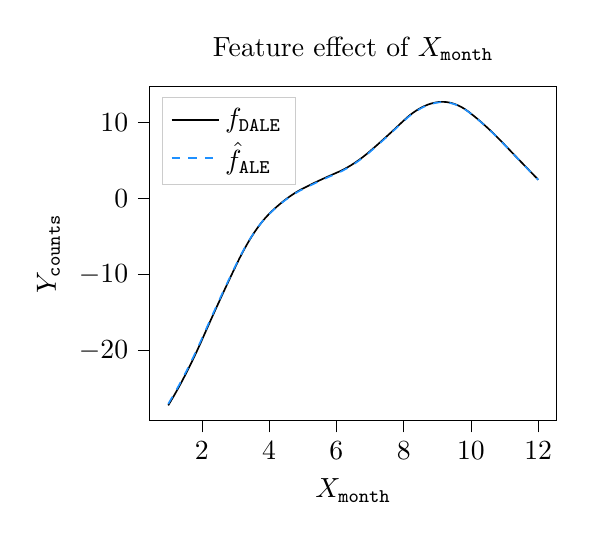
\begin{tikzpicture}

\definecolor{darkgray176}{RGB}{176,176,176}
\definecolor{dodgerblue}{RGB}{30,144,255}
\definecolor{lightgray204}{RGB}{204,204,204}

\begin{axis}[
legend cell align={left},
legend style={
  fill opacity=0.8,
  draw opacity=1,
  text opacity=1,
  at={(0.03,0.97)},
  anchor=north west,
  draw=lightgray204
},
tick align=outside,
tick pos=left,
title={Feature effect of \(\displaystyle X_{\mathtt{month}}\)},
x grid style={darkgray176},
xlabel={\(\displaystyle X_{\mathtt{month}}\)},
xmin=0.45, xmax=12.55,
xtick style={color=black},
y grid style={darkgray176},
ylabel={\(\displaystyle Y_{\mathtt{counts}}\)},
ymin=-29.183798458369, ymax=14.7468616660552,
ytick style={color=black}
]
\addplot [semithick, black]
table {%
1 -27.1869506835938
1.17617619037628 -25.871150970459
1.29729723930359 -24.9201946258545
1.40740740299225 -24.0201549530029
1.51751756668091 -23.0867099761963
1.63863861560822 -22.0221939086914
1.74874877929688 -21.0186061859131
1.85885882377625 -19.9816131591797
1.9689689874649 -18.9112167358398
2.09009003639221 -17.6963996887207
2.32132124900818 -15.3969707489014
2.64064073562622 -12.2988424301147
2.87187194824219 -10.1101322174072
3.1141140460968 -7.87898731231689
3.24624633789062 -6.75733757019043
3.35635638237 -5.88665103912354
3.45545554161072 -5.15343141555786
3.56556558609009 -4.3964409828186
3.67567563056946 -3.69928789138794
3.77477478981018 -3.12166857719421
3.88488483428955 -2.53821158409119
3.99499487876892 -2.01459169387817
4.13813829421997 -1.40747404098511
4.23723745346069 -1.0118283033371
4.34734725952148 -0.59662914276123
4.45745754241943 -0.207057595252991
4.56756734848022 0.156886339187622
4.66666650772095 0.462822675704956
4.7767767906189 0.778071641921997
4.88688707351685 1.06769299507141
4.98598575592041 1.30698728561401
5.21721744537354 1.81831657886505
5.43743753433228 2.28735709190369
5.64664649963379 2.71674489974976
5.86686706542969 3.15148568153381
6.12012004852295 3.64487433433533
6.19719696044922 3.81250214576721
6.30730724334717 4.07315158843994
6.42842864990234 4.38769626617432
6.53853845596313 4.69808197021484
6.64864873886108 5.03215312957764
6.75875854492188 5.3899097442627
6.87987995147705 5.81102657318115
6.98998975753784 6.21852016448975
7.23223209381104 7.15501070022583
7.463463306427 8.071533203125
7.6836838722229 8.96508026123047
7.90390396118164 9.87869548797607
8.09109115600586 10.6491012573242
8.17917919158936 10.9760904312134
8.27827835083008 11.3111982345581
8.38838863372803 11.6416292190552
8.49849891662598 11.9293622970581
8.60860824584961 12.1743965148926
8.70770740509033 12.3600397109985
8.81781768798828 12.5239429473877
8.92792797088623 12.6451482772827
9.03803825378418 12.7230014801025
9.1371374130249 12.7500133514404
9.17016983032227 12.7448768615723
9.24724769592285 12.7297611236572
9.28028011322021 12.7090911865234
9.35735702514648 12.6578493118286
9.40140151977539 12.6091642379761
9.47847843170166 12.5178241729736
9.58858871459961 12.3373823165894
9.69869899749756 12.1052808761597
9.80880928039551 11.8215208053589
9.92992973327637 11.4478168487549
10.1061058044434 10.8241405487061
10.2162160873413 10.4159374237061
10.3263263702393 9.99349880218506
10.4364366531372 9.55682373046875
10.5575571060181 9.06051921844482
10.667667388916 8.59395122528076
10.777777671814 8.11314868927002
10.8988990783691 7.56844854354858
11.7247247695923 3.76278614997864
12 2.50704598426819
};
\addlegendentry{$f_{\mathtt{DALE}}$}
\addplot [semithick, dodgerblue, dashed]
table {%
1 -27.0010604858398
1.18718719482422 -25.586950302124
1.29729723930359 -24.7142314910889
1.40740740299225 -23.809778213501
1.52852857112885 -22.77903175354
1.63863861560822 -21.8079357147217
1.74874877929688 -20.8051052093506
1.86986982822418 -19.666467666626
1.99099099636078 -18.4894695281982
2.2992992401123 -15.4285402297974
2.51951956748962 -13.2975368499756
2.72872877120972 -11.3166017532349
2.94894886016846 -9.27656745910645
3.1141140460968 -7.78738117218018
3.24624633789062 -6.68413352966309
3.35635638237 -5.82812023162842
3.45545554161072 -5.10758543014526
3.56556558609009 -4.36409330368042
3.67567563056946 -3.67981958389282
3.77477478981018 -3.113276720047
3.88488483428955 -2.54152417182922
3.99499487876892 -2.02899026870728
4.13813829421997 -1.43530428409576
4.23723745346069 -1.04830312728882
4.34734725952148 -0.642061471939087
4.45745754241943 -0.260767459869385
4.56756734848022 0.0955789089202881
4.66666650772095 0.395250797271729
4.7767767906189 0.704194068908691
4.88688707351685 0.988189816474915
4.98598575592041 1.22298789024353
5.23923921585083 1.77311503887177
5.4484486579895 2.21300554275513
5.66866874694824 2.66170525550842
5.88888883590698 3.09569883346558
6.10910892486572 3.52712678909302
6.19719696044922 3.71933627128601
6.30730724334717 3.9817156791687
6.42842864990234 4.29802989959717
6.53853845596313 4.60990715026855
6.64864873886108 4.9453558921814
6.75875854492188 5.30437612533569
6.87987995147705 5.72675085067749
6.98998975753784 6.13526916503906
7.24324321746826 7.11681127548218
7.463463306427 7.99168014526367
7.6836838722229 8.8862886428833
7.90390396118164 9.80063629150391
8.09109115600586 10.5716905593872
8.17917919158936 10.899432182312
8.2892894744873 11.2697401046753
8.38838863372803 11.5681610107422
8.49849891662598 11.8583631515503
8.60860824584961 12.106406211853
8.70770740509033 12.2951984405518
8.81781768798828 12.463134765625
8.92792797088623 12.5889139175415
9.03803825378418 12.6718053817749
9.1371374130249 12.702956199646
9.17016983032227 12.6990699768066
9.24724769592285 12.6868410110474
9.28028011322021 12.6672773361206
9.35735702514648 12.6185913085938
9.40140151977539 12.5711889266968
9.47847843170166 12.4820346832275
9.58858871459961 12.3042573928833
9.69869899749756 12.0743465423584
9.80880928039551 11.7923011779785
9.92992973327637 11.4199190139771
10.1061058044434 10.7974834442139
10.2162160873413 10.3899793624878
10.3263263702393 9.96817970275879
10.4364366531372 9.53208541870117
10.5575571060181 9.03635120391846
10.667667388916 8.57023906707764
10.777777671814 8.08983135223389
10.8988990783691 7.54549980163574
11.7027025222778 3.84338307380676
12 2.48848509788513
};
\addlegendentry{$\hat{f}_{\mathtt{ALE}}$}
\end{axis}

\end{tikzpicture}
}
  \resizebox{.3\columnwidth}{!}{% This file was created with tikzplotlib v0.10.1.
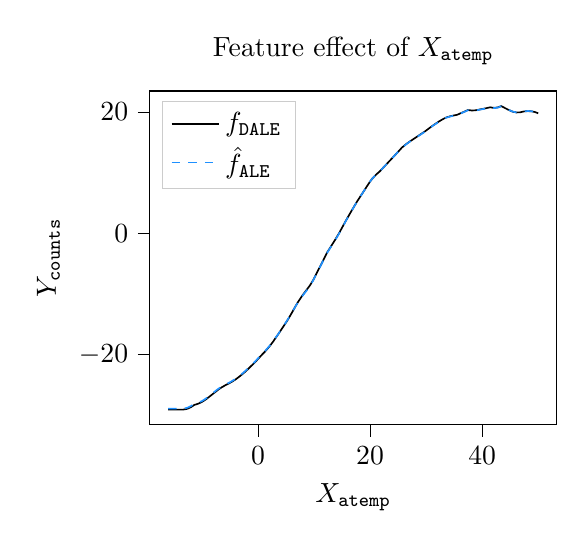
\begin{tikzpicture}

\definecolor{darkgray176}{RGB}{176,176,176}
\definecolor{dodgerblue}{RGB}{30,144,255}
\definecolor{lightgray204}{RGB}{204,204,204}

\begin{axis}[
legend cell align={left},
legend style={
  fill opacity=0.8,
  draw opacity=1,
  text opacity=1,
  at={(0.03,0.97)},
  anchor=north west,
  draw=lightgray204
},
tick align=outside,
tick pos=left,
title={Feature effect of \(\displaystyle X_{\mathtt{atemp}}\)},
x grid style={darkgray176},
xlabel={\(\displaystyle X_{\mathtt{atemp}}\)},
xmin=-19.3, xmax=53.3,
xtick style={color=black},
y grid style={darkgray176},
ylabel={\(\displaystyle Y_{\mathtt{counts}}\)},
ymin=-31.6301535780892, ymax=23.4795271752803,
ytick style={color=black}
]
\addplot [semithick, black]
table {%
-16 -29.1201610565186
-14.5465469360352 -29.1236610412598
-13.3573570251465 -29.1187324523926
-12.6306304931641 -28.9887657165527
-11.9699697494507 -28.7167987823486
-11.3753757476807 -28.351110458374
-10.5825824737549 -28.10817527771
-9.9219217300415 -27.8089466094971
-9.26126098632812 -27.4157428741455
-8.13813781738281 -26.5979690551758
-6.94894886016846 -25.7284774780273
-6.55255270004272 -25.4859237670898
-5.89189195632935 -25.1317119598389
-4.70270252227783 -24.557861328125
-3.90990996360779 -24.0795192718506
-3.11711716651917 -23.5240688323975
-2.52252244949341 -23.0663394927979
-1.86186182498932 -22.5092353820801
-0.540540456771851 -21.3122959136963
0.120120167732239 -20.6509094238281
0.714714765548706 -20.0558643341064
1.30930936336517 -19.4900760650635
2.03603601455688 -18.7049884796143
2.63063073158264 -17.9895362854004
3.8858859539032 -16.3134365081787
5.27327346801758 -14.3682708740234
6 -13.2194204330444
6.85885906219482 -11.8082704544067
7.25525522232056 -11.203857421875
7.91591596603394 -10.3020009994507
9.30330371856689 -8.58228397369385
9.83183193206787 -7.77181529998779
10.9549551010132 -5.72904586791992
12.342342376709 -3.19349336624146
12.5405406951904 -2.89349699020386
13.7957954406738 -1.05008816719055
14.4564561843872 -0.0256915092468262
15.6456460952759 2.00035262107849
16.5705699920654 3.49347949028015
17.6936931610107 5.24578619003296
19.9399394989014 8.44653511047363
20.4024028778076 9.01027202606201
21.0630626678467 9.66129207611084
21.7237243652344 10.1941547393799
24.8948955535889 13.3221054077148
25.687686920166 14.134651184082
26.4804801940918 14.7308025360107
27.1411418914795 15.1683645248413
29.8498497009277 16.8362903594971
30.7087078094482 17.4392356872559
31.3693695068359 17.8697376251221
32.3603591918945 18.484224319458
33.087085723877 18.8724536895752
33.5495491027832 19.0880432128906
34.4084091186523 19.3274822235107
35.0690689086914 19.4596900939941
35.5315322875977 19.543493270874
36.9849853515625 20.1296157836914
37.4474487304688 20.3274917602539
37.6456451416016 20.3095550537109
38.1741752624512 20.2521419525146
38.8348350524902 20.287296295166
39.8258247375488 20.4710922241211
40.6186180114746 20.6114158630371
41.345344543457 20.7675323486328
41.4114112854004 20.7821464538574
41.8078079223633 20.7240734100342
42.1381378173828 20.6876392364502
42.7987976074219 20.7667903900146
43.3933944702148 20.9745426177979
43.657657623291 20.8512020111084
44.714714050293 20.3551597595215
45.4414405822754 20.057201385498
46.1021003723145 19.9324207305908
46.7627639770508 19.9523639678955
47.4894905090332 20.1014881134033
48.1501502990723 20.1500225067139
48.8108100891113 20.1130447387695
49.4054069519043 20.0048065185547
50 19.7889881134033
};
\addlegendentry{$f_{\mathtt{DALE}}$}
\addplot [semithick, dodgerblue, dashed]
table {%
-16 -28.9542388916016
-14.5465469360352 -28.9578762054443
-13.3573570251465 -28.9526977539062
-12.6306304931641 -28.8202018737793
-11.9699697494507 -28.5466842651367
-11.3753757476807 -28.1803741455078
-10.6486482620239 -27.9906787872314
-9.98798751831055 -27.7104911804199
-9.26126098632812 -27.2779521942139
-8.00600624084473 -26.3645648956299
-7.2132134437561 -25.7814712524414
-6.55255270004272 -25.3670864105225
-5.89189195632935 -25.0190086364746
-4.76876878738403 -24.4896812438965
-3.90990996360779 -23.9704494476318
-3.05105113983154 -23.364631652832
-2.52252244949341 -22.9567375183105
-1.86186182498932 -22.4021339416504
-0.606606602668762 -21.2720623016357
0.120120167732239 -20.5483741760254
0.648648619651794 -20.0188083648682
1.30930936336517 -19.4072608947754
1.96996998786926 -18.7101631164551
2.69669675827026 -17.8467922210693
3.55555558204651 -16.7303333282471
4.21621608734131 -15.8174858093262
5.53753757476807 -13.9267387390137
6 -13.1932601928711
6.66066074371338 -12.1299390792847
7.32132148742676 -11.1632461547852
7.91591596603394 -10.3738870620728
8.97297286987305 -9.1130838394165
9.10510540008545 -8.9506664276123
9.83183193206787 -7.83912706375122
11.2852849960327 -5.17018270492554
12.408408164978 -3.13905572891235
13.5975971221924 -1.41476833820343
14.3243246078491 -0.306623458862305
14.6546545028687 0.264089107513428
15.6456460952759 1.96240651607513
16.5705699920654 3.46715188026428
17.6936931610107 5.24065256118774
19.8738746643066 8.35614967346191
20.4024028778076 9.0117301940918
21.0630626678467 9.66457653045654
21.7237243652344 10.1938533782959
25.4894886016846 13.9263477325439
25.6216220855713 14.053521156311
26.4804801940918 14.7064094543457
27.1411418914795 15.1473188400269
29.057056427002 16.3006134033203
29.6516513824463 16.6701507568359
30.6426429748535 17.3715686798096
31.2372379302979 17.7557601928711
32.4924926757812 18.524055480957
33.087085723877 18.8392581939697
33.5495491027832 19.0558605194092
34.4084091186523 19.2951412200928
35.0690689086914 19.4283008575439
35.5315322875977 19.5130195617676
36.9849853515625 20.0959377288818
37.4474487304688 20.291877746582
37.6456451416016 20.2738914489746
38.1741752624512 20.216480255127
38.8348350524902 20.2516288757324
39.8258247375488 20.4354114532471
40.6186180114746 20.5759296417236
41.2792778015137 20.7178859710693
41.4114112854004 20.7472190856934
41.8078079223633 20.6907978057861
42.1381378173828 20.6556282043457
42.7987976074219 20.7358493804932
43.3933944702148 20.9432563781738
43.657657623291 20.8323345184326
45.375373840332 20.0885391235352
46.0360374450684 19.9492740631104
46.6966972351074 19.9548187255859
47.5555572509766 20.1251811981201
48.1501502990723 20.1673374176025
48.8108100891113 20.1304454803467
49.4054069519043 20.0222206115723
50 19.8063983917236
};
\addlegendentry{$\hat{f}_{\mathtt{ALE}}$}
\end{axis}

\end{tikzpicture}
}
  \resizebox{.3\columnwidth}{!}{% This file was created with tikzplotlib v0.10.1.
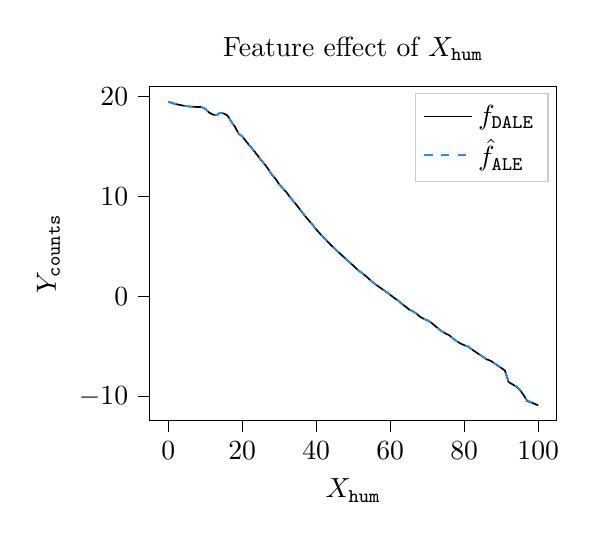
\begin{tikzpicture}

\definecolor{darkgray176}{RGB}{176,176,176}
\definecolor{dodgerblue}{RGB}{30,144,255}
\definecolor{lightgray204}{RGB}{204,204,204}

\begin{axis}[
legend cell align={left},
legend style={fill opacity=0.8, draw opacity=1, text opacity=1, draw=lightgray204},
tick align=outside,
tick pos=left,
title={Feature effect of \(\displaystyle X_{\mathtt{hum}}\)},
x grid style={darkgray176},
xlabel={\(\displaystyle X_{\mathtt{hum}}\)},
xmin=-5, xmax=105,
xtick style={color=black},
y grid style={darkgray176},
ylabel={\(\displaystyle Y_{\mathtt{counts}}\)},
ymin=-12.4017583163331, ymax=20.9680093156312,
ytick style={color=black}
]
\addplot [semithick, black]
table {%
0 19.445671081543
1.80180180072784 19.2508811950684
2.8028028011322 19.1621017456055
3.80380392074585 19.0876598358154
4.80480480194092 19.0275573730469
5.80580568313599 18.9817924499512
6.80680704116821 18.9503650665283
7.80780792236328 18.933277130127
8.80880928039551 18.9305267333984
9.00900936126709 18.9289054870605
10.010009765625 18.7470264434814
11.0110111236572 18.3885173797607
12.0120124816895 18.1801509857178
13.0130128860474 18.1236801147461
14.0140142440796 18.3442001342773
15.0150146484375 18.2827415466309
16.0160160064697 18.0843563079834
17.1171169281006 17.4235782623291
18.0180187225342 16.9714221954346
19.0190181732178 16.268253326416
20.02001953125 15.9827404022217
21.2212219238281 15.4168157577515
23.2232227325439 14.5354175567627
24.4244251251221 13.9460258483887
25.325325012207 13.5335330963135
26.2262268066406 13.1304426193237
27.027027130127 12.738260269165
28.0280284881592 12.1465797424316
29.0290298461914 11.7472257614136
30.030029296875 11.1805286407471
31.9319324493408 10.4186792373657
32.1321334838867 10.3230867385864
33.033031463623 9.86366176605225
34.1341323852539 9.40140438079834
36.9369354248047 8.0537805557251
37.4374389648438 7.83730363845825
39.2392387390137 7.05814123153687
40.1401405334473 6.63687181472778
41.5415420532227 6.06709289550781
42.5425415039062 5.68619441986084
43.3433418273926 5.3793511390686
44.1441459655762 5.07060098648071
45.1451454162598 4.7441782951355
46.2462463378906 4.34106254577637
50.1501502990723 3.03945064544678
51.1511497497559 2.67909049987793
52.352352142334 2.33571791648865
53.1531524658203 2.11605978012085
54.5545539855957 1.6564826965332
55.1551551818848 1.46061563491821
56.6566581726074 1.04154002666473
58.0580596923828 0.674215078353882
59.4594612121582 0.312742352485657
60.4604606628418 0.0281145572662354
61.1611595153809 -0.170746326446533
62.0620613098145 -0.390427708625793
63.1631622314453 -0.749048829078674
64.1641616821289 -1.0204029083252
65.0650634765625 -1.29337751865387
66.1661682128906 -1.49768507480621
67.0670700073242 -1.71112847328186
68.0680694580078 -2.03258061408997
69.0690689086914 -2.23863196372986
70.070068359375 -2.38389420509338
71.0710678100586 -2.61734461784363
73.3733749389648 -3.33057689666748
74.1741714477539 -3.53978538513184
75.175178527832 -3.74607062339783
75.9759750366211 -3.88061666488647
76.3763732910156 -4.00896739959717
77.1771774291992 -4.26187658309937
78.2782745361328 -4.54429483413696
79.0790786743164 -4.72437953948975
80.1801834106445 -4.89549112319946
80.9809799194336 -4.98908805847168
81.3813781738281 -5.09695863723755
82.8828811645508 -5.50094985961914
83.5835800170898 -5.67414093017578
84.584587097168 -5.90682792663574
85.185188293457 -6.05287551879883
85.9859848022461 -6.28149127960205
86.4864883422852 -6.34115266799927
87.0870895385742 -6.42070388793945
88.6886901855469 -6.81395483016968
90.9909896850586 -7.4021258354187
91.2912902832031 -7.73944664001465
91.9919891357422 -8.54510974884033
92.1921920776367 -8.59602737426758
94.0940933227539 -9.01366710662842
94.9949951171875 -9.32887077331543
95.9959945678711 -9.81900787353516
96.9969940185547 -10.4498987197876
97.7977981567383 -10.5560169219971
98.7987976074219 -10.6977682113647
99.7997970581055 -10.85329246521
100 -10.8849506378174
};
\addlegendentry{$f_{\mathtt{DALE}}$}
\addplot [semithick, dodgerblue, dashed]
table {%
0 19.4512023925781
1.80180180072784 19.2567539215088
2.8028028011322 19.1681327819824
3.80380392074585 19.093822479248
4.80480480194092 19.0338249206543
5.80580568313599 18.9881401062012
6.80680704116821 18.9567699432373
7.80780792236328 18.9397106170654
8.80880928039551 18.9369659423828
9.00900936126709 18.9353446960449
10.010009765625 18.753490447998
11.0110111236572 18.3950309753418
12.0120124816895 18.1866893768311
13.0130128860474 18.1302185058594
14.0140142440796 18.3507404327393
15.0150146484375 18.289701461792
16.0160160064697 18.0913181304932
17.1171169281006 17.4305477142334
18.0180187225342 16.9784984588623
19.0190181732178 16.2804527282715
20.02001953125 15.9955158233643
21.2212219238281 15.4311323165894
23.1231231689453 14.5908050537109
24.3243236541748 13.9988222122192
25.325325012207 13.5421257019043
26.1261253356934 13.187403678894
27.027027130127 12.7418575286865
28.0280284881592 12.1519727706909
29.0290298461914 11.7499494552612
30.030029296875 11.182975769043
32.0320320129395 10.3707160949707
33.033031463623 9.85312747955322
34.1341323852539 9.38883113861084
36.6366348266602 8.18614196777344
37.1371383666992 7.95634317398071
39.0390396118164 7.15220594406128
40.1401405334473 6.63696813583374
41.4414405822754 6.10159015655518
42.4424438476562 5.71701908111572
43.3433418273926 5.37234306335449
44.1441459655762 5.06235647201538
45.1451454162598 4.73639726638794
46.2462463378906 4.33528661727905
50.050048828125 3.06395077705383
51.1511497497559 2.66571760177612
52.2522506713867 2.34696483612061
53.1531524658203 2.10619187355042
54.5545539855957 1.64742040634155
55.1551551818848 1.4514753818512
56.5565567016602 1.06200659275055
58.1581573486328 0.648456811904907
59.4594612121582 0.313627243041992
60.4604606628418 0.0284990072250366
61.1611595153809 -0.170641422271729
62.0620613098145 -0.391844630241394
63.0630645751953 -0.725825071334839
64.2642669677734 -1.05191004276276
65.0650634765625 -1.28894066810608
66.1661682128906 -1.49367189407349
67.0670700073242 -1.70696103572845
68.0680694580078 -2.03458189964294
69.0690689086914 -2.24001359939575
70.070068359375 -2.38448262214661
71.0710678100586 -2.62038135528564
73.2732696533203 -3.31713366508484
74.1741714477539 -3.55359435081482
75.175178527832 -3.7575466632843
75.9759750366211 -3.88404536247253
76.2762756347656 -3.97914242744446
77.1771774291992 -4.2657265663147
78.2782745361328 -4.54978799819946
79.1791763305664 -4.74476099014282
80.1801834106445 -4.89946508407593
80.9809799194336 -4.99041557312012
81.3813781738281 -5.09758758544922
82.9829864501953 -5.52745628356934
84.2842864990234 -5.83696460723877
85.185188293457 -6.04725694656372
85.9859848022461 -6.27391958236694
86.4864883422852 -6.33382940292358
87.0870895385742 -6.41337013244629
88.6886901855469 -6.80084180831909
90.9909896850586 -7.36907291412354
91.2912902832031 -7.70228242874146
91.9919891357422 -8.49856758117676
92.1921920776367 -8.5493803024292
94.0940933227539 -8.96699905395508
94.9949951171875 -9.28218460083008
95.9959945678711 -9.77230548858643
96.9969940185547 -10.4031848907471
97.7977981567383 -10.509295463562
98.5986022949219 -10.6244306564331
99.5996017456055 -10.7833385467529
100 -10.8497257232666
};
\addlegendentry{$\hat{f}_{\mathtt{ALE}}$}
\end{axis}

\end{tikzpicture}
}
  \caption{Bike-Sharing Dataset. DALE and ALE feature effect plots with \(K=200\) for:
    \(X_{\texttt{month}}\), \(X_{\mathtt{atemp}}\),\(X_{\mathtt{hum}}\).}
  \label{fig:bike-sharing-comparison}
\end{figure}


\begin{figure}[h]
  \centering
    \resizebox{.3\columnwidth}{!}{% This file was created with tikzplotlib v0.10.1.
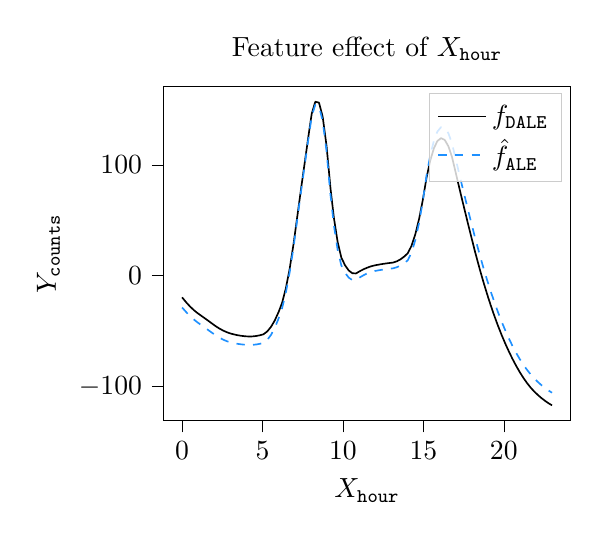
\begin{tikzpicture}

\definecolor{darkgray176}{RGB}{176,176,176}
\definecolor{dodgerblue}{RGB}{30,144,255}
\definecolor{lightgray204}{RGB}{204,204,204}

\begin{axis}[
legend cell align={left},
legend style={fill opacity=0.8, draw opacity=1, text opacity=1, draw=lightgray204},
tick align=outside,
tick pos=left,
title={Feature effect of \(\displaystyle X_{\mathtt{hour}}\)},
x grid style={darkgray176},
xlabel={\(\displaystyle X_{\mathtt{hour}}\)},
xmin=-1.15, xmax=24.15,
xtick style={color=black},
y grid style={darkgray176},
ylabel={\(\displaystyle Y_{\mathtt{counts}}\)},
ymin=-130.55351264475, ymax=170.472616656964,
ytick style={color=black}
]
\addplot [semithick, black]
table {%
0 -19.5050849914551
0.276276350021362 -24.3441772460938
0.506506443023682 -27.9236030578613
0.73673677444458 -31.0645523071289
0.943943977355957 -33.5316467285156
1.54254257678986 -39.7169952392578
2.00300312042236 -44.5988159179688
2.11811804771423 -45.7644081115723
2.32532525062561 -47.663459777832
2.55555558204651 -49.4630393981934
2.78578567504883 -50.9483070373535
2.99299287796021 -52.0300178527832
3.24624633789062 -52.9924545288086
3.47647643089294 -53.6967239379883
3.68368363380432 -54.1934471130371
3.91391396522522 -54.5767364501953
4.14414405822754 -54.7889671325684
4.37437438964844 -54.7139015197754
4.60460472106934 -54.3515357971191
4.83483505249023 -53.7018775939941
5.04204225540161 -52.8642959594727
5.06506490707397 -52.7370185852051
5.29529523849487 -50.2154121398926
5.52552556991577 -46.1370544433594
5.75575590133667 -40.5019493103027
6.00900888442993 -32.4394378662109
6.21621608734131 -24.4946517944336
6.44644641876221 -11.6443128585815
6.67667675018311 5.24092245101929
6.92992973327637 28.6440601348877
7.43643665313721 82.6207962036133
7.89689683914185 130.067947387695
8.05805778503418 145.936157226562
8.26526546478271 156.092514038086
8.28828811645508 156.789611816406
8.49549579620361 156.161087036133
8.51851844787598 155.647872924805
8.72572612762451 144.234481811523
8.74874877929688 142.510955810547
8.97897911071777 117.378860473633
9.23223209381104 78.1012954711914
9.43943977355957 52.0760345458984
9.66967010498047 30.5269412994385
9.89989948272705 16.3793964385986
10.1301298141479 9.40791988372803
10.3603601455688 4.70836496353149
10.5675678253174 2.42953133583069
10.5905904769897 2.28073143959045
10.7977981567383 2.04458355903625
10.8208208084106 2.12501859664917
11.0740737915039 4.29217100143433
11.3043041229248 5.98237943649292
11.5345344543457 7.39637041091919
11.7417421340942 8.44379425048828
11.9719715118408 9.33294486999512
12.2482481002808 10.0710592269897
12.4784784317017 10.624490737915
12.7087087631226 11.1187515258789
12.9159154891968 11.5147294998169
13.1001005172729 11.8276166915894
13.1231231689453 11.9058475494385
13.3303298950195 12.875524520874
13.3763761520386 13.199444770813
13.5835838317871 14.8272914886475
13.813814163208 17.3185062408447
14.0210208892822 20.1412181854248
14.0670671463013 21.3190975189209
14.2512512207031 26.5641231536865
14.2972974777222 28.4294090270996
14.5045042037964 37.6234588623047
14.7347345352173 51.2384872436523
14.9649648666382 68.2768707275391
15.1951951980591 88.2222595214844
15.42542552948 103.759735107422
15.6556558609009 114.889282226562
15.8628625869751 121.212203979492
15.8858861923218 121.610908508301
16.0930938720703 123.970664978027
16.1161155700684 123.936637878418
16.3233242034912 122.487854003906
16.3693695068359 121.442276000977
16.5535526275635 116.769096374512
16.6226234436035 113.865631103516
16.7837829589844 106.814399719238
16.8758754730225 101.206695556641
17.3363361358643 72.9654541015625
17.7967967987061 45.5679664611816
18.2112121582031 21.7020950317383
18.5105113983154 5.64360857009888
18.7407398223877 -5.97945785522461
18.9709701538086 -16.9456024169922
19.1781787872314 -26.2628364562988
19.4084091186523 -35.9988479614258
19.6386394500732 -45.0910110473633
19.8688697814941 -53.5393295288086
20.0990982055664 -61.3896484375
20.3293285369873 -68.7146987915039
20.5365371704102 -74.8665542602539
20.7667675018311 -81.1935348510742
20.996997833252 -86.995246887207
21.2042045593262 -91.7762222290039
21.4344348907471 -96.5489959716797
21.664665222168 -100.770584106445
21.8948955535889 -104.44100189209
22.1481475830078 -107.900184631348
22.3553562164307 -110.46851348877
22.5855846405029 -113.02222442627
22.8158149719238 -115.269233703613
23 -116.870506286621
};
\addlegendentry{$f_{\mathtt{DALE}}$}
\addplot [semithick, dodgerblue, dashed]
table {%
0 -28.6461296081543
0.299299240112305 -33.4844398498535
0.506506443023682 -36.5122833251953
0.73673677444458 -39.5242080688477
0.966966986656189 -42.1757049560547
1.74974977970123 -50.2825317382812
2.11811804771423 -54.0799827575684
2.32532525062561 -55.9247512817383
2.55555558204651 -57.6483955383301
2.78578567504883 -59.0419044494629
2.99299287796021 -60.0281982421875
3.24624633789062 -60.8593711853027
3.47647643089294 -61.46630859375
3.68368363380432 -61.8931121826172
3.91391396522522 -62.2204475402832
4.14414405822754 -62.3986968994141
4.37437438964844 -62.3219032287598
4.60460472106934 -61.990062713623
4.83483505249023 -61.4031791687012
5.04204225540161 -60.6504898071289
5.06506490707397 -60.5277214050293
5.29529523849487 -57.8714256286621
5.52552556991577 -53.4342956542969
5.75575590133667 -47.2163352966309
6.00900888442993 -38.2443809509277
6.21621608734131 -29.381742477417
6.44644641876221 -15.6827802658081
6.69969987869263 4.01029825210571
6.92992973327637 25.8215217590332
7.39039039611816 75.5200271606445
7.85085105895996 123.192329406738
8.05805778503418 143.596130371094
8.26526546478271 153.462203979492
8.28828811645508 154.119873046875
8.49549579620361 153.021850585938
8.51851844787598 152.449096679688
8.72572612762451 140.386978149414
8.74874877929688 138.58381652832
8.97897911071777 112.524017333984
9.20920944213867 75.0672760009766
9.43943977355957 45.3751182556152
9.66967010498047 23.4475517272949
9.89989948272705 9.28457546234131
10.1301298141479 2.64411807060242
10.3603601455688 -1.73881900310516
10.5675678253174 -3.74506211280823
10.5905904769897 -3.86423587799072
10.7977981567383 -3.84074091911316
10.8208208084106 -3.73213291168213
11.0740737915039 -1.27214574813843
11.3043041229248 0.624772906303406
11.5115118026733 2.059002161026
11.7417421340942 3.31951761245728
11.9719715118408 4.24510145187378
12.2482481002808 4.96000051498413
12.4784784317017 5.49322175979614
12.7087087631226 5.96644258499146
12.9159154891968 6.34280109405518
13.1001005172729 6.63770151138306
13.1231231689453 6.70726346969604
13.3303298950195 7.55532884597778
13.3763761520386 7.83442735671997
13.5835838317871 9.23264122009277
13.813814163208 11.3566951751709
14.0210208892822 13.7536668777466
14.0440444946289 14.2715625762939
14.2512512207031 20.38014793396
14.2972974777222 22.4057006835938
14.5045042037964 32.4857139587402
14.7347345352173 47.7849960327148
14.9649648666382 67.2124176025391
15.1951951980591 90.178352355957
15.42542552948 108.329772949219
15.6556558609009 121.666687011719
15.8628625869751 129.635528564453
15.9089088439941 130.593536376953
16.0930938720703 133.829193115234
16.1161155700684 133.91423034668
16.3233242034912 133.447540283203
16.3463459014893 133.071701049805
16.5535526275635 128.498184204102
16.5995998382568 126.696998596191
16.7837829589844 118.981163024902
16.8758754730225 113.421195983887
17.3363361358643 85.3754196166992
17.7967967987061 58.1768074035645
18.2112121582031 34.4831466674805
18.5335330963135 17.2674236297607
18.7407398223877 6.80826711654663
18.9709701538086 -4.24147033691406
19.2012004852295 -14.6806631088257
19.4084091186523 -23.5517692565918
19.6386394500732 -32.8170890808105
19.8688697814941 -41.4646186828613
20.0990982055664 -49.5049858093262
20.3063068389893 -56.2461433410645
20.5365371704102 -63.1648941040039
20.7667675018311 -69.4933547973633
20.9739742279053 -74.6995239257812
21.2272281646729 -80.4064331054688
21.4344348907471 -84.651123046875
21.664665222168 -88.8804550170898
21.8948955535889 -92.6121520996094
22.1481475830078 -96.1844940185547
22.3553562164307 -98.8407440185547
22.5855846405029 -101.486793518066
22.8158149719238 -103.820686340332
23 -105.487968444824
};
\addlegendentry{$\hat{f}_{\mathtt{ALE}}$}
\end{axis}

\end{tikzpicture}
}
    \resizebox{.3\columnwidth}{!}{% This file was created with tikzplotlib v0.10.1.
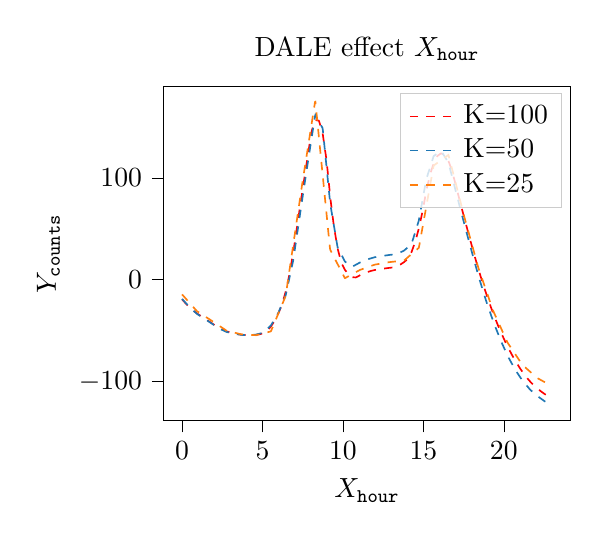
\begin{tikzpicture}

\definecolor{darkgray176}{RGB}{176,176,176}
\definecolor{darkorange25512714}{RGB}{255,127,14}
\definecolor{lightgray204}{RGB}{204,204,204}
\definecolor{steelblue31119180}{RGB}{31,119,180}

\begin{axis}[
legend cell align={left},
legend style={fill opacity=0.8, draw opacity=1, text opacity=1, draw=lightgray204},
tick align=outside,
tick pos=left,
title={DALE effect \(\displaystyle X_{\mathtt{hour}}\)},
x grid style={darkgray176},
xlabel={\(\displaystyle X_{\mathtt{hour}}\)},
xmin=-1.15, xmax=24.15,
xtick style={color=black},
y grid style={darkgray176},
ylabel={\(\displaystyle Y_{\mathtt{counts}}\)},
ymin=-138.606064986267, ymax=189.589636529361,
ytick style={color=black}
]
\addplot [semithick, red, dashed]
table {%
0 -19.5050849914551
0.276276350021362 -24.3441772460938
0.506506443023682 -27.9236030578613
0.73673677444458 -31.0645523071289
0.943943977355957 -33.5316467285156
1.54254257678986 -39.7169952392578
2.00300312042236 -44.5988159179688
2.11811804771423 -45.7644081115723
2.32532525062561 -47.663459777832
2.55555558204651 -49.4630393981934
2.78578567504883 -50.9483070373535
2.99299287796021 -52.0300178527832
3.24624633789062 -52.9924545288086
3.47647643089294 -53.6967239379883
3.68368363380432 -54.1934471130371
3.91391396522522 -54.5767364501953
4.14414405822754 -54.7889671325684
4.37437438964844 -54.7139015197754
4.60460472106934 -54.3515357971191
4.83483505249023 -53.7018775939941
5.04204225540161 -52.8642959594727
5.06506490707397 -52.7370185852051
5.29529523849487 -50.2154121398926
5.52552556991577 -46.1370544433594
5.75575590133667 -40.5019493103027
6.00900888442993 -32.4394378662109
6.21621608734131 -24.4946517944336
6.44644641876221 -11.6443128585815
6.67667675018311 5.24092245101929
6.92992973327637 28.6440601348877
7.43643665313721 82.6207962036133
7.89689683914185 130.067947387695
8.05805778503418 145.936157226562
8.26526546478271 156.092514038086
8.28828811645508 156.789611816406
8.49549579620361 156.161087036133
8.51851844787598 155.647872924805
8.72572612762451 144.234481811523
8.74874877929688 142.510955810547
8.97897911071777 117.378860473633
9.23223209381104 78.1012954711914
9.43943977355957 52.0760345458984
9.66967010498047 30.5269412994385
9.89989948272705 16.3793964385986
10.1301298141479 9.40791988372803
10.3603601455688 4.70836496353149
10.5675678253174 2.42953133583069
10.5905904769897 2.28073143959045
10.7977981567383 2.04458355903625
10.8208208084106 2.12501859664917
11.0740737915039 4.29217100143433
11.3043041229248 5.98237943649292
11.5345344543457 7.39637041091919
11.7417421340942 8.44379425048828
11.9719715118408 9.33294486999512
12.2482481002808 10.0710592269897
12.4784784317017 10.624490737915
12.7087087631226 11.1187515258789
12.9159154891968 11.5147294998169
13.1001005172729 11.8276166915894
13.1231231689453 11.9058475494385
13.3303298950195 12.875524520874
13.3763761520386 13.199444770813
13.5835838317871 14.8272914886475
13.813814163208 17.3185062408447
14.0210208892822 20.1412181854248
14.0670671463013 21.3190975189209
14.2512512207031 26.5641231536865
14.2972974777222 28.4294090270996
14.5045042037964 37.6234588623047
14.7347345352173 51.2384872436523
14.9649648666382 68.2768707275391
15.1951951980591 88.2222595214844
15.42542552948 103.759735107422
15.6556558609009 114.889282226562
15.8628625869751 121.212203979492
15.8858861923218 121.610908508301
16.0930938720703 123.970664978027
16.1161155700684 123.936637878418
16.3233242034912 122.487854003906
16.3693695068359 121.442276000977
16.5535526275635 116.769096374512
16.6226234436035 113.865631103516
16.7837829589844 106.814399719238
16.8758754730225 101.206695556641
17.3363361358643 72.9654541015625
17.7967967987061 45.5679664611816
18.2112121582031 21.7020950317383
18.5105113983154 5.64360857009888
18.7407398223877 -5.97945785522461
18.9709701538086 -16.9456024169922
19.1781787872314 -26.2628364562988
19.4084091186523 -35.9988479614258
19.6386394500732 -45.0910110473633
19.8688697814941 -53.5393295288086
20.0990982055664 -61.3896484375
20.3293285369873 -68.7146987915039
20.5365371704102 -74.8665542602539
20.7667675018311 -81.1935348510742
20.996997833252 -86.995246887207
21.2042045593262 -91.7762222290039
21.4344348907471 -96.5489959716797
21.664665222168 -100.770584106445
21.8948955535889 -104.44100189209
22.1481475830078 -107.900184631348
22.3553562164307 -110.46851348877
22.5855846405029 -113.02222442627
22.8158149719238 -115.269233703613
23 -116.870506286621
};
\addlegendentry{K=100}
\addplot [semithick, steelblue31119180, dashed]
table {%
0 -19.0568523406982
0.483483552932739 -27.5899829864502
0.943943977355957 -33.9586143493652
1.65765762329102 -41.3208885192871
2.11811804771423 -46.2027359008789
2.30230236053467 -48.1648330688477
2.76276278495789 -51.5102844238281
3.2232232093811 -53.2904281616211
3.68368363380432 -54.3948593139648
4.12112092971802 -54.8079147338867
4.14414405822754 -54.8193206787109
4.60460472106934 -54.0945930480957
5.04204225540161 -52.3263702392578
5.06506490707397 -52.1762809753418
5.52552556991577 -45.0688095092773
5.98598575592041 -32.7721710205078
6.44644641876221 -15.1332197189331
6.906907081604 18.6453113555908
7.5515513420105 87.5196990966797
8.01201248168945 134.966445922852
8.26526546478271 160.561309814453
8.28828811645508 161.809616088867
8.72572612762451 149.098709106445
8.74874877929688 147.291305541992
9.20920944213867 74.5869293212891
9.66967010498047 31.4887447357178
10.1301298141479 17.5457916259766
10.5675678253174 12.734920501709
10.5905904769897 12.6905250549316
11.0510511398315 16.6829795837402
11.5115118026733 19.7547092437744
11.9719715118408 21.9057159423828
12.4554557800293 23.2053813934326
12.8928928375244 24.1664962768555
13.3303298950195 24.9096031188965
13.3533535003662 25.0283260345459
13.7907905578613 28.3794097900391
13.8368368148804 28.9517726898193
14.2512512207031 34.5971946716309
14.2742738723755 35.4409217834473
14.7117118835449 57.6446723937988
14.757758140564 61.3840827941895
15.1721725463867 97.8089218139648
15.2182178497314 100.394157409668
15.6326322555542 120.966339111328
15.6556558609009 121.510360717773
16.0930938720703 126.492065429688
16.1161155700684 126.161819458008
16.5535526275635 115.063018798828
16.5995998382568 112.439018249512
17.2672672271729 71.3320007324219
17.7277278900146 43.8025321960449
18.1881885528564 16.976188659668
18.4644641876221 1.44218516349792
18.9019012451172 -21.0025215148926
19.362361907959 -42.0182228088379
19.8228225708008 -60.4585456848145
20.2602596282959 -75.6445541381836
20.7207202911377 -89.0095443725586
21.1811809539795 -99.7675628662109
21.6416416168213 -108.320869445801
22.1021022796631 -114.716354370117
22.5625629425049 -119.885055541992
23 -123.688079833984
};
\addlegendentry{K=50}
\addplot [semithick, darkorange25512714, dashed]
table {%
0 -14.6316518783569
0.920920848846436 -31.048433303833
1.97997999191284 -41.9419441223145
2.76276278495789 -50.2953834533691
3.68368363380432 -53.854320526123
4.58158159255981 -54.7021713256836
4.60460472106934 -54.7009506225586
5.50250244140625 -51.0714378356934
5.52552556991577 -50.791748046875
6.42342329025269 -16.8359642028809
6.44644641876221 -15.5138454437256
7.45945930480957 93.0636596679688
8.26526546478271 174.501815795898
8.28828811645508 174.671646118164
9.18618583679199 31.7446269989014
9.20920944213867 29.2628974914551
10.1071071624756 1.68466913700104
10.1301298141479 1.37699365615845
11.0510511398315 9.37294101715088
11.9719715118408 14.6067152023315
12.8928928375244 17.1037063598633
13.7907905578613 18.6290340423584
13.813814163208 18.8328590393066
14.7117118835449 31.0646076202393
14.7347345352173 32.4726219177246
15.6326322555542 111.393112182617
15.6556558609009 112.218955993652
16.5535526275635 122.44457244873
16.5765762329102 121.48802947998
17.5665664672852 60.373119354248
18.4184188842773 11.5534610748291
19.3393402099609 -30.7352237701416
20.2372379302979 -62.1434631347656
20.3753757476807 -65.432746887207
21.1581573486328 -83.8936080932617
21.2962970733643 -85.8475189208984
22.0790786743164 -96.8198623657227
22.3783779144287 -99.4268341064453
23 -104.831130981445
};
\addlegendentry{K=25}
\end{axis}

\end{tikzpicture}
}
    \resizebox{.3\columnwidth}{!}{% This file was created with tikzplotlib v0.10.1.
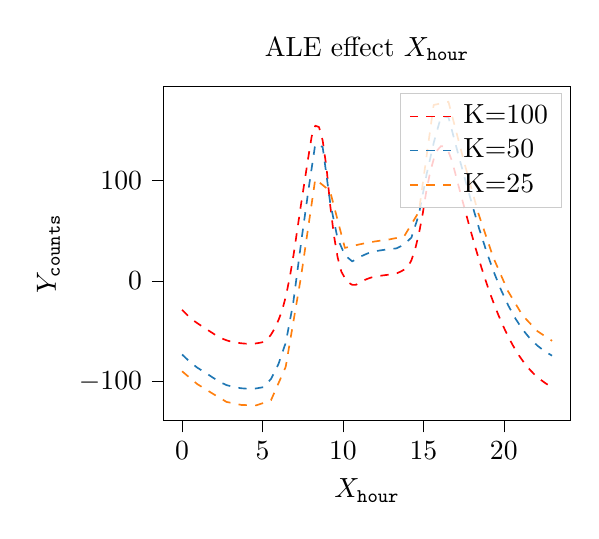
\begin{tikzpicture}

\definecolor{darkgray176}{RGB}{176,176,176}
\definecolor{darkorange25512714}{RGB}{255,127,14}
\definecolor{lightgray204}{RGB}{204,204,204}
\definecolor{steelblue31119180}{RGB}{31,119,180}

\begin{axis}[
legend cell align={left},
legend style={fill opacity=0.8, draw opacity=1, text opacity=1, draw=lightgray204},
tick align=outside,
tick pos=left,
title={ALE effect \(\displaystyle X_{\mathtt{hour}}\)},
x grid style={darkgray176},
xlabel={\(\displaystyle X_{\mathtt{hour}}\)},
xmin=-1.15, xmax=24.15,
xtick style={color=black},
y grid style={darkgray176},
ylabel={\(\displaystyle Y_{\mathtt{counts}}\)},
ymin=-138.606757724745, ymax=192.972018488682,
ytick style={color=black}
]
\addplot [semithick, red, dashed]
table {%
0 -28.6461296081543
0.299299240112305 -33.4844398498535
0.506506443023682 -36.5122833251953
0.73673677444458 -39.5242080688477
0.966966986656189 -42.1757049560547
1.74974977970123 -50.2825317382812
2.11811804771423 -54.0799827575684
2.32532525062561 -55.9247512817383
2.55555558204651 -57.6483955383301
2.78578567504883 -59.0419044494629
2.99299287796021 -60.0281982421875
3.24624633789062 -60.8593711853027
3.47647643089294 -61.46630859375
3.68368363380432 -61.8931121826172
3.91391396522522 -62.2204475402832
4.14414405822754 -62.3986968994141
4.37437438964844 -62.3219032287598
4.60460472106934 -61.990062713623
4.83483505249023 -61.4031791687012
5.04204225540161 -60.6504898071289
5.06506490707397 -60.5277214050293
5.29529523849487 -57.8714256286621
5.52552556991577 -53.4342956542969
5.75575590133667 -47.2163352966309
6.00900888442993 -38.2443809509277
6.21621608734131 -29.381742477417
6.44644641876221 -15.6827802658081
6.69969987869263 4.01029825210571
6.92992973327637 25.8215217590332
7.39039039611816 75.5200271606445
7.85085105895996 123.192329406738
8.05805778503418 143.596130371094
8.26526546478271 153.462203979492
8.28828811645508 154.119873046875
8.49549579620361 153.021850585938
8.51851844787598 152.449096679688
8.72572612762451 140.386978149414
8.74874877929688 138.58381652832
8.97897911071777 112.524017333984
9.20920944213867 75.0672760009766
9.43943977355957 45.3751182556152
9.66967010498047 23.4475517272949
9.89989948272705 9.28457546234131
10.1301298141479 2.64411807060242
10.3603601455688 -1.73881900310516
10.5675678253174 -3.74506211280823
10.5905904769897 -3.86423587799072
10.7977981567383 -3.84074091911316
10.8208208084106 -3.73213291168213
11.0740737915039 -1.27214574813843
11.3043041229248 0.624772906303406
11.5115118026733 2.059002161026
11.7417421340942 3.31951761245728
11.9719715118408 4.24510145187378
12.2482481002808 4.96000051498413
12.4784784317017 5.49322175979614
12.7087087631226 5.96644258499146
12.9159154891968 6.34280109405518
13.1001005172729 6.63770151138306
13.1231231689453 6.70726346969604
13.3303298950195 7.55532884597778
13.3763761520386 7.83442735671997
13.5835838317871 9.23264122009277
13.813814163208 11.3566951751709
14.0210208892822 13.7536668777466
14.0440444946289 14.2715625762939
14.2512512207031 20.38014793396
14.2972974777222 22.4057006835938
14.5045042037964 32.4857139587402
14.7347345352173 47.7849960327148
14.9649648666382 67.2124176025391
15.1951951980591 90.178352355957
15.42542552948 108.329772949219
15.6556558609009 121.666687011719
15.8628625869751 129.635528564453
15.9089088439941 130.593536376953
16.0930938720703 133.829193115234
16.1161155700684 133.91423034668
16.3233242034912 133.447540283203
16.3463459014893 133.071701049805
16.5535526275635 128.498184204102
16.5995998382568 126.696998596191
16.7837829589844 118.981163024902
16.8758754730225 113.421195983887
17.3363361358643 85.3754196166992
17.7967967987061 58.1768074035645
18.2112121582031 34.4831466674805
18.5335330963135 17.2674236297607
18.7407398223877 6.80826711654663
18.9709701538086 -4.24147033691406
19.2012004852295 -14.6806631088257
19.4084091186523 -23.5517692565918
19.6386394500732 -32.8170890808105
19.8688697814941 -41.4646186828613
20.0990982055664 -49.5049858093262
20.3063068389893 -56.2461433410645
20.5365371704102 -63.1648941040039
20.7667675018311 -69.4933547973633
20.9739742279053 -74.6995239257812
21.2272281646729 -80.4064331054688
21.4344348907471 -84.651123046875
21.664665222168 -88.8804550170898
21.8948955535889 -92.6121520996094
22.1481475830078 -96.1844940185547
22.3553562164307 -98.8407440185547
22.5855846405029 -101.486793518066
22.8158149719238 -103.820686340332
23 -105.487968444824
};
\addlegendentry{K=100}
\addplot [semithick, steelblue31119180, dashed]
table {%
0 -73.0295944213867
0.483483552932739 -80.3262100219727
0.943943977355957 -86.0722503662109
1.63463461399078 -93.052131652832
2.09509515762329 -97.846435546875
2.30230236053467 -100.020500183105
2.76276278495789 -103.408599853516
3.2232232093811 -105.34984588623
3.68368363380432 -106.578010559082
4.14414405822754 -107.09147644043
4.58158159255981 -106.740219116211
4.60460472106934 -106.712821960449
5.04204225540161 -105.514892578125
5.06506490707397 -105.378623962402
5.52552556991577 -97.3811645507812
5.98598575592041 -82.7204437255859
6.44644641876221 -61.2416725158691
6.906907081604 -22.0324935913086
7.45945930480957 45.1609420776367
7.89689683914185 94.8783798217773
8.26526546478271 134.32194519043
8.28828811645508 135.848922729492
8.72572612762451 133.169448852539
8.74874877929688 132.038055419922
9.20920944213867 77.4742279052734
9.66967010498047 42.0099868774414
10.1301298141479 25.4587116241455
10.5675678253174 19.581392288208
10.5905904769897 19.5158081054688
11.0510511398315 23.9011459350586
11.5115118026733 27.2109489440918
11.9719715118408 29.4452209472656
12.4554557800293 30.6770896911621
12.9159154891968 31.6511211395264
13.3303298950195 32.3632392883301
13.3533535003662 32.4914512634277
13.7907905578613 36.1472320556641
13.8368368148804 36.7766075134277
14.2512512207031 42.9912338256836
14.2742738723755 43.8286285400391
14.7117118835449 65.4701309204102
14.757758140564 69.0499725341797
15.2182178497314 107.198127746582
15.6556558609009 137.901489257812
16.0930938720703 163.001113891602
16.1161155700684 163.369003295898
16.5535526275635 162.597808837891
16.5765762329102 161.576858520508
17.2442436218262 121.308631896973
17.6816825866699 95.7949066162109
18.1421413421631 69.7332916259766
18.4644641876221 52.1377601623535
18.9249248504639 29.2084808349609
19.362361907959 9.56418228149414
19.8228225708008 -8.68426704406738
20.2832832336426 -24.4933090209961
20.7207202911377 -37.3236122131348
21.1811809539795 -48.4314765930176
21.6416416168213 -57.4496726989746
22.1021022796631 -64.4142456054688
22.5625629425049 -70.0410766601562
23 -74.1791915893555
};
\addlegendentry{K=50}
\addplot [semithick, darkorange25512714, dashed]
table {%
0 -89.7076110839844
0.943943977355957 -102.404815673828
1.97997999191284 -112.664199829102
2.76276278495789 -120.120399475098
3.68368363380432 -123.145240783691
4.58158159255981 -123.534996032715
4.60460472106934 -123.51879119873
5.50250244140625 -118.79963684082
5.52552556991577 -118.507827758789
6.42342329025269 -86.0327835083008
6.44644641876221 -84.83203125
7.39039039611816 3.69972920417786
8.26526546478271 99.6076049804688
8.28828811645508 101.115272521973
9.18618583679199 89.4567947387695
9.20920944213867 88.7125854492188
10.1071071624756 33.6399116516113
10.1301298141479 32.8881683349609
11.0510511398315 36.4285697937012
11.9719715118408 39.2134017944336
12.8928928375244 41.2662658691406
13.7907905578613 44.1628112792969
13.813814163208 44.5594520568848
14.7117118835449 68.4099655151367
14.7347345352173 70.3300552368164
15.6326322555542 173.919738769531
15.6556558609009 174.823348999023
16.5535526275635 177.900253295898
16.5765762329102 176.900024414062
17.5665664672852 116.187698364258
18.4184188842773 67.2121658325195
19.3393402099609 23.6039810180664
20.2602596282959 -10.096302986145
21.1581573486328 -34.0074882507324
21.3193187713623 -36.7692565917969
22.0790786743164 -49.7056350708008
22.3783779144287 -52.8796615600586
23 -59.459545135498
};
\addlegendentry{K=25}
\end{axis}

\end{tikzpicture}
}
    \caption{Bike-Sharing Dataset. Feature effect plots on \(X_{\texttt{hour}}\): (Left)
      DALE vs ALE for \(K=200\). (Center) DALE plots for
      \(K = \{25, 50, 100\}\). (Right) ALE plots for
      \(K = \{25, 50, 100\}\)}
  \label{fig:bike-sharing-feature-3}
\end{figure}


\begin{table}
  \caption{Evaluation of DALE and ALE approximation when lowering the
    number of bins \(K\). The ground-truth effect has been computed
    for \(K=200\).}
  \label{tab:bike-sharing-accuracy}
  \centering
  \begin{tabular}{c|c|c|c|c|c}
    \multicolumn{6}{c}{Accuracy on Bike-Sharing Dataset - Feature \(X_{\mathtt{hour}}\)} \\
    \hline \hline
    & & \multicolumn{4}{|c}{Number of bins} \\
    \hline
    & & 100 & 50 & 25 & 15 \\
    \hline
    \hline
    \multirow{2}{*}{\(\mathtt{NMSE}\)} & \(\dale\) & \textbf{0.007} & \textbf{0.01} & \textbf{0.03} & \textbf{0.09} \\
    & \(\alep\) & 0.04 & 0.43 & 0.79 & 0.83 \\
    \hline
  \end{tabular}
\end{table}


\section{Conclusion and Future Work}
This paper introduced DALE, an efficient and robust-to-OOD
approximation for ALE, the state-of-the-art method for feature effect
analysis. First, we explored the advantages of ALE over the other two
renowned feature effect methods, PDP and MPlots. However, ALE's
approximation scales poorly in big and high-dimensional datasets and
suffers from OOD sampling in cases with limited samples. For
addressing these deficiencies, we proposed DALE, a fast and
on-distribution alternative. We presented the method and discussed the
advantages over the typical ALE approximation. We proved that under
some hypotheses, our proposal is an unbiased estimator of ALE and we
presented a method for quantifying the uncertainty of the explanation,
i.e. the standard error of the approximation. The experiments verify
the aforementioned claims. DALE significantly improves the efficiency
of ALE's approximation by orders of magnitude and secures that local
effect estimations come from on-distribution samples. The latter leads
to more accurate feature effect plots when the bins are wide and the
black-box function changes away from the data generating distribution.

The computational efficiency of DALE delivers a substantial margin for
future extensions. A significant advantage of our proposal is that
effects are computed once on the training set points and can be reused
in different-size bins. The decision for the bin density, i.e., the
resolution of the plot, can be taken afterwards. Therefore, DALE
permits creating feature effect plots at different resolutions with
near-zero computational overhead, which can be embedded into a
multi-resolution feature effect plots framework.


\acks{We thank Eirini Ntoutsi for her insightful comments in the
  draft versions of the paper and Giorgos Giannopoulos for the valuable
  discussions while forming the initial idea.

  \noindent
  This research was funded by the EU (H2020-EU.2.1.1.) project,
  “XMANAI: Explainable Manufacturing Artificial Intelligence" -
  ICT-38-2020 - Artificial intelligence for manufacturing, Grant
  agreement ID: 957362.
}



%\bibliographystyle{plain}
\bibliography{gkolemis22-bib}

% \appendix

% \section{First Appendix}\label{apd:first}

% This is the first appendix.

% \section{Second Appendix}\label{apd:second}

% This is the second appendix.


\end{document}
